%%%%%%%%%%%%%%%%%%%%%%%%%%%%%%%%%%%%%%%%%%%%%%%%%%%%%%%%%%%%%%%
%% OXFORD THESIS TEMPLATE

% Use this template to produce a standard thesis that meets the Oxford University requirements for DPhil submission
%
% Originally by Keith A. Gillow (gillow@maths.ox.ac.uk), 1997
% Modified by Sam Evans (sam@samuelevansresearch.org), 2007
% Modified by John McManigle (john@oxfordechoes.com), 2015
%
% This version Copyright (c) 2015-2023 John McManigle
%
% Broad permissions are granted to use, modify, and distribute this software
% as specified in the MIT License included in this distribution's LICENSE file.
%

% I've (John) tried to comment this file extensively, so read through it to see how to use the various options.  Remember
% that in LaTeX, any line starting with a % is NOT executed.  Several places below, you have a choice of which line to use
% out of multiple options (eg draft vs final, for PDF vs for binding, etc.)  When you pick one, add a % to the beginning of
% the lines you don't want.


%%%%% CHOOSE PAGE LAYOUT
% The most common choices should be below.  You can also do other things, like replacing "a4paper" with "letterpaper", etc.

% This one will format for two-sided binding (ie left and right pages have mirror margins; blank pages inserted where needed):
\documentclass[a4paper]{ociamthesis_modified}
% This one will format for one-sided binding (ie left margin > right margin; no extra blank pages):
%\documentclass[a4paper]{ociamthesis}
% This one will format for PDF output (ie equal margins, no extra blank pages):
%\documentclass[a4paper,nobind]{ociamthesis} 



%%%%% SELECT YOUR DRAFT OPTIONS
% Three options going on here; use in any combination.  But remember to turn the first two off before
% generating a PDF to send to the printer!

% This adds a "DRAFT" footer to every normal page.  (The first page of each chapter is not a "normal" page.)
% \fancyfoot[C]{\emph{DRAFT Printed on \today}}  

% This highlights (in blue) corrections marked with (for words) \mccorrect{blah} or (for whole
% paragraphs) \begin{mccorrection} . . . \end{mccorrection}.  This can be useful for sending a PDF of
% your corrected thesis to your examiners for review.  Turn it off, and the blue disappears.
\correctionstrue


%%%%% BIBLIOGRAPHY SETUP
% Note that your bibliography will require some tweaking depending on your department, preferred format, etc.
% The options included below are just very basic "sciencey" and "humanitiesey" options to get started.
% If you've not used LaTeX before, I recommend reading a little about biblatex/biber and getting started with it.
% If you're already a LaTeX pro and are used to natbib or something, modify as necessary.
% Either way, you'll have to choose and configure an appropriate bibliography format...

% The science-type option: numerical in-text citation with references in order of appearance.
% \usepackage[style=numeric-comp, sorting=none, backend=biber, doi=false, isbn=false]{biblatex}
% \newcommand*{\bibtitle}{References}
\bibliographystyle{plainnat}
\usepackage{pdfpages}
% \usepackage{amsmath}
% \usepackage{amsthm}
% \usepackage{amsfonts}
% \usepackage{thmtools,thm-restate}
% \usepackage{bbm}
% \usepackage{mathtools}
\usepackage{natbib}

\usepackage{subcaption}
\usepackage[ruled,vlined]{algorithm2e}
\usepackage{caption}
\usepackage{graphicx}
% \usepackage{subfigure}
\usepackage{amsmath}
\usepackage{amsthm}
\usepackage{amsfonts}
\usepackage{thmtools,thm-restate}
\usepackage{bbm}
\usepackage{mathtools}
\usepackage{authblk}

% \usepackage[hidelinks]{hyperref}
% \usepackage[square,sort,comma,numbers]{natbib}
% \newtheorem{lemma}{Lemma}
% \newtheorem{theorem}{Theorem}
% \newtheorem{definition}{Definition}
% \newtheorem{sublemma}{Lemma}[lemma]
% \newtheorem{corollary}{Corollary}
\newcommand{\indep}{\perp \!\!\! \perp}
% \usepackage[backend=biber]{biblatex}
% \addbibresource{references.bib}
% \PassOptionsToPackage{numbers}{natbib}
% \setcitestyle{numerical, square}
% \setcitestyle{authoryear,open={(},close={)}}
\usepackage{capt-of}
% \usepackage{enumerate}
% \hypersetup{colorlinks,citecolor=blue}
\usepackage{comment}
% \newcommand{\faaiz}[1]{\textcolor{red}{{\bf Faaiz:} #1}}
\newcommand{\faaiz}[1]{#1}
% \newcommand{\R}[1]{\textcolor{red}{#1}}
\newcommand{\R}{\mathbb{R}}

\newcommand{\jef}[1]{\textcolor{blue}{{\bf Jef:} #1}}
\usepackage{amsmath}
\DeclareMathOperator*{\argmax}{arg\,max}
\DeclareMathOperator*{\argmin}{arg\,min}
\usepackage{comment}
\usepackage{microtype}
\usepackage{booktabs}
\usepackage{centernot}


%%%%%%%%%%%%%%% colors

\usepackage[many]{tcolorbox}
\usepackage{xcolor}
\usepackage{color}
\usepackage{colortbl}

%
\definecolor{MyLightGray}{gray}{0.925}
\definecolor{MyDarkGray}{gray}{0.55}
\definecolor{myblue}{rgb}{0.00, 0.45, 0.70}
\definecolor{mygreen}{rgb}{0.01, 0.62, 0.45}
\definecolor{myred}{rgb}{0.84, 0.37, 0.00}

%
%
\PassOptionsToPackage{hyphens}{url}
% \usepackage[hidelinks]{hyperref}
\usepackage{hyperref}
%
%
%
%
%
%

%
\definecolor{blue}{RGB}{0,114,178}
\definecolor{red}{RGB}{213,80,20}
%
\definecolor{green}{RGB}{0,158,115}
\definecolor{purple}{RGB}{204,121,167}
\definecolor{orange}{RGB}{230,159, 0}
\definecolor{pink}{RGB}{204,121,167}

\definecolor{ourmethod}{gray}{0.93}


%
\definecolor{sns0}{HTML}{1f77b4}
\definecolor{sns1}{HTML}{ff7f0e}
\definecolor{sns2}{HTML}{2ca02c}
\definecolor{sns3}{HTML}{d62728}
\definecolor{sns4}{HTML}{9467bd}
\definecolor{sns5}{HTML}{8c564b}

%
%
%
%
%
%
%
%
%


%
\definecolor{sns-orange}{HTML}{ff7f0e}
\definecolor{sns-ambiguous}{HTML}{00528C}
\definecolor{sns-nonambiguous}{HTML}{2CA9FF}
\definecolor{sns-blue}{HTML}{1f77b4}
%

%

%
\definecolor{solarized@base03}{HTML}{002B36}
\definecolor{solarized@base02}{HTML}{073642}
\definecolor{solarized@base01}{HTML}{586e75}
\definecolor{solarized@base00}{HTML}{657b83}
\definecolor{solarized@base0}{HTML}{839496}
\definecolor{solarized@base1}{HTML}{93a1a1}
\definecolor{solarized@base2}{HTML}{EEE8D5}
\definecolor{solarized@base3}{HTML}{FDF6E3}
\definecolor{solarized@yellow}{HTML}{B58900}
\definecolor{solarized@orange}{HTML}{CB4B16}
\definecolor{solarized@red}{HTML}{DC322F}
\definecolor{solarized@magenta}{HTML}{D33682}
\definecolor{solarized@violet}{HTML}{6C71C4}
\definecolor{solarized@blue}{HTML}{268BD2}
\definecolor{solarized@cyan}{HTML}{2AA198}
\definecolor{solarized@green}{HTML}{859900}



\theoremstyle{plain}

% Redefine the theorem environment to be enclosed in mainresult
\newtcolorbox{mainresult}{colback=solarized@violet!5!white,
colframe=solarized@violet,parbox, left=0.5mm, right=0.5mm,top=0.5mm,bottom=0.5mm}

% \newtcolorbox{mainresult}[1][]{colback=solarized@violet!5!white,
% colframe=solarized@violet, parbox=true, left=0.5mm, right=0.5mm, 
% top=0.5mm, bottom=0.5mm, breakable, title={#1}}

% Define the mainresult environment
\newtcolorbox{mainresultwithtitle}[2][]{colback=solarized@violet!7!white,
colframe=solarized@violet!7, 
colbacktitle=solarized@violet,
parbox=false, 
left=0.5mm, 
right=0.5mm, 
top=0.5mm, 
bottom=0.5mm, 
% breakable, 
title={#2}, 
#1}

% \newtcolorbox{importantresult}{breakable,colback=solarized@yellow!5!white,
% colframe=solarized@yellow,parbox, left=0.5mm, right=0.5mm,top=0.5mm,bottom=0.5mm}

% \newtcolorbox{importantresult}{
%   breakable,
%   colback=solarized@yellow!5!white,
%   colframe=solarized@yellow,
%   parbox=false,
%   left=0.5mm,
%   right=0.5mm,
%   top=0.5mm,
%   bottom=0.5mm,
%   % before upper={\setlength{\parskip}{1em}},
%   before={\setlength{\parskip}{1em}},
%   before upper={\vspace{-2.1em}}, % Remove the vertical space before the content
% % before upper={\vspace{-\baselineskip}}, % Remove the vertical space before the content
% }
\newtcolorbox{importantresultwithtitle}[2][]{
  % breakable,
  colback=solarized@cyan!7!white,
  colframe=solarized@cyan!7,
  colbacktitle=solarized@cyan,
  parbox=false,
  left=0.5mm,
  right=0.5mm,
  top=0.5mm,
  bottom=0.5mm,
  title={#2}, 
  #1
}


\newtcolorbox{whiteresult}{colback=solarized@violet!2!white,
colframe=solarized@violet,parbox, left=0.5mm, right=0.5mm,top=0.5mm,bottom=0.5mm}


\newtheorem{theorem}{Theorem}[section]
% Save the original theorem environment
\let\oldtheorem\theorem

% \renewenvironment{theorem}[1][\unskip]
%   {\begin{mainresult}\ifthenelse{\equal{#1}{\unskip}}{\oldtheorem}{\oldtheorem[#1]}}
%   {\end{mainresult}}


% \newcounter{theorem}[section]
% \renewcommand{\thetheorem}{\thesection.\arabic{theorem}}

% Define a new environment for assumptions within mainresult
\renewenvironment{theorem}[1][]
 {\refstepcounter{theorem}
  \begin{mainresultwithtitle}[title={Theorem \thetheorem\ifx#1\empty\else~(#1)\fi}]\noindent}
 {\end{mainresultwithtitle}}


% \renewenvironment{theorem}[1][\unskip]{%
%   \begin{mainresult}
%   \ifx#1\unskip\oldtheorem\else\oldtheorem[#1]\fi%
% }{%
%   % \endoldtheorem
%   \end{mainresult}
% }

\newcounter{proposition}[section]
\renewcommand{\theproposition}{\thesection.\arabic{proposition}}

% Define a new environment for assumptions within mainresult
\newenvironment{proposition}[1][]
 {\refstepcounter{proposition}
  \begin{mainresultwithtitle}[title={Proposition \theproposition\ifx#1\empty\else~(#1)\fi}]\noindent}
 {\end{mainresultwithtitle}}

% \newtheorem{proposition}[theorem]{Proposition}
% \let\oldproposition\proposition
% \renewenvironment{proposition}[1][\unskip]{%
%   \begin{mainresult}
%   \ifx#1\unskip\oldproposition\else\oldproposition[#1]\fi%
% }{%
%   % \endoldtheorem
%   \end{mainresult}
% }


\newcounter{lemma}[section]
\renewcommand{\thelemma}{\thesection.\arabic{lemma}}

% Define a new environment for assumptions within mainresult
\newenvironment{lemma}[1][]
 {\refstepcounter{lemma}
  \begin{mainresultwithtitle}[title={Lemma \thelemma\ifx#1\empty\else~(#1)\fi}]\noindent}
 {\end{mainresultwithtitle}}

% \newtheorem{lemma}[theorem]{Lemma}
% \let\oldlemma\lemma
% \renewenvironment{lemma}[1][\unskip]{%
%   \begin{mainresult}
%   \ifx#1\unskip\oldlemma\else\oldlemma[#1]\fi%
% }{%
%   \end{mainresult}
% }


\newcounter{corollary}[section]
\renewcommand{\thecorollary}{\thesection.\arabic{corollary}}

% Define a new environment for assumptions within mainresult
\newenvironment{corollary}[1][]
 {\refstepcounter{corollary}
  \begin{mainresultwithtitle}[title={Corollary \thecorollary\ifx#1\empty\else~(#1)\fi}]\noindent}
 {\end{mainresultwithtitle}}

 
% \newtheorem{corollary}[theorem]{Corollary}
% \let\oldcorollary\corollary
% \renewenvironment{corollary}[1][\unskip]{%
%   \begin{mainresult}
%   \ifx#1\unskip\oldcorollary\else\oldcorollary[#1]\fi%
% }{%
%   \end{mainresult}
% }

\newcounter{definition}[section]
\renewcommand{\thedefinition}{\thesection.\arabic{definition}}

% Define a new environment for assumptions within mainresult
\newenvironment{definition}[1][]
 {\refstepcounter{definition}
  \begin{importantresultwithtitle}[title={Definition \thedefinition\ifx#1\empty\else~(#1)\fi}]\noindent}
 {\end{importantresultwithtitle}}

% \theoremstyle{definition}
% \newtheorem{definition}[theorem]{Definition}
% \let\olddefinition\definition
% \renewenvironment{definition}[1][\unskip]{%
%   \begin{importantresult}
%   \ifx#1\unskip\olddefinition\else\olddefinition[#1]\fi%
% }{%
%   \end{importantresult}
% }

\newtheorem{assumption}[theorem]{Assumption}
% \let\oldassumption\assumption
% \renewenvironment{assumption}[1][\unskip]{%
%   \begin{mainresult}%
%   \ifx#1\unskip\oldassumption\else\oldassumption[#1]\fi%
% }{%
%   \end{mainresult}%
% }

% \newcounter{assumption}[section]
% \renewcommand{\theassumption}{\thesection.\arabic{assumption}}

% Define a new environment for assumptions within mainresult
% \newenvironment{assumption}[1][]
%  {\refstepcounter{assumption}
%   \begin{mainresultwithtitle}[title={Assumption \theassumption\ifx#1\empty\else~(#1)\fi}]\noindent}
%  {\end{mainresultwithtitle}}


 \newcounter{limitation}[section]
\renewcommand{\thelimitation}{\thesection.\arabic{limitation}}

% Define a new environment for assumptions within mainresult
\newenvironment{limitation}[1][]
 {\refstepcounter{limitation}
  \begin{mainresultwithtitle}[title={Limitation \thelimitation\ifx#1\empty\else~(#1)\fi}]\noindent}
 {\end{mainresultwithtitle}}

% \newtheorem{proposition}{Proposition}
% \theoremstyle{definition}
\newcounter{remark}[section]
\renewcommand{\theremark}{\thesection.\arabic{remark}}

% Define a new environment for assumptions within mainresult
\newenvironment{remark}[1][]
 {\refstepcounter{remark}
  \begin{importantresultwithtitle}[title={Remark \theremark\ifx#1\empty\else~(#1)\fi}]\noindent}
 {\end{importantresultwithtitle}}


% \newtheorem{remark}[theorem]{Remark}
% \let\oldremark\remark
% \renewenvironment{remark}[1][\unskip]{%
%   \begin{importantresult}
%   \ifx#1\unskip\oldremark\else\oldremark[#1]\fi%
% }{%
%   \end{importantresult}
% }

\newcommand{\red}[1]{\textcolor{red}{#1}}
\newcommand{\p}[0]{\mathbb{P}}
\newcommand{\E}[0]{\mathbb{E}}
\newcommand{\tarprob}[0]{\mathbb{P}_{(X,Y)\sim P^{\pi^*}_{X,Y}}}
\newcommand{\ttar}[0]{\mathbb{P}_{(X,Y)\sim \tilde{P}^{\pi^*}_{X,Y}}}
\newcommand{\behprob}[0]{\mathbb{P}_{(X,Y)\sim P^{\pi^b}_{X,Y}}}
\newcommand{\expb}[0]{\mathbb{E}_{(X,Y)\sim P^{\pi^b}_{X,Y}}}
\newcommand{\expt}[0]{\mathbb{E}_{(X,Y)\sim P^{\pi^*}_{X,Y}}}
\newcommand{\exptt}[0]{\mathbb{E}_{(\tilde{X},\tilde{Y})\sim P^{\pi^*}_{X,Y}}}
\newcommand{\expat}[0]{\mathbb{E}_{(X,Y)\sim \tilde{P}^{\pi^*}_{X,Y}}}
\newcommand{\expatt}[0]{\mathbb{E}_{(\tilde{X},\tilde{Y})\sim \tilde{P}^{\pi^*}_{X,Y}}}

\newcommand{\behcal}[0]{\mathbb{P}_{(X_i,Y_i)\sim P^{\pi^b}_{X,Y}}}
\newcommand{\expbcal}[0]{\mathbb{E}_{(X_i, Y_i) \sim P^{\pi^b}_{X,Y}}}


\newcommand{\todo}[1]{\textcolor{red}{#1}}
\newcommand{\ind}{\mathbbm{1}}
\newcommand{\Aspace}{\mathcal{A}}
\newcommand{\Xspace}{\mathcal{X}}



%%%%%%%%%%%%%% DT %%%%%%%%%%%%%%%%%



\newcommand{\ceil}[1]{\left\lceil#1\right\rceil}
\newcommand{\floor}[1]{\left\lfloor#1\right\rfloor}
\newcommand{\set}[1]{\left\{#1\right\}}
\newcommand{\abs}[1]{|#1|}
\newcommand{\norm}[1]{\left\lVert#1\right\rVert}
\DeclareMathOperator*{\supp}{supp}

\newcommand{\Var}{\mathrm{Var}}
\newcommand{\Prob}{\mathbb{P}}
\newcommand{\iid}{\overset{\mathrm{iid}}{\sim}}
\newcommand{\eqas}{\overset{\mathrm{a.s.}}{=}}
\newcommand{\Law}{\mathrm{Law}}
\newcommand{\io}{\mathrm{i.o.}}
\newcommand{\ev}{\mathrm{ev.}}
\newcommand{\eqd}{\overset{\mathrm{d}}{=}}
\newcommand{\neqd}{\overset{\mathrm{d}}{\neq}}

\newcommand{\Cauchy}{\mathrm{Cauchy}}
\newcommand{\Normal}{\mathrm{Normal}}
\newcommand{\Bernoulli}{\mathrm{Bernoulli}}
\newcommand{\Uniform}{\mathrm{Uniform}}
\newcommand{\Dirac}{\mathrm{Dirac}}

\DeclarePairedDelimiterX{\infdivx}[2]{(}{)}{#1\;\delimsize\|\;#2}
\newcommand{\KL}{D_{\mathrm{KL}}\infdivx*}
\newcommand{\JS}{\mathrm{JS}\infdivx*}
\newcommand{\fdiv}{\mathrm{D}_f\infdivx*}

\newcommand\ci{\perp\!\!\!\perp}

\DeclareMathOperator*{\ITE}{ITE}

\newcommand{\twinsupscript}{\mathsf{twin}}

\newcommand{\dee}{\mathrm{d}}

\newcommand{\Xspacedim}{d}
\newcommand{\A}{A}
\newcommand{\X}{X}
\newcommand{\xx}{x}
\newcommand{\Xt}{\widehat{\X}}
\newcommand{\At}{\A^\twinsupscript}
\newcommand{\ax}{a}

\newcommand{\Hspace}{\mathcal{H}}
\newcommand{\Hx}{H}
\newcommand{\hx}{h}

\newcommand{\Sx}{S}
\newcommand{\St}{\Sx^\twinsupscript}
\newcommand{\Sspace}{\mathcal{S}}
\newcommand{\Stspace}{\Sspace^\twinsupscript}
\newcommand{\sx}{s}

\newcommand{\Espace}{\mathcal{E}}
\newcommand{\Etspace}{\Espace^\twinsupscript}
\newcommand{\Eps}{\epsilon}
\newcommand{\Epst}{\Eps^\twinsupscript}
\newcommand{\ex}{e}
\newcommand{\agtsupscript}{\mathsf{agent}}
\newcommand{\Easpace}{\Espace^\agtsupscript}
\newcommand{\Epsa}{\Eps^\agtsupscript}
\newcommand{\epsa}{\ex^\agtsupscript}

\newcommand{\pix}{\pi}


\newcommand{\nx}{n}
\newcommand{\ix}{i}

\newcommand{\gx}{g}
\newcommand{\gxt}{\gx^\twinsupscript}
% \newcommand{\hx}{h}
\newcommand{\hxt}{\hx^\twinsupscript}

% \newcommand{\N}{T}
\newcommand{\tx}{t}
\newcommand{\B}{B}
\newcommand{\N}{N}
\newcommand{\T}{T}

\newcommand{\fx}{f}

\newcommand{\lo}[1]{#1_{\mathrm{lo}}}
\newcommand{\up}[1]{#1_{\mathrm{up}}}
\newcommand{\loup}[1]{{#1_{\mathrm{lo} \cap \mathrm{up}}}}

\newcommand{\Y}{Y}
\newcommand{\Yt}{\widehat{Y}}
\newcommand{\ylo}{\lo{y}}
\newcommand{\yup}{\up{y}}
\newcommand{\ytlo}{\lo{y^\twinsupscript}}
\newcommand{\ytup}{\up{y^\twinsupscript}}
\newcommand{\Ylo}{\lo{\Y}}
\newcommand{\Yup}{\up{\Y}}

\newcommand{\Q}{Q}
\newcommand{\Qt}{\widehat{\Q}}
\newcommand{\Qlo}{\lo{\Q}}
\newcommand{\Qup}{\up{\Q}}

\newcommand{\Qlohat}{\lo{\widehat{\Q}}}
\newcommand{\Quphat}{\up{\widehat{\Q}}}

\newcommand{\qlo}[1]{\lo{R}^{#1}}
\newcommand{\qup}[1]{\up{R}^{#1}}
\newcommand{\qt}[1]{\widehat{R}^{#1}}

\newcommand{\mybar}[1]{\makebox[0pt]{$\phantom{#1}\overline{\phantom{#1}}$}#1}
\newcommand{\Ylobar}{\lo{\mybar{\Y}}}
\newcommand{\Yupbar}{\up{\mybar{\Y}}}

\newcommand{\YClmean}{{\lo{\mu}}}
\newcommand{\YCumean}{{\up{\mu}}}
\newcommand{\Ytmean}{\widehat{\mu}}
\newcommand{\CIlen}{\Delta}
\newcommand{\CIlolen}{\lo{\Delta}}
\newcommand{\CIuplen}{\up{\Delta}}

\newcommand{\Hyp}{\mathcal{H}}
\newcommand{\Hlo}{\lo{\Hyp}}
\newcommand{\plo}{p_{\textup{lo}}}
\newcommand{\Hup}{\up{\Hyp}}
\newcommand{\pup}{p_{\textup{up}}}
\newcommand{\Hloup}{\loup{\Hyp}}
\newcommand{\test}{\delta}
\newcommand{\testlo}{\lo{\test}}
\newcommand{\testup}{\up{\test}}
\newcommand{\testloup}{\loup{\test}}
\newcommand{\reject}{\mathsf{reject}}
\newcommand{\accept}{\mathsf{retain}}

\newcommand{\D}{\mathcal{D}}
\newcommand{\Dt}{\widehat{\D}}

\newcommand{\QR}{R}
\newcommand{\QtR}{\widehat{R}}

\newcommand{\nsplitx}{n_{\mathrm{split}}}

\newcommand{\twinfunction}{h}
\newcommand{\twinnoise}{U}
\newcommand{\ux}{u}

\newcommand{\rob}[1]{{\color{blue}$\langle$ \textsc{Rob:} {\it #1} $\rangle$}}
% \newcommand{\Rob}[1]{{\color{orange}$\langle$ \textsc{Rob:} {\it #1} $\rangle$}}
% \newcommand{\faaiz}[1]{}
% \newcommand{\todiscuss}[1]{{\color{green}$\langle$ \textsc{To discuss:} {\it #1} $\rangle$}}

\newcommand{\Z}{Z}
\newcommand{\Zt}{\widehat{Z}}

\newcommand{\clip}{\mathrm{clip}}

% \newcommand{\Rob}[1]{}
% \newcommand{\rob}[1]{}
% \newcommand{\todiscuss}[1]{}
% \newcommand{\faaiz}[1]{}

\newcommand{\Pobs}{{P_\mathrm{obs}}}
\newcommand{\Pobstilde}{{\tilde{P}_\mathrm{obs}}}


\newcommand{\AppendixName}{Appendix\xspace}
\usepackage{tabularx}

% \newtheorem{manualtheoreminner}{Theorem}

% \newenvironment{manualtheorem}[1]{%
%   \renewcommand\themanualtheoreminner{#1}%
%   \manualtheoreminner
% }{\endmanualtheoreminner}


% \newenvironment{manualtheorem}[1]{%
%   \begin{mainresult}    
%   \renewcommand\themanualtheoreminner{#1}%
%   \manualtheoreminner
% }{
%     \endmanualtheoreminner 
%     \end{mainresult}
% }

% \newenvironment{manualtheorem}[1]{%
%   \renewcommand\themanualtheoreminner{#1}%
%   \manualtheoreminner
% }{
%     \endmanualtheoreminner 
%     \end{mainresult}
% }
\newenvironment{manualtheorem}[1]
 {\begin{mainresultwithtitle}[title={Theorem #1}]\noindent}
 {\end{mainresultwithtitle}}

% \newtheorem{manualpropositioninner}{Proposition}
% \newenvironment{manualproposition}[1]{%
%   \renewcommand\themanualpropositioninner{#1}%
%   \manualpropositioninner
% }{\endmanualpropositioninner}


% \newtheorem{manualpropositioninner}{Proposition}
% \newenvironment{manualproposition}[1]{%
% \begin{mainresult}
%   \renewcommand\themanualpropositioninner{#1}%
%   \manualpropositioninner
% }{
%     \endmanualpropositioninner
%     \end{mainresult}
% }
\newenvironment{manualproposition}[1]
 {\begin{mainresultwithtitle}[title={Proposition #1}]\noindent}
 {\end{mainresultwithtitle}}


%%%%%%%%%%%%%%%%%%%%%%%%% MR %%%%%%%%%%%%%%%%%%%%

\newcommand{\tar}[0]{\pi^*}
\newcommand{\beh}[0]{\pi^b}
\newcommand{\hatbeh}[0]{\widehat{\pi}^b}
\newcommand{\ptar}[0]{p_{\pi^*}}
\newcommand{\Etar}[0]{\mathbb{E}_{\pi^*}}
\newcommand{\Etarred}[0]{\mathbb{E}_{\textcolor{red}{\pi^*}}}
\newcommand{\Ebeh}[0]{\mathbb{E}_{\pi^b}}
\newcommand{\Ebehblue}[0]{\mathbb{E}_{\textcolor{blue}{\pi^b}}}
\newcommand{\Vtar}[0]{\textup{Var}_{\pi^*}}
\newcommand{\Vbeh}[0]{\textup{Var}_{\pi^b}}
\newcommand{\V}[0]{\textup{Var}}

\newcommand{\pbeh}[0]{p_{\pi^b}}
\newcommand{\thetacdr}[0]{\hat{\theta}_{\textup{CDR}}}
\newcommand{\thetadr}[0]{\hat{\theta}_{\textup{DR}}}
\newcommand{\thetamr}[0]{\hat{\theta}_{\textup{MR}}}
\newcommand{\thetaipw}[0]{\hat{\theta}_{\textup{IPW}}}
\newcommand{\thetaswitch}[0]{\hat{\theta}_{\textup{SwitchDR}}}
\newcommand{\thetadros}[0]{\hat{\theta}_{\textup{DRos}}}
\newcommand{\approxipw}[0]{\tilde{\theta}_{\textup{IPW}}}
\newcommand{\approxmr}[0]{\tilde{\theta}_{\textup{MR}}}
\newcommand{\thetagmdr}[0]{\tilde{\theta}_{\textup{DM-DR}}}
\newcommand{\ipw}[0]{\textup{IPW}}
\newcommand{\cdr}[0]{\textup{CDR}}
\newcommand{\mr}[0]{\textup{MR}}
\newcommand{\dr}[0]{\textup{DR}}
\newcommand{\ate}[0]{\textup{ATE}}
\newcommand{\var}[0]{\textup{Var}}
\newcommand{\Yspace}[0]{\mathcal{Y}}

\newcommand{\iidsim}[0]{\overset{\textup{i.i.d.}}{\sim}}


\newcommand{\Dtr}[0]{\mathcal{D}_{\textup{tr}}}
\newcommand{\Dev}[0]{\mathcal{D}_{\textup{ev}}}
\newcommand{\gt}[0]{{\textup{gt}}}

\newcommand{\ateipw}{\widehat{\ate}_{\ipw}}
\newcommand{\atemr}{\widehat{\ate}_{\mr}}
\newcommand{\atedr}{\widehat{\ate}_{\dr}}
\newcommand{\thetasnmr}{\theta_{\textup{SNMR}}}
\newcommand{\tr}{{\textup{tr}}}
\newcommand{\myparagraph}[1]{\paragraph{#1}}
\newcommand{\flag}[1]{#1}
\usepackage{wrapfig}
\usepackage{tikz}
\usepackage{ifthen}
\usepackage{rotating}

% Define a boolean flag
\newboolean{compilePapers}
\newboolean{compileAppendices}
% Set the flag to true or false
\setboolean{compilePapers}{true}% or \setboolean{myflag}{false}

\setboolean{compileAppendices}{true}


\AtBeginEnvironment{subappendices}{%
\chapter*{Appendix}
\addcontentsline{toc}{chapter}{Appendices}
\counterwithin{figure}{section}
\counterwithin{table}{section}
}


% The humanities-type option: author-year in-text citation with an alphabetical works cited.
%\usepackage[style=authoryear, sorting=nyt, backend=biber, maxcitenames=2, useprefix, doi=false, isbn=false]{biblatex}
%\newcommand*{\bibtitle}{Works Cited}

% This makes the bibliography left-aligned (not 'justified') and slightly smaller font.
\renewcommand*{\bibfont}{\raggedright\small}

% Change this to the name of your .bib file (usually exported from a citation manager like Zotero or EndNote).
% \addbibresource{references.bib}


% Uncomment this if you want equation numbers per section (2.3.12), instead of per chapter (2.18):
%\numberwithin{equation}{subsection}



%%%%% THESIS / TITLE PAGE INFORMATION
% Everybody needs to complete the following:
\title{Uncertainty Quantification and Causal Considerations for Off-Policy Decision Making}
\author{Muhammad Faaiz Taufiq}
\college{Wolfson College}

% Master's candidates who require the alternate title page (with candidate number and word count)
% must also un-comment and complete the following three lines:
%\masterssubmissiontrue
%\candidateno{933516}
%\wordcount{28,815}

% Uncomment the following line if your degree also includes exams (eg most masters):
%\renewcommand{\submittedtext}{Submitted in partial completion of the}
% Your full degree name.  (But remember that DPhils aren't "in" anything.  They're just DPhils.)
\degree{Doctor of Philosophy}
% Term and year of submission, or date if your board requires (eg most masters)
\degreedate{Michaelmas 2024}


%%%%% YOUR OWN PERSONAL MACROS
% This is a good place to dump your own LaTeX macros as they come up.

% To make text superscripts shortcuts
	\renewcommand{\th}{\textsuperscript{th}} % ex: I won 4\th place
	\newcommand{\nd}{\textsuperscript{nd}}
	\renewcommand{\st}{\textsuperscript{st}}
	\newcommand{\rd}{\textsuperscript{rd}}

%%%%% THE ACTUAL DOCUMENT STARTS HERE
\begin{document}



%%%%% CHOOSE YOUR LINE SPACING HERE
% This is the official option.  Use it for your submission copy and library copy:
\setlength{\textbaselineskip}{22pt plus2pt}
% This is closer spacing (about 1.5-spaced) that you might prefer for your personal copies:
%\setlength{\textbaselineskip}{18pt plus2pt minus1pt}

% You can set the spacing here for the roman-numbered pages (acknowledgements, table of contents, etc.)
\setlength{\frontmatterbaselineskip}{17pt plus1pt minus1pt}

% Leave this line alone; it gets things started for the real document.
\setlength{\baselineskip}{\textbaselineskip}


%%%%% CHOOSE YOUR SECTION NUMBERING DEPTH HERE
% You have two choices.  First, how far down are sections numbered?  (Below that, they're named but
% don't get numbers.)  Second, what level of section appears in the table of contents?  These don't have
% to match: you can have numbered sections that don't show up in the ToC, or unnumbered sections that
% do.  Throughout, 0 = chapter; 1 = section; 2 = subsection; 3 = subsubsection, 4 = paragraph...

% The level that gets a number:
\setcounter{secnumdepth}{2}
% The level that shows up in the ToC:
\setcounter{tocdepth}{1}


%%%%% ABSTRACT SEPARATE
% This is used to create the separate, one-page abstract that you are required to hand into the Exam
% Schools.  You can comment it out to generate a PDF for printing or whatnot.
% \begin{abstractseparate}
% 	Off-policy evaluation (OPE) is a critical challenge in robust decision-making that seeks to assess the performance of a new policy using data collected under a different policy. 
% This problem arises in numerous domains where conducting controlled experiments to evaluate new policies is impractical or unethical. 
% % For instance, in healthcare, evaluating a novel treatment through randomized controlled trials may be prohibitively expensive and time-consuming or worse, ethically problematic.
% OPE offers a compelling alternative by leveraging historical data to estimate the performance of a new policy without requiring costly experimentation.
However, the existing OPE methodologies suffer from several limitations arising from statistical uncertainty as well as causal considerations. 
In this thesis, we address these limitations by presenting three different works. 

Firstly, we consider the problem of high variance in the importance-sampling-based OPE estimators. 
We propose a novel off-policy evaluation estimator, the Marginal Ratio (MR) estimator, to alleviate this problem.
By focusing on the marginal distribution of outcomes rather than the policy shift directly, the MR estimator achieves significant variance reduction compared to state-of-the-art methods, while maintaining unbiasedness. 
% We provide theoretical guarantees for the MR estimator and demonstrate its superior performance compared to state-of-the-art methods through extensive experiments.

Next, we shift our attention towards uncertainty quantification in off-policy evaluation.
To this end, we propose Conformal Off-Policy Prediction (COPP) as a novel approach to quantify this uncertainty with finite-sample guarantees.
Unlike traditional methods focusing on point estimates of expected outcomes, COPP provides reliable predictive intervals for outcomes under a target policy. This enables robust decision-making in risk-sensitive applications and offers a more comprehensive understanding of policy performance. 
% We establish theoretical guarantees for COPP and demonstrate its effectiveness through empirical evaluations.

Finally, we address the fundamental challenge of causal inference in off-policy evaluation. 
Recognizing the limitations of traditional OPE methods under unmeasured confounding, we develop novel causal bounds for dynamic treatment regimes that remain valid under arbitrary confounding.
We apply these bounds for the assessment of digital twin models without relying on strong causal assumptions. 
We propose a framework for causal falsification, allowing us to identify scenarios where the digital twin's predictions diverge from real-world behavior. This approach provides valuable insights into model reliability and helps ensure safe and effective decision-making.

We conclude this thesis with a discussion of our contributions and
limitations of the presented work, and outline interesting avenues for future research arising from our work. % Create an abstract.tex file in the 'text' folder for your abstract.
% \end{abstractseparate}


% JEM: Pages are roman numbered from here, though page numbers are invisible until ToC.  This is in
% keeping with most typesetting conventions.
\begin{romanpages}

% JEM: By default, this template uses the traditional Oxford "Belt Crest". Un-comment the following
% line to use the newer, "Blue Square" logo:
% \renewcommand{\crest}{{
\includegraphics[width=4.2cm, height=4.2cm]{figures/newlogo.pdf}}}

% Title page is created here
\maketitle


% \setlength{\parindent}{0pt}
% \setlength{\parskip}{\baselineskip}

%%%%% DEDICATION -- If you'd like one, un-comment the following.
%\begin{dedication}
%This thesis is dedicated to\\
%someone\\
%for some special reason\\
%\end{dedication}

%%%%% ACKNOWLEDGEMENTS -- Nothing to do here except comment out if you don't want it.
\begin{acknowledgements}
 	First and foremost I would like to thank my supervisors Rob Cornish, Arnaud Doucet and Yee Whye Teh 
for their support, patience and invaluable mentorship throughout my DPhil journey. 
They were present for me whenever I needed their help, while also providing me all the flexibility and independence that I needed to conduct my research. 
Their guidance taught me the importance of perseverance, rigour and not compromising on quality -- 
traits which I will cherish for the rest of my life.

I would also like to sincerely thank the collaborators who I have had the privilege of working with throught my DPhil. 
Special thanks to Jean-Francois Ton, Chris Holmes, Lenon Minorics and Yang Liu whose guidance and insights have not only contributed to the success of my research projects but also taught me valuable skills which I will draw upon in future as well.

I am deeply grateful to Google DeepMind for funding my DPhil. 
It would not have been possible for me to pursue my studies without their generous support.

My experience at Oxford would be incomplete without the friendships I developed here. 
I would like to specially mention the amazing people who enriched my time at the department with laughter and camaraderie: 
Jef, Sahra, Emi, Jin, Bobby, Robert, Michael, Alan, Carlo, Andrew, Valentin, Chris, Sheh, Tyler, Jessie, Guneet and Desi.  
Not only did they make my DPhil an enjoyable journey, these are also some of the most smart, talented and supportive individuals that I have ever met and they continue to inspire me everyday. 

To my sister, thank you for being the one unwavering constant in my ever-changing life. 
And to my parents, I cannot express the gratitude I feel for your untiring dedication towards my and my sister's education.
It is impossible for me to list the countless sacrifices that you have made to set us up for success in our lives. 

Finally, I am forever indebted to God for blessing me with this incredible life.
\end{acknowledgements}

%%%%% ABSTRACT -- Nothing to do here except comment out if you don't want it.
\begin{abstract}
	Off-policy evaluation (OPE) is a critical challenge in robust decision-making that seeks to assess the performance of a new policy using data collected under a different policy. 
% This problem arises in numerous domains where conducting controlled experiments to evaluate new policies is impractical or unethical. 
% % For instance, in healthcare, evaluating a novel treatment through randomized controlled trials may be prohibitively expensive and time-consuming or worse, ethically problematic.
% OPE offers a compelling alternative by leveraging historical data to estimate the performance of a new policy without requiring costly experimentation.
However, the existing OPE methodologies suffer from several limitations arising from statistical uncertainty as well as causal considerations. 
In this thesis, we address these limitations by presenting three different works. 

Firstly, we consider the problem of high variance in the importance-sampling-based OPE estimators. 
We propose a novel off-policy evaluation estimator, the Marginal Ratio (MR) estimator, to alleviate this problem.
By focusing on the marginal distribution of outcomes rather than the policy shift directly, the MR estimator achieves significant variance reduction compared to state-of-the-art methods, while maintaining unbiasedness. 
% We provide theoretical guarantees for the MR estimator and demonstrate its superior performance compared to state-of-the-art methods through extensive experiments.

Next, we shift our attention towards uncertainty quantification in off-policy evaluation.
To this end, we propose Conformal Off-Policy Prediction (COPP) as a novel approach to quantify this uncertainty with finite-sample guarantees.
Unlike traditional methods focusing on point estimates of expected outcomes, COPP provides reliable predictive intervals for outcomes under a target policy. This enables robust decision-making in risk-sensitive applications and offers a more comprehensive understanding of policy performance. 
% We establish theoretical guarantees for COPP and demonstrate its effectiveness through empirical evaluations.

Finally, we address the fundamental challenge of causal inference in off-policy evaluation. 
Recognizing the limitations of traditional OPE methods under unmeasured confounding, we develop novel causal bounds for dynamic treatment regimes that remain valid under arbitrary confounding.
We apply these bounds for the assessment of digital twin models without relying on strong causal assumptions. 
We propose a framework for causal falsification, allowing us to identify scenarios where the digital twin's predictions diverge from real-world behavior. This approach provides valuable insights into model reliability and helps ensure safe and effective decision-making.

We conclude this thesis with a discussion of our contributions and
limitations of the presented work, and outline interesting avenues for future research arising from our work.
\end{abstract}

%%%%% MINI TABLES
% This lays the groundwork for per-chapter, mini tables of contents.  Comment the following line
% (and remove \minitoc from the chapter files) if you don't want this.  Un-comment either of the
% next two lines if you want a per-chapter list of figures or tables.
\dominitoc % include a mini table of contents
%\dominilof  % include a mini list of figures
%\dominilot  % include a mini list of tables

% This aligns the bottom of the text of each page.  It generally makes things look better.
\flushbottom

% This is where the whole-document ToC appears:
\tableofcontents
% \setcounter{tocdepth}{4}

% \listoffigures
% 	\mtcaddchapter
% \mtcaddchapter is needed when adding a non-chapter (but chapter-like) entity to avoid confusing minitoc

% Uncomment to generate a list of tables:
%\listoftables
%	\mtcaddchapter

%%%%% LIST OF ABBREVIATIONS
% This example includes a list of abbreviations.  Look at text/abbreviations.tex to see how that file is
% formatted.  The template can handle any kind of list though, so this might be a good place for a
% glossary, etc.
% % First parameter can be changed eg to "Glossary" or something.
% Second parameter is the max length of bold terms.
\begin{mclistof}{List of Abbreviations}{3.2cm}

\item[1-D, 2-D] One- or two-dimensional, referring in this thesis to spatial dimensions in an image.

\item[Otter] One of the finest of water mammals.

\item[Hedgehog] Quite a nice prickly friend.

\end{mclistof} 


% The Roman pages, like the Roman Empire, must come to its inevitable close.
\end{romanpages}


\setboolean{compilePapers}{false}

\setboolean{compileAppendices}{false}

%%%%% CHAPTERS
% Add or remove any chapters you'd like here, by file name (excluding '.tex'):
\flushbottom
% \begin{savequote}[8cm]
% \textlatin{Neque porro quisquam est qui dolorem ipsum quia dolor sit amet, consectetur, adipisci velit...}

% There is no one who loves pain itself, who seeks after it and wants to have it, simply because it is pain...
%   \qauthor{--- Cicero's \textit{de Finibus Bonorum et Malorum}}
% \end{savequote}

\chapter{\label{ch:1-intro}Introduction} 

\minitoc

The ability to make well-informed decisions is crucial across a variety of domains. 
Whether it is a doctor prescribing the most effective treatment for a patient or a company launching a marketing campaign that resonates with its target audience \citep{xu2020contextual,li2010contextual,bastani2019online}, we constantly strive to take actions that lead to desirable outcomes. 
% In the real world, making informed decisions is crucial. We constantly strive to take actions that lead to desirable outcomes, whether it is a doctor prescribing the most effective treatment for a patient or a company launching a marketing campaign that resonates with its target audience \citep{xu2020contextual,li2010contextual,bastani2019online}. 
However, achieving this goal becomes increasingly challenging in the face of uncertainty. Real-world data is often noisy and incomplete, and the systems we interact with are complex and constantly evolving. As machine learning models become more integrated into critical applications, the need for robust decision-making under these challenging conditions becomes paramount.


This thesis explores the key challenges of robust decision-making in machine learning, specifically focusing on \emph{off-policy evaluation} \citep{uncertainty5, adaptive-ope, uncertainty2, uncertainty3, uncertainty4, doubly-robust}. Consider the example of a doctor who wants to assess a new treatment for a disease. Ideally, they would conduct a randomized controlled trial \citep{tsiatis2019dynamic} where patients are randomly assigned the new treatment or a standard one. However, such trials can be expensive, time-consuming or worse, ethically problematic. Off-policy evaluation (OPE) offers a compelling alternative by allowing us to evaluate the performance of a new decision-making policy (the new treatment) using data collected under a different policy (the standard treatment). This eliminates the need for costly experimentation and allows for quicker implementation of potentially more effective strategies.

However, off-policy evaluation presents its own set of challenges. These challenges stem from two main sources of uncertainty:

\begin{itemize}
    \item \textbf{Statistical uncertainty:} This arises from the inherent randomness in the data we have access to and the limitations of the models we use to represent the real world. 
    For instance, the doctor might have a limited number of patients in their historical dataset, and their model might not perfectly capture a patient's response to treatment due to model misspecification.
    In these circumstances, the conventional OPE methods may suffer from high variance and/or bias, thereby potentially resulting in misleading conclusions \citep{saito2021evaluating,su2020doubly,saito2022off}. 
    \item \textbf{Causal unidentifiability:} In many cases, it may be impossible to definitively establish the causal effects of actions even if we had access to infinite data. This arises due to factors like confounding variables, which can influence both the treatment and the outcome. Imagine the existence of some unmeasured factors, such as a patient's pre-existing conditions, that can influence both their initial treatment and their response to the treatment. This makes it challenging to isolate the true causal effect of the new treatment from the influence of these confounding variables \citep{tsiatis2019dynamic,kallus2018confounding,namkoong2020offpolicy}.
\end{itemize}
This thesis tackles these challenges head-on, proposing novel methods for off-policy evaluation that address both statistical and causal uncertainties.
Before we go into the specifics of these challenges, we introduce the framework of contextual bandits which forms the basis of the setting considered in Chapters \ref{ch:3-mr} and \ref{ch:4-copp}. 

% In the following section, we specifically consider the setting of contextual bandits which provides a powerful framework for 
% will delve deeper into the specifics of these challenges, explore the limitations of existing approaches, and showcase the contributions made by the included research papers.

\section{Off-policy evaluation in contextual bandits}
\subsection{Contextual bandits}
Contextual bandits \citep{Lattimore_Szepesvári_2020} provide a powerful framework for tackling decision-making problems where the effectiveness of an action depends on the specific context in which it is chosen. 
For instance, in medical decision-making, the optimal treatment for a patient might depend on various factors such as their age, medical history, and current symptoms. 
Contextual bandits allow us to model these complex decision-making scenarios by incorporating the notion of context.

In this setting, we use covariates $X \in \mathcal{X}$ to denote features which encapsulate the contextual information such as the patient's age and medical history, we use $A \in \mathcal{A}$ to represent the action chosen by some real-world agent (such as a doctor), and $Y \in \mathcal{Y}$ to denote the outcome/reward observed as a result of taking action $A$, for example, $Y \in \{0, 1\}$ might represent whether a patient survives ($Y=1$) or not ($Y=0$). The goal of a learner in contextual bandits is to choose actions $A$ for a context $X$ which maximises the reward $Y$. 

\subsection{Off-policy evaluation}
Off-policy evaluation (OPE) tackles a crucial challenge in decision-making: assessing the performance of a new policy using data collected under a different policy \citep{swaminathan2015counterfactual, wang2017optimal, farajtabar2018more, su2019continuous, metelli2021subgaussian, liu2019triply, sugiyama2012machine, swaminathan2017off}. This is particularly valuable when conducting controlled experiments with the new policy is impractical or unethical. Here, we formally define the OPE problem in contextual bandits which will set up the challenges tackled in Chapters \ref{ch:3-mr} and \ref{ch:4-copp} of this thesis. 

% Under Assumption \ref{assum:no-unmeasured-confounding}, we assume that the outcome and context are sampled from unknown probability distributions $p(y\mid x, a)$ and $p(x)$ respectively. 
To be more concrete, let $\D\coloneqq \{(x_i, a_i, y_i)\}_{i=1}^n$ be a historically logged dataset with $n$ observations, generated by a (possibly unknown) \emph{behaviour policy} $\beh(a\mid x)$, i.e. the conditional distribution of agent's actions is $A\mid X=x \sim \beh(\,\cdot\mid x)$.
Next, suppose that we are given a different target policy, which we denote by $\tar(a\mid x)$. Our goal is to estimate what the expected outcome \emph{would} be if actions were instead sampled from this target policy $\tar$.

\begin{importantresultwithtitle}[title=Off-policy evaluation (OPE)]\noindent
    The main objective of off-policy evaluation (OPE) is to estimate the expectation of the outcome $Y$ under a given target policy $\tar$ using only the logged data $\D$.
\end{importantresultwithtitle}

The key challenge of OPE arises from the fact that we do not
have access to samples from the target distribution which makes the estimation of off-policy value non-trivial in general.
To tackle this problem, the standard OPE methods make the following assumption.
% and hence we have to resort to
% importance sampling methods

\begin{assumption}[No unmeasured confounding]\label{assum:no-unmeasured-confounding}
    The agent's action in the observational data $A$ depends only on the context $X$ and possibly additional randomness independent of everything else. This means that when choosing the action, the agent does not rely on additional information relevant to the outcome which is not captured in the context. For instance, in a medical context, this assumption means that all of the information that clinicians use to make treatment decisions is captured in the data. This assumption is also referred to as the \emph{strong ignorability assumption} \citep{tsiatis2019dynamic}.
\end{assumption}

Then, under Assumption \ref{assum:no-unmeasured-confounding}, the off-policy value can be estimated using importance-sampling-based methods. 
However, these estimators come with their own set of limitations, which are described in the following section. 
These limitations also form the basis of our contributions in Chapters \ref*{ch:3-mr} and \ref*{ch:4-copp}.

\section{Limitations of existing OPE methods}
\subsection{High variance of OPE estimators}\label{subsec:high-variance}
The conventional off-policy value estimators use policy ratios $\rho(a, x) \coloneqq \tar(a\mid x)/\beh(a\mid x)$ as importance weights. 
In cases where the two policies are significantly different, the policy ratios $\rho(a, x)$ attain extreme values leading to a high variance in the OPE estimators. 
To alleviate this high variance, \cite{dudik2014doubly} proposed a \emph{Doubly Robust (DR)} estimator for OPE. 
DR uses a control variate to decrease the variance of conventional OPE estimators. 
% It is also doubly robust in that it yields accurate value estimates if either the importance weights $\rho(a, x)$ or the outcome model $\hat{\mu}(a, x)$ is well estimated \citep{dudik2014doubly, jiang2016doubly}. 
% The DR estimator for $\Etar[Y]$ can be written as follows:
% \[
% \thetadr = \frac{1}{n} \sum_{i=1}^n \rho(a_i, x_i)\,(y_i - \hat{\mu}(a_i, x_i)) + \hat{\eta}(\tar),
% % \vspace{-0.7mm}
% \]
% where
% \begin{align}
%     \hat{\eta}(\tar) = \frac{1}{n} \sum_{i=1}^n \sum_{a'\in \Aspace} \hat{\mu}(a', x_i) \tar(a'\mid x_i) \approx \E_{\tar}[\hat{\mu}(A, X)]. \label{eq:direct-method-intro}
% \end{align}
% Here, $\hat{\eta}(\tar)$ is referred to as the Direct Method (DM) as it uses $\hat{\mu}(a, x)$ directly to estimate target policy value. 
However, DR still relies on policy ratios as importance weights and as a result, also suffers from high variance when the policy shift is large. 
This problem is further exacerbated as the sizes of the action and context spaces grow \citep{sachdeva2020off, saito2022off}.
Chapter \ref{ch:3-mr} of this thesis specifically focuses on this limitation of OPE. 

Besides using control variates (as in DR estimator), several techniques have been proposed to address the variance issues associated with importance weights. 

\paragraph{Trading off variance for bias}
\cite{swaminathan2015counterfactual, swaminathan2015the, chaudhuri2019london} attempt to bound the importance weights within a certain range to prevent them from becoming excessively large. 
Besides this, the \emph{Direct Method (DM)} \citep{Beygelzimer2008Offset} avoids the use of importance-sampling by estimating the reward function from observational data.
Similarly, Switch-DR \citep{wang2017optimal} aims to circumvent the high variance in conventional DR estimator by switching to the Direct Method when the importance weights are large.
However, these approaches introduce a bias-variance trade-off, as clipping the weights or using the learned reward function can introduce bias into the estimates. 
% Like weight clipping, this approach can also increase the bias, since the DM can have a high bias.


\paragraph{Marginalization-based techniques}
Several works explore marginalisation techniques for variance reductions. For example, \cite{saito2022off} propose Marginalized Inverse Propensity Score (MIPS), which considers the marginal shift in the distribution of a lower dimensional embedding of the action space, denoted by $E$, instead of considering the shift in the policies explicitly. 
While this approach reduces the variance, we show in Chapter \ref{ch:3-mr} that MIPS relies on an additional assumption regarding the action embeddings $E$ which does not hold in general.

In addition, various marginalisation ideas have also been proposed in the context of reinforcement learning (RL). For example, \cite{liu2018breaking, xie2019advances, kallus2020off} use methods which consider the shift in the marginal distribution of the states, and apply importance weighting with respect to this marginal shift rather than the trajectory distribution. Similarly, \cite{Fujimoto2021deep} use marginalisation for OPE in deep RL, where the goal is to consider the shift in marginal distributions of state and action. Although marginalization is a key trick of these estimators, these techniques are aimed at resolving the curse of horizon, a problem specific to RL.



\subsection{Lack of uncertainty quantification}\label{subsec:uncertainty-quantification}
Most techniques for OPE in contextual bandits focus on evaluating policies based on their \emph{expected} outcomes \citep{uncertainty5, adaptive-ope, uncertainty2, uncertainty3, uncertainty4, doubly-robust}. However, this can be problematic as
methods that are only concerned with the average outcome do not take into account any notions of
variance, for example. Therefore, in risk-sensitive settings such as econometrics, where we want
to minimize the potential risks, metrics such as CVaR (Conditional Value at Risk) might be more
appropriate \citep{keramati2020being}. Additionally, when only small sample sizes of observational data are available, the average outcomes under finite data can be misleading, as they are prone to outliers and hence, metrics such as medians or quantiles are more robust in these scenarios \citep{altschuler2019best}. Next, we outline some recent works which tackle this challenge by developing methodologies to account for the uncertainty in off-policy performance using available data. 

\paragraph{Off-policy risk assessment in contextual bandits}
Instead of estimating bounds on the expected outcomes, \cite{risk-assessment, chandak2021universal} establish finite-sample bounds for a general class of metrics (e.g., Mean, CVaR, CDF) on the outcome. Their methods can be used to estimate quantiles of the outcomes under the target policy and are therefore robust to outliers. 
For example, \cite{chandak2021universal} proposed a non-parametric Weighted Importance Sampling (WIS) estimator for the empirical CDF of $Y$ under $\pi^*$,
which can be used to construct predictive intervals on the outcome under target policy. This can help us quantify the range of plausible outcomes $Y$ that are likely to occur if actions are chosen according to target policy $\tar$. However, the resulting bounds do not depend on the context $X$ (i.e., are not adaptive w.r.t. $X$). This can lead to overly conservative intervals, which may not be very informative. In Chapter \ref{ch:4-copp}, we circumvent this problem by proposing a methodology of constructing predictive intervals on $Y$ under target policy $\tar$ which are adaptive w.r.t. context $X$ and are therefore considerably more informative.

% For example, given observational dataset $\D = \{(x_i, a_i, y_i)\}_{i=1}^{n}$, \cite{chandak2021universal} proposed a non-parametric Weighted Importance Sampling (WIS) estimator for the empirical CDF of $Y$ under $\pi^*$, 
% $$
% \hat{F}_{\textup{WIS}}(t) \coloneqq \frac{\sum_{i=1}^{n} \hat{\rho}(a_i, x_i) \mathbbm{1}(y_i \leq t)}{\sum_{i=1}^{n} \hat{\rho}(a_i, x_i)}
% $$
% where $\hat{\rho}(a, x) \coloneqq \frac{\pi^*(a \mid x)}{\hat{\pi}^b(a \mid x)}$ are the importance weights. \cite{chandak2021universal} show that $\hat{F}_{\textup{WIS}}(t)$ is a uniformly consistent estimator of the off-policy CDF, $F_{\tar}(t) \coloneqq \p_{\tar}(Y \leq t)$ where $\p_{\tar}$ denotes the probability under target policy.
% Therefore, we can use $\hat{F}_{\textup{WIS}}$ to construct predictive intervals on the outcome $Y$ under target policy $\tar$. This can help us quantify the range of plausible outcomes $Y$ that are likely to occur if actions are chosen according to target policy $\tar$. However, the resulting bounds do not depend on the context $X$ (i.e., are not adaptive w.r.t. $X$). This can lead to overly conservative intervals, which may not be very informative. In Chapter \ref{ch:4-copp}, we circumvent this problem by proposing a methodology of constructing predictive intervals on $Y$ under target policy $\tar$ which are adaptive w.r.t. context $X$ and are therefore considerably more informative.

\section{Causal considerations for sequential decisions}
Having outlined some of the key limitations of OPE methods in contextual bandits, we now move on to the causal considerations for off-policy decision-making which will set up our contribution in Chapter \ref*{ch:5-causal}. 
Before we dive deeper into this topic, we introduce the sequential decision settings which will form the basis of the framework considered in Chapter \ref*{ch:5-causal}.

\subsection{Sequential decision settings}
Contextual bandits encapsulate the single-decision regimes where, for each observed context, we take a single action and observe the resulting outcome. This is analogous to a doctor choosing a single treatment for a patient based on their current state. However, many real-world decision-making scenarios involve multiple interventions over time, where each action not only affects the immediate outcome but also influences the context for future decisions. To capture this complexity, we introduce the sequential decision setting in this section. This setting extends the framework of contextual bandits to handle sequential decision-making problems, allowing us to model more complex scenarios where interventions unfold over time and the context evolves dynamically.

We consider a setting with a fixed number of decisions per episode (i.e., a fixed time horizon) $T \in \{1, 2, \ldots\}$. For each $t\in \{0, \ldots, T\}$, we assume that the process gives rise to an observation at time $t$, denoted by $X_t$ which takes values in some space $\mathcal{X}_t \coloneqq \R^{\Xspacedim_\tx}$. 
% Moreover, the process can be influenced by some action at time $t \in \{1, \ldots, T\}$ which takes values in some space $\mathcal{A}_t$. 
Moreover, at time $t\in  \{1, \ldots, T\}$ a real-world agent (such as a doctor) chooses an action $A_t$ which takes values in some space $\mathcal{A}_t$. The agent's choice of $A_t$ may depend on the historical observations $(X_0, \ldots, X_{t-1})$ or any additional information not captured in historical observations that the agent can access. For example, in a medical context, the observations may consist of a patient's vital signs, and the actions may consist of possible treatments or interventions that the doctor chooses based on patient history.
% In the real world, the action at time $t$ may be chosen by an agent (such as a doctor) based on the . 
The actions taken up till time $t$, i.e. $(A_1, A_2, \ldots, A_t)$ can influence the future observations $(X_t, X_{t+1}, \ldots, X_T)$. 
This describes the sequential decision setting, of which the contextual bandits are a special case when $T=1$. 
% To make this concrete, in a robotics context, the observations may consist of all the readings of all the sensors of the robot, and the actions may consist of commands that can be input by an external user. In a medical context, the observations may consist of the vital signs of a patient, and the actions may consist of possible treatments or interventions. 

\subsection{Causal unidentifiability under unmeasured confounding}\label{subsec:unmeasured-confounding}
Most of the standard OPE methods for contextual bandits can be straightforwardly extended to sequential decision settings \citep{uehara2022reviewoffpolicyevaluationreinforcement}. 
However, like in contextual bandits, these estimators assume no unmeasured confounding (outlined in Assumption \ref{assum:no-unmeasured-confounding}) in the available observational data. 
Informally, in the sequential decision setting, this assumption holds when each action $\A_\tx$ is chosen by the behavioural agent solely on the basis of the information available at time $\tx$ that is actually recorded in the dataset, namely $\X_{0}, \A_1, \X_1, \ldots, \A_{\tx-1}, \X_{\tx-1}$, as well as possibly some additional randomness that is independent of the real-world process, such as the outcome of a coin toss. 
Unobserved confounding is present whenever this does not hold, i.e.\ whenever some unmeasured factor simultaneously influences both the agent's choice of action and the observation produced by the real-world process.
% This assumption is unverifiable from the observational data alone and is violated in many real-world circumstances where some information not captured in the data influences not only the action chosen $A_t$, but also the future observations $(X_t, X_{t+1}, \ldots, X_T)$. 
This can happen when the real-world agent has access to more information than is captured in the data. 
In such circumstances, the causal effect of a given action sequence may be unidentifiable from the available observational data, making it impossible to accurately estimate the value of a target policy.
To make this concrete, we provide an intuitive illustration of this phenomenon below using a toy example where the available observational data suffers from unmeasured confounding.


\begin{importantresultwithtitle}[title=Toy example: Unmeasured confounding in medical decision-making]\noindent
Suppose that we are interested in estimating the effect of a drug on the weight of patients in a certain population. 
Moreover, assume that this drug interacts with an enzyme that is only present in part of the population.
Denote by $U \in \{0, 1\}$ the presence or absence of the enzyme in a patient, and assume that when $U = 1$ the patient's weight increases after action the drug is administered, and that when $U = 0$ the drug has no effect.
Additionally, suppose that, among the patients whose data we have obtained, the drug was only prescribed to those for whom $U = 1$, perhaps on the basis of some initial lab reports available to the prescriber.
Finally, suppose that these lab results were \emph{not} included in the context $X$ captured in the observational dataset $\D$, so that the value of $U$ for each patient cannot be determined from the data we have available. 

In this setup, since the drug was only administered to patients with $U=1$, it would appear from the data that the drug causes patient weight to increase. 
However, when the drug is administered to the general population, i.e.\ regardless of the value of $U$, we would observe that the drug has no effect on patients for whom $U=0$. Figure \ref{fig:syn_ex_intro} illustrates this discrepancy under a toy model for
this scenario. In this example, since the data $\D$ contains no information about the presence or absence of the enzyme in patients, $U$, it is impossible to determine using the data $\D$ alone how the drug will affect a given population of patients. 

% Consider a medical decision-making scenario where the physician decides whether or not to administer a specific drug to the patients, and the outcome $Y$ corresponds to 
    
\end{importantresultwithtitle}

\begin{figure}[t]
    \centering
    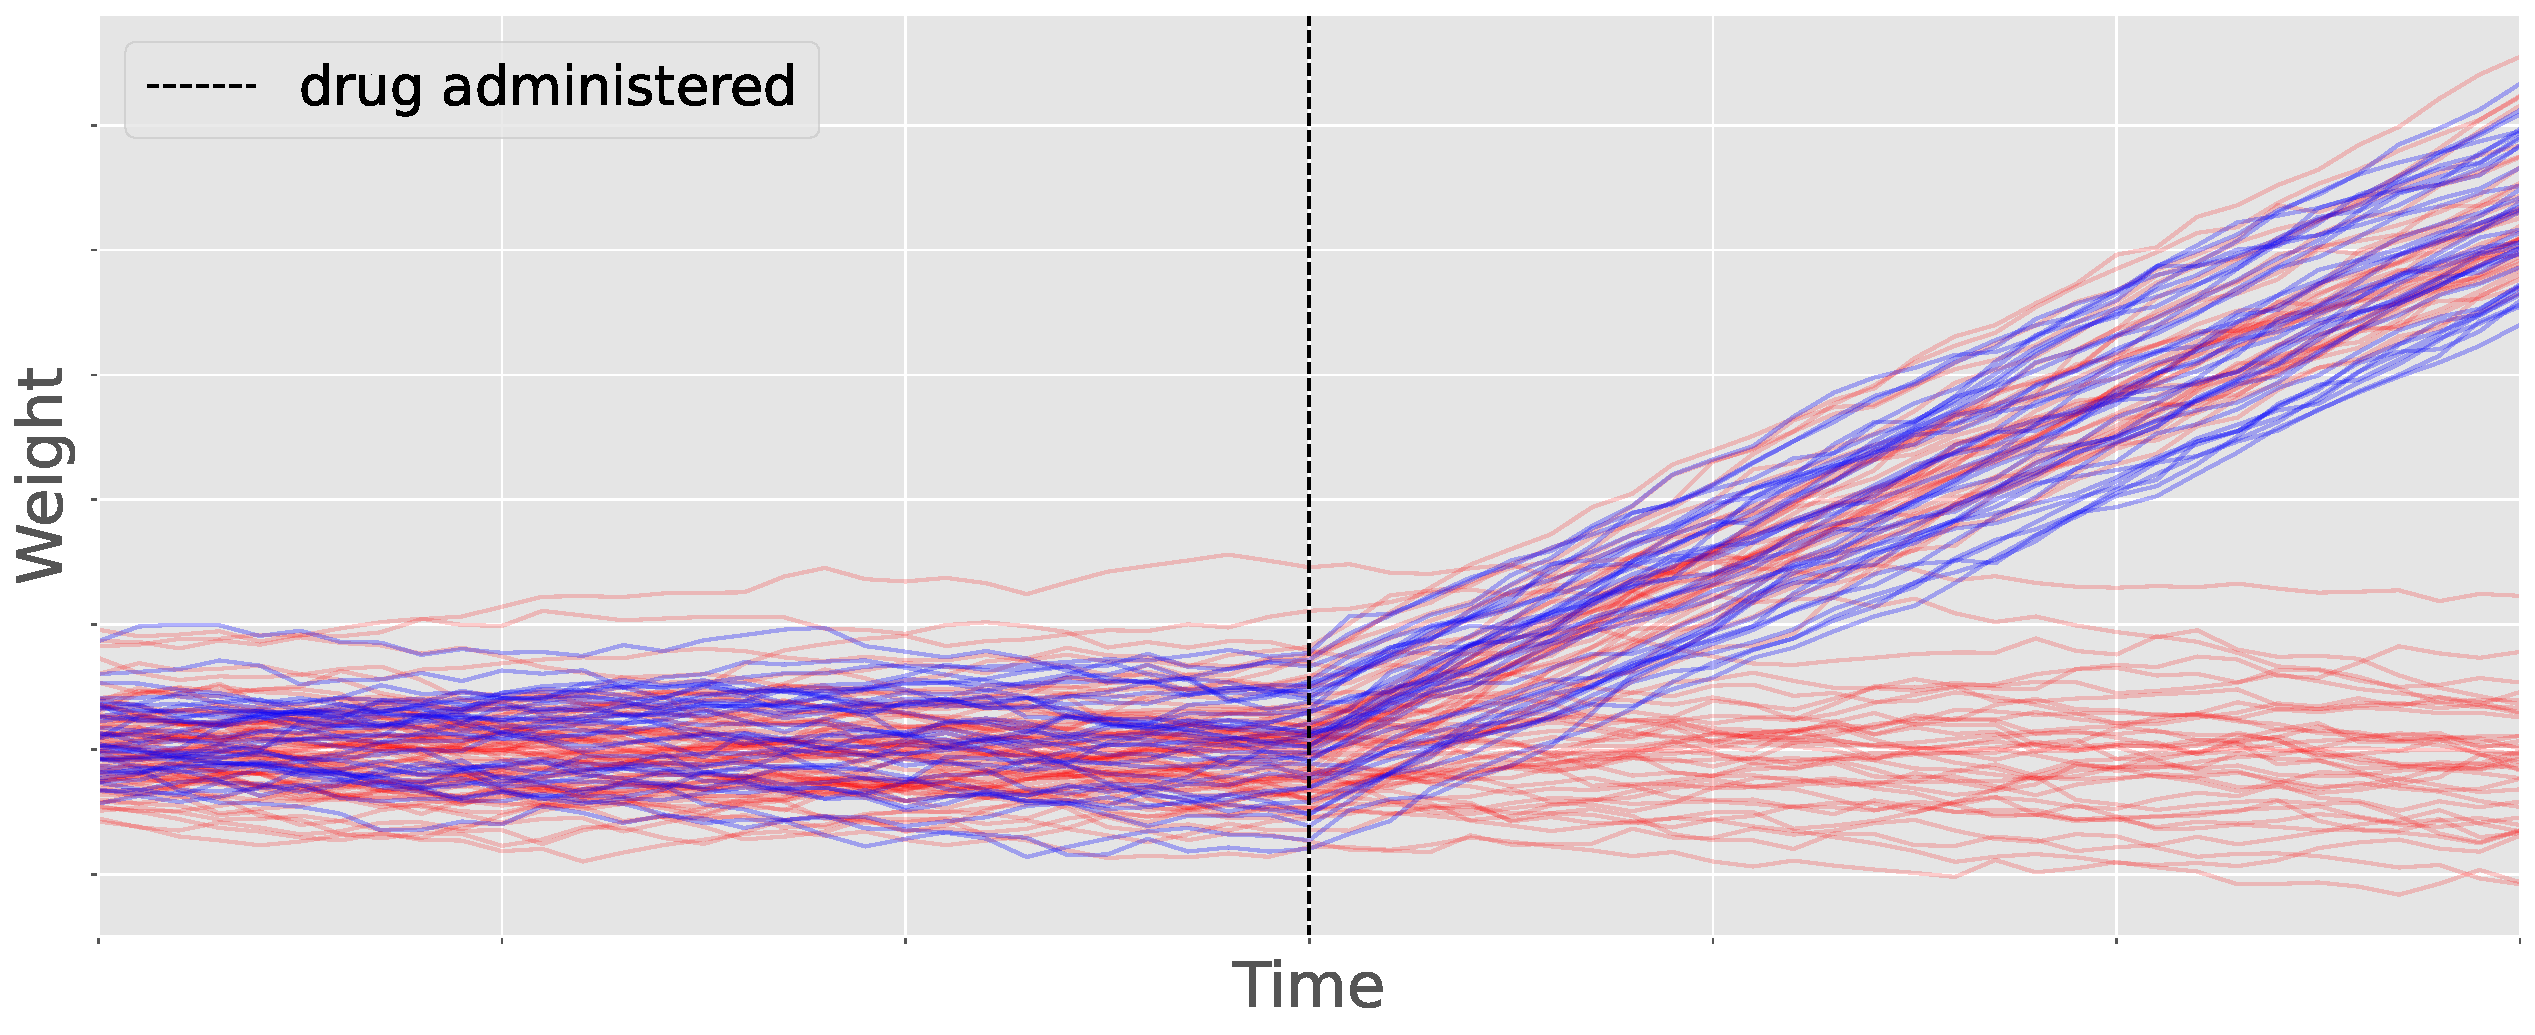
\includegraphics[height=3.3cm]{figures/causal/synthetic_example_newest2.pdf}
    \caption{The discrepancy between observational data and interventional behaviour in the presence of unmeasured confounding: the range of outcomes observed in the data for patients who were administered the drug (blue) differs from what \emph{would} be observed if the drug were administered to the general population (red).}
    \label{fig:syn_ex_intro}
\end{figure}

% \subsection{Causal unidentifiability under unmeasured confounding}\label{subsec:unmeasured-confounding}
% Here, we elaborate further on the implications of unmeasured confounding on the identifiability of causal effects in sequential decision setting. This topic forms the central focus of Chapter \ref{ch:5-causal} of this thesis.
% \paragraph{Observational data}
% Recall that in this setting, our observational data comprises trajectories obtained by observing the interaction of some behavioural agents with the real-world process.
% We model each trajectory as follows.
% First, we represent the action chosen by the agent at time $\tx \in \{1, \ldots, \T\}$ as an $\Aspace_\tx$-valued random variable $\A_\tx$.
% We then obtain a trajectory in our dataset by recording at each step the action $\A_\tx$ chosen and the observation $\X_\tx(\A_{1:\tx})$ corresponding to this choice of action.
% As a result, each observed trajectory has the following form:
% \begin{equation} \label{eq:observed-data-trajectory-intro}
%     \X_0, \A_1, \X_1(\A_1), \ldots, \A_\T, \X_\T(\A_{1:\T}).
% \end{equation}

% Informally, the assumption of no unmeasured confounding holds when each action $\A_\tx$ is chosen by the behavioural agent solely on the basis of the information available at time $\tx$ that is actually recorded in the dataset, namely $\X_{0}, \A_1, \X_1, \ldots, \A_{\tx-1}, \X_{\tx-1}$, as well as possibly some additional randomness that is independent of the real-world process, such as the outcome of a coin toss. Unobserved confounding is present whenever this does not hold, i.e.\ whenever some unmeasured factor simultaneously influences both the agent's choice of action and the observation produced by the real-world process.


In certain contexts it may be reasonable to assume that the data are unconfounded. For example, in certain situations it may be possible to gather data in a way that specifically guarantees there is no confounding.
Randomised controlled trials, which ensure that each $\A_\tx$ is chosen via a carefully designed randomisation procedure \citep{lavori2004dynamic,murphy2005experimental}, constitute a widespread example of this approach. However, for typical datasets, it is widely acknowledged that the assumption of no unmeasured confounding will rarely hold, and so OPE procedures based on this assumption may yield unreliable results in practice \citep{murphy2003optimal,tsiatis2019dynamic}. 
This is formalised in a foundational result from the causal inference literature, often referred to as the \emph{fundamental problem of causal inference} \citep{holland1986statistics}.
% shows that the value for a deterministic target policy (which always chooses a given action sequence $\ax_{1:\tx}$ regardless of the past observations $X_{0:\tx-1}(\ax_{1:\tx-1})$) is unidentifiable.
\begin{mainresultwithtitle}[title=Fundamental problem of causal inference (informal statement)]\noindent
    The causal effect of an action is not uniquely identified by the observational data distribution in the presence of unmeasured confounding (without additional assumptions).
\end{mainresultwithtitle}

% \begin{theorem}\label{thm:unidentifiability-intro}
%     If $\Prob(\A_{1:\tx} \neq \ax_{1:\tx}) > 0$, then the expectation $\E[\X_{\tx}(\ax_{1:\tx})]$ is not uniquely identified by the distribution of the data in \eqref{eq:observed-data-trajectory-intro} without further assumptions.
% \end{theorem}

\paragraph{Partial identification}
Since the precise identifiability of causal effects is not possible in the presence of unmeasured confounding, a notable line of work instead explores partial identification techniques \citep{manski,manski1989anatomy, manski2003partial}. Instead of the point identification of causal effects which may require strong unconfounding assumptions, partial identification typically considers the range of causal effects which may occur in the presence of confounding. For example, \cite{manski} constructs sharp bounds on the causal effects which can be readily estimated using the available observational data. While these bounds do not require any strong assumptions, they can be conservative. 

\paragraph{Sensitivity analysis}
Slightly stronger assumptions yield inferences that may be more powerful but less credible. To this end, \cite{rosenbaum2002observational} proposes a classical model of confounding for a single binary decision setting which posits that the unobserved confounders have a limited influence on the agent's actions in the real world.  \cite{namkoong2020offpolicy} extend this model to the multi-action sequential decision-making setting, and subsequently use this to obtain bounds on the off-policy value.

The Rosenbaum model is also closely related to (albeit different from) the marginal sensitivity model introduced by \cite{tan2006distributional} which also assumes bounds on the strength of unmeasured confounding on agent's actions. Subsequently, \cite{kallus2020minimax} uses the marginal sensitivity model to develop a policy learning algorithm which remains robust to unmeasured confounding. However, these models impose assumptions on the strength of unmeasured confounding which can be impossible to verify using observational data alone, and therefore the inferences obtained may be misleading in many cases. 

\paragraph{Proxy causal learning}
This comprises methodologies for estimating the causal effect of actions on outcomes in the presence of unobserved confounding, using \emph{proxy variables} which contain relevant side information about the unmeasured confounders \citep{xu2021deep, tchetgen2020introduction, xu2024kernel}. This usually involves a two-stage regression. First, the relationship between action and proxies is modelled and subsequently, this model is used to learn the causal effect of actions on the outcomes. \cite{kuroki2014measurement} outline the necessary conditions on proxy variables to obtain the true causal effects. While proxy causal learning may be effective in cases where such proxy variables are available, in many real-world settings the available proxy variables may not satisfy the necessary conditions for identification of true causal effects.

Chapter \ref{ch:5-causal} of this thesis considers the challenges posed by unmeasured confounding in sequential decision setting. We propose a set of novel bounds on the causal effects in this setting, which remain valid in the presence of arbitrary unmeasured confounding and rely on minimal assumptions making them highly applicable to a wide variety of real-world settings. 


% it is straightforward to show that the joint density of $(X, A, Y)$ from which the logged data $\D$ is sampled, denoted by $\pbeh$, can be factorised as follows:
% \begin{align}
%     \pbeh(x, a, y) \coloneqq p(y\mid x, a)\, \textcolor{blue}{\beh(a\mid x)}\,p(x). \label{eq:behav-joint-factorisation-intro}
% \end{align}
% Likewise, the joint density of $(X, A, Y)$ under the \textit{target policy} $\tar$ can be factorised as
% \begin{align}
%     \ptar(x, a, y) \coloneqq p(y\mid x, a)\, \textcolor{red}{\tar(a\mid x)}\,p(x). \label{eq:tar-joint-factorisation-intro}
% \end{align}

% Moreover, we use $\Ebeh$ and $\Etar$ to denote the expectations under the joint densities $\pbeh(x, a, y)$ and $\ptar(x, a, y)$ respectively, i.e.,
% \begin{align*}
%     \Ebeh[\,\cdot\,] \coloneqq \E_{(X, A, Y)\sim \pbeh}[\,\cdot\,], \qquad \textup{and} \qquad \Etar[\,\cdot\,] \coloneqq \E_{(X, A, Y)\sim \ptar}[\,\cdot\,].
% \end{align*}

% \begin{importantresultwithtitle}[title=Off-policy evaluation (OPE)]\noindent
% The main objective of off-policy evaluation (OPE) is to estimate the expectation of the outcome $Y$ under a given target policy $\tar$, i.e., $\Etar [Y]$, using only the logged data $\D$.
% \end{importantresultwithtitle}

% % \todo{include causal formulation and connect it with this}

% % \begin{importantresultwithtitle}[title=Causal formulation]\noindent
% \paragraph{Causal formulation}
%  To make the causal dependence of the action on the outcome explicit, we can reformulate the contextual bandits setting using the \emph{potential outcomes framework} proposed by \cite{robins1986new}. 
%  Here, for a given action $a \in \mathcal{A}$ we denote the random variable $Y(a)$ (also known as the potential outcome), as the outcome that \emph{would} occur if the action $a$ is chosen. As random variables, $Y(a)$ may also depend on the initial covariates $X$ and additional randomness which is not explicitly modelled. Moreover, this notation can be reconciled with the conventional contextual bandits setting above by noting that, in the real world where an agent chooses action $A \in \mathcal{A}$ for context $X$, the outcome $Y$ observed is explicitly expressed as $Y(A)$, i.e. $Y\coloneqq Y(A)$ in the observational data. This corresponds to the standard consistency assumption in causal inference \citep{hernan2020causal} and intuitively means that the potential outcome $Y(a)$ is observed in the data when the agent actually chose $A=a$. 
% % \end{importantresultwithtitle}

% Contextual bandits encapsulate the single-decision regimes where, for each observed context, we take a single action and observe the resulting outcome. This is analogous to a doctor choosing a single treatment for a patient based on their current state. However, many real-world decision-making scenarios involve multiple interventions over time, where each action not only affects the immediate outcome but also influences the context for future decisions. To capture this complexity, we introduce the concept of dynamic treatment regimes (DTRs) \citep{tsiatis2019dynamic} in the following section. DTRs extend the framework of contextual bandits to handle sequential decision-making problems, allowing us to model more complex scenarios where interventions unfold over time and the context evolves dynamically.

% \section{Dynamic treatment regimes}
% We consider a setting with a fixed number of decisions per episode (i.e., a fixed time horizon) $T \in \{1, 2, \ldots\}$. For each $t\in \{0, \ldots, T\}$, we assume that the process gives rise to an observation at time $t$, denoted by $X_t$ which takes values in some space $\mathcal{X}_t \coloneqq \R^{\Xspacedim_\tx}$. 
% % Moreover, the process can be influenced by some action at time $t \in \{1, \ldots, T\}$ which takes values in some space $\mathcal{A}_t$. 
% Moreover, at time $t\in  \{1, \ldots, T\}$ a real-world agent (such as a doctor) chooses an action $A_t$ which takes values in some space $\mathcal{A}_t$. The agent's choice of $A_t$ may depend on the historical observations $(X_0, \ldots, X_{t-1})$ or any additional information not captured in historical observations that the agent can access. For example, in a medical context, the observations may consist of a patient's vital signs, and the actions may consist of possible treatments or interventions that the doctor chooses based on patient history.
% % In the real world, the action at time $t$ may be chosen by an agent (such as a doctor) based on the . 
% The actions taken up till time $t$, i.e. $(A_1, A_2, \ldots, A_t)$ can influence the future observations $(X_t, X_{t+1}, \ldots, X_T)$. 
% This setting describes dynamic treatment regimes, of which the contextual bandits are a special case when $T=1$. 
% % To make this concrete, in a robotics context, the observations may consist of all the readings of all the sensors of the robot, and the actions may consist of commands that can be input by an external user. In a medical context, the observations may consist of the vital signs of a patient, and the actions may consist of possible treatments or interventions. 

% % \begin{importantresultwithtitle}[title=Causal formulation]\noindent
% \paragraph{Causal formulation}
% As before, we make the causal dependence of past actions on future observations explicit by modelling the dynamics of the real-world process via the longitudinal potential outcomes framework proposed \citep{rubin1974estimating,rubin2005causal}. To streamline notation, we will index the spaces using vector notation, so that e.g.\ $\Aspace_{1:t}$ denotes the Cartesian product $\Aspace_1 \times \cdots \times \Aspace_t$, and $a_{1:t} \in \Aspace_{1:t}$ is a choice of $a_1 \in \Aspace_1, \ldots, a_t \in \Aspace_t$.

% In this formulation, for each action sequence $a_{1:T} \in \Aspace_{1:T}$, we posit the existence of random variables or \emph{potential outcomes} $X_0, X_1(a_1), \ldots, X_T(a_{1:T})$, where $X_t(a_{1:t})$ takes values in $\Xspace_t$.
% We will denote this sequence more concisely as $X_{0:T}(a_{1:T})$.
% % Each $\X_\tx(\ax_{1:\tx})$ is referred to as a \emph{potential outcome}.
% Intuitively, $X_0$ represents data available before the first action, while $X_{1:T}(a_{1:T})$ represents the sequence of real-world outcomes that \emph{would} occur if actions $a_{1:T}$ were taken successively.
% These potential outcomes $X_{1:T}(a_{1:T})$ are also referred to as \emph{interventional outcomes} under the intervention $a_{1:T}$.

% As random variables, each $X_{t}(a_{1:t})$ may depend on additional randomness that is not explicitly modelled, and so, in particular, may be influenced by all the previous potential outcomes $X_{0:t-1}(a_{1:t-1})$, and possibly other random quantities.
% This models a process whose initial state is determined by external factors, such as when a patient from some population first presents at a hospital, and where the process then evolves according both to specific actions chosen from $\Aspace_{1:T}$ as well as additional external factors.

% Just like in the contextual bandits setting, this causal notation can be reconciled with the conventional (non-causal) notation above by noting that, in the real world where an agent chooses action $A_{1:t} \in \mathcal{A}_{1:t}$, the observation at time $t$, $X_{t}$, is explicitly expressed as $X_{t}(A_{1:t})$, i.e. $X_{t}\coloneqq X_{t}(A_{1:t})$ in the observational data. Like before, this is the standard consistency assumption in causal inference \citep{hernan2020causal} and intuitively means that the potential outcome $X_{t}(a_{1:t})$ is observed in the data when the agent chose $A_{1:t}=a_{1:t}$. 
% % \end{importantresultwithtitle}


% Now that we have outlined the single and multiple decision frameworks, we are now equipped to formally define the off-policy evaluation setting which is fundamental to the problems considered in this thesis.  

% \section{Off-policy evaluation}
% Off-policy evaluation (OPE) tackles a crucial challenge in decision-making: assessing the performance of a new policy using data collected under a different policy \citep{swaminathan2015counterfactual, wang2017optimal, farajtabar2018more, su2019continuous, metelli2021subgaussian, liu2019triply, sugiyama2012machine, swaminathan2017off}. This is particularly valuable when conducting controlled experiments with the new policy is impractical or unethical. In what follows, we formally define the OPE problem in contextual bandits which will set up the challenges tackled in Chapters \ref{ch:3-mr} and \ref{ch:4-copp} of this thesis. 

% \subsection{Off-policy evaluation in contextual bandits}
% Recall the standard contextual bandit setting, where $X\in\Xspace$ is a context vector (e.g., user features), $A\in \Aspace$ denotes an action (e.g., recommended website to the user), and $Y\in \Yspace$ denotes a scalar reward or outcome (e.g., whether the user clicks on the website). 

% \begin{assumption}[No unmeasured confounding]\label{assum:no-unmeasured-confounding}
% In this setting, it is standard to assume that the agent's action $A$ depends only on the context $X$ and possibly additional randomness independent of everything else. This means that when choosing the action $A$, the agent does not rely on additional information relevant to the outcome $Y$ which is not captured in the context $X$. To be concrete, in a medical context, this assumption means that all of the information that clinicians use to make treatment decisions is captured in the data. This assumption is also referred to as the \emph{strong ignorability assumption} \citep{tsiatis2019dynamic} and can be technically outlined in the language of potential outcomes as follows:
%     \begin{align*}
%         \{Y(a) \, | \, a \in \Aspace\} \indep A \mid X
%     \end{align*}
% \end{assumption}

% % Under Assumption \ref{assum:no-unmeasured-confounding}, we assume that the outcome and context are sampled from unknown probability distributions $p(y\mid x, a)$ and $p(x)$ respectively. 
% Let $\D\coloneqq \{(x_i, a_i, y_i)\}_{i=1}^n$ be a historically logged dataset with $n$ observations, generated by a (possibly unknown) \emph{behaviour policy} $\beh(a\mid x)$, i.e. the conditional distribution of agent's actions is $A\mid X=x \sim \beh(\,\cdot\mid x)$.
% Then, under Assumption \ref{assum:no-unmeasured-confounding}, it is straightforward to show that the joint density of $(X, A, Y)$ from which the logged data $\D$ is sampled, denoted by $\pbeh$, can be factorised as follows:
% \begin{align}
%     \pbeh(x, a, y) \coloneqq p(y\mid x, a)\, \textcolor{blue}{\beh(a\mid x)}\,p(x). \label{eq:behav-joint-factorisation-intro}
% \end{align}
% Likewise, the joint density of $(X, A, Y)$ under the \textit{target policy} $\tar$ can be factorised as
% \begin{align}
%     \ptar(x, a, y) \coloneqq p(y\mid x, a)\, \textcolor{red}{\tar(a\mid x)}\,p(x). \label{eq:tar-joint-factorisation-intro}
% \end{align}

% Moreover, we use $\Ebeh$ and $\Etar$ to denote the expectations under the joint densities $\pbeh(x, a, y)$ and $\ptar(x, a, y)$ respectively, i.e.,
% \begin{align*}
%     \Ebeh[\,\cdot\,] \coloneqq \E_{(X, A, Y)\sim \pbeh}[\,\cdot\,], \qquad \textup{and} \qquad \Etar[\,\cdot\,] \coloneqq \E_{(X, A, Y)\sim \ptar}[\,\cdot\,].
% \end{align*}

% \begin{importantresultwithtitle}[title=Off-policy evaluation (OPE)]\noindent
% The main objective of off-policy evaluation (OPE) is to estimate the expectation of the outcome $Y$ under a given target policy $\tar$, i.e., $\Etar [Y]$, using only the logged data $\D$.
% \end{importantresultwithtitle}

% \subsubsection{Existing off-policy evaluation methodologies}
% Next, we will present some of the most commonly used OPE estimators before outlining the limitations of these methodologies. 
% This motivates our proposal presented in Chapter \ref*{ch:3-mr} of this thesis. 

% The value of the target policy can be expressed as the expectation of outcome $Y$ under the target data distribution $\ptar(x, a, y)$.
% % The policy value of target policy $\tar$ can be written as:
% % \[
% % \Etar[Y] = \int_{\Xspace, \Aspace, \Yspace} y\, \ptar(x, a, y) \, \mathrm{d}x \, \mathrm{d}a \, \mathrm{d}y.
% % \]
% However in most cases, we do not have access to samples from this target distribution and hence we have to resort to importance sampling methods.
% \paragraph{Inverse Probability Weighting (IPW) estimator}
% One way to compute the target policy value, $\Etar[Y]$, when only given data generated from $\pbeh(x, a, y)$ is to rewrite the policy value as follows:
% % _{\Xspace, \Aspace, \Yspace}

% \begin{small}
% \begin{align*}
%     \Etarred[Y] =
%     \int y \, \ptar(x, a, y) \,\mathrm{d}y \, \mathrm{d}a\, \mathrm{d}x   =
%     \int y \, \underbrace{\frac{\ptar(x, a, y)}{\pbeh(x, a, y)}}_{\rho(a,x)}\, \pbeh(x, a, y) \,\mathrm{d}y \, \mathrm{d}a\, \mathrm{d}x =
%     % \Ebehblue\left[Y\,\frac{\ptar(X, A, Y)}{\pbeh(X, A, Y)} \right] = 
%     \Ebehblue\left[Y\,\rho(A, X)\right],
% \end{align*}
% \end{small}
% where 
% $
% \rho(a, x) \coloneqq \frac{\ptar(x, a, y)}{\pbeh(x, a, y)} = \frac{\tar(a|x)}{\beh(a|x)}
% $, given the factorizations in Eqns. \eqref{eq:behav-joint-factorisation-intro} and \eqref{eq:tar-joint-factorisation-intro}.
% This leads to the commonly used \emph{Inverse Probability Weighting (IPW)} \citep{horvitz1952generalization} estimator:
% \[
% \thetaipw \coloneqq \frac{1}{n}\sum_{i=1}^n \rho(a_i, x_i)\,y_i.
% \]
% When the behaviour policy is known, IPW is an unbiased and consistent estimator. However, it can suffer from high variance, especially as the overlap between the behaviour and target policies decreases. 

% \paragraph{Doubly Robust (DR) estimator} 
% To alleviate the high variance of IPW, \cite{dudik2014doubly} proposed a \emph{Doubly Robust (DR)} estimator for OPE. 
% DR uses an estimate of the conditional mean $\hat{\mu}(a, x) \approx\E[Y\mid X=x, A=a]$ (\emph{outcome model}), as a control variate to decrease the variance of IPW. It is also doubly robust in that it yields accurate value estimates if either the importance weights $\rho(a, x)$ or the outcome model $\hat{\mu}(a, x)$ is well estimated \citep{dudik2014doubly, jiang2016doubly}. 
% The DR estimator for $\Etar[Y]$ can be written as follows:
% \[
% \thetadr = \frac{1}{n} \sum_{i=1}^n \rho(a_i, x_i)\,(y_i - \hat{\mu}(a_i, x_i)) + \hat{\eta}(\tar),
% % \vspace{-0.7mm}
% \]
% where
% \begin{align}
%     \hat{\eta}(\tar) = \frac{1}{n} \sum_{i=1}^n \sum_{a'\in \Aspace} \hat{\mu}(a', x_i) \tar(a'\mid x_i) \approx \E_{\tar}[\hat{\mu}(A, X)]. \label{eq:direct-method-intro}
% \end{align}
% Here, $\hat{\eta}(\tar)$ is referred to as the Direct Method (DM) as it uses $\hat{\mu}(a, x)$ directly to estimate target policy value. 


% % \subsection{OPE in dynamic treatment regimes}
% % - maybe skip this

% \section{Limitations of existing OPE methods}
% \subsection{High variance}\label{subsec:high-variance}
% The conventional off-policy value estimators (including IPW and DR estimators) use policy ratios $\rho(a, x) \coloneqq \tar(a\mid x)/\beh(a\mid x)$ as importance weights. 
% In cases where the two policies are significantly different, the policy ratios $\rho(a, x)$ attain extreme values leading to a high variance in the OPE estimators. 
% Even though the DR estimator uses control variates for variance reduction, it still relies on policy ratios as importance weights and as a result, also suffers from high variance when the policy shift is large. 
% This problem is further exacerbated as the sizes of the action and context spaces grow \citep{sachdeva2020off, saito2022off}.
% Chapter \ref{ch:3-mr} of this thesis specifically focuses on this limitation of OPE. 

% Besides using control variates (as in DR estimator), several techniques have been proposed to address the variance issues associated with importance weights. 


% \paragraph{Weight clipping and normalization}
% \cite{swaminathan2015counterfactual, swaminathan2015the, chaudhuri2019london} attempt to bound the importance weights within a certain range to prevent them from becoming excessively large. However, these approaches introduce a bias-variance trade-off, as clipping the weights can introduce bias into the estimates. Similarly, Switch-DR \citep{wang2017optimal} aims to circumvent the high variance in conventional DR estimator by switching to the Direct Method when the importance weights are large:
% \[
% \thetaswitch \coloneqq \frac{1}{n} \sum_{i=1}^n \rho(a_i, x_i)\,(y_i - \hat{\mu}(a_i, x_i))\ind(\rho(a_i, x_i) \leq \tau) + \hat{\eta}(\tar),
% \]
% where $\tau \geq 0$ is a hyperparameter, $\hat{\mu}(a, x) \approx \E[Y \mid X=x, A=a]$ is the outcome model, and $\hat{\eta}$ is the Direct Method (DM) as defined in \eqref{eq:direct-method-intro}.
% Like weight clipping, this approach can also increase the bias, since the DM can have a high bias.


% \paragraph{Marginalization-based techniques}
% Several works explore marginalisation techniques for variance reductions. For example, \cite{saito2022off} propose MIPS, which considers the marginal shift in the distribution of a lower dimensional embedding of the action space, denoted by $E$, instead of considering the shift in the policies explicitly (as in IPW). 
% While this approach reduces the variance associated with IPW, we show in Chapter \ref{ch:3-mr} that MIPS relies on an additional assumption regarding the action embeddings $E$ which does not hold in general.

% In addition, various marginalisation ideas have also been proposed in the context of reinforcement learning (RL). For example, \cite{liu2018breaking, xie2019advances, kallus2020off} use methods which consider the shift in the marginal distribution of the states, and apply importance weighting with respect to this marginal shift rather than the trajectory distribution. Similarly, \cite{Fujimoto2021deep} use marginalisation for OPE in deep RL, where the goal is to consider the shift in marginal distributions of state and action. Although marginalization is a key trick of these estimators, these techniques are aimed at resolving the curse of horizon, a problem specific to RL.



% \subsection{Lack of uncertainty quantification}\label{subsec:uncertainty-quantification}
% Most techniques for OPE in contextual bandits focus on evaluating policies based on their \emph{expected} outcomes \citep{uncertainty5, adaptive-ope, uncertainty2, uncertainty3, uncertainty4, doubly-robust}. However, this can be problematic as
% methods that are only concerned with the average outcome do not take into account any notions of
% variance, for example. Therefore, in risk-sensitive settings such as econometrics, where we want
% to minimize the potential risks, metrics such as CVaR (Conditional Value at Risk) might be more
% appropriate \citep{keramati2020being}. Additionally, when only small sample sizes of observational data are available, the average outcomes under finite data can be misleading, as they are prone to outliers and hence, metrics such as medians or quantiles are more robust in these scenarios \citep{altschuler2019best}. Next, we outline some recent works which tackle this challenge by developing methodologies to account for the uncertainty in off-policy performance using available data. 

% \paragraph{Off-policy risk assessment in contextual bandits}
% Instead of estimating bounds on the expected outcomes, \cite{risk-assessment, chandak2021universal} establish finite-sample bounds for a general class of metrics (e.g., Mean, CVaR, CDF) on the outcome. Their methods can be used to estimate quantiles of the outcomes under the target policy and are therefore robust to outliers. 

% For example, given observational dataset $\D = \{(x_i, a_i, y_i)\}_{i=1}^{n}$, \cite{chandak2021universal} proposed a non-parametric Weighted Importance Sampling (WIS) estimator for the empirical CDF of $Y$ under $\pi^*$, 
% $$
% \hat{F}_{\textup{WIS}}(t) \coloneqq \frac{\sum_{i=1}^{n} \hat{\rho}(a_i, x_i) \mathbbm{1}(y_i \leq t)}{\sum_{i=1}^{n} \hat{\rho}(a_i, x_i)}
% $$
% where $\hat{\rho}(a, x) \coloneqq \frac{\pi^*(a \mid x)}{\hat{\pi}^b(a \mid x)}$ are the importance weights. \cite{chandak2021universal} show that $\hat{F}_{\textup{WIS}}(t)$ is a uniformly consistent estimator of the off-policy CDF, $F_{\tar}(t) \coloneqq \p_{\tar}(Y \leq t)$.
% Therefore, we can use $\hat{F}_{\textup{WIS}}$ to construct predictive intervals on the outcome $Y$ under target policy $\tar$. This can help us quantify the range of plausible outcomes $Y$ that are likely to occur if actions are chosen according to target policy $\tar$. However, the resulting bounds do not depend on the context $X$ (i.e., are not adaptive w.r.t. $X$). This can lead to overly conservative intervals, which may not be very informative. In Chapter \ref{ch:4-copp}, we circumvent this problem by proposing a methodology of constructing predictive intervals on $Y$ under target policy $\tar$ which are adaptive w.r.t. context $X$ and are therefore considerably more informative.


% \subsection{Assumption of no unmeasured confounding}\label{subsec:unmeasured-confounding}
% The standard OPE methodologies assume no unmeasured confounding (formalised in Assumption \ref{assum:no-unmeasured-confounding}) in the available observational data. This assumption is unverifiable from the observational data alone and is violated in many real-world circumstances where some information not captured in the data influences not only the action $A$ chosen, but also the outcome $Y$ observed subsequently. This can happen when the real-world agent has access to more information than is available in the context $X$ captured in the data. 
% In such circumstances, the causal effect of a given action $a \in \Aspace$ may be unidentifiable from the available observational data, making it impossible to accurately estimate the value of the target policy.
% To make this concrete, we provide an intuitive illustration of this phenomenon below using a toy example where the available observational suffers from unmeasured confounding.

% \begin{figure}[t]
%     \centering
%     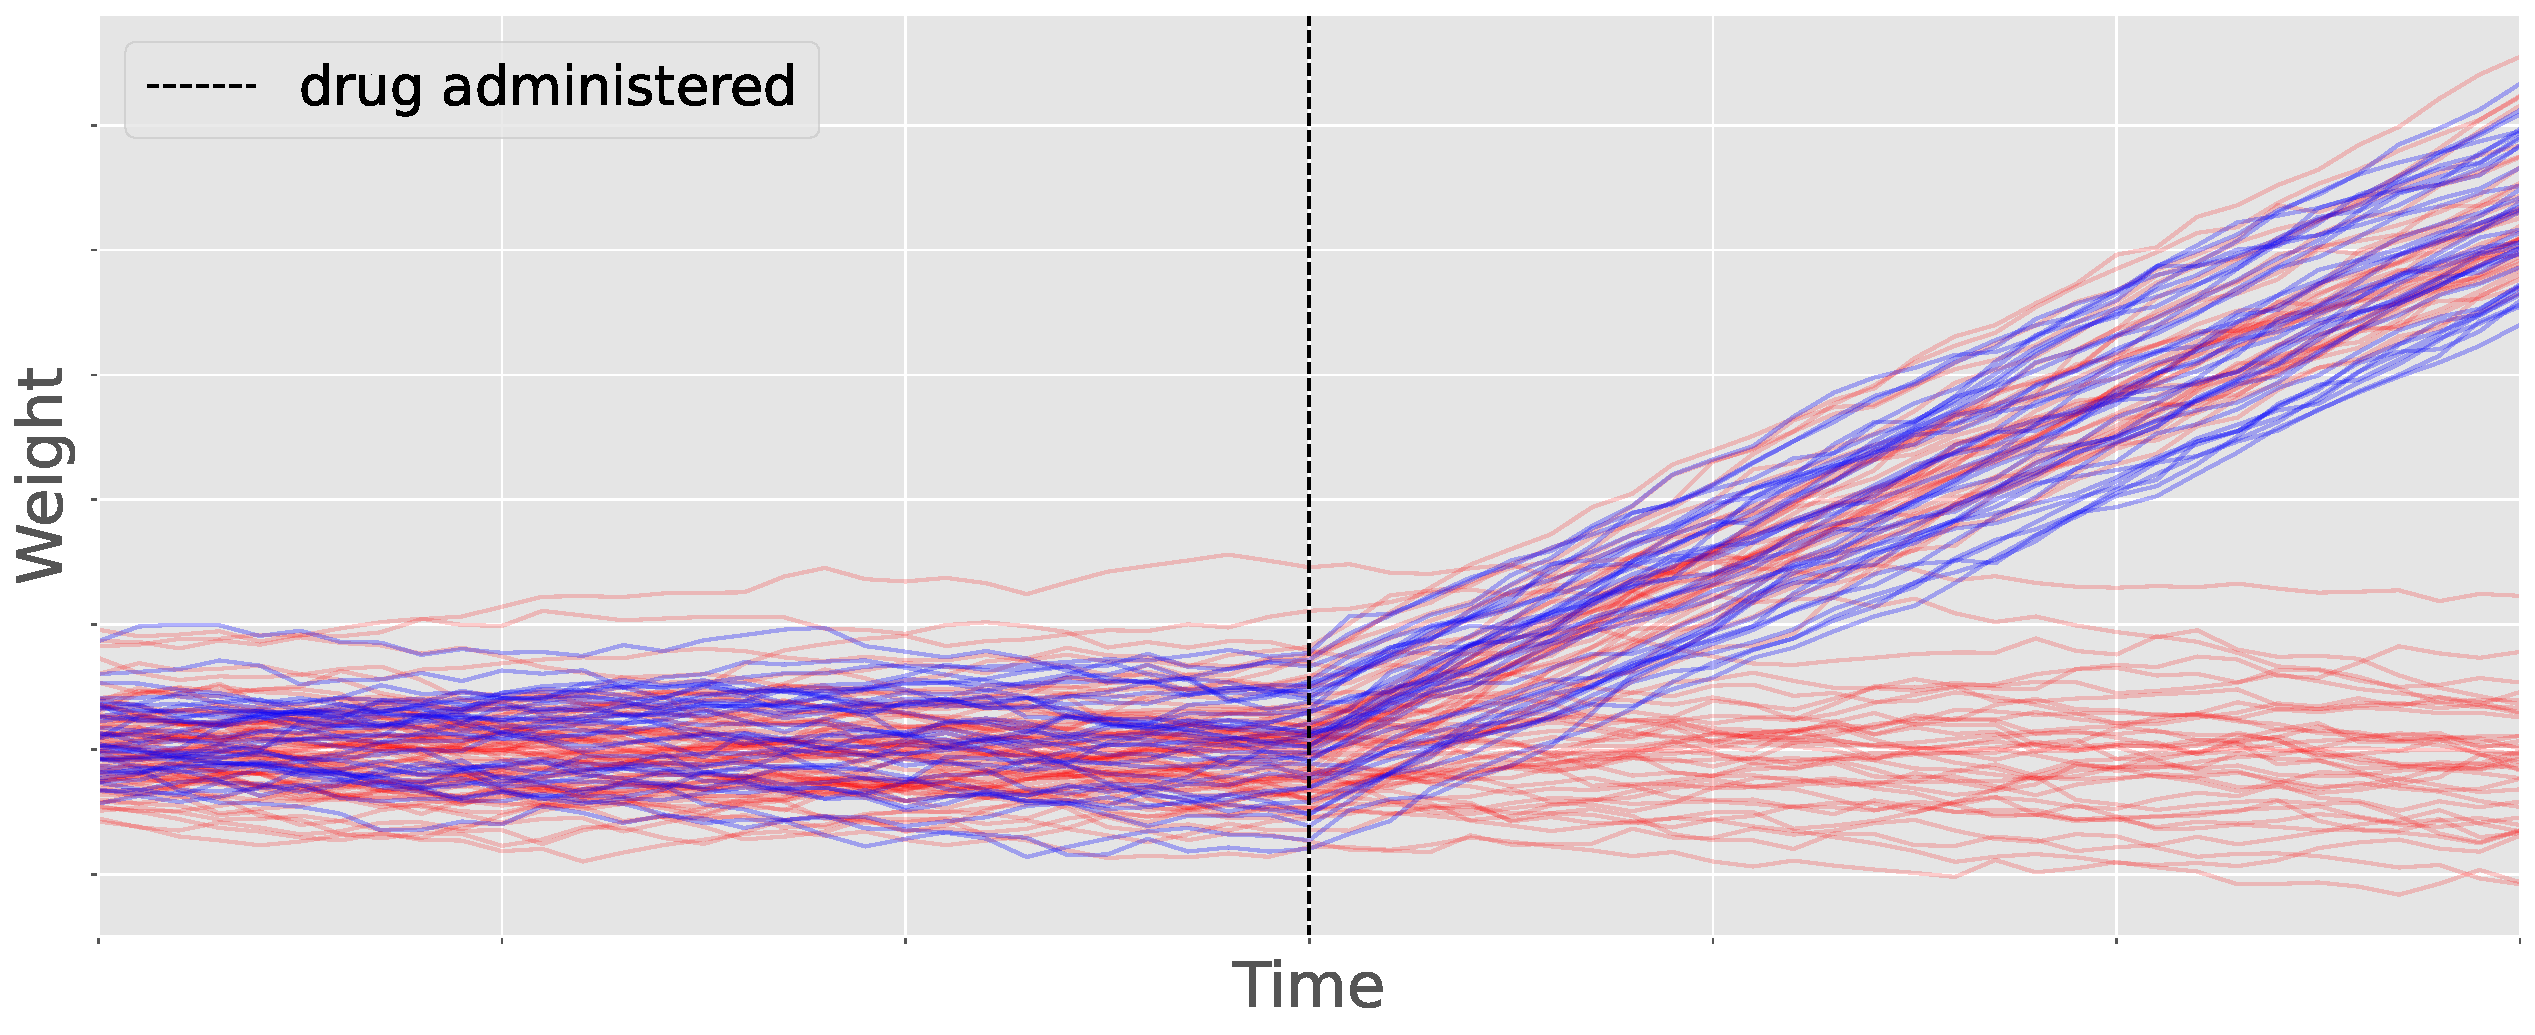
\includegraphics[height=3.3cm]{figures/causal/synthetic_example_newest2.pdf}
%     \caption{The discrepancy between observational data and interventional behaviour in the presence of unmeasured confounding: the range of outcomes observed in the data for patients who were administered the drug (blue) differs from what \emph{would} be observed if the drug were administered to the general population (red).}
%     \label{fig:syn_ex_intro}
% \end{figure}

% \begin{importantresultwithtitle}[title=Toy example: Unmeasured confounding in medical decision-making]\noindent
% Suppose that we are interested in estimating the effect of a drug on the weight of patients in a certain population. 
% Moreover, assume that this drug interacts with an enzyme that is only present in part of the population.
% Denote by $U \in \{0, 1\}$ the presence or absence of the enzyme in a patient, and assume that when $U = 1$ the patient's weight increases after action the drug is administered, and that when $U = 0$ the drug has no effect.
% Additionally, suppose that, among the patients whose data we have obtained, the drug was only prescribed to those for whom $U = 1$, perhaps on the basis of some initial lab reports available to the prescriber.
% Finally, suppose that these lab results were \emph{not} included in the context $X$ captured in the observational dataset $\D$, so that the value of $U$ for each patient cannot be determined from the data we have available. 

% In this setup, since the drug was only administered to patients with $U=1$, it would appear from the data that the drug causes patient weight to increase. 
% However, when the drug is administered to the general population, i.e.\ regardless of the value of $U$, we would observe that the drug has no effect on patients for whom $U=0$. Figure \ref{fig:syn_ex_intro} illustrates this discrepancy under a toy model for
% this scenario. In this example, since the data $\D$ contains no information about the presence or absence of the enzyme in patients, $U$, it is impossible to determine using the data $\D$ alone how the drug will affect a given population of patients. 

% % Consider a medical decision-making scenario where the physician decides whether or not to administer a specific drug to the patients, and the outcome $Y$ corresponds to 
    
% \end{importantresultwithtitle}


% \subsubsection{Causal considerations under unmeasured confounding}
% Here, we elaborate further on the implications of unmeasured confounding on the identifiability of causal effects in dynamic treatment regimes (DTRs). This topic forms the central focus of Chapter \ref{ch:5-causal} of this thesis.

% \paragraph{Observational data}
% Recall that in this setting, our observational data comprises trajectories obtained by observing the interaction of some behavioural agents with the real-world process.
% We model each trajectory as follows.
% First, we represent the action chosen by the agent at time $\tx \in \{1, \ldots, \T\}$ as an $\Aspace_\tx$-valued random variable $\A_\tx$.
% We then obtain a trajectory in our dataset by recording at each step the action $\A_\tx$ chosen and the observation $\X_\tx(\A_{1:\tx})$ corresponding to this choice of action.
% As a result, each observed trajectory has the following form:
% \begin{equation} \label{eq:observed-data-trajectory-intro}
%     \X_0, \A_1, \X_1(\A_1), \ldots, \A_\T, \X_\T(\A_{1:\T}).
% \end{equation}
% As outlined in the previous section, the standard off-policy evaluation methods, both in contextual bandits and DTRs, assume no unmeasured confounding in the observational dataset. Informally, this assumption holds when each action $\A_\tx$ is chosen by the behavioural agent solely on the basis of the information available at time $\tx$ that is actually recorded in the dataset, namely $\X_{0}, \A_1, \X_1(\A_1), \ldots, \A_{\tx-1}, \X_{\tx-1}(\A_{1:\tx-1})$, as well as possibly some additional randomness that is independent of the real-world process, such as the outcome of a coin toss. Unobserved confounding is present whenever this does not hold, i.e.\ whenever some unmeasured factor simultaneously influences both the agent's choice of action and the observation produced by the real-world process.


% While it may be reasonable to assume that the data are unconfounded in certain contexts. For example, in certain situations it may be possible to gather data in a way that specifically guarantees there is no confounding.
% Randomised controlled trials, which ensure that each $\A_\tx$ is chosen via a carefully designed randomisation procedure \citep{lavori2004dynamic,murphy2005experimental}, constitute a widespread example of this approach. However, for typical datasets, it is widely acknowledged that the assumption of no unmeasured confounding will rarely hold, and so OPE procedures based on this assumption may yield unreliable results in practice \citep{murphy2003optimal,tsiatis2019dynamic}. The following foundational result from the causal inference literature (often referred to as the \emph{fundamental problem of causal inference} \citep{holland1986statistics}) formalises this.
% % shows that the value for a deterministic target policy (which always chooses a given action sequence $\ax_{1:\tx}$ regardless of the past observations $X_{0:\tx-1}(\ax_{1:\tx-1})$) is unidentifiable.
% \begin{theorem}\label{thm:unidentifiability-intro}
%     If $\Prob(\A_{1:\tx} \neq \ax_{1:\tx}) > 0$, then the expectation $\E[\X_{\tx}(\ax_{1:\tx})]$ is not uniquely identified by the distribution of the data in \eqref{eq:observed-data-trajectory-intro} without further assumptions.
% \end{theorem}

% The expectation $\E[\X_{\tx}(\ax_{1:\tx})]$ in Theorem \ref{thm:unidentifiability-intro} denotes the value at time $t$ of a deterministic target policy, which always chooses a given action sequence $\ax_{1:\tx}$ regardless of everything else.
% Therefore, this result shows that the value of a deterministic target policy is unidentifiable in general, even if we have access to an infinitely large observational dataset. This also implies that the distribution of outcomes under this deterministic target policy, $\Law[X_{0:\tx}(\ax_{1:\tx})]$, is unidentifiable from the observational data distribution in general. We can also derive an analogous result for general target policies which choose actions at time $t'\in \{1, \ldots, \tx\}$ dynamically depending on past observations \citep{tsiatis2019dynamic}. 

% \paragraph{Partial identification}
% Since the precise identifiability of causal effects is not possible in the presence of unmeasured confounding, a notable line of work instead explores partial identification techniques \citep{manski,manski1989anatomy, manski2003partial}. Instead of the point identification of causal effects which may require strong unconfounding assumptions, partial identification typically considers the range of causal effects which may occur in the presence of confounding. For example, \cite{manski} constructs sharp bounds on the causal effects which can be readily estimated using the available observational data. While these bounds do not require any strong assumptions, they can be conservative. 

% \paragraph{Sensitivity analysis}
% Slightly stronger assumptions yield inferences that may be more powerful but less credible. To this end, \cite{rosenbaum2002observational} proposes a classical model of confounding for a single binary decision setting which posits that the unobserved confounders have a limited influence on the agent's actions in the real world.  \cite{namkoong2020offpolicy} extend this model to the multi-action sequential decision-making setting, and subsequently use this to obtain bounds on the off-policy value.

% The Rosenbaum model is also closely related to (albeit different from) the marginal sensitivity model introduced by \cite{tan2006distributional} which also assumes bounds on the strength of unmeasured confounding on agent's actions. Subsequently, \cite{kallus2020minimax} uses the marginal sensitivity model to develop a policy learning algorithm which remains robust to unmeasured confounding. However, these models impose assumptions on the strength of unmeasured confounding which can be impossible to verify using observational data alone, and therefore the inferences obtained may be misleading in many cases. 

% \paragraph{Proxy causal learning}
% This comprises methodologies for estimating the causal effect of actions on outcomes in the presence of unobserved confounding, using \emph{proxy variables} which contain relevant side information about the unmeasured confounders \citep{xu2021deep, tchetgen2020introduction, xu2024kernel}. This usually involves a two-stage regression. First, the relationship between action and proxies is modelled and subsequently, this model is used to learn the causal effect of actions on the outcomes. \cite{kuroki2014measurement} outline the necessary conditions on proxy variables to obtain the true causal effects. While proxy causal learning may be effective in cases where such proxy variables are available, in many real-world settings the available proxy variables may not satisfy the necessary conditions for identification of true causal effects.

% Chapter \ref{ch:5-causal} of this thesis considers the challenges posed by unmeasured confounding in dynamic treatment regimes. We propose a set of novel bounds on the causal effects in sequential decision-making settings, which remain valid in the presence of arbitrary unmeasured confounding and rely on minimal assumptions making them highly applicable to a wide variety of real-world settings. 


% Under these confounding assumptions, we can obtain bounds on the off-policy value
% When the influence of unobserved confounding on each action is limited

% (Nonparametric Bounds on Treatment Effects)

% (PARTIAL IDENTIFICATION OF PROBABILITY DISTRIBUTIONS)

% - partial identification using proxy variables

% (Partial Identification of Causal Effects Using Proxy Variables)


% (Rosenbaum's model)

% (Nathan kallus's work)

% (emma bronstein)


% \paragraph{Proxy causal learning}

% (An Introduction to Proximal Causal Learning)

% Deep Proxy Causal Learning and its Application to
% Confounded Bandit Policy Evaluation

% - use stuff from the intro here

% Kernel Single Proxy Control for Deterministic Confounding






% \paragraph{Inferring confounders from available data}

% - Causal Effect Inference with Deep Latent-Variable Models

% - 


% - explain unmeasured confounding at an intuitive level\\
% - technical definition of unmeasured confounding\\
% - distribution of Xt and the off-policy value is unidentifiable under unmeasured confounding (also include the motivating example)\\
% - fundamental theorem of causal inference\\
% - Partial identification under unmeasured confounding\\
% - Falsification of interventional regimes using partial identification

\section{Contributions and thesis outline}
Having outlined some of the key challenges associated with off-policy evaluation, we dedicate the rest of this thesis to addressing each of these individually.
Specifically, this thesis is organised as follows:

\paragraph*{Chapter \ref*{ch:3-mr}: Variance reduction \citep{taufiq2023marginal}}
The first challenge we consider is that of high variance in existing OPE estimators based on importance sampling. 
As we mentioned in Section \ref{subsec:high-variance}, this variance is exacerbated in cases where there is low overlap between behaviour and target policies, or where the action or context space is high-dimensional.
To address this challenge, we propose a novel OPE estimator for contextual bandits, the Marginal Ratio (MR) estimator, which uses a marginalisation technique to focus on the shift in the marginal distribution of outcomes $Y$
directly, instead of the policies themselves. 
Unlike the conventional approaches like IPW and DR estimators, intuitively our proposed estimator treats actions $A$ and contexts $X$ as latent variables.
As a result, the resulting estimator is significantly more robust to the overlap between policies and the sizes of action and/or context spaces.
This chapter also includes extensive theoretical and empirical analyses demonstrating the benefits of the MR estimator compared to the state-of-the-art OPE estimators for contextual bandits.
% We further illustrate the utility of the MR estimator in causal inference settings, where it exhibits enhanced performance in estimating Average Treatment Effects (ATE).

% Through rigorous theoretical analysis, we demonstrate the benefits of the MR estimator compared to conventional methods like IPW and DR in terms of variance reduction. 
% Additionally, we establish a connection between the MR estimator and the state-of-the-art Marginalized Inverse Propensity Score (MIPS) estimator, proving that MR achieves lower variance among a generalized family of MIPS estimators. We further illustrate the utility of the MR estimator in causal inference settings, where it exhibits enhanced performance in estimating Average Treatment Effects (ATE).

\paragraph*{Chapter \ref*{ch:4-copp}: Uncertainty quantification \citep{taufiq2022conformal}}
As explained in Section \ref{subsec:uncertainty-quantification}, most OPE methods have focused on the expected outcome of a policy which does not capture the variability of the outcome $Y$.
In addition, many of these methods provide only asymptotic guarantees of validity at best. 
In this chapter, we address these limitations by considering a novel application of conformal prediction \citep{vovk2005algorithmic} to contextual bandits. 
Given data collected under a behavioral policy, we propose \emph{conformal off-policy prediction} (COPP), which can output reliable predictive intervals for the outcome under a new target policy. We provide theoretical finite-sample guarantees without making any additional assumptions beyond the standard contextual bandit setup, and empirically demonstrate the utility of COPP compared with existing methods on synthetic and real-world data.

\paragraph*{Chapter \ref*{ch:5-causal}: Causal considerations \citep{cornish2023causalfalsificationdigitaltwins}}
In this chapter we consider the sequential decision setting, where the available observational data may suffer from unmeasured confounding. 
As mentioned in Section \ref{subsec:unmeasured-confounding}, fundamental results from causal inference mean that in this setting the causal effect of interventions is unidentifiable from the observational distribution.  
To address this challenge, we provide a novel set of longitudinal causal bounds that remain valid under arbitrary unmeasured confounding.

Chapter \ref*{ch:5-causal} focuses on the application of these 
% We apply these 
bounds for assessing the accuracy of \emph{digital twin models}.
These models are virtual systems designed to predict how a real-world process will evolve in response to interventions. 
To be considered accurate, these models must correctly capture the true causal effects of interventions.
Unfortunately, the causal unidentifiability results mean that observational data cannot be used to certify a twin in this sense if the data are confounded.
To circumvent this, we instead use our proposed causal bounds to find situations in which the twin \emph{is not} correct, and present a general-purpose statistical procedure for doing so.
Our approach yields reliable and actionable information about the twin under only the assumption of an i.i.d.\ dataset of observational trajectories, and remains sound even if the data are confounded.

% These bounds can be used to find the worst-case off-policy value 
% These bounds generalize the classical bounds of \cite{manski}, and can be considerably more informative in comparison.
% These bounds can be used to assess whe

\paragraph*{Chapter \ref*{ch:6-conclusion}: Conclusion} 
Finally, we conclude by summarising the main findings of the works presented in this thesis. 
In this chapter, we also discuss some of the limitations of our proposed methodologies and mention some interesting avenues for future research arising from these works. 

\section{An overview of work conducted during the DPhil}
In this section, we provide an overview of the research conducted during the doctoral studies by listing the papers which are included in this thesis, as well those which have been omitted.

\subsection{Works included in the thesis}
Each chapter of this thesis is based on a paper. These papers are listed in chronological order here for completeness.
\begin{enumerate}
    \item \textbf{Muhammad Faaiz Taufiq}*, Jean-Francois Ton*, Rob Cornish, Yee Whye Teh, and Arnaud Doucet.
    Conformal Off-Policy Prediction in Contextual Bandits. In \textit{\textcolor{purple}{Advances in Neural Information Processing
    Systems, 2022}}. \citep{taufiq2022conformal}
    \item Rob Cornish*, \textbf{Muhammad Faaiz Taufiq}*, Arnaud Doucet, and Chris Holmes. Causal Falsification
    of Digital Twins, 2023. \textit{Preprint}. \citep{cornish2023causalfalsificationdigitaltwins}
    \item \textbf{Muhammad Faaiz Taufiq}, Arnaud Doucet, Rob Cornish, and Jean-Francois Ton. Marginal Density Ratio for Off-Policy Evaluation in Contextual Bandits. In 
    \textit{\textcolor{purple}{Advances in Neural Information Processing Systems, 2023}}. \citep{taufiq2023marginal}
\end{enumerate}

\subsection{Works omitted from the thesis}
For the purposes of coherence and conciseness, several works which were part of the doctoral research have been ommitted from this thesis. 
Here, we list these papers along with a brief description in chronological order for completeness. 
\begin{enumerate}
    \item \textbf{Muhammad Faaiz Taufiq}, Patrick Blöbaum, and Lenon Minorics. Manifold Restricted
    Interventional Shapley Values. In \textit{\textcolor{purple}{International Conference on Artificial Intelligence and
    Statistics, 2023}}.  \citep{taufiq2023manifold}
    \item  \textbf{Muhammad Faaiz Taufiq}, Jean-Francois Ton, and Yang Liu. Achievable Fairness on your Data
    with Utility Guarantees. \textit{Preprint}. \citep{taufiq2024achievablefairnessdatautility}
    \item Yang Liu, Yuanshun Yao, Jean-Francois Ton, Xiaoying Zhang, Ruocheng Guo, Hao Cheng, Yegor
    Klochkov, \textbf{Muhammad Faaiz Taufiq}, and Hang Li. 
    Trustworthy LLMs: A Survey and Guideline for Evaluating Large Language Models' Alignment, 2023. 
    In \textit{\textcolor{purple}{NeurIPS 2023 Workshop on Socially Responsible Language Modelling Research (SoLaR)}}.    
    \citep{liu2024trustworthyllmssurveyguideline}
\end{enumerate}
In \cite{taufiq2023manifold}, we consider the robustness of Shapley values, which are model-agnostic methods for explaining model predictions.
Many commonly used methods of computing Shapley values, known as off-manifold methods, are sensitive to model behaviour outside the data distribution.
This makes Shapley explanations highly sensitive to off-manifold perturbation of models, resulting in misleading explanations.
To circumvent this problem, we propose \emph{ManifoldShap}, which respects the model’s domain of validity by restricting model evaluations to the data manifold.
We show, theoretically and empirically, that ManifoldShap is robust to off-manifold perturbations of the model and leads to
more accurate and intuitive explanations than existing state-of-the-art Shapley methods.

Beyond this, \cite{taufiq2024achievablefairnessdatautility} considers fairness within the context of machine learning models. 
In this setting, training models that minimize disparity across different sensitive groups often leads to diminished accuracy, a phenomenon known as the fairness-accuracy tradeoff. 
The severity of this trade-off inherently depends on dataset characteristics such as dataset
imbalances or biases and therefore, using a uniform fairness requirement across diverse datasets
remains questionable. To address this, we present a computationally efficient approach to approximate the fairness-accuracy trade-off curve tailored to individual datasets, backed by rigorous
statistical guarantees.  Crucially, we introduce a novel methodology for quantifying uncertainty in our
estimates, thereby providing practitioners with a robust framework for auditing model fairness
while avoiding false conclusions due to estimation errors.

Finally, \cite{liu2024trustworthyllmssurveyguideline} presents a comprehensive survey of key dimensions that are crucial to consider when assessing the trustworthiness of Large Language Models (LLMs). 
The survey covers seven major categories of LLM trustworthiness: reliability, safety, fairness, resistance to misuse, explainability and reasoning, adherence to social norms, and robustness. 
% Additionally, a subset of 8 sub-categories is selected for further investigation, where corresponding measurement studies are designed and conducted on several widely-used LLMs. 
The empirical results presented in this study indicate that, in general, more aligned models tend to perform better in terms of overall trustworthiness. However, the effectiveness of alignment varies across the different trustworthiness categories considered. This highlights the importance of conducting more fine-grained analyses, testing, and making continuous improvements on LLM alignment. 
% By shedding light on these key dimensions of LLM trustworthiness, this paper aims to provide valuable insights and guidance to practitioners in the field. Understanding and addressing these concerns will be crucial in achieving reliable and ethically sound deployment of LLMs in various applications.
% \begin{savequote}[8cm]
Alles Gescheite ist schon gedacht worden.\\
Man muss nur versuchen, es noch einmal zu denken.

All intelligent thoughts have already been thought;\\
what is necessary is only to try to think them again.
  \qauthor{--- Johann Wolfgang von Goethe \cite{von_goethe_wilhelm_1829}}
\end{savequote}

\chapter{\label{ch:2-litreview}Background}

\minitoc

\section{Off-Policy evaluation in Contextual bandits}

\section{Uncertainty in OPE}

\section{Partial identification}

\section{Assessing Digital twin models}



\chapter{\label{ch:3-mr}Marginal Density Ratio for Off-Policy Evaluation in
Contextual Bandits} 

% \includepdf[pages=-, pagecommand={\thispagestyle{fancy}}]{text/mr.pdf}
\minitoc

% \includepdf[pages=-, pagecommand={}]{text/papers/mr.pdf}
\ifthenelse{\boolean{compilePapers}}
    { % If compilePapers is true, this block will be executed
        % \section{Motivation}

\begin{abstract}
% Off-Policy Evaluation (OPE) in contextual bandits enables assessing new policies using existing data without experimentation. Current OPE methods, such as Inverse Probability Weighting (IPW) and Doubly Robust (DR) estimators, suffer from high variance, particularly when there is low overlap between target and behavior policies or large action and context spaces. In this paper, we propose a novel OPE estimator, the Marginal Ratio (MR) estimator, which focuses on the shift in the marginal distribution of outcomes $Y$ rather than the policies themselves. We theoretically show that the MR estimator is more efficient and has lower variance compared to conventional methods like IPW and DR. Furthermore, we establish a connection between the MR estimator and the state-of-the-art Marginalized Inverse Propensity Score (MIPS) estimator, demonstrating that MR achieves the lowest variance among a generalized family of MIPS estimators. We also demonstrate the applicability of the MR estimator in causal inference settings for estimating Average Treatment Effects (ATE), where it outperforms state-of-the-art methods. Our contributions are supported by theoretical analyses and experiments on synthetic and real-world datasets, highlighting the improved performance of the MR estimator.

% Off-Policy Evaluation (OPE) in contextual bandits is crucial for assessing new policies using existing data without costly experimentation. However, current OPE methods, such as Inverse Probability Weighting (IPW) and Doubly Robust (DR) estimators, suffer from high variance, particularly in cases of low overlap between target and behavior policies or large action and context spaces. In this paper, we introduce a new OPE estimator for contextual bandits, the Marginal Ratio (MR) estimator, which focuses on the shift in the marginal distribution of outcomes $Y$ instead of the policies themselves. Through rigorous theoretical analysis, we demonstrate the benefits of MR estimator compared to conventional methods like IPW and DR in terms of variance reduction. Additionally, we establish a connection between our MR estimator and the state-of-the-art Marginalized Inverse Propensity Score (MIPS) estimator, proving that MR attains the lowest variance among a generalized family of MIPS estimators. We further showcase the versatility of the MR estimator in causal inference settings, where it surpasses current state-of-the-art methods in estimating Average Treatment Effects (ATE). Our extensive experiments on synthetic and real-world datasets corroborate our theoretical findings, emphasizing the superiority of the MR estimator in performance and practical applicability, making it a compelling choice for OPE in contextual bandits.


Off-Policy Evaluation (OPE) in contextual bandits is crucial for assessing new policies using existing data without costly experimentation. However, current OPE methods, such as Inverse Probability Weighting (IPW) and Doubly Robust (DR) estimators, suffer from high variance, particularly in cases of low overlap between target and behavior policies or large action and context spaces. In this paper, we introduce a new OPE estimator for contextual bandits, the Marginal Ratio (MR) estimator, which focuses on the shift in the marginal distribution of outcomes $Y$ instead of the policies themselves. Through rigorous theoretical analysis, we demonstrate the benefits of the MR estimator compared to conventional methods like IPW and DR in terms of variance reduction. Additionally, we establish a connection between the MR estimator and the state-of-the-art Marginalized Inverse Propensity Score (MIPS) estimator, proving that MR achieves lower variance among a generalized family of MIPS estimators. We further illustrate the utility of the MR estimator in causal inference settings, where it exhibits enhanced performance in estimating Average Treatment Effects (ATE). Our experiments on synthetic and real-world datasets corroborate our theoretical findings and highlight the practical advantages of the MR estimator in OPE for contextual bandits. 
\end{abstract}
% \emph{Off-Policy Evaluation (OPE)} evaluates the performance of a new target policy which has not been deployed, only using the available observational data. 
% Various OPE methods have been proposed in the literature \citep{thomas2016data,saito2021evaluating,saito2022off,wang2017optimal}. However, these methods often suffer from high variance, leading to unreliable estimates when the data size is not large. Many methods have thus been proposed to alleviate this problem using methods such as Double robust methods \citep{dudik2014doubly}, however, the variance in these estimators can still increase as the variance of contexts or actions increases. In this paper, we propose \emph{marginal ratio (MR)} estimator, an alternative method of off-policy evaluation which does not depend on the context/action variance, and only considers the shift in distribution of outcomes as a result of the policy shift. We prove that our proposed OPE estimator has lower variance compared to the most commonly used OPE estimator, the Inverse Probability Weighting (IPW) estimator.
\section{Introduction} 
% \begin{itemize}
%     \item In contextual bandits the goal is to take an action A based on some contextual information X to then maximize the outcome Y.
%     \item This setup is common in many real-world settings such as healthcare, personalized recommendation systems, and online advertising, etc \citep{li2010contextual, bastani2019online, xu2020contextual}, where the goal is to take actions i.e. taking a drug or recommending an item which subsequently leads to a desirable outcome such as the patients health or click in recommendations.
%     \item However a question arises when we want to change and update the policy. Hence, in the recent years much of research has been spent on evaluating how a new policy will do based on the collected data up to now. In particular, this is also known as the field of off-policy evaluation.
% \end{itemize}
% \begin{wrapfigure}{r}{0.5\textwidth}
%     \centering
%     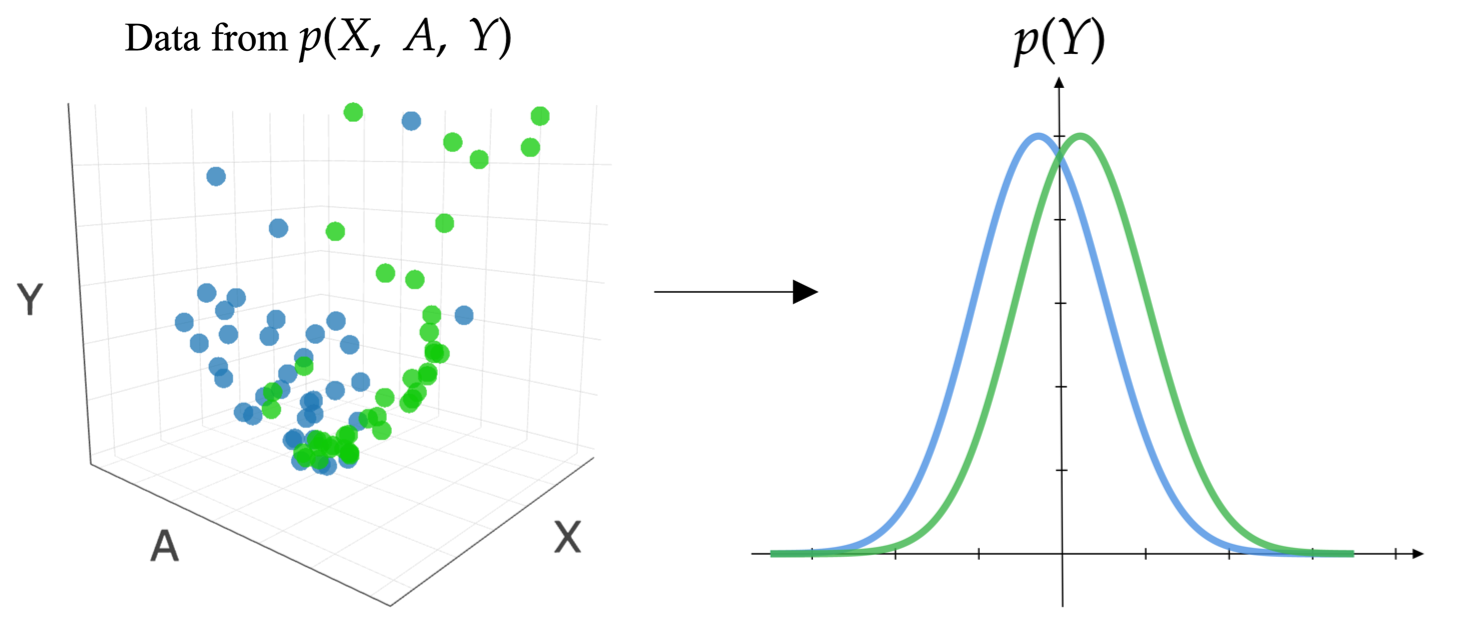
\includegraphics[width=0.5\textwidth]{figures/mr/main_pic.png}
%     \caption{Caption}
%     % \vspace{-1cm}
%     \label{fig:my_label}
% \end{wrapfigure}
In contextual bandits, the objective is to select an action $A$, guided by contextual information $X$, to maximize the resulting outcome $Y$. This paradigm is prevalent in many real-world applications such as healthcare, personalized recommendation systems, or online advertising \citep{li2010contextual, bastani2019online, xu2020contextual}. The objective is to perform actions, such as prescribing medication or recommending items, which lead to desired outcomes like improved patient health or higher click-through rates. Nonetheless, updating the policy presents challenges, as na\"ively implementing a new, untested policy may raise ethical or financial concerns. For instance, prescribing a drug based on a new policy poses risks, as it may result in unexpected side effects. As a result, recent research \citep{swaminathan2015counterfactual, wang2017optimal, farajtabar2018more, su2019continuous, metelli2021subgaussian, liu2019triply, sugiyama2012machine, swaminathan2017off} has concentrated on evaluating the performance of new policies (target policy) using only existing data that was generated using the current policy (behaviour policy). This problem is known as Off-Policy Evaluation (OPE).


Current OPE methods in contextual bandits, such as the Inverse Probability Weighting (IPW) \citep{horvitz1952generalization} and Doubly Robust (DR) \citep{dudik2014doubly} estimators primarily account for the policy shift by re-weighting the data using the ratio of the target and behaviour polices to estimate the target policy value. This can be problematic as it may lead to high variance in the estimators in cases of substantial policy shifts. The issue is further exacerbated in situations with large action or context spaces \citep{saito2022off}, since in these cases the estimation of policy ratios is even more difficult leading to extreme bias and variance.
% The problem is worsened in the policy ratios are even harder to estimate in these cases. 
% even when the distribution of outcome $Y$ changes minimally.
% \jef{Nonetheless, these methods possess a fundamental limitation, as they explicitly account for the shift between behavior and target policies when estimating the expected target policy value.} 
% As a result, the estimators may demonstrate high variance in cases of substantial policy shifts, even when the outcome distribution in $Y$ changes minimally. 
% This high variance in estimators can lead to unreliable and potentially vacuous outputs. 

% In light of these concerns, since our goal is to estimate the expected outcome $Y$ under a new target policy, we show that directly considering the shift in the marginal distribution of outcomes $Y$ rather than the shift in the policies leads to a more efficient estimator.

% Given our goal of estimating the expected outcome $Y$ under a new target policy, we show that directly considering the shift in the marginal distribution of outcomes $Y$

In this work we show that this problem of high variance in OPE can be alleviated by using methods which directly consider the shift in the marginal distribution of the outcome $Y$ resulting from the policy shift, instead of considering the policy shift itself (as in IPW and DR). To this end, we propose a new OPE estimator for contextual bandits called the Marginal Ratio (MR) estimator, which weights the data directly based on the shift in the marginal distribution of outcomes $Y$ and consequently is much more robust to increasing sizes of action and context spaces than existing methods like IPW or DR. 
% Since our goal is to estimate the expected outcome $Y$ under a new target policy, we show that 
% the problem of high variance that arises as a result of weighting the data using policy ratios can be circumvented by instead weighting the data directly based on the shift in the marginal distribution of outcomes $Y$.
% the problem of high variance can be alleviated by weighting the data directly based on the shift in the marginal distribution of outcomes $Y$ resulting from the policy shift rather than the policy ratios (as in IPW or DR).
% directly considering the shift in the marginal distribution of outcomes $Y$ rather than 
% To this end, we propose a new OPE estimator for contextual bandits called the Marginal Ratio (MR) estimator, which directly takes into account the shift in the marginal distribution of the outcome and consequently is much more robust to increasing sizes of action and context spaces than existing methods like IPW or DR. 
Our extensive theoretical analyses show that MR enjoys better variance properties than the existing methods making it highly attractive for a variety of applications in addition to OPE. One such application is the estimation of Average Treatment Effect (ATE) in causal inference, for which we show that MR provides greater sample efficiency than the most commonly used methods.

Our contributions in this paper are as follows:
% and can also be used in domains like causal inference for the estimation of Average Treatment Effect (ATE) where it leads to desirable properties such as increased sample efficiency 
% Additionally, we theoretically show that MR enjoys better variance properties than
% achieves significant variance reduction compared to 
% conventional methods (like IPW or DR) and consequently is much more robust to increasing sizes of action and context spaces.
% Additionally, we also show that the MR estimator can be applied in causal inference for the estimation of Average Treatment Effect (ATE). We demonstrate theoretically and empirically that the MR estimator is more sample efficient than existing methods. Our contributions in this paper are:



% by weighting the samples based on how relevant the observed \emph{outcome} is to the target outcome distribution.

% Our proposed method aims to offer a more robust solution, mitigating the adverse effects of high variance and providing a reliable alternative to existing OPE techniques. 
% At a high level, instead of weighting the samples based on the policy shift as in IPW, the MR estimator weights the samples based on how relevant the observed \emph{outcome} is to target outcome distribution.

% Current OPE methods in contextual bandits, such as the inverse propensity weighting (IPW) \citep{horvitz1952generalization} and doubly robust (DR) \citep{dudik2014doubly} estimators, have gained considerable popularity in practice due to their ability to estimate the expected value of a modified policy. However, these methods have an inherent limitation, as they explicitly consider the shift between behavior and target policies when estimating the target policy value. Consequently, the estimators can exhibit high variance when there is a significant policy shift, even if the change in the outcome distribution is minimal. This issue can be especially pronounced in scenarios with large action or context spaces \citep{saito2022off}.



% Contextual bandits are a prevalent framework \jef{need to rewrite this banditS are A framework doesnt sound right} used in several real-world applications, including healthcare, personalized recommendation systems, and online advertising \citep{li2010contextual, bastani2019online, xu2020contextual}\faaiz{more refs}. In this setup, an agent takes actions $A$ based on contextual information $X$, and receives outcomes $Y$ accordingly. In such settings \jef{Two times start with IN}, evaluating the effectiveness of a new policy without actually deploying it is often desirable \jef{Due to potential financial or ethical reasons + refs}. \jef{Would start this with: Hence, in recent years, researchers have ... }Off-policy evaluation (OPE) is a popular approach that estimates the expected value of a \jef{a or the?} random variable $Y$ under a target policy $\tar$, without deploying the target policy \citep{swaminathan2015counterfactual, wang2017optimal, farajtabar2018more, su2019continuous, metelli2021subgaussian, liu2019triply, sugiyama2012machine, swaminathan2017off}.

% Current OPE methods in contextual bandits focus on the shift in the joint distribution of the context, action, and outcome when estimating the expected value \jef{this sentence is coming out of nowhere}. These methods, such as the inverse propensity weighting (IPW) \citep{horvitz1952generalization} and doubly robust (DR) \citep{dudik2014doubly} estimators, have been highly popular in practice \jef{This should come first}. However, they have a fundamental limitation: they explicitly take the shift between behaviour and target policies into account when estimating target policy value. \jef{we might want to be more vague here in case people do not understand the problem of the ratios, or we have to be way more concrete}


% \jef{I will use AB review from now on :) }


% do not only take the shift in the distribution of the outcome into account, but also the shift in the distribution of the actions. 
% As a result, the estimators can have high variance when the policy shift is large, even if the shift in the outcome distribution is small. This issue can be particularly pronounced in large action or context spaces \citep{saito2022off}.

% To address this limitation, we propose a new OPE estimator for contextual bandits that only takes into account the shift in the marginal distribution of the outcome as a result of the policy shift. Our estimator, called Marginal Ratio (MR) estimator, utilizes the available logged data more efficiently and leads to lower variance than the current state-of-the-art methods. At a high level, instead of weighting the samples based on the policy shift as in IPW, the MR estimator weights the samples based on how relevant the observed \emph{outcome} is to target outcome distribution.
% assigns high weights to the samples where the observed outcomes are most relevant to the target outcome distribution.  

\begin{itemize}
    \item Firstly, we introduce MR, an OPE estimator for contextual bandits, that focuses on the shift in the marginal distribution of $Y$ rather than the joint distribution of $(X, A, Y)$. 
    \flag{We show that MR has favourable theoretical properties compared to existing methods like IPW and DR. Our analysis also encompasses theory on the approximation errors of our estimator. 
    % that MR achieves lower variance than conventional OPE methods like IPW.
    }
    % We provide extensive theoretical comparisons to show  the variance reduction properties of MR compared to existing approaches such as IPW and DR.
    % at MR achieves lower variance than IPW and DR estimators. 
    
    \item Secondly, we explicitly lay out the connection between MR and  Marginalized Inverse Propensity Score (MIPS) \cite{saito2022off}, a recent state-of-the-art contextual bandits OPE method, and prove that MR attains lowest variance among a generalized family of MIPS estimators. 
    \item Thirdly, we show that the MR estimator can be applied in the setting of causal inference to estimate average treatment effects (ATE), and theoretically prove that the resulting estimator is more data-efficient with higher accuracy and lower variance than commonly used methods. 
    \item Finally, we verify all our theoretical analyses through a variety of experiments on synthetic and real-world datasets and empirically demonstrate that the MR estimator achieves better overall performance compared to current state-of-the-art methods. 
\end{itemize}
% Firstly, we introduce MR, an OPE estimator for contextual bandits that focuses on the shift in the marginal distribution of $Y$ rather than the joint distribution of $(X, A, Y)$. Specifically, we provide extensive theoretical comparisons which show that MR achieves lower variance than classical importance-weighted estimators like IPW and DR. Our analysis also encompasses theory on the estimation errors of our estimator. Secondly, we explicitly layout the connection between MR and  Marginalized Inverse Propensity Score (MIPS) \cite{saito2022off}, a recent state-of-the-art contextual bandits OPE method, and demonstrate that MR attains lowest variance among a generalized family of MIPS estimators. Thirdly, we show that the MR estimator can be applied in the setting of causal inference to estimate average treatment effects (ATE), and theoretically prove that the resulting estimator is more data-efficient with higher accuracy and lower variance than commonly used methods. Finally, we verify all our theoretical analyses through a variety of experiments on synthetic and real-world datasets and empirically demonstrate that the MR estimator achieves better overall performance compared to current state-of-the-art methods. 

%  Our contributions in this paper are fourfold.
% \begin{enumerate}[label=\roman*.]
%     \item We introduce MR, an OPE estimator for contextual bandits that focuses on the shift in the marginal distribution of $Y$ rather than the joint distribution of $(X, A, Y)$. Specifically, we provide extensive theoretical comparisons 
%     which show that MR achieves lower variance than classical importance-weighted estimators like IPW and DR.
%     Our analysis also encompasses theory on the estimation errors of our estimator.
%     % In addition, we provide convergence rates for our estimator.
%     % Moreover, we show that MR is likely to achieve lower variance than the DR method when the dimensions of context $X$ are large.
%     % \item We provide theoretical results comparing the performance of MR against the most commonly used OPE estimators for contextual bandits. We prove that the variance of our estimator is lower than that of the classical importance-weighted estimator (IPW). Additionally, we contrast MR against the recently proposed MIPS estimator \citep{saito2022off} and show that MR achieves the optimal variance over the class of all MIPS estimators.
%     \item We explicitly layout the connection between MR and  Marginalized Inverse Propensity Score (MIPS) \cite{saito2022off}, a current state-of-the-art contextual bandits OPE method, and demonstrate that MR attains lowest variance among a generalized family of MIPS estimators.
%     \item We show that the MR estimator can be applied in the setting of causal inference to estimate average treatment effects (ATE), and theoretically prove that the resulting estimator is more data-efficient with higher accuracy and lower variance than commonly used methods.
%     \item We verify all our theoretical analyses through a variety of experiments on synthetic and real-world datasets and empirically demonstrate that the MR estimator achieves better overall performance compared to current state-of-the-art methods.
%     % \item We show that the MR estimator can be applied in the setting of causal inference to estimate average treatment effects (ATE), and leads to a more data-efficient estimator with higher accuracy and lower variance than the most commonly used methods.
%     % \item We verify our analysis on a variety of experiments on synthetic datasets as well as real-world datasets. We empirically show that MR achieves better performance overall compared to the current state-of-the-art methods.
% \end{enumerate}

% First, we propose a new off-policy evaluation (OPE) estimator, called MR, which only takes into account the shift in the marginal distribution of $Y$ instead of the joint distribution of $(X, A, Y)$. Second, we provide theoretical results comparing the performance of MR against the most commonly used OPE estimators for contextual bandits. We prove that the variance of our estimator is lower than that of the classical importance-weighted estimator (IPW). Additionally, we contrast MR against the recently proposed MIPS estimator \citep{saito2022off} and show that MR achieves the optimal variance over the class of all MIPS estimators. Third, we show that the MR estimator can be applied in the setting of causal inference to estimate average treatment effects (ATE), and leads to a more data-efficient estimator with high accuracy and low variance than the most commonly used methods.  Finally, we verify our analysis on a variety of experiments on synthetic datasets as well as real-world datasets. We empirically show that MR achieves better performance overall compared to the current state-of-the-art methods. 
% Our proposed method, MR, can therefore be seen as a significant contribution to the field of off-policy evaluation for contextual bandits.

% Specifically, we provide theoretical results showing that the variance of MR is lower than those of the classical IPW estimator, and the recently proposed MIPS estimator \citep{saito2022off}. We also show that MR achieves the optimal variance over the class of all MIPS estimators.

% In addition to the theoretical analysis, we evaluate the performance of MR on both synthetic and real-world classification datasets. Our experiments demonstrate that MR achieves better performance overall compared to the existing methods. Overall, our proposed MR estimator presents a significant contribution to the OPE problem in contextual bandits, providing a more efficient and accurate way to estimate the expected value of a random variable under a target policy


\section{Background}
\subsection{Setup and Notation} \label{sec:setup_notation}
We consider the standard contextual bandit setting. Let $X\in\Xspace$ be a context vector (e.g., user features), $A\in \Aspace$ denote an action (e.g., recommended website to the user), and $Y\in \Yspace$ denote a scalar reward or outcome (e.g., whether the user clicks on the website). The outcome and context are sampled from unknown probability distributions $p(y\mid x, a)$ and $p(x)$ respectively. Let $\D\coloneqq \{(x_i, a_i, y_i)\}_{i=1}^n$ be a historically logged dataset with $n$ observations, generated by a (possibly unknown) \emph{behaviour policy} $\beh(a\mid x)$.
Specifically, $\D$ consists of i.i.d. samples from the joint density under\textit{ behaviour policy},
\begin{align}
    \pbeh(x, a, y) \coloneqq p(y\mid x, a)\, \textcolor{blue}{\beh(a\mid x)}\,p(x). \label{eq:behav-joint-factorisation}
\end{align}
We denote the joint density of $(X, A, Y)$ under the \textit{target policy} as
\begin{align}
    \ptar(x, a, y) \coloneqq p(y\mid x, a)\, \textcolor{red}{\tar(a\mid x)}\,p(x). \label{eq:tar-joint-factorisation}
\end{align}

Moreover, we use $\pbeh(y)$ to denote the marginal density of $Y$ under the behaviour policy, 
\begin{align*}
    \pbeh(y) &= \int_{\Aspace \times \Xspace} \pbeh(x, a, y)\, \mathrm{d}a \, \mathrm{d}x,
\end{align*}
and likewise for the target policy $\tar$. Similarly, we use $\Ebeh$ and $\Etar$ to denote the expectations under the joint densities $\pbeh(x, a, y)$ and $\ptar(x, a, y)$ respectively.


\myparagraph{Off-policy evaluation (OPE)}
The main objective of OPE is to estimate the expectation of the outcome $Y$ under a given target policy $\tar$, i.e., $\Etar [Y]$, using only the logged data $\D$.
% \[
% \Etar [Y] \coloneqq \E_{(X, A, Y) \sim \ptar}[Y].
% \]


% \paragraph{Notation}
% We use $\pbeh(x, a, y)$ to denote the joint density of $(X, A, Y)$ under the behaviour policy, and $\ptar(x, a, y)$ to denote the joint density under target policy. The joint densities, whose factorisation only differs in the policies, can be written as follows:
% \begin{align}\label{eq:pxay}
%     \pbeh(x, a, y) &= p(y\mid x, a)\, \textcolor{blue}{\beh(a\mid x)}\,p(x), \\
%     \ptar(x, a, y) &= p(y\mid x, a)\, \textcolor{red}{\tar(a\mid x)}\,p(x).
% \end{align}
% The historical logged data $\D$ comprises i.i.d. realisations from the joint density $\pbeh(x, a, y)$.
% Moreover, we use $\pbeh(y)$ to denote the marginal density of $Y$ under the behaviour policy, 
% \begin{align*}
%     \pbeh(y) &= \int_{\Aspace, \Xspace} \pbeh(x, a, y)\, \mathrm{d}a \, \mathrm{d}x,
% \end{align*}
% and likewise for the target policy $\tar$. Similarly, we use $\Ebeh$ and $\Etar$ to denote the expectations under the joint densities $\pbeh(x, a, y)$ and $\ptar(x, a, y)$ respectively.

% \paragraph{Off-policy evaluation}
% Given logged data $\D$, our goal is to estimate the following expectation
% \[
% \Etar [Y] \coloneqq \E_{(X, A, Y) \sim \ptar}[Y].
% \]

Throughout this work, we assume that the support of the target policy $\tar$ is included in the support of the behaviour policy $\beh$. This is to ensure that importance sampling yields unbiased off-policy estimators, and is satisfied for exploratory behaviour policies such as the $\epsilon$-greedy policies. 
\begin{assumption}[Support]
    For any $x \in \Xspace, a \in \Aspace$,  $\tar(a\mid x) >0 \implies \beh(a\mid x) >0$. 
\end{assumption}
% This is a mild assumption which
 

\subsection{Existing off-policy evaluation methodologies}
Next, we will present some of the most commonly used OPE estimators before outlining the limitations of these methodologies. This motivates our proposal of an alternative OPE estimator. 

The value of the target policy can be expressed as the expectation of outcome $Y$ under the target data distribution $\ptar(x, a, y)$.
% The policy value of target policy $\tar$ can be written as:
% \[
% \Etar[Y] = \int_{\Xspace, \Aspace, \Yspace} y\, \ptar(x, a, y) \, \mathrm{d}x \, \mathrm{d}a \, \mathrm{d}y.
% \]
However in most cases, we do not have access to samples from this target distribution and hence we have to resort to importance sampling methods.
\paragraph{Inverse Probability Weighting (IPW) estimator}
One way to compute the target policy value, $\Etar[Y]$, when only given data generated from $\pbeh(x, a, y)$ is to rewrite the policy value as follows:
% _{\Xspace, \Aspace, \Yspace}
\begin{small}
\begin{align*}
    \Etarred[Y] =
    \int y \, \ptar(x, a, y) \,\mathrm{d}y \, \mathrm{d}a\, \mathrm{d}x   =
    \int y \, \underbrace{\frac{\ptar(x, a, y)}{\pbeh(x, a, y)}}_{\rho(a,x)}\, \pbeh(x, a, y) \,\mathrm{d}y \, \mathrm{d}a\, \mathrm{d}x =
    % \Ebehblue\left[Y\,\frac{\ptar(X, A, Y)}{\pbeh(X, A, Y)} \right] = 
    \Ebehblue\left[Y\,\rho(A, X)\right],
\end{align*}
\end{small} 
where 
$
\rho(a, x) \coloneqq \frac{\ptar(x, a, y)}{\pbeh(x, a, y)} = \frac{\tar(a|x)}{\beh(a|x)}
$, given the factorizations in Eqns. \eqref{eq:behav-joint-factorisation} and \eqref{eq:tar-joint-factorisation}.
This leads to the commonly used \emph{Inverse Probability Weighting (IPW)} \citep{horvitz1952generalization} estimator:
\[
\thetaipw \coloneqq \frac{1}{n}\sum_{i=1}^n \rho(a_i, x_i)\,y_i.
\]
When the behaviour policy is known, IPW is an unbiased and consistent estimator. However, it can suffer from high variance, especially as the overlap between the behaviour and target policies decreases. 

\myparagraph{Doubly Robust (DR) estimator} 
To alleviate the high variance of IPW, \cite{dudik2014doubly} proposed a \emph{Doubly Robust (DR)} estimator for OPE. 
DR uses an estimate of the conditional mean $\hat{\mu}(a, x) \approx\E[Y\mid X=x, A=a]$ (\emph{outcome model}), as a control variate to decrease the variance of IPW. It is also doubly robust in that it yields accurate value estimates if either the importance weights $\rho(a, x)$ or the outcome model $\hat{\mu}(a, x)$ is well estimated \citep{dudik2014doubly, jiang2016doubly}. 
The DR estimator for $\Etar[Y]$ can be written as follows:
\[
\thetadr = \frac{1}{n} \sum_{i=1}^n \rho(a_i, x_i)\,(y_i - \hat{\mu}(a_i, x_i)) + \hat{\eta}(\tar),
% \vspace{-0.7mm}
\]
where
$
\hat{\eta}(\tar) = \frac{1}{n} \sum_{i=1}^n \sum_{a'\in \Aspace} \hat{\mu}(a', x_i) \tar(a'\mid x_i) \approx \E_{\tar}[\hat{\mu}(A, X)]$. Here, $\hat{\eta}(\tar)$ is referred to as the Direct Method (DM) as it uses $\hat{\mu}(a, x)$ directly to estimate target policy value. 

\subsection{Limitation of existing methodologies} 
To estimate the value of the target policy $\tar$, the existing methodologies consider the shift in the joint distribution of $(X, A, Y)$  as a result of the policy shift (by weighting samples by policy ratios). As we show in Section \ref{subsec:comparison}, considering the joint shift can lead to inefficient policy evaluation and high variance especially as the policy shift increases \citep{li2018addressing}.
Since our goal is to estimate $\Etar[Y]$, we will show in the next section that considering only the shift in the marginal distribution of the outcomes $Y$ from $\pbeh(Y)$ to $\ptar(Y)$, leads to a more efficient OPE methodology compared to existing approaches.

To better comprehend why only considering the shift in the marginal distribution is advantageous, let us examine an extreme example where we assume that $Y \indep A \mid X$, i.e., the outcome $Y$ for a user $X$ is independent of the action $A$ taken. In this specific instance, $\Etar[Y] = \Ebeh[Y] \approx 1/n\sum_{i=1}^n y_i,$ indicating that an unweighted empirical mean serves as a suitable unbiased estimator of $\Etar[Y]$. However, IPW and DR estimators use policy ratios $\rho(a, x)  = \frac{\tar(a \mid x)}{\beh(a \mid x)}$ as importance weights. In case of large policy shifts, these ratios may vary significantly, leading to high variance in IPW and DR.

In this particular example, the shift in policies is inconsequential as it does not impact the distribution of outcomes $Y$. Hence, IPW and DR estimators introduce additional variance due to the policy ratios when they are not actually required. This limitation is not exclusive to this special case; in general, methodologies like IPW and DR exhibit high variance when there is low overlap between target and behavior policies \citep{li2018addressing} even if the resulting shift in marginals of the outcome $Y$ is not significant.
% This limitation is not exclusive to this special case; in general, methodologies like IPW and DR that use policy ratios as importance weights exhibit high variance when there is low overlap between target and behavior policies \citep{li2018addressing} or when the action and/or context spaces are large \citep{saito2022off}.

Therefore, we propose the \emph{Marginal Ratio (MR)} OPE estimator for contextual bandits in the subsequent section, which circumvents these issues by focusing on the shift in the marginal distribution of the outcomes $Y$. Additionally, we provide extensive theoretical insights on the comparison of MR to existing state-of-the-art methods, such as IPW and DR.

% To estimate the value of the target policy $\tar$, the existing methodologies consider the shift in the joint distribution of $(X, A, Y)$ as a result of the policy shift. As we show in Section \ref{subsec:comparison}, considering the joint shift can lead to inefficient policy evaluation and high variance especially as the policy shift increases \citep{li2018addressing}.
% Since our goal is to estimate $\Etar[Y]$, we will show in the next section that considering only the shift in the marginal distribution of the outcomes $Y$ from $\pbeh(Y)$ to $\ptar(Y)$, leads to a more efficient OPE methodology compared to existing approaches.

% To gain a better intuitive understanding why only considering the shift in the marginal distribution, let us take this extreme example, where we assume that $Y \indep A \mid X$, i.e. the outcome $Y$ of a user $X$ does not depend on the action taken. In this special example, $\Etar[Y] = \Ebeh[Y] \approx 1/n\sum_{i=1}^n y_i,$ and therefore, an unweighted empirical mean should be a good unbiased estimator of $\Etar[Y]$. However, the IPW and DR estimators use the policy ratios as importance weights since $\ptar(x, a, y)/\pbeh(x, a, y) = \tar(a \mid x)/\beh(a \mid x)$, and hence yield a higher variance estimator. 

% In this specific example, the shift in policies is meaningless as it has no effect on the distribution of outcomes $Y$, and therefore, the IPW and DR estimators incur extra variance due to the importance ratios when they are in fact not needed. This limitation is not restricted to this special case and in general, methodologies like IPW and DR which use policy ratios as importance weights will have high variance whenever there is low overlap between target and behaviour policies \citep{li2018addressing} or whenever the action and/or context spaces are large \citep{saito2022off}.

% Hence, we propose \emph{Marginal Ratio (MR)} OPE estimator for contextual bandits in the next section, which avoids these problems by only considering the shift in the marginal distribution of the outcomes $Y$. In addition, using the MR estimator, we are able to gain novel theoretical insights compared to existing SOTA methods such as IPW and DR methods in terms of variance reduction.






% Since our goal is to estimate $\Etar[Y]$, it suffices to consider only the shift in the marginal distribution of the outcomes $Y$ from $\pbeh(y)$ to $\ptar(y)$. Instead, methodologies like IPW and DR consider the shift in the joint distribution of $(X, A, Y)$ which can lead to inefficient policy evaluation and high variance especially as the policy shift increases \citep{li2018addressing}.
% In the next section, we propose \emph{Marginal Ratio (MR)} OPE estimator which circumvents the limitations outlined above, by only considering the shift in the marginal distribution of the outcomes $Y$. 
% Similarly, we could also consider another example, where the action $a \in [-100, 100]$ is related to $Y$ through a simple function such as $Y=x$ for $a < 0$ and $Y=-x$ for $a > 0$. In this case, modelling the ratio of the policy which for ever action, would unnecessarily complicate as computation. \jef{to be completed}
% \jef{TODO} The following special case makes this idea more concrete. Assume that $Y \indep A \mid X$, i.e. the outcome $Y$ of a user $X$ does not depend on the action taken. In this case $\Etar[Y] = \Ebeh[Y] \approx 1/n\sum_{i=1}^n y_i,$ and therefore, an unweighted empirical mean should be a good unbiased estimator of $\Etar[Y]$. However, the IPW and DR estimators use the policy ratios as importance weights since $\ptar(x, a, y)/\pbeh(x, a, y) = \tar(a \mid x)/\beh(a \mid x)$, and hence yield a weighted estimator. \faaiz{to be fixed}

\section{Marginal Ratio (MR) estimator}
 
% \subsection{Marginal Ratio (MR) estimator}
% The main insight of our methodology is to weight the outcomes using the ratio of marginal density of the outcome $Y$, i.e.,
Our method's key insight involves weighting outcomes by the marginal density ratio of outcome $Y$:
\begin{align*}
\Etarred[Y] &= \int_{\Yspace} y \, \ptar(y)\, \mathrm{d}y = \int_\Yspace y\, \frac{\ptar(y)}{\pbeh(y)} \, \pbeh(y) \, \mathrm{d}y = \Ebehblue\left[Y\, w(Y) \right],
\end{align*}
where 
$
w(y) \coloneqq \frac{\ptar(y)}{\pbeh(y)}.
$
This leads to the Marginal Ratio OPE estimator:
\begin{align*}
    \thetamr \coloneqq \frac{1}{n}\sum_{i=1}^n w(y_i) \, y_i.
\end{align*}

In Section \ref{subsec:comparison} we prove that by only considering the shift in the marginal distribution of outcomes, the MR estimator achieves a lower variance than the standard OPE methods. In fact, this estimator does not depend on the shift between target and behaviour policies directly. Instead, it depends on the shift between the marginals $\pbeh(y)$ and $\ptar(y)$.
% Moreover, when the weights $w(y)$ are known exactly, the MR estimator is unbiased and consistent.
% \jef{I recon we can chuck this}
% \jef{Need to change and think as well} Recall that in our previous example with $Y \indep A\mid X$, any policy shift has no effect on the marginal outcome distribution and the weights $w(y)\equiv 1$ for any target and behaviour policies. Therefore $\thetamr = 1/n \sum_{i=1}^n y_i$, i.e., MR leads to an unweighted estimator which is unbiased and does not incur any extra variance arising from the importance weights $\tar(a\mid x)/\beh(a\mid x)$.
% Before we go on to prove the variance reduction, we first outline how to efficiently compute the weights $w(y)$ using the logged data $\D$.
% To start, let us outline an efficient way to estimate the weights $w(y)$ using the logged data $\D$, before moving on to prove the variance reduction.

\myparagraph{Estimation of $w(y)$} When the weights $w(y)$ are known exactly, the MR estimator is unbiased and consistent. However, in practice the weights $w(y)$ are often not known and must be estimated using the logged data $\D$. Here, we outline an efficient way to estimate $w(y)$ by first representing it as a conditional expectation, which can subsequently be expressed as the solution to a regression problem.
% \jef{Add references as mentioned by Arnaud}
% \begin{align}\label{eq:ratioidentity}
%     w(y)=\frac{\ptar(y)}{\pbeh(y)} =\int_{\Xspace, \Aspace} \frac{\ptar(x,a,y)}{\pbeh(x,a,y)}\,\pbeh(a, x|y)\,\mathrm{d}a\, \mathrm{d}x  
%     % &=\int_{\Xspace, \Aspace} \frac{\pi^{\ast}(a|x)}{\beh (a|x)}\,\pbeh(a, x|y)\,\mathrm{d}a \,\mathrm{d}x \nonumber\\
%     &= \Ebeh\Bigg[ \frac{\pi^{\ast}(A|X)}{\beh (A|X)} \Bigg| \,Y=y \Bigg]. 
% \end{align}
% \faaiz{make this a complete sentence}
\begin{lemma}\label{lemma:weights-est}
Let $w(y)=\frac{\ptar(y)}{\pbeh(y)}$ and $\rho(a, x) = \frac{\tar(a\mid x)}{\beh(a\mid x)}$, then $w(y) = \Ebeh\left[ \rho(A, X) \mid \,Y=y \right]$, and,
% \[
% w(y)= \Ebeh\left[ \rho(A, X) \mid \,Y=y \right], \quad \textup{and consequently,} \quad w = \arg\min_{f} \, \Ebeh \left[(\rho(A, X)-f(Y))^2\right]. 
% \]
% Additionally,
\begin{align}
 w = \arg\min_{f} \, \Ebeh \left[(\rho(A, X)-f(Y))^2\right]. \label{eq:weights-obj}
\end{align}
\end{lemma}
% \vspace{-2mm}
Lemma \ref{lemma:weights-est} allows us to approximate $w(y)$ using a parametric family $\{f_\phi: \mathbb{R}\rightarrow \mathbb{R} \mid \phi \in \Phi\}$ (e.g.\ neural networks) and defining $\hat{w}(y)\coloneqq f_{\phi^*}(y)$, where $\phi^*$ solves the regression problem in Eq. \eqref{eq:weights-obj}. 

% Hence, the weights $w(y)$ can be estimated by solving the regression problem in Eq. \eqref{eq:weights-obj}. 
% Similar techniques of estimating ratios of marginal densities have also been used in areas like likelihood-free inference \citep{brehmer2020mining}.
% Similar techniques have also been used in areas like likelihood-free inference \citep{brehmer2020mining} to estimate the ratio of marginal densities.

% \paragraph{Proof of Lemma \ref{prop:weights-est}}
% This follows directly from the identity \eqref{eq:ratioidentity}. 
% We prove it here for the sake of completeness.
% \begin{align}
%     &\Ebeh \Bigg[\frac{\pi^{\ast}(A|X)}{\beh (A|X)}-f(Y)\Bigg]^2 \nonumber \\
%     &= \mathbb{E}_{X,Y \sim P^{\beh}_{X,Y}} \Big[\E_{A \sim P^{\beh}_{A\mid X,Y}} \Big|\Big|\frac{\pi^{\ast}(A|X)}{\beh (A|X)}-f(X,Y)\Big|\Big|^2\Big] \nonumber \\
%     &= \mathbb{E}_{X,Y \sim P^{\beh}_{X,Y}} \Big[\textup{Var}_{A \sim P^{\beh}_{A\mid X,Y}}\Big[ \frac{\pi^{\ast}(A|X)}{\beh (A|X)} \Big] + \left(\E_{A \sim P^{\beh}_{A\mid X,Y}}\Big[ \frac{\pi^{\ast}(A|X)}{\beh (A|X)} \Big] - f(X,Y) \right)^2 \Big].
%      \label{eq:w-reg}
% \end{align}
% Where, \eqref{eq:w-reg} is minimized if $f(x, y) = \E_{A \sim P^{\beh}_{A\mid X=x,Y=y}}\Big[ \frac{\pi^{\ast}(A|x)}{\beh (A|x)} \Big] = w(x,y)$.

% \begin{align}
%     \theta^* \coloneqq \arg \min_{\theta} \Ebeh \Bigg(\frac{\pi^{\ast}(A|X)}{\beh (A|X)}-f_\theta(Y)\Bigg)^2 \label{eq:weights-loss}
% \end{align}

Note that MR can also be estimated alternatively by directly estimating $h(y) \coloneqq w(y)\,y$ 
% (instead of estimating the weights $w(y)$) 
using a similar regression technique as above and computing $\thetamr = 1/n \sum_{i=1}^n h(y_i)$. We include additional details along with empirical comparisons in Appendix \ref{sec:alt-estimation-method}. 
% In the next section, we provide theoretical analysis comparing the MR estimator with the existing methodologies. 

\begin{comment}
\subsubsection{Alternative estimation method}\label{sec:alt-estimation-method}
When estimating the MR estimator, we can alternatively estimate $h(y) \coloneqq y\,w(y)$ using 
\begin{align*}
    h = \arg\min_{f} \, \Ebeh \Bigg(Y\,\frac{\tar(A|X)}{\beh (A|X)}-f(Y)\Bigg)^2.
\end{align*}
Subsequently, the MR estimator can be written as:
\[
\thetamr = \frac{1}{n}\sum_{i=1}^n h(y_i).
\]
\paragraph{Remark}
These methods outline two different methodologies of estimating MR. In general, it is difficult to say which of the two methods will perform better. Intuitively speaking, in cases where the behaviour of the quantity $Y\,\frac{\tar(A|X)}{\beh (A|X)}$ with varying $Y$ is `smoother' than that of $\frac{\tar(A|X)}{\beh (A|X)}$, the alternative method is expected to perform better. Our empirical results in Appendix \ref{app:experiments} shows that the relative performance of the two methods varies for different data generating mechanisms.

% \faaiz{talk about the comparison between the two methods}

\rob{We could alternatively write $\Etar[Y] = \Ebeh[\Ebeh[Y \, \frac{\pi^\ast(A|X)}{\beh(A|X)} \mid Y]]$, regress $h_\theta(y) \approx \Ebeh[Y \, \frac{\pi^\ast(A|X)}{\beh(A|X)} \mid Y = y]$, and approximate $\Etar[Y] \approx \frac{1}{n} \sum_{i=1}^n h_\theta(Y_i)$. Is there a reason not to prefer this approach?}

\arnaud{indeed Rob, actually i conjecture that this should be better - think of a case where the policy ratio is high in regions where the outcome is null - with Rob's approach you won't need to bother approximating the ratio of marginal returns in those regions... i think that then the theoretical result will be less elegant -- in any case, this should be tried and mentioned in the paper}
\end{comment}

\subsection{Theoretical analysis}\label{subsec:comparison}
Recall that the traditional OPE estimators like IPW and DR use importance weights which account for the the shift in the joint distributions of $(X, A, Y)$. In this section, we prove that by considering only the shift in the marginal distribution of $Y$ instead, MR achieves better variance properties than these estimators.
% , which considers the shift in the marginal distribution of $Y$, achieves lower variance than the existing methods. 
Our analysis in this subsection assumes that the ratios $\rho(a, x)$ and $w(y)$ are known exactly. Since the OPE estimators considered are unbiased in this case, 
our analysis of variance is analogous to that of the mean squared error (MSE) here.
% Since the OPE estimators considered are unbiased in this case, we only need to compare the variance of these estimators. 
We address the case where the weights are not known exactly in Section \ref{subsec:weight-estimation-error}.
First, we make precise our intuition that the shift in the joint distribution of $(X, A, Y)$ is `greater' than the shift in the marginal distribution of outcomes $Y$. 
We formalise this using the notion of $f$-divergences.
\begin{proposition}\label{tv_prop}
Let $f:[0, \infty) \rightarrow \mathbb{R}$ be a convex function with $f(1)=0$, and $\textup{D}_f(P || Q)$ denotes the $f$-divergence between distributions $P$ and $Q$. Then,
\[
\textup{D}_f\left(\ptar(x,a,y)\,||\, \pbeh(x,a,y)\right) \geq \textup{D}_f\left(\ptar(y)\,||\, \pbeh(y)\right).
\]
\end{proposition}

\begin{comment}
\begin{proposition}\label{tv_prop}
Let $\textup{TV}(P, Q)$ denote the total variation distance between densities $P$ and $Q$. Then,
$$
\textup{TV}\left(\pbeh(x, a, y), \ptar(x, a, y)\right) \geq \textup{TV}\left(\pbeh(y), \ptar(y)\right).
$$
\end{proposition}
\begin{proof}
\begin{align}
    \textup{TV}\left(\pbeh(x, a, y), \ptar(x, a, y)\right) &= 1/2 \int_{\Xspace, \Aspace,\Yspace} |\pbeh(x, a, y) - \ptar(x, a, y) | \, \mathrm{d}x \,\mathrm{d}a \, \mathrm{d}y \nonumber\\
    &\geq 1/2 \int_\Yspace\left| \int_{\Xspace,\Aspace} \pbeh(x, a, y) - \ptar(x, a, y) \, \mathrm{d}a \, \mathrm{d}x \right| \mathrm{d}y \nonumber\\
    &= 1/2 \int_\Yspace |\pbeh(y) - \ptar(y)|\, \mathrm{d}y \nonumber\\
    &= \textup{TV}\left(\pbeh(y), \ptar(y)\right) \nonumber
\end{align}
\end{proof}
\end{comment}
\paragraph{Intuition}
Proposition \ref{tv_prop} shows that the shift in the joint distributions is at least as `large' as the shift in the marginals of the outcome $Y$. Traditional OPE estimators, therefore take into consideration more of a distribution shift than needed, and consequently lead to inefficient estimators. In contrast, the MR estimator mitigates this problem by only considering the shift in the marginal distributions of outcomes resulting from the policy shift. 
% This intuition is made precise in \faaiz{ref}, which shows that the number of datapoints needed for accurate importance sampling estimates is directly related to the KL-divergence between two distributions
This provides further intuition on why the MR estimator has lower variance compared to existing methods. 
% Moreover, this result can also be used to prove that th
% \flag{This intuition is also supported by \cite{chatterjee2018sample}.}
% , which shows that the accuracy of an importance sampling mean estimate is directly related to the KL-divergence (which is an $f$-divergence) between the data distribution and the target distribution.
% For instance, in our example with $Y \indep A\mid X$, the weights $w(y)\equiv 1$ for any target and behaviour policies as any policy shift has no effect on the marginal outcome distribution, and therefore $\thetamr = 1/n \sum_{i=1}^n y_i$. 

% \jef{possible remove}
% Additionally, we emphasise the generality of Proposition \ref{tv_prop}, as it holds for the large class of $f$-divergences which includes the most commonly used divergences such as KL-divergence, total variation distance and $\chi^2$-divergences. In particular, by using $f(x) = (x-1)^2$ in Proposition \ref{tv_prop} we obtain that the variance of marginal density ratios $w(Y)$ is smaller than that of the policy ratio $\rho(A, X)$. This provides further intuition on why the MR estimator has lower variance compared to existing methods.
% This also results in the MR estimator having a lower variance than the IPW estimator. 

\begin{comment}
    
In fact, as we show next, Proposition \ref{tv_prop} implies that on average the marginal density ratio is closer to 1 than the joint density ratio (i.e., the policy ratio), and moreover, the variance of marginal density ratio is also smaller than that of the policy ratio. 
% using $f(x) = |x - 1|$ it follows straightforwardly from Proposition \ref{tv_prop} that on average the marginal density ratio is closer to 1 than the joint density ratio (i.e., the policy ratio). We formalise this in the following corollary.
\begin{corollary}
\begin{align*}
    f(x) = |x-1| \quad\textup{in Proposition \ref{tv_prop}} &\implies \Ebeh\left|\rho(A, X) - 1 \right| \geq \Ebeh\left|w(Y) - 1 \right|,\\
    f(x) = (x-1)^2 \quad\textup{in Proposition \ref{tv_prop}} &\implies \Vbeh(\rho(A, X)) \geq \Vbeh(w(Y)),
\end{align*}
where $\rho(a, x) \coloneqq \frac{\ptar(x, a, y)}{\pbeh(x, a, y)} =\frac{\tar(a|x)}{\beh(a|x)}$.
% Using $f(x) = |x-1|$ in Proposition \ref{tv_prop}: $\Ebeh\left|\rho(A, X) - 1 \right| \geq \Ebeh\left|w(Y) - 1 \right|$.\\
% Using $f(x) = (x-1)^2$ in Proposition \ref{tv_prop}: $\Vbeh(\rho(A, X)) \geq \Vbeh(w(Y))$.
% % \begin{align}
% %     \Ebeh\left|\rho(A, X) - 1 \right| \geq \Ebeh\left|w(Y) - 1 \right|
% % \end{align}
\end{corollary}
\paragraph{Intuition} As a consequence of only considering the marginal shift, the weights $w(Y)$ are `closer' to 1 on average than the ratio of joint distributions $\rho(A, X)$, and the variance of $w(Y)$ is smaller than that of $\rho(A, X)$. This also results in the MR estimator having a lower variance than the IPW estimator.
% \faaiz{we can also similarly prove that variance of $\rho(A, X)$ is greater than that of $w(Y)$ using $f(x) = (x-1)^2$.}
\end{comment}

\begin{proposition}[Variance comparison with IPW estimator]\label{prop:var_mr}
When the weights $\rho(a, x)$ and $w(y)$ are known exactly, we have that $\Vbeh[\thetamr] \leq \Vbeh[\thetaipw]$. In particular,
\begin{align*}
    \Vbeh[\thetaipw] - \Vbeh[\thetamr]
    = \frac{1}{n} \Ebeh \left[ \Vbeh\left[ \rho(A, X) \mid Y \right]\, Y^2 \right] \geq 0.
\end{align*}
\end{proposition}
\myparagraph{Intuition}
Proposition \ref{prop:var_mr} shows that the variance of MR estimator is smaller than that of the IPW estimator when the weights are known exactly. 
% Since MR is unbiased in this case, our analysis in this section mainly focuses on the variance. We also address the case where the weights are not known exactly in Section \ref{subsec:weight-estimation-error} by analysing the resulting bias and variance of MR. 
Moreover, the proposition also shows that the difference between the two variances will increases as the variance $\Vbeh\left[ \rho(A, X) \mid Y \right]$ increases. This variance is likely to be large when the policy shift between $\beh$ and $\tar$ is large, or when the dimensions of contexts $X$ and/or the actions $A$ is large, and therefore in these cases the MR estimator will perform increasingly better than the IPW estimator.
% The proposition therefore suggests that the MR estimator performs increasingly better than the IPW estimator as the difference between target and behaviour policy increases or the dimension of $\Xspace$ and/or $\Aspace$ increases. 
A similar phenomenon occurs for DR as we show next, even though in this case the variance of MR is not in general smaller than that of DR. 

\begin{proposition}[Variance comparison with DR estimator]\label{prop:var_dr}
When the weights $\rho(a, x)$ and $w(y)$ are known exactly and $\mu(A, X) \coloneqq \E[Y\mid X, A]$, we have that,
\begin{align*}
     \Vbeh[\thetadr] - \Vbeh[\thetamr]
    \geq \frac{1}{n} \Ebeh \left[ \Vbeh\left[\rho(A, X)\,Y \mid Y \right] -  \Vbeh\left[\rho(A, X)\,\mu(A, X) \mid X \right] \right].
\end{align*}
\end{proposition}
\paragraph{Intuition}
Proposition \ref{prop:var_dr} shows that if $\Vbeh\left[ \rho(A, X)\,Y \mid Y \right]$ is greater than $\Vbeh\left[ \rho(A, X)\,\mu(A, X) \mid X \right]$ on average, the variance of the MR estimator will be less than that of the DR estimator. 
% In other words, 
% the MR estimator will achieve lower variance 
% will not always have lower variance than DR, however, 
Intuitively, this will occur when the dimension of context space $\Xspace$ is high because in this case the conditional variance over $X$ and $A$, $\Vbeh\left[\rho(A, X)\,Y \mid Y \right]$ is likely to be greater than the conditional variance over $A$, $\Vbeh\left[ \rho(A, X)\,\mu(A, X) \mid X \right]$. Our empirical results in Appendix \ref{subsec:mips-empirical} are consistent with this intuition.
Additionally, we also provide theoretical comparisons with other extensions of DR, such as Switch-DR \citep{wang2017optimal} and DR with Optimistic Shrinkage (DRos) \citep{su2020doubly} in Appendix \ref{sec:dr-extensions}, and show that a similar intuition applies for these results. 
\flag{We emphasise that the well known results in \cite{wang2017optimal} which show that IPW and DR estimators achieve the optimal \emph{worst case} variance (where the worst case is taken over a class of possible outcome distributions $Y\mid X, A$) are not at odds with our results presented here (as the distribution of $Y\mid X, A$ is fixed in our setting).}
% We can also show that in the special case when $Y \indep (A, X)$, we have that $\Vbeh[\thetadr] \geq \Vbeh[\thetamr]$ \faaiz{show this}. 
% This may not be the case in practice and in Section \faaiz{ref} we consider the case where the weights are not known.

\subsubsection{Comparison with Marginalised Inverse Propensity Score (MIPS) \citep{saito2022off}}\label{subsec:mips-comparison}
In this section, we compare MR against the recently proposed Marginalised Inverse Propensity Score (MIPS) estimator \citep{saito2022off}, which uses a marginalisation technique to reduce variance and provides a robust OPE estimate specifically in contextual bandits with large action spaces. We prove that the MR estimator achieves lower variance than the MIPS estimator and doesn't require new assumptions.
% If the goal is to obtain OPE estimators with low variance, various analogues of the MR estimator can be considered which use marginalisation techniques to reduce the variance of the resulting estimators. The recently proposed Marginalised Inverse Propensity Score (MIPS) estimator \citep{saito2022off} is one such method which uses a marginalisation technique to reduce variance and provide robust OPE estimates specifically in contextual bandits with large action spaces. 


% We prove that the MR estimator achieves a lower variance than the MIPS estimator and unlike the MIPS estimator, does not require introducing any new assumptions. 

\myparagraph{MIPS estimator}
As we mentioned earlier, the variance of the IPW estimator may be high when the action $A$ is high dimensional. To mitigate this, the MIPS estimator assumes the existence of a (potentially lower dimensional) action embedding $E$, which summarises all `relevant' information about the action $A$. Formally, this assumption can be written as follows: 
\begin{assumption}\label{assum:indep-mips}
    The action $A$ has no direct effect on the outcome $Y$, i.e., 
    $$Y \indep A \mid X, E.$$
\end{assumption}
For example, in the setting of a recommendation system where $A$ corresponds to the items recommended, $E$ may correspond to the item categories. Assumption \ref{assum:indep-mips} then intuitively means that item category $E$ encodes all relevant information about the item $A$ which determines the outcome $Y$. Assuming that such action embedding $E$ exists, \cite{saito2022off} prove that the MIPS estimator $\hat{\theta}_{\textup{MIPS}}$, defined as
\[
\hat{\theta}_{\textup{MIPS}} \coloneqq \frac{1}{n}\sum_{i=1}^n \frac{\ptar(e_i, x_i)}{\pbeh(e_i, x_i)}\, y_i = \frac{1}{n}\sum_{i=1}^n \frac{\ptar(e_i\mid x_i)}{\pbeh(e_i \mid x_i)}\, y_i,
\]
provides an unbiased estimator of target policy value $\Etar[Y]$. Moreover,
$\Vbeh[\hat{\theta}_{\textup{MIPS}}] \leq \Vbeh[\thetaipw]$.

\begin{figure}[ht]
% \begin{wrapfigure}{l}{0.4\textwidth}
\centering
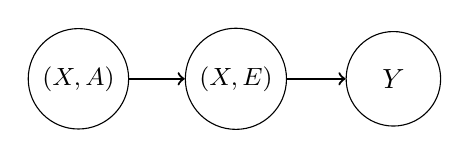
\begin{tikzpicture}

\node[circle,draw, minimum size=1.2cm] (R0) at (0,0) {\begin{small}$(X, A)$\end{small}
};
\node[circle,draw, minimum size=1.2cm] (R1) at (2,0) {\begin{small}$(X, E)$\end{small}};
\node[circle,draw, minimum size=1.2cm] (Y) at (4,0) {$Y$};

\path[->, thick] (R0) edge (R1);
\path[->, thick] (R1) edge (Y);

\end{tikzpicture}
\caption{Bayesian network corresponding to Assumption \ref{assum:indep-mips}.}
\label{fig:embedding_mips}
\vspace{-0.2cm}
% \end{wrapfigure}
\end{figure}


\myparagraph{Intuition}
The context-embedding pair $(X, E)$ can be seen as a representation of the context-action pair $(X, A)$ which contains less `redundant information' regarding the outcome $Y$. Intuitively, the MIPS estimator, which only considers the shift in the distribution of $(X, E)$ is therefore more efficient than the IPW estimator (which considers the shift in the distribution of $(X, A)$ instead). 
% In fact, as the representation $(X, E)$ gets closer to the outcome $Y$ in terms of information content, the variance of the MIPS estimator decreases. We formalise this in Appendix \faaiz{ref}. 

\myparagraph{MR achieves lower variance than MIPS}
Given the intuition above, we should achieve greater variance reduction as the amount of redundant information in the representation $(X, E)$ decreases. We formalise this in Appendix \ref{app:gmips} and show that the variance of MIPS estimator decreases as the representation gets closer to $Y$ in terms of information content. As a result, we achieve the greatest variance reduction by considering the marginal shift in the outcome $Y$ itself (as in MR) rather than the shift in the representation $(X, E)$ (as in MIPS). The following result formalizes this finding. 
% \jef{Ask Arnaud and Rob}
% As such, the greatest variance reduction is achieved when instead of considering the shift in the representation $(X, E)$ as in MIPS, we consider the marginal shift in the outcome $Y$ itself as in the MR estimator. The following results formalises this:
\begin{theorem}\label{prop:mips_main_text}
    When the weights $w(y)$, $\frac{\ptar(e, x)}{\pbeh(e, x)}$ and $\rho(a, x)$ are known exactly, then under Assumption \ref{assum:indep-mips}, 
    \begin{align*}
        \Ebeh[\thetamr] = \Ebeh[\hat{\theta}_{\textup{MIPS}}] = \Etar[Y], \quad \textup{and} \quad \Vbeh[\thetamr] \leq \Vbeh[\hat{\theta}_{\textup{MIPS}}] \leq \Vbeh[\thetaipw].
    \end{align*}
    % \[
    % \Vbeh[\thetamr] \leq \Vbeh[\hat{\theta}_{\textup{MIPS}}] \leq \Vbeh[\thetaipw].
    % \]
\end{theorem}
% \paragraph{Intuition}
This analysis provides a link between the MR and MIPS estimators in the framework of contextual bandits, and shows that the MR estimator achieves lower variance than MIPS estimator while not requiring any additional assumptions (e.g.\ Assumption \ref{assum:indep-mips} as in MIPS). We also verify this empirically in Section \ref{sec:exp-synth} by reproducing the experimental setup in \cite{saito2022off} along with the MR baseline.
% Proposition \ref{prop:mips_main_text} provides us an alternative perspective of the MR estimator. Both, the MIPS and the MR estimators lead to variance reduction by considering a representation of the context-action pair $(X, A)$ which contains less redundant information. However, in the case of the MR estimator, the representation under consideration is the outcome $Y$ itself and therefore it contains precisely the least amount of information necessary to obtain the outcome $Y$. Consequently, the variance of MR estimator is . Additionally, unlike the MIPS estimator, the MR estimator does not require any additional conditional independence assumptions.

% we replace the representation $(X, E)$ by the outcome $Y$ itself. In fact, this recovers the MR estimator.

% In fact, if instead of considering representations of 

% The intuitive reason behind the variance reduction is that the MIPS estimator considers the shift in the joint distribution of $(X, E)$ resulting from the policy shift.

\subsubsection{Weight estimation error}\label{subsec:weight-estimation-error}
% So far our analysis assumes that the behaviour policy $\beh$ and the marginal ratios $w(y)$ are known. However, in practice, both quantities may be unknown and must be estimated from data. To do so, we first split the available logged data $\D$ into training data $\Dtr = \{(x^\tr_i, a^\tr_i, y^\tr_i)\}_{i=1}^m$, which is used for weight estimation, and evaluation data $\Dev = \{(x_i, a_i, y_i)\}_{i=1}^n$, which is used to compute the OPE estimate. 
% % We then estimate the weights $w(y)$ using $\Dtr$ as follows:
% The estimation of weights $w(y)$ involves a two-step process, exclusively utilizing data from $\Dtr$ in each step:
Our analysis so far assumes prior knowledge of the behavior policy $\beh$ and the marginal ratios $w(y)$. However, in practice, both quantities are often unknown and must be estimated from data. To this end, we assume access to an additional training dataset $\Dtr = \{(x^\tr_i, a^\tr_i, y^\tr_i)\}_{i=1}^m$ (for weight estimation), in addition to the evaluation dataset $\D = \{(x_i, a_i, y_i)\}_{i=1}^n$ (for computing the OPE estimate). 
% More generally, these datasets can be obtained by splitting the available logged data.
% we first split the available logged data $\D$ into two subsets: the training data $\Dtr = \{(x^\tr_i, a^\tr_i, y^\tr_i)\}_{i=1}^m$ for weight estimation, and the evaluation data $\Dev = \{(x_i, a_i, y_i)\}_{i=1}^n$ for computing the OPE estimate.
The estimation of $\hat{w}(y)$ involves a two-step process that exclusively utilizes data from $\Dtr$:
% The weights $w(y)$ are then estimated using $\Dtr$ as follows:
% In practice, often the behaviour policy $\beh$ is not known and must be estimated through the logged observational data. 
\begin{enumerate}[label=(\roman*)]
    \item First, we estimate the policy ratio $\hat{\rho}(a, x) \approx \frac{\tar(a | x)}{\beh(a | x)}$. This can be achieved by estimating the behaviour policy $\hatbeh$, and defining $\hat{\rho}(a, x)\coloneqq \frac{\tar(a\mid x)}{\hatbeh(a\mid x)}$. Alternatively, $\hat{\rho}(a, x)$ can also be estimated directly by using density ratio estimation techniques as in \cite{sondhi2020balanced}.
    \item Secondly, we estimate the weights $\hat{w}(y)$ using Eq. \eqref{eq:weights-obj} with $\hat{\rho}$ instead of $\rho$.
\end{enumerate}

    % First, we estimate the behaviour policy $\hatbeh$, and define the policy ratio 
    % $
    % \hat{\rho}(A, X)\coloneqq \frac{\tar(a\mid x)}{\hatbeh(a\mid x)}.$
    % and use it to define the estimated ratios $\hat{\rho}(a, x)\coloneqq \tar(a\mid x)/\hatbeh(a\mid x)$.
 
% In this case, the policy ratio $\rho(a, x)$ is not known, and we resort to the use of estimated ratios $\hat{\rho}(a, x)\coloneqq \tar(a\mid x)/\hatbeh(a\mid x)$ instead.
% % This means the policy ratio $\rho(a, x)$ is not known, and must be estimated using the estimated behaviour policy, i.e.\ $\hat{\rho}(a, x)\coloneqq \tar(a\mid x)/\hatbeh(a\mid x)$. 
% The use of this ratio estimate $\hat{\rho}(a, x)$ may introduce bias in the IPW estimator. This also means that we have to rely on the estimated policy $\hatbeh$ to estimate the marginal ratio $w(y)$, which may also introduce a bias in the MR estimator. 

In practice, one may consider splitting $\Dtr$ for each estimation step outlined above. Moreover,
each approximation step may introduce bias and therefore, the MR estimator may have two sources of bias.
% the MR estimator may have two sources of bias: estimation of the behaviour policy $\hatbeh$, and the estimation of weights $\hat{w}(y)$.
% $$
% \hat{w}(y) \approx \Ebeh[\hat{\rho}(A, X)\mid Y=y] \qquad \textup{where, } \qquad  \hat{\rho}(a, x) \coloneqq \frac{\tar(a\mid x)}{\hatbeh(a\mid x)}.
% $$
While classical OPE methods like IPW and DR also suffer from bias because of $\hat{\rho}$ estimation, the estimation of $\hat{w}(y)$ is specific to MR. However, we show below
that given any policy ratio estimate $\hat{\rho}$, if $\hat{w}(y)$ approximates $\Ebeh[\hat{\rho}(A, X)\mid Y=y]$ `well enough' (i.e., the estimation step (ii) shown above is `accurate enough'), 
then MR achieves a lower variance than IPW and incurs little extra bias.

\begin{proposition}\label{prop:bias-and-var-main}
Suppose that the IPW and MR estimators are defined as,
\[
\approxipw \coloneqq \frac{1}{n}\sum_{i=1}^n\hat{\rho}(a_i, x_i)\, y_i, \quad \textup{and }\quad \approxmr \coloneqq \frac{1}{n}\sum_{i=1}^n\hat{w}(y_i)\, y_i,
\]
and define the approximation error as $\epsilon \coloneqq \hat{w}(Y) - \tilde{w}(Y)$, where $\tilde{w}(Y) \coloneqq \Ebeh[\hat{\rho}(A, X)\mid Y]$. Then we have that, $\textup{Bias}(\approxmr) - \textup{Bias}(\approxipw) = \Ebeh[\epsilon\,Y]$. Moreover,
% $\Ebeh[\epsilon] = 0$ and 
% $\epsilon \indep Y$. Then, 
% \begin{align*}
%     \textup{Bias}(\thetamr) &= \textup{Bias}(\thetaipw) \quad \textup{and,} \\
%     n (\Vbeh[\thetaipw] - \Vbeh[\thetamr]) 
%     &= \E_{Y\sim \pbeh(Y)} \left[ \Vbeh\left[ \hat{\rho}(A, X) \mid Y \right]\, Y^2 \right] - \Vbeh[\epsilon]\,\Ebeh[Y^2].
% \end{align*}
\begin{small}
\begin{align}
    \Vbeh[\approxipw] - \Vbeh[\approxmr]
    % &= \frac{1}{n}\left(\underbrace{\Ebeh[\Vbeh[\hat{\rho}(A, X)\,Y\mid Y]]}_{\geq 0} - \Vbeh[\epsilon\,Y] - 2\,\textup{Cov}(\tilde{w}(Y)\,Y, \epsilon\,Y)\right). \label{eq:var-difference-approximate-weights}
    &= \frac{1}{n}(\underbrace{\Ebeh[\Vbeh[\hat{\rho}(A, X)\,Y\mid Y]]}_{\geq 0} - \Vbeh[\epsilon\,Y] - 2\,\textup{Cov}(\tilde{w}(Y)\,Y, \epsilon\,Y)). \label{eq:var-difference-approximate-weights}
\end{align}
\end{small}
% and,
% \begin{align*}
%     &n (\Vbeh[\approxipw] - \Vbeh[\approxmr]) \\
%     &\quad= \Ebeh[\Vbeh[\hat{\rho}(A, X)\mid Y]\,Y^2] - \Vbeh[\epsilon\,Y] - 2\,\textup{Cov}(\Ebeh[\hat{\rho}(A, X)\mid Y]\,Y, \epsilon\,Y).
% \end{align*}
\end{proposition}
% if $\Ebeh[\hat{\rho}(A, X)\mid Y]$ is estimated `well enough', MR achieves a lower variance than IPW and does not incur any extra bias compared to IPW.
\myparagraph{Intuition} The $\epsilon$ term defined in Proposition \ref{prop:bias-and-var-main} denotes the error of the second approximation step outlined above. 
As a direct consequence of this result, we show in Appendix \ref{sec:wide_nns_weight_estimation} that as the error $\epsilon$ becomes small (specifically as $\Ebeh[\epsilon^2]\rightarrow 0$), the difference between biases of MR and IPW estimator becomes negligible.
% The result shows that as the error $\epsilon$ becomes small, i.e. $\epsilon \overset{\textup{a.s.}}{\rightarrow}0$, the difference between biases of MR and IPW estimator decreases. 
Likewise, the terms $\Vbeh[\epsilon\,Y]$ and $\textup{Cov}(\tilde{w}(Y)\,Y, \epsilon\,Y)$ in Eq. \eqref{eq:var-difference-approximate-weights} will also be small and as a result the variance of MR will be lower than that of IPW (as the first term is positive). 

In fact, using recent results regarding the generalisation error of neural networks \citep{lai2023generalization}, we show that when using 2-layer wide neural networks to approximate the weights $\hat{w}(y)$, the estimation error $\epsilon$ declines with increasing training data size $m$. Specifically, under certain regularity assumptions we obtain $\Ebeh[\epsilon^2] = O(m^{-2/3})$. Using this we show that as the training data size $m$ increases, the biases of MR and IPW estimators become roughly equal with a high probability, and
\[
\Vbeh[\approxipw] - \Vbeh[\approxmr] = \frac{1}{n}\,\Ebeh[\Vbeh[\hat{\rho}(A, X)\,Y\mid Y]] + O(m^{-1/3}).
\]
Therefore the variance of MR estimator falls below that of IPW for large enough $m$. The empirical results shown in Appendix \ref{subsec:mips-empirical} are consistent with this result. Due to space constraints, the main technical result has been included in Appendix \ref{sec:wide_nns_weight_estimation}.

% number of training samples $m$ increases, the biases of MR and IPW estimators become roughly equal, whereas the variance of MR estimator falls below that of the IPW estimator. The empirical results shown in Appendix \ref{subsec:additional-experiments} are consistent with this result.
% Moreover, in Theorem \ref{prop:informal}, the estimated policy ratio $\hat{\rho}(a, x)$ is fixed for increasing $m$, i.e., we do not update $\hat{\rho}(a, x)$ as more training data becomes available. While this may seem as a disadvantage for the IPW estimator, we point out that the result also holds when the policy ratio is exact (i.e., $\hat{\rho}(a, x) = \rho(a, x)$) and hence the IPW estimator is unbiased.

% In fact, using recent results regarding the generalisation error of wide neural networks \citep{lai2023generalization}, we can show that when using 2-layer wide neural networks to approximate the weights $\hat{w}(y)$, the estimation error of the second approximation step above scales as $O(m^{-1/3})$ where $m$ is the number of training data used to approximate $\hat{w}(y)$.
% % Using recent results regarding the generalisation error of wide neural networks \citep{lai2023generalization}, we show that when using 2-layer wide neural networks to approximate the weights $\hat{w}(y)$, then under mild assumptions, $\Ebeh[\epsilon^2]\leq O(m^{-2/3})$. Here $m$ is the number of training data used to approximate $\hat{w}(y)$. 
% Due to space constraints, we include an informal statement of the result here. The main technical result has been included in Appendix \ref{sec:wide_nns_weight_estimation}.

% \begin{theorem}[Informal Statement]\label{prop:informal}
% % Let $\mathcal{D}_{tr}$ be training data with $m$ samples $\{(x^\tr_i, a^\tr_i, y^\tr_i)\}_{i=1}^m$.
% Suppose that the IPW and MR estimators are defined as,
% \[
% \approxipw \coloneqq \frac{1}{n}\sum_{i=1}^n\hat{\rho}(a_i, x_i)\, y_i, \quad \textup{and }\quad \approxmr \coloneqq \frac{1}{n}\sum_{i=1}^n\hat{w}(y_i)\, y_i,
% \]
% % and let
% % \[
% % \thetamr = \frac{1}{n}\sum_{i=1}^n\hat{w}(y_i)\, y_i,
% % \]
% where $\hat{w}(y)$ is approximated by minimising the following empirical loss on a training dataset of size $m$, $\mathcal{D}_{tr}\coloneqq \{(x^\tr_i, a^\tr_i, y^\tr_i)\}_{i=1}^m$ (disjoint from evaluation dataset $\{(x_i, a_i, y_i)\}_{i=1}^n$):
% % \[
% %     \mathcal{L}(\theta) = \E_{\mathcal{D}_{tr}}(\hat{\rho}(A, X) - f_\phi(Y))^2.
% % \]
% \[
%     \mathcal{L}(\phi) = \E_{(X, A, Y)\sim \mathcal{D}_{tr}} \left[\left(\hat{\rho}(A, X) - f_{\phi}(Y)\right)^2\right].
% \]
% If $f_\phi$ is a two-layer neural network with large enough width and for sufficiently large $m$, then under the regularity assumptions provided in Appendix \ref{sec:wide_nns_weight_estimation}, the following holds with high probability,
% \begin{align*}
%     |\textup{Bias}(\approxmr) - \textup{Bias}(\approxipw)| &= O(m^{-1/3}),\\
%     \Vbeh[\approxipw] - \Vbeh[\approxmr] &= \frac{1}{n}\underbrace{\Ebeh[\Vbeh[\hat{\rho}(A, X)\mid Y]\, Y^2]}_{\geq 0} + O(m^{-2/3}).
% \end{align*}
% % holds with high probability. 
% \end{theorem}

% \myparagraph{Intuition} This theorem shows that as the number of training samples $m$ increases, the biases of MR and IPW estimators become roughly equal, whereas the variance of MR estimator falls below that of the IPW estimator. The empirical results shown in Appendix \ref{subsec:additional-experiments} are consistent with this result.
% Moreover, in Theorem \ref{prop:informal}, the estimated policy ratio $\hat{\rho}(a, x)$ is fixed for increasing $m$, i.e., we do not update $\hat{\rho}(a, x)$ as more training data becomes available. While this may seem as a disadvantage for the IPW estimator, we point out that the result also holds when the policy ratio is exact (i.e., $\hat{\rho}(a, x) = \rho(a, x)$) and hence the IPW estimator is unbiased.
 
% In this section, we show that under certain assumptions, the use of the estimated importance weights $\hat{w}(y)$ rather than $\hat{\rho}(a, x)$ does not worsen the bias of the resulting OPE estimator. Moreover, if $\hat{w}(y)$ are estimated `well enough', the variance of MR estimator will be lower than that of IPW estimator in this case as well. The following result formalises this:
% \begin{align}
%     \hat{w} = \arg\min_{f} \, \Ebeh \Bigg[\frac{\tar(A|X)}{\hatbeh (A|X)}-f(Y)\Bigg]^2, \label{eq:estimated-marginal-ratio}
% \end{align}
% then the bias in the MR estimator will be equal to the bias in the IPW estimator. This means that in the case when $\beh$ is approximated and the marginal ratio estimate $\hat{w}(y)$ are obtained by exactly regressing to the approximate policy ratios $\hat{\rho}(a, x)$, the biases of the MR and IPW estimators will be identical. Additionally, the result in Proposition \ref{prop:var_mr} straightforwardly extends to this case, showing that if the marginal ratios $\hat{w}(y)$ are estimated `well enough', the variance of MR estimator will be lower than that of IPW estimator in this case as well.

\subsection{Application to causal inference}\label{subsec:application-to-causal-inference}
 Beyond contextual bandits, the variance reduction properties of the MR estimator make it highly useful in a wide variety of other applications. Here, we show one such application in the field of causal inference, where MR can be used for the estimation of average treatment effect (ATE) \citep{pearl2009causality} and leads to some desirable properties in comparison to the conventional ATE estimation approaches. Specifically, we illustrate that the MR estimator for ATE utilizes the evaluation data $\D$ more efficiently and achieves lower variance than state-of-the-art ATE estimators and consequently provides more accurate ATE estimates.
% leads to a significantly more data efficient methodology with  
% This comparative advantage of MR becomes even more apparent when the observational data size is small.
% We show, both theoretically and empirically, that our methodology provides more reliable ATE estimation overall, and performs especially better than other baselines when the number of data is low.
% The MR estimator can also be applied in the setting of causal inference for estimation of average treatment effect (ATE) and leads to more data efficient methodology than many state-of-the-art ATE estimators.
To be concrete, the goal in this setting is to estimate ATE, defined as follows:
% Off-Policy evaluation is widely applied sin causal inference, where often the goal is to estimate the average treatment effect (ATE), defined as follows:
\[
\ate \coloneqq \E[Y(1)-Y(0)].
\]
Here $Y(a)$ corresponds to the outcome under a deterministic policy $\pi_a(a'\mid x) \coloneqq \ind(a'=a)$. Hence any OPE estimator can be used to estimate $\E[Y(a)]$ (and therefore ATE) by considering target policy $\tar = \pi_a$.
% Given an OPE estimator, $\E[Y(a)]$ 
% We can use any OPE estimator with deterministic target policies to estimate the ATE. 
% We provide explicit expressions of ATE estimators using MR, IPW and DR in Appendix \ref{app:causal-inference}.
An important distinction between MR and existing approaches (like IPW or DR) is that, when estimating $\E[Y(a)]$, the existing approaches only use datapoints in $\D$ with $A=a$. To see why this is the case, we note that the policy ratios $\frac{\tar(A|X)}{\beh(A|X)} = \frac{\ind(A=a)}{\beh(A|X)}$ are zero when $A\neq a$. In contrast, the MR weights $\frac{\ptar(Y)}{\pbeh(Y)}$ are not necessarily zero for datapoints with $A\neq a$, and therefore the MR estimator uses all evaluation datapoints when estimating $\E[Y(a)]$. 

As such we show that MR applied to ATE estimation leads to a smaller variance than the existing approaches. Moreover, because MR is able to use all datapoints when estimating $\E[Y(a)]$, MR will generally be more accurate than the existing methods especially in the setting where the data is imbalanced, i.e., the number of datapoints with $A=a$ is small for a specific action $a$.
In Appendix \ref{app:causal-inference}, we formalise this variance reduction of the MR ATE estimator compared to IPW and DR estimators, by deriving analogous results to Propositions \ref{prop:var_mr} and \ref{prop:var_dr}. In addition, we also show empirically in Section \ref{subsec:causal-experiments} that the MR ATE estimator outperforms the most commonly used ATE estimators.
\begin{comment}

\begin{proposition}\label{prop:bias-and-var}
Let 
\[
\thetaipw = \frac{1}{n}\hat{\rho}(a_i, x_i)\, y_i,
\]
where $\hat{\rho}(a, x)\coloneqq \tar(a\mid x)/\hatbeh(a\mid x)$. Additionally, let
\[
\thetamr = \frac{1}{n}\hat{w}(y_i)\, y_i,
\]
where $\hat{w}(y)$ satisfies Eq. $\eqref{eq:estimated-marginal-ratio}$. Then, 
\begin{align*}
    \textup{Bias}(\thetamr) &= \textup{Bias}(\thetaipw) \qquad \textup{and,} \\
    n (\Vbeh[\thetaipw] - \Vbeh[\thetamr]) 
    &= \E_{Y\sim \pbeh(Y)} \left[ \Vbeh\left[ \hat{\rho}(A, X) \mid Y \right]\, Y^2 \right].
\end{align*}
\end{proposition}
More generally, if $\hat{w}$ is a `noisy' estimate of the conditional expectation $\Ebeh[\hat{\rho}(A, X)\mid Y]$, we can obtain similar results regarding the bias and variance of the MR estimators under certain assumptions. 
\end{comment}


% Using recent results regarding the generalisation error of wide neural networks \citep{lai2023generalization}, we show that when using 2-layer wide neural networks to approximate the weights $\hat{w}(y)$, then under mild assumptions, $\Ebeh[\epsilon^2]\leq O(m^{-2/3})$. Here $m$ is the number of training data used to approximate $\hat{w}(y)$. Due to space constraints, we include an informal statement of the result here. The main technical result has been included in Appendix \ref{sec:wide_nns_weight_estimation}.

% Additionally, replacing the true behaviour policy $\beh$ by the estimate $\hatbeh$ in Eq. \eqref{eq:weights-obj} will 

% if we approximate the marginal ratio $w(y)$ using the approximate 



\begin{comment}
    

Specifically, the traditional IPW estimator applied to ATE estimation yields:
\[
\ateipw = \frac{1}{n} \sum_{i=1}^n \rho_{\ate}(a_i, x_i) \times y_i, \qquad \textup{where, } \qquad \rho_{\ate}(a, x) \coloneqq \frac{\mathbbm{1}(a=1) - \mathbbm{1}(a=0)}{\beh (a|x)}.
\]

Simlarly, the MR estimator can be written as
$$
\atemr = \frac{1}{n}\sum_{i=1}^n w_{\ate}(y_i)\times y_i, \qquad \textup{where, } \qquad w_{\ate}(y) = \frac{p_{\pi^{(1)}}(y) - p_{\pi^{(0)}}(y)}{\pbeh(y)},
$$ 
and $\pi^{(a)}(a'\mid x) \coloneqq \mathbbm{1}(a'=a)$ for $a\in \{0,1\}$, and $w_{\ate}(y)$ can be estimated using regression similar to Eq. \eqref{eq:weights-obj}.
\end{comment}
% Again, using the fact that $w_{\ate}(Y) \eqas \E[\rho_{\ate}(A, X)\mid Y]$, we can obtain $w_{\ate}$ by minimising a simple mean-squared loss:
% \begin{align*}
%     w_{\ate} =\arg \min_{f} \Ebeh \Big[\frac{\mathbbm{1}(A=1)- \mathbbm{1}(A=0)}{\beh (A|X)}-f(Y)\Big]^2
% \end{align*}

% For the MR estimator, we don't need to estimate weights for $Y(1)$ and $Y(0)$ separately, as we can combine the two as follows:
% \begin{align}
%     w_{\ate} =\arg \min_{f} \Ebeh \Big[\frac{\mathbbm{1}(A=1)- \mathbbm{1}(A=0)}{\beh (A|X)}-f(Y)\Big]^2 \label{eq:ate-weights-loss}
% \end{align}
% It follows straightforwardly from Lemma \ref{prop:weights-est}, that the function that minimises  \eqref{eq:ate-weights-loss} is equal to 
% \[
% w_{\ate}(y) = \frac{p_{\pi^{(1)}}(y) - p_{\pi^{(0)}}(y)}{\pbeh(y)},
% \] 
% where $\pi^{(a)}(a'\mid x) \coloneqq \mathbbm{1}(a'=a)$ for $a\in \{0,1\}$.
% Then, the MR estimator can be written as
% $$\atemr = \frac{1}{n}\sum_{i=1}^n w_{\ate}(y_i)\times y_i.$$ 
% In contrast, the traditional IPW estimator is of the form:
% \[
% \ateipw = \frac{1}{n} \sum_{i=1}^n \rho_{\ate}(a_i, x_i) \times y_i,
% \]
% where 
% \[
% \rho_{\ate}(a, x) \coloneqq \frac{\mathbbm{1}(a=1) - \mathbbm{1}(a=0)}{\beh (a|x)}.
% \]

\section{Related Work}
Off-Policy evaluation is a central problem both in contextual bandits \citep{dudik2014doubly, wang2017optimal, liu2018breaking, farajtabar2018more, su2019continuous, su2020doubly, kallus2021optimal, metelli2021subgaussian, saito2020open} and in RL \citep{thomas2016data, xie2019advances, kallus2020off, liu2020understanding}. 
Existing OPE methodologies can be broadly categorised into Direct Method (DM), Inverse Probability Weighting (IPW), and Doubly Robust (DR). 
While DM typically has a low variance, it suffers from high bias when the reward model is misspecified \citep{voloshin2021empirical}. 
On the other hand, IPW \citep{horvitz1952generalization} and DR \citep{dudik2014doubly, wang2017optimal, su2020doubly} use policy ratios as importance weights when estimating policy value and suffer from high variance as overlap between behaviour and target policies increases or as the action/context space gets larger \citep{sachdeva2020off, saito2022off}. To circumvent this problem, techniques like weight clipping or normalisation \citep{swaminathan2015counterfactual, swaminathan2015the, chaudhuri2019london} are often employed, however, these can often increase bias.

% The IPW estimator \citep{horvitz1952generalization} can have low bias but suffers from high variance as overlap between behaviour and target policies increases or as the action/context space gets larger \citep{sachdeva2020off, saito2022off}. To circumvent this problem, techniques like weight clipping or normalisation \citep{swaminathan2015counterfactual, swaminathan2015the} are often employed, however, these can often lead to the worsening of bias.



% The second class of methodologies, called the Inverse Probability Weighting (IPW) \citep{horvitz1952generalization}, uses importance weights to estimate the value of the target policy. If the behaviour policy is well-estimated, the IPW estimator will have a low bias. However, IPW can suffer from a high variance especially as the overlap between behaviour and target policies increases, or as the size of action and/or context space increases \citep{sachdeva2020off}. To circumvent this problem, techniques like weight clipping or normalisation \citep{swaminathan2015counterfactual, swaminathan2015the} are often employed, however, these can often lead to the worsening of bias. 

% The DR method \citep{dudik2014doubly} and its extensions \citep{wang2017optimal, su2020doubly} combine the direct method with importance sampling and achieves better overall bias and variance than the IPW method. However, like the IPW method these DR methods also take the shift of joint distributions of $(X, A, Y)$ into consideration when estimating policy value. As we show in Section \ref{subsec:comparison}, this can lead to high variance especially as the policy shift increases or the action and/or context space gets larger. 

In contrast to these approaches, \cite{saito2022off} propose MIPS, which considers the marginal shift in the distribution of a lower dimensional embedding of the action space. While this approach reduces the variance associated with IPW, we show in Section \ref{subsec:mips-comparison} that the MR estimator achieves a lower variance than MIPS while not requiring any additional assumptions (like Assumption \ref{assum:indep-mips}).
% it requires conditional independence assumptions on the embedding $R$, the violation of which may lead to high bias. 
% We show in Section \ref{subsec:mips-comparison} that in comparison, the MR estimator does not require any such conditional independence assumptions, and achieves a lower variance than the MIPS estimator by only considering the shift in the marginal distribution of the reward $Y$. 

In the context of Reinforcement Learning (RL), various marginalisation techniques of importance weights have been used to propose OPE methodologies.
% OPE methodologies using marginalised importance weighting have been proposed 
% \citep{liu2018breaking, xie2019advances, Fujimoto2021deep, rowland2020conditional}
% \citep{thomas2016data, xie2019advances, kallus2020off, liu2020understanding}. 
\cite{liu2018breaking, xie2019advances, kallus2020off} use methods which considers the shift in the marginal distribution of the states, and applies importance weighting with respect to this marginal shift rather than the trajectory distribution. Similarly, \cite{Fujimoto2021deep} use marginalisation for OPE in deep RL, where the goal is to consider the shift in marginal distributions of state and action. Although marginalization is a key trick of these estimators, these techniques do not consider the marginal shift in reward as in MR and are aimed at resolving the curse of horizon, a problem specific to RL. Apart from this, \cite{rowland2020conditional} propose a general framework of OPE based on conditional expectations of importance ratios for variance reduction. While their proposed framework includes reward conditioned importance ratios, this is not the main focus and there is little theoretical and empirical comparison of their proposed methodology with existing state-of-the-art methods like DR. 

Finally we note that the idea of approximating the ratio of intractable marginal densities via leveraging the fact that this ratio can be reformulated as the conditional expectation of a ratio of tractable densities is a standard idea in computational statistics \cite{meng1996simulating} and has been exploited more recently to perform likelihood-free inference \cite{brehmer2020mining}. In particular, while  \cite{meng1996simulating} typically approximates this expectation through Markov chain Monte Carlo, \cite{brehmer2020mining} uses regression instead, however without any theory.
% of this approach has been carried out in \cite{brehmer2020mining}.

% Our work introduces the marginal ratio estimator for OPE in contextual bandits. We provide extensive theoretical and empirical comparisons of our proposed estimator with existing methods, and show that the MR estimator performs especially better than the other methods in large actions and/or context spaces. 
% \faaiz{@Arnaud and Rob: what are your thoughts about this characterisation of \cite{rowland2020conditional}?}

% Our work proposes an OPE methodology for contextual bandits which only considers the shift in the marginal distribution of rewards. In addition, we include extensive theoretical and empirical comparisons of our proposed estimator with existing methods, and show that the MR estimator performs especially better than the other methods in large actions and/or context spaces. 

\begin{comment}
\begin{itemize}
    \item IPW
    \item Double robust methods
    \item Debiased methods 
    \item See related works in \cite{saito2022off}
\end{itemize}
\subsection{Baselines in Contextual Bandits setting}
\begin{itemize}
    \item \cite{thomas2016data, saito2021evaluating, saito2022off,wang2017optimal}
    \item Using ideas from \cite{saito2022off},  we can show that our methodology requires common support of $\pbeh(Y\mid X)$ and $\ptar(Y\mid X)$ which is weaker than requiring common supports of $\beh(A\mid X)$ and $\tar(A\mid X)$, which is needed for IPW estimator. We can show that our estimator has a smaller variance than the methodology proposed by \cite{saito2022off}. Moreover, we should show empirically that, as a consequence of this, our estimator is more robust to heavy-tailed policy ratios. The baselines considered in this paper are the ones to compare against.
    \item \cite{wang2017optimal} proposes a SWITCH estimator for policy evaluation, and show that this estimator is minimax optimal when the hyperparameter $\tau$ is chosen appropriately. Moreover, this estimator is more robust to large (or heavy-tailed) importance weights. It also includes an expression for the variance of the DR estimator which could be useful.
    \item \cite{saito2021evaluating}: In this work, the authors develop Interpretable Evaluation for Offline Evaluation (IEOE), an experimental procedure to evaluate OPE estimators’ robustness to changes in hyperparameters and/or evaluation policies in an interpretable manner. This is more of a review paper.
    \item \cite{liu2019triply}: Could be an interesting baseline. The background section of this paper seems interesting. 
\end{itemize}
\subsection{Marginalised Importance Sampling in Reinforcement Learning}
The main difference between this line of work and our idea is that these works consider the marginal distribution over the states. Instead, we propose considering the marginal distribution over rewards directly. 
\begin{itemize}
    \item \cite{liu2018breaking}: The paper originally proposed avoiding the long horizon problem by computing MIS over state distributions rather than entire trajectories. The marginal ratio in these works is different to ours.  
    \item \cite{Fujimoto2021deep}: Applies the MIS idea to deep RL setting: Marginalized importance sampling (MIS), which measures the density ratio between the state-action occupancy of a target policy and that of a sampling distribution, is a promising approach for off-policy evaluation. However, current state-of-the-art MIS methods rely on complex optimization tricks and succeed mostly on simple toy problems. This paper bridges the gap between MIS and deep reinforcement learning by observing that the density ratio can be computed from the successor representation of the target policy. 
    \item \cite{kallus2020off}: The related works section of this paper is very useful. In this work, the authors propose the use of a marginal importance sampling estimator which is somewhat similar to ours (although not the same). Would be useful to read this in depth.
    \item \cite{xie2019advances}: Avoiding the long horizon problem by computing IS over state distributions rather than trajectories - was already introduced in \cite{liu2018breaking}, which the authors cite sufficiently often in the text. However, the approach the authors take to leveraging this idea is original. The estimation technique for the ratios is also different -- the authors propose a recursive estimation technique to estimate the marginal distribution ratios over states. 
    \item \cite{liu2020understanding} also references MIS estimators. 
    \item \cite{rowland2020conditional}: This paper proposes conditional importance sampling for variance reduction in RL setting. The paper considers a general conditioning strategy, based on conditioning importance weights on different statistics. They also mention reward conditional importance sampling. \textbf{Important paper.} 
\end{itemize}
\end{comment}


\section{Empirical Evaluation}
In this section, we provide empirical evidence to support our theoretical results by investigating the performance of our MR estimator against the current state-of-the-art OPE methods. The code to reproduce our experiments has been made available at: \href{https://github.com/faaizT/MR-OPE}{\textcolor{blue}{github.com/faaizT/MR-OPE}}.
% Here, we present a synthetic data experiment and also consider an application of MR to causal inference. 
% Additional experiments that support our proposed method MR on real-world classification datasets are provided in Appendix \ref{app:experiments} due to space constraints. \faaiz{Squeeze in classification exps in main}
% We first consider a synthetic setup to conduct extensive ablation study
% We evaluate MR estimator on synthetic data to identify the cases where it offers more accurate off-policy evaluation. These experiments are conducted using the \emph{OpenBanditPipeline} (OBP)
% % \footnote{\url{https://github.com/st-tech/zr-obp}}
% , an open-source package for OPE developed by \cite{saito2020open}.

\subsection{Experiments on synthetic data}\label{sec:exp-synth}
For our synthetic data experiment, we reproduce the experimental setup for the synthetic data experiment in \cite{saito2022off} by reusing their code with minor modifications.
% We use synthetically generated dataset for this experiment. 
Specifically, $\Xspace \subseteq \mathbb{R}^d$, for various values of $d$ as described below. Likewise, the action space $\Aspace = \{0, \dots, n_a-1\}$, with $n_a$ taking a range of different values. Additional details regarding the reward function, behaviour policy $\beh$, and the estimation of weights $\hat{w}(y)$ have been included in Appendix \ref{subsec:mips-empirical} for completeness. 

% $d$-dimensional context vectors $x$ are sampled from a standard normal distribution, i.e.\ $\Xspace \subseteq \mathbb{R}^d$, for various values of $d$ as described below. Likewise, the action space is finite and comprises of $n_a$ actions, i.e.\ $\Aspace = \{0, \dots, n_a-1\}$, with $n_a$ taking a range of different values. 
% Due to space constraints, we include additional details regarding the reward function, behaviour policy $\beh$, and the estimation of weights $\hat{w}(y)$ in Appendix \ref{sec:app-additional-results}. 


\myparagraph{Target policies} 
To investigate the effect of increasing policy shift, we define a class of policies,
\[
% \vspace{-0.05cm}
\pi^{\alpha^\ast}(a | x) = \alpha^\ast\,\ind(a = \arg\max_{a'\in \Aspace} q(x, a')) + \frac{1-\alpha^\ast}{|\Aspace|} \quad \textup{where} \quad q(x, a) \coloneqq \E[Y\mid X=x, A=a],
% \vspace{-0.05cm}
\]
where $\alpha^\ast \in [0, 1]$ allows us to control the shift between $\beh$ and $\tar$. In particular, as we show later, the shift between $\beh$ and $\tar$ increases as $\alpha^\ast \rightarrow 1$. Using the ground truth behaviour policy $\beh$, we generate a dataset which is split into training and evaluation datasets of sizes $m$ and $n$ respectively. 


% \paragraph{Reward function}
% The expected reward $q(x, a)\coloneqq\E[Y\mid x, a]$ for these experiments is defined as follows:
% \[
%     q(x, a) = \sin \left(a \cdot ||x||_2 \right). 
% \]
% The reward $Y$ is obtained by adding a normal noise random variable to $q(x, a)$
% \[
% Y = q(X, A) + \epsilon, 
% \]
% where $\epsilon \sim \mathcal{N}(0, 0.01)$.

% \paragraph{Behaviour and target policies}
% We first define a behaviour policy by applying softmax function to $q(x, a)$ as
% \[
% \beh(a\mid x) = \frac{\exp{(q(x, a))}}{\sum_{a' \in \Aspace} \exp{(q(x, a'))}}.
% \]

% where $\beta$ controls the optimality and entropy of the policy $\pi_\beta$. A large positive value of $\beta$ leads to a near-deterministic and well-performing policy, while lower values make the policy increasingly worse and `noisy'. 
% In this experiment, we define the behaviour policy as $\beh = \pi_{\beta^b}$ for $\beta^b = 0.5$ and target policies as $\tar= \pi_{\beta^\ast}$ for $\beta^\ast \in \{0.0, 0.5, 1.0, \ldots, 5.0 \}$.
% In contrast, for the target policy, we define the class of parametric policies,
% \[
% \pi^{\alpha^\ast}(a | x) = \alpha^\ast\,\ind(a = \arg\max_{a'\in \Aspace} q(x, a')) + \frac{1-\alpha^\ast}{|\Aspace|},
% \]
% where $\alpha^\ast \in [0, 1]$ controls the quality of $\pi^{\alpha^\ast}$. In particular, as $\alpha^\ast \rightarrow 1$, the target policy approaches the optimal policy. 


\myparagraph{Baselines} 
We compare our estimator with DM, IPW, DR and MIPS estimators. Our setup includes action embeddings $E$ satisfying Assumption \ref{assum:indep-mips}, and so MIPS is unbiased.
% Since there is no natural action embedding $E$ in our setup which satisfies Assumption \ref{assum:indep-mips}, we instead consider a generalised version of MIPS (defined as G-MIPS in Appendix \ref{app:gmips}) which uses an embedding of context-action pair $(X, A)$ rather than an embedding of the action $A$.
% \footnote{We also compare against the original MIPS estimator in Appendix \ref{subsec:mips-empirical} by reproducing the setup of \cite{saito2022off}}
Additional baselines have been considered in Appendix \ref{subsec:mips-empirical}.
For MR, we split the training data to estimate $\hatbeh$ and $\hat{w}(y)$, whereas for all other baselines we use the entire training data to estimate $\hatbeh$ for a fair comparison.
% In addition, we also consider Switch-DR \citep{wang2017optimal} and DR with Optimistic Shrinkage (DRos) \citep{su2020doubly}. 
% To estimate $\hat{q}(x, a)$ for DM and DR estimators, we use multi-layer perceptrons (MLPs). \jef{last sentence not needed}
% \jef{I personally think having the legend at the top is better as now it is asymetric ... not a big deal though lol (fig2)
% }
\begin{figure}[t]
     \centering
     \begin{subfigure}[b]{0.5\textwidth}
         \centering
         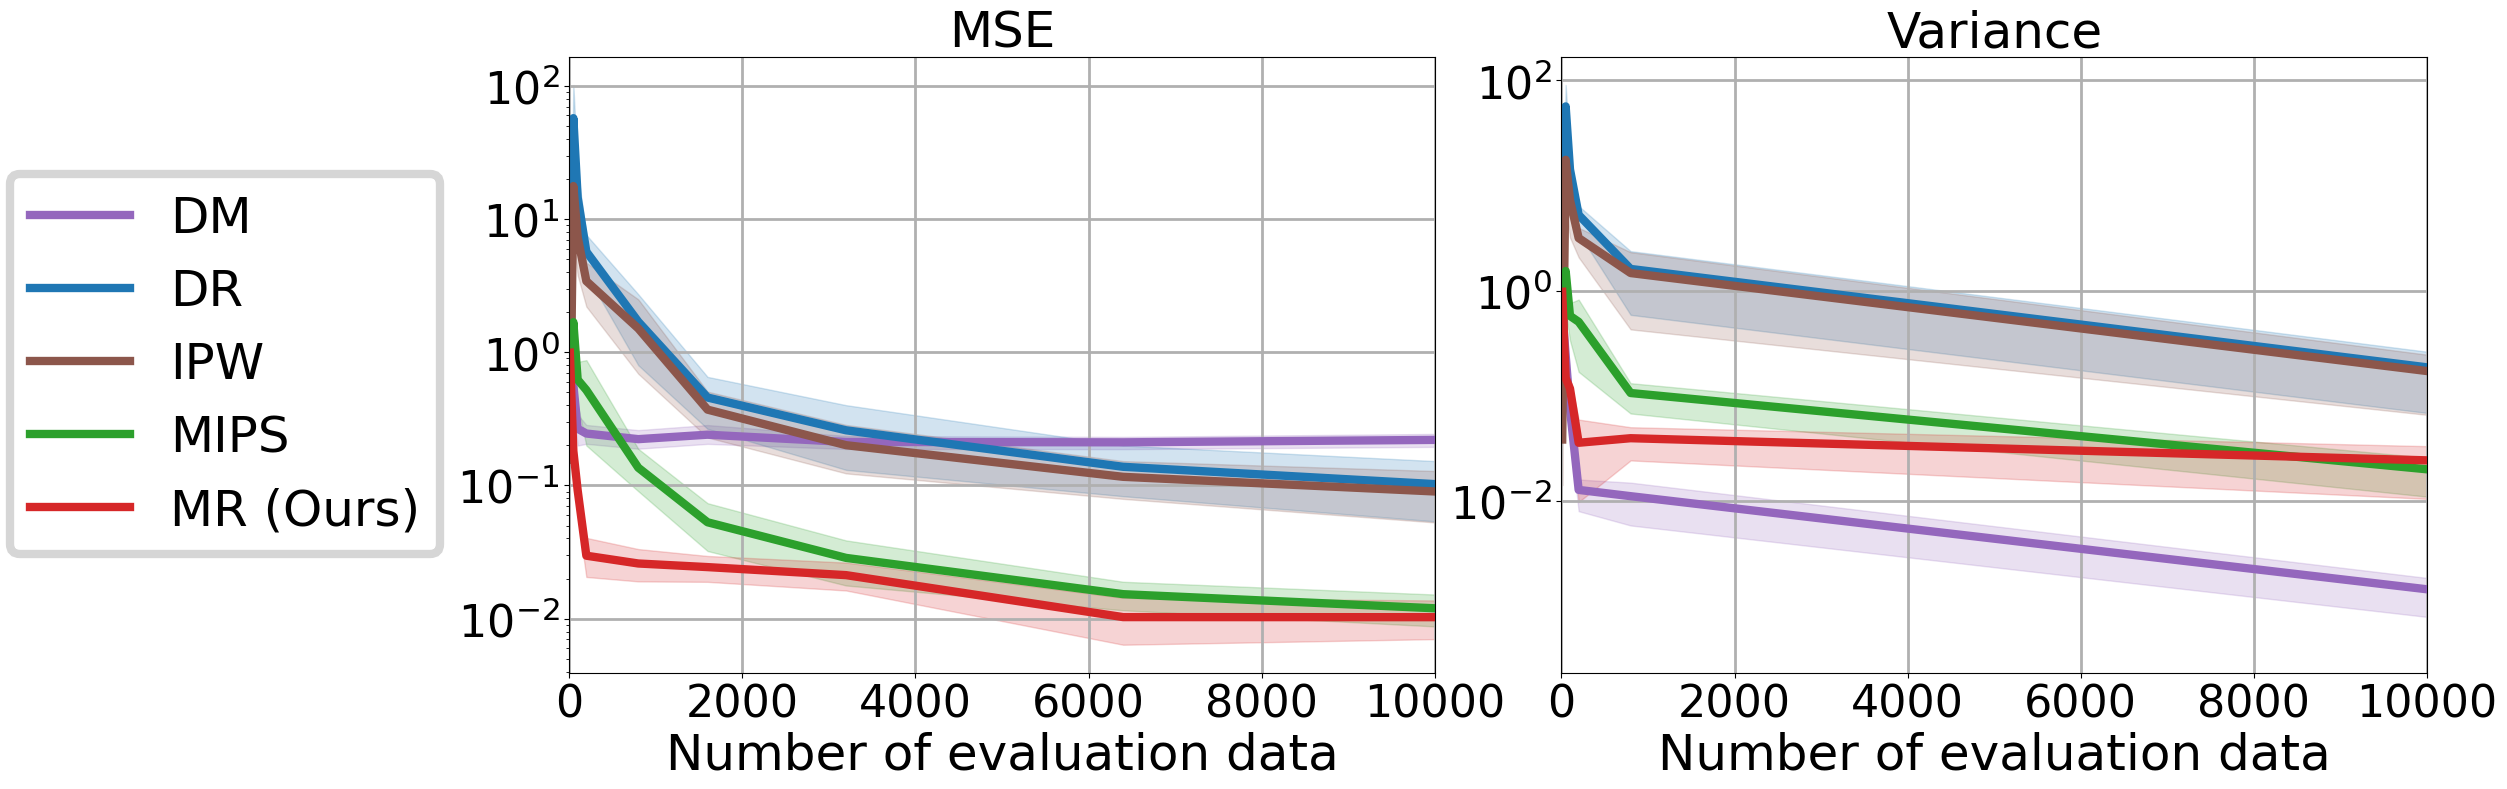
\includegraphics[height=1.06in]{figures/mr/ope_vs_neval_nac_100_alphatar_0_8_dimc_1000_untrunc.png}
         \caption{Results with varying evaluation data size $n$.}
         \label{fig:mse-vs-neval}
     \end{subfigure}%
     \begin{subfigure}[b]{0.5\textwidth}
         \centering
         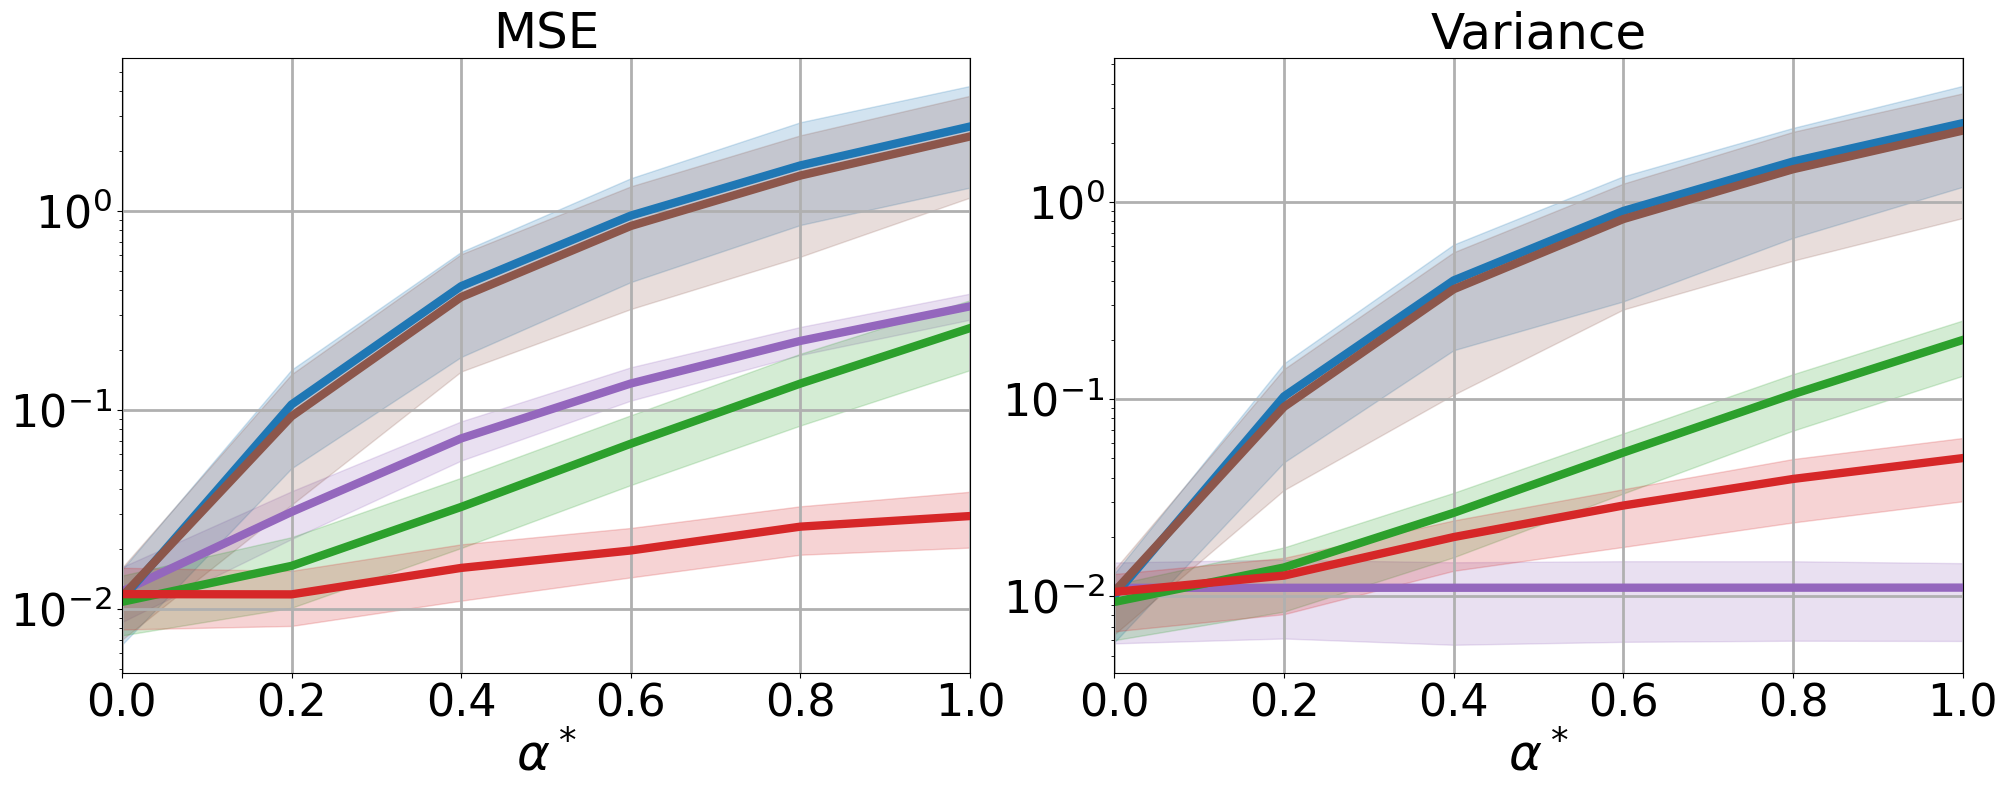
\includegraphics[height=1.06in]{figures/mr/ope_vs_alphatar_nac_100_neval_800_dimc_1000.png}
         \caption{Results with varying $\alpha^\ast$.}
         \label{fig:mse-vs-betatar}
     \end{subfigure}\\
    \caption{Results for synthetic data experiment. In \ref{fig:mse-vs-neval} we have $\alpha^\ast=0.8$ and in \ref{fig:mse-vs-betatar} we have $n = 800$.}
    \label{fig:syn_results1}
\end{figure}

% \begin{figure}[t]
%      \centering
%      \begin{subfigure}[b]{1\textwidth}
%          \centering
%          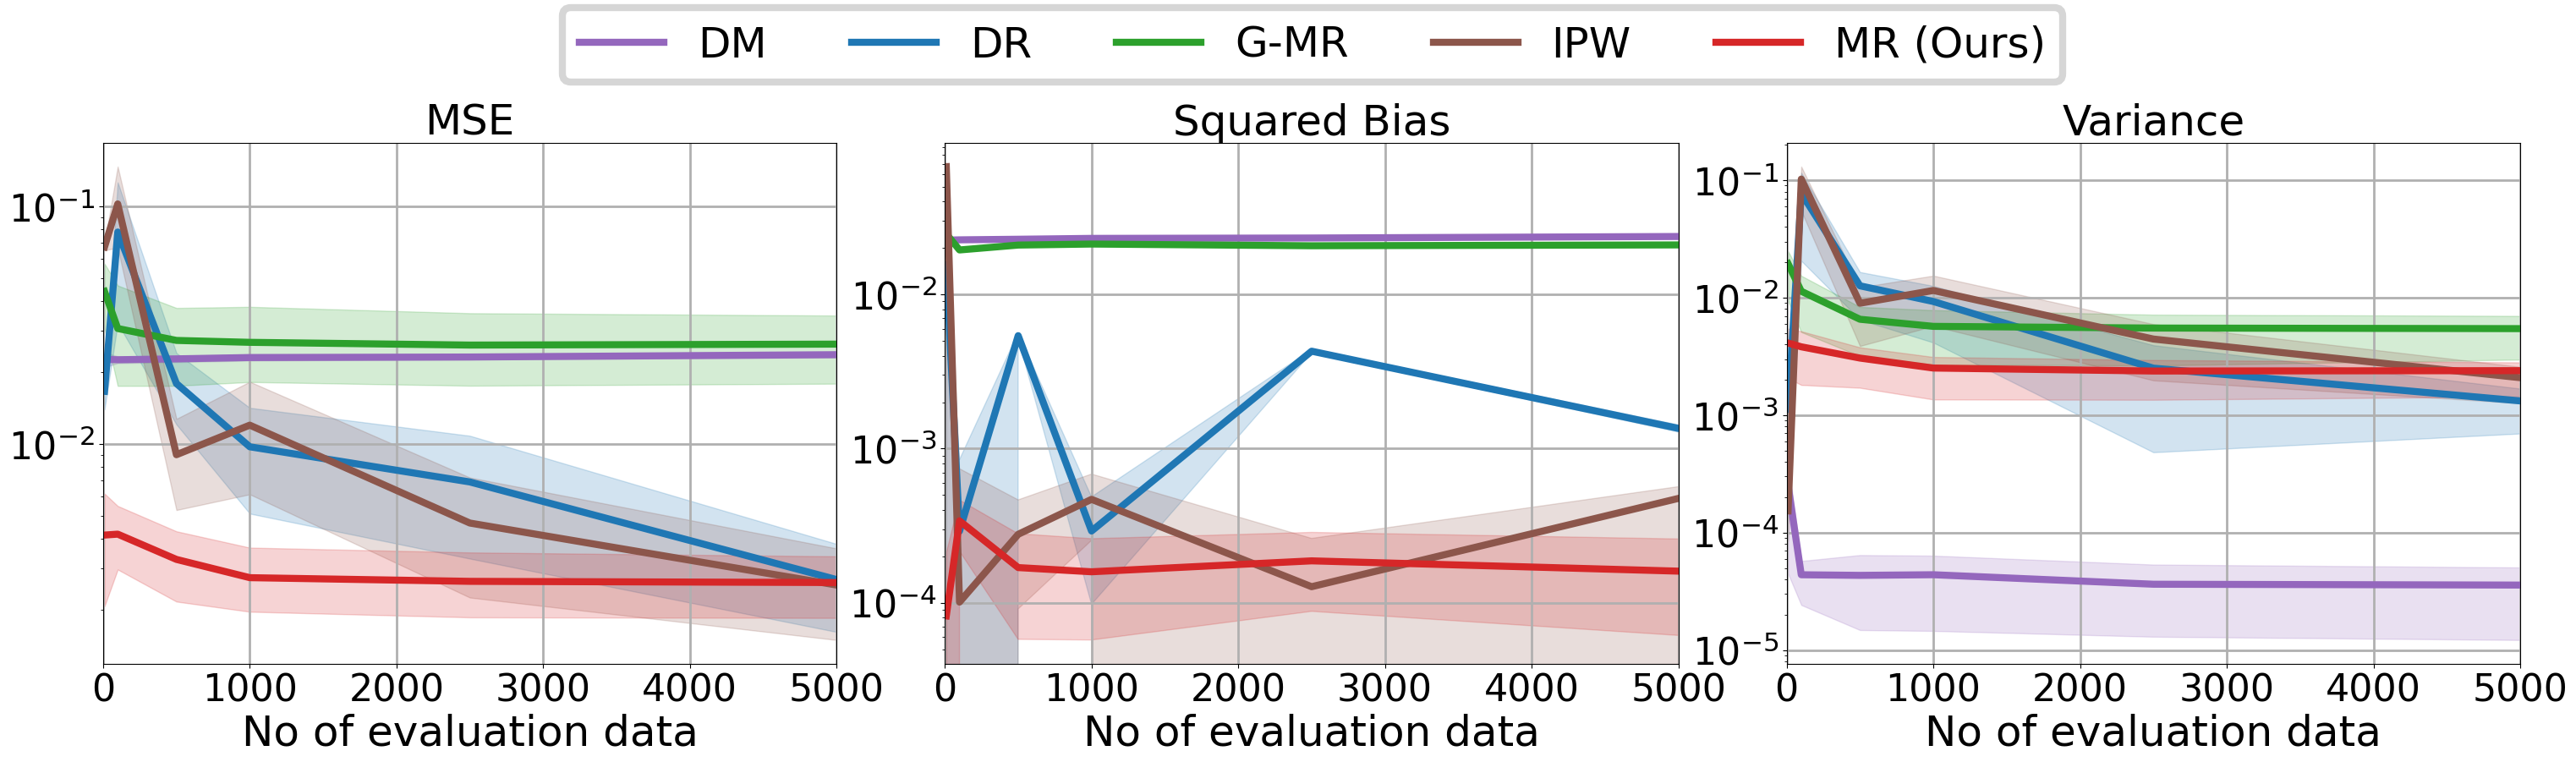
\includegraphics[width=0.75\textwidth]{figures/mr/ope_vs_neval_nac_100_alphatar_0_8_dimc_100_ntrain_100000.png}
%          \caption{Results with varying size of evaluation dataset $n$ for $\alpha^\ast = 0.8$.}
%          \label{fig:mse-vs-neval}
%      \end{subfigure}\\
%      \begin{subfigure}[b]{1\textwidth}
%          \centering
%          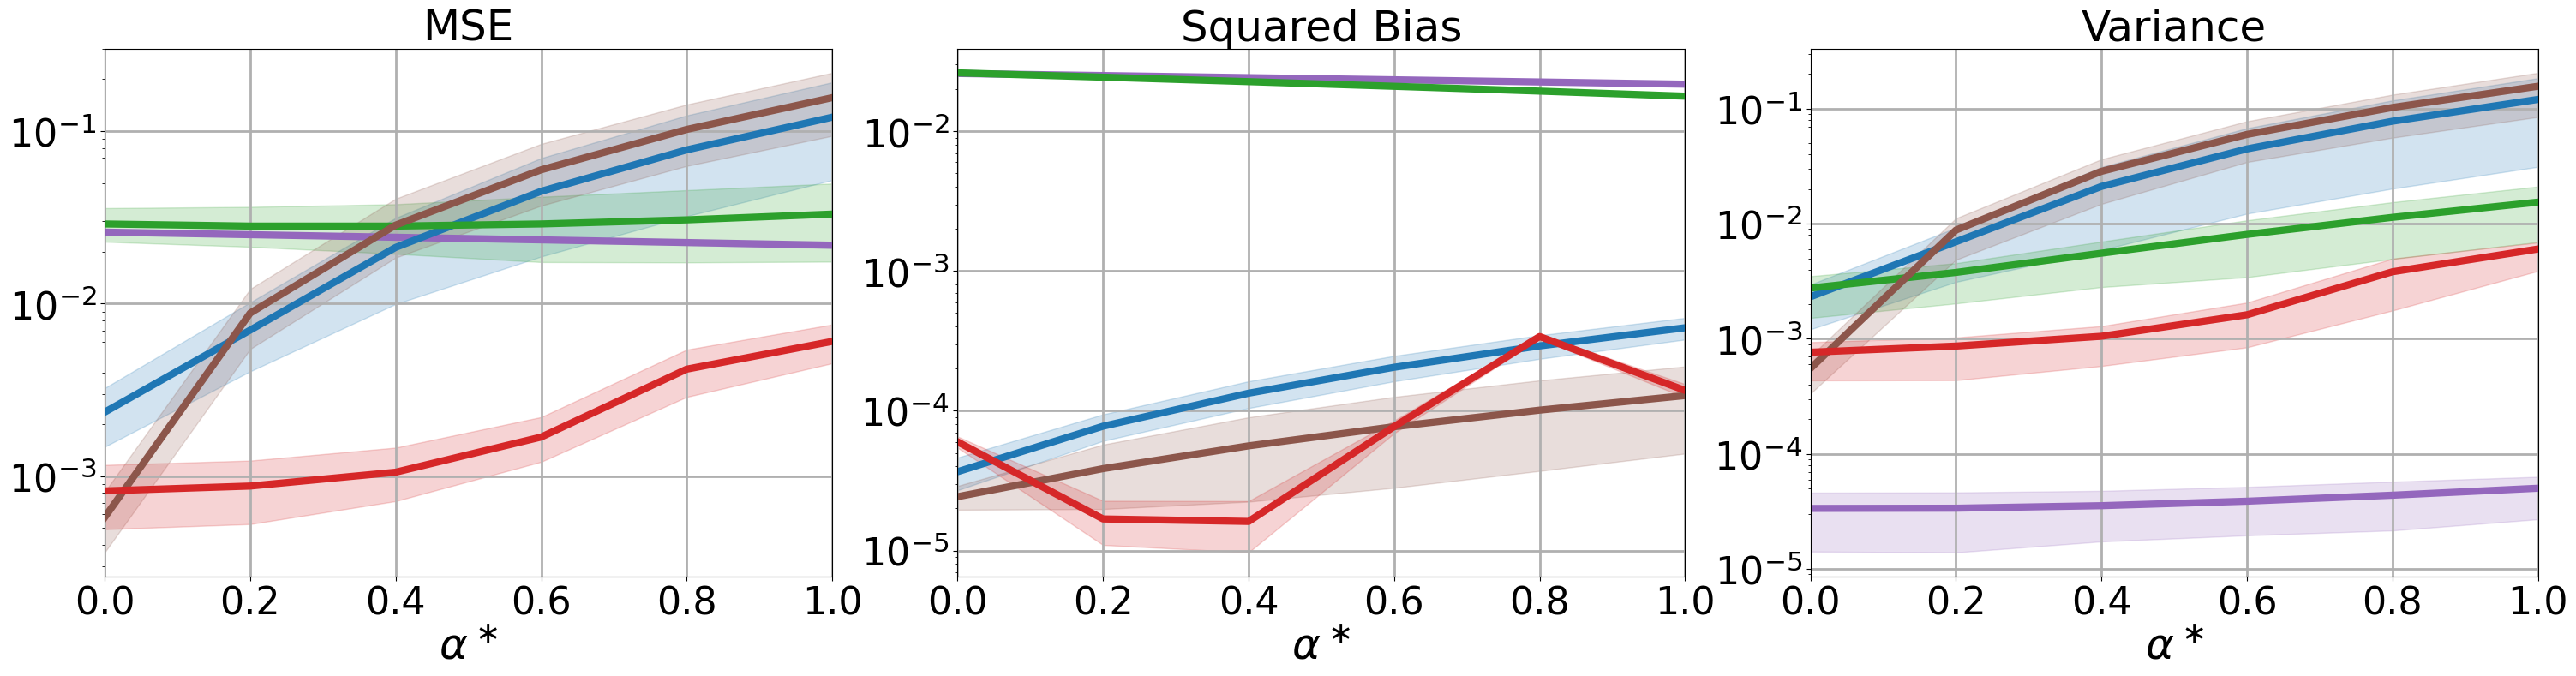
\includegraphics[width=0.75\textwidth]{figures/mr/ope_vs_alphatar_nac_100_neval_100_dimc_100_ntrain_100000.png}
%          \caption{Results with varying $\alpha^\ast$ for $n = 100$.}
%          \label{fig:mse-vs-betatar}
%      \end{subfigure}\\
%     \caption{Results with increasing $n$ and $\alpha^\ast$.}
%     \label{fig:syn_results1}
% \end{figure}
\myparagraph{Results}
We compute the target policy value using the $n$ evaluation datapoints. Here, the MSE of the estimators is computed over 10 different sets of logged data replicated with different seeds. The results presented have context dimension $d=1000$, number of actions $n_a=100$ and training data size $m=5000$. More experiments for a variety of parameter values are included in Appendix \ref{subsec:mips-empirical}.


% \begin{figure}
%      \centering
%      \begin{subfigure}[b]{1\textwidth}
%          \centering
%          \includegraphics[width=\textwidth]{figures/mr/latest/ope_vs_neval_nac_100_alphatar_0.2_dimc_100_ntrain_100000.png}
%          \caption{Results with varying size of evaluation dataset $n$ for $d=100$, $n_{a}=100$, $\alpha^\ast = 0.2$.}
%          \label{fig:mse-vs-neval}
%      \end{subfigure}\\
%      \begin{subfigure}[b]{1\textwidth}
%          \centering
%          \includegraphics[width=\textwidth]{figures/mr/latest/ope_vs_alphatar_dimc_100_nac_100_neval_100_ntrain_10000.png}
%          \caption{Results with varying $\alpha^\ast$ for $d=100$, $n_{a}=100$, $n = 100$.}
%          \label{fig:mse-vs-betatar}
%      \end{subfigure}\\
%      \begin{subfigure}[b]{1\textwidth}
%          \centering
%          \includegraphics[width=\textwidth]{figures/mr/latest/ope_vs_dimc_nac_100_alphatar_0.2_neval_100_ntrain_100000.png}
%          \caption{Results with varying context dimensions $d$ for $n_{a}=100$, $n = 100$, $\alpha^\ast = 0.2$.}
%          \label{fig:mse-vs-d}
%      \end{subfigure}\\
%      \begin{subfigure}[b]{1\textwidth}
%          \centering
%          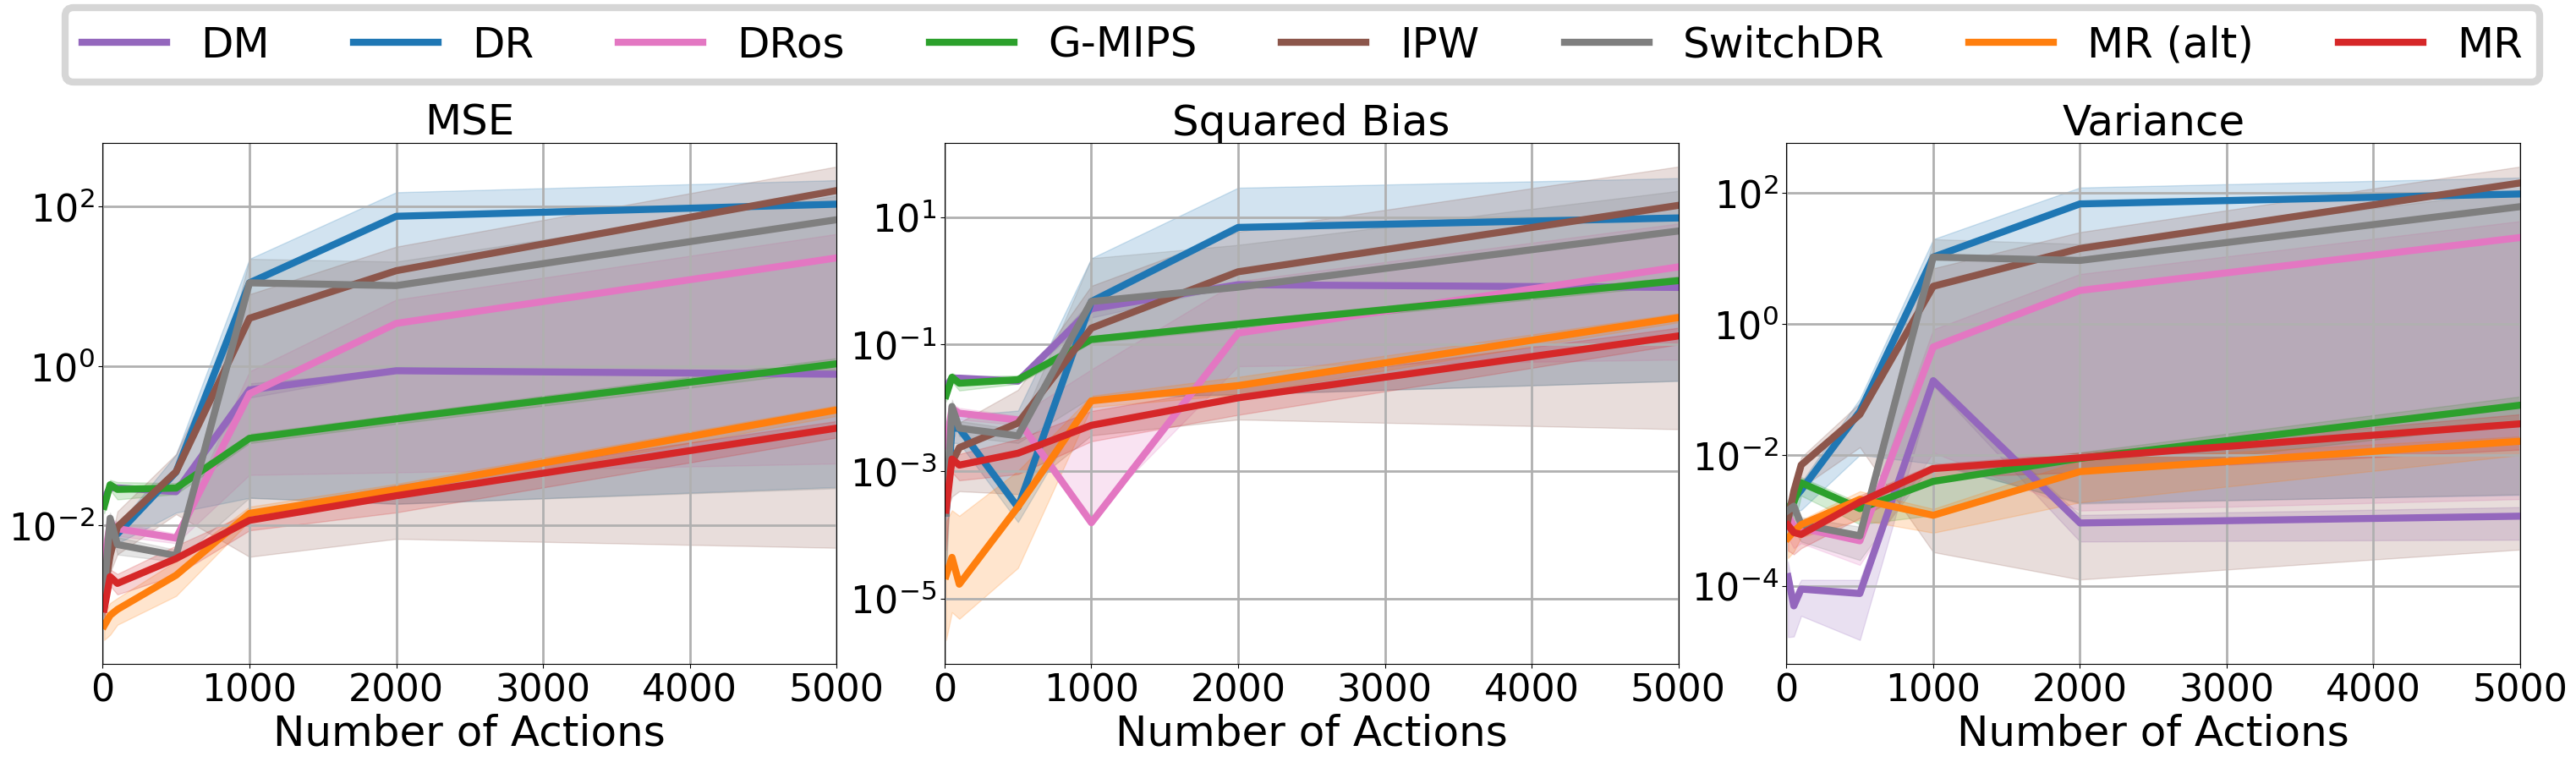
\includegraphics[width=\textwidth]{figures/mr/latest/ope_vs_nac_dimc_100_alphatar_0.2_neval_100_ntrain_100000.png}
%          \caption{Results with varying number of actions $n_{a}$ for $d=100$, $n = 100$, $\alpha^\ast = 0.2$.}
%          \label{fig:mse-vs-nac}
%      \end{subfigure}
%         \caption{Results for synthetic data experiments}
%         \label{fig:syn_results}
% \end{figure}

\myparagraph{Varying number of evaluation data $n$} 
In Figure \ref{fig:mse-vs-neval} we plot the results with increasing size of evaluation data $n$ increases. MR achieves the smallest MSE among all the baselines considered when $n$ is small, with the MSE of MR being at least an order of magnitude smaller than every baseline for $n\leq 500$. This shows that MR is significantly more accurate than the baselines when the size of the evaluation data is small. As $n\rightarrow \infty$, the difference between the results for MR and MIPS decreases. However, MR attains smaller variance and MSE than MIPS generally, verifying our analysis in Section \ref{subsec:mips-comparison}.
% IPW and DR become increasingly accurate because of their consistency and therefore the difference between MR and these baselines becomes less pronounced. 
% Additionally, it can be seen that the MR estimator also achieves the smallest squared bias overall. 
% In contrast, G-MR has a high squared bias as a result of the estimation error of the marginal ratio $\ptar(r)/\pbeh(r)$, which is more difficult to estimate the marginal ratio $\ptar(y)/\pbeh(y)$ as $r$ is two dimensional. The variance of G-MR estimator, on the other hand, is smaller than that of IPW when $n < 2000$, as suggested by Proposition \ref{prop:mips_var_reduction}.
Moreover, Figure \ref{fig:mse-vs-neval} shows that while the variance of MR is greater than that of DM, it still achieves the lowest MSE overall, owing to the high bias of DM.

\begin{wrapfigure}{r}{0.35\textwidth}
    \centering
    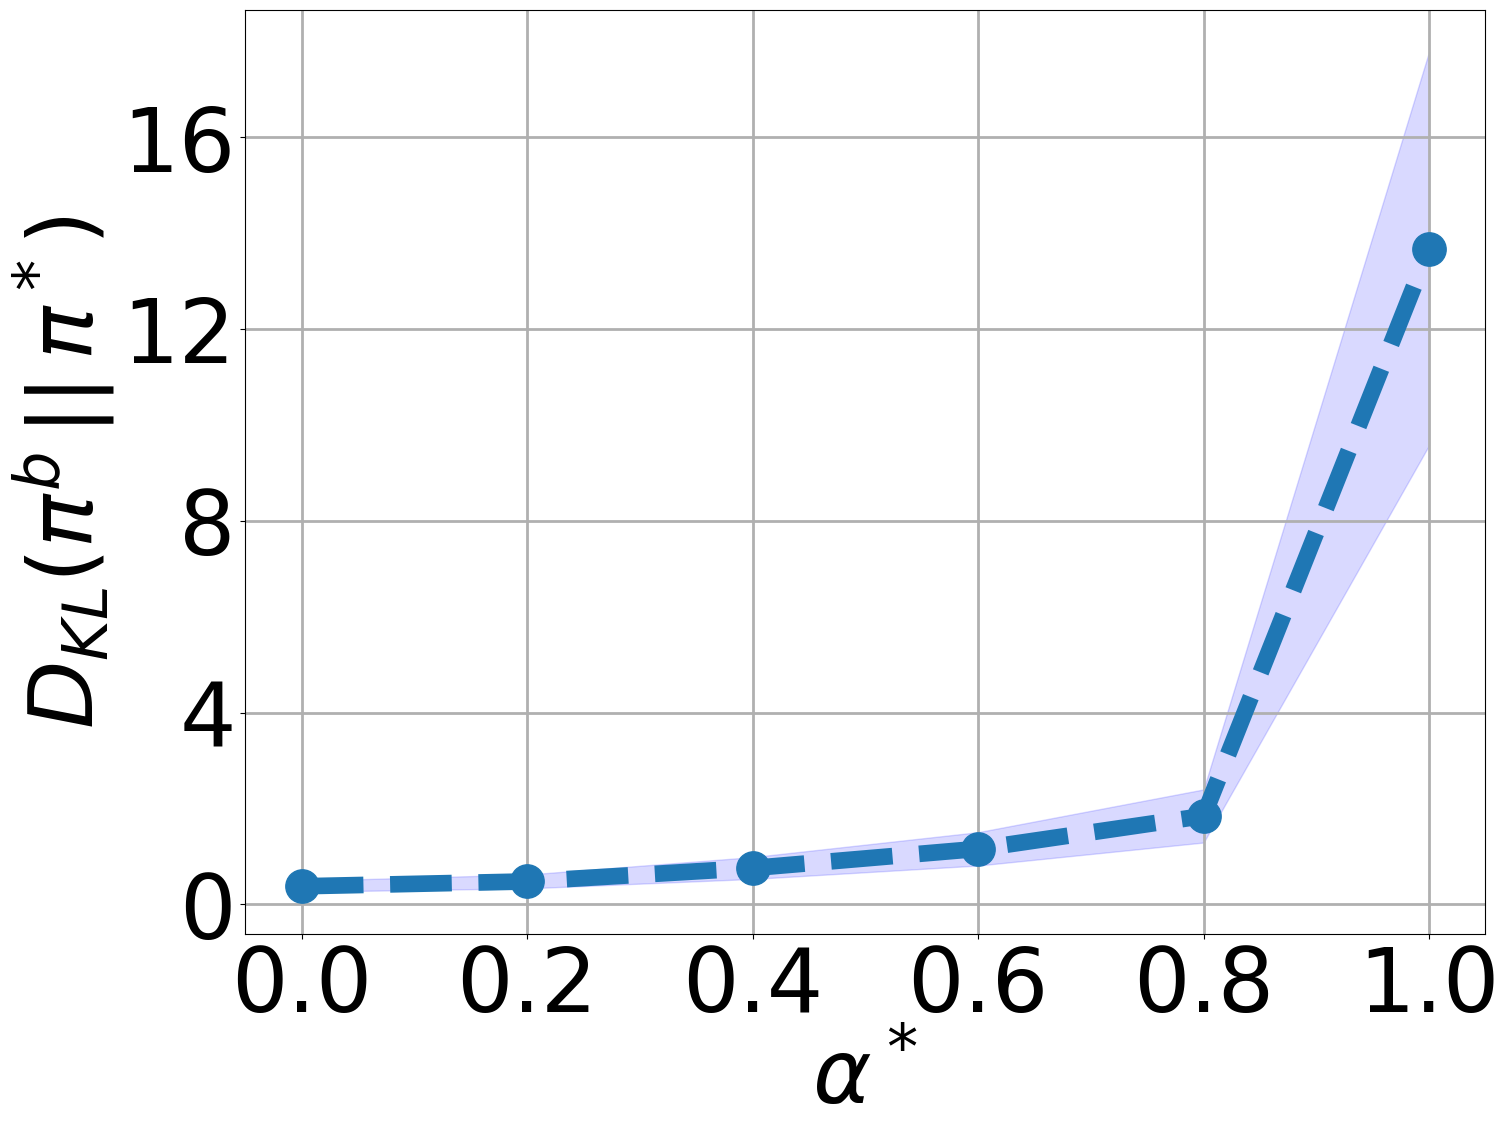
\includegraphics[width=0.35\textwidth]{figures/mr/kl-divergence-w-uncertainty.png}
    % \vspace{-0.75cm}
    % \caption{$D_{\textup{KL}}(\beh \,||\, \tar)$ with increasing $\alpha^\ast$}
    % \label{fig:kl-div-synthetic-data}
\end{wrapfigure}
\myparagraph{Varying $\alpha^\ast$}
As $\alpha^\ast$ parameter of the target policy increases, so does the shift between the policies $\beh$ and $\pi^{\alpha^\ast}$ as illustrated by the figure on the right, which plots the KL-divergence $D_{\textup{KL}}(\beh\, || \, \pi^{\alpha^\ast})$ as a function of $\alpha$.
% To analyse the shift between the policies $\beh$ and $\pi^{\alpha^\ast}$, the figure on the right plots the KL-divergence between the two policies as $\alpha^\ast$ increases. 
% \ref{fig:kl-div-synthetic-data}. 
% The figure shows that the shift between target and behaviour policies increases with increasing $\alpha^\ast$.
Figure \ref{fig:mse-vs-betatar} plots the results for increasing policy shift. 
Overall, the MSE of MR estimator is lowest among all the baselines. Moreover, while the MSE and variance of all estimators increase with increasing $\alpha^\ast$ the increase in these quantities is lower for the MR estimator than for the other baselines. Therefore, the relative performance of MR estimator improves with increasing policy shift and MR remains robust to increase in policy shift.
% It can be seen that the MSE of MR remains roughly the same with increasing $\alpha^\ast$, whereas the MSE of all other baselines increases. Moreover, both the squared bias and variance of the MR estimator becomes comparatively better than those of other baselines as the policy shift increases. 
% While the MSE and variances of all baselines increases with increasing $\beta^\ast$, the MSE and variance of MR estimator remains relatively small. Moreover, while the MSE of DM does not change noticeably with changing  $\beta^\ast$, it is still at least 2 orders of magnitude larger than that of MR. 
% This shows that MR remains significantly robust to increase in policy shift, relative to the other baselines.

\myparagraph{Additional ablation studies}
In Appendix \ref{subsec:mips-empirical}, we investigate the effect of varying context dimensions $d$, number of actions $n_a$ and number of training data $m$. In every case, we observe that the MR estimator has a smaller MSE than all other baselines considered. In particular, MR remains robust to increasing $n_a$ whereas the MSE and variance of IPW and DR estimators degrade substantially when $n_a \geq 2000$. Likewise, MR outperforms the baselines even when the training data size $m$ is small.

% \begin{figure}[t]
%      \centering
%      \begin{subfigure}[b]{0.5\textwidth}
%          \centering
%          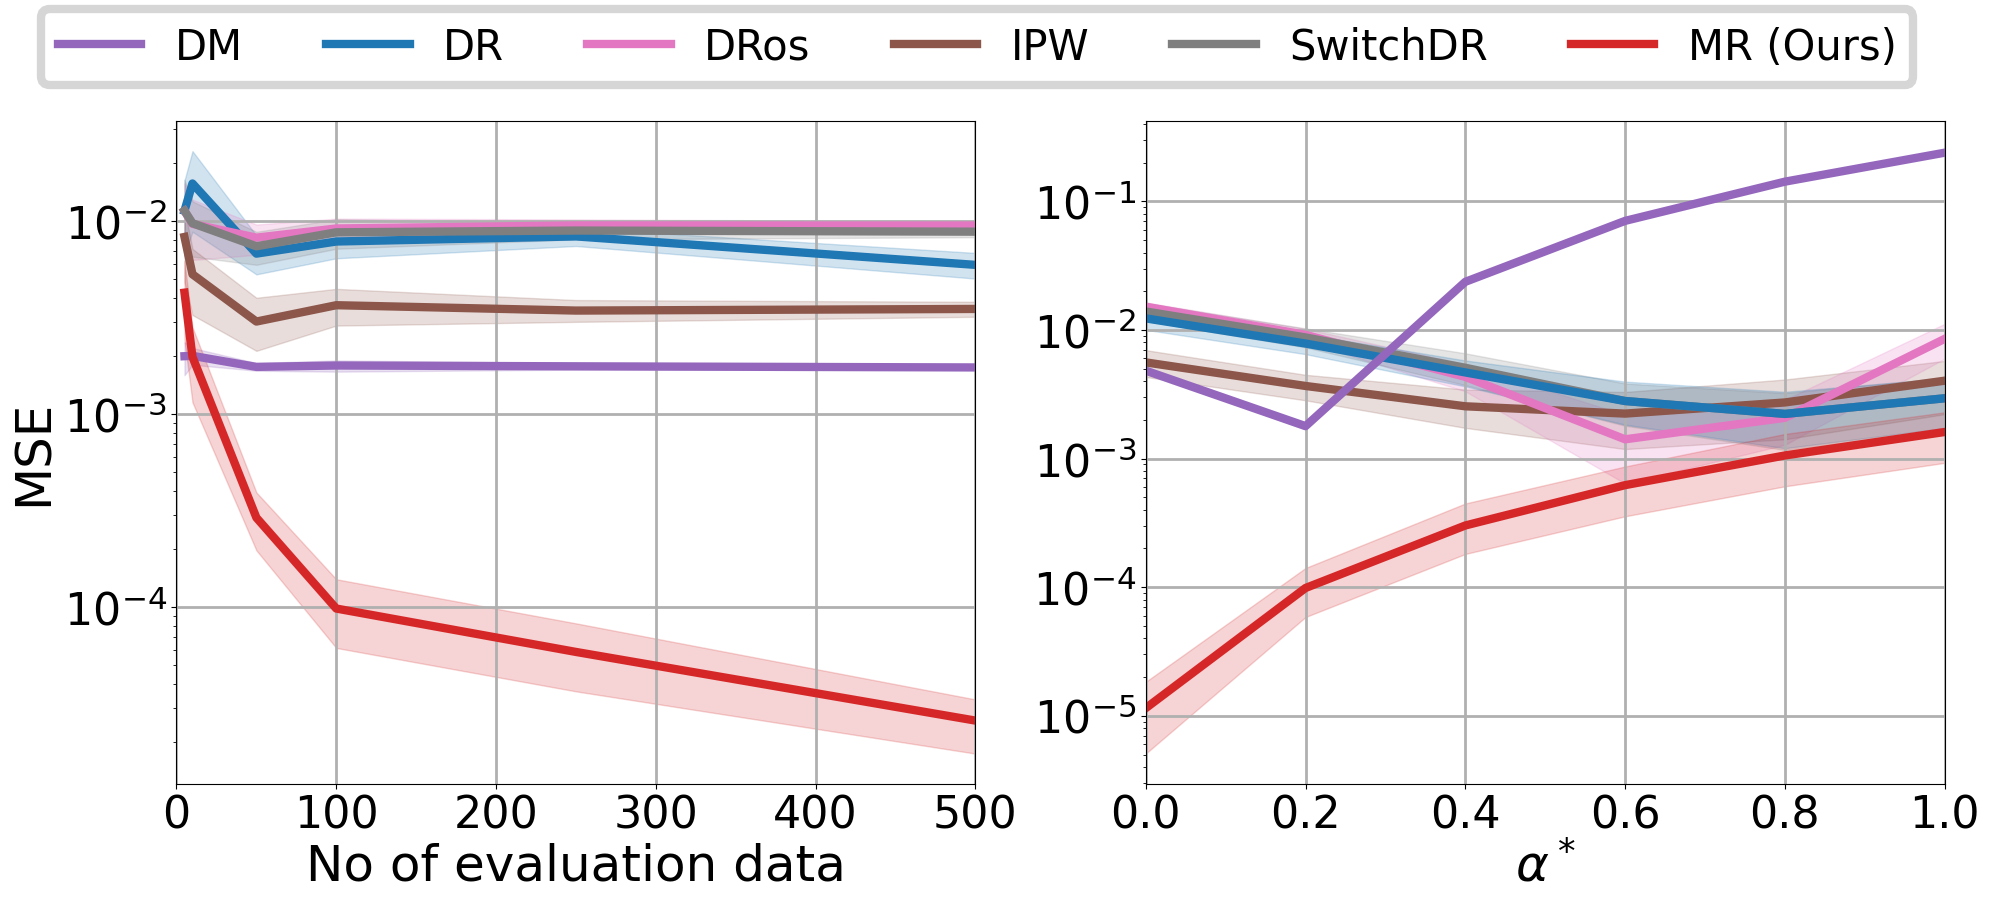
\includegraphics[height=0.92in]{figures/mr/pendigits_main.png}
%          \caption{Results for PenDigits dataset}
%          \label{fig:pendigits-main}
%      \end{subfigure}%
%      \begin{subfigure}[b]{0.5\textwidth}
%          \centering
%          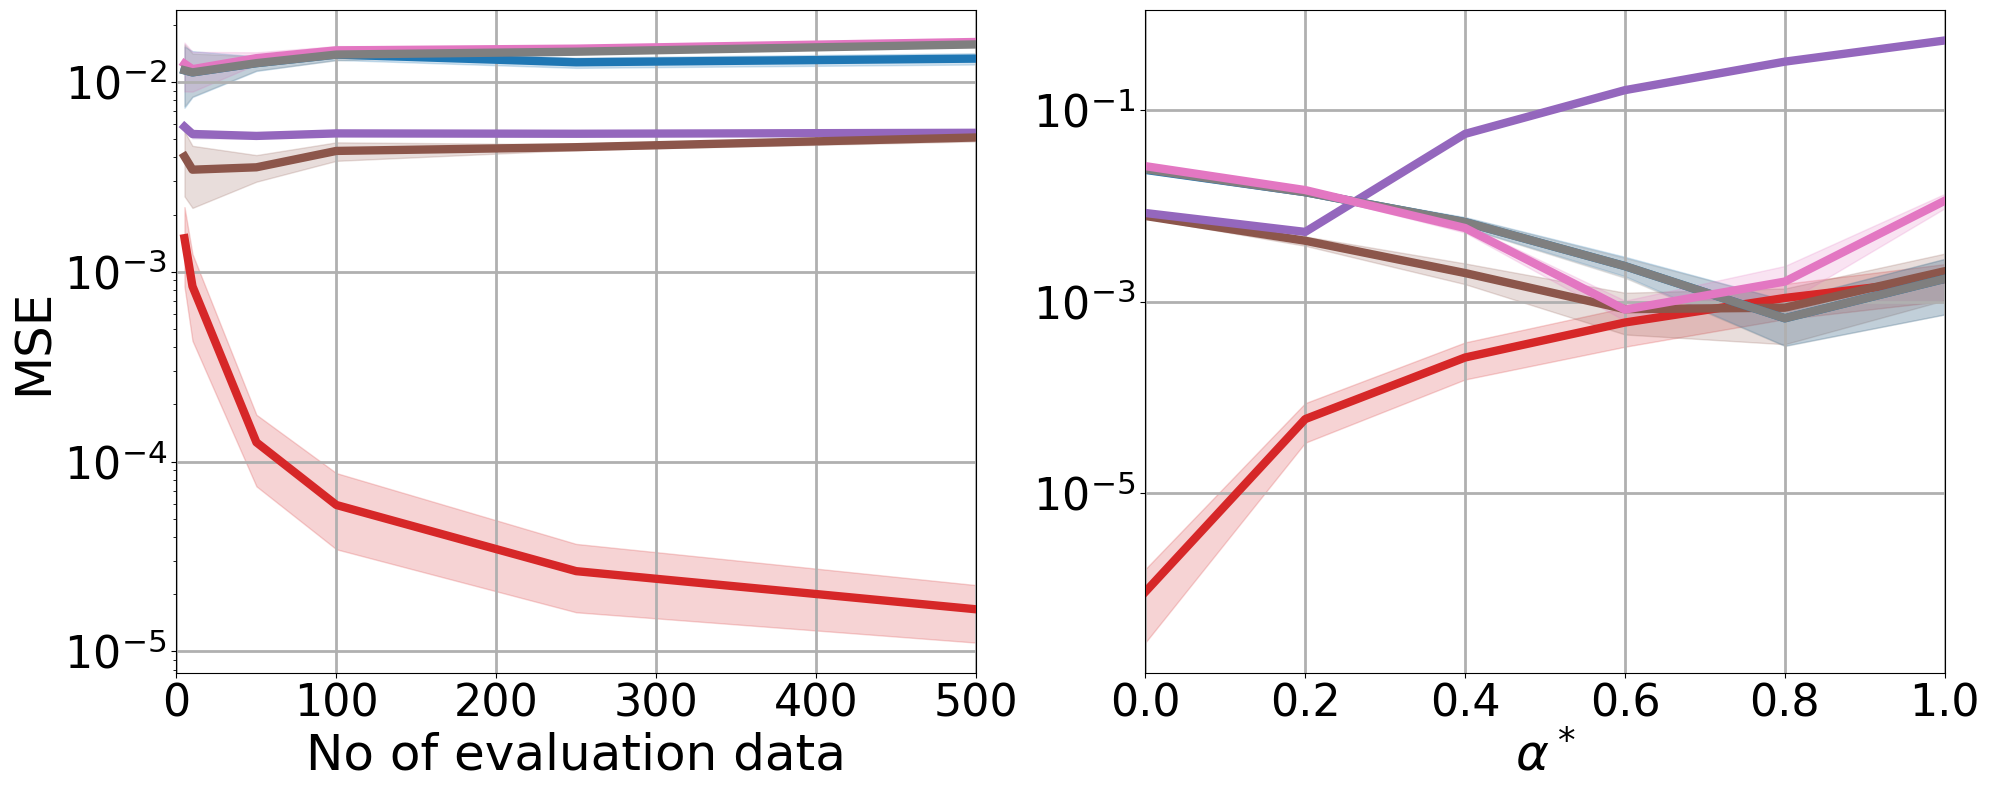
\includegraphics[height=0.92in]{figures/mr/mnist_main.png}
%          \caption{Results for mnist dataset.}
%          \label{fig:mnist-main}
%      \end{subfigure}\\
%     \caption{Results for synthetic data experiment. In \ref{fig:mse-vs-neval} we have $\alpha^\ast=0.8$ and in \ref{fig:mse-vs-betatar} we have $n = 100$.}
%     \label{fig:multiclass-main}
% \end{figure}
% \begin{table}[t]
%     \centering
%     \caption{Mean squared error of target policy value with standard errors over 10 different seeds for different classification datasets. Here, number of evaluation data $n=100$, and $\alpha^\ast=0.2$.}
%     \label{tab:classification-dataset-results}
%     \begin{tiny}
% \begin{tabular}{lllllll}
% \toprule
% Dataset & Digits & Letter & Mnist & OptDigits & PenDigits & SatImage \\
% \midrule
% DM & 0.00505$\pm$0.00016 & 0.01255$\pm$0.00011 & 0.00536$\pm$0.00009 & 0.00240$\pm$0.00009 & 0.00179$\pm$0.00011 & 0.00114$\pm$0.00005 \\
% DR & 0.01768$\pm$0.00058 & 0.00279$\pm$0.00093 & 0.01394$\pm$0.00084 & 0.00590$\pm$0.00089 & 0.00784$\pm$0.00128 & 0.02249$\pm$0.00660 \\
% DRos & 0.01721$\pm$0.00054 & 0.00281$\pm$0.00070 & 0.01467$\pm$0.00068 & 0.00788$\pm$0.00055 & 0.00916$\pm$0.00100 & 0.02160$\pm$0.00237 \\
% IPW & 0.00523$\pm$0.00030 & 0.00142$\pm$0.00062 & 0.00433$\pm$0.00044 & 0.00197$\pm$0.00035 & 0.00367$\pm$0.00077 & 0.01292$\pm$0.00455 \\
% SwitchDR & 0.01768$\pm$0.00058 & 0.00310$\pm$0.00087 & 0.01394$\pm$0.00084 & 0.00709$\pm$0.00054 & 0.00875$\pm$0.00135 & 0.02035$\pm$0.00289 \\
% MR (Ours) & \textbf{0.00011$\pm$0.00002} & \textbf{0.00020$\pm$0.00002} & \textbf{0.00006$\pm$0.00002} & \textbf{0.00025$\pm$0.00009} & \textbf{0.00010$\pm$0.00004} & \textbf{0.00014$\pm$0.00004} \\
% \bottomrule
% \end{tabular}
% \end{tiny}
% \end{table}
% \begin{table}[!htp]
%     \centering
%     \caption{Mean squared error of target policy value with standard errors over 10 different seeds for different classification datasets. Here, number of evaluation data $n=100$, and $\alpha^\ast=0.2$.}
%     \label{tab:classification-dataset-results}
%     \begin{tiny}
% \begin{tabular}{lllllll}
% \toprule
% Dataset & Digits & Letter & OptDigits & PenDigits & SatImage & Mnist \\
% \midrule
% DM & 0.00505$\pm$0.00016 & 0.01255$\pm$0.00011 & 0.00240$\pm$0.00009 & 0.00179$\pm$0.00011 & 0.00114$\pm$0.00005 & 0.00536$\pm$0.00009 \\
% DR & 0.01768$\pm$0.00058 & 0.00279$\pm$0.00093 & 0.00590$\pm$0.00089 & 0.00784$\pm$0.00128 & 0.02249$\pm$0.00660 & 0.01394$\pm$0.00084\\
% DRos & 0.01721$\pm$0.00054 & 0.00281$\pm$0.00070 & 0.00788$\pm$0.00055 & 0.00916$\pm$0.00100 & 0.02160$\pm$0.00237 & 0.01467$\pm$0.00068\\
% IPW & 0.00523$\pm$0.00030 & 0.00142$\pm$0.00062 & 0.00197$\pm$0.00035 & 0.00367$\pm$0.00077 & 0.01292$\pm$0.00455 & 0.00433$\pm$0.00044\\
% SwitchDR & 0.01768$\pm$0.00058 & 0.00310$\pm$0.00087 & 0.00709$\pm$0.00054 & 0.00875$\pm$0.00135 & 0.02035$\pm$0.00289 & 0.01394$\pm$0.00084\\
% MR (Ours) & \textbf{0.00011$\pm$0.00002} & \textbf{0.00020$\pm$0.00002} & \textbf{0.00025$\pm$0.00009} & \textbf{0.00010$\pm$0.00004} & \textbf{0.00014$\pm$0.00004} & \textbf{0.00006$\pm$0.00002}\\
% \bottomrule
% \end{tabular}
% \end{tiny}
% \end{table}
% \vspace{-5mm}
\begin{sidewaystable}[!htp]
    \centering
    \caption{Mean squared error of target policy value with standard errors over 10 different seeds for different classification datasets. Here, number of evaluation data $n=1000$, and $\alpha^\ast=0.6$.}
    \label{tab:classification-dataset-results}
    \begin{footnotesize}
    \begin{scshape}
% \begin{tabular}{lllllll}
% \toprule
% Dataset & Digits & Letter & OptDigits & PenDigits & SatImage & Mnist\\
% \midrule
% DM & 0.16053$\pm$0.00263 & 0.11686$\pm$0.00108 & 0.05963$\pm$0.00129 & 0.05889$\pm$0.00180 & 0.02165$\pm$0.00125 & 0.12556$\pm$0.00112 \\
% DR & 0.05694$\pm$0.00412 & 0.67369$\pm$0.31527 & 0.03697$\pm$0.00707 & 0.20803$\pm$0.13579 & 0.06484$\pm$0.04971 & 0.16665$\pm$0.01689 \\
% DRos & 0.03180$\pm$0.00231 & 0.05629$\pm$0.02057 & 0.00928$\pm$0.00181 & 0.00698$\pm$0.00236 & 0.00824$\pm$0.00212 & 0.06950$\pm$0.00549 \\
% IPW & 0.06465$\pm$0.00459 & 0.96803$\pm$0.44189 & 0.05451$\pm$0.00875 & 0.02769$\pm$0.00720 & 0.02298$\pm$0.00903 & 0.20363$\pm$0.02123 \\
% SwitchDR & 0.05694$\pm$0.00412 & 0.11881$\pm$0.02220 & 0.04086$\pm$0.00711 & 0.02150$\pm$0.00569 & 0.01677$\pm$0.00598 & 0.16665$\pm$0.01689 \\
% MR (Ours) & \textbf{0.00169$\pm$0.00032} & \textbf{0.00126$\pm$0.00045} & \textbf{0.00115$\pm$0.00040} & \textbf{0.00261$\pm$0.00062} & \textbf{0.00314$\pm$0.00071} & \textbf{0.00654$\pm$0.00092} \\
% \bottomrule
% \end{tabular}

\begin{tabular}{llllllll}
\toprule
Dataset &             Digits &               Letter &          OptDigits &          PenDigits &           SatImage  &              Mnist & CIFAR-100\\
\midrule
DM        &  0.1508$\pm$0.0015 &    0.0886$\pm$0.0026 &  0.0485$\pm$0.0016 &   0.0520$\pm$0.0016 &  0.0208$\pm$0.0009  &  0.1109$\pm$0.0014 & 0.0020$\pm$0.0001 \\
DR        &    0.1334$\pm$0.0400 &    \red{35.085$\pm$17.768} &  0.0464$\pm$0.0061 &  0.2343$\pm$0.1404 &   0.0560$\pm$0.0395 &  0.2617$\pm$0.0139 & \red{3823.9$\pm$2023.2} \\
DRos      &  0.0847$\pm$0.0025 &    0.2363$\pm$0.0586 &  0.0384$\pm$0.0025 &  0.0138$\pm$0.0029 &  0.0078$\pm$0.0008 &  0.2151$\pm$0.0061 & 0.2628$\pm$0.1087 \\
IPW       &  0.1632$\pm$0.0462 &  \red{45.253$\pm$22.057} &   0.0844$\pm$0.0056 &  0.1342$\pm$0.0531 &    0.0900$\pm$0.0676 & 0.3359$\pm$0.0118 & \red{4116.9$\pm$2097.9}\\
SwitchDR  &  0.0982$\pm$0.0032 &    0.2387$\pm$0.0507 &  0.0557$\pm$0.0047 &   0.0342$\pm$0.0090 &  0.0136$\pm$0.0012  &   0.2750$\pm$0.0102 & 1.1644$\pm$0.8227 \\
MR (Ours) &  \textbf{0.0034$\pm$0.0001} &    \textbf{0.0018$\pm$0.0004} &  \textbf{0.0006$\pm$0.0002} &  \textbf{0.0008$\pm$0.0002} &  \textbf{0.0016$\pm$0.0003} &  \textbf{0.0121$\pm$0.0009} &  \textbf{0.0007$\pm$0.0002}\\
\bottomrule
\end{tabular}

% \begin{tabular}{lllllll}
% \toprule
% Dataset & Digits & Letter & OptDigits & PenDigits & SatImage & Mnist\\
% \midrule
% DM & 0.161$\pm$0.003 & 0.117$\pm$0.001 & 0.060$\pm$0.001 & 0.059$\pm$0.002 & 0.022$\pm$0.001 & 0.126$\pm$0.001 \\
% DR & 0.057$\pm$0.004 & 0.674$\pm$0.315 & 0.037$\pm$0.007 & 0.208$\pm$0.136 & 0.065$\pm$0.050 & 0.167$\pm$0.017 \\
% DRos & 0.032$\pm$0.002 & 0.056$\pm$0.021 & 0.009$\pm$0.002 & 0.007$\pm$0.002 & 0.008$\pm$0.002 & 0.070$\pm$0.005 \\
% IPW & 0.065$\pm$0.005 & 0.968$\pm$0.442 & 0.055$\pm$0.009 & 0.028$\pm$0.007 & 0.023$\pm$0.009 & 0.204$\pm$0.021 \\
% SwitchDR & 0.057$\pm$0.004 & 0.118$\pm$0.022 & 0.041$\pm$0.007 & 0.022$\pm$0.006 & 0.017$\pm$0.006 & 0.167$\pm$0.017 \\
% MR (Ours) & \textbf{0.002$\pm$0.001} & \textbf{0.001$\pm$0.001} & \textbf{0.001$\pm$0.001} & \textbf{0.003$\pm$0.001} & \textbf{0.003$\pm$0.001} & \textbf{0.007$\pm$0.001} \\
% \bottomrule
% \end{tabular}
\end{scshape}
\end{footnotesize}
\end{sidewaystable}
\subsection{Experiments on classification datasets}
Following previous works on OPE in contextual bandits \citep{dudik2014doubly, kallus2021optimal, mehrdad2018more,wang2017optimal}, we transform classification datasets into contextual bandit feedback data in this experiment.
We consider five UCI classification datasets \citep{dua2019uci} as well as Mnist \citep{deng2012mnist} and CIFAR-100 \citep{krizhevsky2009learning} datasets, each of which comprises $\{(x_i, a^\gt_i)\}_{i}$, where $x_i\in \Xspace$ are feature vectors and $a^\gt_i\in \Aspace$ are the ground-truth labels.
% Here, the datasets considered include five UCI classification datasets \citep{dua2019uci}, as well as the mnist dataset \citep{deng2012mnist}. 
% Following previous works \citep{dudik2014doubly, kallus2021optimal, mehrdad2018more,wang2017optimal}, the classification datasets are transformed to contextual bandit feedback data. 
In the contextual bandits setup, the feature vectors $x_i$ are considered to be the contexts, whereas the actions correspond to the possible class of labels. For the context vector $x_i$ and the action $a_i$, the reward $y_i$ is defined as $y_i \coloneqq \ind(a_i = a^\gt_i)$, i.e., the reward is 1 when the action is the same as the ground truth label and 0 otherwise. Here, the baselines considered include the DM, IPW and DR estimators as well as Switch-DR \citep{wang2017optimal} and DR with Optimistic Shrinkage (DRos) \citep{su2020doubly}. We do not consider a MIPS baseline here as there is no natural embedding $E$ of $A$. Additional details are provided in Appendix \ref{subsec:additional-experiments-classification}. 
% regarding the behaviour and target policies and the estimation of weights are provided in Appendix \ref{sec:app-additional-results}. 
% Similar to the synthetic data experiments, we define a class of parametric target policies parameterised by $\alpha^\ast \in [0, 1]$ (i.e., $\tar = \pi^{\alpha^\ast}$). 
% However, we show in Appendix \ref{subsec:additional-experiments} that in this case, the shift between target and behaviour policies increases as $\alpha^\ast \rightarrow 0$.

In Table \ref{tab:classification-dataset-results}, we present the results with number of evaluation data $n=1000$ and number of training data $m=500$. 
The table shows that across all datasets, MR achieves the lowest MSE among all methods. \flag{Moreover, for the Letter and CIFAR-100 datasets the IPW and DR yield large bias and variance arising from poor policy estimates $\hatbeh$. Despite this, the MR estimator which utilizes the \emph{same} $\hatbeh$ for the estimation of $\hat{w}(y)$ leads to much more accurate results.} We also verify that MR outperforms the baselines for increasing policy shift and evaluation data $n$ in Appendix \ref{subsec:additional-experiments-classification}.
% In fact, the MSE of MR is at least an order of magnitude lower than that of other methods.


% We provide extensive results for increasing policy shift and evaluation data size $n$ in Appendix \ref{sec:app-additional-results}.

% We split the dataset into training and testing datasets of sizes $m$ and $n$ respectively.

% \paragraph{Reward function}
% Let $X$ be a context with ground truth label $A^\gt$, we define the reward for action $A$ as:
% \[
% Y \coloneqq \ind(A = A^\gt).
% \]

\subsection{Application to ATE estimation}\label{subsec:causal-experiments}
% Further to our discussion regarding the application of MR for ATE estimation in Section \ref{subsec:application-to-causal-inference}, 
In this experiment, we investigate the empirical performance of the MR estimator for ATE estimation. 

\myparagraph{Twins dataset}
We use the Twins dataset studied in \cite{louizos2017causal}, which comprises data from twin births in the USA between 1989-1991. The treatment $a=1$ corresponds to being born the heavier twin and the outcome $Y$ corresponds to the mortality of each of the twins in their first year of life. Specifically, $Y(1)$ corresponds to the mortality of the heavier twin (and likewise for $Y(0)$). To simulate the observational study, we follow a similar strategy as in \cite{louizos2017causal} to selectively hide one of the two twins as explained in Appendix \ref{app:ate-empirical}. We obtain a total of 11,984 datapoints, of which 5000 datapoints are used to train the behaviour policy $\hatbeh$ and outcome model $\hat{q}(x, a)$.

% Here, the baselines considered include the DM, IPW and DR estimators as well as Switch-DR \citep{wang2017optimal} and DR with Optimistic Shrinkage (DRos) \citep{su2020doubly}. We do not consider a MIPS baseline here as there is no natural embedding $E$ of $A$. 
% Results for additional baselines have been given in Appendix \ref{app:ate-empirical}. 

% \begin{wraptable}{l}{0.55\textwidth}
\begin{table}[t]
% \vspace{-4mm}
    \centering
    \caption{Mean absolute ATE estimation error $\epsilon_\ate$ with standard errors over 10 different seeds, for increasing number of evaluation data $n$.}
    \label{tab:ate_errors-main}
    \begin{small}
    \begin{tabular}{lllll}
\toprule
$n$ &             50   &             200  &             1600 &             3200 \\
\midrule
DM       &  0.092$\pm$0.003 &  0.092$\pm$0.003 &  0.092$\pm$0.004 &  0.092$\pm$0.004 \\
DR       &  0.101$\pm$0.024 &  \textbf{0.065$\pm$0.009} &  0.071$\pm$0.005 &  0.069$\pm$0.004 \\
\textsc{DRos}     &    0.100$\pm$0.017 &  0.089$\pm$0.006 &   0.093$\pm$0.004 &  0.087$\pm$0.004 \\
IPW      &  0.092$\pm$0.024 &  0.088$\pm$0.014 &  0.067$\pm$0.007 &  0.067$\pm$0.007 \\
\textsc{SwitchDR} &  0.101$\pm$0.024 &  \textbf{0.065$\pm$0.009} &  0.071$\pm$0.005 &  0.069$\pm$0.004 \\
MR (Ours)      &  \textbf{0.062$\pm$0.007} &  \textbf{0.065$\pm$0.007} &  \textbf{0.061$\pm$0.005} &  \textbf{0.061$\pm$0.006} \\
\bottomrule
\end{tabular}
\end{small}
% \vspace{-4mm}
\end{table}
% \end{wraptable}
Here, we consider the same baselines as the classification data experiments in previous section.
For our evaluation, we consider the absolute error in ATE estimation, $\epsilon_\ate$, defined as:
$
\epsilon_\ate \coloneqq | \hat{\theta}^{(n)}_\ate - \theta_\ate |.
$
Here, $\hat{\theta}^{(n)}_\ate$ denotes the value of the ATE estimated using $n$ evaluation datapoints.
%\subsubsection{Results}
We compute the ATE value using the $n$ evaluation datapoints, over 10 different sets of observational data (using different seeds). Table \ref{tab:ate_errors-main} shows that MR achieves the lowest estimation error $\epsilon_\ate$ for all values of $n$ considered here. While the performance of other baselines improves with increasing $n$, MR outperforms them all. 
% Unlike other baselines, MR uses all datapoints to estimate $\E[Y(a)]$ for $a\in \{0, 1\}$ and consequently is more data efficient. 


% \begin{figure}[t]
%      \centering
%      \begin{subfigure}[b]{1\textwidth}
%          \centering
%          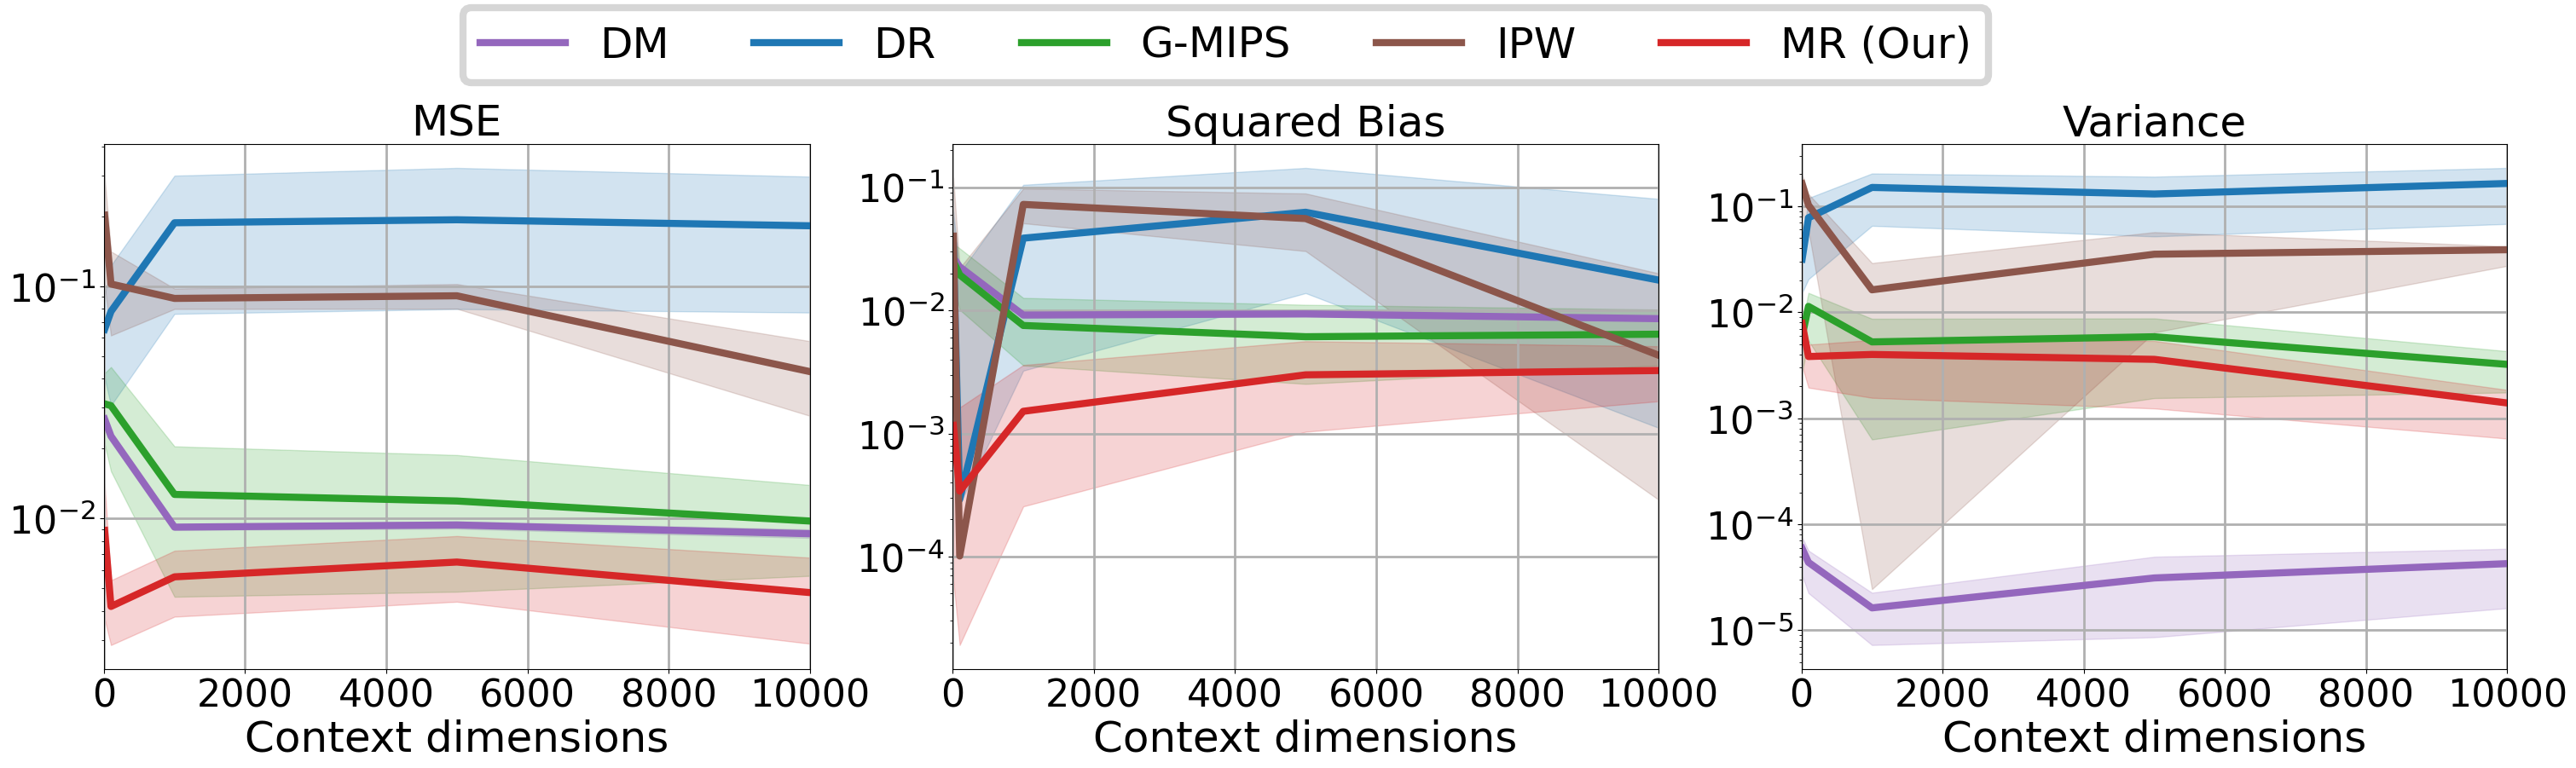
\includegraphics[width=0.75\textwidth]{figures/mr/ope_vs_dimc_nac_100_alphatar_0_8_neval_100_ntrain_100000.png}
%          \caption{Results with varying context dimensions $d$ for $n_{a}=100$, $n = 100$, $\alpha^\ast = 0.8$.}
%          \label{fig:mse-vs-d}
%      \end{subfigure}\\
%      \begin{subfigure}[b]{1\textwidth}
%          \centering
%          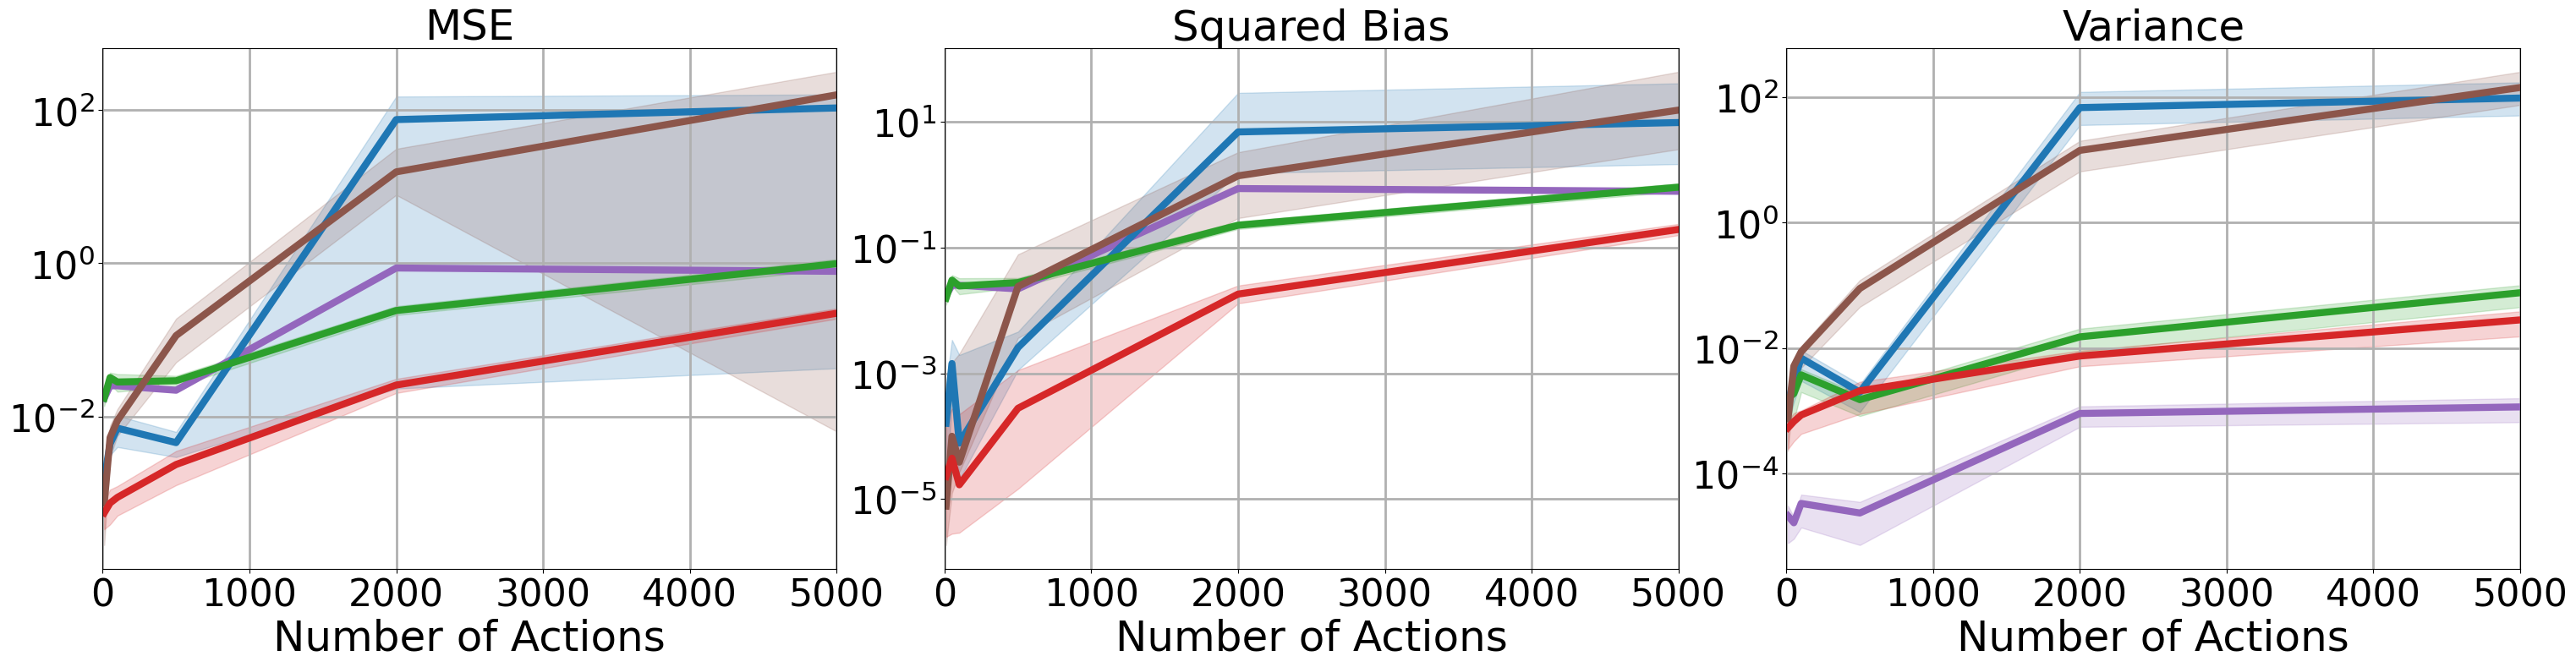
\includegraphics[width=0.75\textwidth]{figures/mr/ope_vs_nac_dimc_100_alphatar_0_2_neval_100_ntrain_100000.png}
%          \caption{Results with varying number of actions $n_{a}$ for $d=100$, $n = 100$, $\alpha^\ast = 0.2$.}
%          \label{fig:mse-vs-nac}
%      \end{subfigure}
%         \caption{Results with increasing $d$ and $n_a$.}
%         \label{fig:syn_results2}
% \end{figure}
% \paragraph{Varying $d$}
% Figure \ref{fig:mse-vs-d} plots how the results for different estimators changes as the context dimensions $d$ increases. While the results for the different baselines do not change significantly with increasing $d$, overall the MSE of MR estimator is smaller than that of other baselines.


% \paragraph{Varying $n_a$}
% Figure \ref{fig:mse-vs-nac} plots how the performance of different estimators changes as the number of actions $n_a$ increases. 
% It can be seen that the MSE and variance of IPW and DR estimators explodes when $n_a \geq 2000$. This happens because the variance of the policy ratios $\rho(a, x)$ is very large for large action spaces. In contrast, the MSE and variances of MR estimator remains relatively small even when $n_a$ is large. This shows that MR remains significantly robust in large action spaces. 

% Again, the MSE of MR estimator remains significantly smaller than the baselines with increasing values of $n_a$.
% \faaiz{think about plotting results versus the variance of policy ratios $\rho(x, a)$.}

\section{Discussion}
% \begin{itemize}
%     \item In this paper, we present marginal ratio estimator (MR) for off-policy evaluation which only considers the shift in the marginal distribution of the rewards resulting from the policy shift.
%     \item We show, theoretically and empirically, that the proposed method achieves better variance and MSE than the current SOTA methods, and is more data efficient overall.
%     \item We also show that our proposal can be used in the setting of causal inference, and provides more accurate results than the most commonly used methods.
% \end{itemize}

In this paper, we proposed an OPE method for contextual bandits called marginal ratio (MR) estimator, which considers only the shift in the marginal distribution of the outcomes resulting from the policy shift. Our theoretical and empirical analysis showed that MR achieves better variance and MSE compared to the current state-of-the-art methods and is more data efficient overall. Additionally, we demonstrated that MR applied to ATE estimation provides more accurate results than most commonly used methods. Next, we discuss limitations of our methodology and possible avenues for future work.

\myparagraph{Limitations}
The MR estimator requires the additional step of estimating $\hat{w}(y)$ which may introduce an additional source of bias in the value estimation. However, $\hat{w}(y)$ can be estimated by solving a simple 1d regression problem, and as we show empirically in Appendix \ref{app:experiments}, MR achieves the smallest bias among all baselines considered in most cases. Most notably, our ablation study in Appendix \ref{subsec:mips-empirical} shows that even when the training data is reasonably small, MR outperforms the baselines considered. 
% When the behaviour policy $\beh$ is unknown, MR estimator requires the splitting of training data to first estimate $\beh$ and subsequently to use this to estimate marginal weights $w(y)$. This data splitting can be costly in low-data settings, where we do not have access to large training datasets. However, as we empirically show in Appendix \ref{subsec:additional-experiments}, even when the training data is small, MR outperforms the baselines.  


\myparagraph{Future work}
The MR estimator can also be applied to policy optimisation problems, where the data collected using an `old' policy is used to learn a new policy. This approach has been used in Proximal Policy Optimisation (PPO) \citep{schulman2017proximal} for example, which has gained immense popularity and has been applied to reinforcement learning with human feedback (RLHF) \citep{lambert2022illustrating}. We believe that the MR estimator applied to these methodologies could lead to improvements in the stability and convergence of these optimisation schemes, given its favourable variance properties.


        \section*{Acknowledgements}
We would like to thank Jake Fawkes, Siu Lun Chau, Shahine Bouabid and Robert Hu for their useful feedback. 
We also appreciate the insights and constructive criticisms provided by the anonymous reviewers.
MFT acknowledges his PhD funding from Google DeepMind.

    }
    { % If compilePapers is false, this block will be executed
    }

% % \section{Motivation}

\begin{abstract}
% Off-Policy Evaluation (OPE) in contextual bandits enables assessing new policies using existing data without experimentation. Current OPE methods, such as Inverse Probability Weighting (IPW) and Doubly Robust (DR) estimators, suffer from high variance, particularly when there is low overlap between target and behavior policies or large action and context spaces. In this paper, we propose a novel OPE estimator, the Marginal Ratio (MR) estimator, which focuses on the shift in the marginal distribution of outcomes $Y$ rather than the policies themselves. We theoretically show that the MR estimator is more efficient and has lower variance compared to conventional methods like IPW and DR. Furthermore, we establish a connection between the MR estimator and the state-of-the-art Marginalized Inverse Propensity Score (MIPS) estimator, demonstrating that MR achieves the lowest variance among a generalized family of MIPS estimators. We also demonstrate the applicability of the MR estimator in causal inference settings for estimating Average Treatment Effects (ATE), where it outperforms state-of-the-art methods. Our contributions are supported by theoretical analyses and experiments on synthetic and real-world datasets, highlighting the improved performance of the MR estimator.

% Off-Policy Evaluation (OPE) in contextual bandits is crucial for assessing new policies using existing data without costly experimentation. However, current OPE methods, such as Inverse Probability Weighting (IPW) and Doubly Robust (DR) estimators, suffer from high variance, particularly in cases of low overlap between target and behavior policies or large action and context spaces. In this paper, we introduce a new OPE estimator for contextual bandits, the Marginal Ratio (MR) estimator, which focuses on the shift in the marginal distribution of outcomes $Y$ instead of the policies themselves. Through rigorous theoretical analysis, we demonstrate the benefits of MR estimator compared to conventional methods like IPW and DR in terms of variance reduction. Additionally, we establish a connection between our MR estimator and the state-of-the-art Marginalized Inverse Propensity Score (MIPS) estimator, proving that MR attains the lowest variance among a generalized family of MIPS estimators. We further showcase the versatility of the MR estimator in causal inference settings, where it surpasses current state-of-the-art methods in estimating Average Treatment Effects (ATE). Our extensive experiments on synthetic and real-world datasets corroborate our theoretical findings, emphasizing the superiority of the MR estimator in performance and practical applicability, making it a compelling choice for OPE in contextual bandits.


Off-Policy Evaluation (OPE) in contextual bandits is crucial for assessing new policies using existing data without costly experimentation. However, current OPE methods, such as Inverse Probability Weighting (IPW) and Doubly Robust (DR) estimators, suffer from high variance, particularly in cases of low overlap between target and behavior policies or large action and context spaces. In this paper, we introduce a new OPE estimator for contextual bandits, the Marginal Ratio (MR) estimator, which focuses on the shift in the marginal distribution of outcomes $Y$ instead of the policies themselves. Through rigorous theoretical analysis, we demonstrate the benefits of the MR estimator compared to conventional methods like IPW and DR in terms of variance reduction. Additionally, we establish a connection between the MR estimator and the state-of-the-art Marginalized Inverse Propensity Score (MIPS) estimator, proving that MR achieves lower variance among a generalized family of MIPS estimators. We further illustrate the utility of the MR estimator in causal inference settings, where it exhibits enhanced performance in estimating Average Treatment Effects (ATE). Our experiments on synthetic and real-world datasets corroborate our theoretical findings and highlight the practical advantages of the MR estimator in OPE for contextual bandits. 
\end{abstract}
% \emph{Off-Policy Evaluation (OPE)} evaluates the performance of a new target policy which has not been deployed, only using the available observational data. 
% Various OPE methods have been proposed in the literature \citep{thomas2016data,saito2021evaluating,saito2022off,wang2017optimal}. However, these methods often suffer from high variance, leading to unreliable estimates when the data size is not large. Many methods have thus been proposed to alleviate this problem using methods such as Double robust methods \citep{dudik2014doubly}, however, the variance in these estimators can still increase as the variance of contexts or actions increases. In this paper, we propose \emph{marginal ratio (MR)} estimator, an alternative method of off-policy evaluation which does not depend on the context/action variance, and only considers the shift in distribution of outcomes as a result of the policy shift. We prove that our proposed OPE estimator has lower variance compared to the most commonly used OPE estimator, the Inverse Probability Weighting (IPW) estimator.
\section{Introduction} 
% \begin{itemize}
%     \item In contextual bandits the goal is to take an action A based on some contextual information X to then maximize the outcome Y.
%     \item This setup is common in many real-world settings such as healthcare, personalized recommendation systems, and online advertising, etc \citep{li2010contextual, bastani2019online, xu2020contextual}, where the goal is to take actions i.e. taking a drug or recommending an item which subsequently leads to a desirable outcome such as the patients health or click in recommendations.
%     \item However a question arises when we want to change and update the policy. Hence, in the recent years much of research has been spent on evaluating how a new policy will do based on the collected data up to now. In particular, this is also known as the field of off-policy evaluation.
% \end{itemize}
% \begin{wrapfigure}{r}{0.5\textwidth}
%     \centering
%     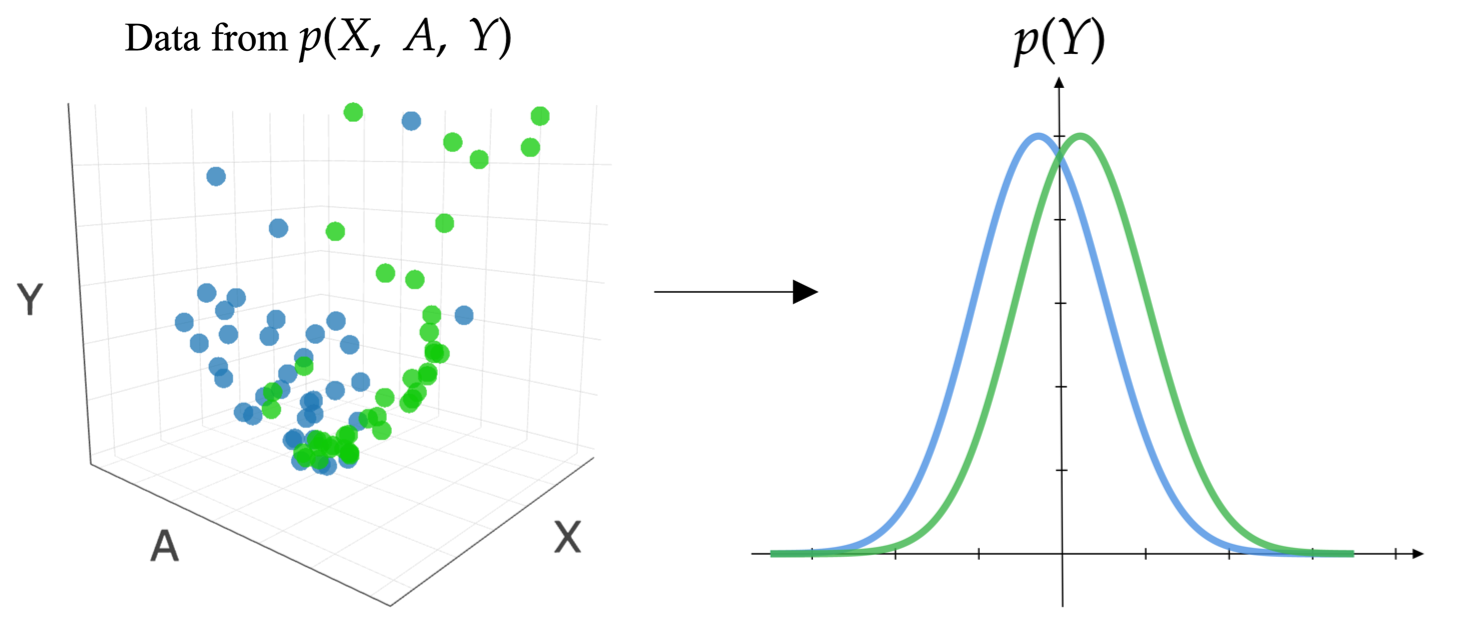
\includegraphics[width=0.5\textwidth]{figures/mr/main_pic.png}
%     \caption{Caption}
%     % \vspace{-1cm}
%     \label{fig:my_label}
% \end{wrapfigure}
In contextual bandits, the objective is to select an action $A$, guided by contextual information $X$, to maximize the resulting outcome $Y$. This paradigm is prevalent in many real-world applications such as healthcare, personalized recommendation systems, or online advertising \citep{li2010contextual, bastani2019online, xu2020contextual}. The objective is to perform actions, such as prescribing medication or recommending items, which lead to desired outcomes like improved patient health or higher click-through rates. Nonetheless, updating the policy presents challenges, as na\"ively implementing a new, untested policy may raise ethical or financial concerns. For instance, prescribing a drug based on a new policy poses risks, as it may result in unexpected side effects. As a result, recent research \citep{swaminathan2015counterfactual, wang2017optimal, farajtabar2018more, su2019continuous, metelli2021subgaussian, liu2019triply, sugiyama2012machine, swaminathan2017off} has concentrated on evaluating the performance of new policies (target policy) using only existing data that was generated using the current policy (behaviour policy). This problem is known as Off-Policy Evaluation (OPE).


Current OPE methods in contextual bandits, such as the Inverse Probability Weighting (IPW) \citep{horvitz1952generalization} and Doubly Robust (DR) \citep{dudik2014doubly} estimators primarily account for the policy shift by re-weighting the data using the ratio of the target and behaviour polices to estimate the target policy value. This can be problematic as it may lead to high variance in the estimators in cases of substantial policy shifts. The issue is further exacerbated in situations with large action or context spaces \citep{saito2022off}, since in these cases the estimation of policy ratios is even more difficult leading to extreme bias and variance.
% The problem is worsened in the policy ratios are even harder to estimate in these cases. 
% even when the distribution of outcome $Y$ changes minimally.
% \jef{Nonetheless, these methods possess a fundamental limitation, as they explicitly account for the shift between behavior and target policies when estimating the expected target policy value.} 
% As a result, the estimators may demonstrate high variance in cases of substantial policy shifts, even when the outcome distribution in $Y$ changes minimally. 
% This high variance in estimators can lead to unreliable and potentially vacuous outputs. 

% In light of these concerns, since our goal is to estimate the expected outcome $Y$ under a new target policy, we show that directly considering the shift in the marginal distribution of outcomes $Y$ rather than the shift in the policies leads to a more efficient estimator.

% Given our goal of estimating the expected outcome $Y$ under a new target policy, we show that directly considering the shift in the marginal distribution of outcomes $Y$

In this work we show that this problem of high variance in OPE can be alleviated by using methods which directly consider the shift in the marginal distribution of the outcome $Y$ resulting from the policy shift, instead of considering the policy shift itself (as in IPW and DR). To this end, we propose a new OPE estimator for contextual bandits called the Marginal Ratio (MR) estimator, which weights the data directly based on the shift in the marginal distribution of outcomes $Y$ and consequently is much more robust to increasing sizes of action and context spaces than existing methods like IPW or DR. 
% Since our goal is to estimate the expected outcome $Y$ under a new target policy, we show that 
% the problem of high variance that arises as a result of weighting the data using policy ratios can be circumvented by instead weighting the data directly based on the shift in the marginal distribution of outcomes $Y$.
% the problem of high variance can be alleviated by weighting the data directly based on the shift in the marginal distribution of outcomes $Y$ resulting from the policy shift rather than the policy ratios (as in IPW or DR).
% directly considering the shift in the marginal distribution of outcomes $Y$ rather than 
% To this end, we propose a new OPE estimator for contextual bandits called the Marginal Ratio (MR) estimator, which directly takes into account the shift in the marginal distribution of the outcome and consequently is much more robust to increasing sizes of action and context spaces than existing methods like IPW or DR. 
Our extensive theoretical analyses show that MR enjoys better variance properties than the existing methods making it highly attractive for a variety of applications in addition to OPE. One such application is the estimation of Average Treatment Effect (ATE) in causal inference, for which we show that MR provides greater sample efficiency than the most commonly used methods.

Our contributions in this paper are as follows:
% and can also be used in domains like causal inference for the estimation of Average Treatment Effect (ATE) where it leads to desirable properties such as increased sample efficiency 
% Additionally, we theoretically show that MR enjoys better variance properties than
% achieves significant variance reduction compared to 
% conventional methods (like IPW or DR) and consequently is much more robust to increasing sizes of action and context spaces.
% Additionally, we also show that the MR estimator can be applied in causal inference for the estimation of Average Treatment Effect (ATE). We demonstrate theoretically and empirically that the MR estimator is more sample efficient than existing methods. Our contributions in this paper are:



% by weighting the samples based on how relevant the observed \emph{outcome} is to the target outcome distribution.

% Our proposed method aims to offer a more robust solution, mitigating the adverse effects of high variance and providing a reliable alternative to existing OPE techniques. 
% At a high level, instead of weighting the samples based on the policy shift as in IPW, the MR estimator weights the samples based on how relevant the observed \emph{outcome} is to target outcome distribution.

% Current OPE methods in contextual bandits, such as the inverse propensity weighting (IPW) \citep{horvitz1952generalization} and doubly robust (DR) \citep{dudik2014doubly} estimators, have gained considerable popularity in practice due to their ability to estimate the expected value of a modified policy. However, these methods have an inherent limitation, as they explicitly consider the shift between behavior and target policies when estimating the target policy value. Consequently, the estimators can exhibit high variance when there is a significant policy shift, even if the change in the outcome distribution is minimal. This issue can be especially pronounced in scenarios with large action or context spaces \citep{saito2022off}.



% Contextual bandits are a prevalent framework \jef{need to rewrite this banditS are A framework doesnt sound right} used in several real-world applications, including healthcare, personalized recommendation systems, and online advertising \citep{li2010contextual, bastani2019online, xu2020contextual}\faaiz{more refs}. In this setup, an agent takes actions $A$ based on contextual information $X$, and receives outcomes $Y$ accordingly. In such settings \jef{Two times start with IN}, evaluating the effectiveness of a new policy without actually deploying it is often desirable \jef{Due to potential financial or ethical reasons + refs}. \jef{Would start this with: Hence, in recent years, researchers have ... }Off-policy evaluation (OPE) is a popular approach that estimates the expected value of a \jef{a or the?} random variable $Y$ under a target policy $\tar$, without deploying the target policy \citep{swaminathan2015counterfactual, wang2017optimal, farajtabar2018more, su2019continuous, metelli2021subgaussian, liu2019triply, sugiyama2012machine, swaminathan2017off}.

% Current OPE methods in contextual bandits focus on the shift in the joint distribution of the context, action, and outcome when estimating the expected value \jef{this sentence is coming out of nowhere}. These methods, such as the inverse propensity weighting (IPW) \citep{horvitz1952generalization} and doubly robust (DR) \citep{dudik2014doubly} estimators, have been highly popular in practice \jef{This should come first}. However, they have a fundamental limitation: they explicitly take the shift between behaviour and target policies into account when estimating target policy value. \jef{we might want to be more vague here in case people do not understand the problem of the ratios, or we have to be way more concrete}


% \jef{I will use AB review from now on :) }


% do not only take the shift in the distribution of the outcome into account, but also the shift in the distribution of the actions. 
% As a result, the estimators can have high variance when the policy shift is large, even if the shift in the outcome distribution is small. This issue can be particularly pronounced in large action or context spaces \citep{saito2022off}.

% To address this limitation, we propose a new OPE estimator for contextual bandits that only takes into account the shift in the marginal distribution of the outcome as a result of the policy shift. Our estimator, called Marginal Ratio (MR) estimator, utilizes the available logged data more efficiently and leads to lower variance than the current state-of-the-art methods. At a high level, instead of weighting the samples based on the policy shift as in IPW, the MR estimator weights the samples based on how relevant the observed \emph{outcome} is to target outcome distribution.
% assigns high weights to the samples where the observed outcomes are most relevant to the target outcome distribution.  

\begin{itemize}
    \item Firstly, we introduce MR, an OPE estimator for contextual bandits, that focuses on the shift in the marginal distribution of $Y$ rather than the joint distribution of $(X, A, Y)$. 
    \flag{We show that MR has favourable theoretical properties compared to existing methods like IPW and DR. Our analysis also encompasses theory on the approximation errors of our estimator. 
    % that MR achieves lower variance than conventional OPE methods like IPW.
    }
    % We provide extensive theoretical comparisons to show  the variance reduction properties of MR compared to existing approaches such as IPW and DR.
    % at MR achieves lower variance than IPW and DR estimators. 
    
    \item Secondly, we explicitly lay out the connection between MR and  Marginalized Inverse Propensity Score (MIPS) \cite{saito2022off}, a recent state-of-the-art contextual bandits OPE method, and prove that MR attains lowest variance among a generalized family of MIPS estimators. 
    \item Thirdly, we show that the MR estimator can be applied in the setting of causal inference to estimate average treatment effects (ATE), and theoretically prove that the resulting estimator is more data-efficient with higher accuracy and lower variance than commonly used methods. 
    \item Finally, we verify all our theoretical analyses through a variety of experiments on synthetic and real-world datasets and empirically demonstrate that the MR estimator achieves better overall performance compared to current state-of-the-art methods. 
\end{itemize}
% Firstly, we introduce MR, an OPE estimator for contextual bandits that focuses on the shift in the marginal distribution of $Y$ rather than the joint distribution of $(X, A, Y)$. Specifically, we provide extensive theoretical comparisons which show that MR achieves lower variance than classical importance-weighted estimators like IPW and DR. Our analysis also encompasses theory on the estimation errors of our estimator. Secondly, we explicitly layout the connection between MR and  Marginalized Inverse Propensity Score (MIPS) \cite{saito2022off}, a recent state-of-the-art contextual bandits OPE method, and demonstrate that MR attains lowest variance among a generalized family of MIPS estimators. Thirdly, we show that the MR estimator can be applied in the setting of causal inference to estimate average treatment effects (ATE), and theoretically prove that the resulting estimator is more data-efficient with higher accuracy and lower variance than commonly used methods. Finally, we verify all our theoretical analyses through a variety of experiments on synthetic and real-world datasets and empirically demonstrate that the MR estimator achieves better overall performance compared to current state-of-the-art methods. 

%  Our contributions in this paper are fourfold.
% \begin{enumerate}[label=\roman*.]
%     \item We introduce MR, an OPE estimator for contextual bandits that focuses on the shift in the marginal distribution of $Y$ rather than the joint distribution of $(X, A, Y)$. Specifically, we provide extensive theoretical comparisons 
%     which show that MR achieves lower variance than classical importance-weighted estimators like IPW and DR.
%     Our analysis also encompasses theory on the estimation errors of our estimator.
%     % In addition, we provide convergence rates for our estimator.
%     % Moreover, we show that MR is likely to achieve lower variance than the DR method when the dimensions of context $X$ are large.
%     % \item We provide theoretical results comparing the performance of MR against the most commonly used OPE estimators for contextual bandits. We prove that the variance of our estimator is lower than that of the classical importance-weighted estimator (IPW). Additionally, we contrast MR against the recently proposed MIPS estimator \citep{saito2022off} and show that MR achieves the optimal variance over the class of all MIPS estimators.
%     \item We explicitly layout the connection between MR and  Marginalized Inverse Propensity Score (MIPS) \cite{saito2022off}, a current state-of-the-art contextual bandits OPE method, and demonstrate that MR attains lowest variance among a generalized family of MIPS estimators.
%     \item We show that the MR estimator can be applied in the setting of causal inference to estimate average treatment effects (ATE), and theoretically prove that the resulting estimator is more data-efficient with higher accuracy and lower variance than commonly used methods.
%     \item We verify all our theoretical analyses through a variety of experiments on synthetic and real-world datasets and empirically demonstrate that the MR estimator achieves better overall performance compared to current state-of-the-art methods.
%     % \item We show that the MR estimator can be applied in the setting of causal inference to estimate average treatment effects (ATE), and leads to a more data-efficient estimator with higher accuracy and lower variance than the most commonly used methods.
%     % \item We verify our analysis on a variety of experiments on synthetic datasets as well as real-world datasets. We empirically show that MR achieves better performance overall compared to the current state-of-the-art methods.
% \end{enumerate}

% First, we propose a new off-policy evaluation (OPE) estimator, called MR, which only takes into account the shift in the marginal distribution of $Y$ instead of the joint distribution of $(X, A, Y)$. Second, we provide theoretical results comparing the performance of MR against the most commonly used OPE estimators for contextual bandits. We prove that the variance of our estimator is lower than that of the classical importance-weighted estimator (IPW). Additionally, we contrast MR against the recently proposed MIPS estimator \citep{saito2022off} and show that MR achieves the optimal variance over the class of all MIPS estimators. Third, we show that the MR estimator can be applied in the setting of causal inference to estimate average treatment effects (ATE), and leads to a more data-efficient estimator with high accuracy and low variance than the most commonly used methods.  Finally, we verify our analysis on a variety of experiments on synthetic datasets as well as real-world datasets. We empirically show that MR achieves better performance overall compared to the current state-of-the-art methods. 
% Our proposed method, MR, can therefore be seen as a significant contribution to the field of off-policy evaluation for contextual bandits.

% Specifically, we provide theoretical results showing that the variance of MR is lower than those of the classical IPW estimator, and the recently proposed MIPS estimator \citep{saito2022off}. We also show that MR achieves the optimal variance over the class of all MIPS estimators.

% In addition to the theoretical analysis, we evaluate the performance of MR on both synthetic and real-world classification datasets. Our experiments demonstrate that MR achieves better performance overall compared to the existing methods. Overall, our proposed MR estimator presents a significant contribution to the OPE problem in contextual bandits, providing a more efficient and accurate way to estimate the expected value of a random variable under a target policy


\section{Background}
\subsection{Setup and Notation} \label{sec:setup_notation}
We consider the standard contextual bandit setting. Let $X\in\Xspace$ be a context vector (e.g., user features), $A\in \Aspace$ denote an action (e.g., recommended website to the user), and $Y\in \Yspace$ denote a scalar reward or outcome (e.g., whether the user clicks on the website). The outcome and context are sampled from unknown probability distributions $p(y\mid x, a)$ and $p(x)$ respectively. Let $\D\coloneqq \{(x_i, a_i, y_i)\}_{i=1}^n$ be a historically logged dataset with $n$ observations, generated by a (possibly unknown) \emph{behaviour policy} $\beh(a\mid x)$.
Specifically, $\D$ consists of i.i.d. samples from the joint density under\textit{ behaviour policy},
\begin{align}
    \pbeh(x, a, y) \coloneqq p(y\mid x, a)\, \textcolor{blue}{\beh(a\mid x)}\,p(x). \label{eq:behav-joint-factorisation}
\end{align}
We denote the joint density of $(X, A, Y)$ under the \textit{target policy} as
\begin{align}
    \ptar(x, a, y) \coloneqq p(y\mid x, a)\, \textcolor{red}{\tar(a\mid x)}\,p(x). \label{eq:tar-joint-factorisation}
\end{align}

Moreover, we use $\pbeh(y)$ to denote the marginal density of $Y$ under the behaviour policy, 
\begin{align*}
    \pbeh(y) &= \int_{\Aspace \times \Xspace} \pbeh(x, a, y)\, \mathrm{d}a \, \mathrm{d}x,
\end{align*}
and likewise for the target policy $\tar$. Similarly, we use $\Ebeh$ and $\Etar$ to denote the expectations under the joint densities $\pbeh(x, a, y)$ and $\ptar(x, a, y)$ respectively.


\myparagraph{Off-policy evaluation (OPE)}
The main objective of OPE is to estimate the expectation of the outcome $Y$ under a given target policy $\tar$, i.e., $\Etar [Y]$, using only the logged data $\D$.
% \[
% \Etar [Y] \coloneqq \E_{(X, A, Y) \sim \ptar}[Y].
% \]


% \paragraph{Notation}
% We use $\pbeh(x, a, y)$ to denote the joint density of $(X, A, Y)$ under the behaviour policy, and $\ptar(x, a, y)$ to denote the joint density under target policy. The joint densities, whose factorisation only differs in the policies, can be written as follows:
% \begin{align}\label{eq:pxay}
%     \pbeh(x, a, y) &= p(y\mid x, a)\, \textcolor{blue}{\beh(a\mid x)}\,p(x), \\
%     \ptar(x, a, y) &= p(y\mid x, a)\, \textcolor{red}{\tar(a\mid x)}\,p(x).
% \end{align}
% The historical logged data $\D$ comprises i.i.d. realisations from the joint density $\pbeh(x, a, y)$.
% Moreover, we use $\pbeh(y)$ to denote the marginal density of $Y$ under the behaviour policy, 
% \begin{align*}
%     \pbeh(y) &= \int_{\Aspace, \Xspace} \pbeh(x, a, y)\, \mathrm{d}a \, \mathrm{d}x,
% \end{align*}
% and likewise for the target policy $\tar$. Similarly, we use $\Ebeh$ and $\Etar$ to denote the expectations under the joint densities $\pbeh(x, a, y)$ and $\ptar(x, a, y)$ respectively.

% \paragraph{Off-policy evaluation}
% Given logged data $\D$, our goal is to estimate the following expectation
% \[
% \Etar [Y] \coloneqq \E_{(X, A, Y) \sim \ptar}[Y].
% \]

Throughout this work, we assume that the support of the target policy $\tar$ is included in the support of the behaviour policy $\beh$. This is to ensure that importance sampling yields unbiased off-policy estimators, and is satisfied for exploratory behaviour policies such as the $\epsilon$-greedy policies. 
\begin{assumption}[Support]
    For any $x \in \Xspace, a \in \Aspace$,  $\tar(a\mid x) >0 \implies \beh(a\mid x) >0$. 
\end{assumption}
% This is a mild assumption which
 

\subsection{Existing off-policy evaluation methodologies}
Next, we will present some of the most commonly used OPE estimators before outlining the limitations of these methodologies. This motivates our proposal of an alternative OPE estimator. 

The value of the target policy can be expressed as the expectation of outcome $Y$ under the target data distribution $\ptar(x, a, y)$.
% The policy value of target policy $\tar$ can be written as:
% \[
% \Etar[Y] = \int_{\Xspace, \Aspace, \Yspace} y\, \ptar(x, a, y) \, \mathrm{d}x \, \mathrm{d}a \, \mathrm{d}y.
% \]
However in most cases, we do not have access to samples from this target distribution and hence we have to resort to importance sampling methods.
\paragraph{Inverse Probability Weighting (IPW) estimator}
One way to compute the target policy value, $\Etar[Y]$, when only given data generated from $\pbeh(x, a, y)$ is to rewrite the policy value as follows:
% _{\Xspace, \Aspace, \Yspace}
\begin{small}
\begin{align*}
    \Etarred[Y] =
    \int y \, \ptar(x, a, y) \,\mathrm{d}y \, \mathrm{d}a\, \mathrm{d}x   =
    \int y \, \underbrace{\frac{\ptar(x, a, y)}{\pbeh(x, a, y)}}_{\rho(a,x)}\, \pbeh(x, a, y) \,\mathrm{d}y \, \mathrm{d}a\, \mathrm{d}x =
    % \Ebehblue\left[Y\,\frac{\ptar(X, A, Y)}{\pbeh(X, A, Y)} \right] = 
    \Ebehblue\left[Y\,\rho(A, X)\right],
\end{align*}
\end{small} 
where 
$
\rho(a, x) \coloneqq \frac{\ptar(x, a, y)}{\pbeh(x, a, y)} = \frac{\tar(a|x)}{\beh(a|x)}
$, given the factorizations in Eqns. \eqref{eq:behav-joint-factorisation} and \eqref{eq:tar-joint-factorisation}.
This leads to the commonly used \emph{Inverse Probability Weighting (IPW)} \citep{horvitz1952generalization} estimator:
\[
\thetaipw \coloneqq \frac{1}{n}\sum_{i=1}^n \rho(a_i, x_i)\,y_i.
\]
When the behaviour policy is known, IPW is an unbiased and consistent estimator. However, it can suffer from high variance, especially as the overlap between the behaviour and target policies decreases. 

\myparagraph{Doubly Robust (DR) estimator} 
To alleviate the high variance of IPW, \cite{dudik2014doubly} proposed a \emph{Doubly Robust (DR)} estimator for OPE. 
DR uses an estimate of the conditional mean $\hat{\mu}(a, x) \approx\E[Y\mid X=x, A=a]$ (\emph{outcome model}), as a control variate to decrease the variance of IPW. It is also doubly robust in that it yields accurate value estimates if either the importance weights $\rho(a, x)$ or the outcome model $\hat{\mu}(a, x)$ is well estimated \citep{dudik2014doubly, jiang2016doubly}. 
The DR estimator for $\Etar[Y]$ can be written as follows:
\[
\thetadr = \frac{1}{n} \sum_{i=1}^n \rho(a_i, x_i)\,(y_i - \hat{\mu}(a_i, x_i)) + \hat{\eta}(\tar),
% \vspace{-0.7mm}
\]
where
$
\hat{\eta}(\tar) = \frac{1}{n} \sum_{i=1}^n \sum_{a'\in \Aspace} \hat{\mu}(a', x_i) \tar(a'\mid x_i) \approx \E_{\tar}[\hat{\mu}(A, X)]$. Here, $\hat{\eta}(\tar)$ is referred to as the Direct Method (DM) as it uses $\hat{\mu}(a, x)$ directly to estimate target policy value. 

\subsection{Limitation of existing methodologies} 
To estimate the value of the target policy $\tar$, the existing methodologies consider the shift in the joint distribution of $(X, A, Y)$  as a result of the policy shift (by weighting samples by policy ratios). As we show in Section \ref{subsec:comparison}, considering the joint shift can lead to inefficient policy evaluation and high variance especially as the policy shift increases \citep{li2018addressing}.
Since our goal is to estimate $\Etar[Y]$, we will show in the next section that considering only the shift in the marginal distribution of the outcomes $Y$ from $\pbeh(Y)$ to $\ptar(Y)$, leads to a more efficient OPE methodology compared to existing approaches.

To better comprehend why only considering the shift in the marginal distribution is advantageous, let us examine an extreme example where we assume that $Y \indep A \mid X$, i.e., the outcome $Y$ for a user $X$ is independent of the action $A$ taken. In this specific instance, $\Etar[Y] = \Ebeh[Y] \approx 1/n\sum_{i=1}^n y_i,$ indicating that an unweighted empirical mean serves as a suitable unbiased estimator of $\Etar[Y]$. However, IPW and DR estimators use policy ratios $\rho(a, x)  = \frac{\tar(a \mid x)}{\beh(a \mid x)}$ as importance weights. In case of large policy shifts, these ratios may vary significantly, leading to high variance in IPW and DR.

In this particular example, the shift in policies is inconsequential as it does not impact the distribution of outcomes $Y$. Hence, IPW and DR estimators introduce additional variance due to the policy ratios when they are not actually required. This limitation is not exclusive to this special case; in general, methodologies like IPW and DR exhibit high variance when there is low overlap between target and behavior policies \citep{li2018addressing} even if the resulting shift in marginals of the outcome $Y$ is not significant.
% This limitation is not exclusive to this special case; in general, methodologies like IPW and DR that use policy ratios as importance weights exhibit high variance when there is low overlap between target and behavior policies \citep{li2018addressing} or when the action and/or context spaces are large \citep{saito2022off}.

Therefore, we propose the \emph{Marginal Ratio (MR)} OPE estimator for contextual bandits in the subsequent section, which circumvents these issues by focusing on the shift in the marginal distribution of the outcomes $Y$. Additionally, we provide extensive theoretical insights on the comparison of MR to existing state-of-the-art methods, such as IPW and DR.

% To estimate the value of the target policy $\tar$, the existing methodologies consider the shift in the joint distribution of $(X, A, Y)$ as a result of the policy shift. As we show in Section \ref{subsec:comparison}, considering the joint shift can lead to inefficient policy evaluation and high variance especially as the policy shift increases \citep{li2018addressing}.
% Since our goal is to estimate $\Etar[Y]$, we will show in the next section that considering only the shift in the marginal distribution of the outcomes $Y$ from $\pbeh(Y)$ to $\ptar(Y)$, leads to a more efficient OPE methodology compared to existing approaches.

% To gain a better intuitive understanding why only considering the shift in the marginal distribution, let us take this extreme example, where we assume that $Y \indep A \mid X$, i.e. the outcome $Y$ of a user $X$ does not depend on the action taken. In this special example, $\Etar[Y] = \Ebeh[Y] \approx 1/n\sum_{i=1}^n y_i,$ and therefore, an unweighted empirical mean should be a good unbiased estimator of $\Etar[Y]$. However, the IPW and DR estimators use the policy ratios as importance weights since $\ptar(x, a, y)/\pbeh(x, a, y) = \tar(a \mid x)/\beh(a \mid x)$, and hence yield a higher variance estimator. 

% In this specific example, the shift in policies is meaningless as it has no effect on the distribution of outcomes $Y$, and therefore, the IPW and DR estimators incur extra variance due to the importance ratios when they are in fact not needed. This limitation is not restricted to this special case and in general, methodologies like IPW and DR which use policy ratios as importance weights will have high variance whenever there is low overlap between target and behaviour policies \citep{li2018addressing} or whenever the action and/or context spaces are large \citep{saito2022off}.

% Hence, we propose \emph{Marginal Ratio (MR)} OPE estimator for contextual bandits in the next section, which avoids these problems by only considering the shift in the marginal distribution of the outcomes $Y$. In addition, using the MR estimator, we are able to gain novel theoretical insights compared to existing SOTA methods such as IPW and DR methods in terms of variance reduction.






% Since our goal is to estimate $\Etar[Y]$, it suffices to consider only the shift in the marginal distribution of the outcomes $Y$ from $\pbeh(y)$ to $\ptar(y)$. Instead, methodologies like IPW and DR consider the shift in the joint distribution of $(X, A, Y)$ which can lead to inefficient policy evaluation and high variance especially as the policy shift increases \citep{li2018addressing}.
% In the next section, we propose \emph{Marginal Ratio (MR)} OPE estimator which circumvents the limitations outlined above, by only considering the shift in the marginal distribution of the outcomes $Y$. 
% Similarly, we could also consider another example, where the action $a \in [-100, 100]$ is related to $Y$ through a simple function such as $Y=x$ for $a < 0$ and $Y=-x$ for $a > 0$. In this case, modelling the ratio of the policy which for ever action, would unnecessarily complicate as computation. \jef{to be completed}
% \jef{TODO} The following special case makes this idea more concrete. Assume that $Y \indep A \mid X$, i.e. the outcome $Y$ of a user $X$ does not depend on the action taken. In this case $\Etar[Y] = \Ebeh[Y] \approx 1/n\sum_{i=1}^n y_i,$ and therefore, an unweighted empirical mean should be a good unbiased estimator of $\Etar[Y]$. However, the IPW and DR estimators use the policy ratios as importance weights since $\ptar(x, a, y)/\pbeh(x, a, y) = \tar(a \mid x)/\beh(a \mid x)$, and hence yield a weighted estimator. \faaiz{to be fixed}

\section{Marginal Ratio (MR) estimator}
 
% \subsection{Marginal Ratio (MR) estimator}
% The main insight of our methodology is to weight the outcomes using the ratio of marginal density of the outcome $Y$, i.e.,
Our method's key insight involves weighting outcomes by the marginal density ratio of outcome $Y$:
\begin{align*}
\Etarred[Y] &= \int_{\Yspace} y \, \ptar(y)\, \mathrm{d}y = \int_\Yspace y\, \frac{\ptar(y)}{\pbeh(y)} \, \pbeh(y) \, \mathrm{d}y = \Ebehblue\left[Y\, w(Y) \right],
\end{align*}
where 
$
w(y) \coloneqq \frac{\ptar(y)}{\pbeh(y)}.
$
This leads to the Marginal Ratio OPE estimator:
\begin{align*}
    \thetamr \coloneqq \frac{1}{n}\sum_{i=1}^n w(y_i) \, y_i.
\end{align*}

In Section \ref{subsec:comparison} we prove that by only considering the shift in the marginal distribution of outcomes, the MR estimator achieves a lower variance than the standard OPE methods. In fact, this estimator does not depend on the shift between target and behaviour policies directly. Instead, it depends on the shift between the marginals $\pbeh(y)$ and $\ptar(y)$.
% Moreover, when the weights $w(y)$ are known exactly, the MR estimator is unbiased and consistent.
% \jef{I recon we can chuck this}
% \jef{Need to change and think as well} Recall that in our previous example with $Y \indep A\mid X$, any policy shift has no effect on the marginal outcome distribution and the weights $w(y)\equiv 1$ for any target and behaviour policies. Therefore $\thetamr = 1/n \sum_{i=1}^n y_i$, i.e., MR leads to an unweighted estimator which is unbiased and does not incur any extra variance arising from the importance weights $\tar(a\mid x)/\beh(a\mid x)$.
% Before we go on to prove the variance reduction, we first outline how to efficiently compute the weights $w(y)$ using the logged data $\D$.
% To start, let us outline an efficient way to estimate the weights $w(y)$ using the logged data $\D$, before moving on to prove the variance reduction.

\myparagraph{Estimation of $w(y)$} When the weights $w(y)$ are known exactly, the MR estimator is unbiased and consistent. However, in practice the weights $w(y)$ are often not known and must be estimated using the logged data $\D$. Here, we outline an efficient way to estimate $w(y)$ by first representing it as a conditional expectation, which can subsequently be expressed as the solution to a regression problem.
% \jef{Add references as mentioned by Arnaud}
% \begin{align}\label{eq:ratioidentity}
%     w(y)=\frac{\ptar(y)}{\pbeh(y)} =\int_{\Xspace, \Aspace} \frac{\ptar(x,a,y)}{\pbeh(x,a,y)}\,\pbeh(a, x|y)\,\mathrm{d}a\, \mathrm{d}x  
%     % &=\int_{\Xspace, \Aspace} \frac{\pi^{\ast}(a|x)}{\beh (a|x)}\,\pbeh(a, x|y)\,\mathrm{d}a \,\mathrm{d}x \nonumber\\
%     &= \Ebeh\Bigg[ \frac{\pi^{\ast}(A|X)}{\beh (A|X)} \Bigg| \,Y=y \Bigg]. 
% \end{align}
% \faaiz{make this a complete sentence}
\begin{lemma}\label{lemma:weights-est}
Let $w(y)=\frac{\ptar(y)}{\pbeh(y)}$ and $\rho(a, x) = \frac{\tar(a\mid x)}{\beh(a\mid x)}$, then $w(y) = \Ebeh\left[ \rho(A, X) \mid \,Y=y \right]$, and,
% \[
% w(y)= \Ebeh\left[ \rho(A, X) \mid \,Y=y \right], \quad \textup{and consequently,} \quad w = \arg\min_{f} \, \Ebeh \left[(\rho(A, X)-f(Y))^2\right]. 
% \]
% Additionally,
\begin{align}
 w = \arg\min_{f} \, \Ebeh \left[(\rho(A, X)-f(Y))^2\right]. \label{eq:weights-obj}
\end{align}
\end{lemma}
% \vspace{-2mm}
Lemma \ref{lemma:weights-est} allows us to approximate $w(y)$ using a parametric family $\{f_\phi: \mathbb{R}\rightarrow \mathbb{R} \mid \phi \in \Phi\}$ (e.g.\ neural networks) and defining $\hat{w}(y)\coloneqq f_{\phi^*}(y)$, where $\phi^*$ solves the regression problem in Eq. \eqref{eq:weights-obj}. 

% Hence, the weights $w(y)$ can be estimated by solving the regression problem in Eq. \eqref{eq:weights-obj}. 
% Similar techniques of estimating ratios of marginal densities have also been used in areas like likelihood-free inference \citep{brehmer2020mining}.
% Similar techniques have also been used in areas like likelihood-free inference \citep{brehmer2020mining} to estimate the ratio of marginal densities.

% \paragraph{Proof of Lemma \ref{prop:weights-est}}
% This follows directly from the identity \eqref{eq:ratioidentity}. 
% We prove it here for the sake of completeness.
% \begin{align}
%     &\Ebeh \Bigg[\frac{\pi^{\ast}(A|X)}{\beh (A|X)}-f(Y)\Bigg]^2 \nonumber \\
%     &= \mathbb{E}_{X,Y \sim P^{\beh}_{X,Y}} \Big[\E_{A \sim P^{\beh}_{A\mid X,Y}} \Big|\Big|\frac{\pi^{\ast}(A|X)}{\beh (A|X)}-f(X,Y)\Big|\Big|^2\Big] \nonumber \\
%     &= \mathbb{E}_{X,Y \sim P^{\beh}_{X,Y}} \Big[\textup{Var}_{A \sim P^{\beh}_{A\mid X,Y}}\Big[ \frac{\pi^{\ast}(A|X)}{\beh (A|X)} \Big] + \left(\E_{A \sim P^{\beh}_{A\mid X,Y}}\Big[ \frac{\pi^{\ast}(A|X)}{\beh (A|X)} \Big] - f(X,Y) \right)^2 \Big].
%      \label{eq:w-reg}
% \end{align}
% Where, \eqref{eq:w-reg} is minimized if $f(x, y) = \E_{A \sim P^{\beh}_{A\mid X=x,Y=y}}\Big[ \frac{\pi^{\ast}(A|x)}{\beh (A|x)} \Big] = w(x,y)$.

% \begin{align}
%     \theta^* \coloneqq \arg \min_{\theta} \Ebeh \Bigg(\frac{\pi^{\ast}(A|X)}{\beh (A|X)}-f_\theta(Y)\Bigg)^2 \label{eq:weights-loss}
% \end{align}

Note that MR can also be estimated alternatively by directly estimating $h(y) \coloneqq w(y)\,y$ 
% (instead of estimating the weights $w(y)$) 
using a similar regression technique as above and computing $\thetamr = 1/n \sum_{i=1}^n h(y_i)$. We include additional details along with empirical comparisons in Appendix \ref{sec:alt-estimation-method}. 
% In the next section, we provide theoretical analysis comparing the MR estimator with the existing methodologies. 

\begin{comment}
\subsubsection{Alternative estimation method}\label{sec:alt-estimation-method}
When estimating the MR estimator, we can alternatively estimate $h(y) \coloneqq y\,w(y)$ using 
\begin{align*}
    h = \arg\min_{f} \, \Ebeh \Bigg(Y\,\frac{\tar(A|X)}{\beh (A|X)}-f(Y)\Bigg)^2.
\end{align*}
Subsequently, the MR estimator can be written as:
\[
\thetamr = \frac{1}{n}\sum_{i=1}^n h(y_i).
\]
\paragraph{Remark}
These methods outline two different methodologies of estimating MR. In general, it is difficult to say which of the two methods will perform better. Intuitively speaking, in cases where the behaviour of the quantity $Y\,\frac{\tar(A|X)}{\beh (A|X)}$ with varying $Y$ is `smoother' than that of $\frac{\tar(A|X)}{\beh (A|X)}$, the alternative method is expected to perform better. Our empirical results in Appendix \ref{app:experiments} shows that the relative performance of the two methods varies for different data generating mechanisms.

% \faaiz{talk about the comparison between the two methods}

\rob{We could alternatively write $\Etar[Y] = \Ebeh[\Ebeh[Y \, \frac{\pi^\ast(A|X)}{\beh(A|X)} \mid Y]]$, regress $h_\theta(y) \approx \Ebeh[Y \, \frac{\pi^\ast(A|X)}{\beh(A|X)} \mid Y = y]$, and approximate $\Etar[Y] \approx \frac{1}{n} \sum_{i=1}^n h_\theta(Y_i)$. Is there a reason not to prefer this approach?}

\arnaud{indeed Rob, actually i conjecture that this should be better - think of a case where the policy ratio is high in regions where the outcome is null - with Rob's approach you won't need to bother approximating the ratio of marginal returns in those regions... i think that then the theoretical result will be less elegant -- in any case, this should be tried and mentioned in the paper}
\end{comment}

\subsection{Theoretical analysis}\label{subsec:comparison}
Recall that the traditional OPE estimators like IPW and DR use importance weights which account for the the shift in the joint distributions of $(X, A, Y)$. In this section, we prove that by considering only the shift in the marginal distribution of $Y$ instead, MR achieves better variance properties than these estimators.
% , which considers the shift in the marginal distribution of $Y$, achieves lower variance than the existing methods. 
Our analysis in this subsection assumes that the ratios $\rho(a, x)$ and $w(y)$ are known exactly. Since the OPE estimators considered are unbiased in this case, 
our analysis of variance is analogous to that of the mean squared error (MSE) here.
% Since the OPE estimators considered are unbiased in this case, we only need to compare the variance of these estimators. 
We address the case where the weights are not known exactly in Section \ref{subsec:weight-estimation-error}.
First, we make precise our intuition that the shift in the joint distribution of $(X, A, Y)$ is `greater' than the shift in the marginal distribution of outcomes $Y$. 
We formalise this using the notion of $f$-divergences.
\begin{proposition}\label{tv_prop}
Let $f:[0, \infty) \rightarrow \mathbb{R}$ be a convex function with $f(1)=0$, and $\textup{D}_f(P || Q)$ denotes the $f$-divergence between distributions $P$ and $Q$. Then,
\[
\textup{D}_f\left(\ptar(x,a,y)\,||\, \pbeh(x,a,y)\right) \geq \textup{D}_f\left(\ptar(y)\,||\, \pbeh(y)\right).
\]
\end{proposition}

\begin{comment}
\begin{proposition}\label{tv_prop}
Let $\textup{TV}(P, Q)$ denote the total variation distance between densities $P$ and $Q$. Then,
$$
\textup{TV}\left(\pbeh(x, a, y), \ptar(x, a, y)\right) \geq \textup{TV}\left(\pbeh(y), \ptar(y)\right).
$$
\end{proposition}
\begin{proof}
\begin{align}
    \textup{TV}\left(\pbeh(x, a, y), \ptar(x, a, y)\right) &= 1/2 \int_{\Xspace, \Aspace,\Yspace} |\pbeh(x, a, y) - \ptar(x, a, y) | \, \mathrm{d}x \,\mathrm{d}a \, \mathrm{d}y \nonumber\\
    &\geq 1/2 \int_\Yspace\left| \int_{\Xspace,\Aspace} \pbeh(x, a, y) - \ptar(x, a, y) \, \mathrm{d}a \, \mathrm{d}x \right| \mathrm{d}y \nonumber\\
    &= 1/2 \int_\Yspace |\pbeh(y) - \ptar(y)|\, \mathrm{d}y \nonumber\\
    &= \textup{TV}\left(\pbeh(y), \ptar(y)\right) \nonumber
\end{align}
\end{proof}
\end{comment}
\paragraph{Intuition}
Proposition \ref{tv_prop} shows that the shift in the joint distributions is at least as `large' as the shift in the marginals of the outcome $Y$. Traditional OPE estimators, therefore take into consideration more of a distribution shift than needed, and consequently lead to inefficient estimators. In contrast, the MR estimator mitigates this problem by only considering the shift in the marginal distributions of outcomes resulting from the policy shift. 
% This intuition is made precise in \faaiz{ref}, which shows that the number of datapoints needed for accurate importance sampling estimates is directly related to the KL-divergence between two distributions
This provides further intuition on why the MR estimator has lower variance compared to existing methods. 
% Moreover, this result can also be used to prove that th
% \flag{This intuition is also supported by \cite{chatterjee2018sample}.}
% , which shows that the accuracy of an importance sampling mean estimate is directly related to the KL-divergence (which is an $f$-divergence) between the data distribution and the target distribution.
% For instance, in our example with $Y \indep A\mid X$, the weights $w(y)\equiv 1$ for any target and behaviour policies as any policy shift has no effect on the marginal outcome distribution, and therefore $\thetamr = 1/n \sum_{i=1}^n y_i$. 

% \jef{possible remove}
% Additionally, we emphasise the generality of Proposition \ref{tv_prop}, as it holds for the large class of $f$-divergences which includes the most commonly used divergences such as KL-divergence, total variation distance and $\chi^2$-divergences. In particular, by using $f(x) = (x-1)^2$ in Proposition \ref{tv_prop} we obtain that the variance of marginal density ratios $w(Y)$ is smaller than that of the policy ratio $\rho(A, X)$. This provides further intuition on why the MR estimator has lower variance compared to existing methods.
% This also results in the MR estimator having a lower variance than the IPW estimator. 

\begin{comment}
    
In fact, as we show next, Proposition \ref{tv_prop} implies that on average the marginal density ratio is closer to 1 than the joint density ratio (i.e., the policy ratio), and moreover, the variance of marginal density ratio is also smaller than that of the policy ratio. 
% using $f(x) = |x - 1|$ it follows straightforwardly from Proposition \ref{tv_prop} that on average the marginal density ratio is closer to 1 than the joint density ratio (i.e., the policy ratio). We formalise this in the following corollary.
\begin{corollary}
\begin{align*}
    f(x) = |x-1| \quad\textup{in Proposition \ref{tv_prop}} &\implies \Ebeh\left|\rho(A, X) - 1 \right| \geq \Ebeh\left|w(Y) - 1 \right|,\\
    f(x) = (x-1)^2 \quad\textup{in Proposition \ref{tv_prop}} &\implies \Vbeh(\rho(A, X)) \geq \Vbeh(w(Y)),
\end{align*}
where $\rho(a, x) \coloneqq \frac{\ptar(x, a, y)}{\pbeh(x, a, y)} =\frac{\tar(a|x)}{\beh(a|x)}$.
% Using $f(x) = |x-1|$ in Proposition \ref{tv_prop}: $\Ebeh\left|\rho(A, X) - 1 \right| \geq \Ebeh\left|w(Y) - 1 \right|$.\\
% Using $f(x) = (x-1)^2$ in Proposition \ref{tv_prop}: $\Vbeh(\rho(A, X)) \geq \Vbeh(w(Y))$.
% % \begin{align}
% %     \Ebeh\left|\rho(A, X) - 1 \right| \geq \Ebeh\left|w(Y) - 1 \right|
% % \end{align}
\end{corollary}
\paragraph{Intuition} As a consequence of only considering the marginal shift, the weights $w(Y)$ are `closer' to 1 on average than the ratio of joint distributions $\rho(A, X)$, and the variance of $w(Y)$ is smaller than that of $\rho(A, X)$. This also results in the MR estimator having a lower variance than the IPW estimator.
% \faaiz{we can also similarly prove that variance of $\rho(A, X)$ is greater than that of $w(Y)$ using $f(x) = (x-1)^2$.}
\end{comment}

\begin{proposition}[Variance comparison with IPW estimator]\label{prop:var_mr}
When the weights $\rho(a, x)$ and $w(y)$ are known exactly, we have that $\Vbeh[\thetamr] \leq \Vbeh[\thetaipw]$. In particular,
\begin{align*}
    \Vbeh[\thetaipw] - \Vbeh[\thetamr]
    = \frac{1}{n} \Ebeh \left[ \Vbeh\left[ \rho(A, X) \mid Y \right]\, Y^2 \right] \geq 0.
\end{align*}
\end{proposition}
\myparagraph{Intuition}
Proposition \ref{prop:var_mr} shows that the variance of MR estimator is smaller than that of the IPW estimator when the weights are known exactly. 
% Since MR is unbiased in this case, our analysis in this section mainly focuses on the variance. We also address the case where the weights are not known exactly in Section \ref{subsec:weight-estimation-error} by analysing the resulting bias and variance of MR. 
Moreover, the proposition also shows that the difference between the two variances will increases as the variance $\Vbeh\left[ \rho(A, X) \mid Y \right]$ increases. This variance is likely to be large when the policy shift between $\beh$ and $\tar$ is large, or when the dimensions of contexts $X$ and/or the actions $A$ is large, and therefore in these cases the MR estimator will perform increasingly better than the IPW estimator.
% The proposition therefore suggests that the MR estimator performs increasingly better than the IPW estimator as the difference between target and behaviour policy increases or the dimension of $\Xspace$ and/or $\Aspace$ increases. 
A similar phenomenon occurs for DR as we show next, even though in this case the variance of MR is not in general smaller than that of DR. 

\begin{proposition}[Variance comparison with DR estimator]\label{prop:var_dr}
When the weights $\rho(a, x)$ and $w(y)$ are known exactly and $\mu(A, X) \coloneqq \E[Y\mid X, A]$, we have that,
\begin{align*}
     \Vbeh[\thetadr] - \Vbeh[\thetamr]
    \geq \frac{1}{n} \Ebeh \left[ \Vbeh\left[\rho(A, X)\,Y \mid Y \right] -  \Vbeh\left[\rho(A, X)\,\mu(A, X) \mid X \right] \right].
\end{align*}
\end{proposition}
\paragraph{Intuition}
Proposition \ref{prop:var_dr} shows that if $\Vbeh\left[ \rho(A, X)\,Y \mid Y \right]$ is greater than $\Vbeh\left[ \rho(A, X)\,\mu(A, X) \mid X \right]$ on average, the variance of the MR estimator will be less than that of the DR estimator. 
% In other words, 
% the MR estimator will achieve lower variance 
% will not always have lower variance than DR, however, 
Intuitively, this will occur when the dimension of context space $\Xspace$ is high because in this case the conditional variance over $X$ and $A$, $\Vbeh\left[\rho(A, X)\,Y \mid Y \right]$ is likely to be greater than the conditional variance over $A$, $\Vbeh\left[ \rho(A, X)\,\mu(A, X) \mid X \right]$. Our empirical results in Appendix \ref{subsec:mips-empirical} are consistent with this intuition.
Additionally, we also provide theoretical comparisons with other extensions of DR, such as Switch-DR \citep{wang2017optimal} and DR with Optimistic Shrinkage (DRos) \citep{su2020doubly} in Appendix \ref{sec:dr-extensions}, and show that a similar intuition applies for these results. 
\flag{We emphasise that the well known results in \cite{wang2017optimal} which show that IPW and DR estimators achieve the optimal \emph{worst case} variance (where the worst case is taken over a class of possible outcome distributions $Y\mid X, A$) are not at odds with our results presented here (as the distribution of $Y\mid X, A$ is fixed in our setting).}
% We can also show that in the special case when $Y \indep (A, X)$, we have that $\Vbeh[\thetadr] \geq \Vbeh[\thetamr]$ \faaiz{show this}. 
% This may not be the case in practice and in Section \faaiz{ref} we consider the case where the weights are not known.

\subsubsection{Comparison with Marginalised Inverse Propensity Score (MIPS) \citep{saito2022off}}\label{subsec:mips-comparison}
In this section, we compare MR against the recently proposed Marginalised Inverse Propensity Score (MIPS) estimator \citep{saito2022off}, which uses a marginalisation technique to reduce variance and provides a robust OPE estimate specifically in contextual bandits with large action spaces. We prove that the MR estimator achieves lower variance than the MIPS estimator and doesn't require new assumptions.
% If the goal is to obtain OPE estimators with low variance, various analogues of the MR estimator can be considered which use marginalisation techniques to reduce the variance of the resulting estimators. The recently proposed Marginalised Inverse Propensity Score (MIPS) estimator \citep{saito2022off} is one such method which uses a marginalisation technique to reduce variance and provide robust OPE estimates specifically in contextual bandits with large action spaces. 


% We prove that the MR estimator achieves a lower variance than the MIPS estimator and unlike the MIPS estimator, does not require introducing any new assumptions. 

\myparagraph{MIPS estimator}
As we mentioned earlier, the variance of the IPW estimator may be high when the action $A$ is high dimensional. To mitigate this, the MIPS estimator assumes the existence of a (potentially lower dimensional) action embedding $E$, which summarises all `relevant' information about the action $A$. Formally, this assumption can be written as follows: 
\begin{assumption}\label{assum:indep-mips}
    The action $A$ has no direct effect on the outcome $Y$, i.e., 
    $$Y \indep A \mid X, E.$$
\end{assumption}
For example, in the setting of a recommendation system where $A$ corresponds to the items recommended, $E$ may correspond to the item categories. Assumption \ref{assum:indep-mips} then intuitively means that item category $E$ encodes all relevant information about the item $A$ which determines the outcome $Y$. Assuming that such action embedding $E$ exists, \cite{saito2022off} prove that the MIPS estimator $\hat{\theta}_{\textup{MIPS}}$, defined as
\[
\hat{\theta}_{\textup{MIPS}} \coloneqq \frac{1}{n}\sum_{i=1}^n \frac{\ptar(e_i, x_i)}{\pbeh(e_i, x_i)}\, y_i = \frac{1}{n}\sum_{i=1}^n \frac{\ptar(e_i\mid x_i)}{\pbeh(e_i \mid x_i)}\, y_i,
\]
provides an unbiased estimator of target policy value $\Etar[Y]$. Moreover,
$\Vbeh[\hat{\theta}_{\textup{MIPS}}] \leq \Vbeh[\thetaipw]$.

\begin{figure}[ht]
% \begin{wrapfigure}{l}{0.4\textwidth}
\centering
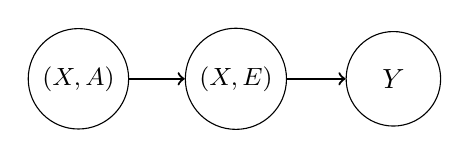
\begin{tikzpicture}

\node[circle,draw, minimum size=1.2cm] (R0) at (0,0) {\begin{small}$(X, A)$\end{small}
};
\node[circle,draw, minimum size=1.2cm] (R1) at (2,0) {\begin{small}$(X, E)$\end{small}};
\node[circle,draw, minimum size=1.2cm] (Y) at (4,0) {$Y$};

\path[->, thick] (R0) edge (R1);
\path[->, thick] (R1) edge (Y);

\end{tikzpicture}
\caption{Bayesian network corresponding to Assumption \ref{assum:indep-mips}.}
\label{fig:embedding_mips}
\vspace{-0.2cm}
% \end{wrapfigure}
\end{figure}


\myparagraph{Intuition}
The context-embedding pair $(X, E)$ can be seen as a representation of the context-action pair $(X, A)$ which contains less `redundant information' regarding the outcome $Y$. Intuitively, the MIPS estimator, which only considers the shift in the distribution of $(X, E)$ is therefore more efficient than the IPW estimator (which considers the shift in the distribution of $(X, A)$ instead). 
% In fact, as the representation $(X, E)$ gets closer to the outcome $Y$ in terms of information content, the variance of the MIPS estimator decreases. We formalise this in Appendix \faaiz{ref}. 

\myparagraph{MR achieves lower variance than MIPS}
Given the intuition above, we should achieve greater variance reduction as the amount of redundant information in the representation $(X, E)$ decreases. We formalise this in Appendix \ref{app:gmips} and show that the variance of MIPS estimator decreases as the representation gets closer to $Y$ in terms of information content. As a result, we achieve the greatest variance reduction by considering the marginal shift in the outcome $Y$ itself (as in MR) rather than the shift in the representation $(X, E)$ (as in MIPS). The following result formalizes this finding. 
% \jef{Ask Arnaud and Rob}
% As such, the greatest variance reduction is achieved when instead of considering the shift in the representation $(X, E)$ as in MIPS, we consider the marginal shift in the outcome $Y$ itself as in the MR estimator. The following results formalises this:
\begin{theorem}\label{prop:mips_main_text}
    When the weights $w(y)$, $\frac{\ptar(e, x)}{\pbeh(e, x)}$ and $\rho(a, x)$ are known exactly, then under Assumption \ref{assum:indep-mips}, 
    \begin{align*}
        \Ebeh[\thetamr] = \Ebeh[\hat{\theta}_{\textup{MIPS}}] = \Etar[Y], \quad \textup{and} \quad \Vbeh[\thetamr] \leq \Vbeh[\hat{\theta}_{\textup{MIPS}}] \leq \Vbeh[\thetaipw].
    \end{align*}
    % \[
    % \Vbeh[\thetamr] \leq \Vbeh[\hat{\theta}_{\textup{MIPS}}] \leq \Vbeh[\thetaipw].
    % \]
\end{theorem}
% \paragraph{Intuition}
This analysis provides a link between the MR and MIPS estimators in the framework of contextual bandits, and shows that the MR estimator achieves lower variance than MIPS estimator while not requiring any additional assumptions (e.g.\ Assumption \ref{assum:indep-mips} as in MIPS). We also verify this empirically in Section \ref{sec:exp-synth} by reproducing the experimental setup in \cite{saito2022off} along with the MR baseline.
% Proposition \ref{prop:mips_main_text} provides us an alternative perspective of the MR estimator. Both, the MIPS and the MR estimators lead to variance reduction by considering a representation of the context-action pair $(X, A)$ which contains less redundant information. However, in the case of the MR estimator, the representation under consideration is the outcome $Y$ itself and therefore it contains precisely the least amount of information necessary to obtain the outcome $Y$. Consequently, the variance of MR estimator is . Additionally, unlike the MIPS estimator, the MR estimator does not require any additional conditional independence assumptions.

% we replace the representation $(X, E)$ by the outcome $Y$ itself. In fact, this recovers the MR estimator.

% In fact, if instead of considering representations of 

% The intuitive reason behind the variance reduction is that the MIPS estimator considers the shift in the joint distribution of $(X, E)$ resulting from the policy shift.

\subsubsection{Weight estimation error}\label{subsec:weight-estimation-error}
% So far our analysis assumes that the behaviour policy $\beh$ and the marginal ratios $w(y)$ are known. However, in practice, both quantities may be unknown and must be estimated from data. To do so, we first split the available logged data $\D$ into training data $\Dtr = \{(x^\tr_i, a^\tr_i, y^\tr_i)\}_{i=1}^m$, which is used for weight estimation, and evaluation data $\Dev = \{(x_i, a_i, y_i)\}_{i=1}^n$, which is used to compute the OPE estimate. 
% % We then estimate the weights $w(y)$ using $\Dtr$ as follows:
% The estimation of weights $w(y)$ involves a two-step process, exclusively utilizing data from $\Dtr$ in each step:
Our analysis so far assumes prior knowledge of the behavior policy $\beh$ and the marginal ratios $w(y)$. However, in practice, both quantities are often unknown and must be estimated from data. To this end, we assume access to an additional training dataset $\Dtr = \{(x^\tr_i, a^\tr_i, y^\tr_i)\}_{i=1}^m$ (for weight estimation), in addition to the evaluation dataset $\D = \{(x_i, a_i, y_i)\}_{i=1}^n$ (for computing the OPE estimate). 
% More generally, these datasets can be obtained by splitting the available logged data.
% we first split the available logged data $\D$ into two subsets: the training data $\Dtr = \{(x^\tr_i, a^\tr_i, y^\tr_i)\}_{i=1}^m$ for weight estimation, and the evaluation data $\Dev = \{(x_i, a_i, y_i)\}_{i=1}^n$ for computing the OPE estimate.
The estimation of $\hat{w}(y)$ involves a two-step process that exclusively utilizes data from $\Dtr$:
% The weights $w(y)$ are then estimated using $\Dtr$ as follows:
% In practice, often the behaviour policy $\beh$ is not known and must be estimated through the logged observational data. 
\begin{enumerate}[label=(\roman*)]
    \item First, we estimate the policy ratio $\hat{\rho}(a, x) \approx \frac{\tar(a | x)}{\beh(a | x)}$. This can be achieved by estimating the behaviour policy $\hatbeh$, and defining $\hat{\rho}(a, x)\coloneqq \frac{\tar(a\mid x)}{\hatbeh(a\mid x)}$. Alternatively, $\hat{\rho}(a, x)$ can also be estimated directly by using density ratio estimation techniques as in \cite{sondhi2020balanced}.
    \item Secondly, we estimate the weights $\hat{w}(y)$ using Eq. \eqref{eq:weights-obj} with $\hat{\rho}$ instead of $\rho$.
\end{enumerate}

    % First, we estimate the behaviour policy $\hatbeh$, and define the policy ratio 
    % $
    % \hat{\rho}(A, X)\coloneqq \frac{\tar(a\mid x)}{\hatbeh(a\mid x)}.$
    % and use it to define the estimated ratios $\hat{\rho}(a, x)\coloneqq \tar(a\mid x)/\hatbeh(a\mid x)$.
 
% In this case, the policy ratio $\rho(a, x)$ is not known, and we resort to the use of estimated ratios $\hat{\rho}(a, x)\coloneqq \tar(a\mid x)/\hatbeh(a\mid x)$ instead.
% % This means the policy ratio $\rho(a, x)$ is not known, and must be estimated using the estimated behaviour policy, i.e.\ $\hat{\rho}(a, x)\coloneqq \tar(a\mid x)/\hatbeh(a\mid x)$. 
% The use of this ratio estimate $\hat{\rho}(a, x)$ may introduce bias in the IPW estimator. This also means that we have to rely on the estimated policy $\hatbeh$ to estimate the marginal ratio $w(y)$, which may also introduce a bias in the MR estimator. 

In practice, one may consider splitting $\Dtr$ for each estimation step outlined above. Moreover,
each approximation step may introduce bias and therefore, the MR estimator may have two sources of bias.
% the MR estimator may have two sources of bias: estimation of the behaviour policy $\hatbeh$, and the estimation of weights $\hat{w}(y)$.
% $$
% \hat{w}(y) \approx \Ebeh[\hat{\rho}(A, X)\mid Y=y] \qquad \textup{where, } \qquad  \hat{\rho}(a, x) \coloneqq \frac{\tar(a\mid x)}{\hatbeh(a\mid x)}.
% $$
While classical OPE methods like IPW and DR also suffer from bias because of $\hat{\rho}$ estimation, the estimation of $\hat{w}(y)$ is specific to MR. However, we show below
that given any policy ratio estimate $\hat{\rho}$, if $\hat{w}(y)$ approximates $\Ebeh[\hat{\rho}(A, X)\mid Y=y]$ `well enough' (i.e., the estimation step (ii) shown above is `accurate enough'), 
then MR achieves a lower variance than IPW and incurs little extra bias.

\begin{proposition}\label{prop:bias-and-var-main}
Suppose that the IPW and MR estimators are defined as,
\[
\approxipw \coloneqq \frac{1}{n}\sum_{i=1}^n\hat{\rho}(a_i, x_i)\, y_i, \quad \textup{and }\quad \approxmr \coloneqq \frac{1}{n}\sum_{i=1}^n\hat{w}(y_i)\, y_i,
\]
and define the approximation error as $\epsilon \coloneqq \hat{w}(Y) - \tilde{w}(Y)$, where $\tilde{w}(Y) \coloneqq \Ebeh[\hat{\rho}(A, X)\mid Y]$. Then we have that, $\textup{Bias}(\approxmr) - \textup{Bias}(\approxipw) = \Ebeh[\epsilon\,Y]$. Moreover,
% $\Ebeh[\epsilon] = 0$ and 
% $\epsilon \indep Y$. Then, 
% \begin{align*}
%     \textup{Bias}(\thetamr) &= \textup{Bias}(\thetaipw) \quad \textup{and,} \\
%     n (\Vbeh[\thetaipw] - \Vbeh[\thetamr]) 
%     &= \E_{Y\sim \pbeh(Y)} \left[ \Vbeh\left[ \hat{\rho}(A, X) \mid Y \right]\, Y^2 \right] - \Vbeh[\epsilon]\,\Ebeh[Y^2].
% \end{align*}
\begin{small}
\begin{align}
    \Vbeh[\approxipw] - \Vbeh[\approxmr]
    % &= \frac{1}{n}\left(\underbrace{\Ebeh[\Vbeh[\hat{\rho}(A, X)\,Y\mid Y]]}_{\geq 0} - \Vbeh[\epsilon\,Y] - 2\,\textup{Cov}(\tilde{w}(Y)\,Y, \epsilon\,Y)\right). \label{eq:var-difference-approximate-weights}
    &= \frac{1}{n}(\underbrace{\Ebeh[\Vbeh[\hat{\rho}(A, X)\,Y\mid Y]]}_{\geq 0} - \Vbeh[\epsilon\,Y] - 2\,\textup{Cov}(\tilde{w}(Y)\,Y, \epsilon\,Y)). \label{eq:var-difference-approximate-weights}
\end{align}
\end{small}
% and,
% \begin{align*}
%     &n (\Vbeh[\approxipw] - \Vbeh[\approxmr]) \\
%     &\quad= \Ebeh[\Vbeh[\hat{\rho}(A, X)\mid Y]\,Y^2] - \Vbeh[\epsilon\,Y] - 2\,\textup{Cov}(\Ebeh[\hat{\rho}(A, X)\mid Y]\,Y, \epsilon\,Y).
% \end{align*}
\end{proposition}
% if $\Ebeh[\hat{\rho}(A, X)\mid Y]$ is estimated `well enough', MR achieves a lower variance than IPW and does not incur any extra bias compared to IPW.
\myparagraph{Intuition} The $\epsilon$ term defined in Proposition \ref{prop:bias-and-var-main} denotes the error of the second approximation step outlined above. 
As a direct consequence of this result, we show in Appendix \ref{sec:wide_nns_weight_estimation} that as the error $\epsilon$ becomes small (specifically as $\Ebeh[\epsilon^2]\rightarrow 0$), the difference between biases of MR and IPW estimator becomes negligible.
% The result shows that as the error $\epsilon$ becomes small, i.e. $\epsilon \overset{\textup{a.s.}}{\rightarrow}0$, the difference between biases of MR and IPW estimator decreases. 
Likewise, the terms $\Vbeh[\epsilon\,Y]$ and $\textup{Cov}(\tilde{w}(Y)\,Y, \epsilon\,Y)$ in Eq. \eqref{eq:var-difference-approximate-weights} will also be small and as a result the variance of MR will be lower than that of IPW (as the first term is positive). 

In fact, using recent results regarding the generalisation error of neural networks \citep{lai2023generalization}, we show that when using 2-layer wide neural networks to approximate the weights $\hat{w}(y)$, the estimation error $\epsilon$ declines with increasing training data size $m$. Specifically, under certain regularity assumptions we obtain $\Ebeh[\epsilon^2] = O(m^{-2/3})$. Using this we show that as the training data size $m$ increases, the biases of MR and IPW estimators become roughly equal with a high probability, and
\[
\Vbeh[\approxipw] - \Vbeh[\approxmr] = \frac{1}{n}\,\Ebeh[\Vbeh[\hat{\rho}(A, X)\,Y\mid Y]] + O(m^{-1/3}).
\]
Therefore the variance of MR estimator falls below that of IPW for large enough $m$. The empirical results shown in Appendix \ref{subsec:mips-empirical} are consistent with this result. Due to space constraints, the main technical result has been included in Appendix \ref{sec:wide_nns_weight_estimation}.

% number of training samples $m$ increases, the biases of MR and IPW estimators become roughly equal, whereas the variance of MR estimator falls below that of the IPW estimator. The empirical results shown in Appendix \ref{subsec:additional-experiments} are consistent with this result.
% Moreover, in Theorem \ref{prop:informal}, the estimated policy ratio $\hat{\rho}(a, x)$ is fixed for increasing $m$, i.e., we do not update $\hat{\rho}(a, x)$ as more training data becomes available. While this may seem as a disadvantage for the IPW estimator, we point out that the result also holds when the policy ratio is exact (i.e., $\hat{\rho}(a, x) = \rho(a, x)$) and hence the IPW estimator is unbiased.

% In fact, using recent results regarding the generalisation error of wide neural networks \citep{lai2023generalization}, we can show that when using 2-layer wide neural networks to approximate the weights $\hat{w}(y)$, the estimation error of the second approximation step above scales as $O(m^{-1/3})$ where $m$ is the number of training data used to approximate $\hat{w}(y)$.
% % Using recent results regarding the generalisation error of wide neural networks \citep{lai2023generalization}, we show that when using 2-layer wide neural networks to approximate the weights $\hat{w}(y)$, then under mild assumptions, $\Ebeh[\epsilon^2]\leq O(m^{-2/3})$. Here $m$ is the number of training data used to approximate $\hat{w}(y)$. 
% Due to space constraints, we include an informal statement of the result here. The main technical result has been included in Appendix \ref{sec:wide_nns_weight_estimation}.

% \begin{theorem}[Informal Statement]\label{prop:informal}
% % Let $\mathcal{D}_{tr}$ be training data with $m$ samples $\{(x^\tr_i, a^\tr_i, y^\tr_i)\}_{i=1}^m$.
% Suppose that the IPW and MR estimators are defined as,
% \[
% \approxipw \coloneqq \frac{1}{n}\sum_{i=1}^n\hat{\rho}(a_i, x_i)\, y_i, \quad \textup{and }\quad \approxmr \coloneqq \frac{1}{n}\sum_{i=1}^n\hat{w}(y_i)\, y_i,
% \]
% % and let
% % \[
% % \thetamr = \frac{1}{n}\sum_{i=1}^n\hat{w}(y_i)\, y_i,
% % \]
% where $\hat{w}(y)$ is approximated by minimising the following empirical loss on a training dataset of size $m$, $\mathcal{D}_{tr}\coloneqq \{(x^\tr_i, a^\tr_i, y^\tr_i)\}_{i=1}^m$ (disjoint from evaluation dataset $\{(x_i, a_i, y_i)\}_{i=1}^n$):
% % \[
% %     \mathcal{L}(\theta) = \E_{\mathcal{D}_{tr}}(\hat{\rho}(A, X) - f_\phi(Y))^2.
% % \]
% \[
%     \mathcal{L}(\phi) = \E_{(X, A, Y)\sim \mathcal{D}_{tr}} \left[\left(\hat{\rho}(A, X) - f_{\phi}(Y)\right)^2\right].
% \]
% If $f_\phi$ is a two-layer neural network with large enough width and for sufficiently large $m$, then under the regularity assumptions provided in Appendix \ref{sec:wide_nns_weight_estimation}, the following holds with high probability,
% \begin{align*}
%     |\textup{Bias}(\approxmr) - \textup{Bias}(\approxipw)| &= O(m^{-1/3}),\\
%     \Vbeh[\approxipw] - \Vbeh[\approxmr] &= \frac{1}{n}\underbrace{\Ebeh[\Vbeh[\hat{\rho}(A, X)\mid Y]\, Y^2]}_{\geq 0} + O(m^{-2/3}).
% \end{align*}
% % holds with high probability. 
% \end{theorem}

% \myparagraph{Intuition} This theorem shows that as the number of training samples $m$ increases, the biases of MR and IPW estimators become roughly equal, whereas the variance of MR estimator falls below that of the IPW estimator. The empirical results shown in Appendix \ref{subsec:additional-experiments} are consistent with this result.
% Moreover, in Theorem \ref{prop:informal}, the estimated policy ratio $\hat{\rho}(a, x)$ is fixed for increasing $m$, i.e., we do not update $\hat{\rho}(a, x)$ as more training data becomes available. While this may seem as a disadvantage for the IPW estimator, we point out that the result also holds when the policy ratio is exact (i.e., $\hat{\rho}(a, x) = \rho(a, x)$) and hence the IPW estimator is unbiased.
 
% In this section, we show that under certain assumptions, the use of the estimated importance weights $\hat{w}(y)$ rather than $\hat{\rho}(a, x)$ does not worsen the bias of the resulting OPE estimator. Moreover, if $\hat{w}(y)$ are estimated `well enough', the variance of MR estimator will be lower than that of IPW estimator in this case as well. The following result formalises this:
% \begin{align}
%     \hat{w} = \arg\min_{f} \, \Ebeh \Bigg[\frac{\tar(A|X)}{\hatbeh (A|X)}-f(Y)\Bigg]^2, \label{eq:estimated-marginal-ratio}
% \end{align}
% then the bias in the MR estimator will be equal to the bias in the IPW estimator. This means that in the case when $\beh$ is approximated and the marginal ratio estimate $\hat{w}(y)$ are obtained by exactly regressing to the approximate policy ratios $\hat{\rho}(a, x)$, the biases of the MR and IPW estimators will be identical. Additionally, the result in Proposition \ref{prop:var_mr} straightforwardly extends to this case, showing that if the marginal ratios $\hat{w}(y)$ are estimated `well enough', the variance of MR estimator will be lower than that of IPW estimator in this case as well.

\subsection{Application to causal inference}\label{subsec:application-to-causal-inference}
 Beyond contextual bandits, the variance reduction properties of the MR estimator make it highly useful in a wide variety of other applications. Here, we show one such application in the field of causal inference, where MR can be used for the estimation of average treatment effect (ATE) \citep{pearl2009causality} and leads to some desirable properties in comparison to the conventional ATE estimation approaches. Specifically, we illustrate that the MR estimator for ATE utilizes the evaluation data $\D$ more efficiently and achieves lower variance than state-of-the-art ATE estimators and consequently provides more accurate ATE estimates.
% leads to a significantly more data efficient methodology with  
% This comparative advantage of MR becomes even more apparent when the observational data size is small.
% We show, both theoretically and empirically, that our methodology provides more reliable ATE estimation overall, and performs especially better than other baselines when the number of data is low.
% The MR estimator can also be applied in the setting of causal inference for estimation of average treatment effect (ATE) and leads to more data efficient methodology than many state-of-the-art ATE estimators.
To be concrete, the goal in this setting is to estimate ATE, defined as follows:
% Off-Policy evaluation is widely applied sin causal inference, where often the goal is to estimate the average treatment effect (ATE), defined as follows:
\[
\ate \coloneqq \E[Y(1)-Y(0)].
\]
Here $Y(a)$ corresponds to the outcome under a deterministic policy $\pi_a(a'\mid x) \coloneqq \ind(a'=a)$. Hence any OPE estimator can be used to estimate $\E[Y(a)]$ (and therefore ATE) by considering target policy $\tar = \pi_a$.
% Given an OPE estimator, $\E[Y(a)]$ 
% We can use any OPE estimator with deterministic target policies to estimate the ATE. 
% We provide explicit expressions of ATE estimators using MR, IPW and DR in Appendix \ref{app:causal-inference}.
An important distinction between MR and existing approaches (like IPW or DR) is that, when estimating $\E[Y(a)]$, the existing approaches only use datapoints in $\D$ with $A=a$. To see why this is the case, we note that the policy ratios $\frac{\tar(A|X)}{\beh(A|X)} = \frac{\ind(A=a)}{\beh(A|X)}$ are zero when $A\neq a$. In contrast, the MR weights $\frac{\ptar(Y)}{\pbeh(Y)}$ are not necessarily zero for datapoints with $A\neq a$, and therefore the MR estimator uses all evaluation datapoints when estimating $\E[Y(a)]$. 

As such we show that MR applied to ATE estimation leads to a smaller variance than the existing approaches. Moreover, because MR is able to use all datapoints when estimating $\E[Y(a)]$, MR will generally be more accurate than the existing methods especially in the setting where the data is imbalanced, i.e., the number of datapoints with $A=a$ is small for a specific action $a$.
In Appendix \ref{app:causal-inference}, we formalise this variance reduction of the MR ATE estimator compared to IPW and DR estimators, by deriving analogous results to Propositions \ref{prop:var_mr} and \ref{prop:var_dr}. In addition, we also show empirically in Section \ref{subsec:causal-experiments} that the MR ATE estimator outperforms the most commonly used ATE estimators.
\begin{comment}

\begin{proposition}\label{prop:bias-and-var}
Let 
\[
\thetaipw = \frac{1}{n}\hat{\rho}(a_i, x_i)\, y_i,
\]
where $\hat{\rho}(a, x)\coloneqq \tar(a\mid x)/\hatbeh(a\mid x)$. Additionally, let
\[
\thetamr = \frac{1}{n}\hat{w}(y_i)\, y_i,
\]
where $\hat{w}(y)$ satisfies Eq. $\eqref{eq:estimated-marginal-ratio}$. Then, 
\begin{align*}
    \textup{Bias}(\thetamr) &= \textup{Bias}(\thetaipw) \qquad \textup{and,} \\
    n (\Vbeh[\thetaipw] - \Vbeh[\thetamr]) 
    &= \E_{Y\sim \pbeh(Y)} \left[ \Vbeh\left[ \hat{\rho}(A, X) \mid Y \right]\, Y^2 \right].
\end{align*}
\end{proposition}
More generally, if $\hat{w}$ is a `noisy' estimate of the conditional expectation $\Ebeh[\hat{\rho}(A, X)\mid Y]$, we can obtain similar results regarding the bias and variance of the MR estimators under certain assumptions. 
\end{comment}


% Using recent results regarding the generalisation error of wide neural networks \citep{lai2023generalization}, we show that when using 2-layer wide neural networks to approximate the weights $\hat{w}(y)$, then under mild assumptions, $\Ebeh[\epsilon^2]\leq O(m^{-2/3})$. Here $m$ is the number of training data used to approximate $\hat{w}(y)$. Due to space constraints, we include an informal statement of the result here. The main technical result has been included in Appendix \ref{sec:wide_nns_weight_estimation}.

% Additionally, replacing the true behaviour policy $\beh$ by the estimate $\hatbeh$ in Eq. \eqref{eq:weights-obj} will 

% if we approximate the marginal ratio $w(y)$ using the approximate 



\begin{comment}
    

Specifically, the traditional IPW estimator applied to ATE estimation yields:
\[
\ateipw = \frac{1}{n} \sum_{i=1}^n \rho_{\ate}(a_i, x_i) \times y_i, \qquad \textup{where, } \qquad \rho_{\ate}(a, x) \coloneqq \frac{\mathbbm{1}(a=1) - \mathbbm{1}(a=0)}{\beh (a|x)}.
\]

Simlarly, the MR estimator can be written as
$$
\atemr = \frac{1}{n}\sum_{i=1}^n w_{\ate}(y_i)\times y_i, \qquad \textup{where, } \qquad w_{\ate}(y) = \frac{p_{\pi^{(1)}}(y) - p_{\pi^{(0)}}(y)}{\pbeh(y)},
$$ 
and $\pi^{(a)}(a'\mid x) \coloneqq \mathbbm{1}(a'=a)$ for $a\in \{0,1\}$, and $w_{\ate}(y)$ can be estimated using regression similar to Eq. \eqref{eq:weights-obj}.
\end{comment}
% Again, using the fact that $w_{\ate}(Y) \eqas \E[\rho_{\ate}(A, X)\mid Y]$, we can obtain $w_{\ate}$ by minimising a simple mean-squared loss:
% \begin{align*}
%     w_{\ate} =\arg \min_{f} \Ebeh \Big[\frac{\mathbbm{1}(A=1)- \mathbbm{1}(A=0)}{\beh (A|X)}-f(Y)\Big]^2
% \end{align*}

% For the MR estimator, we don't need to estimate weights for $Y(1)$ and $Y(0)$ separately, as we can combine the two as follows:
% \begin{align}
%     w_{\ate} =\arg \min_{f} \Ebeh \Big[\frac{\mathbbm{1}(A=1)- \mathbbm{1}(A=0)}{\beh (A|X)}-f(Y)\Big]^2 \label{eq:ate-weights-loss}
% \end{align}
% It follows straightforwardly from Lemma \ref{prop:weights-est}, that the function that minimises  \eqref{eq:ate-weights-loss} is equal to 
% \[
% w_{\ate}(y) = \frac{p_{\pi^{(1)}}(y) - p_{\pi^{(0)}}(y)}{\pbeh(y)},
% \] 
% where $\pi^{(a)}(a'\mid x) \coloneqq \mathbbm{1}(a'=a)$ for $a\in \{0,1\}$.
% Then, the MR estimator can be written as
% $$\atemr = \frac{1}{n}\sum_{i=1}^n w_{\ate}(y_i)\times y_i.$$ 
% In contrast, the traditional IPW estimator is of the form:
% \[
% \ateipw = \frac{1}{n} \sum_{i=1}^n \rho_{\ate}(a_i, x_i) \times y_i,
% \]
% where 
% \[
% \rho_{\ate}(a, x) \coloneqq \frac{\mathbbm{1}(a=1) - \mathbbm{1}(a=0)}{\beh (a|x)}.
% \]

\section{Related Work}
Off-Policy evaluation is a central problem both in contextual bandits \citep{dudik2014doubly, wang2017optimal, liu2018breaking, farajtabar2018more, su2019continuous, su2020doubly, kallus2021optimal, metelli2021subgaussian, saito2020open} and in RL \citep{thomas2016data, xie2019advances, kallus2020off, liu2020understanding}. 
Existing OPE methodologies can be broadly categorised into Direct Method (DM), Inverse Probability Weighting (IPW), and Doubly Robust (DR). 
While DM typically has a low variance, it suffers from high bias when the reward model is misspecified \citep{voloshin2021empirical}. 
On the other hand, IPW \citep{horvitz1952generalization} and DR \citep{dudik2014doubly, wang2017optimal, su2020doubly} use policy ratios as importance weights when estimating policy value and suffer from high variance as overlap between behaviour and target policies increases or as the action/context space gets larger \citep{sachdeva2020off, saito2022off}. To circumvent this problem, techniques like weight clipping or normalisation \citep{swaminathan2015counterfactual, swaminathan2015the, chaudhuri2019london} are often employed, however, these can often increase bias.

% The IPW estimator \citep{horvitz1952generalization} can have low bias but suffers from high variance as overlap between behaviour and target policies increases or as the action/context space gets larger \citep{sachdeva2020off, saito2022off}. To circumvent this problem, techniques like weight clipping or normalisation \citep{swaminathan2015counterfactual, swaminathan2015the} are often employed, however, these can often lead to the worsening of bias.



% The second class of methodologies, called the Inverse Probability Weighting (IPW) \citep{horvitz1952generalization}, uses importance weights to estimate the value of the target policy. If the behaviour policy is well-estimated, the IPW estimator will have a low bias. However, IPW can suffer from a high variance especially as the overlap between behaviour and target policies increases, or as the size of action and/or context space increases \citep{sachdeva2020off}. To circumvent this problem, techniques like weight clipping or normalisation \citep{swaminathan2015counterfactual, swaminathan2015the} are often employed, however, these can often lead to the worsening of bias. 

% The DR method \citep{dudik2014doubly} and its extensions \citep{wang2017optimal, su2020doubly} combine the direct method with importance sampling and achieves better overall bias and variance than the IPW method. However, like the IPW method these DR methods also take the shift of joint distributions of $(X, A, Y)$ into consideration when estimating policy value. As we show in Section \ref{subsec:comparison}, this can lead to high variance especially as the policy shift increases or the action and/or context space gets larger. 

In contrast to these approaches, \cite{saito2022off} propose MIPS, which considers the marginal shift in the distribution of a lower dimensional embedding of the action space. While this approach reduces the variance associated with IPW, we show in Section \ref{subsec:mips-comparison} that the MR estimator achieves a lower variance than MIPS while not requiring any additional assumptions (like Assumption \ref{assum:indep-mips}).
% it requires conditional independence assumptions on the embedding $R$, the violation of which may lead to high bias. 
% We show in Section \ref{subsec:mips-comparison} that in comparison, the MR estimator does not require any such conditional independence assumptions, and achieves a lower variance than the MIPS estimator by only considering the shift in the marginal distribution of the reward $Y$. 

In the context of Reinforcement Learning (RL), various marginalisation techniques of importance weights have been used to propose OPE methodologies.
% OPE methodologies using marginalised importance weighting have been proposed 
% \citep{liu2018breaking, xie2019advances, Fujimoto2021deep, rowland2020conditional}
% \citep{thomas2016data, xie2019advances, kallus2020off, liu2020understanding}. 
\cite{liu2018breaking, xie2019advances, kallus2020off} use methods which considers the shift in the marginal distribution of the states, and applies importance weighting with respect to this marginal shift rather than the trajectory distribution. Similarly, \cite{Fujimoto2021deep} use marginalisation for OPE in deep RL, where the goal is to consider the shift in marginal distributions of state and action. Although marginalization is a key trick of these estimators, these techniques do not consider the marginal shift in reward as in MR and are aimed at resolving the curse of horizon, a problem specific to RL. Apart from this, \cite{rowland2020conditional} propose a general framework of OPE based on conditional expectations of importance ratios for variance reduction. While their proposed framework includes reward conditioned importance ratios, this is not the main focus and there is little theoretical and empirical comparison of their proposed methodology with existing state-of-the-art methods like DR. 

Finally we note that the idea of approximating the ratio of intractable marginal densities via leveraging the fact that this ratio can be reformulated as the conditional expectation of a ratio of tractable densities is a standard idea in computational statistics \cite{meng1996simulating} and has been exploited more recently to perform likelihood-free inference \cite{brehmer2020mining}. In particular, while  \cite{meng1996simulating} typically approximates this expectation through Markov chain Monte Carlo, \cite{brehmer2020mining} uses regression instead, however without any theory.
% of this approach has been carried out in \cite{brehmer2020mining}.

% Our work introduces the marginal ratio estimator for OPE in contextual bandits. We provide extensive theoretical and empirical comparisons of our proposed estimator with existing methods, and show that the MR estimator performs especially better than the other methods in large actions and/or context spaces. 
% \faaiz{@Arnaud and Rob: what are your thoughts about this characterisation of \cite{rowland2020conditional}?}

% Our work proposes an OPE methodology for contextual bandits which only considers the shift in the marginal distribution of rewards. In addition, we include extensive theoretical and empirical comparisons of our proposed estimator with existing methods, and show that the MR estimator performs especially better than the other methods in large actions and/or context spaces. 

\begin{comment}
\begin{itemize}
    \item IPW
    \item Double robust methods
    \item Debiased methods 
    \item See related works in \cite{saito2022off}
\end{itemize}
\subsection{Baselines in Contextual Bandits setting}
\begin{itemize}
    \item \cite{thomas2016data, saito2021evaluating, saito2022off,wang2017optimal}
    \item Using ideas from \cite{saito2022off},  we can show that our methodology requires common support of $\pbeh(Y\mid X)$ and $\ptar(Y\mid X)$ which is weaker than requiring common supports of $\beh(A\mid X)$ and $\tar(A\mid X)$, which is needed for IPW estimator. We can show that our estimator has a smaller variance than the methodology proposed by \cite{saito2022off}. Moreover, we should show empirically that, as a consequence of this, our estimator is more robust to heavy-tailed policy ratios. The baselines considered in this paper are the ones to compare against.
    \item \cite{wang2017optimal} proposes a SWITCH estimator for policy evaluation, and show that this estimator is minimax optimal when the hyperparameter $\tau$ is chosen appropriately. Moreover, this estimator is more robust to large (or heavy-tailed) importance weights. It also includes an expression for the variance of the DR estimator which could be useful.
    \item \cite{saito2021evaluating}: In this work, the authors develop Interpretable Evaluation for Offline Evaluation (IEOE), an experimental procedure to evaluate OPE estimators’ robustness to changes in hyperparameters and/or evaluation policies in an interpretable manner. This is more of a review paper.
    \item \cite{liu2019triply}: Could be an interesting baseline. The background section of this paper seems interesting. 
\end{itemize}
\subsection{Marginalised Importance Sampling in Reinforcement Learning}
The main difference between this line of work and our idea is that these works consider the marginal distribution over the states. Instead, we propose considering the marginal distribution over rewards directly. 
\begin{itemize}
    \item \cite{liu2018breaking}: The paper originally proposed avoiding the long horizon problem by computing MIS over state distributions rather than entire trajectories. The marginal ratio in these works is different to ours.  
    \item \cite{Fujimoto2021deep}: Applies the MIS idea to deep RL setting: Marginalized importance sampling (MIS), which measures the density ratio between the state-action occupancy of a target policy and that of a sampling distribution, is a promising approach for off-policy evaluation. However, current state-of-the-art MIS methods rely on complex optimization tricks and succeed mostly on simple toy problems. This paper bridges the gap between MIS and deep reinforcement learning by observing that the density ratio can be computed from the successor representation of the target policy. 
    \item \cite{kallus2020off}: The related works section of this paper is very useful. In this work, the authors propose the use of a marginal importance sampling estimator which is somewhat similar to ours (although not the same). Would be useful to read this in depth.
    \item \cite{xie2019advances}: Avoiding the long horizon problem by computing IS over state distributions rather than trajectories - was already introduced in \cite{liu2018breaking}, which the authors cite sufficiently often in the text. However, the approach the authors take to leveraging this idea is original. The estimation technique for the ratios is also different -- the authors propose a recursive estimation technique to estimate the marginal distribution ratios over states. 
    \item \cite{liu2020understanding} also references MIS estimators. 
    \item \cite{rowland2020conditional}: This paper proposes conditional importance sampling for variance reduction in RL setting. The paper considers a general conditioning strategy, based on conditioning importance weights on different statistics. They also mention reward conditional importance sampling. \textbf{Important paper.} 
\end{itemize}
\end{comment}


\section{Empirical Evaluation}
In this section, we provide empirical evidence to support our theoretical results by investigating the performance of our MR estimator against the current state-of-the-art OPE methods. The code to reproduce our experiments has been made available at: \href{https://github.com/faaizT/MR-OPE}{\textcolor{blue}{github.com/faaizT/MR-OPE}}.
% Here, we present a synthetic data experiment and also consider an application of MR to causal inference. 
% Additional experiments that support our proposed method MR on real-world classification datasets are provided in Appendix \ref{app:experiments} due to space constraints. \faaiz{Squeeze in classification exps in main}
% We first consider a synthetic setup to conduct extensive ablation study
% We evaluate MR estimator on synthetic data to identify the cases where it offers more accurate off-policy evaluation. These experiments are conducted using the \emph{OpenBanditPipeline} (OBP)
% % \footnote{\url{https://github.com/st-tech/zr-obp}}
% , an open-source package for OPE developed by \cite{saito2020open}.

\subsection{Experiments on synthetic data}\label{sec:exp-synth}
For our synthetic data experiment, we reproduce the experimental setup for the synthetic data experiment in \cite{saito2022off} by reusing their code with minor modifications.
% We use synthetically generated dataset for this experiment. 
Specifically, $\Xspace \subseteq \mathbb{R}^d$, for various values of $d$ as described below. Likewise, the action space $\Aspace = \{0, \dots, n_a-1\}$, with $n_a$ taking a range of different values. Additional details regarding the reward function, behaviour policy $\beh$, and the estimation of weights $\hat{w}(y)$ have been included in Appendix \ref{subsec:mips-empirical} for completeness. 

% $d$-dimensional context vectors $x$ are sampled from a standard normal distribution, i.e.\ $\Xspace \subseteq \mathbb{R}^d$, for various values of $d$ as described below. Likewise, the action space is finite and comprises of $n_a$ actions, i.e.\ $\Aspace = \{0, \dots, n_a-1\}$, with $n_a$ taking a range of different values. 
% Due to space constraints, we include additional details regarding the reward function, behaviour policy $\beh$, and the estimation of weights $\hat{w}(y)$ in Appendix \ref{sec:app-additional-results}. 


\myparagraph{Target policies} 
To investigate the effect of increasing policy shift, we define a class of policies,
\[
% \vspace{-0.05cm}
\pi^{\alpha^\ast}(a | x) = \alpha^\ast\,\ind(a = \arg\max_{a'\in \Aspace} q(x, a')) + \frac{1-\alpha^\ast}{|\Aspace|} \quad \textup{where} \quad q(x, a) \coloneqq \E[Y\mid X=x, A=a],
% \vspace{-0.05cm}
\]
where $\alpha^\ast \in [0, 1]$ allows us to control the shift between $\beh$ and $\tar$. In particular, as we show later, the shift between $\beh$ and $\tar$ increases as $\alpha^\ast \rightarrow 1$. Using the ground truth behaviour policy $\beh$, we generate a dataset which is split into training and evaluation datasets of sizes $m$ and $n$ respectively. 


% \paragraph{Reward function}
% The expected reward $q(x, a)\coloneqq\E[Y\mid x, a]$ for these experiments is defined as follows:
% \[
%     q(x, a) = \sin \left(a \cdot ||x||_2 \right). 
% \]
% The reward $Y$ is obtained by adding a normal noise random variable to $q(x, a)$
% \[
% Y = q(X, A) + \epsilon, 
% \]
% where $\epsilon \sim \mathcal{N}(0, 0.01)$.

% \paragraph{Behaviour and target policies}
% We first define a behaviour policy by applying softmax function to $q(x, a)$ as
% \[
% \beh(a\mid x) = \frac{\exp{(q(x, a))}}{\sum_{a' \in \Aspace} \exp{(q(x, a'))}}.
% \]

% where $\beta$ controls the optimality and entropy of the policy $\pi_\beta$. A large positive value of $\beta$ leads to a near-deterministic and well-performing policy, while lower values make the policy increasingly worse and `noisy'. 
% In this experiment, we define the behaviour policy as $\beh = \pi_{\beta^b}$ for $\beta^b = 0.5$ and target policies as $\tar= \pi_{\beta^\ast}$ for $\beta^\ast \in \{0.0, 0.5, 1.0, \ldots, 5.0 \}$.
% In contrast, for the target policy, we define the class of parametric policies,
% \[
% \pi^{\alpha^\ast}(a | x) = \alpha^\ast\,\ind(a = \arg\max_{a'\in \Aspace} q(x, a')) + \frac{1-\alpha^\ast}{|\Aspace|},
% \]
% where $\alpha^\ast \in [0, 1]$ controls the quality of $\pi^{\alpha^\ast}$. In particular, as $\alpha^\ast \rightarrow 1$, the target policy approaches the optimal policy. 


\myparagraph{Baselines} 
We compare our estimator with DM, IPW, DR and MIPS estimators. Our setup includes action embeddings $E$ satisfying Assumption \ref{assum:indep-mips}, and so MIPS is unbiased.
% Since there is no natural action embedding $E$ in our setup which satisfies Assumption \ref{assum:indep-mips}, we instead consider a generalised version of MIPS (defined as G-MIPS in Appendix \ref{app:gmips}) which uses an embedding of context-action pair $(X, A)$ rather than an embedding of the action $A$.
% \footnote{We also compare against the original MIPS estimator in Appendix \ref{subsec:mips-empirical} by reproducing the setup of \cite{saito2022off}}
Additional baselines have been considered in Appendix \ref{subsec:mips-empirical}.
For MR, we split the training data to estimate $\hatbeh$ and $\hat{w}(y)$, whereas for all other baselines we use the entire training data to estimate $\hatbeh$ for a fair comparison.
% In addition, we also consider Switch-DR \citep{wang2017optimal} and DR with Optimistic Shrinkage (DRos) \citep{su2020doubly}. 
% To estimate $\hat{q}(x, a)$ for DM and DR estimators, we use multi-layer perceptrons (MLPs). \jef{last sentence not needed}
% \jef{I personally think having the legend at the top is better as now it is asymetric ... not a big deal though lol (fig2)
% }
\begin{figure}[t]
     \centering
     \begin{subfigure}[b]{0.5\textwidth}
         \centering
         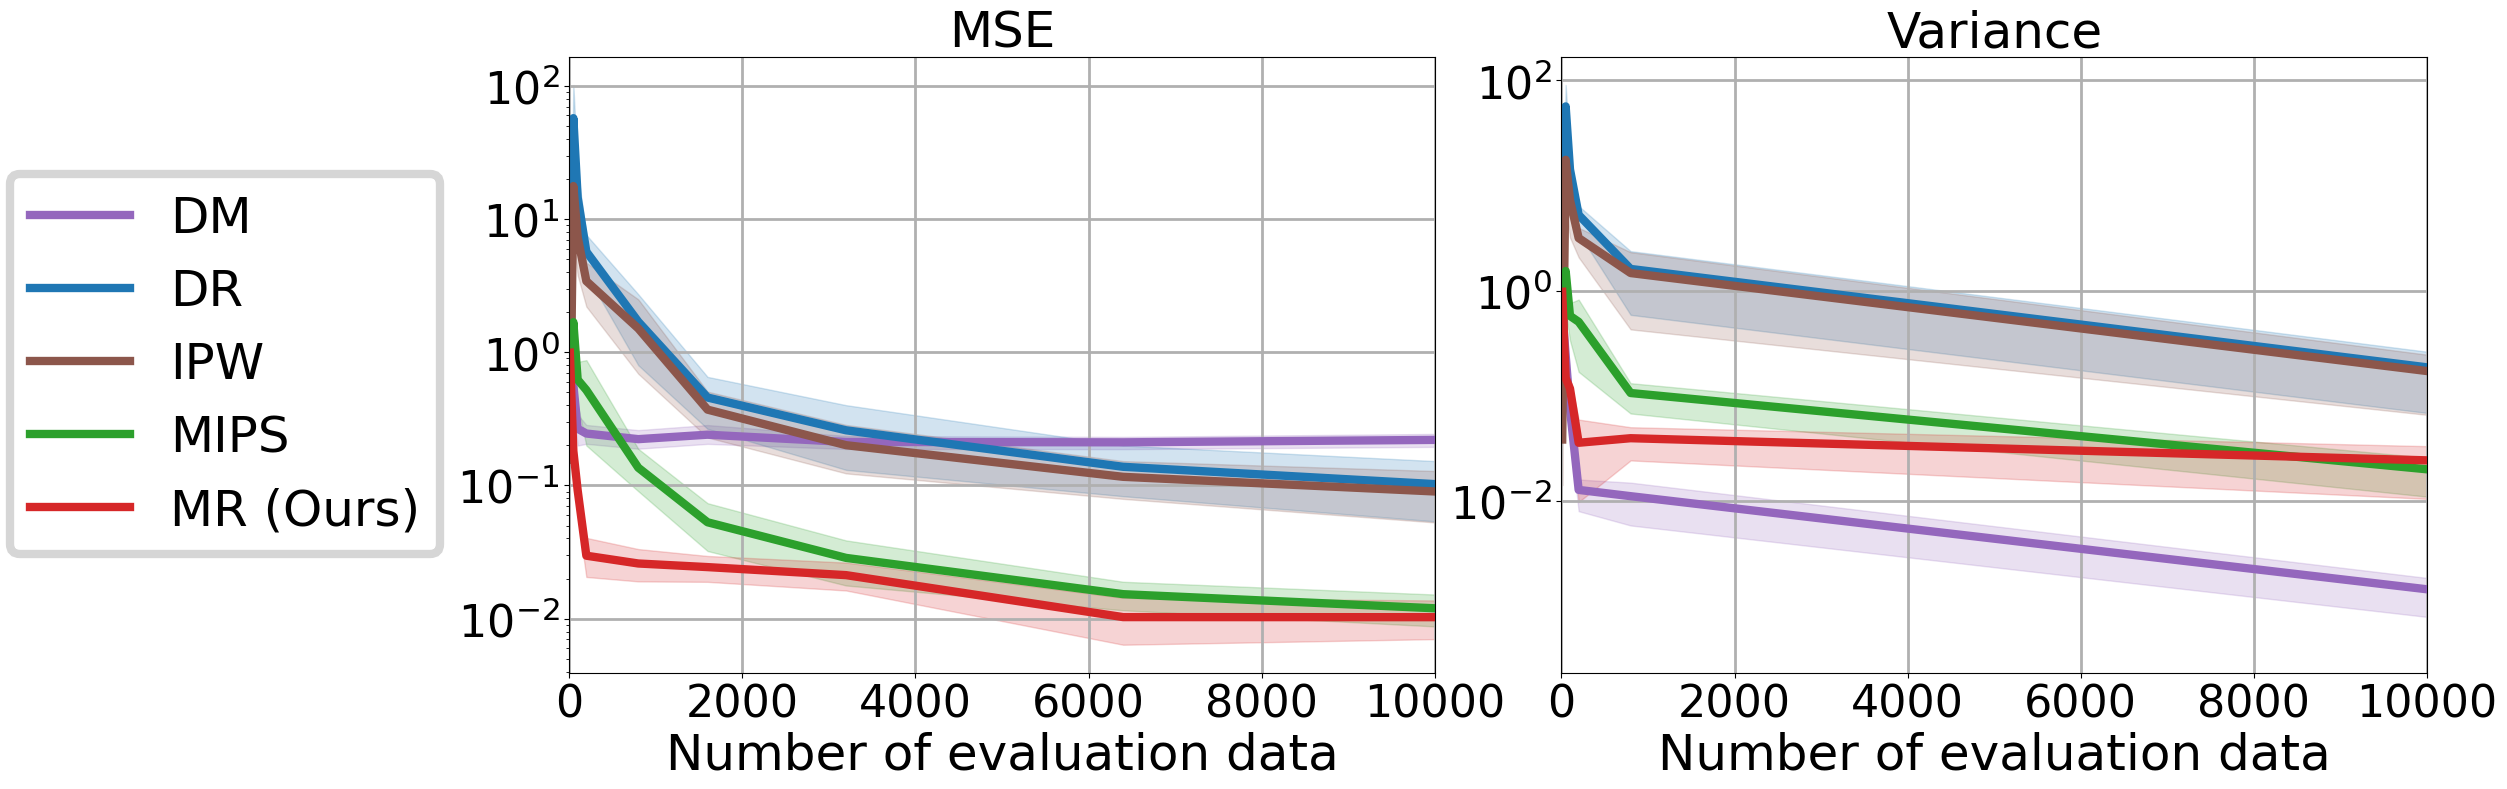
\includegraphics[height=1.06in]{figures/mr/ope_vs_neval_nac_100_alphatar_0_8_dimc_1000_untrunc.png}
         \caption{Results with varying evaluation data size $n$.}
         \label{fig:mse-vs-neval}
     \end{subfigure}%
     \begin{subfigure}[b]{0.5\textwidth}
         \centering
         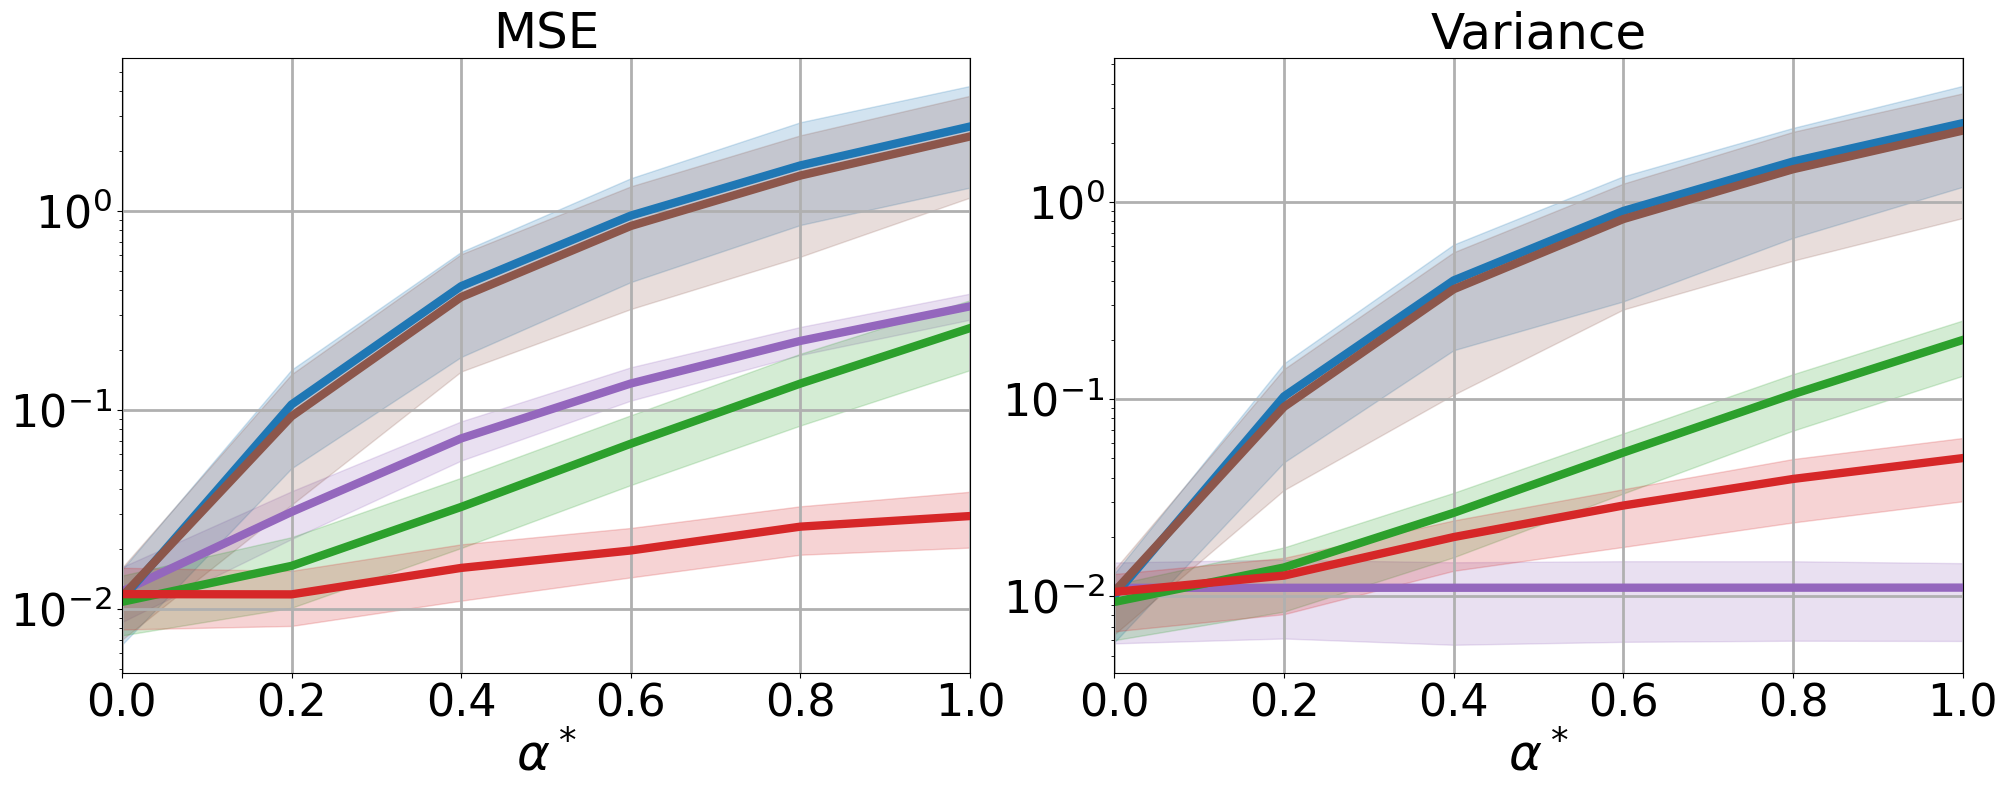
\includegraphics[height=1.06in]{figures/mr/ope_vs_alphatar_nac_100_neval_800_dimc_1000.png}
         \caption{Results with varying $\alpha^\ast$.}
         \label{fig:mse-vs-betatar}
     \end{subfigure}\\
    \caption{Results for synthetic data experiment. In \ref{fig:mse-vs-neval} we have $\alpha^\ast=0.8$ and in \ref{fig:mse-vs-betatar} we have $n = 800$.}
    \label{fig:syn_results1}
\end{figure}

% \begin{figure}[t]
%      \centering
%      \begin{subfigure}[b]{1\textwidth}
%          \centering
%          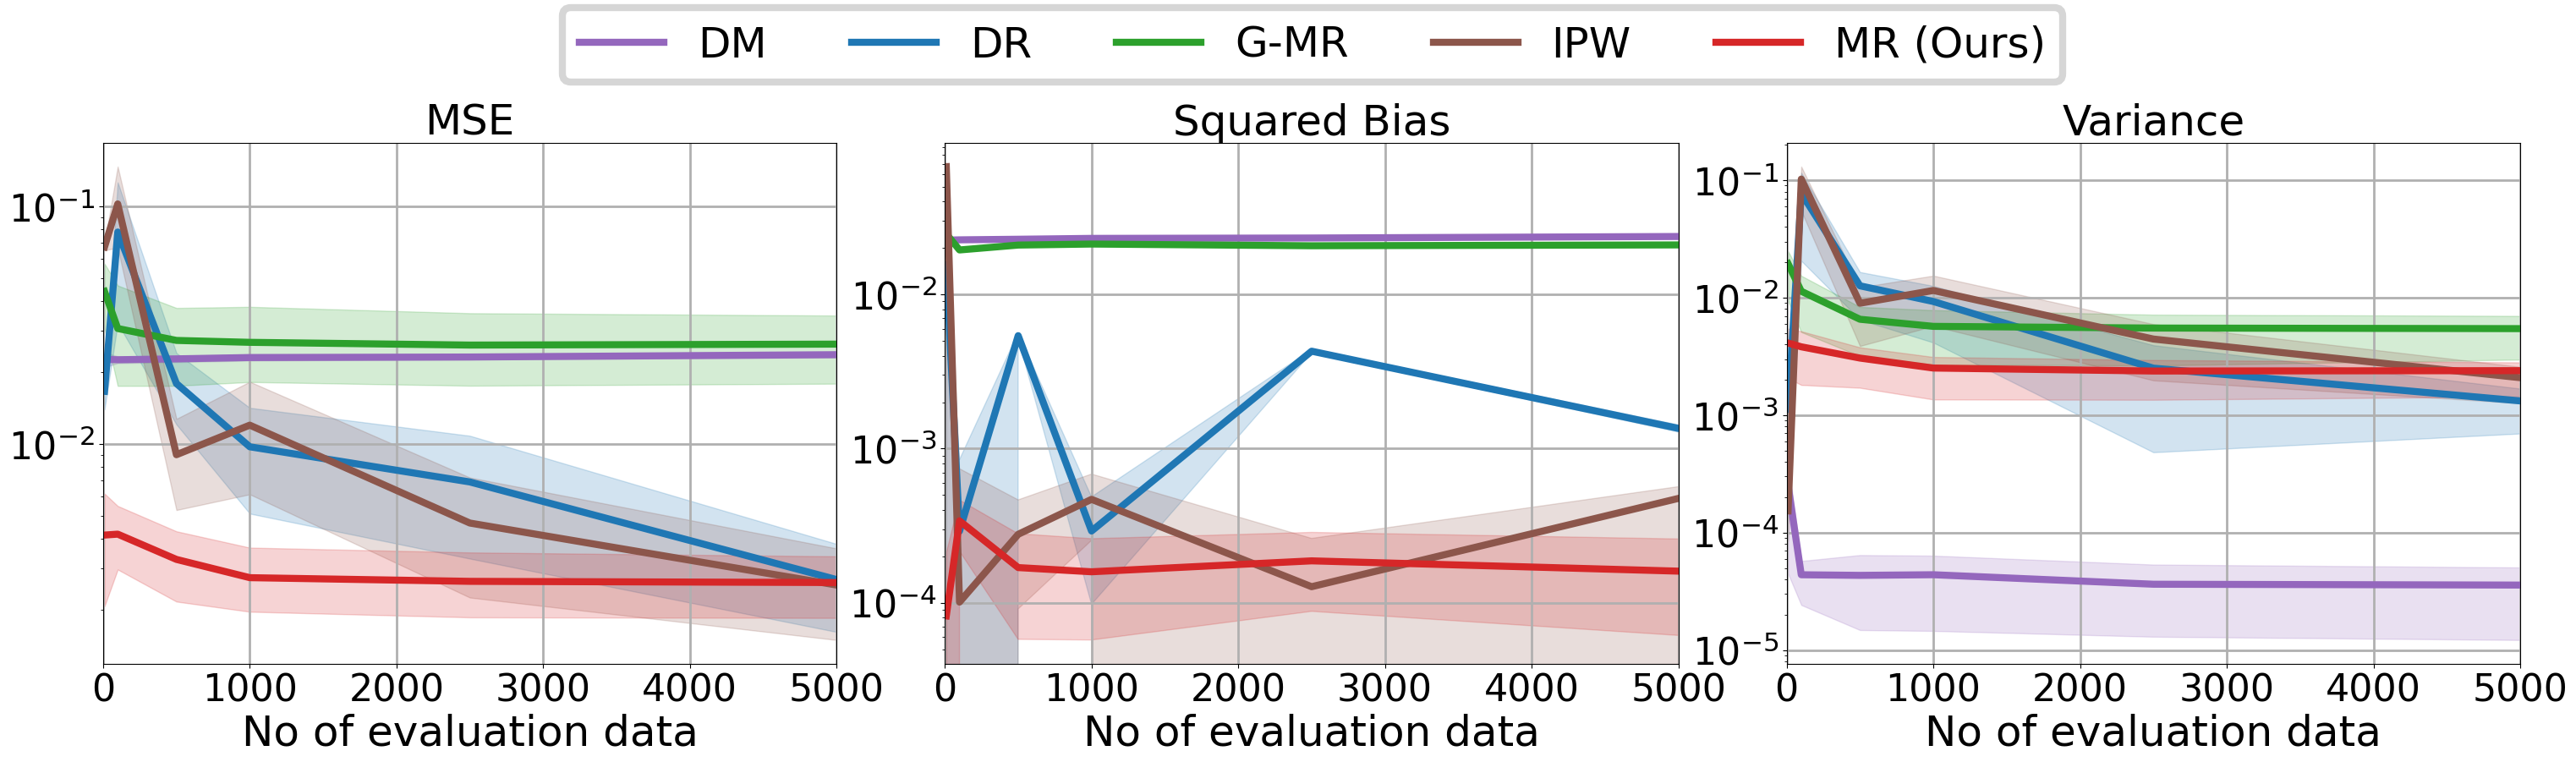
\includegraphics[width=0.75\textwidth]{figures/mr/ope_vs_neval_nac_100_alphatar_0_8_dimc_100_ntrain_100000.png}
%          \caption{Results with varying size of evaluation dataset $n$ for $\alpha^\ast = 0.8$.}
%          \label{fig:mse-vs-neval}
%      \end{subfigure}\\
%      \begin{subfigure}[b]{1\textwidth}
%          \centering
%          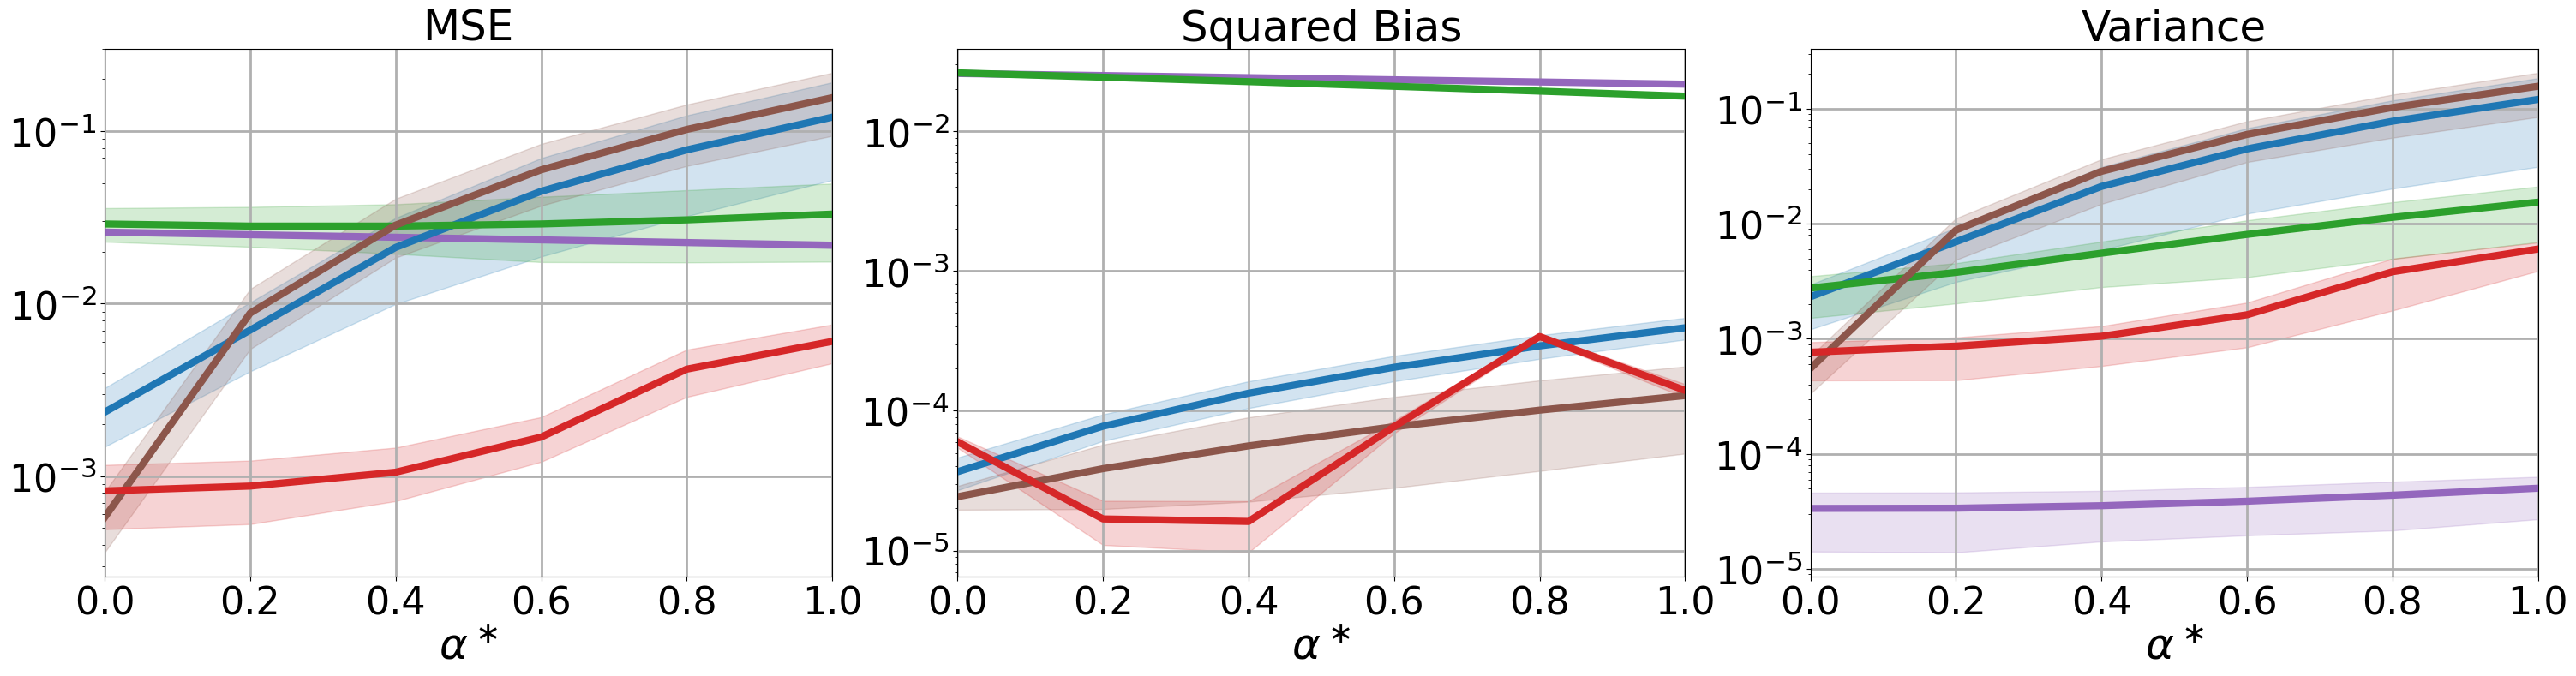
\includegraphics[width=0.75\textwidth]{figures/mr/ope_vs_alphatar_nac_100_neval_100_dimc_100_ntrain_100000.png}
%          \caption{Results with varying $\alpha^\ast$ for $n = 100$.}
%          \label{fig:mse-vs-betatar}
%      \end{subfigure}\\
%     \caption{Results with increasing $n$ and $\alpha^\ast$.}
%     \label{fig:syn_results1}
% \end{figure}
\myparagraph{Results}
We compute the target policy value using the $n$ evaluation datapoints. Here, the MSE of the estimators is computed over 10 different sets of logged data replicated with different seeds. The results presented have context dimension $d=1000$, number of actions $n_a=100$ and training data size $m=5000$. More experiments for a variety of parameter values are included in Appendix \ref{subsec:mips-empirical}.


% \begin{figure}
%      \centering
%      \begin{subfigure}[b]{1\textwidth}
%          \centering
%          \includegraphics[width=\textwidth]{figures/mr/latest/ope_vs_neval_nac_100_alphatar_0.2_dimc_100_ntrain_100000.png}
%          \caption{Results with varying size of evaluation dataset $n$ for $d=100$, $n_{a}=100$, $\alpha^\ast = 0.2$.}
%          \label{fig:mse-vs-neval}
%      \end{subfigure}\\
%      \begin{subfigure}[b]{1\textwidth}
%          \centering
%          \includegraphics[width=\textwidth]{figures/mr/latest/ope_vs_alphatar_dimc_100_nac_100_neval_100_ntrain_10000.png}
%          \caption{Results with varying $\alpha^\ast$ for $d=100$, $n_{a}=100$, $n = 100$.}
%          \label{fig:mse-vs-betatar}
%      \end{subfigure}\\
%      \begin{subfigure}[b]{1\textwidth}
%          \centering
%          \includegraphics[width=\textwidth]{figures/mr/latest/ope_vs_dimc_nac_100_alphatar_0.2_neval_100_ntrain_100000.png}
%          \caption{Results with varying context dimensions $d$ for $n_{a}=100$, $n = 100$, $\alpha^\ast = 0.2$.}
%          \label{fig:mse-vs-d}
%      \end{subfigure}\\
%      \begin{subfigure}[b]{1\textwidth}
%          \centering
%          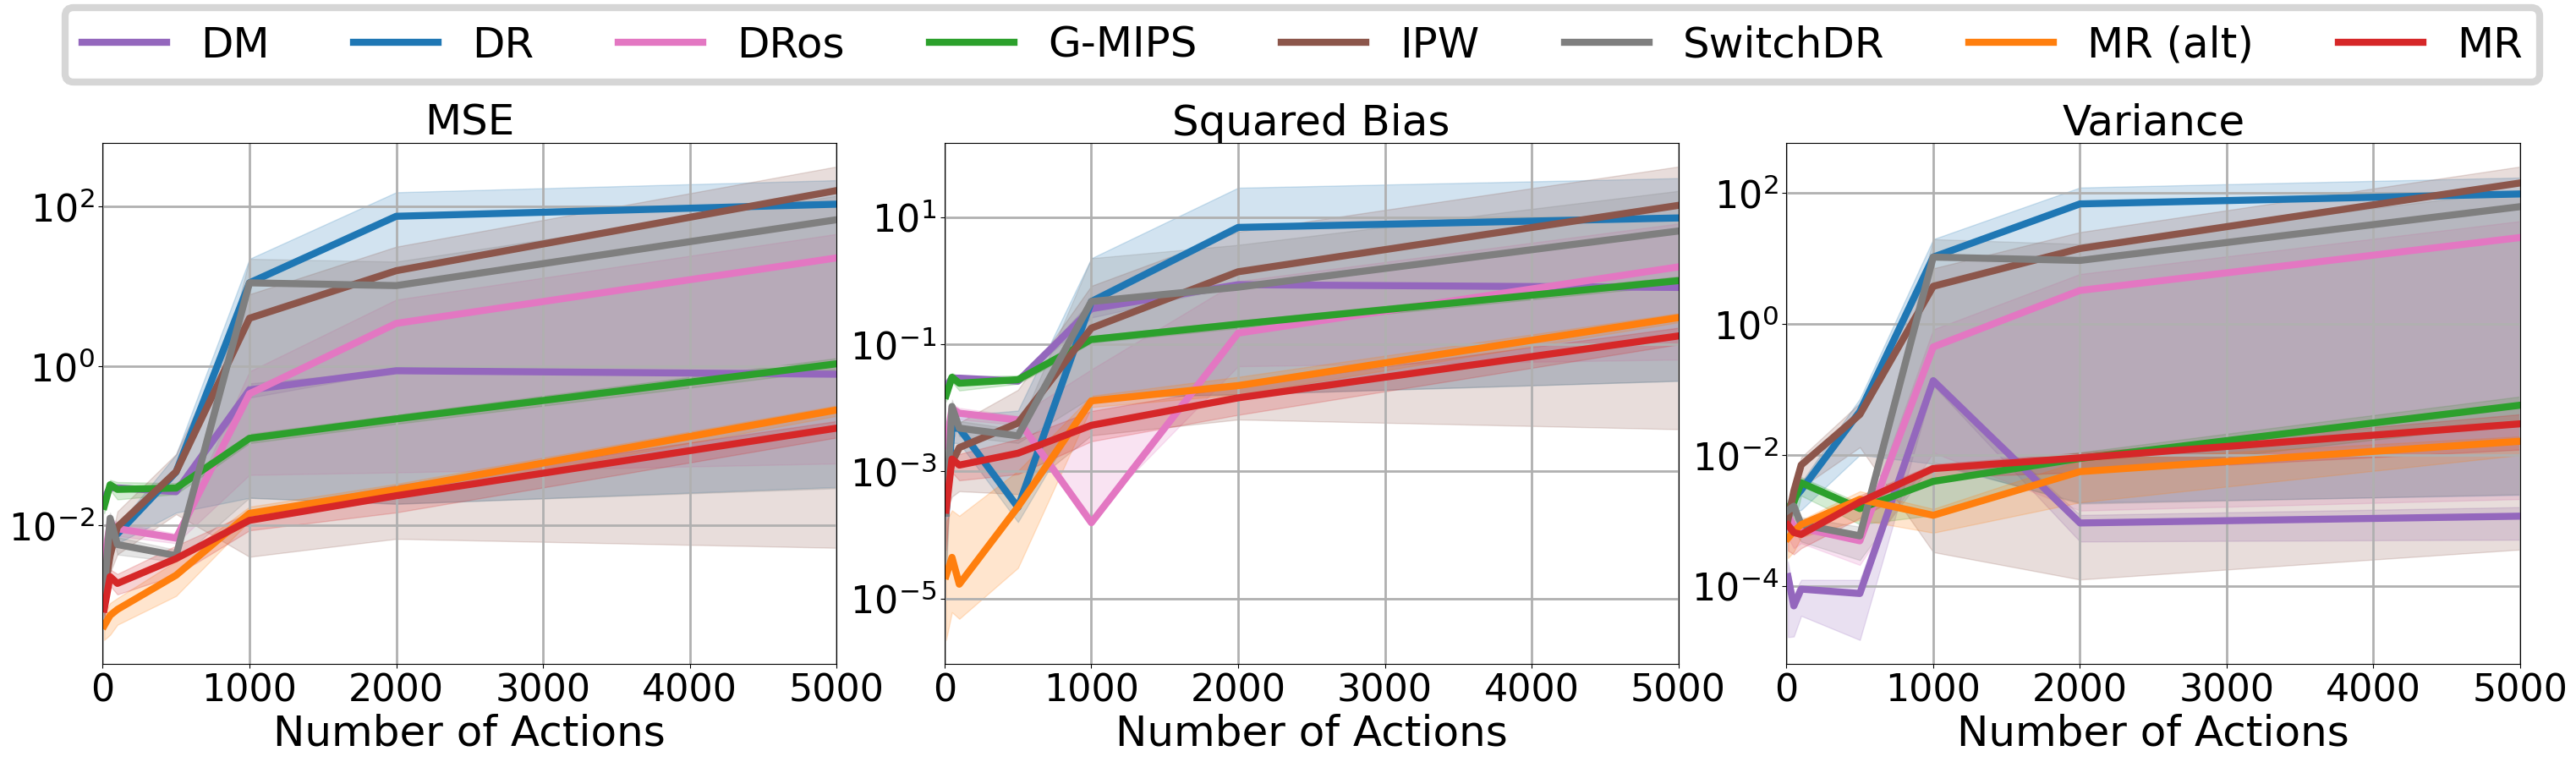
\includegraphics[width=\textwidth]{figures/mr/latest/ope_vs_nac_dimc_100_alphatar_0.2_neval_100_ntrain_100000.png}
%          \caption{Results with varying number of actions $n_{a}$ for $d=100$, $n = 100$, $\alpha^\ast = 0.2$.}
%          \label{fig:mse-vs-nac}
%      \end{subfigure}
%         \caption{Results for synthetic data experiments}
%         \label{fig:syn_results}
% \end{figure}

\myparagraph{Varying number of evaluation data $n$} 
In Figure \ref{fig:mse-vs-neval} we plot the results with increasing size of evaluation data $n$ increases. MR achieves the smallest MSE among all the baselines considered when $n$ is small, with the MSE of MR being at least an order of magnitude smaller than every baseline for $n\leq 500$. This shows that MR is significantly more accurate than the baselines when the size of the evaluation data is small. As $n\rightarrow \infty$, the difference between the results for MR and MIPS decreases. However, MR attains smaller variance and MSE than MIPS generally, verifying our analysis in Section \ref{subsec:mips-comparison}.
% IPW and DR become increasingly accurate because of their consistency and therefore the difference between MR and these baselines becomes less pronounced. 
% Additionally, it can be seen that the MR estimator also achieves the smallest squared bias overall. 
% In contrast, G-MR has a high squared bias as a result of the estimation error of the marginal ratio $\ptar(r)/\pbeh(r)$, which is more difficult to estimate the marginal ratio $\ptar(y)/\pbeh(y)$ as $r$ is two dimensional. The variance of G-MR estimator, on the other hand, is smaller than that of IPW when $n < 2000$, as suggested by Proposition \ref{prop:mips_var_reduction}.
Moreover, Figure \ref{fig:mse-vs-neval} shows that while the variance of MR is greater than that of DM, it still achieves the lowest MSE overall, owing to the high bias of DM.

\begin{wrapfigure}{r}{0.35\textwidth}
    \centering
    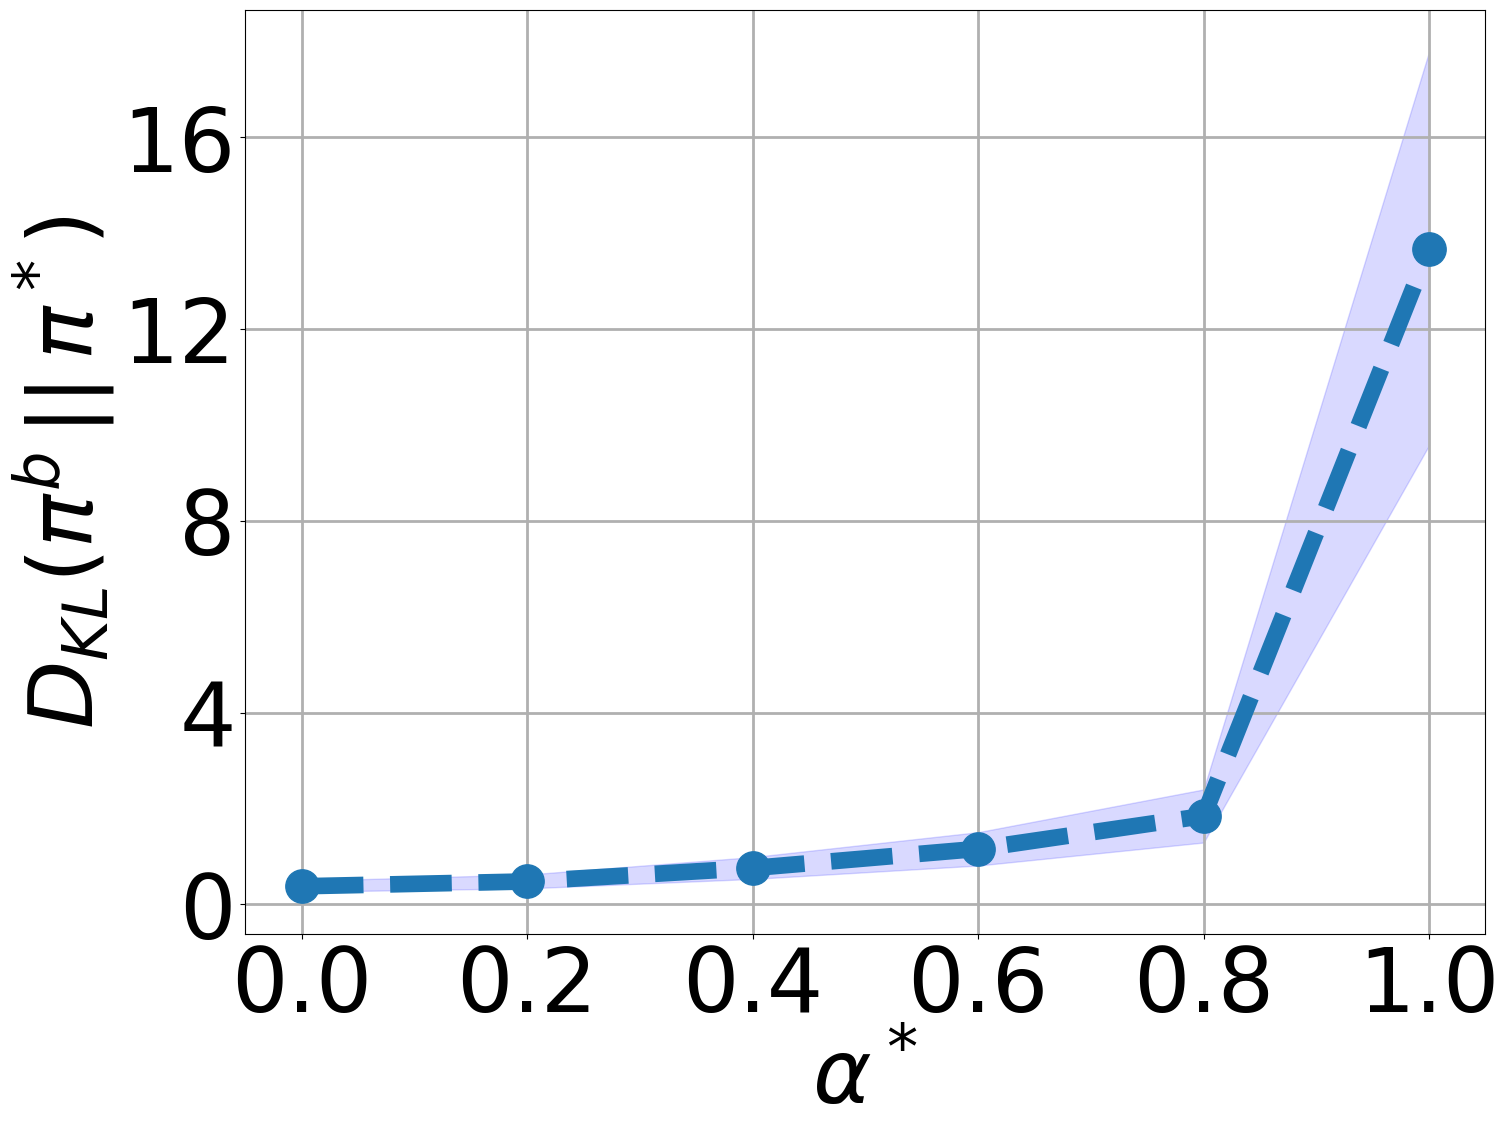
\includegraphics[width=0.35\textwidth]{figures/mr/kl-divergence-w-uncertainty.png}
    % \vspace{-0.75cm}
    % \caption{$D_{\textup{KL}}(\beh \,||\, \tar)$ with increasing $\alpha^\ast$}
    % \label{fig:kl-div-synthetic-data}
\end{wrapfigure}
\myparagraph{Varying $\alpha^\ast$}
As $\alpha^\ast$ parameter of the target policy increases, so does the shift between the policies $\beh$ and $\pi^{\alpha^\ast}$ as illustrated by the figure on the right, which plots the KL-divergence $D_{\textup{KL}}(\beh\, || \, \pi^{\alpha^\ast})$ as a function of $\alpha$.
% To analyse the shift between the policies $\beh$ and $\pi^{\alpha^\ast}$, the figure on the right plots the KL-divergence between the two policies as $\alpha^\ast$ increases. 
% \ref{fig:kl-div-synthetic-data}. 
% The figure shows that the shift between target and behaviour policies increases with increasing $\alpha^\ast$.
Figure \ref{fig:mse-vs-betatar} plots the results for increasing policy shift. 
Overall, the MSE of MR estimator is lowest among all the baselines. Moreover, while the MSE and variance of all estimators increase with increasing $\alpha^\ast$ the increase in these quantities is lower for the MR estimator than for the other baselines. Therefore, the relative performance of MR estimator improves with increasing policy shift and MR remains robust to increase in policy shift.
% It can be seen that the MSE of MR remains roughly the same with increasing $\alpha^\ast$, whereas the MSE of all other baselines increases. Moreover, both the squared bias and variance of the MR estimator becomes comparatively better than those of other baselines as the policy shift increases. 
% While the MSE and variances of all baselines increases with increasing $\beta^\ast$, the MSE and variance of MR estimator remains relatively small. Moreover, while the MSE of DM does not change noticeably with changing  $\beta^\ast$, it is still at least 2 orders of magnitude larger than that of MR. 
% This shows that MR remains significantly robust to increase in policy shift, relative to the other baselines.

\myparagraph{Additional ablation studies}
In Appendix \ref{subsec:mips-empirical}, we investigate the effect of varying context dimensions $d$, number of actions $n_a$ and number of training data $m$. In every case, we observe that the MR estimator has a smaller MSE than all other baselines considered. In particular, MR remains robust to increasing $n_a$ whereas the MSE and variance of IPW and DR estimators degrade substantially when $n_a \geq 2000$. Likewise, MR outperforms the baselines even when the training data size $m$ is small.

% \begin{figure}[t]
%      \centering
%      \begin{subfigure}[b]{0.5\textwidth}
%          \centering
%          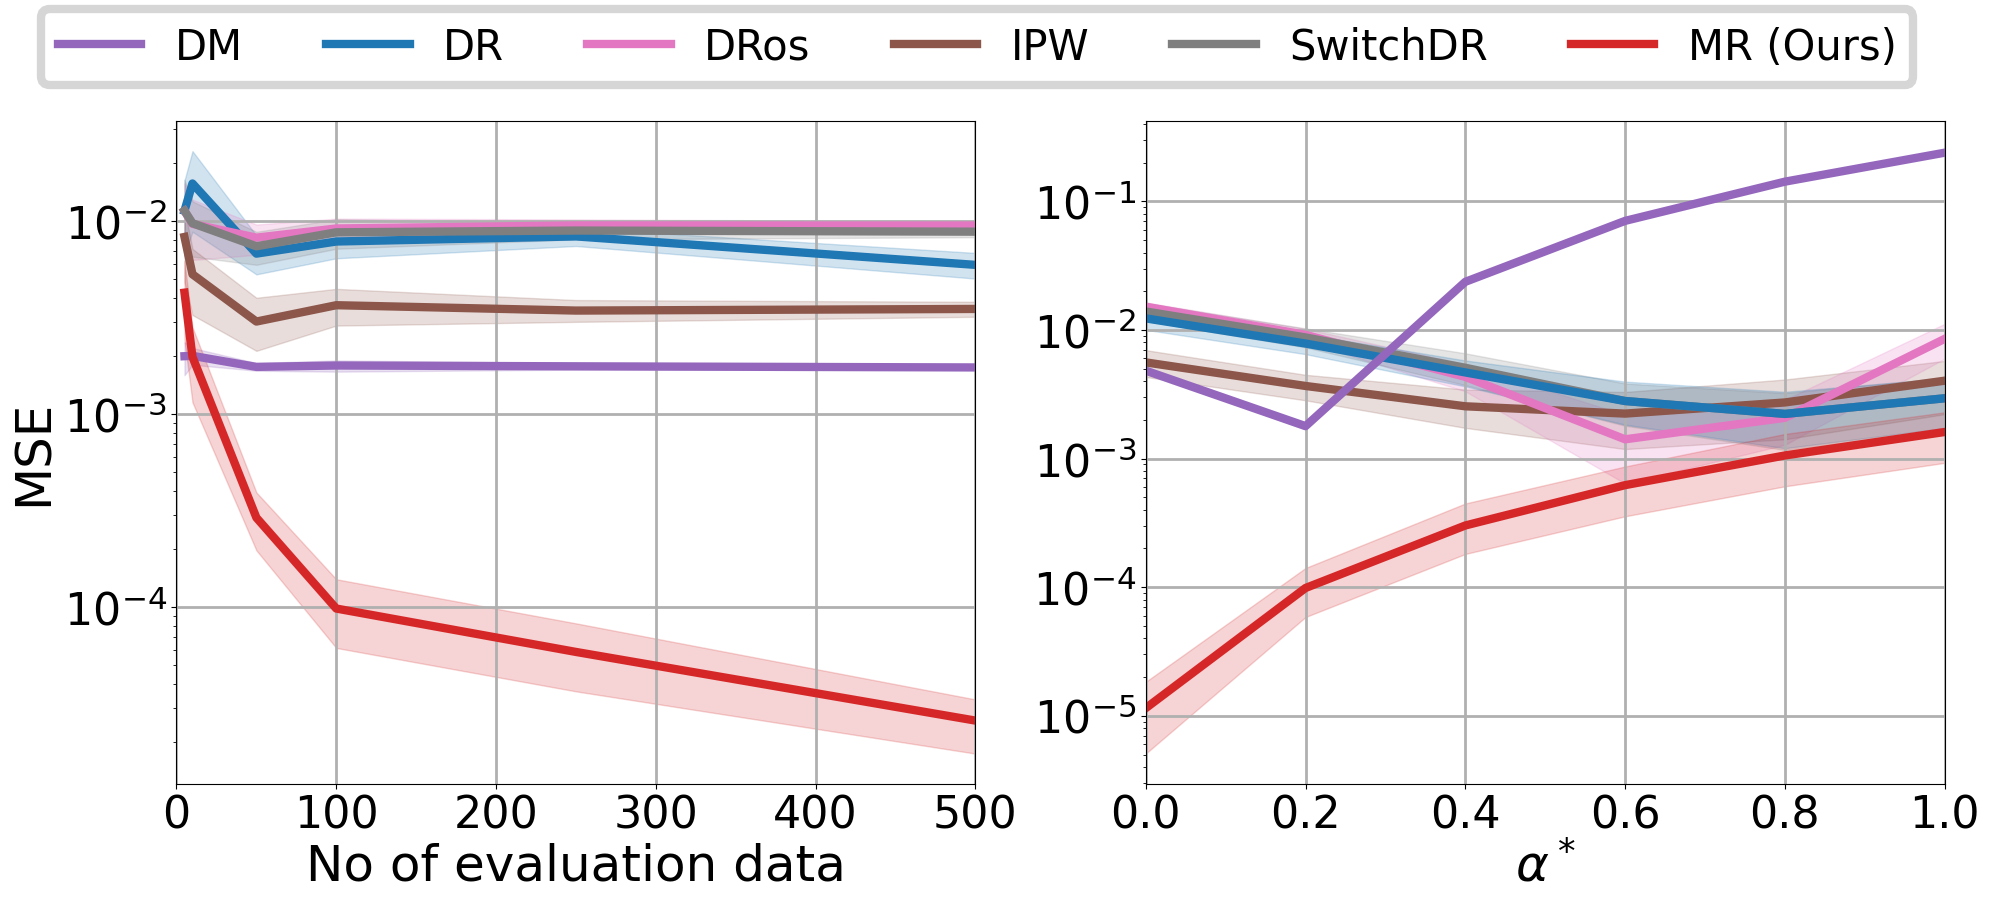
\includegraphics[height=0.92in]{figures/mr/pendigits_main.png}
%          \caption{Results for PenDigits dataset}
%          \label{fig:pendigits-main}
%      \end{subfigure}%
%      \begin{subfigure}[b]{0.5\textwidth}
%          \centering
%          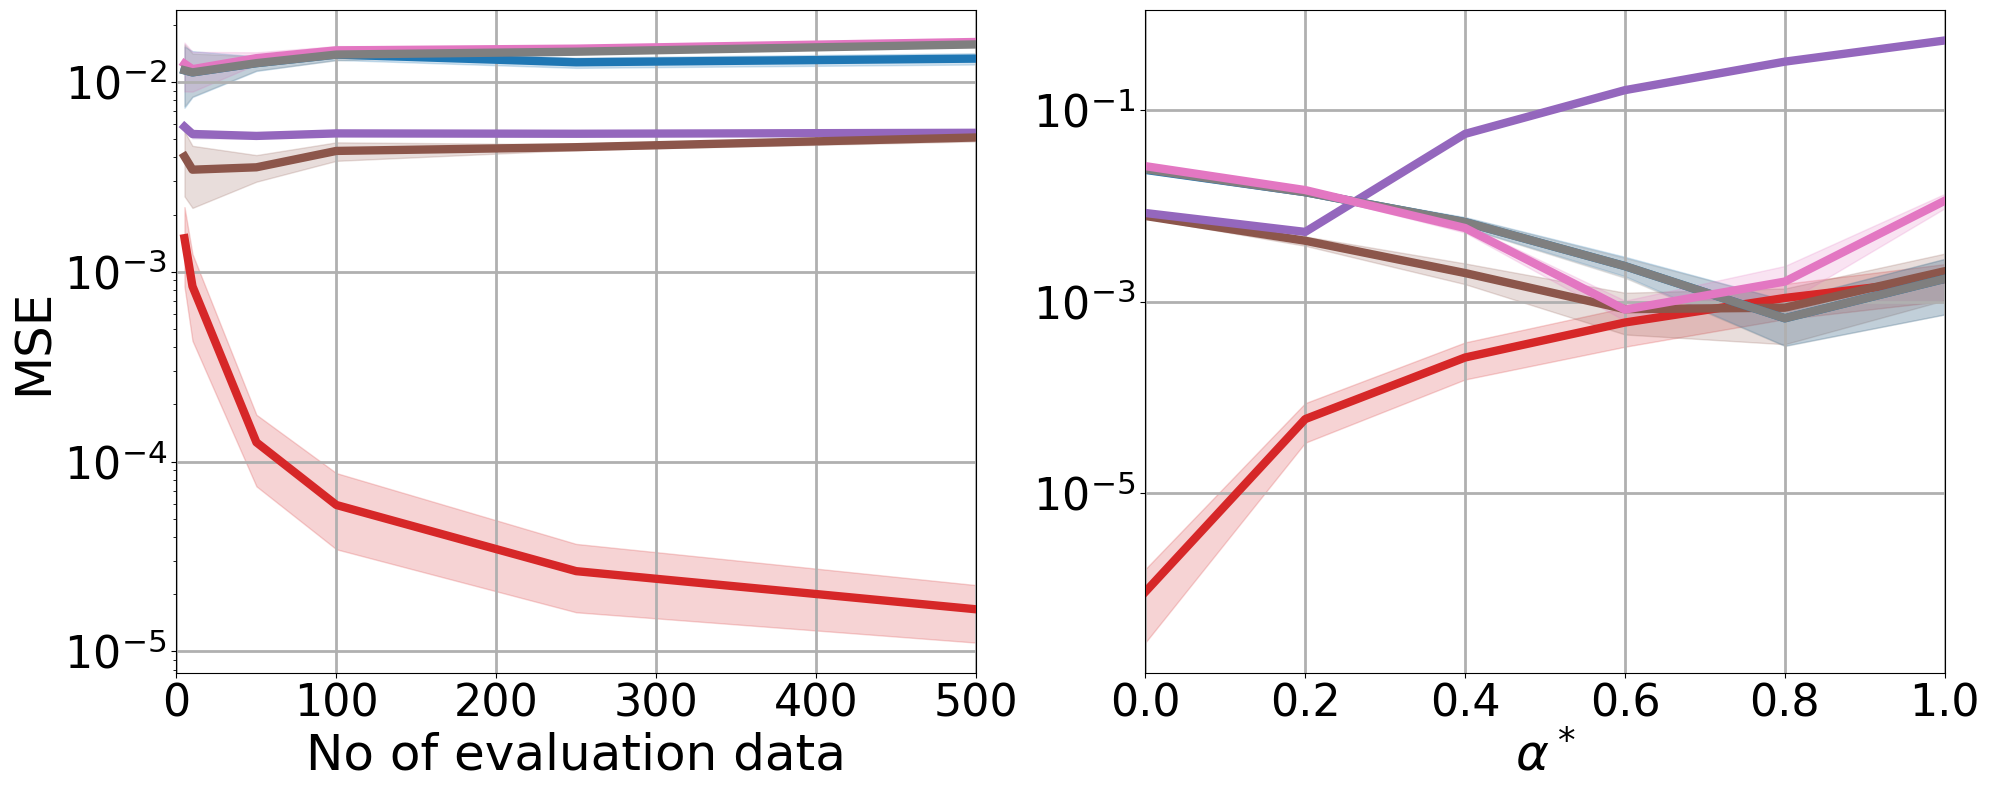
\includegraphics[height=0.92in]{figures/mr/mnist_main.png}
%          \caption{Results for mnist dataset.}
%          \label{fig:mnist-main}
%      \end{subfigure}\\
%     \caption{Results for synthetic data experiment. In \ref{fig:mse-vs-neval} we have $\alpha^\ast=0.8$ and in \ref{fig:mse-vs-betatar} we have $n = 100$.}
%     \label{fig:multiclass-main}
% \end{figure}
% \begin{table}[t]
%     \centering
%     \caption{Mean squared error of target policy value with standard errors over 10 different seeds for different classification datasets. Here, number of evaluation data $n=100$, and $\alpha^\ast=0.2$.}
%     \label{tab:classification-dataset-results}
%     \begin{tiny}
% \begin{tabular}{lllllll}
% \toprule
% Dataset & Digits & Letter & Mnist & OptDigits & PenDigits & SatImage \\
% \midrule
% DM & 0.00505$\pm$0.00016 & 0.01255$\pm$0.00011 & 0.00536$\pm$0.00009 & 0.00240$\pm$0.00009 & 0.00179$\pm$0.00011 & 0.00114$\pm$0.00005 \\
% DR & 0.01768$\pm$0.00058 & 0.00279$\pm$0.00093 & 0.01394$\pm$0.00084 & 0.00590$\pm$0.00089 & 0.00784$\pm$0.00128 & 0.02249$\pm$0.00660 \\
% DRos & 0.01721$\pm$0.00054 & 0.00281$\pm$0.00070 & 0.01467$\pm$0.00068 & 0.00788$\pm$0.00055 & 0.00916$\pm$0.00100 & 0.02160$\pm$0.00237 \\
% IPW & 0.00523$\pm$0.00030 & 0.00142$\pm$0.00062 & 0.00433$\pm$0.00044 & 0.00197$\pm$0.00035 & 0.00367$\pm$0.00077 & 0.01292$\pm$0.00455 \\
% SwitchDR & 0.01768$\pm$0.00058 & 0.00310$\pm$0.00087 & 0.01394$\pm$0.00084 & 0.00709$\pm$0.00054 & 0.00875$\pm$0.00135 & 0.02035$\pm$0.00289 \\
% MR (Ours) & \textbf{0.00011$\pm$0.00002} & \textbf{0.00020$\pm$0.00002} & \textbf{0.00006$\pm$0.00002} & \textbf{0.00025$\pm$0.00009} & \textbf{0.00010$\pm$0.00004} & \textbf{0.00014$\pm$0.00004} \\
% \bottomrule
% \end{tabular}
% \end{tiny}
% \end{table}
% \begin{table}[!htp]
%     \centering
%     \caption{Mean squared error of target policy value with standard errors over 10 different seeds for different classification datasets. Here, number of evaluation data $n=100$, and $\alpha^\ast=0.2$.}
%     \label{tab:classification-dataset-results}
%     \begin{tiny}
% \begin{tabular}{lllllll}
% \toprule
% Dataset & Digits & Letter & OptDigits & PenDigits & SatImage & Mnist \\
% \midrule
% DM & 0.00505$\pm$0.00016 & 0.01255$\pm$0.00011 & 0.00240$\pm$0.00009 & 0.00179$\pm$0.00011 & 0.00114$\pm$0.00005 & 0.00536$\pm$0.00009 \\
% DR & 0.01768$\pm$0.00058 & 0.00279$\pm$0.00093 & 0.00590$\pm$0.00089 & 0.00784$\pm$0.00128 & 0.02249$\pm$0.00660 & 0.01394$\pm$0.00084\\
% DRos & 0.01721$\pm$0.00054 & 0.00281$\pm$0.00070 & 0.00788$\pm$0.00055 & 0.00916$\pm$0.00100 & 0.02160$\pm$0.00237 & 0.01467$\pm$0.00068\\
% IPW & 0.00523$\pm$0.00030 & 0.00142$\pm$0.00062 & 0.00197$\pm$0.00035 & 0.00367$\pm$0.00077 & 0.01292$\pm$0.00455 & 0.00433$\pm$0.00044\\
% SwitchDR & 0.01768$\pm$0.00058 & 0.00310$\pm$0.00087 & 0.00709$\pm$0.00054 & 0.00875$\pm$0.00135 & 0.02035$\pm$0.00289 & 0.01394$\pm$0.00084\\
% MR (Ours) & \textbf{0.00011$\pm$0.00002} & \textbf{0.00020$\pm$0.00002} & \textbf{0.00025$\pm$0.00009} & \textbf{0.00010$\pm$0.00004} & \textbf{0.00014$\pm$0.00004} & \textbf{0.00006$\pm$0.00002}\\
% \bottomrule
% \end{tabular}
% \end{tiny}
% \end{table}
% \vspace{-5mm}
\begin{sidewaystable}[!htp]
    \centering
    \caption{Mean squared error of target policy value with standard errors over 10 different seeds for different classification datasets. Here, number of evaluation data $n=1000$, and $\alpha^\ast=0.6$.}
    \label{tab:classification-dataset-results}
    \begin{footnotesize}
    \begin{scshape}
% \begin{tabular}{lllllll}
% \toprule
% Dataset & Digits & Letter & OptDigits & PenDigits & SatImage & Mnist\\
% \midrule
% DM & 0.16053$\pm$0.00263 & 0.11686$\pm$0.00108 & 0.05963$\pm$0.00129 & 0.05889$\pm$0.00180 & 0.02165$\pm$0.00125 & 0.12556$\pm$0.00112 \\
% DR & 0.05694$\pm$0.00412 & 0.67369$\pm$0.31527 & 0.03697$\pm$0.00707 & 0.20803$\pm$0.13579 & 0.06484$\pm$0.04971 & 0.16665$\pm$0.01689 \\
% DRos & 0.03180$\pm$0.00231 & 0.05629$\pm$0.02057 & 0.00928$\pm$0.00181 & 0.00698$\pm$0.00236 & 0.00824$\pm$0.00212 & 0.06950$\pm$0.00549 \\
% IPW & 0.06465$\pm$0.00459 & 0.96803$\pm$0.44189 & 0.05451$\pm$0.00875 & 0.02769$\pm$0.00720 & 0.02298$\pm$0.00903 & 0.20363$\pm$0.02123 \\
% SwitchDR & 0.05694$\pm$0.00412 & 0.11881$\pm$0.02220 & 0.04086$\pm$0.00711 & 0.02150$\pm$0.00569 & 0.01677$\pm$0.00598 & 0.16665$\pm$0.01689 \\
% MR (Ours) & \textbf{0.00169$\pm$0.00032} & \textbf{0.00126$\pm$0.00045} & \textbf{0.00115$\pm$0.00040} & \textbf{0.00261$\pm$0.00062} & \textbf{0.00314$\pm$0.00071} & \textbf{0.00654$\pm$0.00092} \\
% \bottomrule
% \end{tabular}

\begin{tabular}{llllllll}
\toprule
Dataset &             Digits &               Letter &          OptDigits &          PenDigits &           SatImage  &              Mnist & CIFAR-100\\
\midrule
DM        &  0.1508$\pm$0.0015 &    0.0886$\pm$0.0026 &  0.0485$\pm$0.0016 &   0.0520$\pm$0.0016 &  0.0208$\pm$0.0009  &  0.1109$\pm$0.0014 & 0.0020$\pm$0.0001 \\
DR        &    0.1334$\pm$0.0400 &    \red{35.085$\pm$17.768} &  0.0464$\pm$0.0061 &  0.2343$\pm$0.1404 &   0.0560$\pm$0.0395 &  0.2617$\pm$0.0139 & \red{3823.9$\pm$2023.2} \\
DRos      &  0.0847$\pm$0.0025 &    0.2363$\pm$0.0586 &  0.0384$\pm$0.0025 &  0.0138$\pm$0.0029 &  0.0078$\pm$0.0008 &  0.2151$\pm$0.0061 & 0.2628$\pm$0.1087 \\
IPW       &  0.1632$\pm$0.0462 &  \red{45.253$\pm$22.057} &   0.0844$\pm$0.0056 &  0.1342$\pm$0.0531 &    0.0900$\pm$0.0676 & 0.3359$\pm$0.0118 & \red{4116.9$\pm$2097.9}\\
SwitchDR  &  0.0982$\pm$0.0032 &    0.2387$\pm$0.0507 &  0.0557$\pm$0.0047 &   0.0342$\pm$0.0090 &  0.0136$\pm$0.0012  &   0.2750$\pm$0.0102 & 1.1644$\pm$0.8227 \\
MR (Ours) &  \textbf{0.0034$\pm$0.0001} &    \textbf{0.0018$\pm$0.0004} &  \textbf{0.0006$\pm$0.0002} &  \textbf{0.0008$\pm$0.0002} &  \textbf{0.0016$\pm$0.0003} &  \textbf{0.0121$\pm$0.0009} &  \textbf{0.0007$\pm$0.0002}\\
\bottomrule
\end{tabular}

% \begin{tabular}{lllllll}
% \toprule
% Dataset & Digits & Letter & OptDigits & PenDigits & SatImage & Mnist\\
% \midrule
% DM & 0.161$\pm$0.003 & 0.117$\pm$0.001 & 0.060$\pm$0.001 & 0.059$\pm$0.002 & 0.022$\pm$0.001 & 0.126$\pm$0.001 \\
% DR & 0.057$\pm$0.004 & 0.674$\pm$0.315 & 0.037$\pm$0.007 & 0.208$\pm$0.136 & 0.065$\pm$0.050 & 0.167$\pm$0.017 \\
% DRos & 0.032$\pm$0.002 & 0.056$\pm$0.021 & 0.009$\pm$0.002 & 0.007$\pm$0.002 & 0.008$\pm$0.002 & 0.070$\pm$0.005 \\
% IPW & 0.065$\pm$0.005 & 0.968$\pm$0.442 & 0.055$\pm$0.009 & 0.028$\pm$0.007 & 0.023$\pm$0.009 & 0.204$\pm$0.021 \\
% SwitchDR & 0.057$\pm$0.004 & 0.118$\pm$0.022 & 0.041$\pm$0.007 & 0.022$\pm$0.006 & 0.017$\pm$0.006 & 0.167$\pm$0.017 \\
% MR (Ours) & \textbf{0.002$\pm$0.001} & \textbf{0.001$\pm$0.001} & \textbf{0.001$\pm$0.001} & \textbf{0.003$\pm$0.001} & \textbf{0.003$\pm$0.001} & \textbf{0.007$\pm$0.001} \\
% \bottomrule
% \end{tabular}
\end{scshape}
\end{footnotesize}
\end{sidewaystable}
\subsection{Experiments on classification datasets}
Following previous works on OPE in contextual bandits \citep{dudik2014doubly, kallus2021optimal, mehrdad2018more,wang2017optimal}, we transform classification datasets into contextual bandit feedback data in this experiment.
We consider five UCI classification datasets \citep{dua2019uci} as well as Mnist \citep{deng2012mnist} and CIFAR-100 \citep{krizhevsky2009learning} datasets, each of which comprises $\{(x_i, a^\gt_i)\}_{i}$, where $x_i\in \Xspace$ are feature vectors and $a^\gt_i\in \Aspace$ are the ground-truth labels.
% Here, the datasets considered include five UCI classification datasets \citep{dua2019uci}, as well as the mnist dataset \citep{deng2012mnist}. 
% Following previous works \citep{dudik2014doubly, kallus2021optimal, mehrdad2018more,wang2017optimal}, the classification datasets are transformed to contextual bandit feedback data. 
In the contextual bandits setup, the feature vectors $x_i$ are considered to be the contexts, whereas the actions correspond to the possible class of labels. For the context vector $x_i$ and the action $a_i$, the reward $y_i$ is defined as $y_i \coloneqq \ind(a_i = a^\gt_i)$, i.e., the reward is 1 when the action is the same as the ground truth label and 0 otherwise. Here, the baselines considered include the DM, IPW and DR estimators as well as Switch-DR \citep{wang2017optimal} and DR with Optimistic Shrinkage (DRos) \citep{su2020doubly}. We do not consider a MIPS baseline here as there is no natural embedding $E$ of $A$. Additional details are provided in Appendix \ref{subsec:additional-experiments-classification}. 
% regarding the behaviour and target policies and the estimation of weights are provided in Appendix \ref{sec:app-additional-results}. 
% Similar to the synthetic data experiments, we define a class of parametric target policies parameterised by $\alpha^\ast \in [0, 1]$ (i.e., $\tar = \pi^{\alpha^\ast}$). 
% However, we show in Appendix \ref{subsec:additional-experiments} that in this case, the shift between target and behaviour policies increases as $\alpha^\ast \rightarrow 0$.

In Table \ref{tab:classification-dataset-results}, we present the results with number of evaluation data $n=1000$ and number of training data $m=500$. 
The table shows that across all datasets, MR achieves the lowest MSE among all methods. \flag{Moreover, for the Letter and CIFAR-100 datasets the IPW and DR yield large bias and variance arising from poor policy estimates $\hatbeh$. Despite this, the MR estimator which utilizes the \emph{same} $\hatbeh$ for the estimation of $\hat{w}(y)$ leads to much more accurate results.} We also verify that MR outperforms the baselines for increasing policy shift and evaluation data $n$ in Appendix \ref{subsec:additional-experiments-classification}.
% In fact, the MSE of MR is at least an order of magnitude lower than that of other methods.


% We provide extensive results for increasing policy shift and evaluation data size $n$ in Appendix \ref{sec:app-additional-results}.

% We split the dataset into training and testing datasets of sizes $m$ and $n$ respectively.

% \paragraph{Reward function}
% Let $X$ be a context with ground truth label $A^\gt$, we define the reward for action $A$ as:
% \[
% Y \coloneqq \ind(A = A^\gt).
% \]

\subsection{Application to ATE estimation}\label{subsec:causal-experiments}
% Further to our discussion regarding the application of MR for ATE estimation in Section \ref{subsec:application-to-causal-inference}, 
In this experiment, we investigate the empirical performance of the MR estimator for ATE estimation. 

\myparagraph{Twins dataset}
We use the Twins dataset studied in \cite{louizos2017causal}, which comprises data from twin births in the USA between 1989-1991. The treatment $a=1$ corresponds to being born the heavier twin and the outcome $Y$ corresponds to the mortality of each of the twins in their first year of life. Specifically, $Y(1)$ corresponds to the mortality of the heavier twin (and likewise for $Y(0)$). To simulate the observational study, we follow a similar strategy as in \cite{louizos2017causal} to selectively hide one of the two twins as explained in Appendix \ref{app:ate-empirical}. We obtain a total of 11,984 datapoints, of which 5000 datapoints are used to train the behaviour policy $\hatbeh$ and outcome model $\hat{q}(x, a)$.

% Here, the baselines considered include the DM, IPW and DR estimators as well as Switch-DR \citep{wang2017optimal} and DR with Optimistic Shrinkage (DRos) \citep{su2020doubly}. We do not consider a MIPS baseline here as there is no natural embedding $E$ of $A$. 
% Results for additional baselines have been given in Appendix \ref{app:ate-empirical}. 

% \begin{wraptable}{l}{0.55\textwidth}
\begin{table}[t]
% \vspace{-4mm}
    \centering
    \caption{Mean absolute ATE estimation error $\epsilon_\ate$ with standard errors over 10 different seeds, for increasing number of evaluation data $n$.}
    \label{tab:ate_errors-main}
    \begin{small}
    \begin{tabular}{lllll}
\toprule
$n$ &             50   &             200  &             1600 &             3200 \\
\midrule
DM       &  0.092$\pm$0.003 &  0.092$\pm$0.003 &  0.092$\pm$0.004 &  0.092$\pm$0.004 \\
DR       &  0.101$\pm$0.024 &  \textbf{0.065$\pm$0.009} &  0.071$\pm$0.005 &  0.069$\pm$0.004 \\
\textsc{DRos}     &    0.100$\pm$0.017 &  0.089$\pm$0.006 &   0.093$\pm$0.004 &  0.087$\pm$0.004 \\
IPW      &  0.092$\pm$0.024 &  0.088$\pm$0.014 &  0.067$\pm$0.007 &  0.067$\pm$0.007 \\
\textsc{SwitchDR} &  0.101$\pm$0.024 &  \textbf{0.065$\pm$0.009} &  0.071$\pm$0.005 &  0.069$\pm$0.004 \\
MR (Ours)      &  \textbf{0.062$\pm$0.007} &  \textbf{0.065$\pm$0.007} &  \textbf{0.061$\pm$0.005} &  \textbf{0.061$\pm$0.006} \\
\bottomrule
\end{tabular}
\end{small}
% \vspace{-4mm}
\end{table}
% \end{wraptable}
Here, we consider the same baselines as the classification data experiments in previous section.
For our evaluation, we consider the absolute error in ATE estimation, $\epsilon_\ate$, defined as:
$
\epsilon_\ate \coloneqq | \hat{\theta}^{(n)}_\ate - \theta_\ate |.
$
Here, $\hat{\theta}^{(n)}_\ate$ denotes the value of the ATE estimated using $n$ evaluation datapoints.
%\subsubsection{Results}
We compute the ATE value using the $n$ evaluation datapoints, over 10 different sets of observational data (using different seeds). Table \ref{tab:ate_errors-main} shows that MR achieves the lowest estimation error $\epsilon_\ate$ for all values of $n$ considered here. While the performance of other baselines improves with increasing $n$, MR outperforms them all. 
% Unlike other baselines, MR uses all datapoints to estimate $\E[Y(a)]$ for $a\in \{0, 1\}$ and consequently is more data efficient. 


% \begin{figure}[t]
%      \centering
%      \begin{subfigure}[b]{1\textwidth}
%          \centering
%          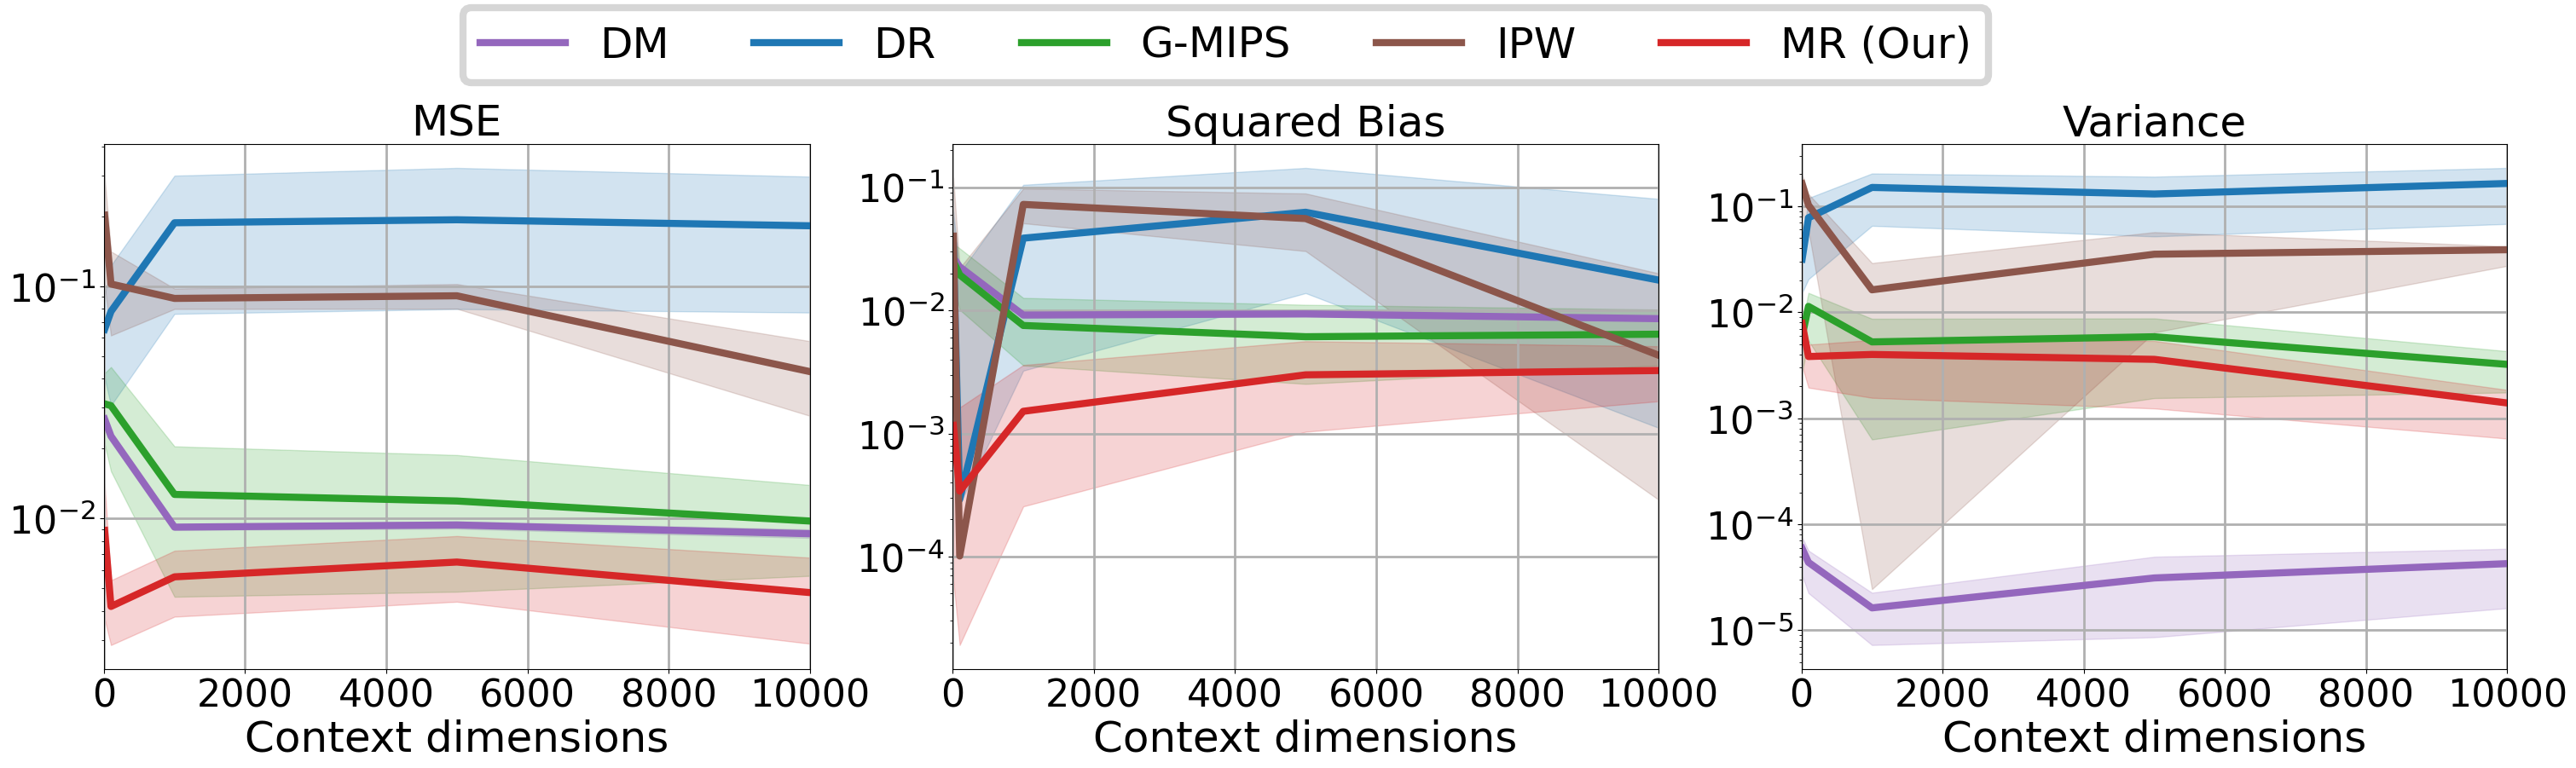
\includegraphics[width=0.75\textwidth]{figures/mr/ope_vs_dimc_nac_100_alphatar_0_8_neval_100_ntrain_100000.png}
%          \caption{Results with varying context dimensions $d$ for $n_{a}=100$, $n = 100$, $\alpha^\ast = 0.8$.}
%          \label{fig:mse-vs-d}
%      \end{subfigure}\\
%      \begin{subfigure}[b]{1\textwidth}
%          \centering
%          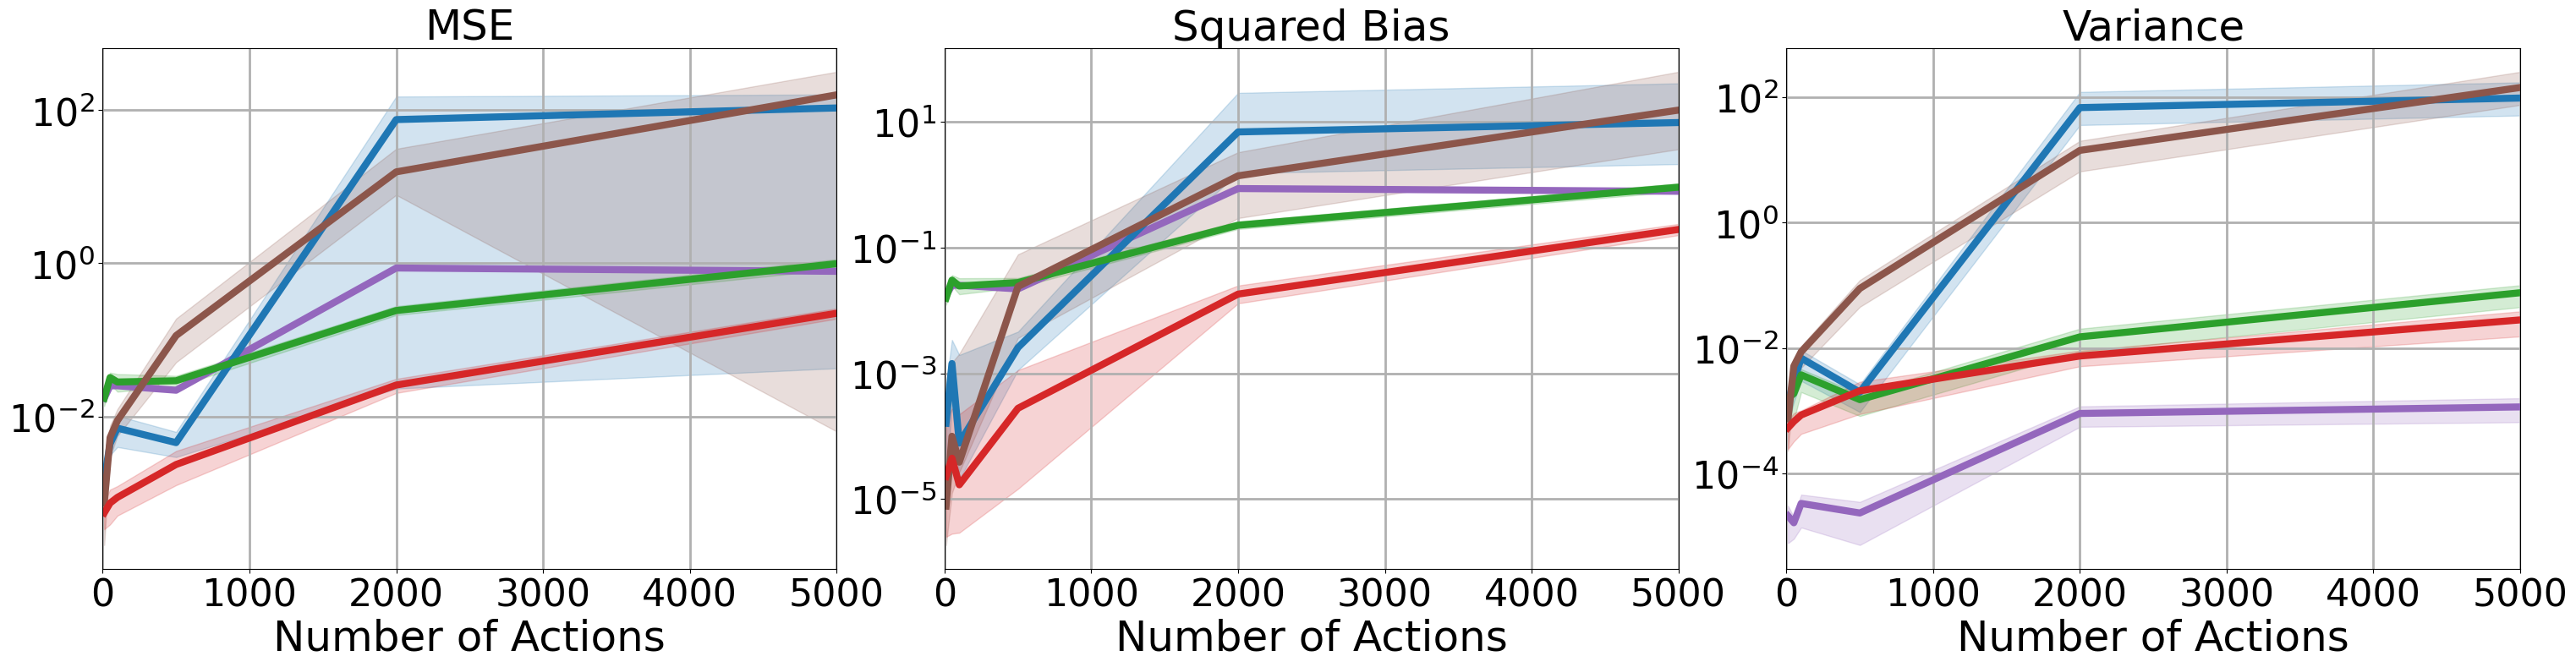
\includegraphics[width=0.75\textwidth]{figures/mr/ope_vs_nac_dimc_100_alphatar_0_2_neval_100_ntrain_100000.png}
%          \caption{Results with varying number of actions $n_{a}$ for $d=100$, $n = 100$, $\alpha^\ast = 0.2$.}
%          \label{fig:mse-vs-nac}
%      \end{subfigure}
%         \caption{Results with increasing $d$ and $n_a$.}
%         \label{fig:syn_results2}
% \end{figure}
% \paragraph{Varying $d$}
% Figure \ref{fig:mse-vs-d} plots how the results for different estimators changes as the context dimensions $d$ increases. While the results for the different baselines do not change significantly with increasing $d$, overall the MSE of MR estimator is smaller than that of other baselines.


% \paragraph{Varying $n_a$}
% Figure \ref{fig:mse-vs-nac} plots how the performance of different estimators changes as the number of actions $n_a$ increases. 
% It can be seen that the MSE and variance of IPW and DR estimators explodes when $n_a \geq 2000$. This happens because the variance of the policy ratios $\rho(a, x)$ is very large for large action spaces. In contrast, the MSE and variances of MR estimator remains relatively small even when $n_a$ is large. This shows that MR remains significantly robust in large action spaces. 

% Again, the MSE of MR estimator remains significantly smaller than the baselines with increasing values of $n_a$.
% \faaiz{think about plotting results versus the variance of policy ratios $\rho(x, a)$.}

\section{Discussion}
% \begin{itemize}
%     \item In this paper, we present marginal ratio estimator (MR) for off-policy evaluation which only considers the shift in the marginal distribution of the rewards resulting from the policy shift.
%     \item We show, theoretically and empirically, that the proposed method achieves better variance and MSE than the current SOTA methods, and is more data efficient overall.
%     \item We also show that our proposal can be used in the setting of causal inference, and provides more accurate results than the most commonly used methods.
% \end{itemize}

In this paper, we proposed an OPE method for contextual bandits called marginal ratio (MR) estimator, which considers only the shift in the marginal distribution of the outcomes resulting from the policy shift. Our theoretical and empirical analysis showed that MR achieves better variance and MSE compared to the current state-of-the-art methods and is more data efficient overall. Additionally, we demonstrated that MR applied to ATE estimation provides more accurate results than most commonly used methods. Next, we discuss limitations of our methodology and possible avenues for future work.

\myparagraph{Limitations}
The MR estimator requires the additional step of estimating $\hat{w}(y)$ which may introduce an additional source of bias in the value estimation. However, $\hat{w}(y)$ can be estimated by solving a simple 1d regression problem, and as we show empirically in Appendix \ref{app:experiments}, MR achieves the smallest bias among all baselines considered in most cases. Most notably, our ablation study in Appendix \ref{subsec:mips-empirical} shows that even when the training data is reasonably small, MR outperforms the baselines considered. 
% When the behaviour policy $\beh$ is unknown, MR estimator requires the splitting of training data to first estimate $\beh$ and subsequently to use this to estimate marginal weights $w(y)$. This data splitting can be costly in low-data settings, where we do not have access to large training datasets. However, as we empirically show in Appendix \ref{subsec:additional-experiments}, even when the training data is small, MR outperforms the baselines.  


\myparagraph{Future work}
The MR estimator can also be applied to policy optimisation problems, where the data collected using an `old' policy is used to learn a new policy. This approach has been used in Proximal Policy Optimisation (PPO) \citep{schulman2017proximal} for example, which has gained immense popularity and has been applied to reinforcement learning with human feedback (RLHF) \citep{lambert2022illustrating}. We believe that the MR estimator applied to these methodologies could lead to improvements in the stability and convergence of these optimisation schemes, given its favourable variance properties.


% \section*{Acknowledgements}
We would like to thank Jake Fawkes, Siu Lun Chau, Shahine Bouabid and Robert Hu for their useful feedback. 
We also appreciate the insights and constructive criticisms provided by the anonymous reviewers.
MFT acknowledges his PhD funding from Google DeepMind.

\clearpage

\chapter{\label{ch:4-copp}Conformal Off-Policy Prediction in Contextual Bandits} 

\minitoc
% 
% \usepackage[utf8]{inputenc} % allow utf-8 input
% \usepackage[T1]{fontenc}    % use 8-bit T1 fonts
% \usepackage[hidelinks]{hyperref}% hyperlinks
% \usepackage{url}            % simple URL typesetting
% \usepackage{booktabs}       % professional-quality tables
% \usepackage{amsfonts}       % blackboard math symbols
% \usepackage{nicefrac}       % compact symbols for 1/2, etc.
% \usepackage{microtype}      % microtypography
% \usepackage{xcolor}         % colors

% \usepackage{lipsum}

% \newcommand\blfootnote[1]{%
%   \begingroup
%   \renewcommand\thefootnote{}\footnote{#1}%
%   \addtocounter{footnote}{-1}%
%   \endgroup
% }



% \title{Conformal Off-Policy Prediction in Contextual Bandits}


% The \author macro works with any number of authors. There are two commands
% used to separate the names and addresses of multiple authors: \And and \AND.
%
% Using \And between authors leaves it to LaTeX to determine where to break the
% lines. Using \AND forces a line break at that point. So, if LaTeX puts 3 of 4
% authors names on the first line, and the last on the second line, try using
% \AND instead of \And before the third author name.

% \author[1]{Muhammad Faaiz Taufiq*} 
% \author[2]{Jean-Fran\c cois Ton*} 
% \author[1]{Rob Cornish} 
% \author[1]{Yee Whye Teh} 
% \author[1]{Arnaud Doucet} 

% \affil[1]{Department of Statistics, University of Oxford}
% \affil[2]{ByteDance Research}

% \author{%
%   Muhammad Faaiz Taufiq* \\
%   Department of Statistics\\
%   University of Oxford\\
%   % examples of more authors
%    \And
%    Jean-Francois Ton*$^\dagger$ \\
%    AI-Lab-Research\\
%    Bytedance AI Lab \\
%    \AND
%    Rob Cornish \\
%    Department of Statistics \\
%    University of Oxford\\
%    \And
%    Yee Whye Teh \\
%    Department of Statistics \\
%    University of Oxford\\
%    \And
%    Arnaud Doucet \\
%    Department of Statistics \\
%    University of Oxford\\
% }



\begin{abstract}
  Most off-policy evaluation methods for contextual bandits have focused on the expected outcome of a policy, which is estimated via methods that at best provide only asymptotic guarantees. However, in many applications, the expectation may not be the best measure of performance as it does not capture the variability of the outcome. In addition, particularly in safety-critical settings, stronger guarantees than asymptotic correctness may be required. To address these limitations, we consider a novel application of conformal prediction to contextual bandits. Given data collected under a behavioral policy, we propose \emph{conformal off-policy prediction} (COPP), which can output reliable predictive intervals for the outcome under a new target policy. We provide theoretical finite-sample guarantees without making any additional assumptions beyond the standard contextual bandit setup, and empirically demonstrate the utility of COPP compared with existing methods on synthetic and real-world data. 
  % \blfootnote{$^*$Denotes equal contribution, where ordering was determined through coin flip. Corresponding authors \texttt{muhammad.taufiq@stats.ox.ac.uk} and \texttt{jeanfrancois@bytedance.com}.
%   \blfootnote{$\dagger$ Work primarily done at the University of Oxford and finished at Bytedance.}
\end{abstract}

\section{Introduction}
% Often in safety-critical environments such as healthcare, we cannot afford to implement new policies, without reliably evaluating the effectiveness/safety of the policies. In such situations, we must resort to using available observational data to infer outcomes under a new target policy which has not been implemented in the real world. This is known as off-policy evaluation. 


% \R{In domains such as healthcare or recommendation systems, understanding all the possible outcomes is at the core of safe and informed decision making.} Due to ethical or financial constraints, we can often not implement new policies $\pi^*$, without first reliably evaluating its effectiveness and safety. In such cases we have to rely on observational data, which has been collected under a different policy $\pi^b$. Using this data to evaluate a policy $\pi^*$ is known as off-policy evaluation (OPE) and helps us assess $\pi^*$ without having to deploy it.
% % which can be both costly and risky. we use the same formulationas in Romano et al. (2019), i.
% % Hence it is crucial to determine the most likely outcomes under a new policy in a reliable manner.


Before deploying a decision-making policy to production, it is usually important to understand the plausible range of outcomes that it may produce.
However, due to resource or ethical constraints, it is often not possible to obtain this understanding by testing the policy directly in the real-world.
In such cases we have to rely on observational data collected under a different policy than the target.
Using this observational data to evaluate the target policy is known as off-policy evaluation (OPE).% and helps us assess $\pi^*$ without having to deploy it.


% policies $\pi^*$, without first reliably evaluating its effectiveness and safety. In such cases we have to rely on observational data, which has been collected under a different policy $\pi^b$. Using this data to evaluate a policy $\pi^*$ is known as off-policy evaluation (OPE) and helps us assess $\pi^*$ without having to deploy it.

% To make safe and informed decisions, it is important to understand the range of plausible outcomes that may occur under the different choices available.


% Due to the tremendous increase in data availability over the years, we often find ourselves in situations where we have an abundance of observational data, i.e. data which has been collected under a certain unknown behaviour policy $\pi^b$ but want to infer outcomes \textit{as if} the data was collected under $\pi^*$. In cases, where a new policy $\pi^*$ is expensive or unethical to implement, we have to rely on the observational data and perform off-policy evaluations (OPE) of $\pi^*$ in order to determine whether the new policy can be safely implemented in the real world. Hence it is crucial to be able to determine the most likely outcomes under a new policy in a reliable manner.
% Due to the popularity of concentration inequalities \cite{concentrationineq} computing bounds on the expectation becomes feasible. 
% 1. Doesn't take into account any notions of variance. 
% 2. Can be highly prone to outliers, especially, when the size of data is small. 
% -> Therefore, often in safety-critical settings, like econometrics, metrics such as VaR (Value at Risk) are used as they are better representations of potential risk. 
% -> instead, in safety-critical settings, where one might be concerned with minimizing potential risk, the distribution of the outcome itself might be more informative. 

Traditionally, most techniques for OPE in contextual bandits focus on evaluating policies based on their \textbf{expected} outcomes; see e.g., \cite{uncertainty5, adaptive-ope, uncertainty2, uncertainty3, uncertainty4, doubly-robust}.
However, this can be problematic as methods that are only concerned with the average outcome do not take into account any notions of variance, for example. Therefore, in risk-sensitive settings such as econometrics, where we want to minimize the potential risks, metrics such as CVaR (Conditional Value at Risk) might be more appropriate \citep{keramati2020being}. Additionally, when only small sample sizes of observational data are available, the average outcomes under finite data can be misleading, as they are prone to outliers and hence, metrics such as medians or quantiles are more robust in these scenarios \citep{altschuler2019best}.

% and hence, predictive bounds based on the outcome distribution instead of the average are more informative. 
% Hence, in high stake settings such as healthcare where medical practitioner are more concerned with minimizing potential risk, knowing high probability bounds of possible outcomes of a new policy is extremely useful, as it allows them to make better informed decisions. In recommendation systems where a vast majority of the data are be outliers, methodologies that focus on the average outcome become misleading and uninformative. 
%  In addition, due to the finite data regime these methods are very susceptible to outliers [refs].
\begin{figure}
     \centering
     \begin{subfigure}[t]{0.5\textwidth}
         \centering
         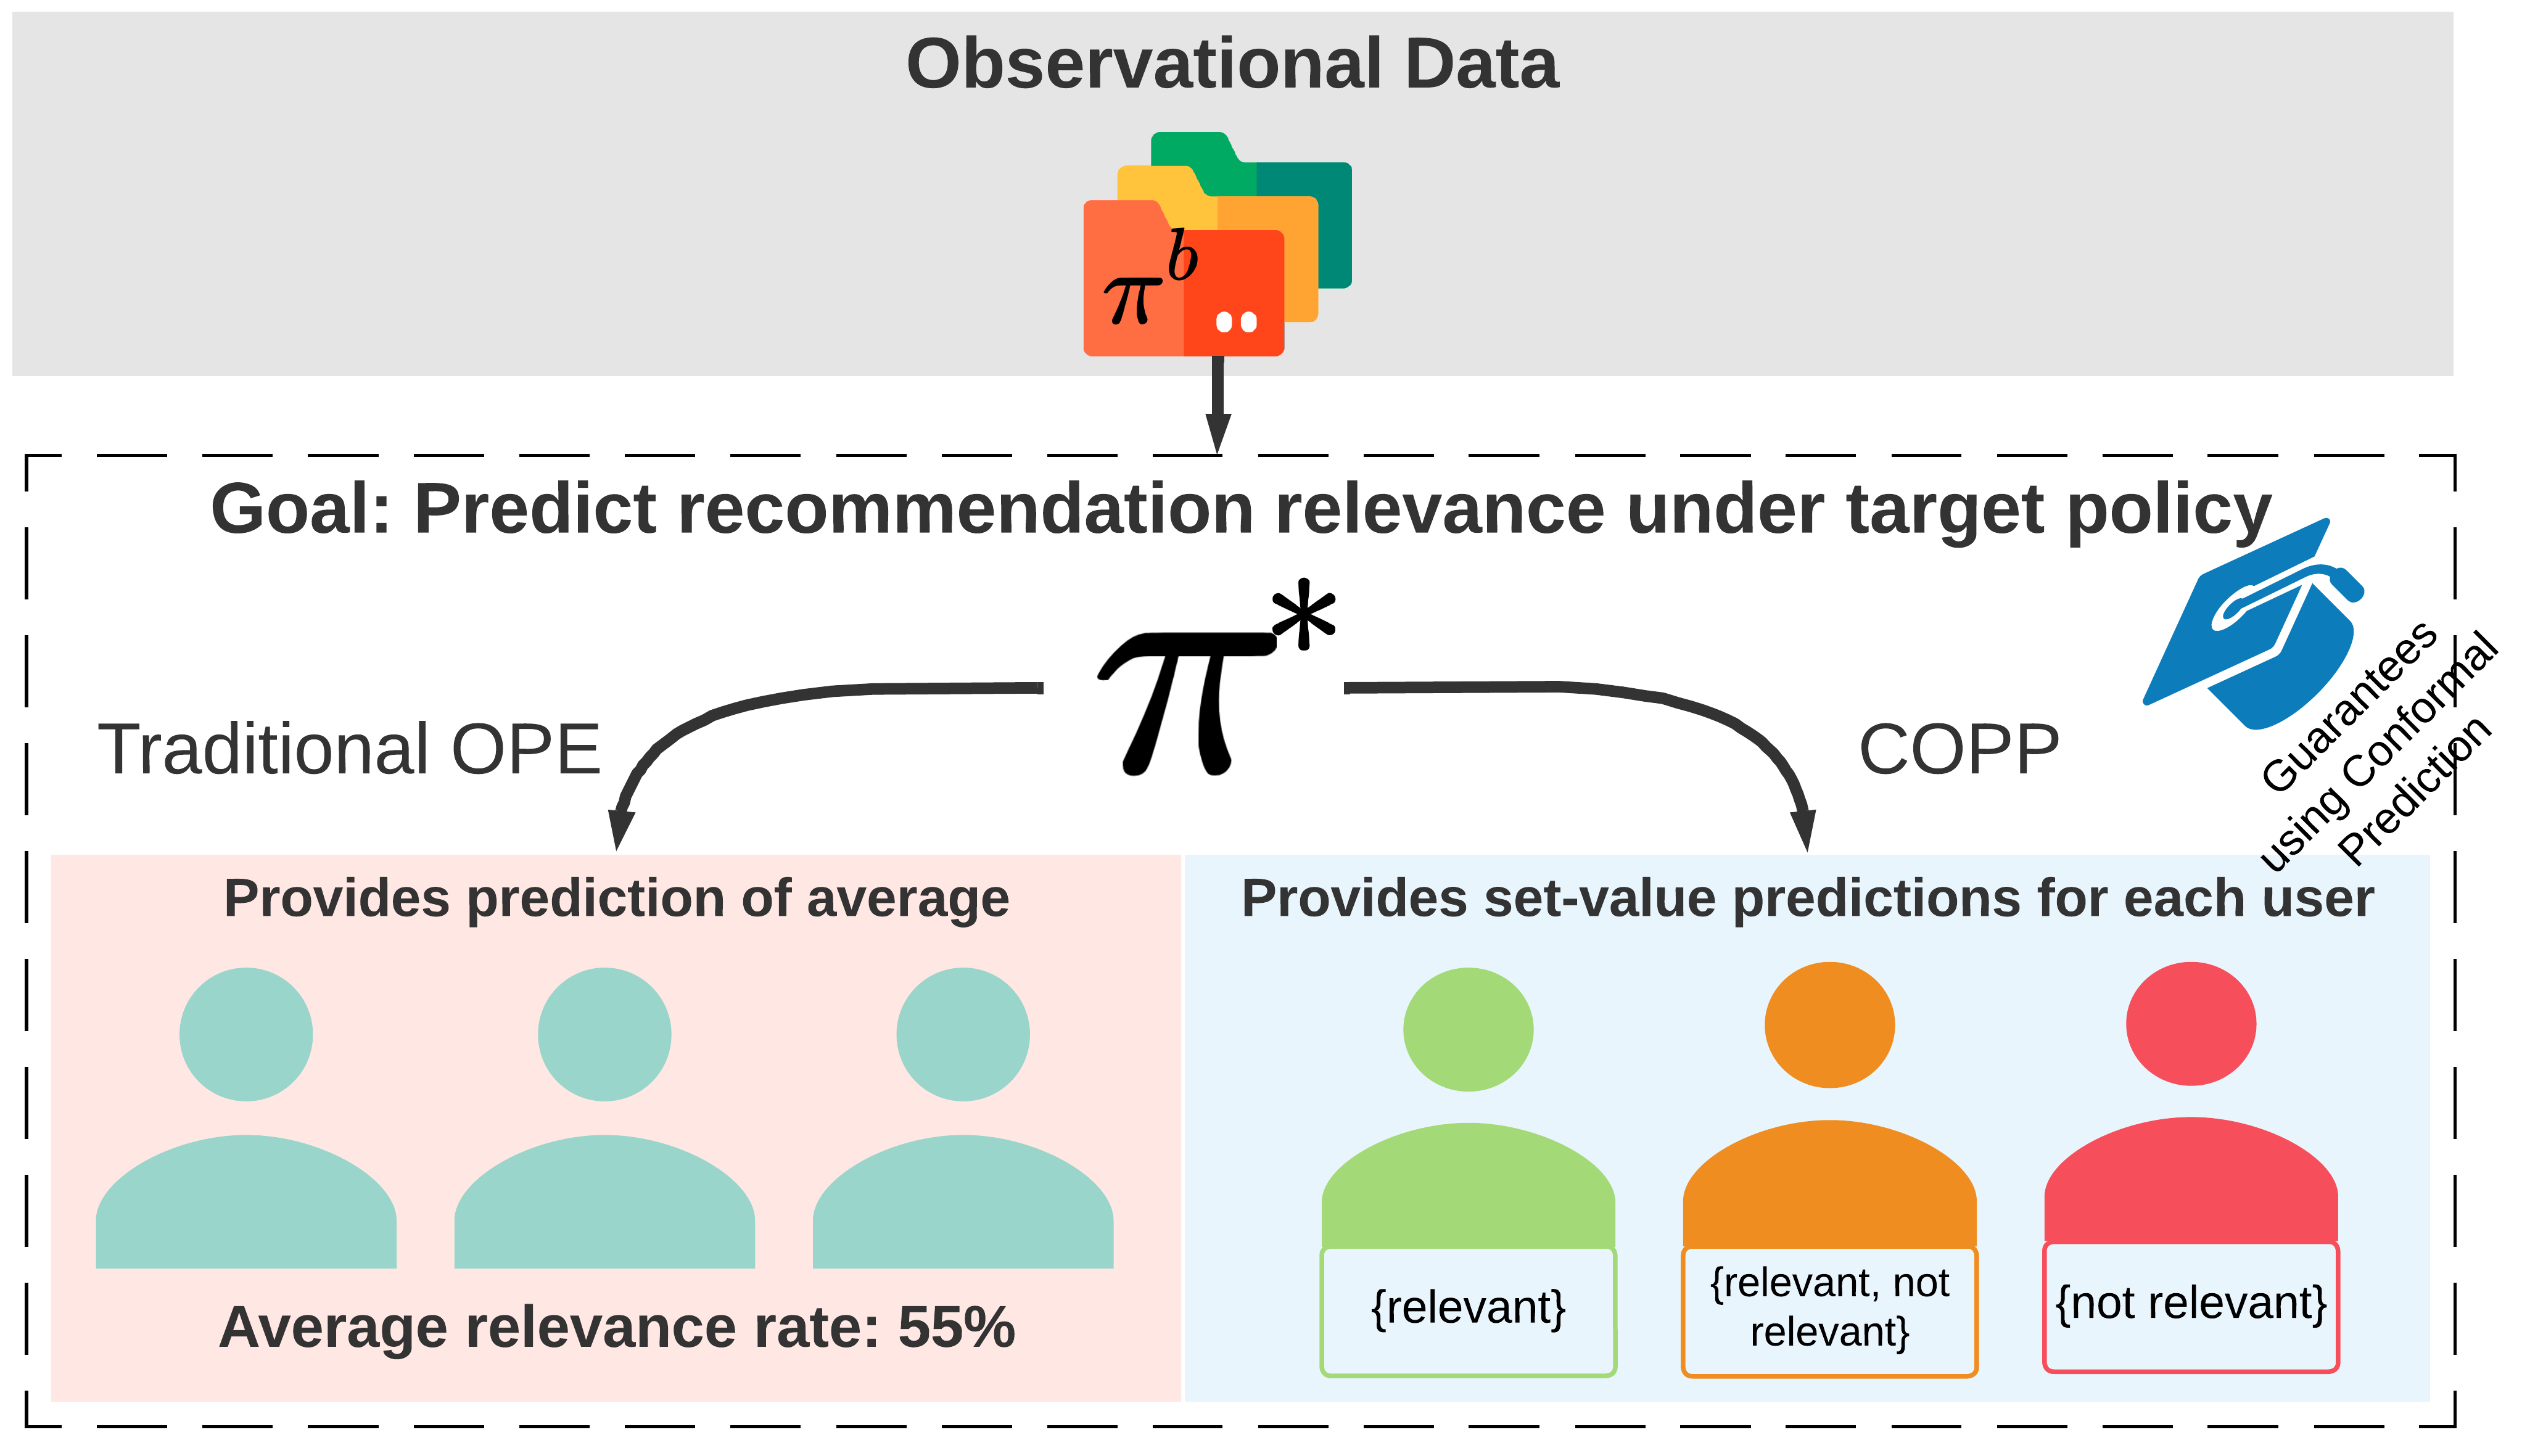
\includegraphics[height=1.85in]{figures/copp/COPP7.png}
        %  \subcaption{Conformal Off-Policy Prediction compared to standard off-policy evaluation methods.}
        %  \label{fig:copp}
     \end{subfigure}%\hspace{0.8cm}%
     \begin{subfigure}[t]{0.5\textwidth}
         \centering
         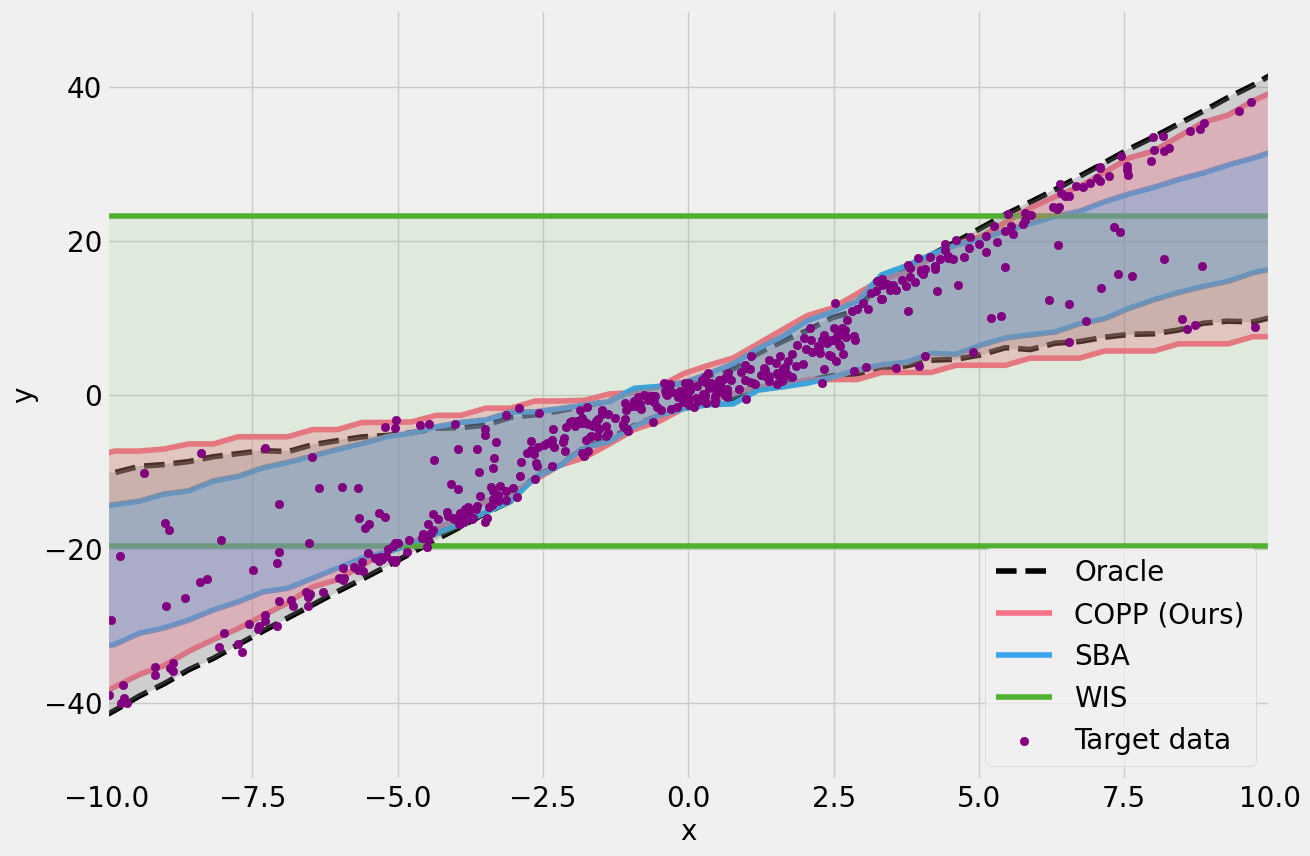
\includegraphics[height=1.85in]{figures/copp/cis-updated.png}
        %  \subcaption{$90\%$ predictive intervals for $Y$ as a function of $X$ for COPP, competing methods and the oracle.}
        %  \label{fig:cis-updated}
     \end{subfigure}

    \caption{\textbf{Left (a):} Conformal Off-Policy Prediction against standard off-policy evaluation methods. \textbf{Right (b):} $90\%$ predictive intervals for $Y$ against $X$ for COPP, competing methods and the oracle.}\label{fig:copp}
    % \label{fig:three graphs}
\end{figure}


% \begin{figure}
%     \centering
%     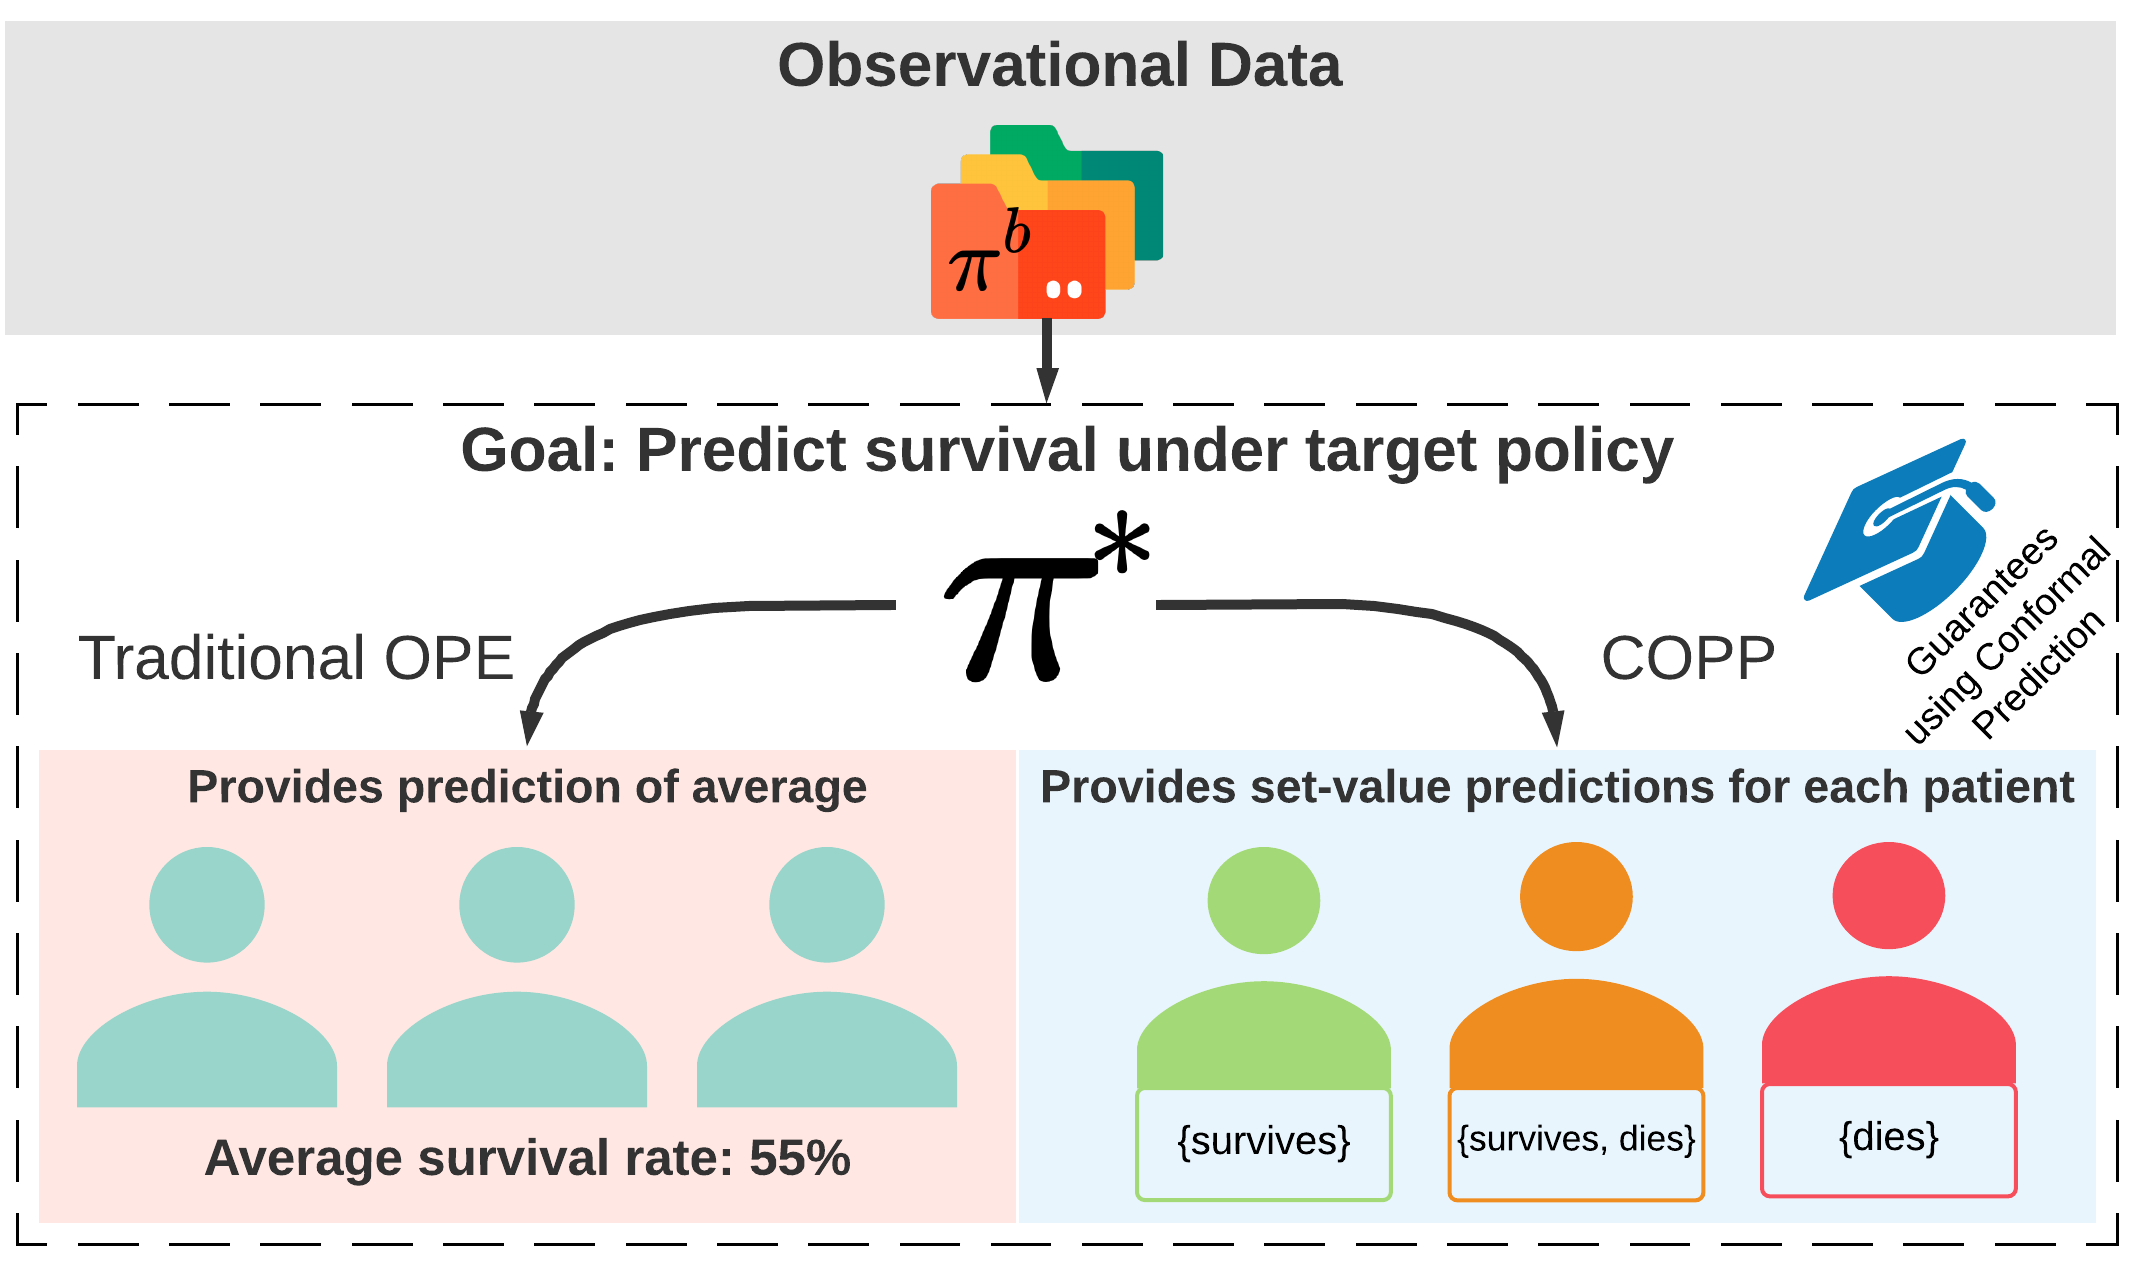
\includegraphics[width=0.5\columnwidth]{figures/copp/COPP5.png}
%     \caption{Illustration of Conformal Off-Policy Prediction compared to standard off-policy evaluation methods.}
%     \label{fig:copp}
% \end{figure}
Notable exceptions in the OPE literature are \cite{risk-assessment, chandak2021universal}. Instead of estimating bounds on the expected outcomes, \cite{risk-assessment, chandak2021universal} establish finite-sample bounds for a general class of metrics (e.g., Mean, CVaR, CDF) on the outcome. Their methods can be used to estimate quantiles of the outcomes under the target policy and are therefore robust to outliers. However, the resulting bounds do not depend on the covariates $X$ (not adaptive w.r.t. $X$). This can lead to overly conservative intervals, as we will show in our experiments and can become uninformative when the data are heteroscedastic (see Fig. \ref{fig:copp}b).

%  Instead of investigating the bounds on the expected outcomes, \cite{risk-assessment, chandak2021universal} propose an off-policy assessment in contextual bandits setting to construct bounds that enjoy finite-sample guarantees. In particular, the authors aim to construct estimators for the CDF of the return and hence are able determine quantities such as the median or the $95\%$ quantiles of the rewards, which as mentioned above, are crucial for robustness and uncertainty quantification. Note that the CDF estimators proposed by \cite{risk-assessment, chandak2021universal} do not depend on the specific $X$, and as a result the bounds obtained are not adaptive w.r.t. $X$. 

% Furthermore, while the distributional perspective without CDFs has been explored in the context of Reinforcement Learning \cite{distributional-rl}, to the best of our knowledge they do not provide any finite-sample guarantees.

% In this paper, we propose Conformal Off-Policy Prediction (COPP), a novel algorithm based on Conformal Prediction (CP) that produces predictive interval/sets for off-policy outcomes in contextual bandits (see Fig.\ref{fig:copp}a).
% To the best of our knowledge, this is the first method to obtain predictive intervals in the off-policy setting that enjoys both finite-sample theoretical guarantees and adaptivity w.r.t.\ the covariates $X$.
% % We achieve this by using conformal prediction (CP), a distribution-free uncertainty quantification method pioneered by \cite{vovk2005algorithmic}.
% %and can be used on top of any black-box model.
% Unlike previous work, which assumed a deterministic target and discrete action space, our approach is valid for stochastic target policies and continuous action spaces, which lifts the restriction of previous related work to deterministic targets and discrete actions.
% %, our approach can be applied to both deterministic and stochastic target policies, as well as discrete and continuous actions spaces.}

% In this paper, we propose Conformal Off-Policy Prediction (COPP), a novel algorithm for constructing predictive interval/sets for off-policy outcomes in contextual bandits (see Fig.\ref{fig:copp}a).
In this paper, we propose Conformal Off-Policy Prediction (COPP), a novel algorithm that uses Conformal Prediction (CP) \citep{vovk2005algorithmic} to construct predictive interval/sets for outcomes in contextual bandits (see Fig.\ref{fig:copp}a) using an observational dataset.
COPP enjoys both finite-sample theoretical guarantees and adaptivity w.r.t.\ the covariates $X$, and, to the best of our knowledge, is the first such method based on CP that can be applied to stochastic policies and continuous action spaces.
% To the best of our knowledge, COPP is the first such method that enjoys both finite-sample theoretical guarantees and adaptivity w.r.t.\ the covariates $X$.
% Unlike earlier work, our approach can be applied to stochastic policies and continuous action spaces.
% Unlike related work involving CP, our approach can be applied to both deterministic and stochastic target policies
% We achieve this via conformal prediction (CP), a distribution-free uncertainty quantification method pioneered by \cite{vovk2005algorithmic}.
%and can be used on top of any black-box model.

% % {\color{red} Our approach also applies to stochastic target policies which have not been considered by previous work on CP.}
% % Most importantly, CP produces predictive intervals that have finite-sample coverage guarantees, i.e. the interval will contain the ground truth outcome with a certain user pre-specified threshold $\alpha$.
% Our paper also makes the following additional contributions.
% (i)
% % Our approach is widely applicable: previous work involving CP has been limited to deterministic policies and discrete action spaces, while our method applies also for discrete and continuous.
% % Our approach is more widely applicable than previous work involving CP, and can be used for stochastic policies and continuous action spaces.
% % Our approach lifts restrictions present in related work involving CP, 
% % \R{Unlike related work involving CP, our approach can be applied to both deterministic and stochastic target policies, as well as discrete and continuous actions spaces.}
% \R{Our approach remains valid for stochastic target policies and continuous action spaces, which lifts the restriction of previous related work to deterministic targets and discrete actions.} %, our approach can be applied to both deterministic and stochastic target policies, as well as discrete and continuous actions spaces.}
% % \R{Unlike related work involving CP, our approach can be applied to both deterministic and stochastic target policies}
% % (ii) We provide theoretical guarantees for COPP, including finite-sample guarantees on marginal coverage and asymptotic guarantees on conditional coverage.
% (ii) We provide a theoretical analysis of COPP, including finite-sample guarantees on marginal coverage and asymptotic guarantees on conditional coverage.
% (iii) We show empirically that COPP outperforms standard methods in terms of coverage and predictive interval width when assessing new policies. 

% {\color{red} Our approach also applies to stochastic target policies which have not been considered by previous work on CP.}
% Most importantly, CP produces predictive intervals that have finite-sample coverage guarantees, i.e. the interval will contain the ground truth outcome with a certain user pre-specified threshold $\alpha$.
In summary, our contributions are: 
% (i) We adapt results from the CP literature to construct predictive intervals for the outcome $Y$ under a new policy which are adaptive w.r.t.\ $X$.
% (i) We construct valid predictive intervals for bandit outcomes that applies in more general settings (stochastic policies and continuous actions) than previous work.
(i) We propose an application of CP to construct predictive intervals for bandit outcomes that is more general (applies to stochastic policies and continuous actions) than previous work.
% Our approach is widely applicable: previous work involving CP has been limited to deterministic policies and discrete action spaces, while our method applies also for discrete and continuous.
% Our approach is more widely applicable than previous work involving CP, and can be used for stochastic policies and continuous action spaces.
% Our approach lifts restrictions present in related work involving CP, 
% \R{Unlike related work involving CP, our approach can be applied to both deterministic and stochastic target policies, as well as discrete and continuous actions spaces.}
% \R{Our approach avoids various restrictions of earlier work, being valid for stochastic target policies and continuous action spaces.} %, our approach can be applied to both deterministic and stochastic target policies, as well as discrete and continuous actions spaces.}
% \R{Unlike related work involving CP, our approach can be applied to both deterministic and stochastic target policies}
(ii) We provide theoretical guarantees for COPP, including finite-sample guarantees on marginal coverage and asymptotic guarantees on conditional coverage.
(iii) We show empirically that COPP outperforms standard methods in terms of coverage and predictive interval width when assessing new policies. 

\subsection{Problem Setup}\label{sec:problem_setup}

\begin{comment}
% \begin{wrapfigure}{r}{0.22\textwidth}
\begin{figure}
    \centering
    \includegraphics[width=0.15\textwidth]{diagram1.pdf}
    \caption{Causal graph of our problem setup. The action $A$ is shaded to illustrate that we are ``integrating out'' the effect of the actions through the policy when predicting $Y$ from $X$.}
    \label{fig:OPE_conformal}
\end{figure}
% \end{wrapfigure}
\end{comment}
Let $\mathcal{X}$ be the covariate space (e.g., user  data), $\mathcal{A}$ the action space (e.g., recommended items) and $\mathcal{Y}$ the outcome space (e.g., relevance to the user).
We allow both $\mathcal{A}$ and $\mathcal{Y}$ to be either discrete or continuous.
In our setting, we are given logged observational data $\mathcal{D}_{obs}=\{x_i, a_i, y_i \}_{i=1}^{n_{obs}}$ where actions are sampled from a behavioural policy $\pi^{b}$, i.e. $A \mid x \sim \pi^{b}(\cdot\mid x)$ and $Y \mid x,a \sim P(\cdot \mid x, a)$. We assume that we do not suffer from unmeasured confounding. At test time, we are given a state $x^{test}$ and a new policy $\pi^*$. While $\pi^{b}$ may be unknown, we assume the target policy $\pi^*$ to be known.
% \begin{comment}
% \begin{align*}
%     \text{Standard OPE} \qquad & \mathbb{E}_{(X, Y) \sim P^{\pi^*}_{X,Y}}[Y] \\
%     \text{Huang} \qquad & \mathbb{E}_{(X, Y) \sim P^{{\pi^*}}_{X,Y}} [\varphi(Y)], \varphi \in \Phi \\
%     \text{Us} \qquad &  \hat{C} \text{ s.t. } 1- \alpha \hspace{-0.05cm}\leq  \tarprob(Y \in \hat{C}(X)) \hspace{-0.05cm}\leq 1- \alpha + o_{n_{obs}}(1)
% \end{align*}
% \end{comment}
% \begin{comment}
% % Properties of interest: 1. adaptivity w.r.t x 2. capturing of the variability in outcomes 3. finite sample guarantees. 
% In this paper we aim to construct intervals $\hat{C}(x)$ on the outcome $Y$ which are (i) dependent on $x$, (ii) capture the variability in outcomes $Y$ and (iii) provide finite sample guarantees. Current explored methodologies lack at least one of these properties (see Table [] in section). 
% In particular, property (ii) can be achieved if $\hat{C}(x)$ captures the true outcome $Y$ with any pre-specified probability $1-\alpha$. One way to express this formally is as follows:
% \begin{align}
%      \hspace{-0.24cm}1- \alpha \hspace{-0.05cm}\leq  \tarprob(Y \in \hat{C}(X)) \hspace{-0.05cm}\leq 1- \alpha + o_{n_{obs}}(1) \label{guarantee}
% \end{align}
% where $n_{obs}$ is the size of available observational data and $P^{\pi^*}_{X,Y}$ is the joint distribution of $(X,Y)$ under target policy $\pi^*$. The probability is taken over the joint distribution of $(X, Y)$, meaning that the interval holds in the marginal sense in $X$ (marginal coverage) and not for a given $X=x$ (conditional coverage). In Section \ref{sec:cond_cov}, we provide additional regularity conditions under which not only marginal but also conditional coverage holds. Moreover, given that we are interested in the outcomes under $\pi^*$, the intervals $\hat{C}(x)$ are not conditioned on a specific $a$, but rather on $\pi^*$. 
% In this paper, we construct $\hat{C}(x)$ which satisfies \eqref{guarantee} along with the properties (i)-(iii), using the CP framework, which we will introduce in the following section. 
% % Our proposed methodology uses CP to construct $\hat{C}(x)$ and provides finite-sample coverage guarantees on the outcomes $Y$ given a current state $X$ and a target policy $\pi^* (a\mid x)$, hence allowing us to be confident in terms of the outcomes, when deploying a new policy.
% % \textbf{Explanation of the objective: } 
% % The :
% % Standard OPE & \mathbb{E}_{(X, Y) \sim P^{\pi^*}_{X,Y}}[Y] & (1) x (2) x (3) \tick
% % Huang et al & \mathbb{E}_{(X, Y) \sim P^{\pi^*}_{X,Y}}[\phi(Y]) & (1) \tick 2(x) (3) \tick
% % In this setting the quantities of interests in the current literature are:
% % \begin{align*}
% %     \text{Standard OPE} \qquad & \mathbb{E}_{(X, Y) \sim P^{\pi^*}_{X,Y}}[Y] \\
% %     \text{Huang} \qquad & \mathbb{E}_{(X, Y) \sim P^{{\pi^*}}_{X,Y}} [\varphi(Y)], \varphi \in \Phi
% % \end{align*}
% % However, none of these objectives take into account take into account both the finite sample guarantees and the adaptivity w.r.t. $x$. Hence we propose to construct predictive intervals on the outcomes which are adaptive w.r.t. $x$, and provide finite sample guarantees
% In standard OPE literature the main objective is to estimate $\mathbbm{E}[sth]$
% \end{comment}
% \textbf{Our goal} is to obtain predictive intervals/sets, $\hat{C}(x^{test})$, for a given $\alpha \in (0,1)$, which satisfy:
% \begin{align}
% \text{$P_{Y(a)}(y \mid X = x)$ for each $a$} \\
% \text{$C_a$ such that $\mathbb{P}(Y(a) \in C_a(X) \mid X = x) \geq 1 - \alpha$, for each $a$} \\
% \text{$C_a$ such that $\mathbb{P}(Y(a) \in C(X)) \geq 1 - \alpha$ for each $a$}
% \end{align}
% \begin{align}
%      \hspace{-0.24cm}1- \alpha \hspace{-0.05cm}\leq  \tarprob(Y \in \hat{C}(X)) \hspace{-0.05cm}\leq 1- \alpha + o_{n_{obs}}(1) \label{guarantee}
% \end{align}
% where $n_{obs}$ is the size of available observational data and $P^{\pi^*}_{X,Y}$ is the joint distribution of $(X,Y)$ under target policy $\pi^*$. Note that the probability is taken over the joint distribution of $(X, Y)$, meaning that the interval holds in the marginal sense in $X$ (marginal coverage) and not for a given $X=x$ (conditional coverage).  In Section \ref{sec:cond_cov}, we provide additional regularity conditions under which not only marginal but also conditional coverage holds.
% % The challenges in this case are to account for the shift in policy and obtain guarantees on the predictive interval $\hat{C}(X)$.
% To this end, we will use the CP framework to construct predictive intervals in order to assess a new policy. Our proposed methodology provides theoretical coverage guarantees on the outcome $Y$ given a current state $X$ and a target policy $\pi^* (a\mid x)$, hence allowing us to be confident in terms of the outcomes, when deploying a new policy.
% Huang et al.\ obtain a method for obtaining a richer evaluation of a given policy.
% Specifically, they estimate the $\varphi(p^{\pi^\ast}_{X,Y})$ for a more general class of functions $\varphi$ than just the expectation operator.
% While this allows for a much richer understanding of $\pi^\ast$, its expressiveness is still in some respects limited, as is clear from the fact that it does not depend on $X$, but only on $P_{X,Y}^{\pi^\ast}$.
% 
% The guarantees they get are usually only asymptotic, meaning that they approximate this quantity with 

% Existing methods focus on evaluating $\mathbb{E}_{(X, Y)\sim P^{\pi^*}_{X,Y}}[Y]$.
% This is useful for comparing two policies directly because it is just a single number, but does not provide a rich understanding of the behaviour of the policy on a per item basis.

% In this work, we present a method that avoids some of these shortcomings.
% Specifically, we construct a set-valued function $\hat{C}(x)$ that takes as input a covariate and outputs a \emph{subset} of $\mathcal{Y}$ rather than just a single point.
% This subset is guaranteed to contain the true value of $Y$ with a certain probability.
% Specifically, we obtain the guarantee:
% \[
% \tarprob(Y \in \hat{C}(X)) \geq 1 - \alpha.
% \]
% Moreover, we will show this guarantee holds for our method regardless of any distributional assumptions on $X$ and $Y$, and regardless of the size of the data we have available to us.

We consider the task of rigorously quantifying the performance of $\pi^*$ without any distributional assumptions on $X$ or $Y$. Many existing approaches estimate $\mathbb{E}_{\pi^*}[Y]$, which is useful for comparing two policies directly as they return a single number. However, the expectation does not convey fine-grained information about how the policy performs for a specific value of $X$, nor does it account for the uncertainty in the outcome $Y$.

Here, we aim to construct intervals/sets on the outcome $Y$ which are (i) adaptive w.r.t. $X$, (ii) capture the variability in the outcome $Y$ and (iii) provide finite-sample guarantees. Current methods lack at least one of these properties (see Sec. \ref{sec:related_work}). One way to achieve these properties is to construct a set-valued function of $x$, $\hat{C}(x)$ which outputs a \emph{subset} of $\mathcal{Y}$. Given any finite dataset $\mathcal{D}_{obs}$, this subset is guaranteed to contain the true value of $Y$ with any pre-specified probability, i.e.
\begin{align}
     \hspace{-0.24cm}1- \alpha \hspace{-0.05cm}\leq  \tarprob(Y \in \hat{C}(X)) \hspace{-0.05cm}\leq 1- \alpha + o_{n_{obs}}(1) \label{guarantee}
\end{align}
where $n_{obs}$ is the size of available observational data and $P^{\pi^*}_{X,Y}$ is the joint distribution of $(X,Y)$ under target policy $\pi^*$. In practice, $\hat{C}(x)$ can be used as a diagnostic tool downstream for a granular assessment of likely outcomes under a target policy. The probability in (\ref{guarantee}) is taken over the joint distribution of $(X, Y)$, meaning that \eqref{guarantee} holds marginally in $X$ (marginal coverage) and not for a given $X=x$ (conditional coverage). In Sec. \ref{sec:cond_cov}, we provide additional regularity conditions under which not only marginal but also conditional coverage holds. Next, we introduce the Conformal Prediction framework, which allows us to construct intervals $\hat{C}(x)$ that satisfy \eqref{guarantee} along with properties (i)-(iii). 

\section{Background}
Conformal prediction \citep{vovk2005algorithmic, shafer2008tutorial} is a methodology that was originally used to compute distribution-free prediction sets for regression and classification tasks. Before introducing COPP, which applies CP to contextual bandits, we first illustrate how CP can be used in standard regression.

% In this section, we illustrate the application of CP in a standard regression setting. 

% For illustrative purposes, we will consider the former in this section.
% we have considered a standard regression problem in this section.

\subsection{Standard Conformal Prediction} 
% Conformal prediction \cite{shafer2008tutorial, vovk2005algorithmic} is a methodology used to compute distribution-free prediction intervals. It was classically designed for regression and classification problems.       

% We split the available observations $\mathcal{D}_{obs}=\{X_i,Y_i \}_{i=1}^{n_{obs}}$ into a \emph{calibration} set $\mathcal{D}_{cal} = \{X_i, Y_i\}_{i\in \mathcal{I}_{cal}}$, where $\mathcal{I}_{cal}=\{1,\dots,n\}$, and a \emph{training} set $\mathcal{D}_{tr} = \{X_i^0, Y_i^0\}_{i\in \mathcal{I}_{tr}}$ where $\mathcal{I}_{tr}=\{1,\dots,N\}$.

% $\mathcal{D}_{tr} =  \mathcal{D}_{obs} \setminus \mathcal{D}_{cal}$ (of size $N$) onto which a regression model $\hat{f}$ is trained. The data in the calibration set are assumed to be i.i.d. from an arbitrary distribution $P_{X,Y}$. 

Consider the problem of regressing $\mbox{Y} \in \mathcal{Y}$ against $X\in \mathcal{X}$.
Let $\hat{f}$ be a model trained on the \emph{training} data $\mathcal{D}_{tr} = \{X_i^0, Y_i^0\}_{i=1}^m \overset{\textup{i.i.d.}}{\sim} P_{X,Y}$ and let the \emph{calibration} data $\mathcal{D}_{cal} = \{X_i, Y_i\}_{i=1}^n \overset{\textup{i.i.d.}}{\sim} P_{X,Y}$ be independent of $\mathcal{D}_{tr}$. Given a desired coverage rate $1-\alpha \in (0,1)$, we construct a band $\hat{C}_n:\mathcal{X}\rightarrow \{\text{subsets of }\mathcal{Y}\}$, based on the calibration data such that, for a new i.i.d. test data $(X,Y) \sim P_{X,Y}$,
\begin{align}
    1-\alpha \leq \mathbb{P}_{(X,Y)\sim P_{X,Y}}(Y\in \hat{C}_n(X)) \leq 1-\alpha + \frac{1}{n+1}, \label{cp_guarantee}
\end{align}
where the probability is taken over $X,Y$ and $\mathcal{D}_{cal} = \{X_i, Y_i\}_{i=1}^n$ and is conditional upon $\mathcal{D}_{tr}$.

% \yw{so there's $X_i$ in  train set and $X_i$ in calibration set? Note both index sets start at 1, so not disjoint. but we have i in $I_cal$ and $I_tr$ one is from 1 to N and the other from N+1 to N+n. Read your paragraph above. I think you've updated your definition of $I_{cal}$ to be disjoint. Note that there is inconsistency with indexing of $X_{n+1}$, $Y_{n+1}$ now. oh i see you are right let me fix the notation now should be 1 to n and then n+1 to n+N}

In order to obtain $\hat{C}_n$ satisfying \eqref{cp_guarantee}, we introduce a non-conformity score function $V_i = s(X_i, Y_i)$, e.g., $(\hat{f}(X_i) - Y_i)^2$. We assume here $\{V_i\}_{i=1}^n$ have no ties almost surely. Intuitively, the non-conformity score $V_i$ uses the outputs of the predictive model $\hat{f}$ on the calibration data, to measure how far off these predictions are from the ground truth response. Higher scores correspond to worse fit between $x$ and $y$ according to $\hat{f}$. We define the empirical distribution of the scores $\{V_i\}_{i=1}^n \cup \{\infty\}$
\begin{align}\label{eq:std_emp_score}
 \hat{F}_{n} \coloneqq \frac{1}{n+1} \sum_{i=1}^n \delta_{V_i} + \frac{1}{n+1}\delta_{\infty}  
\end{align}
with which we can subsequently construct the conformal interval $\hat{C}_n$ that satisfies \eqref{cp_guarantee} as follows:
\begin{align}
    \hat{C}_n(x) \coloneqq \{y: s(x,y) \leq \eta\} \label{eq:interval}
\end{align}
where $\eta$ is an empirical quantile of $\{V_i\}_{i=1}^n$, i.e. $\eta = \text{Quantile}_{1-\alpha}(\hat{F}_{n})$ is the $1-\alpha$ quantile.

Intuitively, for roughly $100\cdot(1-\alpha) \%$ of the calibration data, the score values will be below $\eta$. Therefore, if the new datapoint $(X, Y)$ and $\mathcal{D}_{cal}$ are i.i.d., the probability $\p(s(X,Y) \leq \eta)$ (which is equal to $\p(Y \in \hat{C}_n(X))$ by \eqref{eq:interval}) will be roughly $1-\alpha$. Exchangeability of the data is crucial for the above to hold. In the next section we will explain how \cite{tibshirani2020conformal} relax the exchangeability assumption.
% Hence, due to the i.i.d. assumption of the calibration and test data, it would not make sense to include $y$'s that induce a score higher than $\eta$ when targeting $100\cdot(1-\alpha) \%$ coverage guarantees. It should also be noted that exchangeability\footnote[1]{Exchangeability is sufficient and we do not need i.i.d.} of the data is crucial for the above to hold. In the next section we will explain how \cite{tibshirani2020conformal} relax this assumption.

% In essence, $\hat{C}_n(x)$ will only contain $y$'s for which the score is ``not too big'' i.e. is less than the $\lceil(n+1)(1-\alpha)\rceil/n$ quantile of the scores in the calibration data. Note that due to exchangeability and as long as the $s(x,y)$ is below the quantile, we can guarantee that the resulting interval will contain the ground truth with probability at least $1-\alpha$. 
% The original formulation of CP relies only on exchangeability of the calibration and test data. A brief summary of CP steps is given in algorithm \ref{cp}. Note that here we use the notation Quantile$(\beta; F)$ to denote the level $\beta$ quantile of a distribution F, i.e. for $Z\sim F$,
% \[
%     \text{Quantile}(\beta; F) = \inf \{z : \mathbb{P}(Z\leq z) \geq \beta \}
% \]

% It can be shown that the predictive intervals $\hat{C}_n(x)$ obtained through algorithm \ref{cp} satisfy the following guarantee
% \[
% 1-\alpha \leq \mathbb{P}(Y_{n+1}\in \hat{C}_n(X_{n+1})) \leq 1-\alpha + \frac{1}{n+1}
% \]
% \begin{algorithm}
% \SetAlgoLined
% \textbf{Inputs:} Trained model $\hat{f}$; calibration data $\{X_i, Y_i\}_{i=1}^n$; New data point $x$, confidence level $\alpha$\\
% \textbf{Output:} Confidence set $\hat{C}_n(x)$ which satisfies (\ref{cp_guarantee})\\
% Define the score function $s(X,Y)\in\mathbb{R}$ (larger scores encode worse fit between $X$ and $Y$).\;
% \For{i = 1, \dots, n}{
% $V_i \coloneqq s(X_i, Y_i)$\;
% }
% Define the empirical distribution $\hat{F}_{n} \coloneqq \frac{1}{n+1} \sum_{i=1}^n \delta_{V_i} + \frac{1}{n+1}\delta_{\infty}$\;
% For a new data point $x$, $\hat{C}_n(x) \coloneqq \{y: s(x,y) \leq \text{Quantile}(\lceil(n+1)(1-\alpha)\rceil/n, \hat{F}_{n})\}$\;
% \textbf{Return} $\hat{C}_n(x)$
%   \caption{Conformal prediction algorithm}
%   \label{cp}
% \end{algorithm}

\subsection{Conformal Prediction under covariate shift}\label{CP_cov_shift}
\cite{tibshirani2020conformal} extend the CP framework beyond the setting of exchangeable data, by constructing valid intervals even when the calibration data and test data are not drawn from the same distribution. The authors focus on the \textit{covariate shift} scenario i.e. the distribution of the covariates changes at test time:
\begin{align}
    &(X_i, Y_i) \overset{\textup{i.i.d}}{\sim} P_{X,Y} = P_X \times P_{Y\mid X}, \quad i = 1, \dots, n \nonumber \\
    &(X, Y) \sim \tilde{P}_{X,Y} = \tilde{P}_{X} \times P_{Y\mid X},~\text{independently}\nonumber
\end{align}

% \begin{center}
% \begin{tabular}{l}
%             \small $(X_i, Y_i) \overset{\textup{i.i.d}}{\sim} P_{X,Y} = P_X \times P_{Y\mid X}, \quad i = 1, \dots, n$\\ 
%             \small $(X, Y) \sim \tilde{P}_{X,Y} = \tilde{P}_{X} \times P_{Y\mid X},~\text{independently}$
% \end{tabular}
% \end{center}
where the ratio $w(x)\coloneqq\mathrm{d}\tilde{P}_{X}/\mathrm{d}P_{X}(x)$ is known.
The key realization in \cite{tibshirani2020conformal} is that the requirement of \textit{exchangeability} in CP can be relaxed to a more general property, namely \textit{weighted exchangeability} (see Def. \ref{def:weighted_exch}). 
% The key realization is by firstly noting that the calibration and test data are \textit{weighted exchangeable}, which is more general property than \textit{exchangeability}.
% Secondly, if we know the ratio of test to calibration covariate likelihoods, we can define $w(x) = d\tilde{P}_{X}(x)/dP_{X}(x)$. 
They propose a weighted version of conformal prediction, which shifts the empirical distribution of non-conformity scores, $\hat{F}_{n}$, at a point $x$, using weights $w(x)$. This adjusts $\hat{F}_{n}$ for the covariate shift, before picking the quantile $\eta$: $$\hat{F}_{n}^{x} \coloneqq  \sum_{i=1}^n p_i^w(x) \delta_{V_i} + p_{n+1}^w(x)\delta_{\infty}\quad \textup{ where,}$$ 
\begin{align*}
    p_i^{w}(x) = \frac{w(X_i)}{\sum_{j=1}^n w(X_j) + w(x)}, \quad p_{n+1}^{w}(x) = \frac{w(x)}{\sum_{j=1}^n w(X_j) + w(x)}.
\end{align*}

% \begin{align}
%     \hat{F}_{n}^{x} \coloneqq  \sum_{i=1}^n p_i^w(x) \delta_{V_i} + p_{n+1}^w(x)\delta_{\infty}, \nonumber
% \end{align}



% $p_i^w(x) \propto w(X_i)$ for $i \in \{1,...,N\}$, $p^w_{n+1}(x)\propto w(x)$ with $\sum_{i=1}^{n+1} p^w_i(x)=1$. \yw{much notational problem here. what's $x$? I can't parse "$p^w_i(x) \propto w(X_i)$". Is it $n$ or $N$?}  

In standard CP (without covariate shift), the weight function satisfies $w(x)=1$ for all $x$, and we recover \eqref{eq:std_emp_score}. Next, we construct the conformal prediction intervals $\hat{C}_n$ as in standard CP using \eqref{eq:interval} where $\eta$ now depends on $x$ due to $p^w_i(x)$. The resulting intervals, $\hat{C}_n$, satisfy: 
% \yw{not sure I understand this point re dependence on $x$. what's $x$ actually?}
% \begin{align*}
%     1-\alpha \leq \mathbb{P}_{(X,Y)\sim \tilde{P}_{X, Y}}(Y\in \hat{C}_n(X)) \leq 1-\alpha + cn^{1/r-1}    
% \end{align*}
\begin{align*}
     \mathbb{P}_{(X,Y)\sim \tilde{P}_{X, Y}}(Y\in \hat{C}_n(X)) \geq 1-\alpha    
\end{align*}
As mentioned previously in Sec. \ref{sec:problem_setup}, the above demonstrates marginal coverage guarantees over test point $X$ \faaiz{and calibration dataset $\mathcal{D}_{cal}$, not conditional on a given $X=x$ or a fixed $\mathcal{D}_{cal}$}.  We will discuss this nuance later on in Sec. \ref{sec:cond_cov}. In addition, previous work by \citeauthor{vovk2012} shows that conditioned on a single calibration dataset, standard CP can achieve coverage that is `close' to the required coverage with high probability. However, this has not been extended to the case where the distribution shifts. This is out of the scope of this paper and an interesting future direction. 


\begin{algorithm}[!htp]
\SetAlgoLined
\textbf{Inputs:} Observational data $\mathcal{D}_{obs}=\{X_i, A_i, Y_i\}_{i=1}^{n_{obs}}$, conf. level $\alpha$, a score function $s(x,y)\in\mathbb{R}$, new data point $x^{test}$, target policy $\pi^*$ \;
\textbf{Output:} Predictive interval $\hat{C}_n(x^{test})$\;
Split $\mathcal{D}_{obs}$ into training data ($\mathcal{D}_{tr}$) and calibration data ($\mathcal{D}_{cal}$) of sizes $m$ and $n$ respectively\;
Use $\mathcal{D}_{tr}$ to estimate weights $\hat{w}(\cdot, \cdot)$ using \eqref{weight-est}\;
Compute $V_i \coloneqq s(X_i, Y_i)$ for $(X_i, A_i, Y_i) \in \mathcal{D}_{cal}$\;
Let $\hat{F}_{n}^{x, y}$ be the weighted distribution of scores 
$\hat{F}_{n}^{x, y} \coloneqq  \sum_{i=1}^n p_i^{\hat{w}}(x, y) \delta_{V_i} + p_{n+1}^{\hat{w}}(x, y)\delta_{\infty}$\\
where $p_i^{\hat{w}}(x, y) = \frac{\hat{w}(X_i, Y_i)}{\sum_{j=1}^n \hat{w}(X_j, Y_j) + \hat{w}(x, y)}$ and $p_{n+1}^{\hat{w}}(x, y) = \frac{\hat{w}(x, y)}{\sum_{j=1}^n \hat{w}(X_j, Y_j) + \hat{w}(x, y)}$\;
% \textcolor{red}{Define the empirical distribution $\hat{F}_{n} \coloneqq  \sum_{i=1}^n p_i^w(x) \delta_{V_i} + p_{n+1}^w(x)\delta_{\infty}$}\;
% \textcolor{red}{where $p_i^w(x) = \frac{w(X_i)}{\sum_{j=1}^n w(X_j) + w(x)}$ and $p_{n+1}^w(x) = \frac{w(x)}{\sum_{j=1}^n w(X_j) + w(x)}$}\;


% Define the empirical distribution of the scores as:
% $$
% \hat{\mathcal{F}}_{n}^{x, y} \coloneqq 
% \begin{cases}
% \hat{F}_{n} &\text{for standard CP }   \eqref{eq:std_emp_score}\\ 
% \hat{F}_{n}^{x}  &\text{for cov. shifted CP }  \eqref{eq:cov_shift_emp_score}\\
% \hat{F}_{n}^{x, y}  &\text{for policy shifted CP }  \eqref{score-dist-pshift}\\
% \end{cases}
% $$
For $x^{test}$ construct:
% $$\hat{C}_n(x^{test}) \coloneqq \{y: s(x^{test},y) \leq \text{Quantile}(1-\alpha, \hat{F}_{n})\}$$
% $$\hat{C}_n(x^{test}) \coloneqq \{y: s(x^{test},y) \leq \text{Quantile}(1-\alpha, \hat{F}_{n}^{x})\}$$
$
    \hat{C}_n(x^{test})\hspace{-0.1cm} \coloneqq \{y: s(x^{test},y) \leq \text{Quantile}_{1-\alpha}(\hat{F}_{n}^{x^{test}, y})\} \nonumber
$

\textbf{Return} $\hat{C}_n(x^{test})$
  \caption{Conformal Off-Policy Prediction (COPP)}
  \label{cp_covariate_shift}
\end{algorithm}

Thus \cite{tibshirani2020conformal} show that the CP algorithm can be extended to the setting of covariate shift with the resulting predictive intervals satisfying the coverage guarantees when the weights are known. The extension of these results to approximate weights was proposed in  \cite{lei2020conformal} and is generalized to our setting in Sec. \ref{sec:theory}. 
\section{Conformal Off-Policy Prediction (COPP)}
% \subsection{Conformal Prediction with policy shift}
In the contextual bandits introduced in Sec. \ref{sec:problem_setup}, we assume that the observational data $\mathcal{D}_{obs} = \{x_i, a_i, y_i\}_{i=1}^{n_{obs}}$ is generated from a behavioural policy $\pi^b$. At inference time we are given a new target policy $\pi^*$ and want to provide intervals on the outcomes $Y$ for covariates $X$ that satisfy \eqref{guarantee}.

% Before diving deeper into our proposed method, we would like to highlight certain aspects of the problem. Firstly, the key difference between covariate shifted CP and our problem setting is the following: For covariate shifted CP, we are provided with an unseen data point $x^{test}$ for which we want to find a predictive interval $\hat{C}(x^{test})$. However, in our setting we are given $x^{test}$ \textbf{and} a target policy $\pi^*$, i.e. a function and hence needs to be taken care of appropriately. Secondly, contrary to {tibshirani2020conformal}, who look into a shift in $P_X$, we are instead interested in the shift in policies, which, as we show in this section, corresponds to a conditional shift in $P_{Y|X}$.
The key insight of our approach is to consider the following joint distribution of $(X,Y)$:
% \begin{align*}
%     P^{\pi^{b}}(x, y) \hspace{-0.1cm} &= \hspace{-0.1cm} P(x) \int P(y| x, a) \textcolor{red}{\pi^{b}(a|x)} \mathrm{d}a  =P(x) \textcolor{red}{P^{\pi^{b}}(y|x)} \\
%     P^{\pi^*}(x, y)\hspace{-0.1cm} &= \hspace{-0.1cm} P(x)\int P(y| x, a) \textcolor{red}{\pi^*(a|x)}  \mathrm{d}a = P(x)\textcolor{red}{P^{\pi^*}(y|x)}
% \end{align*}
% \begin{center}
% \begin{tabular}{c}
%             \small $P^{\pi^{b}}(x, y) \hspace{-0.1cm} = \hspace{-0.1cm} P(x) \int P(y| x, a) \textcolor{red}{\pi^{b}(a|x)} \mathrm{d}a  =P(x) \textcolor{red}{P^{\pi^{b}}(y|x)}$\\ 
%             \small $P^{\pi^*}(x, y)\hspace{-0.1cm} = \hspace{-0.1cm} P(x)\int P(y| x, a) \textcolor{red}{\pi^*(a|x)}  \mathrm{d}a = P(x)\textcolor{red}{P^{\pi^*}(y|x)}$
% \end{tabular}
% \end{center}
\begin{align*}
    P^{\pi^{b}}(x, y)=& P(x) \int P(y| x, a) \textcolor{red}{\pi^{b}(a|x)} \mathrm{d}a  =P(x) \textcolor{red}{P^{\pi^{b}}(y|x)} \\
    P^{\pi^*}(x, y) =& P(x)\int P(y| x, a) \textcolor{red}{\pi^*(a|x)}  \mathrm{d}a = P(x)\textcolor{red}{P^{\pi^*}(y|x)}
\end{align*}

Therefore, the change of policies from $\pi^b$ to $\pi^*$ causes a shift in the joint distributions of $(X, Y)$ from $P^{\pi^{b}}_{X, Y}$ to $P^{\pi^*}_{X, Y}$. More precisely, a shift in the conditional distribution of $Y|X$. As a result, our problem boils down to using CP in the setting where the conditional distribution $P^{\pi^{b}}_{Y\mid X}$ changes to $P^{\pi^{*}}_{Y \mid X}$ due to the different policies, while the covariate distribution $P_X$ remains the same. 
% =\mathrm{d}P^{\pi^{*}}_{X,Y}/\mathrm{d}P^{\pi^{b}}_{X,Y}(x,y)

Hence our problem is not concerned about covariate shift as addressed in \cite{tibshirani2020conformal}, but instead uses the idea of \textit{weighted exchangeability} to extend CP to the setting of policy shift. To account for this distributional mismatch, our method shifts the empirical distribution of non-conformity scores at a point $(x, y)$ using the weights $w(x,y) = \mathrm{d}P^{\pi^{*}}_{X,Y}/\mathrm{d}P^{\pi^{b}}_{X,Y}(x,y) = \mathrm{d}P^{\pi^{*}}_{Y|X}/\mathrm{d}P^{\pi^{b}}_{Y|X}(x,y)$:
\begin{align}
   \textstyle  \hat{F}_{n}^{x, y} &\coloneqq \sum_{i=1}^n p_i^w(x, y)\delta_{V_i} + p_{n+1}^w(x,y)\delta_\infty, \label{score-dist-pshift}
\end{align}
\begin{align*}
p_i^{w}(x, y)= \frac{w(X_i, Y_i)}{\sum_{j=1}^n w(X_j, Y_j) + w(x, y)}, \quad
p_{n+1}^{w}(x, y) = \frac{w(x, y)}{\sum_{j=1}^n w(X_j, Y_j) + w(x, y)}. 
\end{align*}


% \begin{center}
% \end{center}
% Our work builds upon the idea of conformal prediction under covariate shift proposed by \cite{tibshirani2020conformal}  exploited to quantify uncertainty in individual treatment effects by \cite{lei2020conformal}. 
% In our problem, the main challenge arises from the fact that there is a distributional mismatch between calibration ($\mathcal{D}_{cal}\subset \mathcal{D}_{obs}$) and test data. The observational data is generated using a behaviour policy $\pi^b$, whereas the predictive intervals that we seek must hold under data generated from a different target policy $\pi^*$ (for which we have no data). This shift in distribution means that standard CP can no longer be used. However, as we show next,
% This observation thus allows us to assess unseen policies $\pi^*$ based on observational data collected using $\pi^b$. 
% We note that, similar to \cite{tibshirani2020conformal}, we can use the idea of \textit{weighted exchangeability} to extend CP to our setting. 
% the calibration and test data in our setting are weighted exchangeable, with weights $w(x,y) =\mathrm{d}P^{\pi^{*}}_{X,Y}/\mathrm{d}P^{\pi^{b}}_{X,Y}(x,y)= \mathrm{d}P^{\pi^{*}}_{Y|X}/\mathrm{d}P^{\pi^{b}}_{Y|X}(x,y)$. Hence, we can extend the weighted version of CP to account for policy shift in the empirical distribution of non-conformity scores:
% $p_i^w(x, y) \propto w(X_i, Y_i)$ for $i \in \{1,...,n\}$, $p^w_{n+1}(x, y)\propto w(x, y)$ with $\sum_{i=1}^{n+1} p^w_i(x, y)=1$.
% where $p_{i}^w(x, y) \coloneqq \frac{w(X_i, Y_i)}{\sum_{i=1}^n w(X_i, Y_i) + w(x,y)}$, $p_{n+1}^w(x, y) \hspace{-0.1cm} \coloneqq \hspace{-0.1cm} \frac{w(x,y)}{\sum_{i=1}^n w(X_i, Y_i) + w(x,y)}$. 
The intervals are then constructed as below which we call Conformal Off-Policy Prediction (Alg. \ref{cp_covariate_shift}).
% As before, the predictive intervals can be constructed using
\begin{align}
    \hat{C}_n(x^{test}) \coloneqq \{y: s(x^{test},y) \leq \eta(x^{test}, y)\} \hspace{0.2cm} \textup{where, }  \eta(x, y) \coloneqq \text{Quantile}_{1-\alpha}( \hat{F}_{n}^{x, y}). \label{cp-sets}
\end{align}
% We call this Conformal Off-Policy Prediction (Alg. \ref{cp_covariate_shift}).

\paragraph{Remark}
    The weights $w(x, y)$ in \eqref{score-dist-pshift} depend on $x$ and $y$, as opposed to only $x$. In particular, finding the set of $y$'s satisfying \eqref{cp-sets} becomes more complicated than for the standard covariate shifted CP which only requires a single computation of $\eta(x)$ for a given $x$ as shown in \eqref{eq:interval}. In our case however, we have to create a $k$ sized grid of potential values of $y$ for every $x$ to find $\hat{C}_n(x)$. This operation is embarrassingly parallel and hence does not add much computational overhead compared to the standard CP, especially because CP mainly focuses on scalar predictions.


\subsection{Estimation of weights $w(x, y)$}\label{sec:weights}
So far we have been assuming that we know the weights $w(x, y)$ exactly. However, in most real-world settings, this will not be the case. Therefore, we must resort to estimating $w(x, y)$ using observational data. In order to do so, we first split the observational data into training ($\mathcal{D}_{tr}$) and calibration ($\mathcal{D}_{cal}$) data. Next, using $\mathcal{D}_{tr}$, we estimate $\hat{\pi}^b(a\mid x) \approx \pi^b(a \mid x)$ and $\hat{P}(y \mid x, a) \approx P(y \mid x, a)$ (which is independent of the policy). We then compute a Monte Carlo estimate of weights using the following:
% \begin{align}\label{CP_new_weights}
%     w(x, y) = \frac{\int P(y|x, a) \textcolor{red}{\pi^*(a|x)} da}{\int P(y| x, a) \textcolor{red}{\pi^b(a|x)} da}
% \end{align} 
% which can subsequently be estimated using the monte carlo estimator:
\begin{align}
    \hat{w}(x, y) &= \frac{\tfrac{1}{h}\sum_{k=1}^{h} \hat{P}(y|x, A^*_k)}{\tfrac{1}{h} \sum_{k=1}^{h} \hat{P}(y|x, A_k)} \approx \frac{\int P(y|x, a) \textcolor{red}{\pi^*(a|x)} \mathrm{d}a}{\int P(y| x, a) \textcolor{red}{\pi^b(a|x)} \mathrm{d}a},  \label{weight-est}
\end{align}
where $A_k\sim \hat{\pi}^b(\cdot \mid x),~ A_k^* \sim  \pi^*(\cdot \mid x)$ and $h$ is the number of Monte Carlo samples.

\begin{importantresultwithtitle}[title=Why not construct intervals using \text{$\hat{P}(y|x, a)$} directly?]\noindent
    % \paragraph{Why not construct intervals using $\hat{P}(y|x, a)$ directly?} 
    We could directly construct predictive intervals $\hat{C}_n(x)$ over outcomes by sampling $$Y_j \overset{\textup{i.i.d.}}{\sim} \hat{P}^{\pi^*}(y|x) = \int \hat{P}(y|x, a)\pi^*(a|x)\mathrm{d}a.$$ However, the coverage of these intervals directly depends on the estimation error of $\hat{P}(y|x, a)$. This is not the case in COPP, as the coverage does not depend on $\hat{P}(y|x, a)$ directly but rather on the estimation of $\hat{w}(x, y)$ (see Prop. \ref{prop2}). We hypothesize that this indirect dependence of COPP on $\hat{P}(y|x, a)$ makes it less sensitive to the estimation error. In Sec. \ref{sec:exp}, our empirical results support this hypothesis as COPP provides more accurate coverage than directly using $\hat{P}(y|x, a)$ to construct intervals. Lastly, in Appendix \ref{sec:alternate_weights_est} we show how we can avoid estimating $\hat{P}(y|x, a)$ by proposing an alternative method for estimating the weights directly. We leave this for future work.
\end{importantresultwithtitle}
% This is not the case in COPP, as the coverage does not depend on $\hat{P}(y|x, a)$ directly but rather on the estimation of $\hat{w}(x, y)$ (see Prop. \ref{prop2}). 
% Given $\hat{P}(y|x, a)$, one could directly construct predictive intervals over outcomes $\hat{C}(x)$ by sampling $y_j \overset{i.i.d}{\sim} \hat{P}^{\pi^*}(y|x) = \int \hat{P}(y|x, a)\pi^*(a|x)\mathrm{d}a$. However, the coverage of these intervals will directly depend on the estimation error of $\hat{P}(y|x, a)$. This is not the case in COPP, as the coverage does not depend on $\hat{P}(y|x, a)$ directly but rather on the estimation of $\hat{w}(x, y)$ (see prop. \ref{prop2}). In the Appendix \red{ref}, we show that consistency of the weights $\hat{w}(x, y)$ does not imply the consistency of $\hat{P}(y|x, a)$. In Section \ref{sec:exp}, we also show that empirically, COPP provides more accurate coverage than directly using $\hat{P}(y|x, a)$ to construct the predictive intervals. 



% The coverage guarantee in COPP relies on consistent estimation of weights $\hat{w}(x, y)$, which we show in (\red{add reference}) does not imply the consistency of $\hat{P}(y|x, a)$. 

% Note, given that the behavioural policy and $P(y|x, a)$ are unknown, we use estimates $\hat{\pi}^b$ and $\hat{P}(y|x, a)$. Next, $\hat{w}(x, y)$ can be well estimated as a monte carlo estimator.

% Having established this relationship between different policies and the conditional distribution, we will proof in the following section that we can retain the theoretical finite-sample coverage guarantees using our modified conformal prediction framework. 

\section{Theoretical Guarantees}\label{sec:theory}
\subsection{Marginal Coverage}

In this section we provide theoretical guarantees on marginal coverage $\tarprob(Y \in \hat{C}_n(X))$ for the cases where the weights $w(x, y)$ are known exactly as well as when they are estimated. Using the idea of \textit{weighted exchangeability}, we extend \cite[Theorem 2]{tibshirani2020conformal} to our setting. 
% \begin{definition}[Weighted exchangeability]\label{exchangeability}
% Random variables $V_1, \dots, V_n$ are said to be \textit{weighted exchangeable} with weight functions $w_1, \dots, w_n$, if the density $f$ of their joint distribution can be factorized as
% \begin{align}
%     f(v_1, \dots, v_n) = \prod_{i=1}^n w_i(v_i) g(v_1, \dots, v_n)
% \end{align}
% where $g$ is any function that does not depend on the ordering of its inputs, i.e. $g(v_{\sigma(1)}, \dots, v_{\sigma(n)}) = g(v_1, \dots, v_n)$ for any permutation $\sigma$ of $1, \dots, n$.
% \end{definition}
% We observe that the calibration data $\{X_i, Y_i\}_{i=1}^n \overset{\textup{i.i.d.}}{\sim} P^{\pi^b}(X,Y)$ and test data point $(X_{n+1},Y_{n+1}) \sim P^{\pi^*}(X,Y)$ are indeed weighted exchangeable given the weights in the lemma below.
% \begin{lemma}\label{exchangeability_lemma}
% Let $Z_i = (X_i, Y_i) \in \mathbb{R}^d \times \mathbb{R}$, $i=1,...,n+1$, be such that $\{(X_i, Y_i)\}_{i=1}^n \overset{\textup{i.i.d.}}{\sim}P^{\pi^b}(X,Y)$ and $(X_{n+1}, Y_{n+1}) \sim P^{\pi^*}(X,Y)$. Then $Z_1, \dots, Z_{n+1}$ are weighted exchangeable with weights $w_i \equiv 1$, $i\leq n$ and $w_{n+1}(X,Y) = P^{\pi^*}(X,Y)/P^{\pi^b}(X,Y)$.
% \end{lemma}
% Using the weighted exchangeability property between the calibration and test data from Lemma \ref{exchangeability_lemma}, we extend Theorem 2 in \cite{tibshirani2020conformal} to our setting.

\begin{proposition}\label{coverage_theorem}
Let $\{X_i, Y_i\}_{i =1}^n \overset{\textup{i.i.d.}}{\sim}P^{\pi^b}_{X,Y}$ be the calibration data. For any score function $s$, and any $\alpha \in (0,1)$, define the conformal predictive interval at a point $x\in \mathbb{R}^d$ as 
$$\hat{C}_n(x) \coloneqq \left\{y \in \mathbb{R}: s(x, y) \leq \eta(x,y) \right\}$$
where $\eta(x, y) \coloneqq \text{Quantile}_{1-\alpha}( \hat{F}_{n}^{x, y})$, and $\hat{F}_{n}^{x, y}$ is as defined in \eqref{score-dist-pshift} with exact weights $w(x,y)$.
If $P^{\pi^*}(y| x)$ is absolutely continuous w.r.t. $P^{\pi^b}(y| x)$,
% If the non-conformity scores $\{V_i\}_{i=1}^n$ have no ties almost surely, and $P^{\pi^*}(y\mid x)$ is absolutely continuous w.r.t.\ $P^{\pi^b}(y\mid x)$,
then $\hat{C}_{n}$ satisfies
$$\tarprob(Y \in \hat{C}_{n}(X)) \geq 1-\alpha \nonumber.$$
% If we additionally have that for some $r > 1$
% \[
% (\expb[w(X,Y)^r])^{1/r} \leq M_r < \infty,
% \]
% then we also obtain an upper bound
% \begin{align}
%     % 1-\alpha \leq
%     \tarprob(Y\in \hat{C}_n(X)) \leq 1-\alpha + cn^{1/r-1}, \nonumber
% \end{align}
% where $c$ is a positive constant depending only on $M_r$ and $r$.
\end{proposition}
\begin{comment}
\begin{proposition}\label{coverage_theorem}
Let $\{X_i, Y_i\}_{i=1}^n \overset{\textup{i.i.d.}}{\sim}P^{\pi^b}_{X,Y}$ and $(X_{n+1}, Y_{n+1}) \sim P^{\pi^*}_{X, Y}$ be independent of $\{X_i, Y_i\}_{i=1}^n$. For any score function $s$, and any $\alpha \in (0,1)$, define the conformal predictive interval at a point $x\in \mathbb{R}^d$ the equation below:
\begin{align}
    &\hat{C}_n(x) = \left\{y \in \mathbb{R}: s(x, y) \leq \eta(x,y) \right\} \nonumber
\end{align}
where $\eta(x, y) \coloneqq \text{Quantile}_{1-\alpha}( \hat{F}_{n}^{x, y})$, and $\hat{F}_{n}^{x, y}$ is as defined in \eqref{score-dist-pshift}.
% where $V_i \hspace{-0.1cm} \coloneqq \hspace{-0.1cm} s(X_i, Y_i)$ and

% \begin{align}
%     &\eta(x,y) \hspace{-0.1cm} \coloneqq \hspace{-0.1cm}\textup{Quantile}_{1-\alpha}\hspace{-0.13cm}\left(\sum_{i=1}^n p_i^w(x, y)\delta_{V_i} + p_{n+1}^w(x,y)\delta_\infty \right) \nonumber \\
%     &w(x,y) \hspace{-0.1cm} \coloneqq \hspace{-0.1cm} \frac{P^{\pi^*}(y \mid x)}{P^{\pi^b}(y \mid x)} \nonumber\\
%     &p_{i}^w(x, y) \hspace{-0.1cm} \coloneqq \hspace{-0.1cm} \frac{w(X_i, Y_i)}{\sum_{i=1}^n w(X_i, Y_i) + w(x,y)} \nonumber \\
%     &p_{n+1}^w(x, y) \hspace{-0.1cm} \coloneqq \hspace{-0.1cm} \frac{w(x,y)}{\sum_{i=1}^n w(X_i, Y_i) + w(x,y)}. \nonumber
% \end{align}

% Then $\hat{C}_{n}$ satisfies
% \begin{align}
%     \mathbb{P}(Y_{n+1} \in \hat{C}_{n}(X_{n+1})) \geq 1-\alpha \label{eq:our_guarantee}
% \end{align}
\end{proposition}
\end{comment}
% \textcolor{blue}{by the continuous mapping theorem, this is also consistent estimator such that $\hat{w}(x, y) \rightarrow w(x, y)$ when $m_c, n \rightarrow \infty$.}
% paragraph{Notes on Theorem \ref{coverage_theorem}:} It is important to note that the weights $w(x, y)$ in Theorem \ref{coverage_theorem} depend on $x$ and $y$, as opposed to only depend on $x$ in \cite{tibshirani2020conformal}(see section \ref{CP_cov_shift}). This is the main difference between the our methods and adds to the practical challenge when constructing CP sets. In particular, finding the set of $y$'s that satisfy \eqref{eq:cover_policy_interval} becomes more challenging, given that the standard covariate shifted CP by \cite{tibshirani2020conformal}, only requires a single computation of $\eta(x)$ for a given $x$ as shown in  \eqref{eq:interval}. 
% In our case however, $\eta(x, y)$ depends on both $x$ and $y$ and therefore, in order to find $\hat{C}_n(x)$, we create a $k$ sized grid of potential values of $y$ for every $x$. This operation is embarrassingly parallel and hence does not add much computational overhead compared to the conventional method, especially because CP mainly focuses on 1-D predictions. This additional challenge of having to create a grid is specific to the regression tasks and simplifies to a simple enumeration of the labels in the classification setting.
% \begin{comment}
% 1. make it clear that grid is on the values of y.
% 2. mention that y is scalar, so the grid points lie on real points.
% 3. This is specific to when y is continuous, in the case of discrete y, we can simply enumerate over all values.
% \end{comment}
% Hence, the main method that we propose in this paper circumvents the need to take the union over all the most likely actions, but instead will use the weights in \eqref{CP_new_weights} to create the interval. By using \eqref{CP_new_weights}, we can integrate out the policy \textbf{before} computing our conformal intervals and thus allowing us to avoid the aforementioned problem of taking the union. Therefore, we will firstly, estimate the weights as follows:
% \begin{align}
%     \hat{w}(x, y) = \frac{\sum_{k=1}^{m_c} p^*(y|x, a_k)}{\sum_{k=1}^{m_c} p(y|x, a_k)}
% \end{align}
% and by Slutsky's theorem, this is a consistent estimator and $\hat{w}(x, y) \rightarrow w(x, y)$ when $m_c \rightarrow \infty$.
% Next, in order to be able to compute the conformal interval that satisfies 
% \begin{algorithm}
% \SetAlgoLined
% \textbf{Inputs:} Estimated weights $\hat{w}(x, y)$ \eqref{weight-est}; calibration data $\{x_i, a_i, y_i\}_{i=1}^n$ (where $a|x \sim \hat{\pi}^b$); score function $s(x, y)$; New data point $x^{test}$ and confidence level $\alpha$\\
% \textbf{Output:} Confidence set $\hat{C}_n(x)$ which satisfies (\ref{eq:our_guarantee})\\
% % Define the score function $s(x,y)\in\mathbb{R}$ (larger scores encode worse fit between $x$ and $Y=y$)\;
% \For{i = 1, \dots, n}{
% $V_i \coloneqq s(x_i, y_i)$
% }
% \textcolor{red}{Define the empirical distribution $\hat{F}_{n}^{x, y} \coloneqq  \sum_{i=1}^n p_i^{\hat{w}}(x, y) \delta_{V_i} + p_{n+1}^{\hat{w}}(x, y)\delta_{\infty}$}
% \textcolor{red}{where $p_i^{\hat{w}}(x, y) = \frac{\hat{w}(x_i, y_i)}{\sum_{j=1}^n \hat{w}(x_j, y_j) + \hat{w}(x, y)}$ and $p_{n+1}^{\hat{w}}(x, y) = \frac{\hat{w}(x, y)}{\sum_{j=1}^n \hat{w}(x_j, y_j) + \hat{w}(x, y)}$}\\
% % \textcolor{red}{and $\hat{w}(x, y) \approx \frac{P^{\pi^*} (y \mid x)}{P_{\hat{\pi}^b} (y \mid x)}$}\\
% For a new data point $x$, $\hat{C}_n(x) \coloneqq \{y: s(x,y) \leq \text{Quantile}_{1-\alpha}(\hat{F}_{n}^{x, y})\}$
% \textbf{Return} $\hat{C}_n(x)$
%   \caption{Conformal prediction for OPE under conditional shift}
%   \label{cp_conditional_shift}
% \end{algorithm}
% what we are we adapting? 
% our setting is fundamentally different from shift setting,
% we show that the results of \cite{tibshirani2020conformal} can be extended to our setting of conditional shift, 
% However, it's important to note that in our setting, the weights are equal to ratio of conditionals instead of ratio of covariates, and hence depend on y. This adds complexity when constructing the conformal predictive intervals. A more detailed discussion of this can be found in section [reference].
% the weights depend on y as well. 
% Proposition 1:
% Theorem 1 assumes that we know the weights, this will very likely not be true in most real world settings. Hence, we will need to approximate the weights w(X, Y) using the available training data. In the case of CP under covariate shift, \cite{lei2020conformal} showed that even when the weights are approximated i.e. $\hat{w}(\cdot) = w(\cdot)$, we can still provide both upper and lower bounds on the coverage, albeit slightly modified with an error term $\delta_{\omega}$see Eq.([]). We show that this result be straightforwardly extended to our setting.
% As we have already pointed out, our setting is fundamentally different from the covariate shift setting. In our setting, it is the conditional distribution $P(Y\mid X)$ that is being shifted between calibration and test data, as opposed to the covariate distribution $P(X)$. However, 
Proposition \ref{coverage_theorem} assumes  exact weights $w(x, y)$, which is usually not the case. For CP under covariate shift, \cite{lei2020conformal} showed that even when the weights are approximated, i.e., $\hat{w}(x, y) \neq w(x, y)$, we can still provide finite-sample upper and lower bounds on the coverage, albeit with an error term $\Delta_w$ (defined in \eqref{delta_w}). Next, we extend this result to our setting when the weight function $w(x, y)$ is approximated as in Section \ref{sec:weights}.

\begin{proposition}\label{prop2}
Let $\hat{C}_n$ be the conformal predictive intervals obtained as in Proposition \ref{coverage_theorem}, with weights $w(x,y)$ replaced by approximate weights $\hat{w}(x,y) = \hat{w}(x,y;\mathcal{D}_{tr})$, where the training data, $\mathcal{D}_{tr}$, is fixed. Assume that $\hat{w}(x, y)$ satisfies $(\expb[\hat{w}(X,Y)^r])^{1/r} \leq M_r < \infty$ for some $r \geq 2$.
Define $\Delta_w$ as,
\begin{align}
    \Delta_w \coloneqq \tfrac{1}{2}\expb \mid \hat{w}(X,Y) - w(X,Y)\mid  \label{delta_w}.\\
    \text{Then, } \hspace{0.2cm} \tarprob(Y\in \hat{C}_n(X)) \geq 1-\alpha - \Delta_w.\nonumber
\end{align}
If, in addition, non-conformity scores $\{V_i\}_{i=1}^n$ have no ties almost surely, then we also have
\begin{align}
    \tarprob(Y\in \hat{C}_n(X)) \leq 1-\alpha + \Delta_w + cn^{1/r-1}, \nonumber
\end{align}
for some positive constant $c$ depending only on $M_r$ and $r$.
\end{proposition}
\begin{comment}
\begin{proposition}\label{prop2}
Consider Algorithm \ref{cp_covariate_shift} and assume $(X_i, Y_i) \overset{\textup{i.i.d.}}{\sim} P^{\pi^b}_{X,Y}$. First, consider the case where $\hat{w}(\cdot, \cdot) = w(\cdot, \cdot)$. 
If the non-conformity scores $\{V_i\}_{i=1}^n$ have no ties almost surely, $P^{\pi^*}(y\mid x)$ is absolutely continuous w.r.t. $P^{\pi^b}(y\mid x)$, and $(\expb[\hat{w}(X,Y)^r])^{1/r} \leq M_r < \infty$, then
\begin{align}
    1-\alpha \leq \tarprob(Y\in \hat{C}_n(X)) \leq 1-\alpha + cn^{1/r-1}, \nonumber
\end{align}
where $c$ is a positive constant depending only on $M_r$ and $r$.

In the general case where $\hat{w}(\cdot) \neq w(\cdot)$, set 
\begin{align}
    \Delta_w \coloneqq \tfrac{1}{2}\expb \mid \hat{w}(X,Y) - w(X,Y)\mid  \label{delta_w}.
\end{align}
Then, we have
\begin{align}
    1-\alpha - \Delta_w  &\leq \tarprob(Y\in \hat{C}_n(X)) \nonumber\\ 
    &\leq 1-\alpha + \Delta_w + cn^{1/r-1}.
\end{align}
\end{proposition}
\end{comment}
Proposition \ref{prop2} provides finite-sample guarantees with approximate weights $\hat{w}(\cdot, \cdot)$. Note that if the weights are known exactly then the above proposition can be simplified by setting $\Delta_w =0$. In the case where the weight function is estimated \textit{consistently}, we recover the exact coverage asymptotically. A natural question to ask is whether the consistency of $\hat{w}(x, y)$ implies the consistency of $\hat{P}(y|x, a)$; in which case one could use $\hat{P}(y|x, a)$ directly to construct the intervals. We prove that this is not the case in general and provide detailed discussion in Appendix \ref{sec:weights_estimation_app}. 

\subsection{Conditional Coverage}\label{sec:cond_cov}
So far we only considered marginal coverage \eqref{guarantee}, where the probability is over both $X$ and $Y$. Here, we provide results on conditional coverage $\p_{Y \sim P^{\pi^*}_{Y \mid X}}(Y \in \hat{C}_n(X) \mid X)$ which is a strictly stronger notion of coverage than marginal coverage \citep{foygel2021limits}. \cite{vovk2012, lei2014distribution} prove that exact conditional coverage cannot be achieved without making additional assumptions. However, we show that, in the case where $Y$ is a continuous random variable and we can estimate the quantiles of $P^{\pi^*}_{Y \mid X}$ consistently, we get an approximate conditional coverage guarantee using the below proposition.
% \begin{corollary}\label{corollary1}
% Let $N, n$ be the number of training and calibration data respectively, $\hat{w}_N(x, y)$ be an estimate of $w(x, y) = P^{\pi^*}(Y\mid X)/P^{\pi^b}(Y\mid X)$ and $\hat{C}_{N,n}(x)$ be the conformal interval resulting from algorithm \ref{cp_conditional_shift}. Assume that $(\mathbb{E}_{\pi^b}[\hat{w}(X,Y)^r])^{1/r} \leq M_r < \infty$. If the following assumption holds:
% \begin{align}
%     \lim_{N \rightarrow \infty} \mathbb{E}_{\pi^b} |\hat{w}_{N}(X, Y) - w(X, Y)|  = 0
% \end{align}
% Then, under SUTVA and the strong ignorability assumption, 
% \[
% \lim_{N, n \rightarrow \infty} \mathbb{P}_{(X,Y)\sim P^{\pi^*}}(Y\in \hat{C}_{N, n}(X)) = 1- \alpha
% \]
% \end{corollary}
\begin{proposition}[Asymptotic Conditional Coverage]\label{conditional-res}
Let $m, n$ be the number of training and calibration data respectively, $\hat{q}_{\beta, m} (x)= \hat{q}_{\beta, m} (x; \mathcal{D}_{tr})$ be an estimate of the $\beta$-th conditional quantile $q_\beta (x)$ of $P^{\pi^*}_{Y \mid X=x}$, $\hat{w}_m(x, y) = \hat{w}_m(x, y; \mathcal{D}_{tr})$ be an estimate of $w(x,y)$ and $\hat{C}_{m,n}(x)$ be the conformal interval resulting from algorithm \ref{cp_covariate_shift} with score function $s(x, y) = \max \{y - \hat{q}_{\alpha_{hi}} (x), \hat{q}_{\alpha_{lo}} (x) - y \}$ where $\alpha_{hi} - \alpha_{lo} = 1 - \alpha$. Assume that the following hold:
\begin{enumerate}
    \item $\lim_{m \rightarrow \infty} \expb |\hat{w}_{m}(X, Y) -  w(X, Y)|  = 0$.
    % \item $\p_{Y\sim P^{\pi^*}(\cdot \mid X)}(\max \{Y - q_{\alpha_{hi}}(X), q_{\alpha_{lo}}(X) - Y \} \leq 0 \mid X) = 1-\alpha $ almost surely.
    \item there exists $r, b_1, b_2 > 0$ such that $P^{\pi^*}(y \mid x) \in [b_1, b_2]$ uniformly over all $(x, y)$ with $y \in [q_{\alpha_{lo}}(x) - r, q_{\alpha_{lo}}(x) + r] \cup [q_{\alpha_{hi}}(x) - r, q_{\alpha_{hi}}(x) + r]$,
    %\item $\p_{(X, Y) \sim P^{\pi^*}}(w(X,Y) < \infty) = 1$, and there exists $\delta, M > 0$ such that $(\mathbb{E}_{\pi}[\hat{w}_N(X, Y)^{1+\delta}])^{1/(1+\delta)} \leq M$ 
    \item  $\exists k > 0$ s.t. $\lim_{m\rightarrow\infty} \mathbb{E}_{X\sim P_X}[H^k_{m}(X)] = 0$
    where $$H_m(x) = \max\{|\hat{q}_{\alpha_{lo}, m}(x) - q_{\alpha_{lo}}(x)|, |\hat{q}_{\alpha_{hi}, m}(x) - q_{\alpha_{hi}}(x)|\}$$
\end{enumerate}
Then for any $t > 0$, we have that $ \lim_{m, n \rightarrow \infty} \p(\p_{Y \sim P^{\pi^*}_{Y\mid X} }(Y\in \hat{C}_{m, n}(X) \mid X) \leq 1 - \alpha - t) = 0.$
\end{proposition}

% \textbf{Remark.} 
One caveat of Prop. \ref{conditional-res} is that Assumption 3 is rather strong. In general, consistently estimating the quantiles under the target policy $\pi^*$ is not straightforward given that we only have access to observational data from $\pi^b$. While one can use a weighted pinball loss to estimate quantiles under $\pi^*$, consistent estimation of these quantiles would require a consistent estimate of the weights (see Appendix  \ref{sec:estimating_target_quantiles}). Hence, unlike \cite[Theorem 1]{lei2020conformal}, our Prop. \ref{conditional-res} is not a ``\textit{doubly robust}'' result.

\begin{importantresultwithtitle}[title=Towards group balanced coverage]\noindent \label{sec:group_balanced_cov}
\begin{comment}
Consider a subset of $(x,y)$ space, $\Omega \subset \mathcal{X} \times \mathcal{Y}$, such that $\mathbb{P}_{\pi^b}((X,Y) \in \Omega) > 0$. Conformal prediction provides us the ability to construct predictive sets, $\hat{C}_{n}^{\Omega}(x)$ which provide coverage guarantees conditional on $(X,Y) \in \Omega$ \citep{limits-conf}, i.e.
\begin{align}
    1-\alpha \leq& \mathbb{P}_{(X,Y)\sim P^{\pi^*}}(Y \in \hat{C}_{n}^{\Omega}(X) \mid (X,Y) \in \Omega) \nonumber\\ 
    \leq& 1 - \alpha + o_{n}(1) \nonumber
\end{align}
Restricting ourselves to a specific subgroup allows us to construct predictive sets which have correct coverage for these set of users, thereby ensuring ``fair'' model across groups \citep{romano2019conformalized}.
The way to construct such predictive intervals $\hat{C}_{n}^{\Omega}(x)$ is straightforward: in algorithm \ref{cp_covariate_shift}, we restrict the calibration dataset to $\{(x_i, y_i): (x_i, y_i)\in \Omega\}$. The rest of the algorithm remains the same. A more detailed discussion of this has been included in \textcolor{red}{supplementary material}.
\end{comment}
As pointed out by \cite{conf-bates}, we may want predictive intervals that have the same coverage across different groups, e.g., across male and female users \citep{Romano2020With}. Standard CP will not necessarily achieve this, as the coverage guarantee \eqref{guarantee} is over the entire population of users.
% Formally, this problem can be expressed as follows. Let $\Omega = \{\Omega_1, \cdots, \Omega_k \}$ be subsets of $\mathcal{X} \times \mathcal{Y}$ with $\tarprob((X,Y) \in \Omega_j) > 0$ for $j\in \{1, \dots, k\}$. We would like to construct  predictive intervals $\hat{C}_n^\Omega$ which satisfy 
% $
%     \tarprob(Y \in \hat{C}_n^\Omega(X) \mid (X, Y) \in  \Omega_j) \geq 1-\alpha, \nonumber
% $
% for all $j\in \{1, \dots, k\}$. 
However, we can use COPP on each subgroup separately to obtain group balanced coverage. A more detailed discussion on how to construct such intervals has been included in Appendix \ref{sec:grp-bal}.
\end{importantresultwithtitle}


\section{Related Work}\label{sec:related_work}
% \subsection{Works exploring conformal prediction under distribution shift}
\textbf{Conformal Prediction:} A number of works have explored the use of CP under distribution shift. The works of \cite{tibshirani2020conformal} and \cite{lei2020conformal} are particularly notable as they extend CP to the general setting of \textit{weighted exchangeability}.  In particular, \cite{lei2020conformal} use CP for counterfactual inference where the goal is to obtain predictive intervals on the outcomes of treatment and control groups. The authors formulate the counterfactual setting into that of covariate shift in the input space $\mathcal{X}$ and show that under certain assumptions, finite-sample coverage can be guaranteed.

Fundamentally, our work differs from \cite{lei2020conformal} by framing the problem as a shift in the conditional $P_{Y\mid X}$ rather than as a shift in the marginal $P_X$.
The resulting methodology we obtain from this then differs from \cite{lei2020conformal} in a variety of ways.
For example, while \cite{lei2020conformal} assume a deterministic target policy, COPP can also be applied to stochastic target policies, which have been used in a variety of applications, such as recommendation systems or RL applications \citep{swaminathan2016off, su2020doubly, farajtabar2018more}. 
Likewise, unlike \cite{lei2020conformal}, COPP is applicable to continuous action spaces, e.g., doses of medication administered.

% In addition, for deterministic target policies, 
In addition, when the target policy is deterministic, there is an important methodological difference between COPP and \cite{lei2020conformal}.
In particular, \cite{lei2020conformal} construct the intervals on outcomes by splitting calibration data w.r.t.\ actions.
In contrast, it can be shown that COPP uses the entire calibration data when constructing intervals on outcomes.
This is a consequence of integrating out the actions in the weights $w(x, y)$ \eqref{weight-est}, and empirically leads to smaller variance in coverage compared to \cite{lei2020conformal}.
See \ref{sec:comp_lc} for the experimental results comparing COPP to \cite{lei2020conformal} for deterministic policies.

% the abiliity to apply our method to , stochasticity, which have been used in a variety of applications. Diagnostic tool emphasis
% COPP provides a number of advantages over LC21. 
% recommendation system examples

% Furthermore, COPP can be used to construct intervals on the off-policy outcomes when the target policy is stochastic. \cite{lei2020conformal} on the other hand is restricted to deterministic policies.

% \R{Furthermore, while \cite{lei2020conformal} can be used to construct intervals on the off-policy outcomes when the target policy is deterministic, COPP can also be applied to stochastic target policies, which have been used in a variety of applications, such as recommendation systems or RL applications \cite{swaminathan2016off, su2020doubly, farajtabar2018more}. In the case where the target policy is deterministic, there is an important methodological difference between COPP and \cite{lei2020conformal}. \cite{lei2020conformal} construct the intervals on outcomes by splitting calibration data w.r.t. actions. In contrast, it can be shown that COPP uses the entire calibration data when constructing intervals on outcomes. This is a consequence of integrating out the actions in the weights $w(x, y)$ \eqref{weight-est}, and empirically leads to smaller variance in coverage compared to \cite{lei2020conformal}. See \ref{sec:comp_lc} for experimental results. Lastly, COPP can also be applied to continuous action spaces because of \eqref{weight-est}, whereas \cite{lei2020conformal} cannot.} 


% \R{

% }


% In addition, COPP can be applied to the problem of individual treatment effect (ITE) estimation (where the target policies are deterministic). However, contrary to \cite{lei2020conformal}, our methodology does not require splitting calibration data w.r.t. actions/treatments. This is a consequence of integrating out the actions when constructing the intervals. A detailed discussion of this is given in \ref{sec:lei_candes_app}.

% Since we integrate out actions in weights estimation \eqref{weight-est}, we are able to use the entire calibration dataset when constructing intervals conditioned on a specific action $a$. In contrast, \cite{lei2020conformal} require splitting calibration data w.r.t. actions to construct such intervals.

% when constructing intervals conditioned on a specific action $a$, \cite{lei2020conformal} require splitting calibration data w.r.t. actions. This is a specific case in our setting with target policy $\pi^*(A|X) = \mathbbm{1}\{A=a\}$, and our methodology allows us to use the entire calibration dataset. A more detailed discussion of this is given in \red{add ref}.
%
% which has also been explored in \cite{lei2020conformal}, is a specific case in our setting with target policy $\pi^*(A|X) = \mathbbm{1}\{A=a\}$.

% one of the problems explored in \cite{lei2020conformal} is the construction of intervals conditioned on a specific action $a$. This is a specific case in our setting with target policy $\pi^*(A|X) = \mathbbm{1}\{A=a\}$. 

% In this paper we reframe our policy shift not as a shift in the marginal distribution $P_X$ as in {tibshirani2020conformal, lei2020conformal}, but instead as a shift in the conditional distribution $P_{Y\mid X}$ while $P_X$ remains unchanged.
% Note that the problem of constructing intervals conditioned on a specific action $a$ has been explored in \cite{lei2020conformal}, and is a specific case in our setting with target policy $\pi^*(A|X) = \mathbbm{1}\{A=a\}$. In contrast to \cite{lei2020conformal}, where the authors split calibration data to construct these intervals, our methodology allows the use of entire calibration dataset.

\cite{osama2020learning} propose using CP to \textit{construct} robust policies in contextual bandits with discrete actions. Their methodology uses CP to choose actions and does not involve evaluating target policies. Hence, the problem being considered is orthogonal to ours. There has also been concurrent work adapting CP to individual treatment effect (ITE) sensitivity analysis model \citep{jin2021sensitivity, yin2021conformal}. Similar to our approach, these works formulate the sensitivity analysis problem as one of CP under the joint distribution shift $P_{X, Y}$. While our methodologies are related, the application of CP explored in these works, i.e. ITE estimation under unobserved confounding, is fundamentally different. 
% While both of our works diverge from the standard covariate shift in the input distribution $P(X)$, we are fundamentally solving different problems, In our paper we focus on the off-policy assessment whereas [refs] are concerned about ITE under unobserved confounding effects.
% \subsection{Uncertainty quantification in contextual bandits}

\textbf{Uncertainty in contextual bandits:} Recall from the introduction, that most works in this area have focused on quantifying uncertainty in expected outcome (policy value) \citep{doubly-robust, uncertainty5}. Despite providing finite sample-guarantees on the expectation, these methods do not account for the variability in the outcome itself and in general are not adaptive w.r.t. $X$, i.e. they do not satisfy properties (i), (ii) from Sec. \ref{sec:problem_setup}. \cite{risk-assessment, chandak2021universal} on the other hand, propose off-policy assessment algorithms for contextual bandits w.r.t. a more general class of risk objectives such as Mean, CVaR etc. Their methodologies can be applied to our problem, to construct predictive intervals for off-policy outcomes. However, unlike COPP, these intervals are not adaptive w.r.t. $X$, i.e. do not satisfy property (i) in Sec. \ref{sec:problem_setup}. Moreover, they do not provide upper bounds on coverage probability, which often leads to overly conservative intervals, as shown in our experiments. Lastly, while distributional perspective has been explored in reinforcement learning \citep{distributional-rl}, no finite sample-guarantees are available to the best of our knowledge.
% The authors provide an estimator for the target policy's CDF of outcomes with finite-sample guarantees, which can subsequently be used to construct approximate predictive intervals on the outcome under target policy. However, \cite{risk-assessment} do not provide upper bounds on the coverage probability, and the intervals obtained are not adaptive w.r.t. $x$. This leads to overly conservative intervals, as shown in our experiments.


% \begin{figure}
%     \centering
%     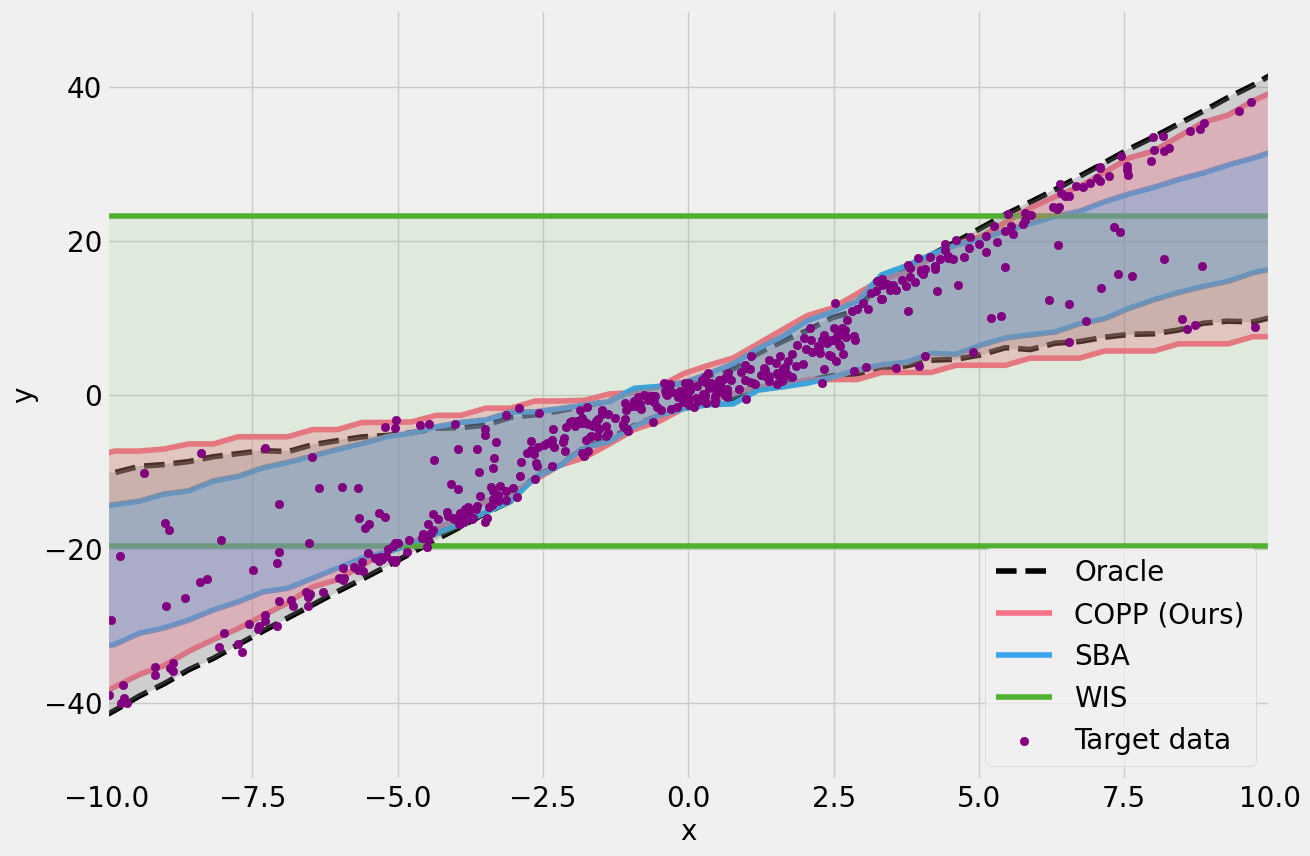
\includegraphics[width=0.50\columnwidth]{figures/copp/cis-updated.png}
%     \caption{$90\%$ predictive intervals for $Y$ as a function of $X=x$ for COPP, competing methods and the oracle.}
%     \label{fig:cis-updated}
% \end{figure}
\section{Experiments} \label{sec:exp}



\textbf{Baselines for comparison.}
Given our problem setup, there are no established baselines. Instead, we compare our proposed method COPP to the following competing methods, which were constructed to capture the uncertainty in the outcome distribution and take into account the policy shift. 
% \footnote{Link to our code has been included in a separate file}

\textbf{Weighted Importance Sampling (WIS) CDF estimator.} Given observational dataset $\mathcal{D}_{obs} = \{x_i, a_i, y_i\}_{i=1}^{n_{obs}}$, \cite{risk-assessment} proposed a non-parametric WIS-based estimator for the empirical CDF of $Y$ under $\pi^*$, 
$
\hat{F}_{WIS}(t) \coloneqq \frac{\sum_{i=1}^{n_{obs}} \hat{\rho}(a_i, x_i) \mathbbm{1}(y_i \leq t)}{\sum_{i=1}^{n_{obs}} \hat{\rho}(a_i, x_i)}
$
where $\hat{\rho}(a, x) \coloneqq \frac{\pi^*(a \mid x)}{\hat{\pi}^b(a \mid x)}$ are the importance weights. We can use $\hat{F}_{WIS}$ to get predictive intervals $[y_{\alpha/2}, y_{1-\alpha/2}]$ where $y_\beta \coloneqq \text{Quantile}_\beta(\hat{F}_{WIS})$. The intervals $[y_{\alpha/2}, y_{1-\alpha/2}]$ do not depend on $x$.



% $
% \inf_{t\in \mathbb{R}}\{t: \hat{F}_{WIS}(t) \geq \beta \}$, i.e. the quantiles of $\hat{F}_{WIS}(t)$. 

\begin{table}[t]
    \caption{Toy experiment results with required coverage $90\%$. While WIS intervals provide required coverage, the mean interval length is huge compared to COPP (see table \ref{tab:length_toy}).}
    \begin{minipage}[b]{.48\linewidth}
      \centering
      \subcaption{Mean Coverage as a function of policy shift with 2 standard errors over 10 runs.}\label{tab:coverage_toy}
      \resizebox{1\columnwidth}{!}{%
        \begin{tabular}{lccc}
\toprule
Coverage &  $\Delta_{\epsilon}=0.0$ &  $\Delta_{\epsilon}=0.1$ &  $\Delta_{\epsilon}=0.2$ \\
\midrule
COPP (Ours)            &                    \textbf{0.90 $\pm$ 0.01}&                    \textbf{0.90 $\pm$ 0.01}&                    \textbf{0.91 $\pm$ 0.01}\\
WIS                  &                    \textbf{0.89 $\pm$ 0.01}&                     \textbf{0.91 $\pm$ 0.02}&                     0.94 $\pm$ 0.02\\
SBA                  &                     \textbf{0.90 $\pm$ 0.01}&                     0.88 $\pm$ 0.01&                     0.87 $\pm$ 0.01\\
\midrule
\midrule
COPP (GT weights Ours)      &                     \textbf{0.90 $\pm$ 0.01}&                     \textbf{0.90 $\pm$ 0.01}&                     \textbf{0.90 $\pm$ 0.01}\\
CP (no policy shift) &                     \textbf{0.90 $\pm$ 0.01}&                     0.87 $\pm$ 0.01&                     0.85 $\pm$ 0.01\\
CP (union) &                      0.96 $\pm$ 0.01 &         0.96 $\pm$ 0.01 &         0.96 $\pm$ 0.01 \\
\bottomrule
\end{tabular}
}
    \end{minipage}%
    \hspace{0.5cm}
    \begin{minipage}[b]{.48\linewidth}
      \centering
      \subcaption{Mean Interval Length as a function of policy shift with 2 standard errors over 10 runs.}\label{tab:length_toy}
      \resizebox{1\columnwidth}{!}{%
        \begin{tabular}{lccc}
\toprule
Interval Lengths &  $\Delta_{\epsilon}=0.0$ &  $\Delta_{\epsilon}=0.1$ &  $\Delta_{\epsilon}=0.2$ \\
\midrule
COPP (Ours)           &                     9.08 $\pm$ 0.10&                     9.48 $\pm$ 0.22&                     9.97 $\pm$ 0.38\\
WIS                  &                    \red{24.14 $\pm$ 0.30}&               \red{32.96 $\pm$ 1.80}&             \red{43.12 $\pm$ 3.49}\\
SBA                  &                     8.78 $\pm$ 0.12&                     8.94 $\pm$ 0.10&                     8.33 $\pm$ 0.09\\
\midrule
\midrule
COPP (GT weights Ours)      &                     8.91 $\pm$ 0.09&                     9.25 $\pm$ 0.12&                     9.59 $\pm$ 0.20\\
CP (no policy shift) &                     9.00 $\pm$ 0.10&                     9.00 $\pm$ 0.10&                     9.00 $\pm$ 0.10\\
CP (union) &                     10.66 $\pm$ 0.18 &         11.04 $\pm$ 0.2 &         11.4 $\pm$ 0.26 \\
\bottomrule
\end{tabular}%
}
    \end{minipage} 
\end{table}



% \begin{table}[t!]
% \centering
% \resizebox{0.5\columnwidth}{!}{%
% \begin{tabular}{lccc}
% \toprule
% Coverage &  $\Delta_{\epsilon}=0.0$ &  $\Delta_{\epsilon}=0.1$ &  $\Delta_{\epsilon}=0.2$ \\
% \midrule
% COPP (Ours)            &                    \textbf{0.90 $\pm$ 0.01}&                    \textbf{0.90 $\pm$ 0.01}&                    \textbf{0.91 $\pm$ 0.01}\\
% WIS                  &                    \textbf{0.89 $\pm$ 0.01}&                     \textbf{0.91 $\pm$ 0.02}&                     0.94 $\pm$ 0.02\\
% SBA                  &                     \textbf{0.90 $\pm$ 0.01}&                     0.88 $\pm$ 0.01&                     0.87 $\pm$ 0.01\\
% \midrule
% \midrule
% COPP (GT weights Ours)      &                     \textbf{0.90 $\pm$ 0.01}&                     \textbf{0.90 $\pm$ 0.01}&                     \textbf{0.90 $\pm$ 0.01}\\
% CP (no policy shift) &                     \textbf{0.90 $\pm$ 0.01}&                     0.87 $\pm$ 0.01&                     0.85 $\pm$ 0.01\\
% \bottomrule
% \end{tabular}
% %
% }
% \caption{Mean Coverage as a function of policy shift with 2 standard errors over 10 runs. Required coverage is $90\%$. While WIS intervals provide required coverage, the mean interval length is huge compared to COPP (see table \ref{tab:length_toy}).}\label{tab:coverage_toy}
% \end{table}
% \begin{table}[]
% \centering
% \resizebox{0.5\columnwidth}{!}{%
% \begin{tabular}{lccc}
% \toprule
% Interval Lengths &  $\Delta_{\epsilon}=0.0$ &  $\Delta_{\epsilon}=0.1$ &  $\Delta_{\epsilon}=0.2$ \\
% \midrule
% COPP (Ours)           &                     9.08 $\pm$ 0.10&                     9.48 $\pm$ 0.22&                     9.97 $\pm$ 0.38\\
% WIS                  &                    \red{24.14 $\pm$ 0.30}&               \red{32.96 $\pm$ 1.80}&             \red{43.12 $\pm$ 3.49}\\
% SBA                  &                     8.78 $\pm$ 0.12&                     8.94 $\pm$ 0.10&                     8.33 $\pm$ 0.09\\
% \midrule
% \midrule
% COPP (GT weights Ours)      &                     8.91 $\pm$ 0.09&                     9.25 $\pm$ 0.12&                     9.59 $\pm$ 0.20\\
% CP (no policy shift) &                     9.00 $\pm$ 0.10&                     9.00 $\pm$ 0.10&                     9.00 $\pm$ 0.10\\
% \bottomrule
% \end{tabular}%
% }
% \caption{Mean Interval Length as a function of policy shift with 2 standard errors over 10 runs}\label{tab:length_toy}
% \end{table}





\textbf{Sampling Based Approach (SBA).} As mentioned in Sec. \ref{sec:weights}, we can directly use the estimated $\hat{P}(y\mid x, a)$ to construct the predictive intervals as follows. For a given $x^{test}$, we generate $A_i \overset{\textup{i.i.d.}}{\sim} \pi^*(\cdot \mid x^{test})$, and $Y_i \sim \hat{P}(\cdot \mid x^{test}, A_i)$ for $i \leq \ell$. We then define the predictive intervals for $x^{test}$ using the $\alpha/2$ and $1-\alpha/2$ quantiles of $\{Y_i\}_{i \leq \ell}$. While SBA is not a standard baseline, it is a natural comparison to make to answer the question of ``why not construct the intervals using $\hat{P}(y|x, a)$ directly''?

% In this section, we will demonstrate COPP for off-policy prediction on both, synthetic and real-world data. Due to space constraints, we have added extensive experiments on UCI datasets in \ref{sec:UCI}.

\subsection{Toy Experiment}\label{sec:exp_toy} 
 We start with synthetic experiments and an ablation study, in order to dissect and understand our proposed methodology in more detail. We assume that our policies are stationary and there is overlap between the behaviour and target policy, both of which are standard assumptions \citep{risk-assessment, drobust, ope-rl}.
\subsubsection{Synthetic data experiments setup}

In order to understand how COPP works, we construct a simple experimental setup where we can control the amount of ``\textit{policy shift}" and know the ground truth. In this experiment, $X \in \mathbb{R}$, $A \in \{1, 2, 3, 4\}$ and $Y \in \mathbb{R}$, where $X$ and $Y\mid x, a$ are normal random variables. Further details and additional experiments on continuous action spaces are given in Appendix \ref{sec:toy_experiments_descrip}.   

\textbf{Behaviour and Target Policies.}
We define a family of policies $\pi_\epsilon(a \mid x)$, where we use the parameter $\epsilon \in (0,1/3)$ to control the policy shift between target and behaviour policies. Exact form of $\pi_\epsilon(a \mid x)$ is given in \ref{sec:toy_experiments_descrip}. For the behaviour policy $\pi^b$, we use $\epsilon^b = 0.3$ (i.e. $\pi^b(a \mid x) \equiv  \pi_{0.3}(a \mid x)$), and for target policies $\pi^*$, we use $\epsilon^* \in \{0.1, 0.2, 0.3\}$. Using the true behaviour policy, $\pi^b$, we generate observational data $\mathcal{D}_{obs} = \{x_i, a_i, y_i\}_{i=1}^{n_{obs}}$ which is then split into training ($\mathcal{D}_{tr}$) and calibration ($\mathcal{D}_{cal}$) datasets, of sizes $m$ and $n$ respectively.

% \begin{figure*}[t]
%     \begin{subfigure}{0.33\textwidth}
%     \centering
%     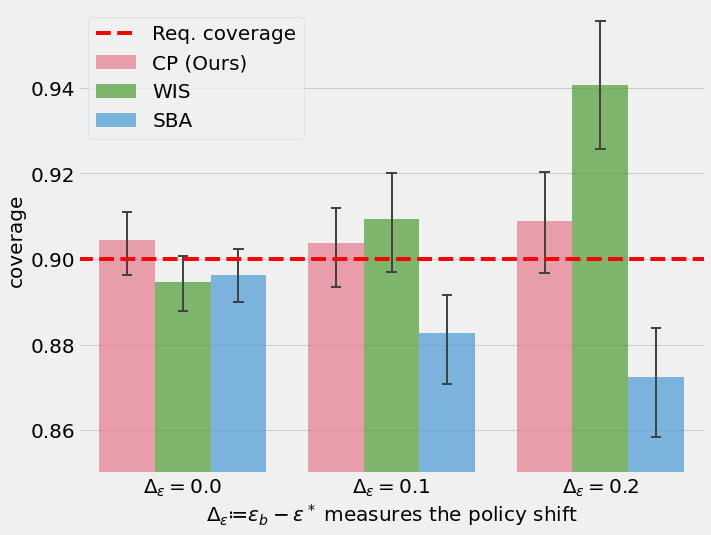
\includegraphics[height=0.8\textwidth, width=0.98\textwidth]{figures/copp/cov-pols1.png}
%     \subcaption{Coverage against policy shift}
%     \label{fig:policy-shift-toy}
%     \end{subfigure}
%     \begin{subfigure}{0.33\textwidth}
%     \centering
%     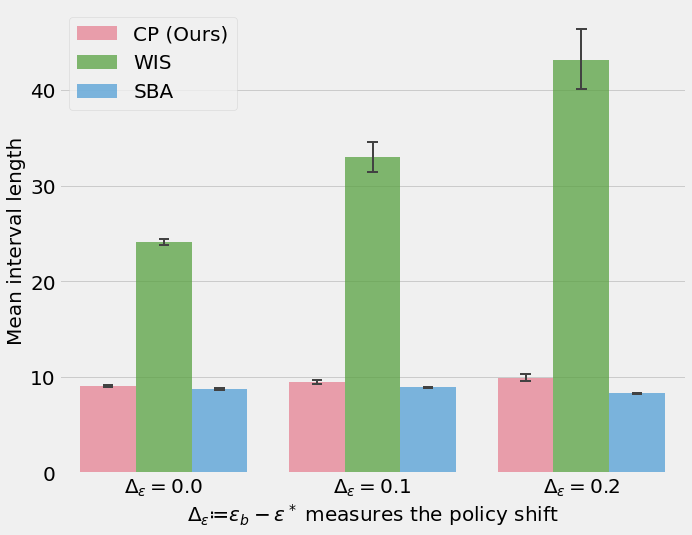
\includegraphics[height=0.8\textwidth, width=0.98\textwidth]{figures/copp/cov-pols-len1.png}
%     \subcaption{Mean Interval lengths against policy shift}
%     \label{fig:policy-shift-len}
%     \end{subfigure}
%     \begin{subfigure}{0.33\textwidth}
%     \centering
%     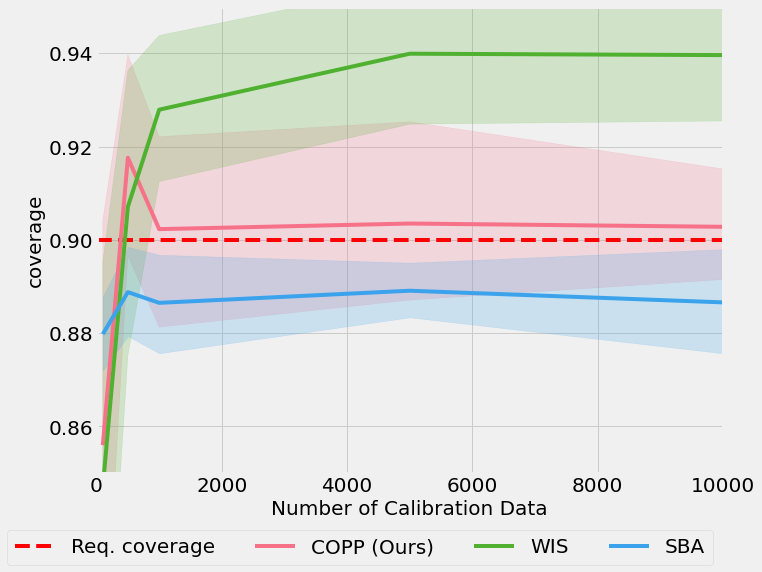
\includegraphics[height=0.8\textwidth, width=0.98\textwidth]{figures/copp/cov-n_cal.png}
%     \subcaption{Coverages against $n$}
%     \label{fig:n_cal}
%     \end{subfigure}
%     \caption{Results for synthetic data experiment with $\pi^b = \pi_{0.3}$. In figures \ref{fig:policy-shift-toy} and \ref{fig:policy-shift-len}, we consider different target policies, $\pi^* \in \{\pi_{0.1}, \pi_{0.2}, \pi_{0.3}\}$ and 5000 calibration data points. In figure \ref{fig:n_cal}, the target policy is $\pi^* = \pi_{0.1}$.}
%     \label{fig:Toy_GT}
% \end{figure*}

\textbf{Estimation of ratios, $\hat{w}(x, y)$.}
Using the training dataset $\mathcal{D}_{tr}$, we estimate $P(y | x, a)$ as $\hat{P}(y | x, a) = \mathcal{N}(\mu(x, a), \sigma(x, a))$, where $\mu(x, a), \sigma(x, a)$ are both neural networks (NNs). Similarly, we use NNs to estimate the behaviour policy $\hat{\pi}^b$ from $\mathcal{D}_{tr}$. Next, to estimate $\hat{w}(x, y)$, we use \eqref{weight-est} with $h = 500$.

\textbf{Score.}
For the score function, we use the same formulation as in \cite{romano2019conformalized}, i.e. $s(x, y) = \max\{ \hat{q}_{\alpha_{lo}}(x) - y, y - \hat{q}_{\alpha_{hi}}(x) \}$, where $\hat{q}_\beta(x)$ denotes the $\beta$ quantile estimate of $P^{\pi^b}_{Y\mid X=x}$ trained using pinball loss.

Lastly, our weights $w(x, y)$ depend on $x$ \textbf{and} $y$ and hence we use a grid of $100$ equally spaced out $y$'s in our experiments to determine the predictive interval which satisfies $\hat{C}_n(x) \coloneqq \{y: s(x,y) \leq \text{Quantile}_{1-\alpha}(\hat{F}_{n}^{x, y})\}$. This is parallelizable and hence does not add much computational overhead.

\textbf{Results.} Table \ref{tab:coverage_toy} shows the coverages of different methods as the policy shift $\Delta_{\epsilon}=\epsilon^b - \epsilon^*$ increases. The behaviour policy $\pi^b = \pi_{0.3}$ is fixed and we use $n=5000$ calibration datapoints, across 10 runs. Table \ref{tab:coverage_toy} shows, how COPP stays very close to the required coverage of $90\%$ across all target policies compared to WIS and SBA. WIS intervals are overly conservative i.e. above the required coverage, while the SBA intervals suffer from under-coverage i.e. below the required coverage. These results supports our hypothesis from Sec. \ref{sec:weights}, which stated that COPP is less sensitive to estimation errors of $\hat{P}(y|x, a)$ compared to directly using $\hat{P}(y|x, a)$ for the intervals, i.e. SBA. 

Next, Table \ref{tab:length_toy} shows the mean interval lengths and even though WIS has reasonable coverage for $\Delta_{\epsilon}=0.0$ and $0.1$, the average interval length is huge compared to COPP. Fig. \ref{fig:copp}b shows the predictive intervals for one such experiment with $\pi^* = \pi_{0.1}$ and $\pi^b = \pi_{0.3}$. We can see that SBA intervals are overly optimistic, while WIS intervals are too wide and are not adaptive w.r.t. $X$. COPP produces intervals which are much closer to the oracle intervals. 

\subsubsection{Ablation Study.} 

To isolate the effect of weight estimation error and policy shift, we conduct an ablation study, comparing COPP with estimated weights to COPP with Ground Truth (GT) weights and standard CP (assuming no policy shift). Table \ref{tab:coverage_toy} shows that at $\Delta_\epsilon = 0$, i.e. no policy shift, standard CP achieves the required coverage as expected. However the coverage of standard CP intervals decreases as the policy shift $\Delta_\epsilon$ increases. COPP, on the other hand, attains the required coverage of $90\%$, by adapting the predictive intervals with increasing policy shift. Table \ref{tab:length_toy} shows that the average interval length of COPP increases with increasing policy shift $\Delta_\epsilon$. Furthermore, Table \ref{tab:coverage_toy} illustrates that while COPP achieves the required coverage for different target policies, on average it is slightly more conservative than using COPP with GT weights. This can be explained by the estimation error in $\hat{w}(x,y)$. Additionally, to investigate the effect of integrating out the actions in \eqref{weight-est}, we also perform CP for each action $a$ separately (as in \cite{lei2020conformal}) and then take the union of the intervals across these actions. In the union method, the probability of an action being chosen is not taken into account, (i.e., intervals are independent of $\pi^*$) and hence the coverage is overly conservative as expected.


% The union method is overall too conservative, and is independent of the target policy, since the probability of an action being chosen is not taken into account when taking the union.

Lastly, we investigate how increasing the number of calibration data $n$ affects the coverage for all the methodologies. We observe that coverage of COPP is closer to the required coverage of $90\%$ compared to the competing methodologies. Additionally, the coverage of COPP converges to the required coverage as $n$ increases; see Appendix \ref{app:N-cal_exp_toy} for detailed experimental results.

% Table \ref{tab:coverage_toy}  shows that when target policy $\pi^* = \pi_{0.1}$, disregarding the policy shift leads to predictive intervals which are under-covered regardless of the number of calibration data. On the other hand, both, our methodology and CP with GT weights converges to required coverage even with 500 calibration data. One important thing to note is the smaller variance of coverage results when using GT weights, as compared to our method, as the estimation of $\hat{w}(x, y)$ adds to the variance in terms of estimation error. 
% \begin{figure*}[t]
%     \begin{subfigure}{0.33\textwidth}
%     \centering
%     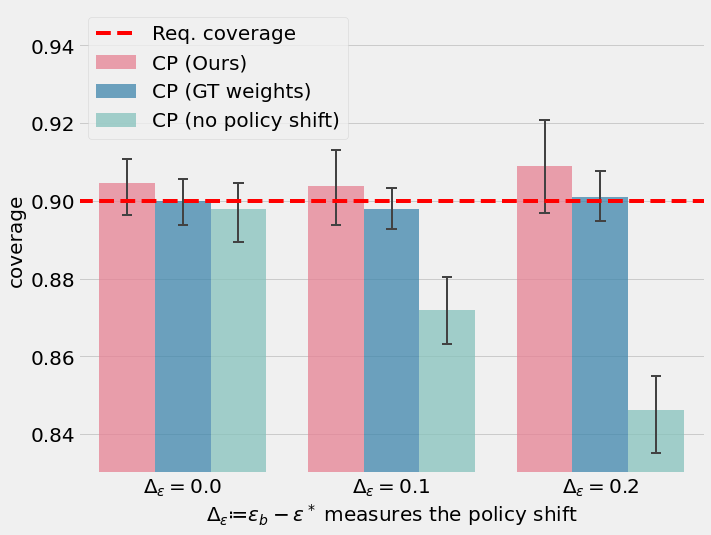
\includegraphics[height=0.8\textwidth, width=0.98\textwidth]{figures/copp/cov-pols-abl1.png}
%     \subcaption{Coverage against policy shift}
%     \label{fig:policy-shift-abl}
%     \end{subfigure}
%     \begin{subfigure}{0.33\textwidth}
%     \centering
%     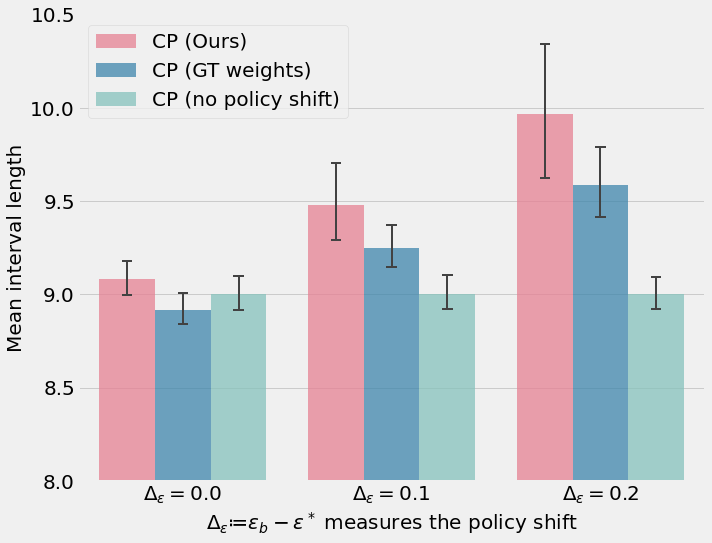
\includegraphics[height=0.8\textwidth, width=0.98\textwidth]{figures/copp/cov-lens-abl1.png}
%     \subcaption{Mean Interval lengths against policy shift} %$\pi^* \in \{\pi_{0.1}, \pi_{0.2}, \pi_{0.3}\}$}
%     \label{fig:policy-shift-len-abl}
%     \end{subfigure}
%     \begin{subfigure}{0.33\textwidth}
%     \centering
%     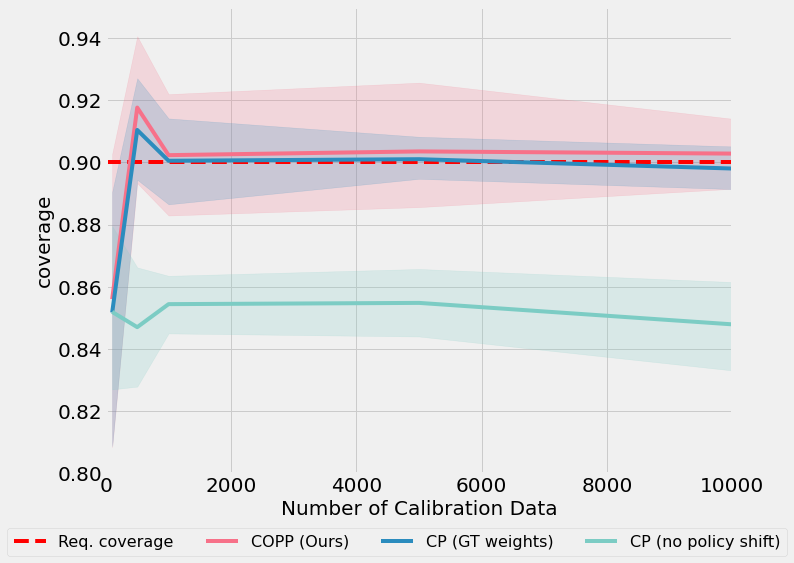
\includegraphics[height=0.8\textwidth, width=0.98\textwidth]{figures/copp/cov-n_cal-abl.png}
%     \subcaption{Coverage against $n$ with $\pi^* = \pi_{0.1}$}
%     \label{fig:ncal-abl}
%     \end{subfigure}
%     \caption{Ablation study results with $\pi^b = \pi_{0.3}$. In figures \ref{fig:policy-shift-abl} and \ref{fig:policy-shift-len-abl}, we consider different target policies, $\pi^* \in \{\pi_{0.1}, \pi_{0.2}, \pi_{0.3}\}$ and $n=5000$. In figure \ref{fig:ncal-abl}, the target policy is $\pi^* = \pi_{0.1}$.}
%     \label{fig:abl}
% \end{figure*}

\begin{table}[t]
\centering
\caption{Mean Coverage as a function of policy shift $\Delta_\epsilon$ and 2 standard errors over 10 runs. COPP attains the required coverage of $90\%$, whereas the competing methods, WIS and SBA, are over-conservative i.e. coverage above $90\%$. In addition, when we do not account for the policy shift, standard CP becomes progressively worse with increasing policy shift.}\label{tab:MSR}
\resizebox{0.7\columnwidth}{!}{%
\begin{tabular}{lccccc}
\toprule
 &  $\Delta_{\epsilon}=0.0$ &  $\Delta_{\epsilon}=0.1$ &  $\Delta_{\epsilon}=0.2$ &  $\Delta_{\epsilon}=0.3$ &  $\Delta_{\epsilon}=0.4$ \\
\midrule
COPP (Ours)            &                  \textbf{0.90 $\pm$ 0.00}&                  \textbf{0.90 $\pm$ 0.02}&                  \textbf{0.90 $\pm$ 0.01}&                  \textbf{0.89 $\pm$ 0.01}&                  \textbf{0.91 $\pm$ 0.01}\\
WIS                  &                  1.00 $\pm$ 0.00&                  1.00 $\pm$ 0.00&                  0.92 $\pm$ 0.00&                  0.94 $\pm$ 0.00&                  0.91 $\pm$ 0.00\\
SBA                  &                  0.99 $\pm$ 0.00&                  0.99 $\pm$ 0.00&                  0.98 $\pm$ 0.00&                  0.97 $\pm$ 0.00&                  0.96 $\pm$ 0.00\\
\midrule
\midrule
% CP (GT behav policy) &                  0.95 $\pm$ 0.10&                 \textbf{ 0.90 $\pm$ 0.02}&                  \textbf{0.90 $\pm$ 0.01}&                  \textbf{0.89 $\pm$ 0.01}&                  \textbf{0.91 $\pm$ 0.01}\\
CP (no policy shift) &                  \textbf{0.91 $\pm$ 0.02}&                 \textbf{ 0.92 $\pm$ 0.02}&                  0.93 $\pm$ 0.01&                  0.94 $\pm$ 0.01&                  0.96 $\pm$ 0.01\\
\bottomrule
\end{tabular}%
}
\end{table}


\subsection{Experiments on Microsoft Ranking Dataset}

We now apply COPP onto a real dataset i.e. the Microsoft Ranking dataset 30k \citep{msr, swaminathan2016off, bietti2018contextual}. Due to space constraints, we have added additional extensive experiments on UCI datasets in Appendix \ref{sec:UCI}.


\textbf{Dataset.}
% The dataset contains relevance scores for websites recommended to different users, and comprises of $30,000$ user-website pairs. For a user $i$ and website $j$, the data contains a $136$-dimensional feature vector $u_i^j$, which consists of user $i$'s attributes corresponding to website $j$, such as length of stay or number of clicks on the website. Furthermore, for each user-website pair, the dataset also contains a relevance score, i.e. how relevant the website was to the user.
The dataset contains relevance scores for websites recommended to different users, and comprises of $30,000$ user-website pairs. For each user-website pair, the data contains a $136$-dimensional feature vector, which consists of user's attributes corresponding to the website, such as length of stay or number of clicks on the website. Furthermore, for each user-website pair, the dataset also contains a relevance score, i.e. how relevant the website was to the user.

% First, given a user $i$ we sample (with replacement) $5$ websites,  $\{u_i^j\}_{j=1}^5$, from the data. Next, we reformulate this into a contextual bandit where $A \in \{1,2,3,4,5\}$ corresponds to the website we recommend to a user. For a user $i$, we define $X$ by combining the $5$ feature vectors corresponding to the user, i.e. $X \in \mathbb{R}^{5 \times 136}$, where $x_i = (u^1_{i},u^2_{i},u^3_{i},u^4_{i}, u^5_{i})$. In addition, $Y \in\{0,1,2,3,4\}$ corresponds to the relevance score for the $A$'th website, i.e. the recommended website. The goal is to construct prediction sets that are guaranteed to contain the true relevance score with a probability of $90\%$.

First, given a user, we sample (with replacement) $5$ websites from the data corresponding to that user. Next, we reformulate this into a contextual bandit where $a_i \in \{1,2,3,4,5\}$ corresponds to the action of recommending the $a_i$'th website to the user $i$. $x_i$ is obtained by combining the $5$ user-website feature vectors corresponding to the user $i$ i.e. $x_i \in \mathbb{R}^{5 \times 136}$. $y_i \in\{0,1,2,3,4\}$ corresponds to the relevance score for the $a_i$'th website, i.e. the recommended website. The goal is to construct prediction sets that are guaranteed to contain the true relevance score with a probability of $90\%$.

% This problem can be formulated as a contextual bandit by firstly, obtaining some behavioural data, where the action $A \in \{1,2,3,4,5\}$ corresponds to the website we recommend and which has been sampled from $\pi^b(a|x)$. 

% Moreover, given that we want to rank $5$ websites per user, each recommendation task will have a feature vector $X \in \mathbb{R}^{5 \times 136}$, where $x_i = (u^1_{i},u^2_{i},u^3_{i},u^4_{i}, u^5_{i})$. In addition, $Y \in\{0,1,2,3,4\}$ will correspond to the relevance score for the $A$'th website, i.e. the website that was recommended.

% We use $\hat{f}^{\textup{label}}_\theta$ to denote the relevance class predicted by $\hat{f}_\theta$, i.e. $\hat{f}^{\textup{label}}_\theta(u) \coloneqq \argmax_j\{\hat{f}_\theta(u^{j})\}$.


% \begin{align}
%     &\pi_\epsilon (a\mid X=(u^1, u^2,u^3,u^4,u^5)) \coloneqq \nonumber \\ 
%     &\epsilon \mathbbm{1}(a = \argmax_j\{ \hat{f}^{\textup{label}}_\theta(u^j \}) \nonumber \\ 
%     &+ (1-4\epsilon) \mathbbm{1}(a \neq \argmax_j\{ \hat{f}^{\textup{label}}_\theta(u^j) \}) \nonumber
% \end{align}
% The problem being considered in this dataset is somewhat analogous to the one of recommending treatment to patients in the medical setting. Specifically, in both cases we would like to recommend websites/treatments which are relevant to the users/patients and avoid ones which are not. 

\textbf{Behaviour and Target Policies.} 
We first train a NN classifier model, $\hat{f}_\theta$, mapping each 136-dimensional user-website feature vector to the softmax scores for each relevance score class. We use this trained model $\hat{f}_\theta$ to define a family of policies which pick the most relevant website as predicted by $\hat{f}_\theta$ with probability $\epsilon$ and the rest uniformly with probability $(1-\epsilon)/4$ (see Appendix \ref{sec:MSR_experiments_decrip} for more details). Like the previous experiment, we use $\epsilon$ to control the shift between behaviour and target policies. For $\pi^b$, we use $\epsilon^b = 0.5$ and for $\pi^*$, $\epsilon^* \in \{0.1, 0.2, 0.3, 0.4, 0.5\}$. 
% Using this behaviour policy $\pi^b$, we generate an observational dataset $\mathcal{D}_{obs} = \{x_i, a_i, y_i\}_{i=1}^{n_{obs}}$ which is then split into training $\mathcal{D}_{tr}$ and calibration datasets $\mathcal{D}_{cal}$, of sizes $m$ and $n$ respectively.
% We first train a NN classifier model mapping each 136-dimensional feature vector to the softmax scores for each relevance score class, $\hat{f}_\theta:\mathcal{U} \rightarrow [0,1]^5$. We use this trained model $\hat{f}_\theta$ to define a family of policies which pick the most relevant website as predicted by $\hat{f}_\theta$ with probability $\epsilon$ and the rest uniformly with probability $(1-\epsilon)/4$ (see \ref{sec:MSR_experiments_decrip} for more details). Like the previous experiment, we use $\epsilon$ to control the shift between behaviour and target policies. For $\pi^b$, we use $\epsilon^b = 0.5$ and for $\pi^*$, $\epsilon^* \in \{0.1, 0.2, 0.3, 0.4, 0.5\}$. Using this behaviour policy $\pi^b$, we generate an observational dataset $\mathcal{D}_{obs} = \{x_i, a_i, y_i\}_{i=1}^{n_{obs}}$ which is then split into training $\mathcal{D}_{tr}$ and calibration datasets $\mathcal{D}_{cal}$, of sizes $m$ and $n$ respectively.

\textbf{Estimation of ratios $\hat{w}(X, Y)$.}
To estimate the $\hat{P}(y \mid x, a)$ we use the trained model $\hat{f}_\theta$ as detailed in Appendix \ref{sec:MSR_experiments_decrip}. To estimate the behaviour policy $\hat{\pi}^b$, we train a neural network classifier model $\mathcal{X} \rightarrow \mathcal{A}$, and we use \eqref{weight-est} to estimate the weights $\hat{w}(x, y)$.
% To estimate the $\hat{P}(y \mid x, a)$ we use the trained model $\hat{f}_\theta$ as follows:
% \[
% \hat{P}(y \mid x = (u^1, u^2,u^3,u^4,u^5), a) = \hat{f}_\theta(u^a)_y
% \]
% where $\hat{f}_\theta(u^a)_y$ corresponds to the softmax prediction of $u^a$ for label $y$ under the model $\hat{f}_\theta$. To estimate the behaviour policy $\hat{\pi}^b$, we train a classifier model $\mathcal{X} \rightarrow \mathcal{A}$ using a neural network. We use \eqref{weight-est} to estimate the weights $\hat{w}(x, y)$.

\textbf{Score.} The space of outcomes $\mathcal{Y}$ in this experiment is discrete. We define $\hat{P}^{\pi^b}(y \mid x) = \sum_{i = 1}^5 \hat{\pi}^b(A = i|x) \hat{P}(y|x, A = i)$. Using similar formulation as in \cite{conf-bates}, we define the score:
$$
s(x, y) = \sum_{y' = 0}^4 \hat{P}^{\pi^b}(y' \mid x) \mathbbm{1}(\hat{P}^{\pi^b}(y' \mid x) \geq \hat{P}^{\pi^b}(y \mid x)).
$$
Since $\mathcal{Y}$ is discrete, we no longer need to construct a grid of $y$ values on which to compute $\text{Quantile}_{1-\alpha}(\hat{F}_{n}^{x, y})$. Instead, we will simply compute this quantity on each $y \in \mathcal{Y}$, when constructing the predictive sets $\hat{C}_{n}(x^{test})$.

% \begin{figure*}[t]
%     \begin{subfigure}{0.5\textwidth}
%     \centering
%     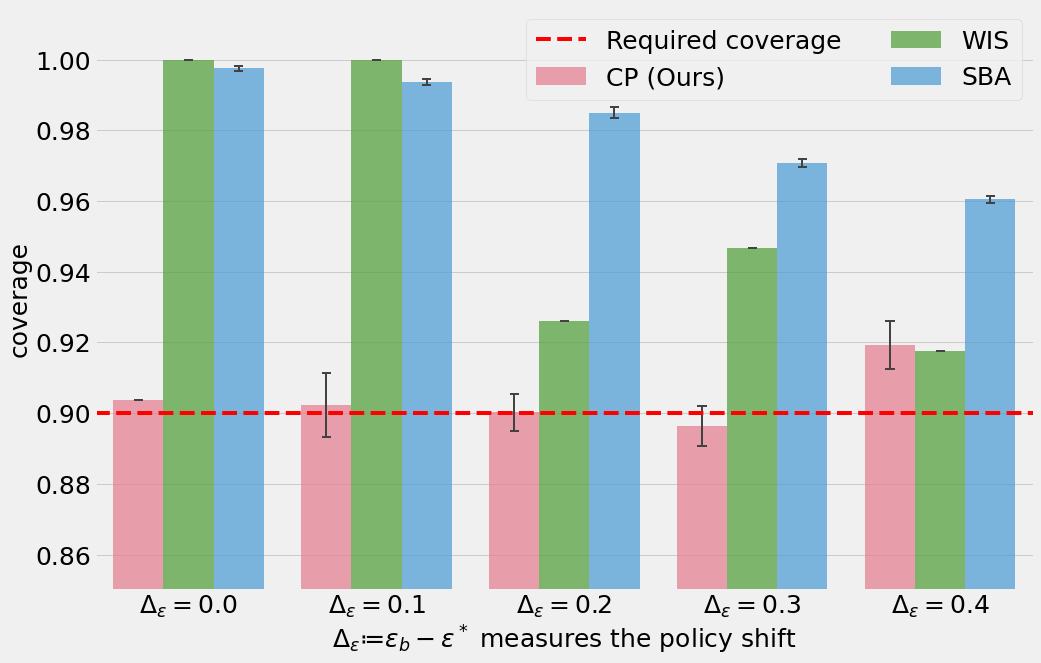
\includegraphics[height=0.6\textwidth]{figures/copp/cov-pols-msr.png}
%     \subcaption{Coverage against policy shift}
%     \label{fig:policy-shift-msr}
%     \end{subfigure}
%     \begin{subfigure}{0.5\textwidth}
%     \centering
%     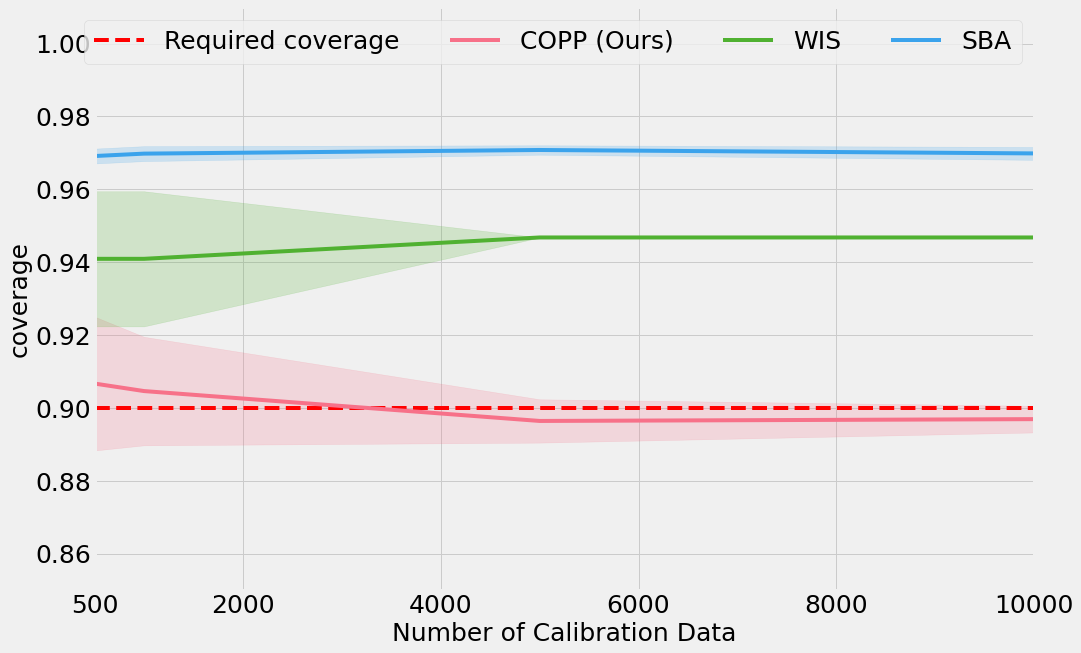
\includegraphics[height=0.6\textwidth]{figures/copp/cov-ncal-msr.png}
%     \subcaption{Coverage against $n$} %$\pi^* \in \{\pi_{0.1}, \pi_{0.2}, \pi_{0.3}\}$}
%     \label{fig:ncal-msr}
%     \end{subfigure}
%     \caption{Results of Microsoft Ranking Dataset experiment with behaviour policy $\pi^b = \pi_{0.5}$. In figure \ref{fig:policy-shift-msr}, we consider different target policies, $\pi^* \in \{\pi_{0.1}, \pi_{0.2}, \dots, \pi_{0.5} \}$ and $n=5000$. In figure \ref{fig:ncal-msr}, the target policy is $\pi^* = \pi_{0.2}$.}
%     \label{fig:msr}
% \end{figure*}

\textbf{Results.}
% Here below, we can see the coverage plots when using our proposed methods standard classification and \cite{risk-assessment}. We can see from the below plots that our proposed method is able to attain the required coverage consistently, whereas \cite{risk-assessment} is over-conservative. Lastly, if we do not use the conformal prediction framework, we can see from Fig.[ref] that we can no longer guarantee coverage and suffer from under-coverage.
Table \ref{tab:MSR} shows the coverages of different methodologies across varying target policies $\pi_{\epsilon^*}$. The behaviour policy $\pi^b = \pi_{0.5}$ is fixed and we use $n=5000$ calibration datapoints, across 10 runs. Table \ref{tab:MSR} also shows that the coverage of WIS and SBA sets is dependent upon the policy shift, with both being overly conservative across the different target policies as compared to COPP. Recall that the WIS sets do not depend on $x^{test}$ and as a result we get the same set for each test data point. This becomes even more problematic when $Y$ is discrete -- if, for each label $y$, $\tarprob(Y = y)>10\%$, then WIS sets (with the required coverage of $90\%$) are likely to contain every label $y \in \mathcal{Y}$.
% This becomes even more problematic when $Y$ is discrete as there are finitely many possible sets that can be constructed, and consequently the achieved coverage cannot be arbitrarily close to the required coverage. In particular, when $\epsilon^b=0.5$, small $\Delta_{\epsilon}$ values indicate that the target policy is well spread out with each action having at least $10\%$ probability. Hence if we would like to achieve marginal coverage of at least $90\%$, we need to include all the labels, give that the intervals are not dependent on $x$ for WIS. 
In comparison, COPP is able to stay much closer to the required coverage of $90\%$ across all target policies. We have also added standard CP without policy shift as a sanity check, and observed that the sets get increasingly conservative as the policy shift increases.

% for the target policy $\pi^* = \pi_{0.2}$ evolves 
Finally, we also plotted how the coverage changes as the number of calibration data $n$ increases. We observe again that the coverage of COPP is closer to the required coverage of $90\%$ compared to the competing methodologies. Due to space constraints, we have added the plots in Appendix \ref{app:N-cal_exp_msr}.

% Moreover, we observe that our method only requires around $500$ calibration data to obtain the required coverage, and that it converges to the required $90\%$ as the number of calibration data increases. Both, SBA and WIS on the other hand remain overly conservative even with increasing calibration data. 

% Note that we only we only included the high number of calibration data to check convergence and do not expect to have this amount of calibration data in practice.

\textbf{Class-balanced conformal prediction.}
Using the methodology described in Sec. \ref{sec:group_balanced_cov}, we construct predictive sets, $\hat{C}^{\mathcal{Y}}_n(x)$, which offer label conditioned coverage guarantees (see \ref{sec:grp-bal}), i.e. for all $y\in \mathcal{Y}$, 
$$
\tarprob(Y \in \hat{C}^{\mathcal{Y}}_n(X) \mid Y = y) \geq 1- \alpha.
$$
We empirically demonstrate that $\hat{C}^{\mathcal{Y}}_n$ provides label conditional coverage, while $\hat{C}_n$ obtained using alg. \ref{cp_covariate_shift} may not. Due to space constraints, details on construction of $\hat{C}^{\mathcal{Y}}_n$ as well as experimental results have been included in Appendix \ref{sec:results_class_bal_coverage}.

\section{Conclusion and Limitations}\label{sec:lims}

% In this paper, we construct predictive intervals for contextual bandits to assess a target policy $\pi^*$ given observational data generated from a behavioural policy $\pi^b$. 
In this paper, we propose COPP, an algorithm for constructing predictive intervals on off-policy outcomes, which are adaptive w.r.t. covariates $X$. We theoretically prove that COPP can guarantee finite-sample coverage by adapting the framework of conformal prediction to our setup.
Our experiments show that conventional methods cannot guarantee any user pre-specified coverage, whereas COPP can.
For future work, it would be interesting to apply COPP to policy training. This could be a step towards robust policy learning by optimising the worst case outcome \citep{stutz2021learning}.

We conclude by mentioning several limitations of COPP. 
Firstly, we do not guarantee conditional coverage in general.
We outline conditions under which conditional coverage holds asymptotically (Prop. \ref{conditional-res}), however, this relies on somewhat strong assumptions.
Secondly, our current method estimates the weights $w(x, y)$ through $P(y \mid x, a)$, which can be challenging.
We address this limitation in Appendix \ref{sec:alternate_weights_est}, where we propose an alternative method to estimate the weights directly, without having to model $P(y \mid x, a)$. % We leave this avenue for future work. 
Lastly, reliable estimation of our weights $\hat{w}(x, y)$ requires sufficient overlap between behaviour and target policies. The results from COPP may suffer in cases where this assumption is violated, which we illustrate empirically in Appendix \ref{subsec:cts_act}.
% We leave further consideration of how to address these limitations to future work.
We believe these limitations suggest interesting research questions that we leave to future work.

% Moreover, in this paper we have not considered the case where both the marginal in $X$ and the conditional shift, which is a straightforward extension of COPP, as the theory only relies on the ratio of the joint distribution. We leave this for future work.


\section*{Acknowledgements}
We would like to thank Andrew Jesson, Sahra Ghalebikesabi, Robert Hu, Siu Lun Chau and Tim Rudner for useful feedback.
JFT is supported by the EPSRC and MRC through the OxWaSP CDT programme (EP/L016710/1).
MFT acknowledges his PhD funding from Google DeepMind.
RC and AD are supported by the Engineering and Physical Sciences Research Council (EPSRC) through the Bayes4Health programme [Grant number EP/R018561/1].  

% \bibliographystyle{abbrv}

%%%%%%%%%%%%%%%%%%%%%%%%%%%%%%%%%%%%%%%%%%%%%%%%%%%%%%%%%%%%

\begin{comment}


\section*{Checklist}


%%% BEGIN INSTRUCTIONS %%%
% The checklist follows the references.  Please
% read the checklist guidelines carefully for information on how to answer these
% questions.  For each question, change the default \answerTODO{} to \answerYes{},
% \answerNo{}, or \answerNA{}.  You are strongly encouraged to include a {\bf
% justification to your answer}, either by referencing the appropriate section of
% your paper or providing a brief inline description.  For example:
% \begin{itemize}
%   \item Did you include the license to the code and datasets? \answerYes{See Section~\ref{gen_inst}.}
%   \item Did you include the license to the code and datasets? \answerNo{The code and the data are proprietary.}
%   \item Did you include the license to the code and datasets? \answerNA{}
% \end{itemize}
% Please do not modify the questions and only use the provided macros for your
% answers.  Note that the Checklist section does not count towards the page
% limit.  In your paper, please delete this instructions block and only keep the
% Checklist section heading above along with the questions/answers below.
%%% END INSTRUCTIONS %%%


\begin{enumerate}


\item For all authors...
\begin{enumerate}
  \item Do the main claims made in the abstract and introduction accurately reflect the paper's contributions and scope?
    \answerYes{}
  \item Did you describe the limitations of your work?
    \answerYes{} See section \ref{sec:lims}.
  \item Did you discuss any potential negative societal impacts of your work?
    \answerNA{}
  \item Have you read the ethics review guidelines and ensured that your paper conforms to them?
    \answerYes{}
\end{enumerate}


\item If you are including theoretical results...
\begin{enumerate}
  \item Did you state the full set of assumptions of all theoretical results?
    \answerYes{} See section \ref{sec:theory}.
        \item Did you include complete proofs of all theoretical results?
    \answerYes{} See section \ref{sec:proofs}.
\end{enumerate}


\item If you ran experiments...
\begin{enumerate}
  \item Did you include the code, data, and instructions needed to reproduce the main experimental results (either in the supplemental material or as a URL)?
    \answerYes{} See section \ref{sec:exps_app}.
  \item Did you specify all the training details (e.g., data splits, hyperparameters, how they were chosen)?
    \answerYes{} See sections \ref{sec:exp}, \ref{sec:exps_app}.
        \item Did you report error bars (e.g., with respect to the random seed after running experiments multiple times)?
    \answerYes{} See sections \ref{sec:exp}, \ref{sec:exps_app}.
        \item Did you include the total amount of compute and the type of resources used (e.g., type of GPUs, internal cluster, or cloud provider)?
    \answerYes{}See section \ref{sec:exps_app}.
\end{enumerate}


\item If you are using existing assets (e.g., code, data, models) or curating/releasing new assets...
\begin{enumerate}
  \item If your work uses existing assets, did you cite the creators?
    \answerNA{}
  \item Did you mention the license of the assets?
    \answerNA{}
  \item Did you include any new assets either in the supplemental material or as a URL?
    \answerNA{}
  \item Did you discuss whether and how consent was obtained from people whose data you're using/curating?
    \answerNA{}
  \item Did you discuss whether the data you are using/curating contains personally identifiable information or offensive content?
    \answerNA{}
\end{enumerate}


\item If you used crowdsourcing or conducted research with human subjects...
\begin{enumerate}
  \item Did you include the full text of instructions given to participants and screenshots, if applicable?
    \answerNA{}
  \item Did you describe any potential participant risks, with links to Institutional Review Board (IRB) approvals, if applicable?
    \answerNA{}
  \item Did you include the estimated hourly wage paid to participants and the total amount spent on participant compensation?
    \answerNA{}
\end{enumerate}


\end{enumerate}
\end{comment}

%%%%%%%%%%%%%%%%%%%%%%%%%%%%%%%%%%%%%%%%%%%%%%%%%%%%%%%%%%%%
\newpage



\ifthenelse{\boolean{compilePapers}}
    { % If compilePapers is true, this block will be executed
        
% \usepackage[utf8]{inputenc} % allow utf-8 input
% \usepackage[T1]{fontenc}    % use 8-bit T1 fonts
% \usepackage[hidelinks]{hyperref}% hyperlinks
% \usepackage{url}            % simple URL typesetting
% \usepackage{booktabs}       % professional-quality tables
% \usepackage{amsfonts}       % blackboard math symbols
% \usepackage{nicefrac}       % compact symbols for 1/2, etc.
% \usepackage{microtype}      % microtypography
% \usepackage{xcolor}         % colors

% \usepackage{lipsum}

% \newcommand\blfootnote[1]{%
%   \begingroup
%   \renewcommand\thefootnote{}\footnote{#1}%
%   \addtocounter{footnote}{-1}%
%   \endgroup
% }



% \title{Conformal Off-Policy Prediction in Contextual Bandits}


% The \author macro works with any number of authors. There are two commands
% used to separate the names and addresses of multiple authors: \And and \AND.
%
% Using \And between authors leaves it to LaTeX to determine where to break the
% lines. Using \AND forces a line break at that point. So, if LaTeX puts 3 of 4
% authors names on the first line, and the last on the second line, try using
% \AND instead of \And before the third author name.

% \author[1]{Muhammad Faaiz Taufiq*} 
% \author[2]{Jean-Fran\c cois Ton*} 
% \author[1]{Rob Cornish} 
% \author[1]{Yee Whye Teh} 
% \author[1]{Arnaud Doucet} 

% \affil[1]{Department of Statistics, University of Oxford}
% \affil[2]{ByteDance Research}

% \author{%
%   Muhammad Faaiz Taufiq* \\
%   Department of Statistics\\
%   University of Oxford\\
%   % examples of more authors
%    \And
%    Jean-Francois Ton*$^\dagger$ \\
%    AI-Lab-Research\\
%    Bytedance AI Lab \\
%    \AND
%    Rob Cornish \\
%    Department of Statistics \\
%    University of Oxford\\
%    \And
%    Yee Whye Teh \\
%    Department of Statistics \\
%    University of Oxford\\
%    \And
%    Arnaud Doucet \\
%    Department of Statistics \\
%    University of Oxford\\
% }



\begin{abstract}
  Most off-policy evaluation methods for contextual bandits have focused on the expected outcome of a policy, which is estimated via methods that at best provide only asymptotic guarantees. However, in many applications, the expectation may not be the best measure of performance as it does not capture the variability of the outcome. In addition, particularly in safety-critical settings, stronger guarantees than asymptotic correctness may be required. To address these limitations, we consider a novel application of conformal prediction to contextual bandits. Given data collected under a behavioral policy, we propose \emph{conformal off-policy prediction} (COPP), which can output reliable predictive intervals for the outcome under a new target policy. We provide theoretical finite-sample guarantees without making any additional assumptions beyond the standard contextual bandit setup, and empirically demonstrate the utility of COPP compared with existing methods on synthetic and real-world data. 
  % \blfootnote{$^*$Denotes equal contribution, where ordering was determined through coin flip. Corresponding authors \texttt{muhammad.taufiq@stats.ox.ac.uk} and \texttt{jeanfrancois@bytedance.com}.
%   \blfootnote{$\dagger$ Work primarily done at the University of Oxford and finished at Bytedance.}
\end{abstract}

\section{Introduction}
% Often in safety-critical environments such as healthcare, we cannot afford to implement new policies, without reliably evaluating the effectiveness/safety of the policies. In such situations, we must resort to using available observational data to infer outcomes under a new target policy which has not been implemented in the real world. This is known as off-policy evaluation. 


% \R{In domains such as healthcare or recommendation systems, understanding all the possible outcomes is at the core of safe and informed decision making.} Due to ethical or financial constraints, we can often not implement new policies $\pi^*$, without first reliably evaluating its effectiveness and safety. In such cases we have to rely on observational data, which has been collected under a different policy $\pi^b$. Using this data to evaluate a policy $\pi^*$ is known as off-policy evaluation (OPE) and helps us assess $\pi^*$ without having to deploy it.
% % which can be both costly and risky. we use the same formulationas in Romano et al. (2019), i.
% % Hence it is crucial to determine the most likely outcomes under a new policy in a reliable manner.


Before deploying a decision-making policy to production, it is usually important to understand the plausible range of outcomes that it may produce.
However, due to resource or ethical constraints, it is often not possible to obtain this understanding by testing the policy directly in the real-world.
In such cases we have to rely on observational data collected under a different policy than the target.
Using this observational data to evaluate the target policy is known as off-policy evaluation (OPE).% and helps us assess $\pi^*$ without having to deploy it.


% policies $\pi^*$, without first reliably evaluating its effectiveness and safety. In such cases we have to rely on observational data, which has been collected under a different policy $\pi^b$. Using this data to evaluate a policy $\pi^*$ is known as off-policy evaluation (OPE) and helps us assess $\pi^*$ without having to deploy it.

% To make safe and informed decisions, it is important to understand the range of plausible outcomes that may occur under the different choices available.


% Due to the tremendous increase in data availability over the years, we often find ourselves in situations where we have an abundance of observational data, i.e. data which has been collected under a certain unknown behaviour policy $\pi^b$ but want to infer outcomes \textit{as if} the data was collected under $\pi^*$. In cases, where a new policy $\pi^*$ is expensive or unethical to implement, we have to rely on the observational data and perform off-policy evaluations (OPE) of $\pi^*$ in order to determine whether the new policy can be safely implemented in the real world. Hence it is crucial to be able to determine the most likely outcomes under a new policy in a reliable manner.
% Due to the popularity of concentration inequalities \cite{concentrationineq} computing bounds on the expectation becomes feasible. 
% 1. Doesn't take into account any notions of variance. 
% 2. Can be highly prone to outliers, especially, when the size of data is small. 
% -> Therefore, often in safety-critical settings, like econometrics, metrics such as VaR (Value at Risk) are used as they are better representations of potential risk. 
% -> instead, in safety-critical settings, where one might be concerned with minimizing potential risk, the distribution of the outcome itself might be more informative. 

Traditionally, most techniques for OPE in contextual bandits focus on evaluating policies based on their \textbf{expected} outcomes; see e.g., \cite{uncertainty5, adaptive-ope, uncertainty2, uncertainty3, uncertainty4, doubly-robust}.
However, this can be problematic as methods that are only concerned with the average outcome do not take into account any notions of variance, for example. Therefore, in risk-sensitive settings such as econometrics, where we want to minimize the potential risks, metrics such as CVaR (Conditional Value at Risk) might be more appropriate \citep{keramati2020being}. Additionally, when only small sample sizes of observational data are available, the average outcomes under finite data can be misleading, as they are prone to outliers and hence, metrics such as medians or quantiles are more robust in these scenarios \citep{altschuler2019best}.

% and hence, predictive bounds based on the outcome distribution instead of the average are more informative. 
% Hence, in high stake settings such as healthcare where medical practitioner are more concerned with minimizing potential risk, knowing high probability bounds of possible outcomes of a new policy is extremely useful, as it allows them to make better informed decisions. In recommendation systems where a vast majority of the data are be outliers, methodologies that focus on the average outcome become misleading and uninformative. 
%  In addition, due to the finite data regime these methods are very susceptible to outliers [refs].
\begin{figure}
     \centering
     \begin{subfigure}[t]{0.5\textwidth}
         \centering
         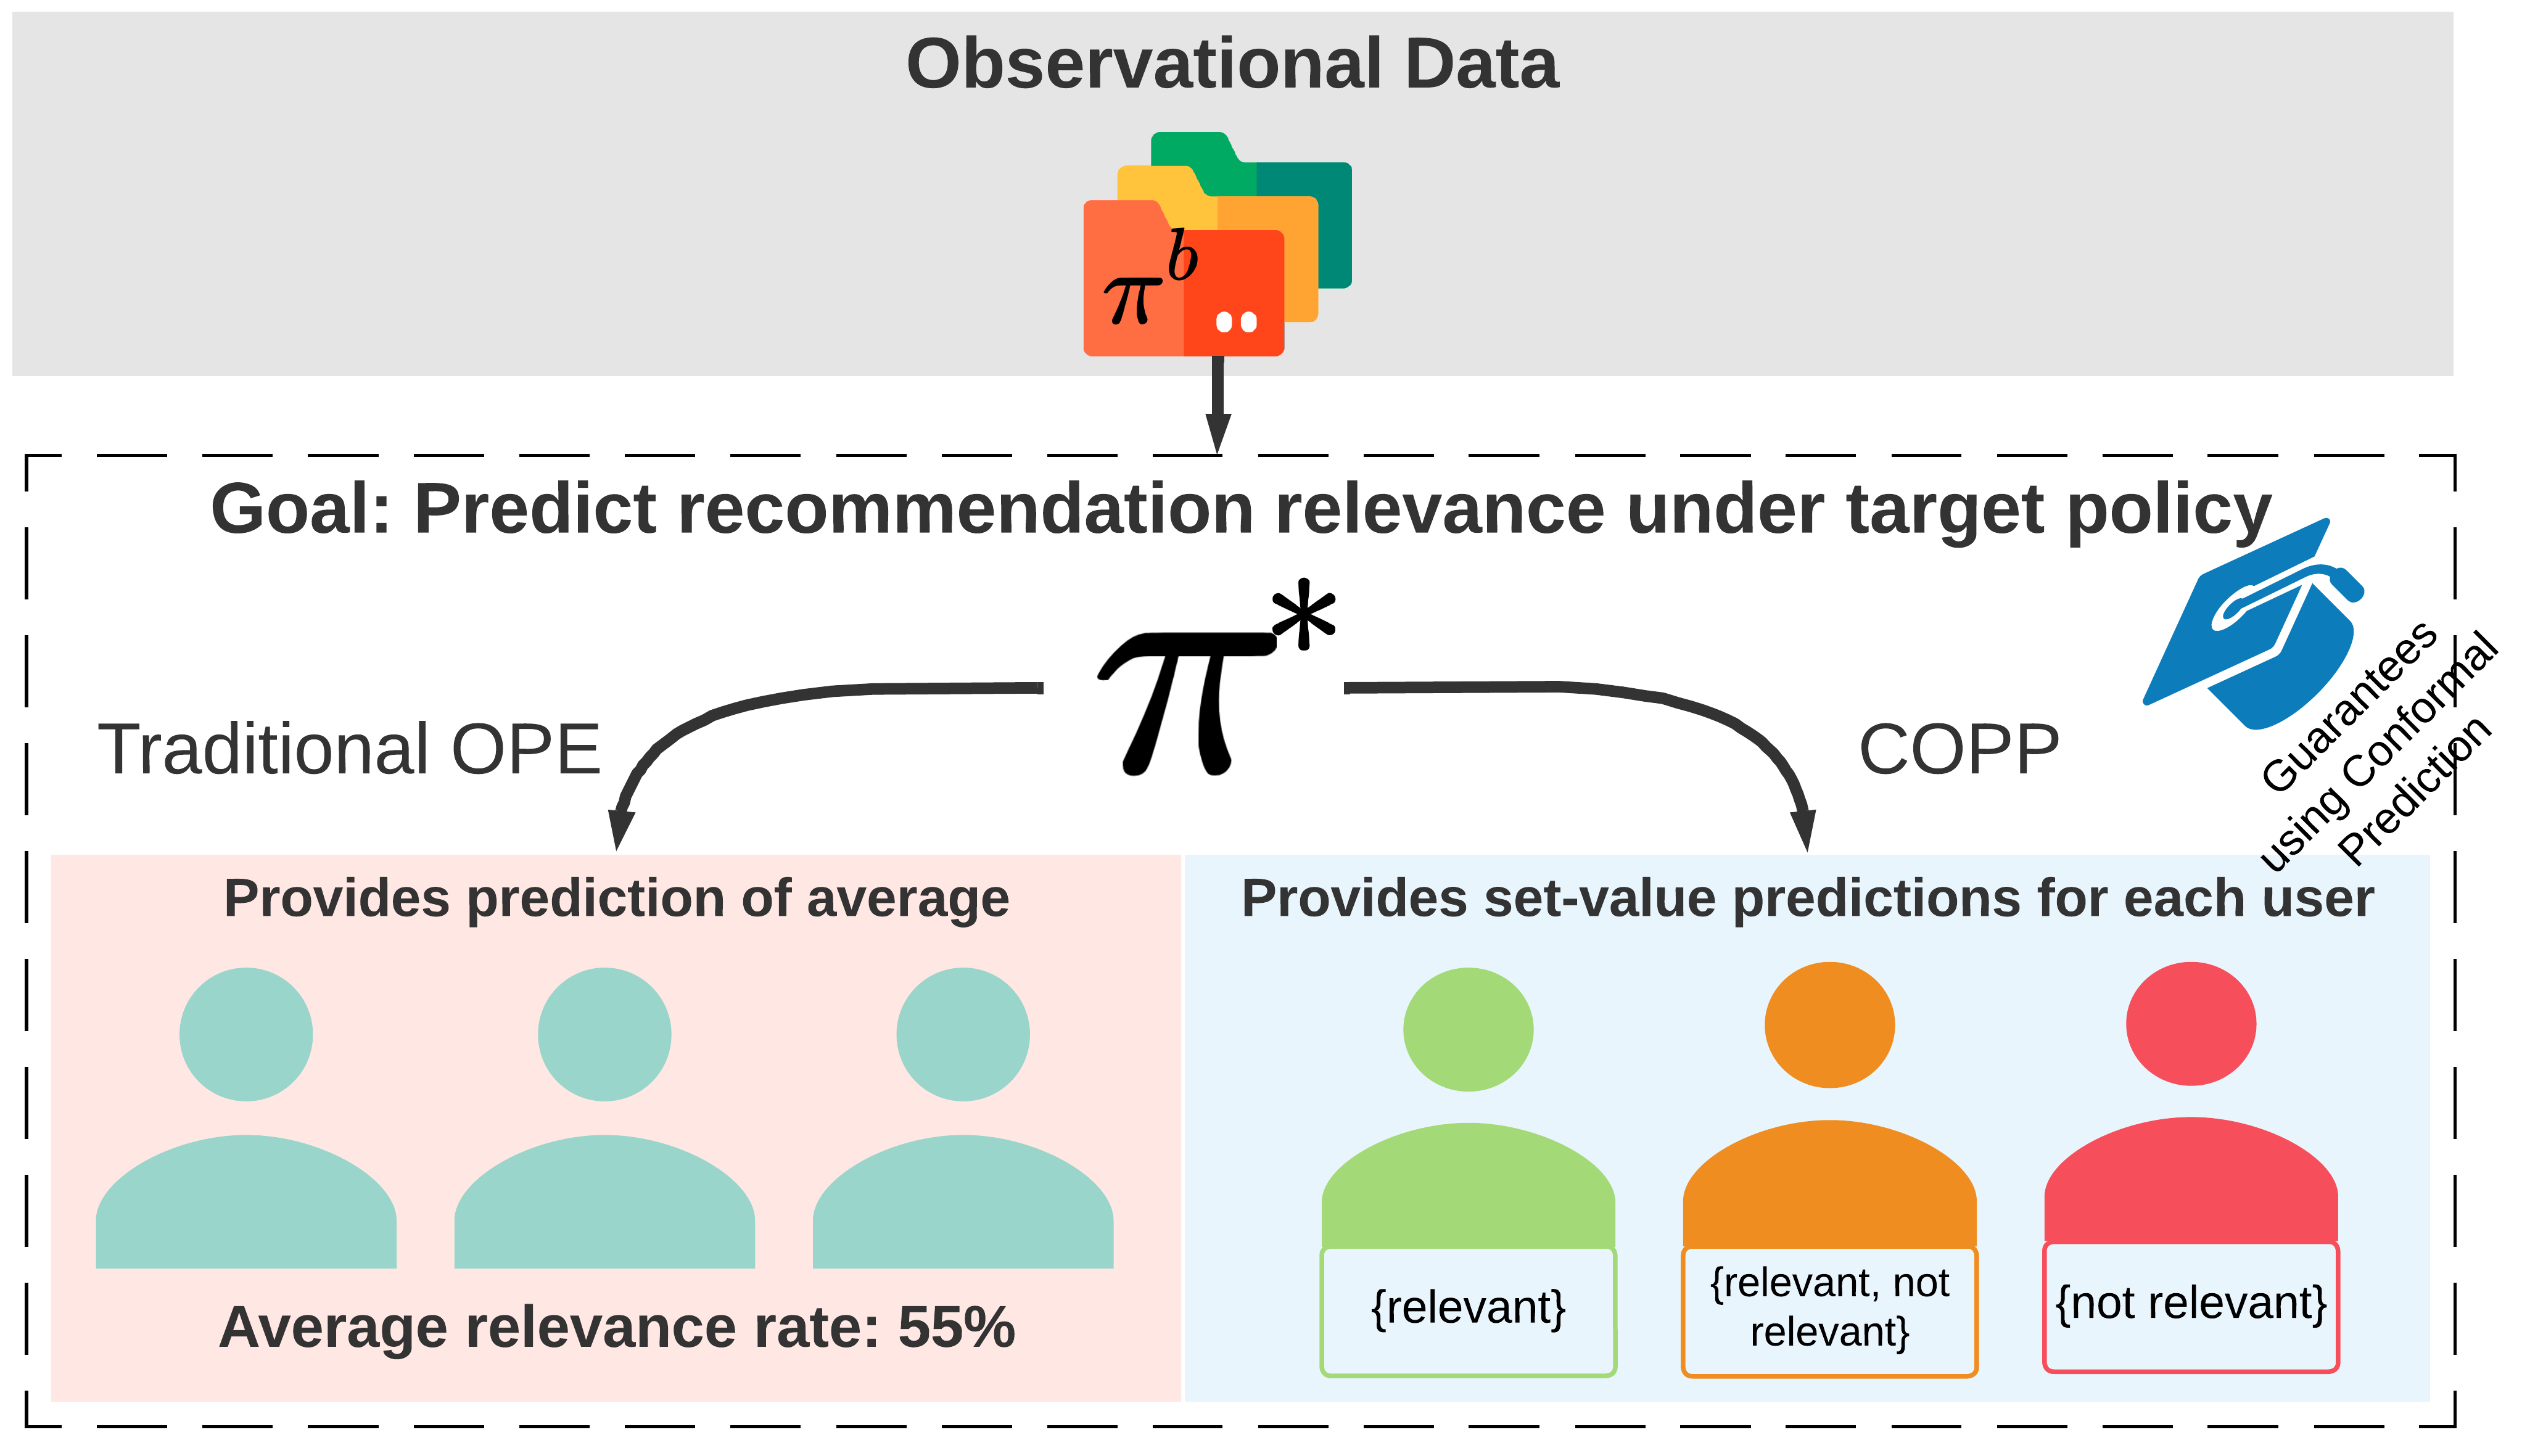
\includegraphics[height=1.85in]{figures/copp/COPP7.png}
        %  \subcaption{Conformal Off-Policy Prediction compared to standard off-policy evaluation methods.}
        %  \label{fig:copp}
     \end{subfigure}%\hspace{0.8cm}%
     \begin{subfigure}[t]{0.5\textwidth}
         \centering
         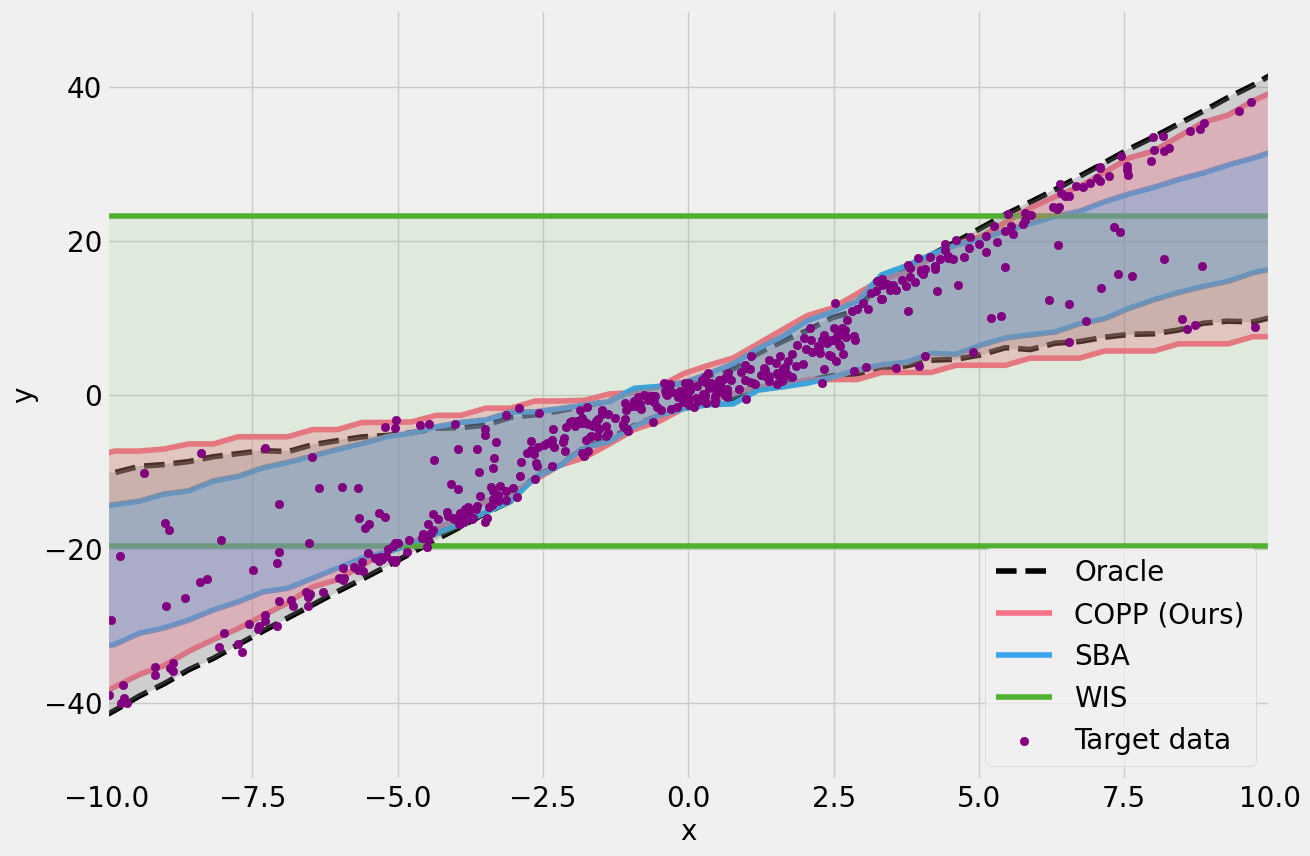
\includegraphics[height=1.85in]{figures/copp/cis-updated.png}
        %  \subcaption{$90\%$ predictive intervals for $Y$ as a function of $X$ for COPP, competing methods and the oracle.}
        %  \label{fig:cis-updated}
     \end{subfigure}

    \caption{\textbf{Left (a):} Conformal Off-Policy Prediction against standard off-policy evaluation methods. \textbf{Right (b):} $90\%$ predictive intervals for $Y$ against $X$ for COPP, competing methods and the oracle.}\label{fig:copp}
    % \label{fig:three graphs}
\end{figure}


% \begin{figure}
%     \centering
%     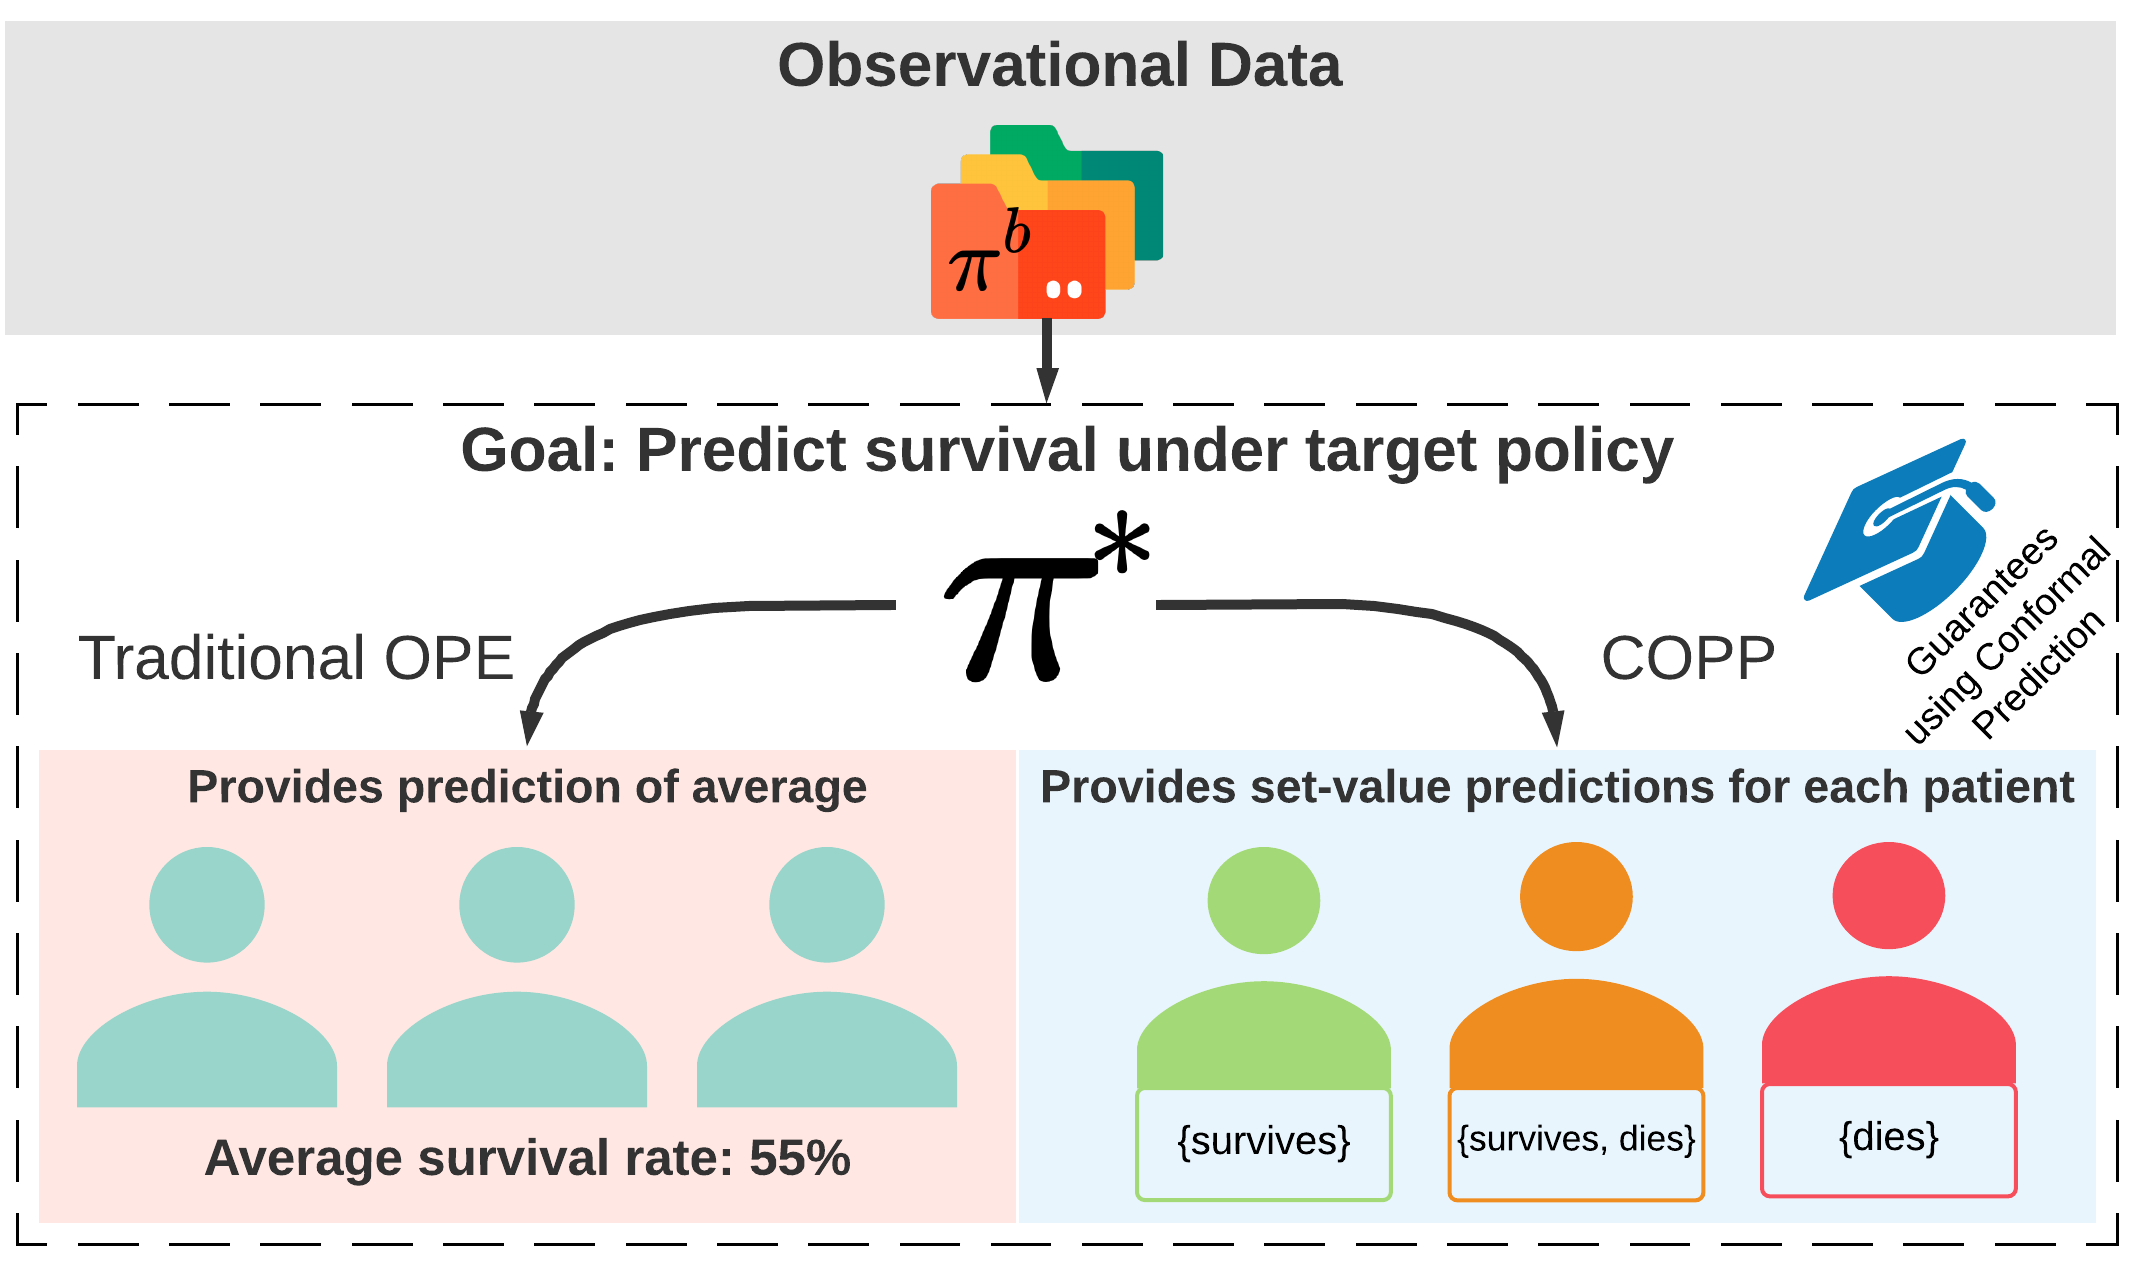
\includegraphics[width=0.5\columnwidth]{figures/copp/COPP5.png}
%     \caption{Illustration of Conformal Off-Policy Prediction compared to standard off-policy evaluation methods.}
%     \label{fig:copp}
% \end{figure}
Notable exceptions in the OPE literature are \cite{risk-assessment, chandak2021universal}. Instead of estimating bounds on the expected outcomes, \cite{risk-assessment, chandak2021universal} establish finite-sample bounds for a general class of metrics (e.g., Mean, CVaR, CDF) on the outcome. Their methods can be used to estimate quantiles of the outcomes under the target policy and are therefore robust to outliers. However, the resulting bounds do not depend on the covariates $X$ (not adaptive w.r.t. $X$). This can lead to overly conservative intervals, as we will show in our experiments and can become uninformative when the data are heteroscedastic (see Fig. \ref{fig:copp}b).

%  Instead of investigating the bounds on the expected outcomes, \cite{risk-assessment, chandak2021universal} propose an off-policy assessment in contextual bandits setting to construct bounds that enjoy finite-sample guarantees. In particular, the authors aim to construct estimators for the CDF of the return and hence are able determine quantities such as the median or the $95\%$ quantiles of the rewards, which as mentioned above, are crucial for robustness and uncertainty quantification. Note that the CDF estimators proposed by \cite{risk-assessment, chandak2021universal} do not depend on the specific $X$, and as a result the bounds obtained are not adaptive w.r.t. $X$. 

% Furthermore, while the distributional perspective without CDFs has been explored in the context of Reinforcement Learning \cite{distributional-rl}, to the best of our knowledge they do not provide any finite-sample guarantees.

% In this paper, we propose Conformal Off-Policy Prediction (COPP), a novel algorithm based on Conformal Prediction (CP) that produces predictive interval/sets for off-policy outcomes in contextual bandits (see Fig.\ref{fig:copp}a).
% To the best of our knowledge, this is the first method to obtain predictive intervals in the off-policy setting that enjoys both finite-sample theoretical guarantees and adaptivity w.r.t.\ the covariates $X$.
% % We achieve this by using conformal prediction (CP), a distribution-free uncertainty quantification method pioneered by \cite{vovk2005algorithmic}.
% %and can be used on top of any black-box model.
% Unlike previous work, which assumed a deterministic target and discrete action space, our approach is valid for stochastic target policies and continuous action spaces, which lifts the restriction of previous related work to deterministic targets and discrete actions.
% %, our approach can be applied to both deterministic and stochastic target policies, as well as discrete and continuous actions spaces.}

% In this paper, we propose Conformal Off-Policy Prediction (COPP), a novel algorithm for constructing predictive interval/sets for off-policy outcomes in contextual bandits (see Fig.\ref{fig:copp}a).
In this paper, we propose Conformal Off-Policy Prediction (COPP), a novel algorithm that uses Conformal Prediction (CP) \citep{vovk2005algorithmic} to construct predictive interval/sets for outcomes in contextual bandits (see Fig.\ref{fig:copp}a) using an observational dataset.
COPP enjoys both finite-sample theoretical guarantees and adaptivity w.r.t.\ the covariates $X$, and, to the best of our knowledge, is the first such method based on CP that can be applied to stochastic policies and continuous action spaces.
% To the best of our knowledge, COPP is the first such method that enjoys both finite-sample theoretical guarantees and adaptivity w.r.t.\ the covariates $X$.
% Unlike earlier work, our approach can be applied to stochastic policies and continuous action spaces.
% Unlike related work involving CP, our approach can be applied to both deterministic and stochastic target policies
% We achieve this via conformal prediction (CP), a distribution-free uncertainty quantification method pioneered by \cite{vovk2005algorithmic}.
%and can be used on top of any black-box model.

% % {\color{red} Our approach also applies to stochastic target policies which have not been considered by previous work on CP.}
% % Most importantly, CP produces predictive intervals that have finite-sample coverage guarantees, i.e. the interval will contain the ground truth outcome with a certain user pre-specified threshold $\alpha$.
% Our paper also makes the following additional contributions.
% (i)
% % Our approach is widely applicable: previous work involving CP has been limited to deterministic policies and discrete action spaces, while our method applies also for discrete and continuous.
% % Our approach is more widely applicable than previous work involving CP, and can be used for stochastic policies and continuous action spaces.
% % Our approach lifts restrictions present in related work involving CP, 
% % \R{Unlike related work involving CP, our approach can be applied to both deterministic and stochastic target policies, as well as discrete and continuous actions spaces.}
% \R{Our approach remains valid for stochastic target policies and continuous action spaces, which lifts the restriction of previous related work to deterministic targets and discrete actions.} %, our approach can be applied to both deterministic and stochastic target policies, as well as discrete and continuous actions spaces.}
% % \R{Unlike related work involving CP, our approach can be applied to both deterministic and stochastic target policies}
% % (ii) We provide theoretical guarantees for COPP, including finite-sample guarantees on marginal coverage and asymptotic guarantees on conditional coverage.
% (ii) We provide a theoretical analysis of COPP, including finite-sample guarantees on marginal coverage and asymptotic guarantees on conditional coverage.
% (iii) We show empirically that COPP outperforms standard methods in terms of coverage and predictive interval width when assessing new policies. 

% {\color{red} Our approach also applies to stochastic target policies which have not been considered by previous work on CP.}
% Most importantly, CP produces predictive intervals that have finite-sample coverage guarantees, i.e. the interval will contain the ground truth outcome with a certain user pre-specified threshold $\alpha$.
In summary, our contributions are: 
% (i) We adapt results from the CP literature to construct predictive intervals for the outcome $Y$ under a new policy which are adaptive w.r.t.\ $X$.
% (i) We construct valid predictive intervals for bandit outcomes that applies in more general settings (stochastic policies and continuous actions) than previous work.
(i) We propose an application of CP to construct predictive intervals for bandit outcomes that is more general (applies to stochastic policies and continuous actions) than previous work.
% Our approach is widely applicable: previous work involving CP has been limited to deterministic policies and discrete action spaces, while our method applies also for discrete and continuous.
% Our approach is more widely applicable than previous work involving CP, and can be used for stochastic policies and continuous action spaces.
% Our approach lifts restrictions present in related work involving CP, 
% \R{Unlike related work involving CP, our approach can be applied to both deterministic and stochastic target policies, as well as discrete and continuous actions spaces.}
% \R{Our approach avoids various restrictions of earlier work, being valid for stochastic target policies and continuous action spaces.} %, our approach can be applied to both deterministic and stochastic target policies, as well as discrete and continuous actions spaces.}
% \R{Unlike related work involving CP, our approach can be applied to both deterministic and stochastic target policies}
(ii) We provide theoretical guarantees for COPP, including finite-sample guarantees on marginal coverage and asymptotic guarantees on conditional coverage.
(iii) We show empirically that COPP outperforms standard methods in terms of coverage and predictive interval width when assessing new policies. 

\subsection{Problem Setup}\label{sec:problem_setup}

\begin{comment}
% \begin{wrapfigure}{r}{0.22\textwidth}
\begin{figure}
    \centering
    \includegraphics[width=0.15\textwidth]{diagram1.pdf}
    \caption{Causal graph of our problem setup. The action $A$ is shaded to illustrate that we are ``integrating out'' the effect of the actions through the policy when predicting $Y$ from $X$.}
    \label{fig:OPE_conformal}
\end{figure}
% \end{wrapfigure}
\end{comment}
Let $\mathcal{X}$ be the covariate space (e.g., user  data), $\mathcal{A}$ the action space (e.g., recommended items) and $\mathcal{Y}$ the outcome space (e.g., relevance to the user).
We allow both $\mathcal{A}$ and $\mathcal{Y}$ to be either discrete or continuous.
In our setting, we are given logged observational data $\mathcal{D}_{obs}=\{x_i, a_i, y_i \}_{i=1}^{n_{obs}}$ where actions are sampled from a behavioural policy $\pi^{b}$, i.e. $A \mid x \sim \pi^{b}(\cdot\mid x)$ and $Y \mid x,a \sim P(\cdot \mid x, a)$. We assume that we do not suffer from unmeasured confounding. At test time, we are given a state $x^{test}$ and a new policy $\pi^*$. While $\pi^{b}$ may be unknown, we assume the target policy $\pi^*$ to be known.
% \begin{comment}
% \begin{align*}
%     \text{Standard OPE} \qquad & \mathbb{E}_{(X, Y) \sim P^{\pi^*}_{X,Y}}[Y] \\
%     \text{Huang} \qquad & \mathbb{E}_{(X, Y) \sim P^{{\pi^*}}_{X,Y}} [\varphi(Y)], \varphi \in \Phi \\
%     \text{Us} \qquad &  \hat{C} \text{ s.t. } 1- \alpha \hspace{-0.05cm}\leq  \tarprob(Y \in \hat{C}(X)) \hspace{-0.05cm}\leq 1- \alpha + o_{n_{obs}}(1)
% \end{align*}
% \end{comment}
% \begin{comment}
% % Properties of interest: 1. adaptivity w.r.t x 2. capturing of the variability in outcomes 3. finite sample guarantees. 
% In this paper we aim to construct intervals $\hat{C}(x)$ on the outcome $Y$ which are (i) dependent on $x$, (ii) capture the variability in outcomes $Y$ and (iii) provide finite sample guarantees. Current explored methodologies lack at least one of these properties (see Table [] in section). 
% In particular, property (ii) can be achieved if $\hat{C}(x)$ captures the true outcome $Y$ with any pre-specified probability $1-\alpha$. One way to express this formally is as follows:
% \begin{align}
%      \hspace{-0.24cm}1- \alpha \hspace{-0.05cm}\leq  \tarprob(Y \in \hat{C}(X)) \hspace{-0.05cm}\leq 1- \alpha + o_{n_{obs}}(1) \label{guarantee}
% \end{align}
% where $n_{obs}$ is the size of available observational data and $P^{\pi^*}_{X,Y}$ is the joint distribution of $(X,Y)$ under target policy $\pi^*$. The probability is taken over the joint distribution of $(X, Y)$, meaning that the interval holds in the marginal sense in $X$ (marginal coverage) and not for a given $X=x$ (conditional coverage). In Section \ref{sec:cond_cov}, we provide additional regularity conditions under which not only marginal but also conditional coverage holds. Moreover, given that we are interested in the outcomes under $\pi^*$, the intervals $\hat{C}(x)$ are not conditioned on a specific $a$, but rather on $\pi^*$. 
% In this paper, we construct $\hat{C}(x)$ which satisfies \eqref{guarantee} along with the properties (i)-(iii), using the CP framework, which we will introduce in the following section. 
% % Our proposed methodology uses CP to construct $\hat{C}(x)$ and provides finite-sample coverage guarantees on the outcomes $Y$ given a current state $X$ and a target policy $\pi^* (a\mid x)$, hence allowing us to be confident in terms of the outcomes, when deploying a new policy.
% % \textbf{Explanation of the objective: } 
% % The :
% % Standard OPE & \mathbb{E}_{(X, Y) \sim P^{\pi^*}_{X,Y}}[Y] & (1) x (2) x (3) \tick
% % Huang et al & \mathbb{E}_{(X, Y) \sim P^{\pi^*}_{X,Y}}[\phi(Y]) & (1) \tick 2(x) (3) \tick
% % In this setting the quantities of interests in the current literature are:
% % \begin{align*}
% %     \text{Standard OPE} \qquad & \mathbb{E}_{(X, Y) \sim P^{\pi^*}_{X,Y}}[Y] \\
% %     \text{Huang} \qquad & \mathbb{E}_{(X, Y) \sim P^{{\pi^*}}_{X,Y}} [\varphi(Y)], \varphi \in \Phi
% % \end{align*}
% % However, none of these objectives take into account take into account both the finite sample guarantees and the adaptivity w.r.t. $x$. Hence we propose to construct predictive intervals on the outcomes which are adaptive w.r.t. $x$, and provide finite sample guarantees
% In standard OPE literature the main objective is to estimate $\mathbbm{E}[sth]$
% \end{comment}
% \textbf{Our goal} is to obtain predictive intervals/sets, $\hat{C}(x^{test})$, for a given $\alpha \in (0,1)$, which satisfy:
% \begin{align}
% \text{$P_{Y(a)}(y \mid X = x)$ for each $a$} \\
% \text{$C_a$ such that $\mathbb{P}(Y(a) \in C_a(X) \mid X = x) \geq 1 - \alpha$, for each $a$} \\
% \text{$C_a$ such that $\mathbb{P}(Y(a) \in C(X)) \geq 1 - \alpha$ for each $a$}
% \end{align}
% \begin{align}
%      \hspace{-0.24cm}1- \alpha \hspace{-0.05cm}\leq  \tarprob(Y \in \hat{C}(X)) \hspace{-0.05cm}\leq 1- \alpha + o_{n_{obs}}(1) \label{guarantee}
% \end{align}
% where $n_{obs}$ is the size of available observational data and $P^{\pi^*}_{X,Y}$ is the joint distribution of $(X,Y)$ under target policy $\pi^*$. Note that the probability is taken over the joint distribution of $(X, Y)$, meaning that the interval holds in the marginal sense in $X$ (marginal coverage) and not for a given $X=x$ (conditional coverage).  In Section \ref{sec:cond_cov}, we provide additional regularity conditions under which not only marginal but also conditional coverage holds.
% % The challenges in this case are to account for the shift in policy and obtain guarantees on the predictive interval $\hat{C}(X)$.
% To this end, we will use the CP framework to construct predictive intervals in order to assess a new policy. Our proposed methodology provides theoretical coverage guarantees on the outcome $Y$ given a current state $X$ and a target policy $\pi^* (a\mid x)$, hence allowing us to be confident in terms of the outcomes, when deploying a new policy.
% Huang et al.\ obtain a method for obtaining a richer evaluation of a given policy.
% Specifically, they estimate the $\varphi(p^{\pi^\ast}_{X,Y})$ for a more general class of functions $\varphi$ than just the expectation operator.
% While this allows for a much richer understanding of $\pi^\ast$, its expressiveness is still in some respects limited, as is clear from the fact that it does not depend on $X$, but only on $P_{X,Y}^{\pi^\ast}$.
% 
% The guarantees they get are usually only asymptotic, meaning that they approximate this quantity with 

% Existing methods focus on evaluating $\mathbb{E}_{(X, Y)\sim P^{\pi^*}_{X,Y}}[Y]$.
% This is useful for comparing two policies directly because it is just a single number, but does not provide a rich understanding of the behaviour of the policy on a per item basis.

% In this work, we present a method that avoids some of these shortcomings.
% Specifically, we construct a set-valued function $\hat{C}(x)$ that takes as input a covariate and outputs a \emph{subset} of $\mathcal{Y}$ rather than just a single point.
% This subset is guaranteed to contain the true value of $Y$ with a certain probability.
% Specifically, we obtain the guarantee:
% \[
% \tarprob(Y \in \hat{C}(X)) \geq 1 - \alpha.
% \]
% Moreover, we will show this guarantee holds for our method regardless of any distributional assumptions on $X$ and $Y$, and regardless of the size of the data we have available to us.

We consider the task of rigorously quantifying the performance of $\pi^*$ without any distributional assumptions on $X$ or $Y$. Many existing approaches estimate $\mathbb{E}_{\pi^*}[Y]$, which is useful for comparing two policies directly as they return a single number. However, the expectation does not convey fine-grained information about how the policy performs for a specific value of $X$, nor does it account for the uncertainty in the outcome $Y$.

Here, we aim to construct intervals/sets on the outcome $Y$ which are (i) adaptive w.r.t. $X$, (ii) capture the variability in the outcome $Y$ and (iii) provide finite-sample guarantees. Current methods lack at least one of these properties (see Sec. \ref{sec:related_work}). One way to achieve these properties is to construct a set-valued function of $x$, $\hat{C}(x)$ which outputs a \emph{subset} of $\mathcal{Y}$. Given any finite dataset $\mathcal{D}_{obs}$, this subset is guaranteed to contain the true value of $Y$ with any pre-specified probability, i.e.
\begin{align}
     \hspace{-0.24cm}1- \alpha \hspace{-0.05cm}\leq  \tarprob(Y \in \hat{C}(X)) \hspace{-0.05cm}\leq 1- \alpha + o_{n_{obs}}(1) \label{guarantee}
\end{align}
where $n_{obs}$ is the size of available observational data and $P^{\pi^*}_{X,Y}$ is the joint distribution of $(X,Y)$ under target policy $\pi^*$. In practice, $\hat{C}(x)$ can be used as a diagnostic tool downstream for a granular assessment of likely outcomes under a target policy. The probability in (\ref{guarantee}) is taken over the joint distribution of $(X, Y)$, meaning that \eqref{guarantee} holds marginally in $X$ (marginal coverage) and not for a given $X=x$ (conditional coverage). In Sec. \ref{sec:cond_cov}, we provide additional regularity conditions under which not only marginal but also conditional coverage holds. Next, we introduce the Conformal Prediction framework, which allows us to construct intervals $\hat{C}(x)$ that satisfy \eqref{guarantee} along with properties (i)-(iii). 

\section{Background}
Conformal prediction \citep{vovk2005algorithmic, shafer2008tutorial} is a methodology that was originally used to compute distribution-free prediction sets for regression and classification tasks. Before introducing COPP, which applies CP to contextual bandits, we first illustrate how CP can be used in standard regression.

% In this section, we illustrate the application of CP in a standard regression setting. 

% For illustrative purposes, we will consider the former in this section.
% we have considered a standard regression problem in this section.

\subsection{Standard Conformal Prediction} 
% Conformal prediction \cite{shafer2008tutorial, vovk2005algorithmic} is a methodology used to compute distribution-free prediction intervals. It was classically designed for regression and classification problems.       

% We split the available observations $\mathcal{D}_{obs}=\{X_i,Y_i \}_{i=1}^{n_{obs}}$ into a \emph{calibration} set $\mathcal{D}_{cal} = \{X_i, Y_i\}_{i\in \mathcal{I}_{cal}}$, where $\mathcal{I}_{cal}=\{1,\dots,n\}$, and a \emph{training} set $\mathcal{D}_{tr} = \{X_i^0, Y_i^0\}_{i\in \mathcal{I}_{tr}}$ where $\mathcal{I}_{tr}=\{1,\dots,N\}$.

% $\mathcal{D}_{tr} =  \mathcal{D}_{obs} \setminus \mathcal{D}_{cal}$ (of size $N$) onto which a regression model $\hat{f}$ is trained. The data in the calibration set are assumed to be i.i.d. from an arbitrary distribution $P_{X,Y}$. 

Consider the problem of regressing $\mbox{Y} \in \mathcal{Y}$ against $X\in \mathcal{X}$.
Let $\hat{f}$ be a model trained on the \emph{training} data $\mathcal{D}_{tr} = \{X_i^0, Y_i^0\}_{i=1}^m \overset{\textup{i.i.d.}}{\sim} P_{X,Y}$ and let the \emph{calibration} data $\mathcal{D}_{cal} = \{X_i, Y_i\}_{i=1}^n \overset{\textup{i.i.d.}}{\sim} P_{X,Y}$ be independent of $\mathcal{D}_{tr}$. Given a desired coverage rate $1-\alpha \in (0,1)$, we construct a band $\hat{C}_n:\mathcal{X}\rightarrow \{\text{subsets of }\mathcal{Y}\}$, based on the calibration data such that, for a new i.i.d. test data $(X,Y) \sim P_{X,Y}$,
\begin{align}
    1-\alpha \leq \mathbb{P}_{(X,Y)\sim P_{X,Y}}(Y\in \hat{C}_n(X)) \leq 1-\alpha + \frac{1}{n+1}, \label{cp_guarantee}
\end{align}
where the probability is taken over $X,Y$ and $\mathcal{D}_{cal} = \{X_i, Y_i\}_{i=1}^n$ and is conditional upon $\mathcal{D}_{tr}$.

% \yw{so there's $X_i$ in  train set and $X_i$ in calibration set? Note both index sets start at 1, so not disjoint. but we have i in $I_cal$ and $I_tr$ one is from 1 to N and the other from N+1 to N+n. Read your paragraph above. I think you've updated your definition of $I_{cal}$ to be disjoint. Note that there is inconsistency with indexing of $X_{n+1}$, $Y_{n+1}$ now. oh i see you are right let me fix the notation now should be 1 to n and then n+1 to n+N}

In order to obtain $\hat{C}_n$ satisfying \eqref{cp_guarantee}, we introduce a non-conformity score function $V_i = s(X_i, Y_i)$, e.g., $(\hat{f}(X_i) - Y_i)^2$. We assume here $\{V_i\}_{i=1}^n$ have no ties almost surely. Intuitively, the non-conformity score $V_i$ uses the outputs of the predictive model $\hat{f}$ on the calibration data, to measure how far off these predictions are from the ground truth response. Higher scores correspond to worse fit between $x$ and $y$ according to $\hat{f}$. We define the empirical distribution of the scores $\{V_i\}_{i=1}^n \cup \{\infty\}$
\begin{align}\label{eq:std_emp_score}
 \hat{F}_{n} \coloneqq \frac{1}{n+1} \sum_{i=1}^n \delta_{V_i} + \frac{1}{n+1}\delta_{\infty}  
\end{align}
with which we can subsequently construct the conformal interval $\hat{C}_n$ that satisfies \eqref{cp_guarantee} as follows:
\begin{align}
    \hat{C}_n(x) \coloneqq \{y: s(x,y) \leq \eta\} \label{eq:interval}
\end{align}
where $\eta$ is an empirical quantile of $\{V_i\}_{i=1}^n$, i.e. $\eta = \text{Quantile}_{1-\alpha}(\hat{F}_{n})$ is the $1-\alpha$ quantile.

Intuitively, for roughly $100\cdot(1-\alpha) \%$ of the calibration data, the score values will be below $\eta$. Therefore, if the new datapoint $(X, Y)$ and $\mathcal{D}_{cal}$ are i.i.d., the probability $\p(s(X,Y) \leq \eta)$ (which is equal to $\p(Y \in \hat{C}_n(X))$ by \eqref{eq:interval}) will be roughly $1-\alpha$. Exchangeability of the data is crucial for the above to hold. In the next section we will explain how \cite{tibshirani2020conformal} relax the exchangeability assumption.
% Hence, due to the i.i.d. assumption of the calibration and test data, it would not make sense to include $y$'s that induce a score higher than $\eta$ when targeting $100\cdot(1-\alpha) \%$ coverage guarantees. It should also be noted that exchangeability\footnote[1]{Exchangeability is sufficient and we do not need i.i.d.} of the data is crucial for the above to hold. In the next section we will explain how \cite{tibshirani2020conformal} relax this assumption.

% In essence, $\hat{C}_n(x)$ will only contain $y$'s for which the score is ``not too big'' i.e. is less than the $\lceil(n+1)(1-\alpha)\rceil/n$ quantile of the scores in the calibration data. Note that due to exchangeability and as long as the $s(x,y)$ is below the quantile, we can guarantee that the resulting interval will contain the ground truth with probability at least $1-\alpha$. 
% The original formulation of CP relies only on exchangeability of the calibration and test data. A brief summary of CP steps is given in algorithm \ref{cp}. Note that here we use the notation Quantile$(\beta; F)$ to denote the level $\beta$ quantile of a distribution F, i.e. for $Z\sim F$,
% \[
%     \text{Quantile}(\beta; F) = \inf \{z : \mathbb{P}(Z\leq z) \geq \beta \}
% \]

% It can be shown that the predictive intervals $\hat{C}_n(x)$ obtained through algorithm \ref{cp} satisfy the following guarantee
% \[
% 1-\alpha \leq \mathbb{P}(Y_{n+1}\in \hat{C}_n(X_{n+1})) \leq 1-\alpha + \frac{1}{n+1}
% \]
% \begin{algorithm}
% \SetAlgoLined
% \textbf{Inputs:} Trained model $\hat{f}$; calibration data $\{X_i, Y_i\}_{i=1}^n$; New data point $x$, confidence level $\alpha$\\
% \textbf{Output:} Confidence set $\hat{C}_n(x)$ which satisfies (\ref{cp_guarantee})\\
% Define the score function $s(X,Y)\in\mathbb{R}$ (larger scores encode worse fit between $X$ and $Y$).\;
% \For{i = 1, \dots, n}{
% $V_i \coloneqq s(X_i, Y_i)$\;
% }
% Define the empirical distribution $\hat{F}_{n} \coloneqq \frac{1}{n+1} \sum_{i=1}^n \delta_{V_i} + \frac{1}{n+1}\delta_{\infty}$\;
% For a new data point $x$, $\hat{C}_n(x) \coloneqq \{y: s(x,y) \leq \text{Quantile}(\lceil(n+1)(1-\alpha)\rceil/n, \hat{F}_{n})\}$\;
% \textbf{Return} $\hat{C}_n(x)$
%   \caption{Conformal prediction algorithm}
%   \label{cp}
% \end{algorithm}

\subsection{Conformal Prediction under covariate shift}\label{CP_cov_shift}
\cite{tibshirani2020conformal} extend the CP framework beyond the setting of exchangeable data, by constructing valid intervals even when the calibration data and test data are not drawn from the same distribution. The authors focus on the \textit{covariate shift} scenario i.e. the distribution of the covariates changes at test time:
\begin{align}
    &(X_i, Y_i) \overset{\textup{i.i.d}}{\sim} P_{X,Y} = P_X \times P_{Y\mid X}, \quad i = 1, \dots, n \nonumber \\
    &(X, Y) \sim \tilde{P}_{X,Y} = \tilde{P}_{X} \times P_{Y\mid X},~\text{independently}\nonumber
\end{align}

% \begin{center}
% \begin{tabular}{l}
%             \small $(X_i, Y_i) \overset{\textup{i.i.d}}{\sim} P_{X,Y} = P_X \times P_{Y\mid X}, \quad i = 1, \dots, n$\\ 
%             \small $(X, Y) \sim \tilde{P}_{X,Y} = \tilde{P}_{X} \times P_{Y\mid X},~\text{independently}$
% \end{tabular}
% \end{center}
where the ratio $w(x)\coloneqq\mathrm{d}\tilde{P}_{X}/\mathrm{d}P_{X}(x)$ is known.
The key realization in \cite{tibshirani2020conformal} is that the requirement of \textit{exchangeability} in CP can be relaxed to a more general property, namely \textit{weighted exchangeability} (see Def. \ref{def:weighted_exch}). 
% The key realization is by firstly noting that the calibration and test data are \textit{weighted exchangeable}, which is more general property than \textit{exchangeability}.
% Secondly, if we know the ratio of test to calibration covariate likelihoods, we can define $w(x) = d\tilde{P}_{X}(x)/dP_{X}(x)$. 
They propose a weighted version of conformal prediction, which shifts the empirical distribution of non-conformity scores, $\hat{F}_{n}$, at a point $x$, using weights $w(x)$. This adjusts $\hat{F}_{n}$ for the covariate shift, before picking the quantile $\eta$: $$\hat{F}_{n}^{x} \coloneqq  \sum_{i=1}^n p_i^w(x) \delta_{V_i} + p_{n+1}^w(x)\delta_{\infty}\quad \textup{ where,}$$ 
\begin{align*}
    p_i^{w}(x) = \frac{w(X_i)}{\sum_{j=1}^n w(X_j) + w(x)}, \quad p_{n+1}^{w}(x) = \frac{w(x)}{\sum_{j=1}^n w(X_j) + w(x)}.
\end{align*}

% \begin{align}
%     \hat{F}_{n}^{x} \coloneqq  \sum_{i=1}^n p_i^w(x) \delta_{V_i} + p_{n+1}^w(x)\delta_{\infty}, \nonumber
% \end{align}



% $p_i^w(x) \propto w(X_i)$ for $i \in \{1,...,N\}$, $p^w_{n+1}(x)\propto w(x)$ with $\sum_{i=1}^{n+1} p^w_i(x)=1$. \yw{much notational problem here. what's $x$? I can't parse "$p^w_i(x) \propto w(X_i)$". Is it $n$ or $N$?}  

In standard CP (without covariate shift), the weight function satisfies $w(x)=1$ for all $x$, and we recover \eqref{eq:std_emp_score}. Next, we construct the conformal prediction intervals $\hat{C}_n$ as in standard CP using \eqref{eq:interval} where $\eta$ now depends on $x$ due to $p^w_i(x)$. The resulting intervals, $\hat{C}_n$, satisfy: 
% \yw{not sure I understand this point re dependence on $x$. what's $x$ actually?}
% \begin{align*}
%     1-\alpha \leq \mathbb{P}_{(X,Y)\sim \tilde{P}_{X, Y}}(Y\in \hat{C}_n(X)) \leq 1-\alpha + cn^{1/r-1}    
% \end{align*}
\begin{align*}
     \mathbb{P}_{(X,Y)\sim \tilde{P}_{X, Y}}(Y\in \hat{C}_n(X)) \geq 1-\alpha    
\end{align*}
As mentioned previously in Sec. \ref{sec:problem_setup}, the above demonstrates marginal coverage guarantees over test point $X$ \faaiz{and calibration dataset $\mathcal{D}_{cal}$, not conditional on a given $X=x$ or a fixed $\mathcal{D}_{cal}$}.  We will discuss this nuance later on in Sec. \ref{sec:cond_cov}. In addition, previous work by \citeauthor{vovk2012} shows that conditioned on a single calibration dataset, standard CP can achieve coverage that is `close' to the required coverage with high probability. However, this has not been extended to the case where the distribution shifts. This is out of the scope of this paper and an interesting future direction. 


\begin{algorithm}[!htp]
\SetAlgoLined
\textbf{Inputs:} Observational data $\mathcal{D}_{obs}=\{X_i, A_i, Y_i\}_{i=1}^{n_{obs}}$, conf. level $\alpha$, a score function $s(x,y)\in\mathbb{R}$, new data point $x^{test}$, target policy $\pi^*$ \;
\textbf{Output:} Predictive interval $\hat{C}_n(x^{test})$\;
Split $\mathcal{D}_{obs}$ into training data ($\mathcal{D}_{tr}$) and calibration data ($\mathcal{D}_{cal}$) of sizes $m$ and $n$ respectively\;
Use $\mathcal{D}_{tr}$ to estimate weights $\hat{w}(\cdot, \cdot)$ using \eqref{weight-est}\;
Compute $V_i \coloneqq s(X_i, Y_i)$ for $(X_i, A_i, Y_i) \in \mathcal{D}_{cal}$\;
Let $\hat{F}_{n}^{x, y}$ be the weighted distribution of scores 
$\hat{F}_{n}^{x, y} \coloneqq  \sum_{i=1}^n p_i^{\hat{w}}(x, y) \delta_{V_i} + p_{n+1}^{\hat{w}}(x, y)\delta_{\infty}$\\
where $p_i^{\hat{w}}(x, y) = \frac{\hat{w}(X_i, Y_i)}{\sum_{j=1}^n \hat{w}(X_j, Y_j) + \hat{w}(x, y)}$ and $p_{n+1}^{\hat{w}}(x, y) = \frac{\hat{w}(x, y)}{\sum_{j=1}^n \hat{w}(X_j, Y_j) + \hat{w}(x, y)}$\;
% \textcolor{red}{Define the empirical distribution $\hat{F}_{n} \coloneqq  \sum_{i=1}^n p_i^w(x) \delta_{V_i} + p_{n+1}^w(x)\delta_{\infty}$}\;
% \textcolor{red}{where $p_i^w(x) = \frac{w(X_i)}{\sum_{j=1}^n w(X_j) + w(x)}$ and $p_{n+1}^w(x) = \frac{w(x)}{\sum_{j=1}^n w(X_j) + w(x)}$}\;


% Define the empirical distribution of the scores as:
% $$
% \hat{\mathcal{F}}_{n}^{x, y} \coloneqq 
% \begin{cases}
% \hat{F}_{n} &\text{for standard CP }   \eqref{eq:std_emp_score}\\ 
% \hat{F}_{n}^{x}  &\text{for cov. shifted CP }  \eqref{eq:cov_shift_emp_score}\\
% \hat{F}_{n}^{x, y}  &\text{for policy shifted CP }  \eqref{score-dist-pshift}\\
% \end{cases}
% $$
For $x^{test}$ construct:
% $$\hat{C}_n(x^{test}) \coloneqq \{y: s(x^{test},y) \leq \text{Quantile}(1-\alpha, \hat{F}_{n})\}$$
% $$\hat{C}_n(x^{test}) \coloneqq \{y: s(x^{test},y) \leq \text{Quantile}(1-\alpha, \hat{F}_{n}^{x})\}$$
$
    \hat{C}_n(x^{test})\hspace{-0.1cm} \coloneqq \{y: s(x^{test},y) \leq \text{Quantile}_{1-\alpha}(\hat{F}_{n}^{x^{test}, y})\} \nonumber
$

\textbf{Return} $\hat{C}_n(x^{test})$
  \caption{Conformal Off-Policy Prediction (COPP)}
  \label{cp_covariate_shift}
\end{algorithm}

Thus \cite{tibshirani2020conformal} show that the CP algorithm can be extended to the setting of covariate shift with the resulting predictive intervals satisfying the coverage guarantees when the weights are known. The extension of these results to approximate weights was proposed in  \cite{lei2020conformal} and is generalized to our setting in Sec. \ref{sec:theory}. 
\section{Conformal Off-Policy Prediction (COPP)}
% \subsection{Conformal Prediction with policy shift}
In the contextual bandits introduced in Sec. \ref{sec:problem_setup}, we assume that the observational data $\mathcal{D}_{obs} = \{x_i, a_i, y_i\}_{i=1}^{n_{obs}}$ is generated from a behavioural policy $\pi^b$. At inference time we are given a new target policy $\pi^*$ and want to provide intervals on the outcomes $Y$ for covariates $X$ that satisfy \eqref{guarantee}.

% Before diving deeper into our proposed method, we would like to highlight certain aspects of the problem. Firstly, the key difference between covariate shifted CP and our problem setting is the following: For covariate shifted CP, we are provided with an unseen data point $x^{test}$ for which we want to find a predictive interval $\hat{C}(x^{test})$. However, in our setting we are given $x^{test}$ \textbf{and} a target policy $\pi^*$, i.e. a function and hence needs to be taken care of appropriately. Secondly, contrary to {tibshirani2020conformal}, who look into a shift in $P_X$, we are instead interested in the shift in policies, which, as we show in this section, corresponds to a conditional shift in $P_{Y|X}$.
The key insight of our approach is to consider the following joint distribution of $(X,Y)$:
% \begin{align*}
%     P^{\pi^{b}}(x, y) \hspace{-0.1cm} &= \hspace{-0.1cm} P(x) \int P(y| x, a) \textcolor{red}{\pi^{b}(a|x)} \mathrm{d}a  =P(x) \textcolor{red}{P^{\pi^{b}}(y|x)} \\
%     P^{\pi^*}(x, y)\hspace{-0.1cm} &= \hspace{-0.1cm} P(x)\int P(y| x, a) \textcolor{red}{\pi^*(a|x)}  \mathrm{d}a = P(x)\textcolor{red}{P^{\pi^*}(y|x)}
% \end{align*}
% \begin{center}
% \begin{tabular}{c}
%             \small $P^{\pi^{b}}(x, y) \hspace{-0.1cm} = \hspace{-0.1cm} P(x) \int P(y| x, a) \textcolor{red}{\pi^{b}(a|x)} \mathrm{d}a  =P(x) \textcolor{red}{P^{\pi^{b}}(y|x)}$\\ 
%             \small $P^{\pi^*}(x, y)\hspace{-0.1cm} = \hspace{-0.1cm} P(x)\int P(y| x, a) \textcolor{red}{\pi^*(a|x)}  \mathrm{d}a = P(x)\textcolor{red}{P^{\pi^*}(y|x)}$
% \end{tabular}
% \end{center}
\begin{align*}
    P^{\pi^{b}}(x, y)=& P(x) \int P(y| x, a) \textcolor{red}{\pi^{b}(a|x)} \mathrm{d}a  =P(x) \textcolor{red}{P^{\pi^{b}}(y|x)} \\
    P^{\pi^*}(x, y) =& P(x)\int P(y| x, a) \textcolor{red}{\pi^*(a|x)}  \mathrm{d}a = P(x)\textcolor{red}{P^{\pi^*}(y|x)}
\end{align*}

Therefore, the change of policies from $\pi^b$ to $\pi^*$ causes a shift in the joint distributions of $(X, Y)$ from $P^{\pi^{b}}_{X, Y}$ to $P^{\pi^*}_{X, Y}$. More precisely, a shift in the conditional distribution of $Y|X$. As a result, our problem boils down to using CP in the setting where the conditional distribution $P^{\pi^{b}}_{Y\mid X}$ changes to $P^{\pi^{*}}_{Y \mid X}$ due to the different policies, while the covariate distribution $P_X$ remains the same. 
% =\mathrm{d}P^{\pi^{*}}_{X,Y}/\mathrm{d}P^{\pi^{b}}_{X,Y}(x,y)

Hence our problem is not concerned about covariate shift as addressed in \cite{tibshirani2020conformal}, but instead uses the idea of \textit{weighted exchangeability} to extend CP to the setting of policy shift. To account for this distributional mismatch, our method shifts the empirical distribution of non-conformity scores at a point $(x, y)$ using the weights $w(x,y) = \mathrm{d}P^{\pi^{*}}_{X,Y}/\mathrm{d}P^{\pi^{b}}_{X,Y}(x,y) = \mathrm{d}P^{\pi^{*}}_{Y|X}/\mathrm{d}P^{\pi^{b}}_{Y|X}(x,y)$:
\begin{align}
   \textstyle  \hat{F}_{n}^{x, y} &\coloneqq \sum_{i=1}^n p_i^w(x, y)\delta_{V_i} + p_{n+1}^w(x,y)\delta_\infty, \label{score-dist-pshift}
\end{align}
\begin{align*}
p_i^{w}(x, y)= \frac{w(X_i, Y_i)}{\sum_{j=1}^n w(X_j, Y_j) + w(x, y)}, \quad
p_{n+1}^{w}(x, y) = \frac{w(x, y)}{\sum_{j=1}^n w(X_j, Y_j) + w(x, y)}. 
\end{align*}


% \begin{center}
% \end{center}
% Our work builds upon the idea of conformal prediction under covariate shift proposed by \cite{tibshirani2020conformal}  exploited to quantify uncertainty in individual treatment effects by \cite{lei2020conformal}. 
% In our problem, the main challenge arises from the fact that there is a distributional mismatch between calibration ($\mathcal{D}_{cal}\subset \mathcal{D}_{obs}$) and test data. The observational data is generated using a behaviour policy $\pi^b$, whereas the predictive intervals that we seek must hold under data generated from a different target policy $\pi^*$ (for which we have no data). This shift in distribution means that standard CP can no longer be used. However, as we show next,
% This observation thus allows us to assess unseen policies $\pi^*$ based on observational data collected using $\pi^b$. 
% We note that, similar to \cite{tibshirani2020conformal}, we can use the idea of \textit{weighted exchangeability} to extend CP to our setting. 
% the calibration and test data in our setting are weighted exchangeable, with weights $w(x,y) =\mathrm{d}P^{\pi^{*}}_{X,Y}/\mathrm{d}P^{\pi^{b}}_{X,Y}(x,y)= \mathrm{d}P^{\pi^{*}}_{Y|X}/\mathrm{d}P^{\pi^{b}}_{Y|X}(x,y)$. Hence, we can extend the weighted version of CP to account for policy shift in the empirical distribution of non-conformity scores:
% $p_i^w(x, y) \propto w(X_i, Y_i)$ for $i \in \{1,...,n\}$, $p^w_{n+1}(x, y)\propto w(x, y)$ with $\sum_{i=1}^{n+1} p^w_i(x, y)=1$.
% where $p_{i}^w(x, y) \coloneqq \frac{w(X_i, Y_i)}{\sum_{i=1}^n w(X_i, Y_i) + w(x,y)}$, $p_{n+1}^w(x, y) \hspace{-0.1cm} \coloneqq \hspace{-0.1cm} \frac{w(x,y)}{\sum_{i=1}^n w(X_i, Y_i) + w(x,y)}$. 
The intervals are then constructed as below which we call Conformal Off-Policy Prediction (Alg. \ref{cp_covariate_shift}).
% As before, the predictive intervals can be constructed using
\begin{align}
    \hat{C}_n(x^{test}) \coloneqq \{y: s(x^{test},y) \leq \eta(x^{test}, y)\} \hspace{0.2cm} \textup{where, }  \eta(x, y) \coloneqq \text{Quantile}_{1-\alpha}( \hat{F}_{n}^{x, y}). \label{cp-sets}
\end{align}
% We call this Conformal Off-Policy Prediction (Alg. \ref{cp_covariate_shift}).

\paragraph{Remark}
    The weights $w(x, y)$ in \eqref{score-dist-pshift} depend on $x$ and $y$, as opposed to only $x$. In particular, finding the set of $y$'s satisfying \eqref{cp-sets} becomes more complicated than for the standard covariate shifted CP which only requires a single computation of $\eta(x)$ for a given $x$ as shown in \eqref{eq:interval}. In our case however, we have to create a $k$ sized grid of potential values of $y$ for every $x$ to find $\hat{C}_n(x)$. This operation is embarrassingly parallel and hence does not add much computational overhead compared to the standard CP, especially because CP mainly focuses on scalar predictions.


\subsection{Estimation of weights $w(x, y)$}\label{sec:weights}
So far we have been assuming that we know the weights $w(x, y)$ exactly. However, in most real-world settings, this will not be the case. Therefore, we must resort to estimating $w(x, y)$ using observational data. In order to do so, we first split the observational data into training ($\mathcal{D}_{tr}$) and calibration ($\mathcal{D}_{cal}$) data. Next, using $\mathcal{D}_{tr}$, we estimate $\hat{\pi}^b(a\mid x) \approx \pi^b(a \mid x)$ and $\hat{P}(y \mid x, a) \approx P(y \mid x, a)$ (which is independent of the policy). We then compute a Monte Carlo estimate of weights using the following:
% \begin{align}\label{CP_new_weights}
%     w(x, y) = \frac{\int P(y|x, a) \textcolor{red}{\pi^*(a|x)} da}{\int P(y| x, a) \textcolor{red}{\pi^b(a|x)} da}
% \end{align} 
% which can subsequently be estimated using the monte carlo estimator:
\begin{align}
    \hat{w}(x, y) &= \frac{\tfrac{1}{h}\sum_{k=1}^{h} \hat{P}(y|x, A^*_k)}{\tfrac{1}{h} \sum_{k=1}^{h} \hat{P}(y|x, A_k)} \approx \frac{\int P(y|x, a) \textcolor{red}{\pi^*(a|x)} \mathrm{d}a}{\int P(y| x, a) \textcolor{red}{\pi^b(a|x)} \mathrm{d}a},  \label{weight-est}
\end{align}
where $A_k\sim \hat{\pi}^b(\cdot \mid x),~ A_k^* \sim  \pi^*(\cdot \mid x)$ and $h$ is the number of Monte Carlo samples.

\begin{importantresultwithtitle}[title=Why not construct intervals using \text{$\hat{P}(y|x, a)$} directly?]\noindent
    % \paragraph{Why not construct intervals using $\hat{P}(y|x, a)$ directly?} 
    We could directly construct predictive intervals $\hat{C}_n(x)$ over outcomes by sampling $$Y_j \overset{\textup{i.i.d.}}{\sim} \hat{P}^{\pi^*}(y|x) = \int \hat{P}(y|x, a)\pi^*(a|x)\mathrm{d}a.$$ However, the coverage of these intervals directly depends on the estimation error of $\hat{P}(y|x, a)$. This is not the case in COPP, as the coverage does not depend on $\hat{P}(y|x, a)$ directly but rather on the estimation of $\hat{w}(x, y)$ (see Prop. \ref{prop2}). We hypothesize that this indirect dependence of COPP on $\hat{P}(y|x, a)$ makes it less sensitive to the estimation error. In Sec. \ref{sec:exp}, our empirical results support this hypothesis as COPP provides more accurate coverage than directly using $\hat{P}(y|x, a)$ to construct intervals. Lastly, in Appendix \ref{sec:alternate_weights_est} we show how we can avoid estimating $\hat{P}(y|x, a)$ by proposing an alternative method for estimating the weights directly. We leave this for future work.
\end{importantresultwithtitle}
% This is not the case in COPP, as the coverage does not depend on $\hat{P}(y|x, a)$ directly but rather on the estimation of $\hat{w}(x, y)$ (see Prop. \ref{prop2}). 
% Given $\hat{P}(y|x, a)$, one could directly construct predictive intervals over outcomes $\hat{C}(x)$ by sampling $y_j \overset{i.i.d}{\sim} \hat{P}^{\pi^*}(y|x) = \int \hat{P}(y|x, a)\pi^*(a|x)\mathrm{d}a$. However, the coverage of these intervals will directly depend on the estimation error of $\hat{P}(y|x, a)$. This is not the case in COPP, as the coverage does not depend on $\hat{P}(y|x, a)$ directly but rather on the estimation of $\hat{w}(x, y)$ (see prop. \ref{prop2}). In the Appendix \red{ref}, we show that consistency of the weights $\hat{w}(x, y)$ does not imply the consistency of $\hat{P}(y|x, a)$. In Section \ref{sec:exp}, we also show that empirically, COPP provides more accurate coverage than directly using $\hat{P}(y|x, a)$ to construct the predictive intervals. 



% The coverage guarantee in COPP relies on consistent estimation of weights $\hat{w}(x, y)$, which we show in (\red{add reference}) does not imply the consistency of $\hat{P}(y|x, a)$. 

% Note, given that the behavioural policy and $P(y|x, a)$ are unknown, we use estimates $\hat{\pi}^b$ and $\hat{P}(y|x, a)$. Next, $\hat{w}(x, y)$ can be well estimated as a monte carlo estimator.

% Having established this relationship between different policies and the conditional distribution, we will proof in the following section that we can retain the theoretical finite-sample coverage guarantees using our modified conformal prediction framework. 

\section{Theoretical Guarantees}\label{sec:theory}
\subsection{Marginal Coverage}

In this section we provide theoretical guarantees on marginal coverage $\tarprob(Y \in \hat{C}_n(X))$ for the cases where the weights $w(x, y)$ are known exactly as well as when they are estimated. Using the idea of \textit{weighted exchangeability}, we extend \cite[Theorem 2]{tibshirani2020conformal} to our setting. 
% \begin{definition}[Weighted exchangeability]\label{exchangeability}
% Random variables $V_1, \dots, V_n$ are said to be \textit{weighted exchangeable} with weight functions $w_1, \dots, w_n$, if the density $f$ of their joint distribution can be factorized as
% \begin{align}
%     f(v_1, \dots, v_n) = \prod_{i=1}^n w_i(v_i) g(v_1, \dots, v_n)
% \end{align}
% where $g$ is any function that does not depend on the ordering of its inputs, i.e. $g(v_{\sigma(1)}, \dots, v_{\sigma(n)}) = g(v_1, \dots, v_n)$ for any permutation $\sigma$ of $1, \dots, n$.
% \end{definition}
% We observe that the calibration data $\{X_i, Y_i\}_{i=1}^n \overset{\textup{i.i.d.}}{\sim} P^{\pi^b}(X,Y)$ and test data point $(X_{n+1},Y_{n+1}) \sim P^{\pi^*}(X,Y)$ are indeed weighted exchangeable given the weights in the lemma below.
% \begin{lemma}\label{exchangeability_lemma}
% Let $Z_i = (X_i, Y_i) \in \mathbb{R}^d \times \mathbb{R}$, $i=1,...,n+1$, be such that $\{(X_i, Y_i)\}_{i=1}^n \overset{\textup{i.i.d.}}{\sim}P^{\pi^b}(X,Y)$ and $(X_{n+1}, Y_{n+1}) \sim P^{\pi^*}(X,Y)$. Then $Z_1, \dots, Z_{n+1}$ are weighted exchangeable with weights $w_i \equiv 1$, $i\leq n$ and $w_{n+1}(X,Y) = P^{\pi^*}(X,Y)/P^{\pi^b}(X,Y)$.
% \end{lemma}
% Using the weighted exchangeability property between the calibration and test data from Lemma \ref{exchangeability_lemma}, we extend Theorem 2 in \cite{tibshirani2020conformal} to our setting.

\begin{proposition}\label{coverage_theorem}
Let $\{X_i, Y_i\}_{i =1}^n \overset{\textup{i.i.d.}}{\sim}P^{\pi^b}_{X,Y}$ be the calibration data. For any score function $s$, and any $\alpha \in (0,1)$, define the conformal predictive interval at a point $x\in \mathbb{R}^d$ as 
$$\hat{C}_n(x) \coloneqq \left\{y \in \mathbb{R}: s(x, y) \leq \eta(x,y) \right\}$$
where $\eta(x, y) \coloneqq \text{Quantile}_{1-\alpha}( \hat{F}_{n}^{x, y})$, and $\hat{F}_{n}^{x, y}$ is as defined in \eqref{score-dist-pshift} with exact weights $w(x,y)$.
If $P^{\pi^*}(y| x)$ is absolutely continuous w.r.t. $P^{\pi^b}(y| x)$,
% If the non-conformity scores $\{V_i\}_{i=1}^n$ have no ties almost surely, and $P^{\pi^*}(y\mid x)$ is absolutely continuous w.r.t.\ $P^{\pi^b}(y\mid x)$,
then $\hat{C}_{n}$ satisfies
$$\tarprob(Y \in \hat{C}_{n}(X)) \geq 1-\alpha \nonumber.$$
% If we additionally have that for some $r > 1$
% \[
% (\expb[w(X,Y)^r])^{1/r} \leq M_r < \infty,
% \]
% then we also obtain an upper bound
% \begin{align}
%     % 1-\alpha \leq
%     \tarprob(Y\in \hat{C}_n(X)) \leq 1-\alpha + cn^{1/r-1}, \nonumber
% \end{align}
% where $c$ is a positive constant depending only on $M_r$ and $r$.
\end{proposition}
\begin{comment}
\begin{proposition}\label{coverage_theorem}
Let $\{X_i, Y_i\}_{i=1}^n \overset{\textup{i.i.d.}}{\sim}P^{\pi^b}_{X,Y}$ and $(X_{n+1}, Y_{n+1}) \sim P^{\pi^*}_{X, Y}$ be independent of $\{X_i, Y_i\}_{i=1}^n$. For any score function $s$, and any $\alpha \in (0,1)$, define the conformal predictive interval at a point $x\in \mathbb{R}^d$ the equation below:
\begin{align}
    &\hat{C}_n(x) = \left\{y \in \mathbb{R}: s(x, y) \leq \eta(x,y) \right\} \nonumber
\end{align}
where $\eta(x, y) \coloneqq \text{Quantile}_{1-\alpha}( \hat{F}_{n}^{x, y})$, and $\hat{F}_{n}^{x, y}$ is as defined in \eqref{score-dist-pshift}.
% where $V_i \hspace{-0.1cm} \coloneqq \hspace{-0.1cm} s(X_i, Y_i)$ and

% \begin{align}
%     &\eta(x,y) \hspace{-0.1cm} \coloneqq \hspace{-0.1cm}\textup{Quantile}_{1-\alpha}\hspace{-0.13cm}\left(\sum_{i=1}^n p_i^w(x, y)\delta_{V_i} + p_{n+1}^w(x,y)\delta_\infty \right) \nonumber \\
%     &w(x,y) \hspace{-0.1cm} \coloneqq \hspace{-0.1cm} \frac{P^{\pi^*}(y \mid x)}{P^{\pi^b}(y \mid x)} \nonumber\\
%     &p_{i}^w(x, y) \hspace{-0.1cm} \coloneqq \hspace{-0.1cm} \frac{w(X_i, Y_i)}{\sum_{i=1}^n w(X_i, Y_i) + w(x,y)} \nonumber \\
%     &p_{n+1}^w(x, y) \hspace{-0.1cm} \coloneqq \hspace{-0.1cm} \frac{w(x,y)}{\sum_{i=1}^n w(X_i, Y_i) + w(x,y)}. \nonumber
% \end{align}

% Then $\hat{C}_{n}$ satisfies
% \begin{align}
%     \mathbb{P}(Y_{n+1} \in \hat{C}_{n}(X_{n+1})) \geq 1-\alpha \label{eq:our_guarantee}
% \end{align}
\end{proposition}
\end{comment}
% \textcolor{blue}{by the continuous mapping theorem, this is also consistent estimator such that $\hat{w}(x, y) \rightarrow w(x, y)$ when $m_c, n \rightarrow \infty$.}
% paragraph{Notes on Theorem \ref{coverage_theorem}:} It is important to note that the weights $w(x, y)$ in Theorem \ref{coverage_theorem} depend on $x$ and $y$, as opposed to only depend on $x$ in \cite{tibshirani2020conformal}(see section \ref{CP_cov_shift}). This is the main difference between the our methods and adds to the practical challenge when constructing CP sets. In particular, finding the set of $y$'s that satisfy \eqref{eq:cover_policy_interval} becomes more challenging, given that the standard covariate shifted CP by \cite{tibshirani2020conformal}, only requires a single computation of $\eta(x)$ for a given $x$ as shown in  \eqref{eq:interval}. 
% In our case however, $\eta(x, y)$ depends on both $x$ and $y$ and therefore, in order to find $\hat{C}_n(x)$, we create a $k$ sized grid of potential values of $y$ for every $x$. This operation is embarrassingly parallel and hence does not add much computational overhead compared to the conventional method, especially because CP mainly focuses on 1-D predictions. This additional challenge of having to create a grid is specific to the regression tasks and simplifies to a simple enumeration of the labels in the classification setting.
% \begin{comment}
% 1. make it clear that grid is on the values of y.
% 2. mention that y is scalar, so the grid points lie on real points.
% 3. This is specific to when y is continuous, in the case of discrete y, we can simply enumerate over all values.
% \end{comment}
% Hence, the main method that we propose in this paper circumvents the need to take the union over all the most likely actions, but instead will use the weights in \eqref{CP_new_weights} to create the interval. By using \eqref{CP_new_weights}, we can integrate out the policy \textbf{before} computing our conformal intervals and thus allowing us to avoid the aforementioned problem of taking the union. Therefore, we will firstly, estimate the weights as follows:
% \begin{align}
%     \hat{w}(x, y) = \frac{\sum_{k=1}^{m_c} p^*(y|x, a_k)}{\sum_{k=1}^{m_c} p(y|x, a_k)}
% \end{align}
% and by Slutsky's theorem, this is a consistent estimator and $\hat{w}(x, y) \rightarrow w(x, y)$ when $m_c \rightarrow \infty$.
% Next, in order to be able to compute the conformal interval that satisfies 
% \begin{algorithm}
% \SetAlgoLined
% \textbf{Inputs:} Estimated weights $\hat{w}(x, y)$ \eqref{weight-est}; calibration data $\{x_i, a_i, y_i\}_{i=1}^n$ (where $a|x \sim \hat{\pi}^b$); score function $s(x, y)$; New data point $x^{test}$ and confidence level $\alpha$\\
% \textbf{Output:} Confidence set $\hat{C}_n(x)$ which satisfies (\ref{eq:our_guarantee})\\
% % Define the score function $s(x,y)\in\mathbb{R}$ (larger scores encode worse fit between $x$ and $Y=y$)\;
% \For{i = 1, \dots, n}{
% $V_i \coloneqq s(x_i, y_i)$
% }
% \textcolor{red}{Define the empirical distribution $\hat{F}_{n}^{x, y} \coloneqq  \sum_{i=1}^n p_i^{\hat{w}}(x, y) \delta_{V_i} + p_{n+1}^{\hat{w}}(x, y)\delta_{\infty}$}
% \textcolor{red}{where $p_i^{\hat{w}}(x, y) = \frac{\hat{w}(x_i, y_i)}{\sum_{j=1}^n \hat{w}(x_j, y_j) + \hat{w}(x, y)}$ and $p_{n+1}^{\hat{w}}(x, y) = \frac{\hat{w}(x, y)}{\sum_{j=1}^n \hat{w}(x_j, y_j) + \hat{w}(x, y)}$}\\
% % \textcolor{red}{and $\hat{w}(x, y) \approx \frac{P^{\pi^*} (y \mid x)}{P_{\hat{\pi}^b} (y \mid x)}$}\\
% For a new data point $x$, $\hat{C}_n(x) \coloneqq \{y: s(x,y) \leq \text{Quantile}_{1-\alpha}(\hat{F}_{n}^{x, y})\}$
% \textbf{Return} $\hat{C}_n(x)$
%   \caption{Conformal prediction for OPE under conditional shift}
%   \label{cp_conditional_shift}
% \end{algorithm}
% what we are we adapting? 
% our setting is fundamentally different from shift setting,
% we show that the results of \cite{tibshirani2020conformal} can be extended to our setting of conditional shift, 
% However, it's important to note that in our setting, the weights are equal to ratio of conditionals instead of ratio of covariates, and hence depend on y. This adds complexity when constructing the conformal predictive intervals. A more detailed discussion of this can be found in section [reference].
% the weights depend on y as well. 
% Proposition 1:
% Theorem 1 assumes that we know the weights, this will very likely not be true in most real world settings. Hence, we will need to approximate the weights w(X, Y) using the available training data. In the case of CP under covariate shift, \cite{lei2020conformal} showed that even when the weights are approximated i.e. $\hat{w}(\cdot) = w(\cdot)$, we can still provide both upper and lower bounds on the coverage, albeit slightly modified with an error term $\delta_{\omega}$see Eq.([]). We show that this result be straightforwardly extended to our setting.
% As we have already pointed out, our setting is fundamentally different from the covariate shift setting. In our setting, it is the conditional distribution $P(Y\mid X)$ that is being shifted between calibration and test data, as opposed to the covariate distribution $P(X)$. However, 
Proposition \ref{coverage_theorem} assumes  exact weights $w(x, y)$, which is usually not the case. For CP under covariate shift, \cite{lei2020conformal} showed that even when the weights are approximated, i.e., $\hat{w}(x, y) \neq w(x, y)$, we can still provide finite-sample upper and lower bounds on the coverage, albeit with an error term $\Delta_w$ (defined in \eqref{delta_w}). Next, we extend this result to our setting when the weight function $w(x, y)$ is approximated as in Section \ref{sec:weights}.

\begin{proposition}\label{prop2}
Let $\hat{C}_n$ be the conformal predictive intervals obtained as in Proposition \ref{coverage_theorem}, with weights $w(x,y)$ replaced by approximate weights $\hat{w}(x,y) = \hat{w}(x,y;\mathcal{D}_{tr})$, where the training data, $\mathcal{D}_{tr}$, is fixed. Assume that $\hat{w}(x, y)$ satisfies $(\expb[\hat{w}(X,Y)^r])^{1/r} \leq M_r < \infty$ for some $r \geq 2$.
Define $\Delta_w$ as,
\begin{align}
    \Delta_w \coloneqq \tfrac{1}{2}\expb \mid \hat{w}(X,Y) - w(X,Y)\mid  \label{delta_w}.\\
    \text{Then, } \hspace{0.2cm} \tarprob(Y\in \hat{C}_n(X)) \geq 1-\alpha - \Delta_w.\nonumber
\end{align}
If, in addition, non-conformity scores $\{V_i\}_{i=1}^n$ have no ties almost surely, then we also have
\begin{align}
    \tarprob(Y\in \hat{C}_n(X)) \leq 1-\alpha + \Delta_w + cn^{1/r-1}, \nonumber
\end{align}
for some positive constant $c$ depending only on $M_r$ and $r$.
\end{proposition}
\begin{comment}
\begin{proposition}\label{prop2}
Consider Algorithm \ref{cp_covariate_shift} and assume $(X_i, Y_i) \overset{\textup{i.i.d.}}{\sim} P^{\pi^b}_{X,Y}$. First, consider the case where $\hat{w}(\cdot, \cdot) = w(\cdot, \cdot)$. 
If the non-conformity scores $\{V_i\}_{i=1}^n$ have no ties almost surely, $P^{\pi^*}(y\mid x)$ is absolutely continuous w.r.t. $P^{\pi^b}(y\mid x)$, and $(\expb[\hat{w}(X,Y)^r])^{1/r} \leq M_r < \infty$, then
\begin{align}
    1-\alpha \leq \tarprob(Y\in \hat{C}_n(X)) \leq 1-\alpha + cn^{1/r-1}, \nonumber
\end{align}
where $c$ is a positive constant depending only on $M_r$ and $r$.

In the general case where $\hat{w}(\cdot) \neq w(\cdot)$, set 
\begin{align}
    \Delta_w \coloneqq \tfrac{1}{2}\expb \mid \hat{w}(X,Y) - w(X,Y)\mid  \label{delta_w}.
\end{align}
Then, we have
\begin{align}
    1-\alpha - \Delta_w  &\leq \tarprob(Y\in \hat{C}_n(X)) \nonumber\\ 
    &\leq 1-\alpha + \Delta_w + cn^{1/r-1}.
\end{align}
\end{proposition}
\end{comment}
Proposition \ref{prop2} provides finite-sample guarantees with approximate weights $\hat{w}(\cdot, \cdot)$. Note that if the weights are known exactly then the above proposition can be simplified by setting $\Delta_w =0$. In the case where the weight function is estimated \textit{consistently}, we recover the exact coverage asymptotically. A natural question to ask is whether the consistency of $\hat{w}(x, y)$ implies the consistency of $\hat{P}(y|x, a)$; in which case one could use $\hat{P}(y|x, a)$ directly to construct the intervals. We prove that this is not the case in general and provide detailed discussion in Appendix \ref{sec:weights_estimation_app}. 

\subsection{Conditional Coverage}\label{sec:cond_cov}
So far we only considered marginal coverage \eqref{guarantee}, where the probability is over both $X$ and $Y$. Here, we provide results on conditional coverage $\p_{Y \sim P^{\pi^*}_{Y \mid X}}(Y \in \hat{C}_n(X) \mid X)$ which is a strictly stronger notion of coverage than marginal coverage \citep{foygel2021limits}. \cite{vovk2012, lei2014distribution} prove that exact conditional coverage cannot be achieved without making additional assumptions. However, we show that, in the case where $Y$ is a continuous random variable and we can estimate the quantiles of $P^{\pi^*}_{Y \mid X}$ consistently, we get an approximate conditional coverage guarantee using the below proposition.
% \begin{corollary}\label{corollary1}
% Let $N, n$ be the number of training and calibration data respectively, $\hat{w}_N(x, y)$ be an estimate of $w(x, y) = P^{\pi^*}(Y\mid X)/P^{\pi^b}(Y\mid X)$ and $\hat{C}_{N,n}(x)$ be the conformal interval resulting from algorithm \ref{cp_conditional_shift}. Assume that $(\mathbb{E}_{\pi^b}[\hat{w}(X,Y)^r])^{1/r} \leq M_r < \infty$. If the following assumption holds:
% \begin{align}
%     \lim_{N \rightarrow \infty} \mathbb{E}_{\pi^b} |\hat{w}_{N}(X, Y) - w(X, Y)|  = 0
% \end{align}
% Then, under SUTVA and the strong ignorability assumption, 
% \[
% \lim_{N, n \rightarrow \infty} \mathbb{P}_{(X,Y)\sim P^{\pi^*}}(Y\in \hat{C}_{N, n}(X)) = 1- \alpha
% \]
% \end{corollary}
\begin{proposition}[Asymptotic Conditional Coverage]\label{conditional-res}
Let $m, n$ be the number of training and calibration data respectively, $\hat{q}_{\beta, m} (x)= \hat{q}_{\beta, m} (x; \mathcal{D}_{tr})$ be an estimate of the $\beta$-th conditional quantile $q_\beta (x)$ of $P^{\pi^*}_{Y \mid X=x}$, $\hat{w}_m(x, y) = \hat{w}_m(x, y; \mathcal{D}_{tr})$ be an estimate of $w(x,y)$ and $\hat{C}_{m,n}(x)$ be the conformal interval resulting from algorithm \ref{cp_covariate_shift} with score function $s(x, y) = \max \{y - \hat{q}_{\alpha_{hi}} (x), \hat{q}_{\alpha_{lo}} (x) - y \}$ where $\alpha_{hi} - \alpha_{lo} = 1 - \alpha$. Assume that the following hold:
\begin{enumerate}
    \item $\lim_{m \rightarrow \infty} \expb |\hat{w}_{m}(X, Y) -  w(X, Y)|  = 0$.
    % \item $\p_{Y\sim P^{\pi^*}(\cdot \mid X)}(\max \{Y - q_{\alpha_{hi}}(X), q_{\alpha_{lo}}(X) - Y \} \leq 0 \mid X) = 1-\alpha $ almost surely.
    \item there exists $r, b_1, b_2 > 0$ such that $P^{\pi^*}(y \mid x) \in [b_1, b_2]$ uniformly over all $(x, y)$ with $y \in [q_{\alpha_{lo}}(x) - r, q_{\alpha_{lo}}(x) + r] \cup [q_{\alpha_{hi}}(x) - r, q_{\alpha_{hi}}(x) + r]$,
    %\item $\p_{(X, Y) \sim P^{\pi^*}}(w(X,Y) < \infty) = 1$, and there exists $\delta, M > 0$ such that $(\mathbb{E}_{\pi}[\hat{w}_N(X, Y)^{1+\delta}])^{1/(1+\delta)} \leq M$ 
    \item  $\exists k > 0$ s.t. $\lim_{m\rightarrow\infty} \mathbb{E}_{X\sim P_X}[H^k_{m}(X)] = 0$
    where $$H_m(x) = \max\{|\hat{q}_{\alpha_{lo}, m}(x) - q_{\alpha_{lo}}(x)|, |\hat{q}_{\alpha_{hi}, m}(x) - q_{\alpha_{hi}}(x)|\}$$
\end{enumerate}
Then for any $t > 0$, we have that $ \lim_{m, n \rightarrow \infty} \p(\p_{Y \sim P^{\pi^*}_{Y\mid X} }(Y\in \hat{C}_{m, n}(X) \mid X) \leq 1 - \alpha - t) = 0.$
\end{proposition}

% \textbf{Remark.} 
One caveat of Prop. \ref{conditional-res} is that Assumption 3 is rather strong. In general, consistently estimating the quantiles under the target policy $\pi^*$ is not straightforward given that we only have access to observational data from $\pi^b$. While one can use a weighted pinball loss to estimate quantiles under $\pi^*$, consistent estimation of these quantiles would require a consistent estimate of the weights (see Appendix  \ref{sec:estimating_target_quantiles}). Hence, unlike \cite[Theorem 1]{lei2020conformal}, our Prop. \ref{conditional-res} is not a ``\textit{doubly robust}'' result.

\begin{importantresultwithtitle}[title=Towards group balanced coverage]\noindent \label{sec:group_balanced_cov}
\begin{comment}
Consider a subset of $(x,y)$ space, $\Omega \subset \mathcal{X} \times \mathcal{Y}$, such that $\mathbb{P}_{\pi^b}((X,Y) \in \Omega) > 0$. Conformal prediction provides us the ability to construct predictive sets, $\hat{C}_{n}^{\Omega}(x)$ which provide coverage guarantees conditional on $(X,Y) \in \Omega$ \citep{limits-conf}, i.e.
\begin{align}
    1-\alpha \leq& \mathbb{P}_{(X,Y)\sim P^{\pi^*}}(Y \in \hat{C}_{n}^{\Omega}(X) \mid (X,Y) \in \Omega) \nonumber\\ 
    \leq& 1 - \alpha + o_{n}(1) \nonumber
\end{align}
Restricting ourselves to a specific subgroup allows us to construct predictive sets which have correct coverage for these set of users, thereby ensuring ``fair'' model across groups \citep{romano2019conformalized}.
The way to construct such predictive intervals $\hat{C}_{n}^{\Omega}(x)$ is straightforward: in algorithm \ref{cp_covariate_shift}, we restrict the calibration dataset to $\{(x_i, y_i): (x_i, y_i)\in \Omega\}$. The rest of the algorithm remains the same. A more detailed discussion of this has been included in \textcolor{red}{supplementary material}.
\end{comment}
As pointed out by \cite{conf-bates}, we may want predictive intervals that have the same coverage across different groups, e.g., across male and female users \citep{Romano2020With}. Standard CP will not necessarily achieve this, as the coverage guarantee \eqref{guarantee} is over the entire population of users.
% Formally, this problem can be expressed as follows. Let $\Omega = \{\Omega_1, \cdots, \Omega_k \}$ be subsets of $\mathcal{X} \times \mathcal{Y}$ with $\tarprob((X,Y) \in \Omega_j) > 0$ for $j\in \{1, \dots, k\}$. We would like to construct  predictive intervals $\hat{C}_n^\Omega$ which satisfy 
% $
%     \tarprob(Y \in \hat{C}_n^\Omega(X) \mid (X, Y) \in  \Omega_j) \geq 1-\alpha, \nonumber
% $
% for all $j\in \{1, \dots, k\}$. 
However, we can use COPP on each subgroup separately to obtain group balanced coverage. A more detailed discussion on how to construct such intervals has been included in Appendix \ref{sec:grp-bal}.
\end{importantresultwithtitle}


\section{Related Work}\label{sec:related_work}
% \subsection{Works exploring conformal prediction under distribution shift}
\textbf{Conformal Prediction:} A number of works have explored the use of CP under distribution shift. The works of \cite{tibshirani2020conformal} and \cite{lei2020conformal} are particularly notable as they extend CP to the general setting of \textit{weighted exchangeability}.  In particular, \cite{lei2020conformal} use CP for counterfactual inference where the goal is to obtain predictive intervals on the outcomes of treatment and control groups. The authors formulate the counterfactual setting into that of covariate shift in the input space $\mathcal{X}$ and show that under certain assumptions, finite-sample coverage can be guaranteed.

Fundamentally, our work differs from \cite{lei2020conformal} by framing the problem as a shift in the conditional $P_{Y\mid X}$ rather than as a shift in the marginal $P_X$.
The resulting methodology we obtain from this then differs from \cite{lei2020conformal} in a variety of ways.
For example, while \cite{lei2020conformal} assume a deterministic target policy, COPP can also be applied to stochastic target policies, which have been used in a variety of applications, such as recommendation systems or RL applications \citep{swaminathan2016off, su2020doubly, farajtabar2018more}. 
Likewise, unlike \cite{lei2020conformal}, COPP is applicable to continuous action spaces, e.g., doses of medication administered.

% In addition, for deterministic target policies, 
In addition, when the target policy is deterministic, there is an important methodological difference between COPP and \cite{lei2020conformal}.
In particular, \cite{lei2020conformal} construct the intervals on outcomes by splitting calibration data w.r.t.\ actions.
In contrast, it can be shown that COPP uses the entire calibration data when constructing intervals on outcomes.
This is a consequence of integrating out the actions in the weights $w(x, y)$ \eqref{weight-est}, and empirically leads to smaller variance in coverage compared to \cite{lei2020conformal}.
See \ref{sec:comp_lc} for the experimental results comparing COPP to \cite{lei2020conformal} for deterministic policies.

% the abiliity to apply our method to , stochasticity, which have been used in a variety of applications. Diagnostic tool emphasis
% COPP provides a number of advantages over LC21. 
% recommendation system examples

% Furthermore, COPP can be used to construct intervals on the off-policy outcomes when the target policy is stochastic. \cite{lei2020conformal} on the other hand is restricted to deterministic policies.

% \R{Furthermore, while \cite{lei2020conformal} can be used to construct intervals on the off-policy outcomes when the target policy is deterministic, COPP can also be applied to stochastic target policies, which have been used in a variety of applications, such as recommendation systems or RL applications \cite{swaminathan2016off, su2020doubly, farajtabar2018more}. In the case where the target policy is deterministic, there is an important methodological difference between COPP and \cite{lei2020conformal}. \cite{lei2020conformal} construct the intervals on outcomes by splitting calibration data w.r.t. actions. In contrast, it can be shown that COPP uses the entire calibration data when constructing intervals on outcomes. This is a consequence of integrating out the actions in the weights $w(x, y)$ \eqref{weight-est}, and empirically leads to smaller variance in coverage compared to \cite{lei2020conformal}. See \ref{sec:comp_lc} for experimental results. Lastly, COPP can also be applied to continuous action spaces because of \eqref{weight-est}, whereas \cite{lei2020conformal} cannot.} 


% \R{

% }


% In addition, COPP can be applied to the problem of individual treatment effect (ITE) estimation (where the target policies are deterministic). However, contrary to \cite{lei2020conformal}, our methodology does not require splitting calibration data w.r.t. actions/treatments. This is a consequence of integrating out the actions when constructing the intervals. A detailed discussion of this is given in \ref{sec:lei_candes_app}.

% Since we integrate out actions in weights estimation \eqref{weight-est}, we are able to use the entire calibration dataset when constructing intervals conditioned on a specific action $a$. In contrast, \cite{lei2020conformal} require splitting calibration data w.r.t. actions to construct such intervals.

% when constructing intervals conditioned on a specific action $a$, \cite{lei2020conformal} require splitting calibration data w.r.t. actions. This is a specific case in our setting with target policy $\pi^*(A|X) = \mathbbm{1}\{A=a\}$, and our methodology allows us to use the entire calibration dataset. A more detailed discussion of this is given in \red{add ref}.
%
% which has also been explored in \cite{lei2020conformal}, is a specific case in our setting with target policy $\pi^*(A|X) = \mathbbm{1}\{A=a\}$.

% one of the problems explored in \cite{lei2020conformal} is the construction of intervals conditioned on a specific action $a$. This is a specific case in our setting with target policy $\pi^*(A|X) = \mathbbm{1}\{A=a\}$. 

% In this paper we reframe our policy shift not as a shift in the marginal distribution $P_X$ as in {tibshirani2020conformal, lei2020conformal}, but instead as a shift in the conditional distribution $P_{Y\mid X}$ while $P_X$ remains unchanged.
% Note that the problem of constructing intervals conditioned on a specific action $a$ has been explored in \cite{lei2020conformal}, and is a specific case in our setting with target policy $\pi^*(A|X) = \mathbbm{1}\{A=a\}$. In contrast to \cite{lei2020conformal}, where the authors split calibration data to construct these intervals, our methodology allows the use of entire calibration dataset.

\cite{osama2020learning} propose using CP to \textit{construct} robust policies in contextual bandits with discrete actions. Their methodology uses CP to choose actions and does not involve evaluating target policies. Hence, the problem being considered is orthogonal to ours. There has also been concurrent work adapting CP to individual treatment effect (ITE) sensitivity analysis model \citep{jin2021sensitivity, yin2021conformal}. Similar to our approach, these works formulate the sensitivity analysis problem as one of CP under the joint distribution shift $P_{X, Y}$. While our methodologies are related, the application of CP explored in these works, i.e. ITE estimation under unobserved confounding, is fundamentally different. 
% While both of our works diverge from the standard covariate shift in the input distribution $P(X)$, we are fundamentally solving different problems, In our paper we focus on the off-policy assessment whereas [refs] are concerned about ITE under unobserved confounding effects.
% \subsection{Uncertainty quantification in contextual bandits}

\textbf{Uncertainty in contextual bandits:} Recall from the introduction, that most works in this area have focused on quantifying uncertainty in expected outcome (policy value) \citep{doubly-robust, uncertainty5}. Despite providing finite sample-guarantees on the expectation, these methods do not account for the variability in the outcome itself and in general are not adaptive w.r.t. $X$, i.e. they do not satisfy properties (i), (ii) from Sec. \ref{sec:problem_setup}. \cite{risk-assessment, chandak2021universal} on the other hand, propose off-policy assessment algorithms for contextual bandits w.r.t. a more general class of risk objectives such as Mean, CVaR etc. Their methodologies can be applied to our problem, to construct predictive intervals for off-policy outcomes. However, unlike COPP, these intervals are not adaptive w.r.t. $X$, i.e. do not satisfy property (i) in Sec. \ref{sec:problem_setup}. Moreover, they do not provide upper bounds on coverage probability, which often leads to overly conservative intervals, as shown in our experiments. Lastly, while distributional perspective has been explored in reinforcement learning \citep{distributional-rl}, no finite sample-guarantees are available to the best of our knowledge.
% The authors provide an estimator for the target policy's CDF of outcomes with finite-sample guarantees, which can subsequently be used to construct approximate predictive intervals on the outcome under target policy. However, \cite{risk-assessment} do not provide upper bounds on the coverage probability, and the intervals obtained are not adaptive w.r.t. $x$. This leads to overly conservative intervals, as shown in our experiments.


% \begin{figure}
%     \centering
%     \includegraphics[width=0.50\columnwidth]{figures/copp/cis-updated.png}
%     \caption{$90\%$ predictive intervals for $Y$ as a function of $X=x$ for COPP, competing methods and the oracle.}
%     \label{fig:cis-updated}
% \end{figure}
\section{Experiments} \label{sec:exp}



\textbf{Baselines for comparison.}
Given our problem setup, there are no established baselines. Instead, we compare our proposed method COPP to the following competing methods, which were constructed to capture the uncertainty in the outcome distribution and take into account the policy shift. 
% \footnote{Link to our code has been included in a separate file}

\textbf{Weighted Importance Sampling (WIS) CDF estimator.} Given observational dataset $\mathcal{D}_{obs} = \{x_i, a_i, y_i\}_{i=1}^{n_{obs}}$, \cite{risk-assessment} proposed a non-parametric WIS-based estimator for the empirical CDF of $Y$ under $\pi^*$, 
$
\hat{F}_{WIS}(t) \coloneqq \frac{\sum_{i=1}^{n_{obs}} \hat{\rho}(a_i, x_i) \mathbbm{1}(y_i \leq t)}{\sum_{i=1}^{n_{obs}} \hat{\rho}(a_i, x_i)}
$
where $\hat{\rho}(a, x) \coloneqq \frac{\pi^*(a \mid x)}{\hat{\pi}^b(a \mid x)}$ are the importance weights. We can use $\hat{F}_{WIS}$ to get predictive intervals $[y_{\alpha/2}, y_{1-\alpha/2}]$ where $y_\beta \coloneqq \text{Quantile}_\beta(\hat{F}_{WIS})$. The intervals $[y_{\alpha/2}, y_{1-\alpha/2}]$ do not depend on $x$.



% $
% \inf_{t\in \mathbb{R}}\{t: \hat{F}_{WIS}(t) \geq \beta \}$, i.e. the quantiles of $\hat{F}_{WIS}(t)$. 

\begin{table}[t]
    \caption{Toy experiment results with required coverage $90\%$. While WIS intervals provide required coverage, the mean interval length is huge compared to COPP (see table \ref{tab:length_toy}).}
    \begin{minipage}[b]{.48\linewidth}
      \centering
      \subcaption{Mean Coverage as a function of policy shift with 2 standard errors over 10 runs.}\label{tab:coverage_toy}
      \resizebox{1\columnwidth}{!}{%
        \begin{tabular}{lccc}
\toprule
Coverage &  $\Delta_{\epsilon}=0.0$ &  $\Delta_{\epsilon}=0.1$ &  $\Delta_{\epsilon}=0.2$ \\
\midrule
COPP (Ours)            &                    \textbf{0.90 $\pm$ 0.01}&                    \textbf{0.90 $\pm$ 0.01}&                    \textbf{0.91 $\pm$ 0.01}\\
WIS                  &                    \textbf{0.89 $\pm$ 0.01}&                     \textbf{0.91 $\pm$ 0.02}&                     0.94 $\pm$ 0.02\\
SBA                  &                     \textbf{0.90 $\pm$ 0.01}&                     0.88 $\pm$ 0.01&                     0.87 $\pm$ 0.01\\
\midrule
\midrule
COPP (GT weights Ours)      &                     \textbf{0.90 $\pm$ 0.01}&                     \textbf{0.90 $\pm$ 0.01}&                     \textbf{0.90 $\pm$ 0.01}\\
CP (no policy shift) &                     \textbf{0.90 $\pm$ 0.01}&                     0.87 $\pm$ 0.01&                     0.85 $\pm$ 0.01\\
CP (union) &                      0.96 $\pm$ 0.01 &         0.96 $\pm$ 0.01 &         0.96 $\pm$ 0.01 \\
\bottomrule
\end{tabular}
}
    \end{minipage}%
    \hspace{0.5cm}
    \begin{minipage}[b]{.48\linewidth}
      \centering
      \subcaption{Mean Interval Length as a function of policy shift with 2 standard errors over 10 runs.}\label{tab:length_toy}
      \resizebox{1\columnwidth}{!}{%
        \begin{tabular}{lccc}
\toprule
Interval Lengths &  $\Delta_{\epsilon}=0.0$ &  $\Delta_{\epsilon}=0.1$ &  $\Delta_{\epsilon}=0.2$ \\
\midrule
COPP (Ours)           &                     9.08 $\pm$ 0.10&                     9.48 $\pm$ 0.22&                     9.97 $\pm$ 0.38\\
WIS                  &                    \red{24.14 $\pm$ 0.30}&               \red{32.96 $\pm$ 1.80}&             \red{43.12 $\pm$ 3.49}\\
SBA                  &                     8.78 $\pm$ 0.12&                     8.94 $\pm$ 0.10&                     8.33 $\pm$ 0.09\\
\midrule
\midrule
COPP (GT weights Ours)      &                     8.91 $\pm$ 0.09&                     9.25 $\pm$ 0.12&                     9.59 $\pm$ 0.20\\
CP (no policy shift) &                     9.00 $\pm$ 0.10&                     9.00 $\pm$ 0.10&                     9.00 $\pm$ 0.10\\
CP (union) &                     10.66 $\pm$ 0.18 &         11.04 $\pm$ 0.2 &         11.4 $\pm$ 0.26 \\
\bottomrule
\end{tabular}%
}
    \end{minipage} 
\end{table}



% \begin{table}[t!]
% \centering
% \resizebox{0.5\columnwidth}{!}{%
% \begin{tabular}{lccc}
% \toprule
% Coverage &  $\Delta_{\epsilon}=0.0$ &  $\Delta_{\epsilon}=0.1$ &  $\Delta_{\epsilon}=0.2$ \\
% \midrule
% COPP (Ours)            &                    \textbf{0.90 $\pm$ 0.01}&                    \textbf{0.90 $\pm$ 0.01}&                    \textbf{0.91 $\pm$ 0.01}\\
% WIS                  &                    \textbf{0.89 $\pm$ 0.01}&                     \textbf{0.91 $\pm$ 0.02}&                     0.94 $\pm$ 0.02\\
% SBA                  &                     \textbf{0.90 $\pm$ 0.01}&                     0.88 $\pm$ 0.01&                     0.87 $\pm$ 0.01\\
% \midrule
% \midrule
% COPP (GT weights Ours)      &                     \textbf{0.90 $\pm$ 0.01}&                     \textbf{0.90 $\pm$ 0.01}&                     \textbf{0.90 $\pm$ 0.01}\\
% CP (no policy shift) &                     \textbf{0.90 $\pm$ 0.01}&                     0.87 $\pm$ 0.01&                     0.85 $\pm$ 0.01\\
% \bottomrule
% \end{tabular}
% %
% }
% \caption{Mean Coverage as a function of policy shift with 2 standard errors over 10 runs. Required coverage is $90\%$. While WIS intervals provide required coverage, the mean interval length is huge compared to COPP (see table \ref{tab:length_toy}).}\label{tab:coverage_toy}
% \end{table}
% \begin{table}[]
% \centering
% \resizebox{0.5\columnwidth}{!}{%
% \begin{tabular}{lccc}
% \toprule
% Interval Lengths &  $\Delta_{\epsilon}=0.0$ &  $\Delta_{\epsilon}=0.1$ &  $\Delta_{\epsilon}=0.2$ \\
% \midrule
% COPP (Ours)           &                     9.08 $\pm$ 0.10&                     9.48 $\pm$ 0.22&                     9.97 $\pm$ 0.38\\
% WIS                  &                    \red{24.14 $\pm$ 0.30}&               \red{32.96 $\pm$ 1.80}&             \red{43.12 $\pm$ 3.49}\\
% SBA                  &                     8.78 $\pm$ 0.12&                     8.94 $\pm$ 0.10&                     8.33 $\pm$ 0.09\\
% \midrule
% \midrule
% COPP (GT weights Ours)      &                     8.91 $\pm$ 0.09&                     9.25 $\pm$ 0.12&                     9.59 $\pm$ 0.20\\
% CP (no policy shift) &                     9.00 $\pm$ 0.10&                     9.00 $\pm$ 0.10&                     9.00 $\pm$ 0.10\\
% \bottomrule
% \end{tabular}%
% }
% \caption{Mean Interval Length as a function of policy shift with 2 standard errors over 10 runs}\label{tab:length_toy}
% \end{table}





\textbf{Sampling Based Approach (SBA).} As mentioned in Sec. \ref{sec:weights}, we can directly use the estimated $\hat{P}(y\mid x, a)$ to construct the predictive intervals as follows. For a given $x^{test}$, we generate $A_i \overset{\textup{i.i.d.}}{\sim} \pi^*(\cdot \mid x^{test})$, and $Y_i \sim \hat{P}(\cdot \mid x^{test}, A_i)$ for $i \leq \ell$. We then define the predictive intervals for $x^{test}$ using the $\alpha/2$ and $1-\alpha/2$ quantiles of $\{Y_i\}_{i \leq \ell}$. While SBA is not a standard baseline, it is a natural comparison to make to answer the question of ``why not construct the intervals using $\hat{P}(y|x, a)$ directly''?

% In this section, we will demonstrate COPP for off-policy prediction on both, synthetic and real-world data. Due to space constraints, we have added extensive experiments on UCI datasets in \ref{sec:UCI}.

\subsection{Toy Experiment}\label{sec:exp_toy} 
 We start with synthetic experiments and an ablation study, in order to dissect and understand our proposed methodology in more detail. We assume that our policies are stationary and there is overlap between the behaviour and target policy, both of which are standard assumptions \citep{risk-assessment, drobust, ope-rl}.
\subsubsection{Synthetic data experiments setup}

In order to understand how COPP works, we construct a simple experimental setup where we can control the amount of ``\textit{policy shift}" and know the ground truth. In this experiment, $X \in \mathbb{R}$, $A \in \{1, 2, 3, 4\}$ and $Y \in \mathbb{R}$, where $X$ and $Y\mid x, a$ are normal random variables. Further details and additional experiments on continuous action spaces are given in Appendix \ref{sec:toy_experiments_descrip}.   

\textbf{Behaviour and Target Policies.}
We define a family of policies $\pi_\epsilon(a \mid x)$, where we use the parameter $\epsilon \in (0,1/3)$ to control the policy shift between target and behaviour policies. Exact form of $\pi_\epsilon(a \mid x)$ is given in \ref{sec:toy_experiments_descrip}. For the behaviour policy $\pi^b$, we use $\epsilon^b = 0.3$ (i.e. $\pi^b(a \mid x) \equiv  \pi_{0.3}(a \mid x)$), and for target policies $\pi^*$, we use $\epsilon^* \in \{0.1, 0.2, 0.3\}$. Using the true behaviour policy, $\pi^b$, we generate observational data $\mathcal{D}_{obs} = \{x_i, a_i, y_i\}_{i=1}^{n_{obs}}$ which is then split into training ($\mathcal{D}_{tr}$) and calibration ($\mathcal{D}_{cal}$) datasets, of sizes $m$ and $n$ respectively.

% \begin{figure*}[t]
%     \begin{subfigure}{0.33\textwidth}
%     \centering
%     \includegraphics[height=0.8\textwidth, width=0.98\textwidth]{figures/copp/cov-pols1.png}
%     \subcaption{Coverage against policy shift}
%     \label{fig:policy-shift-toy}
%     \end{subfigure}
%     \begin{subfigure}{0.33\textwidth}
%     \centering
%     \includegraphics[height=0.8\textwidth, width=0.98\textwidth]{figures/copp/cov-pols-len1.png}
%     \subcaption{Mean Interval lengths against policy shift}
%     \label{fig:policy-shift-len}
%     \end{subfigure}
%     \begin{subfigure}{0.33\textwidth}
%     \centering
%     \includegraphics[height=0.8\textwidth, width=0.98\textwidth]{figures/copp/cov-n_cal.png}
%     \subcaption{Coverages against $n$}
%     \label{fig:n_cal}
%     \end{subfigure}
%     \caption{Results for synthetic data experiment with $\pi^b = \pi_{0.3}$. In figures \ref{fig:policy-shift-toy} and \ref{fig:policy-shift-len}, we consider different target policies, $\pi^* \in \{\pi_{0.1}, \pi_{0.2}, \pi_{0.3}\}$ and 5000 calibration data points. In figure \ref{fig:n_cal}, the target policy is $\pi^* = \pi_{0.1}$.}
%     \label{fig:Toy_GT}
% \end{figure*}

\textbf{Estimation of ratios, $\hat{w}(x, y)$.}
Using the training dataset $\mathcal{D}_{tr}$, we estimate $P(y | x, a)$ as $\hat{P}(y | x, a) = \mathcal{N}(\mu(x, a), \sigma(x, a))$, where $\mu(x, a), \sigma(x, a)$ are both neural networks (NNs). Similarly, we use NNs to estimate the behaviour policy $\hat{\pi}^b$ from $\mathcal{D}_{tr}$. Next, to estimate $\hat{w}(x, y)$, we use \eqref{weight-est} with $h = 500$.

\textbf{Score.}
For the score function, we use the same formulation as in \cite{romano2019conformalized}, i.e. $s(x, y) = \max\{ \hat{q}_{\alpha_{lo}}(x) - y, y - \hat{q}_{\alpha_{hi}}(x) \}$, where $\hat{q}_\beta(x)$ denotes the $\beta$ quantile estimate of $P^{\pi^b}_{Y\mid X=x}$ trained using pinball loss.

Lastly, our weights $w(x, y)$ depend on $x$ \textbf{and} $y$ and hence we use a grid of $100$ equally spaced out $y$'s in our experiments to determine the predictive interval which satisfies $\hat{C}_n(x) \coloneqq \{y: s(x,y) \leq \text{Quantile}_{1-\alpha}(\hat{F}_{n}^{x, y})\}$. This is parallelizable and hence does not add much computational overhead.

\textbf{Results.} Table \ref{tab:coverage_toy} shows the coverages of different methods as the policy shift $\Delta_{\epsilon}=\epsilon^b - \epsilon^*$ increases. The behaviour policy $\pi^b = \pi_{0.3}$ is fixed and we use $n=5000$ calibration datapoints, across 10 runs. Table \ref{tab:coverage_toy} shows, how COPP stays very close to the required coverage of $90\%$ across all target policies compared to WIS and SBA. WIS intervals are overly conservative i.e. above the required coverage, while the SBA intervals suffer from under-coverage i.e. below the required coverage. These results supports our hypothesis from Sec. \ref{sec:weights}, which stated that COPP is less sensitive to estimation errors of $\hat{P}(y|x, a)$ compared to directly using $\hat{P}(y|x, a)$ for the intervals, i.e. SBA. 

Next, Table \ref{tab:length_toy} shows the mean interval lengths and even though WIS has reasonable coverage for $\Delta_{\epsilon}=0.0$ and $0.1$, the average interval length is huge compared to COPP. Fig. \ref{fig:copp}b shows the predictive intervals for one such experiment with $\pi^* = \pi_{0.1}$ and $\pi^b = \pi_{0.3}$. We can see that SBA intervals are overly optimistic, while WIS intervals are too wide and are not adaptive w.r.t. $X$. COPP produces intervals which are much closer to the oracle intervals. 

\subsubsection{Ablation Study.} 

To isolate the effect of weight estimation error and policy shift, we conduct an ablation study, comparing COPP with estimated weights to COPP with Ground Truth (GT) weights and standard CP (assuming no policy shift). Table \ref{tab:coverage_toy} shows that at $\Delta_\epsilon = 0$, i.e. no policy shift, standard CP achieves the required coverage as expected. However the coverage of standard CP intervals decreases as the policy shift $\Delta_\epsilon$ increases. COPP, on the other hand, attains the required coverage of $90\%$, by adapting the predictive intervals with increasing policy shift. Table \ref{tab:length_toy} shows that the average interval length of COPP increases with increasing policy shift $\Delta_\epsilon$. Furthermore, Table \ref{tab:coverage_toy} illustrates that while COPP achieves the required coverage for different target policies, on average it is slightly more conservative than using COPP with GT weights. This can be explained by the estimation error in $\hat{w}(x,y)$. Additionally, to investigate the effect of integrating out the actions in \eqref{weight-est}, we also perform CP for each action $a$ separately (as in \cite{lei2020conformal}) and then take the union of the intervals across these actions. In the union method, the probability of an action being chosen is not taken into account, (i.e., intervals are independent of $\pi^*$) and hence the coverage is overly conservative as expected.


% The union method is overall too conservative, and is independent of the target policy, since the probability of an action being chosen is not taken into account when taking the union.

Lastly, we investigate how increasing the number of calibration data $n$ affects the coverage for all the methodologies. We observe that coverage of COPP is closer to the required coverage of $90\%$ compared to the competing methodologies. Additionally, the coverage of COPP converges to the required coverage as $n$ increases; see Appendix \ref{app:N-cal_exp_toy} for detailed experimental results.

% Table \ref{tab:coverage_toy}  shows that when target policy $\pi^* = \pi_{0.1}$, disregarding the policy shift leads to predictive intervals which are under-covered regardless of the number of calibration data. On the other hand, both, our methodology and CP with GT weights converges to required coverage even with 500 calibration data. One important thing to note is the smaller variance of coverage results when using GT weights, as compared to our method, as the estimation of $\hat{w}(x, y)$ adds to the variance in terms of estimation error. 
% \begin{figure*}[t]
%     \begin{subfigure}{0.33\textwidth}
%     \centering
%     \includegraphics[height=0.8\textwidth, width=0.98\textwidth]{figures/copp/cov-pols-abl1.png}
%     \subcaption{Coverage against policy shift}
%     \label{fig:policy-shift-abl}
%     \end{subfigure}
%     \begin{subfigure}{0.33\textwidth}
%     \centering
%     \includegraphics[height=0.8\textwidth, width=0.98\textwidth]{figures/copp/cov-lens-abl1.png}
%     \subcaption{Mean Interval lengths against policy shift} %$\pi^* \in \{\pi_{0.1}, \pi_{0.2}, \pi_{0.3}\}$}
%     \label{fig:policy-shift-len-abl}
%     \end{subfigure}
%     \begin{subfigure}{0.33\textwidth}
%     \centering
%     \includegraphics[height=0.8\textwidth, width=0.98\textwidth]{figures/copp/cov-n_cal-abl.png}
%     \subcaption{Coverage against $n$ with $\pi^* = \pi_{0.1}$}
%     \label{fig:ncal-abl}
%     \end{subfigure}
%     \caption{Ablation study results with $\pi^b = \pi_{0.3}$. In figures \ref{fig:policy-shift-abl} and \ref{fig:policy-shift-len-abl}, we consider different target policies, $\pi^* \in \{\pi_{0.1}, \pi_{0.2}, \pi_{0.3}\}$ and $n=5000$. In figure \ref{fig:ncal-abl}, the target policy is $\pi^* = \pi_{0.1}$.}
%     \label{fig:abl}
% \end{figure*}

\begin{table}[t]
\centering
\caption{Mean Coverage as a function of policy shift $\Delta_\epsilon$ and 2 standard errors over 10 runs. COPP attains the required coverage of $90\%$, whereas the competing methods, WIS and SBA, are over-conservative i.e. coverage above $90\%$. In addition, when we do not account for the policy shift, standard CP becomes progressively worse with increasing policy shift.}\label{tab:MSR}
\resizebox{0.7\columnwidth}{!}{%
\begin{tabular}{lccccc}
\toprule
 &  $\Delta_{\epsilon}=0.0$ &  $\Delta_{\epsilon}=0.1$ &  $\Delta_{\epsilon}=0.2$ &  $\Delta_{\epsilon}=0.3$ &  $\Delta_{\epsilon}=0.4$ \\
\midrule
COPP (Ours)            &                  \textbf{0.90 $\pm$ 0.00}&                  \textbf{0.90 $\pm$ 0.02}&                  \textbf{0.90 $\pm$ 0.01}&                  \textbf{0.89 $\pm$ 0.01}&                  \textbf{0.91 $\pm$ 0.01}\\
WIS                  &                  1.00 $\pm$ 0.00&                  1.00 $\pm$ 0.00&                  0.92 $\pm$ 0.00&                  0.94 $\pm$ 0.00&                  0.91 $\pm$ 0.00\\
SBA                  &                  0.99 $\pm$ 0.00&                  0.99 $\pm$ 0.00&                  0.98 $\pm$ 0.00&                  0.97 $\pm$ 0.00&                  0.96 $\pm$ 0.00\\
\midrule
\midrule
% CP (GT behav policy) &                  0.95 $\pm$ 0.10&                 \textbf{ 0.90 $\pm$ 0.02}&                  \textbf{0.90 $\pm$ 0.01}&                  \textbf{0.89 $\pm$ 0.01}&                  \textbf{0.91 $\pm$ 0.01}\\
CP (no policy shift) &                  \textbf{0.91 $\pm$ 0.02}&                 \textbf{ 0.92 $\pm$ 0.02}&                  0.93 $\pm$ 0.01&                  0.94 $\pm$ 0.01&                  0.96 $\pm$ 0.01\\
\bottomrule
\end{tabular}%
}
\end{table}


\subsection{Experiments on Microsoft Ranking Dataset}

We now apply COPP onto a real dataset i.e. the Microsoft Ranking dataset 30k \citep{msr, swaminathan2016off, bietti2018contextual}. Due to space constraints, we have added additional extensive experiments on UCI datasets in Appendix \ref{sec:UCI}.


\textbf{Dataset.}
% The dataset contains relevance scores for websites recommended to different users, and comprises of $30,000$ user-website pairs. For a user $i$ and website $j$, the data contains a $136$-dimensional feature vector $u_i^j$, which consists of user $i$'s attributes corresponding to website $j$, such as length of stay or number of clicks on the website. Furthermore, for each user-website pair, the dataset also contains a relevance score, i.e. how relevant the website was to the user.
The dataset contains relevance scores for websites recommended to different users, and comprises of $30,000$ user-website pairs. For each user-website pair, the data contains a $136$-dimensional feature vector, which consists of user's attributes corresponding to the website, such as length of stay or number of clicks on the website. Furthermore, for each user-website pair, the dataset also contains a relevance score, i.e. how relevant the website was to the user.

% First, given a user $i$ we sample (with replacement) $5$ websites,  $\{u_i^j\}_{j=1}^5$, from the data. Next, we reformulate this into a contextual bandit where $A \in \{1,2,3,4,5\}$ corresponds to the website we recommend to a user. For a user $i$, we define $X$ by combining the $5$ feature vectors corresponding to the user, i.e. $X \in \mathbb{R}^{5 \times 136}$, where $x_i = (u^1_{i},u^2_{i},u^3_{i},u^4_{i}, u^5_{i})$. In addition, $Y \in\{0,1,2,3,4\}$ corresponds to the relevance score for the $A$'th website, i.e. the recommended website. The goal is to construct prediction sets that are guaranteed to contain the true relevance score with a probability of $90\%$.

First, given a user, we sample (with replacement) $5$ websites from the data corresponding to that user. Next, we reformulate this into a contextual bandit where $a_i \in \{1,2,3,4,5\}$ corresponds to the action of recommending the $a_i$'th website to the user $i$. $x_i$ is obtained by combining the $5$ user-website feature vectors corresponding to the user $i$ i.e. $x_i \in \mathbb{R}^{5 \times 136}$. $y_i \in\{0,1,2,3,4\}$ corresponds to the relevance score for the $a_i$'th website, i.e. the recommended website. The goal is to construct prediction sets that are guaranteed to contain the true relevance score with a probability of $90\%$.

% This problem can be formulated as a contextual bandit by firstly, obtaining some behavioural data, where the action $A \in \{1,2,3,4,5\}$ corresponds to the website we recommend and which has been sampled from $\pi^b(a|x)$. 

% Moreover, given that we want to rank $5$ websites per user, each recommendation task will have a feature vector $X \in \mathbb{R}^{5 \times 136}$, where $x_i = (u^1_{i},u^2_{i},u^3_{i},u^4_{i}, u^5_{i})$. In addition, $Y \in\{0,1,2,3,4\}$ will correspond to the relevance score for the $A$'th website, i.e. the website that was recommended.

% We use $\hat{f}^{\textup{label}}_\theta$ to denote the relevance class predicted by $\hat{f}_\theta$, i.e. $\hat{f}^{\textup{label}}_\theta(u) \coloneqq \argmax_j\{\hat{f}_\theta(u^{j})\}$.


% \begin{align}
%     &\pi_\epsilon (a\mid X=(u^1, u^2,u^3,u^4,u^5)) \coloneqq \nonumber \\ 
%     &\epsilon \mathbbm{1}(a = \argmax_j\{ \hat{f}^{\textup{label}}_\theta(u^j \}) \nonumber \\ 
%     &+ (1-4\epsilon) \mathbbm{1}(a \neq \argmax_j\{ \hat{f}^{\textup{label}}_\theta(u^j) \}) \nonumber
% \end{align}
% The problem being considered in this dataset is somewhat analogous to the one of recommending treatment to patients in the medical setting. Specifically, in both cases we would like to recommend websites/treatments which are relevant to the users/patients and avoid ones which are not. 

\textbf{Behaviour and Target Policies.} 
We first train a NN classifier model, $\hat{f}_\theta$, mapping each 136-dimensional user-website feature vector to the softmax scores for each relevance score class. We use this trained model $\hat{f}_\theta$ to define a family of policies which pick the most relevant website as predicted by $\hat{f}_\theta$ with probability $\epsilon$ and the rest uniformly with probability $(1-\epsilon)/4$ (see Appendix \ref{sec:MSR_experiments_decrip} for more details). Like the previous experiment, we use $\epsilon$ to control the shift between behaviour and target policies. For $\pi^b$, we use $\epsilon^b = 0.5$ and for $\pi^*$, $\epsilon^* \in \{0.1, 0.2, 0.3, 0.4, 0.5\}$. 
% Using this behaviour policy $\pi^b$, we generate an observational dataset $\mathcal{D}_{obs} = \{x_i, a_i, y_i\}_{i=1}^{n_{obs}}$ which is then split into training $\mathcal{D}_{tr}$ and calibration datasets $\mathcal{D}_{cal}$, of sizes $m$ and $n$ respectively.
% We first train a NN classifier model mapping each 136-dimensional feature vector to the softmax scores for each relevance score class, $\hat{f}_\theta:\mathcal{U} \rightarrow [0,1]^5$. We use this trained model $\hat{f}_\theta$ to define a family of policies which pick the most relevant website as predicted by $\hat{f}_\theta$ with probability $\epsilon$ and the rest uniformly with probability $(1-\epsilon)/4$ (see \ref{sec:MSR_experiments_decrip} for more details). Like the previous experiment, we use $\epsilon$ to control the shift between behaviour and target policies. For $\pi^b$, we use $\epsilon^b = 0.5$ and for $\pi^*$, $\epsilon^* \in \{0.1, 0.2, 0.3, 0.4, 0.5\}$. Using this behaviour policy $\pi^b$, we generate an observational dataset $\mathcal{D}_{obs} = \{x_i, a_i, y_i\}_{i=1}^{n_{obs}}$ which is then split into training $\mathcal{D}_{tr}$ and calibration datasets $\mathcal{D}_{cal}$, of sizes $m$ and $n$ respectively.

\textbf{Estimation of ratios $\hat{w}(X, Y)$.}
To estimate the $\hat{P}(y \mid x, a)$ we use the trained model $\hat{f}_\theta$ as detailed in Appendix \ref{sec:MSR_experiments_decrip}. To estimate the behaviour policy $\hat{\pi}^b$, we train a neural network classifier model $\mathcal{X} \rightarrow \mathcal{A}$, and we use \eqref{weight-est} to estimate the weights $\hat{w}(x, y)$.
% To estimate the $\hat{P}(y \mid x, a)$ we use the trained model $\hat{f}_\theta$ as follows:
% \[
% \hat{P}(y \mid x = (u^1, u^2,u^3,u^4,u^5), a) = \hat{f}_\theta(u^a)_y
% \]
% where $\hat{f}_\theta(u^a)_y$ corresponds to the softmax prediction of $u^a$ for label $y$ under the model $\hat{f}_\theta$. To estimate the behaviour policy $\hat{\pi}^b$, we train a classifier model $\mathcal{X} \rightarrow \mathcal{A}$ using a neural network. We use \eqref{weight-est} to estimate the weights $\hat{w}(x, y)$.

\textbf{Score.} The space of outcomes $\mathcal{Y}$ in this experiment is discrete. We define $\hat{P}^{\pi^b}(y \mid x) = \sum_{i = 1}^5 \hat{\pi}^b(A = i|x) \hat{P}(y|x, A = i)$. Using similar formulation as in \cite{conf-bates}, we define the score:
$$
s(x, y) = \sum_{y' = 0}^4 \hat{P}^{\pi^b}(y' \mid x) \mathbbm{1}(\hat{P}^{\pi^b}(y' \mid x) \geq \hat{P}^{\pi^b}(y \mid x)).
$$
Since $\mathcal{Y}$ is discrete, we no longer need to construct a grid of $y$ values on which to compute $\text{Quantile}_{1-\alpha}(\hat{F}_{n}^{x, y})$. Instead, we will simply compute this quantity on each $y \in \mathcal{Y}$, when constructing the predictive sets $\hat{C}_{n}(x^{test})$.

% \begin{figure*}[t]
%     \begin{subfigure}{0.5\textwidth}
%     \centering
%     \includegraphics[height=0.6\textwidth]{figures/copp/cov-pols-msr.png}
%     \subcaption{Coverage against policy shift}
%     \label{fig:policy-shift-msr}
%     \end{subfigure}
%     \begin{subfigure}{0.5\textwidth}
%     \centering
%     \includegraphics[height=0.6\textwidth]{figures/copp/cov-ncal-msr.png}
%     \subcaption{Coverage against $n$} %$\pi^* \in \{\pi_{0.1}, \pi_{0.2}, \pi_{0.3}\}$}
%     \label{fig:ncal-msr}
%     \end{subfigure}
%     \caption{Results of Microsoft Ranking Dataset experiment with behaviour policy $\pi^b = \pi_{0.5}$. In figure \ref{fig:policy-shift-msr}, we consider different target policies, $\pi^* \in \{\pi_{0.1}, \pi_{0.2}, \dots, \pi_{0.5} \}$ and $n=5000$. In figure \ref{fig:ncal-msr}, the target policy is $\pi^* = \pi_{0.2}$.}
%     \label{fig:msr}
% \end{figure*}

\textbf{Results.}
% Here below, we can see the coverage plots when using our proposed methods standard classification and \cite{risk-assessment}. We can see from the below plots that our proposed method is able to attain the required coverage consistently, whereas \cite{risk-assessment} is over-conservative. Lastly, if we do not use the conformal prediction framework, we can see from Fig.[ref] that we can no longer guarantee coverage and suffer from under-coverage.
Table \ref{tab:MSR} shows the coverages of different methodologies across varying target policies $\pi_{\epsilon^*}$. The behaviour policy $\pi^b = \pi_{0.5}$ is fixed and we use $n=5000$ calibration datapoints, across 10 runs. Table \ref{tab:MSR} also shows that the coverage of WIS and SBA sets is dependent upon the policy shift, with both being overly conservative across the different target policies as compared to COPP. Recall that the WIS sets do not depend on $x^{test}$ and as a result we get the same set for each test data point. This becomes even more problematic when $Y$ is discrete -- if, for each label $y$, $\tarprob(Y = y)>10\%$, then WIS sets (with the required coverage of $90\%$) are likely to contain every label $y \in \mathcal{Y}$.
% This becomes even more problematic when $Y$ is discrete as there are finitely many possible sets that can be constructed, and consequently the achieved coverage cannot be arbitrarily close to the required coverage. In particular, when $\epsilon^b=0.5$, small $\Delta_{\epsilon}$ values indicate that the target policy is well spread out with each action having at least $10\%$ probability. Hence if we would like to achieve marginal coverage of at least $90\%$, we need to include all the labels, give that the intervals are not dependent on $x$ for WIS. 
In comparison, COPP is able to stay much closer to the required coverage of $90\%$ across all target policies. We have also added standard CP without policy shift as a sanity check, and observed that the sets get increasingly conservative as the policy shift increases.

% for the target policy $\pi^* = \pi_{0.2}$ evolves 
Finally, we also plotted how the coverage changes as the number of calibration data $n$ increases. We observe again that the coverage of COPP is closer to the required coverage of $90\%$ compared to the competing methodologies. Due to space constraints, we have added the plots in Appendix \ref{app:N-cal_exp_msr}.

% Moreover, we observe that our method only requires around $500$ calibration data to obtain the required coverage, and that it converges to the required $90\%$ as the number of calibration data increases. Both, SBA and WIS on the other hand remain overly conservative even with increasing calibration data. 

% Note that we only we only included the high number of calibration data to check convergence and do not expect to have this amount of calibration data in practice.

\textbf{Class-balanced conformal prediction.}
Using the methodology described in Sec. \ref{sec:group_balanced_cov}, we construct predictive sets, $\hat{C}^{\mathcal{Y}}_n(x)$, which offer label conditioned coverage guarantees (see \ref{sec:grp-bal}), i.e. for all $y\in \mathcal{Y}$, 
$$
\tarprob(Y \in \hat{C}^{\mathcal{Y}}_n(X) \mid Y = y) \geq 1- \alpha.
$$
We empirically demonstrate that $\hat{C}^{\mathcal{Y}}_n$ provides label conditional coverage, while $\hat{C}_n$ obtained using alg. \ref{cp_covariate_shift} may not. Due to space constraints, details on construction of $\hat{C}^{\mathcal{Y}}_n$ as well as experimental results have been included in Appendix \ref{sec:results_class_bal_coverage}.

\section{Conclusion and Limitations}\label{sec:lims}

% In this paper, we construct predictive intervals for contextual bandits to assess a target policy $\pi^*$ given observational data generated from a behavioural policy $\pi^b$. 
In this paper, we propose COPP, an algorithm for constructing predictive intervals on off-policy outcomes, which are adaptive w.r.t. covariates $X$. We theoretically prove that COPP can guarantee finite-sample coverage by adapting the framework of conformal prediction to our setup.
Our experiments show that conventional methods cannot guarantee any user pre-specified coverage, whereas COPP can.
For future work, it would be interesting to apply COPP to policy training. This could be a step towards robust policy learning by optimising the worst case outcome \citep{stutz2021learning}.

We conclude by mentioning several limitations of COPP. 
Firstly, we do not guarantee conditional coverage in general.
We outline conditions under which conditional coverage holds asymptotically (Prop. \ref{conditional-res}), however, this relies on somewhat strong assumptions.
Secondly, our current method estimates the weights $w(x, y)$ through $P(y \mid x, a)$, which can be challenging.
We address this limitation in Appendix \ref{sec:alternate_weights_est}, where we propose an alternative method to estimate the weights directly, without having to model $P(y \mid x, a)$. % We leave this avenue for future work. 
Lastly, reliable estimation of our weights $\hat{w}(x, y)$ requires sufficient overlap between behaviour and target policies. The results from COPP may suffer in cases where this assumption is violated, which we illustrate empirically in Appendix \ref{subsec:cts_act}.
% We leave further consideration of how to address these limitations to future work.
We believe these limitations suggest interesting research questions that we leave to future work.

% Moreover, in this paper we have not considered the case where both the marginal in $X$ and the conditional shift, which is a straightforward extension of COPP, as the theory only relies on the ratio of the joint distribution. We leave this for future work.


\section*{Acknowledgements}
We would like to thank Andrew Jesson, Sahra Ghalebikesabi, Robert Hu, Siu Lun Chau and Tim Rudner for useful feedback.
JFT is supported by the EPSRC and MRC through the OxWaSP CDT programme (EP/L016710/1).
MFT acknowledges his PhD funding from Google DeepMind.
RC and AD are supported by the Engineering and Physical Sciences Research Council (EPSRC) through the Bayes4Health programme [Grant number EP/R018561/1].  

% \bibliographystyle{abbrv}

%%%%%%%%%%%%%%%%%%%%%%%%%%%%%%%%%%%%%%%%%%%%%%%%%%%%%%%%%%%%

\begin{comment}


\section*{Checklist}


%%% BEGIN INSTRUCTIONS %%%
% The checklist follows the references.  Please
% read the checklist guidelines carefully for information on how to answer these
% questions.  For each question, change the default \answerTODO{} to \answerYes{},
% \answerNo{}, or \answerNA{}.  You are strongly encouraged to include a {\bf
% justification to your answer}, either by referencing the appropriate section of
% your paper or providing a brief inline description.  For example:
% \begin{itemize}
%   \item Did you include the license to the code and datasets? \answerYes{See Section~\ref{gen_inst}.}
%   \item Did you include the license to the code and datasets? \answerNo{The code and the data are proprietary.}
%   \item Did you include the license to the code and datasets? \answerNA{}
% \end{itemize}
% Please do not modify the questions and only use the provided macros for your
% answers.  Note that the Checklist section does not count towards the page
% limit.  In your paper, please delete this instructions block and only keep the
% Checklist section heading above along with the questions/answers below.
%%% END INSTRUCTIONS %%%


\begin{enumerate}


\item For all authors...
\begin{enumerate}
  \item Do the main claims made in the abstract and introduction accurately reflect the paper's contributions and scope?
    \answerYes{}
  \item Did you describe the limitations of your work?
    \answerYes{} See section \ref{sec:lims}.
  \item Did you discuss any potential negative societal impacts of your work?
    \answerNA{}
  \item Have you read the ethics review guidelines and ensured that your paper conforms to them?
    \answerYes{}
\end{enumerate}


\item If you are including theoretical results...
\begin{enumerate}
  \item Did you state the full set of assumptions of all theoretical results?
    \answerYes{} See section \ref{sec:theory}.
        \item Did you include complete proofs of all theoretical results?
    \answerYes{} See section \ref{sec:proofs}.
\end{enumerate}


\item If you ran experiments...
\begin{enumerate}
  \item Did you include the code, data, and instructions needed to reproduce the main experimental results (either in the supplemental material or as a URL)?
    \answerYes{} See section \ref{sec:exps_app}.
  \item Did you specify all the training details (e.g., data splits, hyperparameters, how they were chosen)?
    \answerYes{} See sections \ref{sec:exp}, \ref{sec:exps_app}.
        \item Did you report error bars (e.g., with respect to the random seed after running experiments multiple times)?
    \answerYes{} See sections \ref{sec:exp}, \ref{sec:exps_app}.
        \item Did you include the total amount of compute and the type of resources used (e.g., type of GPUs, internal cluster, or cloud provider)?
    \answerYes{}See section \ref{sec:exps_app}.
\end{enumerate}


\item If you are using existing assets (e.g., code, data, models) or curating/releasing new assets...
\begin{enumerate}
  \item If your work uses existing assets, did you cite the creators?
    \answerNA{}
  \item Did you mention the license of the assets?
    \answerNA{}
  \item Did you include any new assets either in the supplemental material or as a URL?
    \answerNA{}
  \item Did you discuss whether and how consent was obtained from people whose data you're using/curating?
    \answerNA{}
  \item Did you discuss whether the data you are using/curating contains personally identifiable information or offensive content?
    \answerNA{}
\end{enumerate}


\item If you used crowdsourcing or conducted research with human subjects...
\begin{enumerate}
  \item Did you include the full text of instructions given to participants and screenshots, if applicable?
    \answerNA{}
  \item Did you describe any potential participant risks, with links to Institutional Review Board (IRB) approvals, if applicable?
    \answerNA{}
  \item Did you include the estimated hourly wage paid to participants and the total amount spent on participant compensation?
    \answerNA{}
\end{enumerate}


\end{enumerate}
\end{comment}

%%%%%%%%%%%%%%%%%%%%%%%%%%%%%%%%%%%%%%%%%%%%%%%%%%%%%%%%%%%%
\newpage


    }
    { % If compilePapers is false, this block will be executed
    }

% \includepdf[pages=-, pagecommand={\thispagestyle{fancy}}]{text/papers/copp.pdf}



\chapter{\label{ch:5-causal}Causal Falsification of Digital Twins} 

% \includepdf[pages=-, pagecommand={\thispagestyle{fancy}}]{text/mr.pdf}


% \includepdf[pages=-, pagecommand={\thispagestyle{fancy}}]{text/papers/causal.pdf}

\minitoc


\ifthenelse{\boolean{compilePapers}}
    { % If compilePapers is true, this block will be executed
        %
%
%
%
%
%
%
%
%
%
%

%

%
%
%
%
%
%
%
%
%
%
%
%

\begin{abstract}
% \emph{Digital twins} are virtual systems designed to predict how a real-world process will evolve in response to interventions.
% This modelling paradigm holds substantial promise in many applications, but rigorous procedures for assessing their accuracy are essential for safety-critical settings.
% We consider how to assess the accuracy of a digital twin using real-world data.
% We formulate this as causal inference problem, which leads to a precise definition of what it means for a twin to be ``correct'' appropriate for many applications.
% Unfortunately, fundamental results from causal inference mean observational data cannot be used to certify that a twin is correct in this sense unless potentially tenuous assumptions are made, such as that the data are unconfounded.
% To avoid these assumptions, we propose instead to find situations in which the twin \emph{is not} correct, and present a general-purpose statistical procedure for doing so.
% Our approach yields reliable and actionable information about the twin under only the assumption of an i.i.d.\ dataset of observational trajectories, and remains sound even if the data are confounded.
% We apply our methodology to a large-scale, real-world case study involving sepsis modelling within the Pulse Physiology Engine, which we assess using the MIMIC-III dataset of ICU patients.
\emph{Digital twins} are simulation-based models designed to predict how a real-world process will evolve in response to interventions.
This modelling paradigm holds substantial promise in many applications, but rigorous procedures for assessing their accuracy are essential for safety-critical settings.
We consider how to assess the accuracy of a digital twin using real-world data.
We formulate this as causal inference problem, which leads to a precise definition of what it means for a twin to be ``correct''. % appropriate for many applications.
Unfortunately, fundamental results from causal inference mean observational data cannot be used to certify a twin in this sense unless potentially tenuous assumptions are made, such as that the data are unconfounded.
To avoid these assumptions, we propose instead to find situations in which the twin \emph{is not} correct, and present a general-purpose statistical procedure for doing so.
Our approach yields reliable and actionable information about the twin under only the assumption of an i.i.d.\ dataset of observational trajectories, and remains sound even if the data are confounded.
We apply our methodology to a large-scale, real-world case study involving sepsis modelling within the Pulse Physiology Engine, which we assess using the MIMIC-III dataset of ICU patients.
\end{abstract}
        \section{Introduction}

A \emph{digital twin} is a virtual system that runs alongside some physical process of interest and mimics its behaviour over time in response to user-provided interventions. 
%
This modelling approach promises to transform planning and decision-making across a breadth of fields, since it allows actions to be chosen with a fuller understanding of the range of possible outcomes that may result. %
Early research on digital twins has considered use-cases including aviation \cite{tuegel2011reengineering}, manufacturing \cite{lu2020digital}, healthcare \cite{corral2020digital,coorey2022health}, civil engineering \cite{sacks2020construction}, climate modelling \cite{bauer2021digital}, and agriculture \cite{jans2020digital}.
For a comprehensive overview of this emerging technology, we refer the reader to \cite{barricelli2019survey,jones2020characterising,niederer2021scaling}.

Many applications of digital twins are considered safety-critical, which means the cost of deploying an inaccurate twin to production is potentially very high.
%
As such, methodology for assessing the performance of a twin before its deployment is essential for the safe, widespread adoption of digital twins in practice \cite{niederer2021scaling}.
In this work, we consider the problem of assessing twin accuracy and propose a concrete, theoretically grounded, and general-purpose methodology to this end.
We focus specifically on the use of statistical methods that leverage data obtained from the real-world process that the twin is designed to model.
Such strategies are increasingly viable for many applications as datasets grow larger, and offer the promise of lower overheads compared with alternative strategies that rely for instance on domain expertise.

A principal design objective for digital twins is to improve decision-making, with much emphasis placed on their ability to reveal choices of actions that are expected to produce some desirable outcome in the real world \cite{barricelli2019survey,jones2020characterising,niederer2021scaling}.
We therefore adopt the position that, to be considered ``accurate'', a twin must capture the range of outcomes that \emph{would} occur when certain actions or interventions are applied to the real-world process of interest in a controlled way. %
%
Accordingly, we formulate twin assessment as a problem of \emph{causal inference} \cite{rubin1974estimating,rubin2005causal,pearl2009causality,hernan2020causal}, which offers a particularly suitable framework for reasoning about interventional behaviour of this kind.

The primary reason for assessing the accuracy of a twin is to determine its reliability and robustness.
It is therefore desirable for any assessment procedure itself to be reliable and robust, and for any conclusions it draws about the twin to be highly trustworthy.
%
%
As such, our goal in this paper is to obtain a methodology that is always \emph{sound}, even possibly at the expense of being conservative: we prefer not to draw any conclusion about the accuracy of the twin at all than to draw some conclusion that is potentially misleading.
To this end, we rely on minimal assumptions about the twin and the real-world process of interest.
In addition to improving robustness, this also means our resulting methodology is highly general, and so may be applied to a wide variety of twins across application domains.

%

%
%
%
%


%
%
%
%
%
%

\paragraph{Contribution}

Our contribution has the following components:
\begin{itemize}
    \item We show that if interventional information is sought from a twin, then it is not possible to use observational data to \emph{certify} that the twin is accurate unless strong and often tenuous assumptions are made about the data-generating process, such as that the data are free of unmeasured confounding.
    %
    %
    To avoid these assumptions, we advocate for an assessment paradigm instead based on \emph{falsification}: we aim to find specific examples of where the twin is \emph{not} accurate, rather than trying to quantify its overall accuracy in a holistic sense. %
    %
    \item We propose a general-purpose statistical testing procedure for falsifying a twin that relies on only the assumption of an independent and identically distributed (i.i.d.)\ dataset of observational trajectories.
    In particular, the procedure does not require modelling the dynamics of the real-world process or any internal implementation details of the twin, and remains sound in the presence of arbitrary unmeasured confounding. %
    Key to our approach is a novel longitudinal form of Manski's classical bounds \cite{manski} from the causal inference literature that may also be of interest in other contexts (see Section \ref{sec:causal-bounds}).
    \item We demonstrate the effectiveness of our procedure through a large-scale, real-world case study in which we use the MIMIC-III ICU dataset \cite{mimic} to assess the Pulse Physiology Engine \cite{pulse}, a high-fidelity, open-source model for human physiology simulation.
\end{itemize}

\paragraph{Related work}

%
Various high-level guidelines and workflows have been proposed for the assessment of digital twins in the literature to-date \cite{grieves2017digital,khan2018digital,corral2020digital,kochunas2021digital,niederer2021scaling,dahmen2022verification}, as well as in the field of computational science more broadly \cite{roy2011comprehensive,niederer2021scaling}. %
In some cases, these guidelines have been codified as standards: for example, the ASME V\&V40 Standard \cite{amse2018assessing} provides a risk-based framework for assessing the credibility of a model from a variety of factors that include source code quality and the mathematical form of the model \cite{galappaththige2022credibility}.
%
However, a significant gap still exists between these guidelines and a practical implementation that could be deployed for real twins, and the need for a rigorous lower-level framework to enable the systematic assessment of twins has been noted in this literature \cite{corral2020digital,niederer2021scaling,kapteyn2021probabilistic,masison2021modular}.
We contribute towards this effort by describing a precise statistical methodology for twin assessment that can be readily implemented in practice, and which is accompanied by theoretical guarantees of robustness that hold under minimal assumptions.
%

In addition, a variety of concrete assessment procedures have been applied to certain specific digital twin models in the literature.
For example, the Pulse Physiology Engine \cite{pulse}, which we consider in our empirical case study, as well as the related BioGears \cite{sepsis-modelling,biogears} were both assessed by comparing their outputs with ad hoc values based either on available medical literature or the opinions of subject matter experts.
Other twins have been assessed by comparing their outputs with real-world data through a variety of bespoke numerical schemes \cite{larrabide2012fast,hemmler2019patient,DT-patient,jans2020digital,galappaththige2022credibility}.
In contrast, our paper proposes a general-purpose statistical procedure for assessing twins that may be applied generically across many applications and architectures. %
To the best of our knowledge, our paper is also the first to identify the need for a causal approach to twin assessment and the pitfalls that arise when causal considerations are not properly accounted for.

%

\paragraph{Outline}

%
%
%
%

In Section \ref{sec:causal-formulation} we introduce precise causal models for the twin and the real-world process.
In Section \ref{sec:data-driven-twin-assessment}, we distinguish between certification and falsification assessment procedures, showing that certification is in general unsound and advocating for falsification as a more robust strategy.
%
In Section \ref{sec:causal-bounds}, we introduce and analyse a novel causal bound that in Section \ref{sec:hypotheses-from-causal-bounds} provides the basis for a hypothesis testing procedure for twin falsification with exact, finite-sample guarantees of validity under only the assumption of i.i.d.\ observational data.
%
Section \ref{sec:case-study} contains the results of our empirical case study. %
%
%
%

%

\section{Causal formulation} \label{sec:causal-formulation}

Here we provide causal models for the twin and the corresponding real-world process that the twin is designed to simulate.
We do so in the language of \emph{potential outcomes} \cite{rubin1974estimating,rubin2005causal}, although we note that we could have used the alternative framework of directed acyclic graphs and structural causal models \cite{pearl2009causality} (see also \cite{imbens2020potential} for a comparison of the two).
%

\subsection{The real-world process}

We assume the real-world process operates over a fixed time horizon $\T \in \{1, 2, \ldots\}$.
This simplifies our presentation in what follows, and it is straightforward to generalise our methodology to variable length time horizons if needed.
For each $\tx \in \{0, \ldots, \T\}$, we assume the process gives rise to a \emph{observation} at time $\tx$, which takes values in some real-valued space $\Xspace_\tx \coloneqq \R^{\Xspacedim_\tx}$.
%
We also assume that the process can be influenced by some \emph{action} taken at each time $\tx \in \{1, \ldots, \T\}$.
We denote the space of actions available at time $\tx$ by $\Aspace_\tx$, which in this work we assume is always finite.
For example, in a robotics context, the observations may consist of all the readings of all the sensors of the robot, and the actions may consist of commands that can be input by an external user.
In a medical context, the observations may consist of the vital signs of a patient, and the actions may consist of possible treatments or interventions.
To streamline notation, we will index these spaces using vector notation, so that e.g.\ $\Aspace_{1:\tx}$ denotes the cartesian product $\Aspace_1 \times \cdots \times \Aspace_\tx$, and $\ax_{1:\tx} \in \Aspace_{1:\tx}$ is a choice of $\ax_1 \in \Aspace_1, \ldots, \ax_\tx \in \Aspace_\tx$.

We model the dynamics of the real-world process via the longitudinal potential outcomes framework proposed by Robins \cite{robins1986new}, which imposes only a weak temporal structure on the underlying phenomena of interest and so may be applied across a wide range of applications in practice.
In particular, for each $\ax_{1:\T} \in \Aspace_{1:\T}$, we posit the existence of random variables or \emph{potential outcomes} $\X_0, \X_1(\ax_1), \ldots, \X_\T(\ax_{1:\T})$, where $\X_\tx(\ax_{1:\tx})$ takes values in $\Xspace_\tx$.
We will denote this sequence more concisely as $\X_{0:\T}(\ax_{1:\T})$.
%
Intuitively, $\X_0$ represents data available before the first action, while $\X_{1:\T}(\ax_{1:\T})$ represents the sequence of real-world outcomes that \emph{would} occur if actions $\ax_{1:\T}$ were taken successively.
These quantities are therefore of fundamental interest for planning a course of actions to achieve some desired result.

%

As random variables, each $\X_{\tx}(\ax_{1:\tx})$ may depend on additional randomness that is not explicitly modelled, and so in particular may be influenced by all the previous potential outcomes $\X_{0:\tx-1}(\ax_{1:\tx-1})$, and possibly other random quantities.
This models a process whose initial state is determined by external factors, such as when a patient from some population first presents at a hospital, and where the process then evolves according both to specific actions chosen from $\Aspace_{1:\T}$ as well as additional external factors.
It is clear that this structure applies to a wide range of phenomena occurring in practice.

%


\subsection{The digital twin}

We think of the twin as a computational device that, when executed, outputs a sequence of values intended to simulate a possible future trajectory of the real-world process when certain actions in $\Aspace_{1:\T}$ are chosen, conditional on some initial data in $\Xspace_0$.
We allow the twin to make use of an internal random number generator to produce outputs that vary stochastically even under fixed inputs (although our framework encompasses twins that evolve deterministically also).
By executing the twin repeatedly, a user may therefore estimate the range of behaviours that the real-world process may exhibit under different action sequences, which can in turn be used to guide planning and decision-making downstream.

Precisely, we model the output the twin would produce at timestep $\tx \in \{1, \ldots, \T\}$ after receiving initialisation $\xx_0 \in \Xspace_0$ and successive inputs $\ax_{1:\tx} \in \Aspace_{1:\tx}$ as the quantity $\twinfunction_\tx(\xx_0, \ax_{1:\tx}, \twinnoise_{1:\tx})$, where $\twinfunction_\tx$ is a measurable function taking values in $\Xspace_{\tx}$, and each $\twinnoise_\sx$ is some (possibly vector-valued) random variable.
We will denote $\Xt_{\tx}(\xx_0, \ax_{1:\tx}) \coloneqq \twinfunction_\tx(\xx_0, \ax_{1:\tx}, \twinnoise_{1:\tx})$, which we also refer to as a potential outcome.
%
%
A full twin trajectory therefore consists of $\Xt_1(\xx_0, \ax_1), \ldots, \Xt_\T(\xx_0, \ax_{1:\T})$, which we write more compactly by $\Xt_{1:\T}(\xx_0, \ax_{1:\T})$.
%
Conceptually, $\twinfunction_1, \ldots, \twinfunction_\T$ constitute the program that executes inside the twin, and $\twinnoise_{1:\T}$ may be thought of as the collection of all outputs of the internal random number generator that the twin uses.
%
We assume these random numbers $\twinnoise_{1:\T}$ and the real-world outcomes $(\X_{0:\T}(\ax_{1:\T}) : \ax_{1:\T} \in \Aspace_{1:\T})$ are independent, which is mild in practice.
We also assume that repeated executions of the twin give rise to i.i.d.\ copies of $\twinnoise_{1:\T}$.
This means that, given fixed inputs $\xx_0$ and $\ax_{1:\T}$, repeated executions of the twin produce i.i.d.\ copies of $\Xt_{1:\T}(\xx_0, \ax_{1:\T})$.
Otherwise, we make no assumptions about the precise form of either the $\twinfunction_\tx$ or the $\twinnoise_\tx$, which allows our model to encompass a wide variety of possible twin implementations.


\paragraph{Correctness}

%
%
We assume the twin has been designed to be correct in the following sense:

%


\begin{definition}[Correctness] \label{eq:interventional-correctness}
    The twin is \emph{interventionally correct} if, for $\Law[\X_0]$-almost all $\xx_0 \in \Xspace_0$ and $\ax_{1:\T} \in \Aspace_{1:\T}$, the distribution of $\Xt_{1:\T}(\xx_0, {\ax}_{1:\T})$ is equal\footnote{More generally we could allow for inequality up to some specified tolerance level. However, our stricter condition here is simpler, and suffices to convey the main ideas in what follows.} to the conditional distribution of $\X_{1:\T}(\ax_{1:\T})$ given $\X_0 = \xx_0$.
    %
    %
\end{definition}


Operationally, if this holds, then by repeatedly executing the twin and applying Monte Carlo techniques, it is possible to approximate arbitrarily well the conditional distribution of the future of the real-world process under each possible choice of action sequence.
The same can also be shown to hold when each action at each time $\tx$ is chosen dynamically on the basis of previous observations in $\Xspace_{0:\tx}$. %
As a result, an interventionally correct twin may be used for \emph{planning}, or in other words may be used to select a policy for choosing actions that will yield a desirable distribution over observations at each step.
%

We emphasise that interventional correctness does not mean the twin will accurately predict the behaviour of any \emph{specific} trajectory of the real-world process in an almost sure sense (unless the real-world process is deterministic), but only the distribution of outcomes that will be observed over repeated independent trajectories.
However, this is sufficient for many applications, and appears to be the strongest guarantee possible when dealing with real-world phenomena whose underlying behaviour is stochastic.

Definition \ref{eq:interventional-correctness} introduces some technical difficulties that arise in the general case when conditioning on events with probability zero (e.g.\ $\{\X_0 = \xx_0\}$ if $\X_0$ is continuous).
In what follows, it is more convenient to consider an unconditional formulation of interventional correctness.
This is supplied by the following result, which considers the behaviour of the twin when it is initialised with the (random) value of $\X_0$ taken from the real-world process, rather than with a fixed choice of $\xx_0$.
See Section \ref{sec:unconditional-interventional-correctness-proof} of the \AppendixName for a proof.

%
%
%
%
%
%
%
%
%
%
%
%

\begin{proposition} \label{prop:interventional-correctness-alternative-characterisation}
    The twin is interventionally correct if and only if, for all choices of $\ax_{1:\T} \in \Aspace_{1:\T}$, the distribution of $(\X_0, \Xt_{1:\T}(\X_0, \ax_{1:\T}))$ is equal to the distribution of $\X_{0:\T}(\ax_{1:\T})$.
\end{proposition}


%
%
%
%
%
%

%
%
%

\paragraph{Online prediction}

Our model here represents a twin at time $\tx = 0$ making predictions about all future timesteps $\tx \in \{1, \ldots, \T\}$ under different choices of inputs $\ax_{1:\T}$.
In practice, many twins are designed to receive new information at each timestep in an online fashion and update their predictions for subsequent timesteps accordingly \cite{grieves2017digital,niederer2021scaling}.
%
Various notions of correctness can be devised for this online setting.
We describe two possibilities in Section \ref{sec:online-prediction} of the \AppendixName, and show that these notions of correctness essentially reduce to Definition \ref{eq:interventional-correctness}, which motivates our focus on that notion in what follows.
%
%

\section{Data-driven twin assessment} \label{sec:data-driven-twin-assessment}

We now consider how to assess the accuracy of a twin.
There are many conceivable methods for doing this, including static analysis of the twin's source code and the solicitation of domain expertise, and in practice it seems most robust to use a combination of different techniques rather than relying on any single one \cite{amse2018assessing,niederer2021scaling,galappaththige2022credibility}.
However, in this paper, we focus on what we will call \emph{data-driven assessment}, which we see as an important component of a larger assessment pipeline. %
That is, we consider the use of statistical methods that rely solely on data obtained from the real-world process and trajectories simulated by the twin.
%
%
%
%
%
%
%
%
We show in this section that, without further assumptions, it is not possible to obtain a data-driven assessment procedure that can \emph{certify} that a twin is interventionally correct.
%
We instead propose a strategy based on \emph{falsifying} the twin, which we develop into a concrete statistical testing procedure in later sections.

%

%


\subsection{Certification is unsound in general}

\paragraph{Data model}

We assume access to a dataset of trajectories obtained by observing the interaction of some behavioural agents with the real-world process.
We model each trajectory as follows.
First, we represent the action chosen by the agent at time $\tx \in \{1, \ldots, \T\}$ as an $\Aspace_\tx$-valued random variable $\A_\tx$.
We then obtain a trajectory in our dataset by recording at each step the action $\A_\tx$ chosen and the observation $\X_\tx(\A_{1:\tx})$ corresponding to this choice of action.
%
As a result, each observed trajectory has the following form:
\begin{equation} \label{eq:observed-data-trajectory}
    \X_0, \A_1, \X_1(\A_1), \ldots, \A_\T, \X_\T(\A_{1:\T}).
\end{equation}
This corresponds to the standard \emph{consistency} assumption in causal inference \cite{hernan2020causal}, and intuitively means that the potential outcome $\X_\tx(\ax_{1:\tx})$ is observed in the data when the agent actually chose $\A_{1:\tx} = \ax_{1:\tx}$.
%
%
We model our full dataset as a set of i.i.d.\ copies of \eqref{eq:observed-data-trajectory}. %

%
%
%

%
\paragraph{Certification strategies}
%

%
A natural high-level strategy for twin assessment has the following structure.
First, some hypothesis $\Hyp$ is chosen with the following property:
%
 \begin{equation} \label{eq:verification-hypothesis-property}
    \text{If $\Hyp$ is true, then the twin is interventionally correct.}\footnote{More generally, and in practice more typically, we could consider a family of hypotheses that each imply correctness up to some tolerance level. However, \eqref{eq:verification-hypothesis-property} suffices for our exposition here.}
\end{equation}
%
Then data is used to try to show $\Hyp$ is true, perhaps up to some level of confidence. %
If successful, it follows by construction that the twin is interventionally correct.
Assessment procedures designed to \emph{certify} the twin in this way are appealing because they promise a strong guarantee of accuracy for certified twins. %
%
Unfortunately, the following foundational result from the causal inference literature (often referred to as the \emph{fundamental problem of causal inference} \cite{holland1986statistics}) means that data-driven certification procedures of this kind are in general unsound, as we explain next.
For completeness, Section \ref{sec:non-identifiability-result-proof-supp} of the \AppendixName includes a self-contained proof of this result in our notation.

%

%

%
%
%

\begin{theorem} \label{prop:nonidentifiability}
    %
    If $\Prob(\A_{1:\T} \neq \ax_{1:\T}) > 0$, then the distribution of $\X_{0:\T}(\ax_{1:\T})$ is not uniquely identified by the distribution of the data in \eqref{eq:observed-data-trajectory} without further assumptions.
\end{theorem}

%
%
%
%
%
%
%
%

Since the distribution of the data encodes the information that would be contained in an infinitely large dataset of trajectories, Theorem \ref{prop:nonidentifiability} imposes a fundamental limit on what can be learned about the distribution of $\X_{0:\T}(\ax_{1:\T})$ from the data we have assumed.
%
It follows that if $\Hyp$ is any hypothesis satisfying \eqref{eq:verification-hypothesis-property}, then $\Hyp$ cannot be determined to be true from even an infinitely large dataset.
This is because, if we could do so, then we could also determine the distribution of $\X_{0:\T}(\ax_{1:\T})$, since by Proposition \ref{prop:interventional-correctness-alternative-characterisation} this would be equal to the distribution of $(\X_0, \Xt_{\T}(\X_0, \ax_{1:\T}))$.
In other words, we cannot use the data alone to certify that the twin is interventionally correct.


\subsection{The assumption of no unmeasured confounding} \label{sec:no-unmeasured-confounding-assumption}

Theorem \ref{prop:nonidentifiability} is true in the general case, when no additional assumptions about the data-generating process are made.
One way forward is therefore to introduce assumptions under which the distribution of $\X_{0:\T}(\ax_{1:\T})$ \emph{can} be identified.
This would mean it is possible to certify that the twin is interventionally correct, since, at least in principle, we could simply check whether this matches the distribution of $(\X_0, \Xt_{1:\T}(\X_{0}, \ax_{1:\T}))$ produced by the twin.

The most common such assumption in the causal inference literature is that the data are free of \emph{unmeasured confounding}.
Informally, this holds when each action $\A_\tx$ is chosen by the behavioural agent solely on the basis of the information available at time $\tx$ that is actually recorded in the dataset, namely $\X_{0}, \A_1, \X_1(\A_1), \ldots, \A_{\tx-1}, \X_{\tx-1}(\A_{1:\tx-1})$, as well as possibly some additional randomness that is independent of the real-world process, such as the outcome of a coin toss.\footnote{This can be made precise via the \emph{sequential randomisation assumption} (also known as \emph{sequential ignorability}) introduced by Robins \cite{robins1986new}. Chapter 5 of \cite{tsiatis2019dynamic} provides an overview of this.}
%
Unobserved confounding is present whenever this does not hold, i.e.\ whenever some unmeasured factor simultaneously influences both the agent's choice of action and the observation produced by the real-world process.
%

It is reasonable to assume that the data are unconfounded in certain contexts.
For example, in certain situations it may be possible to gather data in a way that specifically guarantees there is no confounding.
Randomised controlled trials, which ensure that each $\A_\tx$ is chosen via a carefully designed randomisation procedure \cite{lavori2004dynamic,murphy2005experimental}, constitute a widespread example of this approach.
Likewise, it is possible to show\footnote{See Section \ref{eq:deterministic-potential-outcomes-are-unconfounded} of the \AppendixName for a proof.} that the data are unconfounded if each $\X_\tx(\ax_{1:\tx})$ is a deterministic function of $\X_{0:\tx-1}(\ax_{1:\tx-1})$ and $\ax_{\tx}$, which may be reasonable to assume for example in certain low-level physics or engineering contexts.
However, for stochastic phenomena and for typical datasets, it is widely acknowledged that the assumption of no unmeasured confounding will rarely hold, and so assessment procedures based on this assumption may yield unreliable results in practice \cite{murphy2003optimal,tsiatis2019dynamic}.
Section \ref{sec:motivating-example} of the \AppendixName illustrates this concretely with a toy scenario.
%
%

%
%


\subsection{General-purpose assessment via falsification}

Our goal is to obtain an assessment methodology that is general-purpose, and as such we would like to avoid introducing assumptions such as unconfoundedness that do not hold in general.
%
To achieve this, borrowing philosophically from Popper \cite{popper2005logic}, we propose a strategy that replaces the goal of verifying the interventional correctness of the twin with that of \emph{falsifying} it.
Specifically, we consider hypotheses $\Hyp$ with the dual property to \eqref{eq:verification-hypothesis-property}, namely:
\begin{equation} \label{eq:falsification-hypothesis-property}
    \text{If the twin is interventionally correct, then $\Hyp$ is true.}
\end{equation}
We will then try to show that each such $\Hyp$ is \emph{false}.
%
Whenever we are successful, we will thereby have gained some knowledge about a failure mode of the twin, since by construction the twin can only be correct if $\Hyp$ is true.
In effect, each $\Hyp$ we falsify will constitute a \emph{reason} that the twin is not correct, and may suggest concrete improvements to its design, or may identify cases where its output should not be trusted.

Importantly, unlike for \eqref{eq:verification-hypothesis-property}, Theorem \ref{prop:nonidentifiability} does not preclude the possibility of data-driven assessment procedures based on \eqref{eq:falsification-hypothesis-property}.
As we show below, there do exist hypotheses $\Hyp$ satisfying \eqref{eq:falsification-hypothesis-property} that can in principle be determined to be false from the data alone without additional assumptions.
In this sense, falsification provides a means for \emph{sound} data-driven twin assessment, %
whose results can be relied upon across a wide range of circumstances.
On the other hand, falsification approaches cannot provide a \emph{complete} guarantee about the accuracy of a twin: even if we fail to falsify many $\Hyp$ satisfying \eqref{eq:falsification-hypothesis-property}, we cannot then infer that the twin is correct.
As such, in situations where (for example) it is reasonable to believe that the data are in fact unconfounded, it may be desirable to use this assumption to obtain additional information about the twin than is possible from falsification alone.
%


%
%
%
%
%
%
%
%
%

%
%
%
%
%
%
%
%


%
%
%
%


%

%

%
%



%



\section{Causal bounds} \label{sec:causal-bounds}

We now describe a novel longitudinal variant of Manski's classical bounds \cite{manski} from the causal inference literature.
Intuitively, this result bounds the expected outcome output by any interventionally correct twin.
In the next section, we use this result to define hypotheses $\Hyp$ with the desired property \eqref{eq:falsification-hypothesis-property}, which then yields a procedure for falsifying twins via hypothesis testing techniques.
%
%
%
%
%
%
%
We state the result before providing intuition below.
A proof is given in Section \ref{sec:causal-bounds-proofs} of the \AppendixName.

\begin{theorem} \label{thm:causal-bounds}
    Suppose $(\Y(\ax_{1:\tx}) : \ax_{1:\tx} \in \Aspace_{1:\tx})$ are real-valued potential outcomes, and that for some $\tx \in \{1, \ldots, \T\}$, $\ax_{1:\tx} \in \Aspace_{1:\tx}$, measurable $\B_{0:\tx} \subseteq \Xspace_{0:\tx}$, and $\ylo, \yup \in \R$ we have
%
\noindent
%
%
%
%
%
%
%
%
%
%
%
%
    \begin{gather}
        \Prob(\X_{0:\tx}(\ax_{1:\tx}) \in \B_{0:\tx}) > 0 \label{eq:B-positivity-assumption} \\
        \Prob(\ylo \leq \Y(\ax_{1:\tx}) \leq \yup \mid \X_{0:\tx}(\ax_{1:\tx}) \in \B_{0:\tx}) = 1.  \label{eq:Y-boundedness-assumption}
    \end{gather}
    \noindent Then it holds that
    \begin{equation} \label{eq:causal-bounds-fully-written}
         \E[\Ylo \mid \X_{0:\N}(\A_{1:\N}) \in \B_{0:\N}]
        \leq \E[\Y(\ax_{1:\tx}) \mid \X_{0:\tx}(\ax_{1:\tx}) \in \B_{0:\tx}]
        \leq  \E[\Yup \mid \X_{0:\N}(\A_{1:\N}) \in \B_{0:\N}] 
    \end{equation}
    %
    where we define $\N \coloneqq \max \{0 \leq \sx \leq \tx \mid \A_{1:\sx} = \ax_{1:\sx}\}$, and similarly
    \begin{align*}
        \Ylo \coloneqq \ind(\A_{1:\tx} &= \ax_{1:\tx}) \, \Y(\A_{1:\tx}) + \ind(\A_{1:\tx} \neq \ax_{1:\tx}) \, \ylo,\\
        \Yup \coloneqq \ind(\A_{1:\tx} &= \ax_{1:\tx}) \, \Y(\A_{1:\tx}) + \ind(\A_{1:\tx} \neq \ax_{1:\tx}) \, \yup.
    \end{align*}

    %
    
    %
    %
    %
    %
    %
    %
    %
    %
    %
\end{theorem}

\noindent
We will write the terms in \eqref{eq:causal-bounds-fully-written} as $\Qlo$, $\Q$, and $\Qup$ respectively, so we have $\Qlo \leq \Q \leq \Qup$.

\paragraph{Intuition}

Here $\Y(\ax_{1:\tx})$ may be thought of as some quantitative outcome of interest.
For example, in a medical context, $\Y(\ax_{1:\tx})$ might represent the heart rate of a patient at time $\tx$ after receiving some treatments $\ax_{1:\tx}$.
When defining our hypotheses below, we consider the specific form $\Y(\ax_{1:\tx}) \coloneqq \fx(\X_{0:\tx}(\ax_{1:\tx}))$, where $\fx : \Xspace_{0:\tx} \to \R$ is some scalar function.
The value $\Q$ is then simply the (conditional) average behaviour of this outcome.
By Theorem \ref{prop:nonidentifiability}, $\Q$ is in general not identified by the data since it depends on $\X_{0:\tx}(\ax_{1:\tx})$.
%
%
%
On the other hand, both $\Qlo$ and $\Qup$ \emph{are} identifiable, since the relevant random variables $\Ylo$, $\Yup$, $\N$, and $\X_{0:\N}(\A_{1:\N})$ can all be expressed as functions of the observed data $\X_{0:\tx}(\A_{1:\tx})$ and $\A_{1:\tx}$.
In this way, Theorem \ref{thm:causal-bounds} bounds the behaviour of a non-identifiable quantity in terms of identifiable ones.
At a high level, this is achieved by replacing $\Y(\ax_{1:\tx})$, whose value is only observed when $\A_{1:\tx} = \ax_{1:\tx}$, with $\Ylo$ and $\Yup$, which are equal to $\Y(\ax_{1:\tx})$ when its value is observed (i.e.\ when $\A_{1:\tx} = \ax_{1:\tx}$), and which fall back to the worst-case values of $\ylo$ and $\yup$ otherwise.
%
We emphasise that Theorem \ref{thm:causal-bounds} does not require any additional causal assumptions, and in particular remains true under arbitrary unmeasured confounding.

%
%

%

% \begin{importantresultwithtitle}[title=Related results]\noindent
\paragraph{Related results}
Theorem \ref{thm:causal-bounds} is a longitudinal generalisation of Manski's classical bounds from \cite{manski}.\footnote{We make this relationship precise in Section \ref{sec:continuous-initial-covariates-supplement} of the \AppendixName.}
In the structural causal modelling framework \cite{pearl2009causality}, a related bound was recently given by Zhang \& Bareinboim as Corollary 1 in \cite{bareinboim}.
However, their result involves a complicated ratio of unknown quantities that makes estimation of their bounds difficult, since it is not obvious how to obtain an unbiased estimator for the ratio term.
In contrast, our proposed causal bounds are considerably simpler, since both $\Qlo$ and $\Qup$ here are expressed as (conditional) expectations. 
This makes their unbiased estimation straightforward, which we use to obtain exact confidence intervals for both terms in Section \ref{sec:statistical-methodology}.
% \end{importantresultwithtitle}

%

%
%



\paragraph{Tightness of bounds}

Straightforward manipulations yield the following:
\[
    \frac{\Qup - \Qlo}{\yup - \ylo} = 1 - \Prob(\A_{1:\tx} = \ax_{1:\tx} \mid \X_{0:\N}(\A_{1:\N}) \in \B_{0:\N}).
\]
Here the left-hand side quantifies the \emph{tightness} of the bounds $[\Qlo, \Qup]$ relative to the worst-case bounds $[\ylo, \yup]$ that are trivially implied by \eqref{eq:Y-boundedness-assumption}, with smaller values meaning tighter bounds.
In this way, the tightness of the bounds is determined by the value of $\Prob(\A_{1:\tx} = \ax_{1:\tx} \mid \X_{0:\N}(\A_{1:\N}) \in \B_{0:\N})$, which is closely related to the classical \emph{propensity score} in the causal inference literature \cite{rosenbaum1983central}. %
Intuitively, as $\Prob(\A_{1:\tx} = \ax_{1:\tx} \mid \X_{0:\N}(\A_{1:\N}) \in \B_{0:\N})$ grows larger, $\Y(\ax_{1:\tx}) = \Y(\A_{1:\tx})$ holds on the event $\{\X_{0:\N}(\A_{1:\N}) \in \B_{0:\N}\}$ with higher probability, so that the effect of unmeasured confounding on the overall expectation $\Q = \E[\Y(\ax_{1:\tx}) \mid \X_{0:\tx}(\ax_{1:\tx}) \in \B_{0:\tx}]$ is reduced, and  $\Q$ may be bounded more tightly.
%

%



%




%
%
%
%
%
%
%
%
%
%

\paragraph{Sharpness of bounds}

%
%
%
The following result shows that Theorem \ref{thm:causal-bounds-supp} cannot be improved without further assumptions. 
Intuitively, the result states that there always exists \emph{some} potential outcomes family which leads to the same observational data as our model, but which attains the worst-case bounds $\Qlo$ or $\Qup$.
Therefore, we cannot rule out the possibility that our model achieves $\Qlo$ or $\Qup$ from the observational data alone.
%
%
%

\begin{proposition} \label{prop:sharpness-of-bounds}
    Under the same setup as in Theorem \ref{thm:causal-bounds}, there always exists potential outcomes $(\tilde{\X}_{0:\T}(\ax_{1:\T}'), \tilde{\Y}(\ax_{1:\tx}') : \ax_{1:\T}' \in \Aspace_{1:\T})$ also satisfying \eqref{eq:Y-boundedness-assumption} (mutatis mutandis) with 
    $$(\tilde{\X}_{0:\T}(\A_{1:\T}), \tilde{\Y}(\A_{1:\tx}), \A_{1:\T}) \eqas (\X_{0:\T}(\A_{1:\T}), \Y(\A_{1:\tx}), \A_{1:\T})$$ 
    but for which $$\E[\tilde{\Y}(\ax_{1:\tx}) \mid \tilde{\X}_{0:\tx}(\ax_{1:\tx}) \in \B_{0:\tx}] = \Qlo.$$
    The corresponding statement is also true for $\Qup$.
\end{proposition}

\paragraph{Pointwise conditional bounds}

%

%
In some cases, it may be desirable to obtain bounds on the alternative quantity $\E[\Y(\ax_{1:\tx}) \mid \X_{0:\tx}(\ax_{1:\tx})]$, i.e.\ conditional on the \emph{value} of $\X_{0:\tx}(\ax_{1:\tx})$ rather than on the event $\{\X_{0:\tx}(\ax_{1:\tx}) \in \B_{0:\tx}\}$.
%
To achieve this, it is natural to generalise our assumption \eqref{eq:Y-boundedness-assumption} by supposing we have measurable functions $\ylo, \yup : \Xspace_{0:\tx} \to \R$ such that
\begin{equation} \label{eq:worst-case-behaviour-functional-assumption}
    \ylo(\X_{0:\tx}(\ax_{1:\tx})) \leq \Y(\ax_{1:\tx}) \leq \yup(\X_{0:\tx}(\ax_{1:\tx})) \qquad \qquad \text{almost surely.}
\end{equation}
When this holds, almost sure bounds on $\E[\Y(\ax_{1:\tx}) \mid \X_{0:\tx}(\ax_{1:\tx})]$ can be obtained directly from Theorem \ref{thm:causal-bounds} if $\X_{0:\tx}(\ax_{1:\tx})$ is discrete, or by a simple modification of the proof of Theorem \ref{thm:causal-bounds} if $\X_{1:\tx}(\ax_{1:\tx})$ is discrete (but $\X_0$ is possibly continuous), which recovers Manski's original bounds from \cite{manski} as a special case.
We discuss this further in Section \ref{sec:impossibility-of-bounds-for-continuous-data} of the \AppendixName.

However, somewhat surprisingly, if the distribution of $\X_{1:\tx}(\ax_{1:\tx})$ is not discrete, then we cannot obtain nontrivial bounds of this kind without further assumptions.
To make this precise, we will say that candidate bounds $\lo{\gx}, \up{\gx} : \Xspace_{0:\tx} \to \R$ are \emph{permissible} if
\begin{equation} \label{eq:glo-works-for-all-models}
    \lo{\gx}(\tilde{\X}_{0:\tx}(\ax_{1:\tx})) \leq \E[\tilde{\Y}(\ax_{1:\tx}) \mid \tilde{\X}_{0:\tx}(\ax_{1:\tx})] \leq \up{\gx}(\tilde{\X}_{0:\tx}(\ax_{1:\tx})) \qquad \qquad \text{almost surely}
\end{equation}
for all potential outcomes $(\tilde{\X}_{0:\T}(\ax_{1:\T}'), \tilde{\Y}(\ax_{1:\tx}'), \tilde{\A}_{1:\T} : \ax_{1:\T}' \in \Aspace_{1:\T})$ that also satisfy \eqref{eq:worst-case-behaviour-functional-assumption} (mutatis mutandis) with $\Law[\tilde{\X}_{0:\T}(\tilde{\A}_{1:\T}), \tilde{\A}_{1:\T}, \tilde{\Y}(\tilde{\A}_{1:\tx})] = \Law[\X_{0:\T}(\A_{1:\T}), \A_{1:\T}, \Y(\A_{1:\tx})]$.
Intuitively, this means that $\lo{\gx}$ and $\up{\gx}$ depend only on the information we have available, i.e.\ our assumed worst-case values and the observational distribution.
We then have the following:

%
%

%

%
%
%
%
%

\begin{theorem} \label{thm:no-causal-bounds-for-continuous-data}
    Suppose $\X_0$ is almost surely constant, $\Prob(\A_1 \neq \ax_1) > 0$, and for some $\sx \in \{1, \ldots, \tx\}$ we have $\Prob(\X_{\sx}(\A_{1:\sx}) = \xx_{\sx}) = 0$ for all $\xx_{\sx} \in \Xspace_{\sx}$.
    Then $\lo{\gx}, \up{\gx} : \Xspace_{0:\tx} \to \R$ are permissible bounds only if they are trivial, i.e.,
    \begin{align*}
        \lo{\gx}(\X_{0:\tx}(\ax_{1:\tx})) \leq \ylo(\X_{0:\tx}(\ax_{1:\tx})) \quad \textup{and} \quad \up{\gx}(\X_{0:\tx}(\ax_{1:\tx})) \geq \yup(\X_{0:\tx}(\ax_{1:\tx})) \quad \textup{almost surely.}
    \end{align*}
    % $\lo{\gx}(\X_{0:\tx}(\ax_{1:\tx})) \leq \ylo(\X_{0:\tx}(\ax_{1:\tx}))$ and $\up{\gx}(\X_{0:\tx}(\ax_{1:\tx})) \geq \yup(\X_{0:\tx}(\ax_{1:\tx}))$ almost surely.
    %
\end{theorem}

Here the assumption that $\X_0$ is constant essentially means we consider a special case of our model where there are no covariates available before the first action is taken, and serves mainly to simplify the proof.
We conjecture that Theorem \ref{thm:no-causal-bounds-for-continuous-data} holds more generally, provided the other assumptions are made conditional on $\X_0$ accordingly.
%
%
In any case, this result shows that general purpose bounds on $\E[\Y(\ax_{1:\tx}) \mid \X_{0:\tx}(\ax_{1:\tx})]$ are not forthcoming, and Theorem \ref{thm:causal-bounds} is the best we can hope for in general.
We show below that this result is nevertheless powerful enough to obtain useful information in practice.

%
%
%
%
%
%


\section{Falsification methodology} \label{sec:hypotheses-from-causal-bounds}

%

We now use Theorem \ref{thm:causal-bounds} to define a hypothesis testing methodology that can be used to falsify the twin.
We first define the hypotheses $\Hyp$ satisfying \eqref{eq:falsification-hypothesis-property} that we will consider, and then give a statistical procedure for testing these while controlling for type I error.
Our overall procedure does not rely on any further assumptions than we have already provided.

%

%


%

\subsection{Hypotheses derived from causal bounds}

Each hypothesis we test will depend on a specific choice of the following parameters:

\begin{multicols}{2}
    \begin{itemize}
        \item A timestep $\tx \in \{1, \ldots, \T\}$
        \item A measurable function $\fx : \Xspace_{0:\tx} \to \R$
    \end{itemize}
    \columnbreak
    \begin{itemize}
        \item A sequence of actions $\ax_{1:\tx} \in \Aspace_{1:\tx}$
        \item A sequence of subsets $B_{0:t} \subseteq \Xspace_{0:t}$. 
    \end{itemize}
\end{multicols}

%
%
%
\noindent
To streamline notation, in this section, we will consider these parameters to be fixed.
However, we emphasise that our construction can be instantiated for many different choices of these parameters, and indeed we will do so in our case study below.
We think of $\fx$ as expressing a specific outcome of interest at time $\tx$ in terms of the data we have assumed.
Accordingly, for each $\ax_{1:\tx}' \in \Aspace_{1:\tx}$, we define new potential outcomes
$\Y(\ax_{1:\tx}') \coloneqq \fx(\X_{0:\tx}(\ax_{1:\tx}'))$.
%
    %
%
%
For example, in a medical context, if $\X_{0:\tx}(\ax_{1:\tx}')$ represents a full patient history at time $\tx$ after treatments $\ax_{1:\tx}'$, then $\Y(\ax_{1:\tx}')$ might represent the patient's heart rate after these treatments. 
Likewise, $\B_{0:\tx}$ selects a subgroup of patients of interest, e.g.\ elderly patients whose blood pressure values were above some threshold at some timesteps before $\tx$.

%
%

%
%

%


%
%


\paragraph{Hypothesis definition}

The hypotheses we consider are based on the corresponding outcome produced by the twin when initialised at $\X_0$, which we define for $\ax_{1:\tx}' \in \Aspace_{1:\tx}$ as $\Yt(\ax_{1:\tx}') \coloneqq \fx(\X_0, \Xt_{1:\tx}(\X_0, \ax_{1:\tx}'))$.
Supposing it holds that
\begin{equation} \label{eq:B-twin-positivity-assumption}
    \Prob(\Xt_{1:\tx}(\X_0, \ax_{1:\tx}) \in \B_{1:\tx}) > 0,
\end{equation}
we may then define
%
$\Qt \coloneqq \E[\Yt(\ax_{1:\tx}) \mid \X_0 \in \B_0, \Xt_{1:\tx}(\X_0, \ax_{1:\tx}) \in \B_{1:\tx}]$, i.e.\
the analogue of $\Q$ for the twin.
By Proposition \ref{prop:interventional-correctness-alternative-characterisation}, if the twin is interventionally correct, then $\Qt = \Q$.
Theorem \ref{thm:causal-bounds} therefore implies that the following hypotheses have our desired property \eqref{eq:falsification-hypothesis-property}:
%
\begin{gather*}
\text{$\Hlo$: If \eqref{eq:B-positivity-assumption}, \eqref{eq:Y-boundedness-assumption}, and \eqref{eq:B-twin-positivity-assumption} hold, then $\Qt \geq \Qlo$} \\
\text{$\Hup$: If \eqref{eq:B-positivity-assumption}, \eqref{eq:Y-boundedness-assumption}, and \eqref{eq:B-twin-positivity-assumption} hold, then $\Qt \leq \Qup$.}
\end{gather*}
Moreover, $\Hlo$ and $\Hup$ can in principle be determined to be true or false from the information we have assumed available, since $\Qlo$ and $\Qup$ depend only on the observational data, and $\Qt$ can be estimated by generating trajectories from the twin.

%

%

%

%
%
%
%
%
%


%
%
%
%
%

%

%

%
%
%
%
%
%
%
%

\paragraph{Interpreting a falsification}

From a practical perspective, falsifying either $\Hlo$ or $\Hup$ leads to knowledge about a specific failure mode of the twin with various potential implications downstream.
For example, if $\Hlo$ is false (i.e.\ if $\Qt < \Qlo$), it follows that, among those trajectories for which $(\X_0, \Xt_{1:\tx}(\X_0, \ax_{1:\tx})) \in \B_{0:\tx}$, the corresponding value of $\Yt(\ax_{1:\tx})$ is on average too small. %
In light of this, a user might choose not to rely on outputs of the twin produced under these circumstances, while a developer seeking to improve the twin could focus their attention on the specific parts of its implementation that give rise to this behaviour.
We illustrate this concretely through our case study in Section \ref{sec:case-study}.

%

%

%
%
%
%

%

\subsection{Exact testing procedure} \label{sec:statistical-methodology}

%
We now describe a procedure for testing $\Hlo$ and $\Hup$ using a finite dataset that obtains exact control over type I error without relying on additional assumptions or asymptotic approximations.
We show in our case study below that this procedure is nevertheless powerful enough to obtain useful information about a twin in practice.

%

%
%
%

%

%

%

%

We focus here on obtaining a p-value for $\Hlo$ given a fixed choice of parameters $(\tx, \fx, \ax_{1:\tx}, \B_{0:\tx})$.
Our procedure for $\Hup$ is symmetrical, or may be regarded as a special case of testing $\Hlo$ by replacing $\fx$ with $-\fx$.
Multiple hypotheses may then be handled via standard techniques such as the Holm-Bonferroni \cite{holm1979simple} method (which we employ in our case study) or the Benjamini–Yekutieli \cite{benjamini2001control} procedure, both of which are valid without additional assumptions.
%
%
%

\paragraph{Datasets}

As above, we assume access to a finite dataset $\D$ of i.i.d.\ copies of \eqref{eq:observed-data-trajectory}.
We also assume access to a dataset $\Dt(\ax_{1:\tx})$ of i.i.d.\ copies of
\begin{equation} \label{eq:twin-trajecs}
    \X_0, \Xt_1(\X_0, \ax_1), \ldots, \Xt_\tx(\X_0, \ax_{1:\tx}).
\end{equation}
In practice, these copies can be obtained by initialising the twin with some value $\X_0$ taken from $\D$ without replacement and supplying inputs $\ax_{1:\tx}$.
If each $\X_0$ in $\D$ is used to initialise the twin at most once, then the resulting trajectories in $\Dt(\ax_{1:\tx})$ are guaranteed to be i.i.d., since we assumed in Section \ref{sec:causal-formulation} that the potential outcomes $\Xt_\tx(\xx_0, \ax_{1:\tx})$ produced by the twin are independent across runs.
We adopt this approach in our case study.

%

%
%

\paragraph{Antecedent conditions}

Observe that $\Hlo$ is false only if \eqref{eq:B-positivity-assumption}, \eqref{eq:Y-boundedness-assumption}, and \eqref{eq:B-twin-positivity-assumption} all hold.
We account for this in our testing procedure as follows.
First, \eqref{eq:Y-boundedness-assumption} immediately follows if 
%
\begin{equation} \label{eq:fx-boundedness-assumption}
    \ylo \leq \fx(\xx_{0:\tx}) \leq \yup \qquad \text{for all $\xx_{0:\tx} \in \B_{0:\tx}$.}
\end{equation}
This holds automatically in certain cases, such as when dealing with a binary outcome (e.g.\ patient survival), or otherwise can be enforced simply by clipping the value of $\fx$ to live within $[\ylo, \yup]$.
We describe a practical scheme for choosing $\fx$ in this way in Section \ref{sec:case-study}.

To account for \eqref{eq:B-positivity-assumption} and \eqref{eq:B-twin-positivity-assumption}, our first step in our testing process is simply to check whether there is some trajectory in $\D$ with $\A_{1:\tx} = \ax_{1:\tx}$ and $\X_{0:\tx}(\A_{1:\tx}) \in \B_{0:\tx}$, and some trajectory in $\Dt(\ax_{1:\tx})$ with $(\X_0, \Xt_{1:\tx}(\X_0, \ax_{1:\tx})) \in \B_{0:\tx}$.
If there are not, then we refuse to reject $\Hlo$ at any significance level; otherwise, we proceed to test $\Qt \geq \Qlo$ as described next.
%
%
%
It easily follows that there is zero probability we will reject $\Hlo$ if \eqref{eq:B-positivity-assumption} and \eqref{eq:B-twin-positivity-assumption} do not in fact hold, and so our overall type I error is controlled at the desired level.

%

%



\paragraph{Testing procedure}

%
%

To test $\Qt \geq \Qlo$, we begin by constructing a one-sided lower confidence interval for $\Qlo$, and a one-sided upper confidence interval for $\Qt$.
In detail, for each significance level $\alpha \in (0, 1)$, we obtain $\qlo{\alpha}$ and $\qt{\alpha}$ as functions of $\D$ and $\Dt(\ax_{1:\tx})$ such that
\begin{equation}
    \Prob(\Qlo \geq \qlo{\alpha}) \geq 1 - \frac{\alpha}{2} \qquad\,\, \Prob(\Qt \leq \qt{\alpha}) \geq 1 - \frac{\alpha}{2}. \label{eq:q-confidence-interval-new}
\end{equation}
%
%
%
%
We will also ensure that these are nested, i.e.\ $\qlo{\alpha} \leq \qlo{\alpha'}$ and $\qt{\alpha'} \leq \qt{\alpha}$ if $\alpha \leq \alpha'$.
%
%
We describe two methods for obtaining $\qlo{\alpha}$ and $\qt{\alpha}$ satisfying these conditions below.

From these confidence intervals, we obtain a test for the hypothesis $\Qt \geq \Qlo$ that rejects when $\qt{\alpha} < \qlo{\alpha}$.
A straightforward argument given in Section \ref{sec:hyp-testing-supplement} of the \AppendixName shows that this controls the type I error at the desired level $\alpha$.
%
Nestedness also yields a $p$-value obtained as the smallest value of $\alpha$ for which this test rejects, i.e.\
$\plo \coloneqq \inf\{\alpha \in (0, 1) \mid \text{$\qt{\alpha} < \qlo{\alpha}$}\}$,
%
%
%
%
or $1$ if the test does not reject at any level.
%

\paragraph{Confidence intervals}

We now consider how to obtain confidence intervals for $\Qlo$ and $\Qt$ satisfying the desired conditions above.
To this end, observe that both quantities are (conditional) expectations involving random variables that can be computed from $\D$ or $\Dt(\ax_{1:\tx})$.
This allows both to be estimated unbiasedly, which in turn can be used to derive confidence intervals via standard techniques.
For example, consider the subset of trajectories in $\Dt(\ax_{1:\tx})$ with $(\X_0, \Xt_{\tx}(\X_0, \ax_{1:\tx})) \in \B_{0:\tx}$.
For each such trajectory, we obtain a corresponding value of $\Yt(\ax_{1:\tx})$ that is i.i.d.\ and has expectation $\Qt$.
Similarly, for $\Qlo$, we extract the subset of trajectories in $\D$ for which $\X_{0:\N}(\A_{1:\N}) \in \B_{0:\N}$ holds. %
The values of $\Ylo$ obtained from each such trajectory are then i.i.d.\ and have expectation $\Qlo$.

At this point, our problem now reduces to that of constructing a confidence interval for the expectation of a random variable using i.i.d.\ copies of it.
Various techniques exist for this, and we consider two possibilities in our case study.
The first leverages the fact that $\Yt(\ax_{1:\tx})$ and $\Ylo$ are bounded in $[\ylo, \yup]$, which gives rise to $\qlo{\alpha}$ and $\qt{\alpha}$ via an application of Hoeffding's inequality.
This approach has the appealing property that \eqref{eq:q-confidence-interval-new} holds exactly, although often at the expense of conservativeness.
In practice, this could be mitigated by instead obtaining confidence intervals via (for example) the bootstrap \cite{efron1979bootstrap}, although at the expense of requiring (often mild) asymptotic assumptions.
%
Section \ref{sec:confidence-intervals-methodology-supplement} of the \AppendixName describes both methods in greater detail.
Our empirical results reported in the next section all use Hoeffding's inequality are hence exact, but we also provide some additional results obtained using bootstrapping in Section \ref{sec:boostrapping-details-supplement} of the \AppendixName.

%
%
%
%

%

%

%
%
%
%
%

%

%
%
%
%
%
%


%

%

%
%
%
%
%
%
%
%
%
%
%
%
%
%
%
%
%
%
%
%
%
%
%
%
%

%

%

%
%
%
%
%
%
%

\section{Case Study: Pulse Physiology Engine} \label{sec:case-study}

We applied our assessment methodology to the Pulse Physiology Engine \cite{pulse}, an open-source model for human physiology simulation.
Pulse simulates trajectories of various physiological metrics for patients with conditions like sepsis, COPD, and ARDS.
%
%
We describe the main steps of our experimental procedure and results below, with full details given in the Section \ref{sec:experiments-supplement} of the \AppendixName. 
%

\subsection{Experimental setup} \label{sec:experimental-setup}

\paragraph{Real-world data}

We utilized the MIMIC-III dataset \cite{mimic}, a comprehensive collection of longitudinal health data from critical care patients at the Beth Israel Deaconess Medical Center (2001-2012).
We focused on patients meeting the sepsis-3 criteria \cite{sepsis-criteria}, following the methodology of \cite{ai-clinician} for selecting these.
This yielded 11,677 sepsis patient trajectories.
We randomly selected 5\% of these (583 trajectories, denoted as $\D_0$) to use for choosing the parameters of our hypotheses via a sample splitting approach \cite{cox1975note}, with the remaining 95\% (11,094 trajectories, denoted as $\D$) reserved for the actual testing.

%

\paragraph{Observation and action spaces}

%
%

%

%


We considered hourly observations of each patient over the the first four hours of their ICU stay, i.e.\ $\T = 4$.
We defined the observation spaces $\Xspace_{0:\T}$ using a total of 17 features included in our extracted MIMIC trajectories for this time period, including static demographic quantities and patient vitals.
%
%
Following \cite{ai-clinician}, the actions we considered were the administration of intravenous fluids and vasopressors, which both play a primary role in the treatment of sepsis in clinical practice.
Since these are recorded in MIMIC as continuous doses, we discretised their values via the same procedure as \cite{ai-clinician}, obtaining finite action spaces $\Aspace_1 = \cdots = \Aspace_4$, each with $25$ distinct actions.

%
%
%



%
%
%
%
%
%
%
%

%

%
%
%


%
%


%

\paragraph{Hypothesis parameters} 

We defined a collection of hypothesis parameters $(\tx, \fx, \ax_{1:\tx}, \B_{0:\tx})$, each of which we then used to define an $\Hlo$ and $\Hup$ to test.
For this, we chose 14 different physiological quantities of interest to assess, including heart rate, skin temperature, and respiration rate (see Table \ref{tab:hypotheses_hoeffding_full} in the \AppendixName for a complete list).
For each of these, we selected combinations of $\tx$, $\ax_{1:\tx}$, and $\B_{0:\tx}$ observed for at least one patient trajectory in $\D_0$.
We took \(\ylo\) and \(\yup\) to be the .2 and .8 quantiles\footnote{We also investigated the sensitivity of our procedure to the choice of these quantiles and found it to be relatively stable (see Section \ref{sec:sensitity-analysis-appendix} of the \AppendixName).} of the same physiological quantity as recorded in $\D_0$, and   defined $\fx$ as the function that extracts this quantity from \(\Xspace_\tx\) and clips its value between \(\ylo\) and \(\yup\), so that \eqref{eq:fx-boundedness-assumption} holds.
We describe this procedure in full in Section \ref{sec:hypothesis-parameters-supplement} of the \AppendixName.
%
We obtained 721 unique parameter choices, leading to 1,442 total hypotheses.
%
%

%

%
%
%

%
%
%


%


%
%
%
%
%
%
%
%
%
%
%
%
%
%
%


%


%
%
%
%
%
%
%
%
%
%
%
%
%
%
%
%
%
%
%
%
%
%
%
%
%
%
%
%
%

%

\paragraph{Twin trajectories}

We generated data from Pulse to test the chosen hypotheses.
For each $\ax_{1:\tx}$ occurring in any of our hypotheses, we obtained the dataset $\Dt(\ax_{1:\tx})$ as described in Section \ref{sec:statistical-methodology}.
Specifically, we sampled $\X_0$ without replacement from $\D$, and used this to initialise a twin trajectory.
Then, at each hour $\tx' \in \{1, \ldots, 4\}$ in the simulation, we administered a dose of intravenous fluids and vasopressors corresponding to $\ax_{\tx'}$ and recorded the resulting patient features generated by Pulse. 
%
%
We describe this procedure in full in Section \ref{sec:pulse-trajectories-supplement} in the \AppendixName.
This produced 26,115 total simulated trajectories.
%
%
%

\subsection{Results} 

We tested these hypotheses using our methodology from Section \ref{sec:statistical-methodology}.
Here we report the results when using Hoeffding's inequality to obtain confidence intervals for $\Qlo$, $\Qup$, and $\Qt$.
We also tried confidence intervals obtained via bootstrapping, and obtained similar if less conservative results (see Section \ref{sec:experiments-supplement} of the \AppendixName).
We used the Holm-Bonferroni method to adjust for multiple testing, with a family-wise error rate of 0.05.

%

%
%
%
%
%
%
%
%
%
%
%
%
%
%
%
%
%
%
%
%
%
%
%
%
%
%

\begin{table}%
    \centering
\begin{footnotesize}
\begin{tabular}{lll}
\toprule
                   Physiological quantity &  \# Rejections &  \# Hypotheses \\
\midrule
  Chloride Blood Concentration (Chloride) &            24 &            94 \\
      Sodium Blood Concentration (Sodium) &            21 &            94 \\
Potassium Blood Concentration (Potassium) &            13 &            94 \\
                  Skin Temperature (Temp) &            10 &            86 \\
    Calcium Blood Concentration (Calcium) &             5 &            88 \\
    Glucose Blood Concentration (Glucose) &             5 &            96 \\
      Arterial CO$_2$ Pressure (paCO$_2$) &             3 &            70 \\
Bicarbonate Blood Concentration (HCO$_3$) &             2 &            90 \\
       Systolic Arterial Pressure (SysBP) &             2 &           154 \\
      %
      %
      %
      %
      %
      %
\bottomrule
\end{tabular}
\end{footnotesize}
    \caption{Total hypotheses and rejections per physiological quantity} \label{tab:hypotheses}
\end{table}

\paragraph{Hypothesis rejections}
%

We obtained rejections for hypotheses corresponding to 10 different physiological quantities shown in Table \ref{tab:hypotheses}.
(Table \ref{tab:hypotheses_hoeffding_full} in the \AppendixName shows all hypotheses we tested, including those not rejected.)
%
We may therefore infer that, at a high level, Pulse does not simulate these quantities accurately for the population of sepsis patients we consider.
%
This appears of interest in a variety of downstream settings: for example, a developer could use this information when considering how to improve the accuracy of Pulse, while a practitioner using Pulse to inform their decision-making may wish to rely less on these outputs as a result.

%

\paragraph{$p$-value plots}

To obtain more granular information about the failure modes of the twin just identified, we examined the $p$-values obtained for each hypothesis $\Hlo$ and $\Hup$ tested, which we denote here by $\plo$ and $\pup$.
%
Figure \ref{fig:p_values} shows the distributions of $-\log_{10}{\plo}$ and $-\log_{10}{\pup}$ that we obtained for all physiological quantities for which some hypothesis was rejected.
(The remaining $p$-values are shown in Figure \ref{fig:p_values_hoeff_complete} in the \AppendixName.)
%
%
Notably, in each row, one distribution is always tightly concentrated at $-\log_{10} p = 0$ (i.e.\ $p = 1$).
This means that, for all physiological outcomes of interest, there was either very little evidence in favour of rejecting any $\Hlo$, or very little in favour of rejecting any $\Hup$.
In other words, across configurations of $(\tx, \fx, \ax_{1:\tx}, \B_{0:\tx})$ that were rejected, the twin consistently either underestimated or overestimated each quantity on average.
For example, Pulse consistently underestimated chloride blood concentration and skin temperature, while it consistently overestimated sodium and glucose blood concentration levels.
Like Table \ref{tab:hypotheses}, this information appears of interest and actionable in a variety of downstream tasks.

%
%
%

%
%
%
%
%
%
%
%
%
%
%

%
%

\begin{figure}%
    \centering
    \includegraphics[height=5.5cm]{figures/causal/latest_experimental_results/p_values_nogray.pdf}
    \caption{Distributions of $-\log_{10}{p_\textup{lo}}$ and $-\log_{10}{p_\textup{up}}$ across hypotheses, grouped by physiological quantity. Higher values indicate greater evidence in favour of rejection.}
    \label{fig:p_values}
\end{figure}



\subsection{Pitfalls of naive assessment}

A naive approach to twin assessment involves simply comparing the output of the twin with observational data directly without accounting for causal considerations.
We now show that, unlike our methodology, the results produced in this way can be potentially misleading.
%
In Figure \ref{fig:longitudinal_plots}, for two different choices of $(\ax_{1:4}, \B_{1:4})$, we plot estimates of $\Qt_\tx$ and $\Q^{\textup{obs}}_\tx$ for $\tx \in \{1, \ldots, 4\}$, where
%
\begin{align*}
    \Qt_\tx &\coloneqq \E[\Yt(\ax_{1:\tx})\mid \X_0 \in \B_0, \Xt_{1:\tx}(\X_0, \ax_{1:\tx}) \in \B_{1:\tx}],\\
    \Q^{\textup{obs}}_\tx &\coloneqq \E[\Y(\A_{1:\tx})\mid \X_{0:\tx}(\A_{1:\tx})\in \B_{0:\tx}, \A_{1:\tx}=\ax_{1:\tx}]. \notag
\end{align*}

%
%
%
%
%
Here $\Qt_\tx$ is just $\Qt$ as defined above with its dependence on $\tx$ made explicit.
Each plot also shows one-sided 95\% confidence intervals on $\Qlo$ and $\Qup$ at each $\tx \in \{1, \ldots, 4\}$ obtained from Hoeffding's inequality. 
Directly comparing the estimates of $\Qt_\tx$ and $\Q^{\textup{obs}}_\tx$ would suggest that the twin is comparatively more accurate for the right-hand plot, as these estimates are closer to one another in that case.
However, the output of the twin in the right-hand plot is falsified at $\tx = 1$, as can be seen from the fact that confidence interval for $\Qt_1$ lies entirely above the one-sided confidence interval for $\Qup$ at that timestep.
On the other hand, the output of the twin in the left-hand plot is not falsified at any of the timesteps shown, so that the twin may in fact be accurate for these $(\ax_{1:4}, \B_{1:4})$, contrary to what a naive assessment strategy would suggest.
Our methodology provides a principled means for twin assessment that avoids drawing potentially misleading inferences of this kind.


A similar phenomenon appears in Figure \ref{fig:histograms}, which for two choices of $\B_{0:\tx}$ and $\ax_{1:\tx}$ shows histograms of raw glucose values obtained from the observational data conditional on $\A_{1:\tx}=\ax_{1:\tx}$ and $\X_{0:\tx}(\A_{1:\tx})\in \B_{0:\tx}$, and from the twin conditional on $\Xt_{0:\tx}(\ax_{1:\tx})\in \B_{0:\tx}$.
(Note that these raw values differ slightly from $\Y(\A_{1:\tx})$ and $\Yt(\ax_{1:\tx})$ since they are not clipped to lie between $\ylo$ and $\yup$.)
%
Below each histogram we also show 95\% confidence intervals for $\Qup$ and $\Qt$ obtained from Hoeffding's inequality.
While Figures \ref{fig:glucosea} and \ref{fig:glucoseb} appear visually very similar, the inferences produced by our testing procedure are different: the hypothesis corresponding to the right-hand plot is rejected, since there is no overlap between the confidence intervals underneath, while the hypothesis corresponding to the left-hand plot is not.
This was not an isolated case and several other examples of this phenomenon are shown in Figure \ref{fig:histograms-supplement} in the \AppendixName. 
This demonstrates that our methodology does not simply rely on direct comparison of observed and simulated trajectories, but also accounts for the possibility of confounding in the data.

%
%
%
%
%



\begin{figure}%
    \centering
    \includegraphics[height=4.5cm]{figures/causal/longitudinal_plots/HCO3_hyp_38v37_longitudinal_nogray.pdf}
    \caption{Estimates and 95\% confidence intervals for $\Qt_\tx$ and $\Q^{\textup{obs}}_\tx$ at each $1\leq \tx \leq 4$ for two choices of $(\B_{0:4}, \ax_{1:4})$, where $\Yt(\ax_{1:\tx})$ and $\Y(\ax_{1:\tx})$ correspond to HCO$_3$ blood concentration.
    The dashed lines indicate lower and upper 95\% confidence intervals for $\Qlo, \Qup$ respectively.  }
    \label{fig:longitudinal_plots}
\end{figure}

\begin{figure}%
    \centering
    \begin{subfigure}[b]{0.5\textwidth}
    \centering
    \includegraphics[height=6cm]{figures/causal/latest_experimental_results/truncated_hists/Glucose_hyp_1_with_hoeff_onesided_loFalse_p0.2_nogray.pdf}
    \subcaption{Not rejected}
    \label{fig:glucosea}
    \end{subfigure}%
    \begin{subfigure}[b]{0.5\textwidth}
    \centering
    \includegraphics[height=6cm]{figures/causal/latest_experimental_results/truncated_hists/Glucose_hyp_5_with_hoeff_onesided_loFalse_p0.2_nogray.pdf}
    \subcaption{Rejected}
    \label{fig:glucoseb}
    \end{subfigure}
    %
    %
    %
    %
    %
    %
    %
    %
    %
    %
    \caption{Raw glucose values from the observational data and twin for two choices of $(\B_{0:\tx}, \ax_{1:\tx})$, with confidence intervals for $\Qt$ and $\Qup$ shown below. The horizontal axes are truncated to the .025 and .975 quantiles of the observational data for clarity. Untruncated plots are shown in Figure \ref{fig:histograms-supplement} of the \AppendixName.}
    %
    %
        %
    \label{fig:histograms}
\end{figure}


\section{Discussion}

We have advocated for a causal approach to digital twin assessment, and have presented a statistical procedure for doing so that obtains rigorous theoretical guarantees under minimal assumptions.
We now highlight the key limitations of our approach.
Importantly, our methodology implicitly assumes that the interventional distribution of the real-world process does not differ between when our dataset was obtained and when the twin is deployed to production. %
%
If the conditional distribution of $\X_{1:\T}(\ax_{1:\T})$ given $\X_0$ changes at deployment time, then so too does the set of twins that are interventionally correct, and if this change is significant enough, our assessment procedure may yield misleading results.
%
%
%
%
%
%
Distribution shift in this sense is a separate issue to unobserved confounding, and arises in a wide variety of statistical problems beyond ours.

Additionally, the procedure we used in our case study to choose the hypothesis parameters $\B_{0:\tx}$ was ad hoc.
For scalability, it would likely be necessary to obtain $\B_{0:\tx}$ via a more automated procedure.
It may also be desirable to choose $\B_{0:\tx}$ dynamically in light of previous hypotheses tested, zooming in to regions containing possible failure modes to obtain increasingly granular information about the twin.
We see opportunities here for using machine learning techniques, but leave this to future work.

%


%
%


%
%
%
%

Various other extensions and improvements appear possible.
For example, it is possible to replace our one-sided confidence intervals for $\Qlo$, $\Qup$, and $\Qt$ with two-sided ones, and thereby to obtain a procedure that may yield more precise information about the twin than we obtain by rejecting one of $\Hlo$ or $\Hup$.
We outline this at a high level in Section \ref{sec:two-sided-intervals-supplement} of the \AppendixName.
It also seems possible to leverage ideas from the literature on partial identification \cite{manski2003partial} to obtain greater statistical efficiency, for example by building on the line of work initiated by \cite{imbens2004confidence} for obtaining more informative confidence intervals.
%
%
Beyond this, it may be useful in some contexts to consider additional assumptions that lead to less conservative assessment results.
For example, various methods for \emph{sensitivity analysis} have been proposed that model the \emph{degree} to which the actions of the behavioural agent are confounded \cite{rosenbaum2002observational,tan2006distributional,yadlowsky2022bounds}.
This can yield tighter bounds on $\Q$ than are implied by Theorem \ref{thm:causal-bounds}, albeit at the expense of less robustness if these assumptions are violated.


%
%
%
%
%
%
%
%
%

%
        \section*{Acknowledgements}

The authors are highly appreciative of the troubleshooting and development assistance provided by the Pulse team.
RC, AD, and CH were supported by the Engineering and Physical Sciences Research Council (EPSRC) through the Bayes4Health programme [Grant number EP/R018561/1].
MFT was funded by Google DeepMind.
The authors declare there are no competing interests.

    }
    { % If compilePapers is false, this block will be executed
    }

\chapter{\label{ch:6-conclusion}Conclusion and Future Work} 

\minitoc

\section{Discussion}
% Data driven decision making is at the fore

Before deploying a decision-making policy to production, it is usually important to understand the
plausible range of outcomes that it may produce. However, due to resource or ethical constraints, it is
often not possible to obtain this understanding by testing the policy directly in the real-world. In such
cases we have to rely on off-policy evaluation (OPE), which uses observational data collected under a different behavioural policy to evaluate the target policy. 
In this thesis, we have considered the different challenges posed by the current OPE methodologies and proposed novel solutions to each of these individually.
We have also demonstrated the practical utility of these solutions by applying them to a range of real-world problems involving large scale datasets.
To be more specific, below we provide a brief summary of the challenges tackled in this thesis:
\begin{itemize}
    \item In Chapter \ref*{ch:3-mr} we consider the problem of variance reduction in OPE estimators. To address this, we propose the Marginal Ratio (MR) estimator, which uses a marginalization technique to provide a more efficient and robust estimator for contextual bandits, and may also be of interest in other domains such as causal inference. 
    \item Next, in Chapter \ref*{ch:4-copp} we provide a novel methodology of uncertainty quantification in off-policy outcomes based on conformal prediction \citep{vovk2005algorithmic}. Our proposed technique can help practitioners quantify the plausible range of outcomes that are likely to occur under the target policy, and comes with sound finite-sample probabilistic guarantees.
    \item Finally, in Chapter \ref*{ch:5-causal} we explore the case when the assumption of no unmeasured confounding (needed for the existing OPE methodologies) is violated. 
    We provide a set of novel causal bounds which remain valid in this case, and subsequently use these bounds to develop a procedure for robust assessment of digital twin models using observational data which remains valid under only the assumption of an i.i.d. dataset of observational trajectories. 
    % To this end, we tackle the case where the observational data may suffer from unmeasured confounding, and provide novel causal bounds which remain valid in
\end{itemize}
% Using
% this observational data to evaluate the target policy is known as off-policy evaluation (OPE).

\section{Limitations}
Here, we outline some of the limitations of the methodologies presented in this thesis. 

\paragraph*{Distributional shift in data generating mechanism}
Our methodologies highlighted in this thesis implicitly assume that the data generating process remains unchanged between testing and deployment times. 
Technically, for contextual bandits this assumption means that the conditional distribution of $Y$ given $(X, A)$ does not shift when the target policy is deployed. 
If this distribution changes at deployment time, then so too does the distribution of outcomes that \emph{would} be observed under the target policy. 
If this shift is significant enough our methodologies may yield misleading results.  

\paragraph*{Estimation errors}
The techniques mentioned in Chapters \ref*{ch:3-mr} and \ref*{ch:4-copp} involve an additional estimation of marginal density ratios for importance sampling. 
While we outline straightforward regression methodologies for estimating these importance ratios directly, this additional step may still introduce an additional source of bias in the value estimation. 

\paragraph*{Scalability limitations}
Increasing data dimensionality may pose additional challenges for our solutions, especially those presented in Chapter \ref*{ch:4-copp} and \ref*{ch:5-causal}. 
For example, in Chapter \ref*{ch:4-copp}, the estimation of importance ratios for our conformal off-policy prediction (COPP) algorithm may become more challenging when $(X, A)$ is high dimensional, thereby yielding biased results.
Likewise in Chapter \ref*{ch:5-causal}, the procedure we used in our case study to choose the hypothesis parameters was ad hoc, which may not scale to high dimensional datasets.
For scalability, it would likely be necessary to obtain these parameters via a more automated procedure.

\section{Directions for future work}
Our work in this thesis opens up several interesting avenues for future research. We highlight some of these below.

\paragraph*{Off-policy learning}
This thesis has largely focused on robust off-policy assessment methodologies. Howoever, our findings are highly applicable to robust policy optimisation problems, where the data collected using an `old’ policy is used to learn a new policy. 
Proximal Policy Optimisation (PPO) \citep{schulman2017proximal} is one such approach which has gained immense popularity and has been applied to reinforcement learning with human feedback (RLHF) \citep{lambert2022illustrating}. 
We believe that our MR estimator proposed in Chapter \ref*{ch:3-mr} applied to these methodologies could lead to improvements in the stability and convergence
of these optimisation schemes, given its favourable variance properties. 
Similarly, our conformal off-policy prediction (COPP) algorithm when applied to off-policy learning could be a
step towards robust policy learning by optimising the worst case outcome \citep{stutz2021learning}.

\paragraph*{Addressing the curse of horizon in sequential decision-making}
Chapters \ref*{ch:3-mr} and \ref*{ch:4-copp} of this thesis specifically consider OPE in contextual bandits. 
This setting offers a strong foundational framework for conducting rigorous theoretical and empirical analyses, 
however, it would be interesting to extend the application of these methodologies to sequential decision frameworks.
While some follow-up works have attempted to apply our COPP algorithm to Markov Decision Processes \citep{foffano2023conformal, zhang2023conformal, kuipers2024conformal}, the obtained confidence sets become increasingly conservative with increasing time horizon. 
It is worth exploring methodologies for obtaining intervals which remain valid and informative even in sequential decision settings with large time horizons.  

% \paragraph*{}

\paragraph*{Application to transfer learning}
Finally, our solutions in Chapters \ref*{ch:3-mr} and \ref*{ch:4-copp} involves learning importance ratios which may also be of interest in other domains beyond OPE. 
One such area is \emph{transfer learning} which considers cases where the testing data distribution is different from the training data distribution. 
Classical transfer learning methods rely on importance weighting to handle the distribution mismatch \citep{SHIMODAIRA2000Improving, sugiyama2007covariate, huang2007correcting, sugiyama2008direct,lu2021rethinking}. 
Our proposed regression techniques may be of interest for obtaining these weights efficiently in high-dimensional datasets in this setting.  

% While regression techniques have been used for importance weight estimation before, our methodology 

\ifthenelse{\boolean{compileAppendices}}
    { % If compilePapers is true, this block will be executed
        \startappendices
        \chapter{\label{app:mr}Marginal Density Ratio for Off-Policy
Evaluation in Contextual Bandits}

\minitoc

% \newpage
% \startcontents[sections]
% \printcontents[sections]{l}{1}{\setcounter{tocdepth}{2}}

\newpage

\section{Proofs}
\begin{proof}[Proof of Lemma \ref{lemma:weights-est}]
First, we express the weights $w(y)$ as the conditional expectation as follows:
\begin{align*}
    w(y) &= \frac{\ptar(y)}{\pbeh(y)} \\
    &= \int_{\Xspace, \Aspace} \frac{\ptar(x,a,y)}{\pbeh(y)}\,\mathrm{d}a\, \mathrm{d}x\\
    &= \int_{\Xspace, \Aspace} \frac{\ptar(x,a,y)}{\pbeh(y)}\,\frac{\pbeh(x, a\mid y)}{\pbeh(x, a\mid y)}\,\mathrm{d}a\, \mathrm{d}x\\
    &= \int_{\Xspace, \Aspace} \frac{\ptar(x,a,y)}{\pbeh(x, a, y)}\,\pbeh(x, a\mid y)\,\mathrm{d}a\, \mathrm{d}x\\
    &= \int_{\Xspace, \Aspace} \rho(a, x)\,\pbeh(x, a\mid y)\,\mathrm{d}a\, \mathrm{d}x\\
    &= \Ebeh[\rho(A, X)\mid Y=y],
\end{align*}
where $\rho(a, x) = \frac{\ptar(x, a, y)}{\pbeh(x, a, y)} = \frac{\tar(a\mid x)}{\beh(a\mid x)}$.
Since conditional expectations can be defined as the solution of regression problem, the result follows. 
\end{proof}

\begin{proof}[Proof of Proposition \ref{tv_prop}] We have
\begin{align*}
    \textup{D}_f\left(\ptar(x,a,y)\,||\, \pbeh(x,a,y)\right) &= \Ebeh\left[ f\left( \frac{\ptar(X,A,Y)}{\pbeh(X,A,Y)}\right) \right]\\
    &= \Ebeh\left[ f\left( \frac{\tar(A\mid X)}{\beh(A\mid X)}\right) \right]\\
    &= \Ebeh\left[\Ebeh\left[ f\left( \frac{\tar(A\mid X)}{\beh(A\mid X)}\right) \Bigg| Y \right]\right]\\
    &\geq \Ebeh\left[ f\left( \Ebeh\left[\frac{\tar(A\mid X)}{\beh(A\mid X)}\Bigg| Y \right]\right) \right]\quad\text{(Jensen's inequality)}\\
    &= \Ebeh\left[ f\left( \frac{\ptar(Y)}{\pbeh(Y)} \right) \right]\\
    &= \textup{D}_f\left(\ptar(y)\,||\, \pbeh(y)\right).
\end{align*}
\end{proof}

\begin{proof}[Proof of Proposition \ref{prop:var_mr}]
Since $\Ebeh[\thetaipw] = \Ebeh[\thetamr] = \Etar[Y]$, we have that,  
\begin{align*}
    \Vbeh[\thetaipw] - \Vbeh[\thetamr] &= \Ebeh[\thetaipw]^2 - \Ebeh[\thetamr]^2 \\
    &= \frac{1}{n} \left(\Ebeh\left[\rho(A, X)^2\, Y^2 \right] - \Ebeh\left[w(Y)^2\, Y^2 \right] \right)\\
    &= \frac{1}{n} \left(\Ebeh\left[\Ebeh[\rho(A, X)^2\mid Y]\, Y^2 \right] - \Ebeh\left[w(Y)^2\, Y^2 \right] \right)\\
    &= \frac{1}{n} \left(\Ebeh\left[\Ebeh[\rho(A, X)^2\mid Y]\, Y^2 \right] - \Ebeh\left[\Ebeh[\rho(A, X)\mid Y]^2\, Y^2 \right] \right)\\
    &= \frac{1}{n} \Ebeh \left[ \Vbeh\left[ \rho(A, X) \mid Y \right]\, Y^2 \right].
\end{align*}
In the second last step above, we use the fact that $w(y) = \Ebeh[\rho(A, X)\mid Y=y]$. 
\end{proof}

\begin{proof}[Proof of Proposition \ref{prop:var_dr}]
Let $\hat{\mu}(a, x) \approx \E[Y\mid X=x, A=a]$ denote the outcome model in DR estimator. Then, using multiple applications of the law of total variance we get that
\begin{align*}
    n\, \Vbeh[\thetadr] &= \Vbeh\left[\rho(A, X)\,(Y - \hat{\mu}(A, X)) + \sum_{a'\in \Aspace} \hat{\mu}(a', X)\,\tar(a'\mid X)\right]\\
    &= \Vbeh\left[\rho(A, X)\,(Y - \hat{\mu}(A, X)) + \Etar[\hat{\mu}(A, X)\mid X]\right]\\
    &= \Ebeh[\Vbeh[\rho(A, X)\,(Y - \hat{\mu}(A, X)) + \Etar[\hat{\mu}(A, X)\mid X]\mid X, A]]\\
    &\quad+ \Vbeh[\Ebeh[\rho(A, X)\,(Y - \hat{\mu}(A, X)) + \Etar[\hat{\mu}(A, X)\mid X]\mid X, A]]\\
    &= \Ebeh[\rho(A, X)^2 \var[Y\mid X, A]] \\
    &\quad+ \Vbeh[\Ebeh[\rho(A, X)\,(Y - \hat{\mu}(A, X)) + \Ebeh[\rho(A, X)\,\hat{\mu}(A, X)\mid X]\mid X, A]]\\
    &= \Ebeh[\rho(A, X)^2 \var[Y\mid X, A]] \\
    &\quad+ \Vbeh[\rho(A, X)\,(\mu(A, X) - \hat{\mu}(A, X)) + \Ebeh[\rho(A, X)\,\hat{\mu}(A, X)\mid X]]\\
    &= \Ebeh[\rho(A, X)^2 \var[Y\mid X, A]] \\
    &\quad+ \Vbeh[\Ebeh[\rho(A, X)\,(\mu(A, X) - \hat{\mu}(A, X)) + \Ebeh[\rho(A, X)\,\hat{\mu}(A, X)\mid X]\mid X]] \\
    &\quad+ \Ebeh[\Vbeh[\rho(A, X)\,(\mu(A, X) - \hat{\mu}(A, X)) + \Ebeh[\rho(A, X)\,\hat{\mu}(A, X)\mid X]\mid X]]\\
    &= \Ebeh[\rho(A, X)^2 \var[Y\mid X, A]]+ \Vbeh[\Ebeh[\rho(A, X)\,\mu(A, X)\mid X]] \\
    &\quad+ \Ebeh[\Vbeh[\rho(A, X)\,(\mu(A, X) - \hat{\mu}(A, X))\mid X]]\\
    &\geq \Ebeh[\rho(A, X)^2 \var[Y\mid X, A]] + \Vbeh[\Ebeh[\rho(A, X)\,\mu(A, X)\mid X]].
\end{align*}
Using this, we get that
\begin{align*}
    &n (\Vbeh[\thetadr] - \Vbeh[\thetamr]) \\
    &\quad\geq \Ebeh[\rho(A, X)^2 \var[Y\mid X, A]] +  \Vbeh \left[\Ebeh[\rho(A, X) \,\mu(A, X)\mid X]\right] - \Vbeh[w(Y)\,Y].
\end{align*}
Again, using the law of total variance,
\begin{align*}
    \Vbeh[\rho(A, X)\,Y] &= \Ebeh[\Vbeh[\rho(A, X)\,Y \mid X, A]] + \Vbeh[\Ebeh[\rho(A, X)\,Y\mid X, A]]\\
    &= \Ebeh[\rho(A, X)^2\var[Y \mid X, A]] + \Vbeh[ \rho(A, X)\,\mu(A, X)]\\
    &= \Ebeh[\rho(A, X)^2\var[Y \mid X, A]] + \Vbeh \left[\Ebeh[\rho(A, X) \,\mu(A, X)\mid X]\right] \\
    &\quad+ \Ebeh \left[\Vbeh[\rho(A, X) \,\mu(A, X)\mid X]\right].
\end{align*}
Rearranging and substituting back into the expression earlier, we get that
\begin{align*}
    &n (\Vbeh[\thetadr] - \Vbeh[\thetamr]) \\
    &\quad\geq \Vbeh[\rho(A, X)\,Y] - \Ebeh \left[\Vbeh[\rho(A, X) \,\mu(A, X)\mid X]\right] - \Vbeh[w(Y)\,Y].
\end{align*}
Now, from Proposition \ref{prop:var_mr} we know that \begin{align*}
    n (\Vbeh[\thetaipw] - \Vbeh[\thetamr]) = \Vbeh[\rho(A, X)\,Y] - \Vbeh[w(Y)\,Y] = \Ebeh \left[ \Vbeh\left[ \rho(A, X) \mid Y \right]\, Y^2 \right].
\end{align*}
Therefore, 
\begin{align*}
    &n (\Vbeh[\thetadr] - \Vbeh[\thetamr]) \\
    &\quad\geq \Ebeh \left[ \Vbeh\left[ \rho(A, X) \mid Y \right]\, Y^2 \right] - \Ebeh \left[\Vbeh[\rho(A, X) \,\mu(A, X)\mid X]\right]\\
    &\quad= \Ebeh \left[\Vbeh\left[ \rho(A, X)\,Y \mid Y \right] - \Vbeh[\rho(A, X) \,\mu(A, X)\mid X] \right].
\end{align*}
\end{proof}

% \begin{proof}[Proof of Proposition \ref{prop:var_dr}]
% Let $\hat{\mu}(a, x) \approx \E[Y\mid x, a]$ denote the outcome model in DR estimator. From \cite[Lemma 3.3(i)]{dudik2014doubly}, we know that
% \begin{align*}
%     n\, \Vbeh[\thetadr] &= \Ebeh[\rho(A, X)^2 \var[Y\mid X, A]] +  \var_{X\sim p(X)} \left[\Ebeh[\rho(A, X) \,\mu(A, X)\mid X]\right] \\
%     &\quad+ \E_{X\sim p(X)}[\Vbeh[\rho(A, X)(\hat{\mu}(A, X) - \mu(A, X))]]\\
%     &\geq \Ebeh[\rho(A, X)^2 \var[Y\mid X, A]] +  \var_{X\sim p(X)} \left[\Ebeh[\rho(A, X) \,\mu(A, X)\mid X]\right].
% \end{align*}
% Using this, we get that
% \begin{align*}
%     &n (\Vbeh[\thetadr] - \Vbeh[\thetamr]) \\
%     &\quad\geq \Ebeh[\rho(A, X)^2 \var[Y\mid X, A]] +  \var_{X\sim p(X)} \left[\Ebeh[\rho(A, X) \,\mu(A, X)\mid X]\right] - \Vbeh[w(Y)\,Y].
% \end{align*}
% Now, using the law of total variance,
% \begin{align*}
%     \Vbeh[\rho(A, X)\,Y] &= \Ebeh[\Vbeh[\rho(A, X)\,Y \mid X, A]] + \Vbeh[\Ebeh[\rho(A, X)\,Y\mid X, A]]\\
%     &= \Ebeh[\rho(A, X)^2\var[Y \mid X, A]] + \Vbeh[ \rho(A, X)\,\mu(A, X)]\\
%     &= \Ebeh[\rho(A, X)^2\var[Y \mid X, A]] + \var_{X\sim p(X)} \left[\Ebeh[\rho(A, X) \,\mu(A, X)\mid X]\right] \\
%     &\quad+ \E_{X\sim p(X)} \left[\Vbeh[\rho(A, X) \,\mu(A, X)\mid X]\right].
% \end{align*}
% Rearranging and substituting back into the expression earlier, we get that
% \begin{align*}
%     &n (\Vbeh[\thetadr] - \Vbeh[\thetamr]) \\
%     &\quad\geq \Vbeh[\rho(A, X)\,Y] - \E_{X\sim p(X)} \left[\Vbeh[\rho(A, X) \,\mu(A, X)\mid X]\right] - \Vbeh[w(Y)\,Y].
% \end{align*}
% Now, from Proposition \ref{prop:var_mr} we know that \begin{align*}
%     n (\Vbeh[\thetaipw] - \Vbeh[\thetamr]) = \Vbeh[\rho(A, X)\,Y] - \Vbeh[w(Y)\,Y] = \E_{Y\sim \pbeh(Y)} \left[ \Vbeh\left[ \rho(A, X) \mid Y \right]\, Y^2 \right].
% \end{align*}
% Therefore, 
% \begin{align*}
%     &n (\Vbeh[\thetadr] - \Vbeh[\thetamr]) \\
%     &\quad\geq \E_{Y\sim \pbeh(Y)} \left[ \Vbeh\left[ \rho(A, X) \mid Y \right]\, Y^2 \right] - \E_{X\sim p(X)} \left[\Vbeh[\rho(A, X) \,\mu(A, X)\mid X]\right]\\
%     &\quad= \Ebeh \left[\Vbeh\left[ \rho(A, X) \mid Y \right]\, Y^2 - \Vbeh[\rho(A, X) \,\mu(A, X)\mid X] \right].
% \end{align*}
% \end{proof}

\begin{comment}
    

\begin{proof}[Proof of Proposition \ref{prop:mips_var_reduction}]
The following proof, which is included for completeness, is a straightforward extension of \cite[Theorem 3.6]{saito2022off}. 
\begin{align*}
    &n (\Vbeh[\thetaipw] - \Vbeh[\hat{\theta}_{\textup{MIPS}}])\\
    &\quad= \Vbeh\left[\frac{\tar(A|X)}{\beh(A|X)}\,Y\right] - \Vbeh\left[\frac{\ptar(R)}{\pbeh(R)}\,Y \right]\\
     &\quad= \Vbeh\left[\Ebeh\left[\frac{\tar(A|X)}{\beh(A|X)}\,Y \Bigg| R\right]\right] + \Ebeh\left[ \Vbeh\left[\frac{\tar(A|X)}{\beh(A|X)}\,Y\Bigg| R \right]\right] - \Vbeh\left[\Ebeh\left[ \frac{\ptar(R)}{\pbeh(R)}\,Y \Bigg| R\right]\right]\\
     &\qquad- \Ebeh\left[\Vbeh\left[ \frac{\ptar(R)}{\pbeh(R)}\,Y \Bigg| R\right]\right]
\end{align*}
Now using the conditional independence Assumption \ref{assum:indep-general}, the first term on the RHS above becomes,
\begin{align*}
    \Vbeh\left[\Ebeh\left[\frac{\tar(A|X)}{\beh(A|X)}\,Y \Bigg| R\right]\right] &= \Vbeh\left[\Ebeh\left[\frac{\tar(A|X)}{\beh(A|X)}\Bigg| R\right]\,\Ebeh\left[Y | R\right]\right]\\
    &= \Vbeh\left[\frac{\ptar(R)}{\pbeh(R)}\,\Ebeh\left[Y | R\right]\right],
\end{align*}
where in the last step above we use the fact that
\begin{align*}
    \Ebeh\left[\frac{\tar(A|X)}{\beh(A|X)}\Bigg| R\right] = \frac{\ptar(R)}{\pbeh(R)}.
\end{align*}
Putting this together, we get that
\begin{align}
    &n (\Vbeh[\thetaipw] - \Vbeh[\hat{\theta}_{\textup{MIPS}}]) \nonumber\\ 
    &\quad= \Ebeh\left[ \Vbeh\left[\frac{\tar(A|X)}{\beh(A|X)}\,Y\Bigg| R \right]\right] - \Ebeh\left[\Vbeh\left[ \frac{\ptar(R)}{\pbeh(R)}\,Y \Bigg| R\right]\right]. \label{eq:variance-difference}
\end{align}
Since we have that 
\begin{align*}
    \Ebeh\left[\frac{\tar(A|X)}{\beh(A|X)}\,Y\Bigg| R \right] = \Ebeh\left[\frac{\tar(A|X)}{\beh(A|X)}\Bigg| R \right]\,\Ebeh\left[Y| R \right] = \frac{\ptar(R)}{\pbeh(R)}\,\Ebeh\left[Y| R \right],
\end{align*}
Eq. \eqref{eq:variance-difference} becomes,
\begin{align*}
    &\Ebeh\left[ \Vbeh\left[\frac{\tar(A|X)}{\beh(A|X)}\,Y\Bigg| R \right]\right] - \Ebeh\left[\Vbeh\left[ \frac{\ptar(R)}{\pbeh(R)}\,Y \Bigg| R\right]\right] \\
    &\quad= \Ebeh\left[ \Ebeh\left[ \left(\frac{\tar(A|X)}{\beh(A|X)}\,Y \right)^2\Bigg| R  \right] - \Ebeh\left[ \left(\frac{\ptar(R)}{\pbeh(R)}\,Y \right)^2\Bigg| R \right] \right]\\
    &\quad= \Ebeh\left[ \Ebeh\left[ \left(\frac{\tar(A|X)}{\beh(A|X)} \right)^2 \Bigg| R  \right] \, \Ebeh\left[Y^2 | R  \right] - \left(\frac{\ptar(R)}{\pbeh(R)}\right)^2\,\Ebeh\left[Y^2 | R \right] \right]\\
    &\quad= \Ebeh\left[\Ebeh\left[Y^2 | R \right]\, \left( \Ebeh\left[ \left(\frac{\tar(A|X)}{\beh(A|X)} \right)^2 \Bigg| R  \right] - \left(\Ebeh\left[ \frac{\tar(A|X)}{\beh(A|X)} \Bigg| R  \right]\right)^2\, \right) \right]\\
    &\quad=\Ebeh\left[\Ebeh\left[Y^2 | R \right]\, \Vbeh\left[\frac{\tar(A|X)}{\beh(A|X)} \Bigg| R \right]\right].
\end{align*}
\end{proof}
\end{comment}
\begin{comment}

\begin{proof}[Proof of Proposition \ref{prop:bias-and-var}]
\begin{align*}
    \textup{Bias}(\thetaipw) &= \Ebeh[\hat{\rho}(A, X)\, Y] - \Etar[Y] \\
    &= \Ebeh\left[\Ebeh[\hat{\rho}(A, X)\mid Y]\,Y \right] - \Etar[Y]  \\
    &= \Ebeh[\hat{w}(Y)\, Y] - \Etar[Y] \\
    &= \textup{Bias}(\thetadr)
\end{align*}
Next, we prove the variance result.
As shown above, $\Ebeh[\thetaipw] = \Ebeh[\thetamr]$. Therefore, we have that,  
\begin{align*}
    \Vbeh[\thetaipw] - \Vbeh[\thetamr] &= \Ebeh[\thetaipw]^2 - \Ebeh[\thetamr]^2 \\
    &= \frac{1}{n} \left(\Ebeh\left[\hat{\rho}(A, X)^2\, Y^2 \right] - \Ebeh\left[\hat{w}(Y)^2\, Y^2 \right] \right)\\
    &= \frac{1}{n} \left(\E_{Y\sim\pbeh(Y)}\left[\Ebeh[\hat{\rho}(A, X)^2\mid Y]\, Y^2 \right] - \Ebeh\left[\hat{w}(Y)^2\, Y^2 \right] \right)\\
    &= \frac{1}{n} \left(\E_{Y\sim\pbeh(Y)}\left[\Ebeh[\hat{\rho}(A, X)^2\mid Y]\, Y^2 \right] - \E_{Y\sim\pbeh(Y)}\left[\Ebeh[\hat{\rho}(A, X)\mid Y]^2\, Y^2 \right] \right)\\
    &= \frac{1}{n} \E_{Y\sim \pbeh(Y)} \left[ \Vbeh\left[ \hat{\rho}(A, X) \mid Y \right]\, Y^2 \right].
\end{align*}
Where, in the second last step above we use the fact that almost surely, $\hat{w}(Y) = \Ebeh[\hat{\rho}(A, X)\mid Y]$.
\end{proof}
\end{comment}


% \begin{proof}[Proof of Proposition \ref{prop:mips_generalised}]
%     First, we prove that the MIPS estimators are unbiased using induction on $j$. When $j=0$, we recover the IPW estimator, which we know is unbiased. Now, assume that $\Ebeh[\hat{\theta}^{(j)}_{\textup{MIPS}}] = \Etar[Y]$.

%     Conditional on $R^{(j)}$, $R^{(j+1)}$ does not depend on the policy. Therefore, 
%     \begin{align*}
%         \frac{\ptar(r^{(j)})}{\pbeh(r^{(j)})} = \frac{\ptar(r^{(j)})\,p(r^{(j+1)}\mid r^{(j)}) }{\pbeh(r^{(j)})\,p(r^{(j+1)}\mid r^{(j)})} = \frac{\ptar(r^{(j)}, r^{(j+1)})}{\pbeh(r^{(j)}, r^{(j+1)})}.
%     \end{align*}
%     And therefore,
%     \begin{align*}
%         \frac{\ptar(r^{(j+1)})}{\pbeh(r^{(j+1)})} &= \int_{r^{(j)}} \frac{\ptar(r^{(j)}, r^{(j+1)})}{\pbeh(r^{(j)}, r^{(j+1)})} \, \pbeh(r^{(j)} \mid r^{(j+1)}) \,\mathrm{d} r^{(j)}\\ 
%         &= \int_{r^{(j)}} \frac{\ptar(r^{(j)})}{\pbeh(r^{(j)})} \,\pbeh(r^{(j)} \mid r^{(j+1)}) \,\mathrm{d} r^{(j)}\\ 
%         &= \Ebeh\left[\frac{\ptar(R^{(j)})}{\pbeh(R^{(j)})} \Bigg|  R^{(j+1)}=r^{(j+1)}\right].
%     \end{align*}
%     Using this and the fact that $R^{(j)}\indep Y \mid R^{(j+1)}$, we get that
%     \begin{align*}
%         \Ebeh\left[\hat{\theta}^{(j+1)}_{\textup{MIPS}} \right] &= \Ebeh\left[\frac{\ptar(R^{(j+1)})}{\pbeh(R^{(j+1)})}\, Y \right]\\
%         &= \Ebeh\left[\frac{\ptar(R^{(j+1)})}{\pbeh(R^{(j+1)})}\, \Ebeh[Y| R^{(j+1)}] \right]\\
%         &= \Ebeh\left[\Ebeh\left[\frac{\ptar(R^{(j)})}{\pbeh(R^{(j)})} \Bigg|  R^{(j+1)}\right]\, \Ebeh[Y| R^{(j+1)}] \right] \\
%         &= \Ebeh\left[\Ebeh\left[\frac{\ptar(R^{(j)})}{\pbeh(R^{(j)})} \, Y \Bigg|  R^{(j+1)}\right]\right]\\
%         &= \Ebeh\left[ \frac{\ptar(R^{(j)})}{\pbeh(R^{(j)})} \, Y \right]\\
%         &= \Ebeh\left[\hat{\theta}^{(j)}_{\textup{MIPS}} \right] = \Etar[Y].
%     \end{align*}
%     Next, to prove the variance result we consider the difference
%     \begin{align*}
%         &\Vbeh[\hat{\theta}^{(j)}_{\textup{MIPS}}] - \Vbeh[\hat{\theta}^{(j+1)}_{\textup{MIPS}}] \\
%         &= \frac{1}{n}\left(\Vbeh\left[\frac{\ptar(R^{(j)})}{\pbeh(R^{(j)})}\, Y\right] - \Vbeh\left[\frac{\ptar(R^{(j+1)})}{\pbeh(R^{(j+1)})}\, Y\right]\right) \\
%         % &= \frac{1}{n}\left(\Vbeh\left[\frac{\ptar(R^{(j)})}{\pbeh(R^{(j)})}\, Y\right] - \Vbeh\left[\Ebeh\left[\frac{\ptar(R^{(j)})}{\pbeh(R^{(j)})} \Bigg|  R^{(j+1)}\right]\, Y\right]\right)\\
%         &= \frac{1}{n}\Bigg(\Vbeh\left[ \Ebeh\left[\frac{\ptar(R^{(j)})}{\pbeh(R^{(j)})}\, Y \Bigg| R^{(j+1)} \right] \right] + \Ebeh\left[ \Vbeh\left[\frac{\ptar(R^{(j)})}{\pbeh(R^{(j)})}\, Y \Bigg| R^{(j+1)} \right] \right] \\
%         &\qquad- \Vbeh\left[\frac{\ptar(R^{(j+1)})}{\pbeh(R^{(j+1)})}\, \Ebeh[Y\mid R^{(j+1)}]\right] - \Ebeh \left[\left(\frac{\ptar(R^{(j+1)})}{\pbeh(R^{(j+1)})}\right)^2\,\Vbeh[Y\mid R^{(j+1)}] \right] \Bigg)
%     \end{align*}
%     where in the last step we use the law of total variance. Now, using the fact that $R^{(j)}\indep Y \mid R^{(j+1)}$, we can rewrite the expression above as
%     \begin{align*}
%         &= \frac{1}{n}\Bigg(\Vbeh\left[ \Ebeh\left[\frac{\ptar(R^{(j)})}{\pbeh(R^{(j)})}\Bigg| R^{(j+1)} \right]\, \Ebeh[Y | R^{(j+1)} ] \right] + \Ebeh\left[ \Vbeh\left[\frac{\ptar(R^{(j)})}{\pbeh(R^{(j)})}\, Y \Bigg| R^{(j+1)} \right] \right] \\
%         &\qquad- \Vbeh\left[\frac{\ptar(R^{(j+1)})}{\pbeh(R^{(j+1)})}\, \Ebeh[Y\mid R^{(j+1)}]\right] - \Ebeh \left[\left(\frac{\ptar(R^{(j+1)})}{\pbeh(R^{(j+1)})}\right)^2\,\Vbeh[Y\mid R^{(j+1)}] \right] \Bigg)\\
%         &= \frac{1}{n}\Bigg( \Ebeh\left[ \Vbeh\left[\frac{\ptar(R^{(j)})}{\pbeh(R^{(j)})}\, Y \Bigg| R^{(j+1)} \right] \right] - \Ebeh \left[\left(\frac{\ptar(R^{(j+1)})}{\pbeh(R^{(j+1)})}\right)^2\,\Vbeh[Y\mid R^{(j+1)}] \right]\Bigg)
%     \end{align*}
%     Moreover, again using the conditional independence $R^{(j)}\indep Y \mid R^{(j+1)}$, we can expand the first term in the expression above as follows:
%     % \begin{align*}
%     %     \Vbeh\left[ \Ebeh\left[\frac{\ptar(R^{(j)})}{\pbeh(R^{(j)})}\, Y \Bigg| R^{(j+1)} \right] \right] &=
%     %     \Vbeh\left[ \Ebeh\left[\frac{\ptar(R^{(j)})}{\pbeh(R^{(j)})}\Bigg| R^{(j+1)}\right]\, \Ebeh\left[Y | R^{(j+1)} \right] \right]\\
%     %     &= \Vbeh\left[ \frac{\ptar(R^{(j+1)})}{\pbeh(R^{(j+1)})}\, \Ebeh\left[Y | R^{(j+1)} \right]\right]
%     % \end{align*}
%     \begin{align*}
%         \Ebeh\left[ \Vbeh\left[\frac{\ptar(R^{(j)})}{\pbeh(R^{(j)})}\, Y \Bigg| R^{(j+1)} \right] \right] &=
%         \Ebeh\Bigg[ \Ebeh\left[\frac{\ptar^2(R^{(j)})}{\pbeh^2(R^{(j)})} \Bigg| R^{(j+1)} \right]\,\Ebeh[Y^2 | R^{(j+1)}] \\
%         &\qquad- \left(\Ebeh\left[\frac{\ptar(R^{(j)})}{\pbeh(R^{(j)})} \Bigg| R^{(j+1)} \right] \Ebeh[Y | R^{(j+1)}] \right)^2 \Bigg]\\
%         &\geq 
%         \Ebeh\Bigg[ \left(\Ebeh\left[\frac{\ptar(R^{(j)})}{\pbeh(R^{(j)})} \Bigg| R^{(j+1)} \right]\right)^2 \,\Ebeh[Y^2 | R^{(j+1)}] \\
%         &\qquad- \left(\frac{\ptar(R^{(j+1)})}{\pbeh(R^{(j+1)})} \Ebeh[Y | R^{(j+1)}] \right)^2 \Bigg]\\
%         &= \Ebeh\Bigg[ \left(\frac{\ptar(R^{(j+1)})}{\pbeh(R^{(j+1)})}\right)^2 \, \Vbeh[Y\mid R^{(j+1)}] \Bigg]
%     \end{align*}
%     Here, to get the inequality above, we use the fact that $\E[X^2] \geq (\E[X])^2$. Putting this together, we get that $\Vbeh[\hat{\theta}^{(j)}_{\textup{MIPS}}] - \Vbeh[\hat{\theta}^{(j+1)}_{\textup{MIPS}}] \geq 0$.

%     Moreover, the result $\Vbeh[\hat{\theta}^{(2)}_{\textup{MIPS}}] \geq \Vbeh[\thetamr]$ follows straightforwardly from above by defining $R^{(3)} \coloneqq Y$. Then, the embeddings satisfy the causal structure 
%     \[
%     R^{(0)} \rightarrow R^{(1)} \rightarrow R^{(2)}  \rightarrow R^{(3)} \rightarrow Y.
%     \]
%     Using the result above, we know that $\Vbeh[\hat{\theta}^{(2)}_{\textup{MIPS}}] \geq \Vbeh[\hat{\theta}^{(3)}_{\textup{MIPS}}]$. But now it is straightforward to see that $\hat{\theta}^{(3)}_{\textup{MIPS}} = \thetamr$, and the result follows.
% \end{proof}

\begin{proof}[Proof of Theorem \ref{prop:mips_main_text}]
This result follows straightforwardly from Proposition \ref{prop:mips_generalised} in Appendix \ref{app:gmips}.    
\end{proof}

\begin{proof}[Proof of Proposition \ref{prop:bias-and-var-main}]
\begin{align*}
    \textup{Bias}(\thetaipw) &= \Ebeh[\hat{\rho}(A, X)\, Y] - \Etar[Y] \\
    &= \Ebeh\left[\Ebeh[\hat{\rho}(A, X)\mid Y]\,Y \right] - \Etar[Y]  \\
    &= \Ebeh[\hat{w}(Y)\, Y] - \Ebeh[\epsilon\, Y] - \Etar[Y] \\
    % &= \Ebeh[\hat{w}(Y)\, Y] - \Etar[Y]\\
    &= \textup{Bias}(\thetamr) - \Ebeh[\epsilon\, Y].
\end{align*}
Next, to prove the variance result, we first use the law of total variance to obtain
\begin{align*}
    \Vbeh[\thetaipw] &= \frac{1}{n} \Vbeh[\hat{\rho}(A, X)\,Y]\\
    &= \frac{1}{n} \left( \Vbeh[\Ebeh[\hat{\rho}(A, X)\,Y\mid Y]] + \Ebeh[\Vbeh[\hat{\rho}(A, X)\,Y\mid Y]]\right)\\
    % &= \frac{1}{n} \left( \Vbeh[\Ebeh[\hat{\rho}(A, X)\,Y\mid Y]] + \Ebeh[\Vbeh[\hat{\rho}(A, X)\,Y\mid Y]]\right)\\
    &= \frac{1}{n} \left( \Vbeh[\tilde{w}(Y)\,Y] + \Ebeh[\Vbeh[\hat{\rho}(A, X)\,Y\mid Y]]\right).
\end{align*}
Moreover, using the fact that $\hat{w}(Y) = \tilde{w}(Y) + \epsilon$ we get that,
\begin{align*}
    \Vbeh[\thetamr] &= \frac{1}{n} \Vbeh[\hat{w}(Y)\,Y]\\
    &= \frac{1}{n} \Vbeh[\left(\tilde{w}(Y) + \epsilon \right)\,Y]\\
    &= \frac{1}{n} \left( \Vbeh[\tilde{w}(Y)\,Y] + \Vbeh[\epsilon\,Y] + 2\,\textup{Cov}(\tilde{w}(Y)\,Y, \epsilon\,Y)\right).
    % &=\frac{1}{n} \left( \Vbeh[\Ebeh[\hat{\rho}(A, X)\mid Y]\,Y] + \Vbeh[\epsilon\,Y] + 2\,\Ebeh[\epsilon]\,\textup{Cov}(\Ebeh[\hat{\rho}(A, X)\mid Y]\,Y, Y)\right)
\end{align*}
% where, in the last step above we use the fact that $\epsilon \indep Y$ (and therefore, $\epsilon \indep \Ebeh[\hat{\rho}(A, X)\mid Y]$).
Putting together the two variance expressions derived above, we get that
\begin{align*}
    &\Vbeh[\thetaipw] - \Vbeh[\thetamr]\\
    &\quad=
    \frac{1}{n}\left(\Ebeh[\Vbeh[\hat{\rho}(A, X)\mid Y]\,Y^2] - \Vbeh[\epsilon\,Y] - 2\,\textup{Cov}(\tilde{w}(Y)\,Y, \epsilon\,Y) \right).
\end{align*}

% \begin{align*}
%     &\Vbeh[\thetaipw] - \Vbeh[\thetamr] \\
%     &\qquad= \Ebeh[\thetaipw]^2 - \Ebeh[\thetamr]^2 \\
%     &\qquad= \frac{1}{n} \left(\Ebeh\left[\hat{\rho}(A, X)^2\, Y^2 \right] - \Ebeh\left[\hat{w}(Y)^2\, Y^2 \right] \right)\\
%     &\qquad= \frac{1}{n} \left(\E_{Y\sim\pbeh(Y)}\left[\Ebeh[\hat{\rho}(A, X)^2\mid Y]\, Y^2 \right] - \Ebeh\left[\hat{w}(Y)^2\, Y^2 \right] \right)\\
%     &\qquad= \frac{1}{n} \left(\E_{Y\sim\pbeh(Y)}\left[\Ebeh[\hat{\rho}(A, X)^2\mid Y]\, Y^2 \right] - \E_{Y\sim\pbeh(Y)}\left[(\Ebeh[\hat{\rho}(A, X)\mid Y] + \epsilon)^2\, Y^2 \right] \right)\\
%     &\qquad= \frac{1}{n} \left(\E_{Y\sim\pbeh(Y)}\left[\Ebeh[\hat{\rho}(A, X)^2\mid Y]\, Y^2 \right] - \E_{Y\sim\pbeh(Y)}\left[\Ebeh[\hat{\rho}(A, X)\mid Y]^2\, Y^2 \right] - \Ebeh[\epsilon^2\, Y^2] \right)\\
%     &\qquad= \frac{1}{n} \left( \E_{Y\sim \pbeh(Y)} \left[ \Vbeh\left[ \hat{\rho}(A, X) \mid Y \right]\, Y^2 \right] - \Ebeh[\epsilon^2\,Y^2]\right)\\
%     &\qquad= \frac{1}{n} \left( \E_{Y\sim \pbeh(Y)} \left[ \Vbeh\left[ \hat{\rho}(A, X) \mid Y \right]\, Y^2 \right] - \Ebeh[\epsilon^2]\, \Ebeh[Y^2]\right)\\
%     &\qquad= \frac{1}{n} \left( \E_{Y\sim \pbeh(Y)} \left[ \Vbeh\left[ \hat{\rho}(A, X) \mid Y \right]\, Y^2 \right] - \Vbeh[\epsilon]\, \Ebeh[Y^2]\right).
% \end{align*}
% Where, in the second-last step above we use the fact that $\epsilon \indep Y$, and in the last step we use the fact that $\Ebeh[\epsilon] = 0$.
\end{proof}

% \newpage
\section{Comparison with extensions of the doubly robust estimator}\label{sec:dr-extensions}
In this section, we theoretically investigate the variance of MR against the commonly used extensions of the DR estimator, namely Switch-DR \citep{wang2017optimal} and DR with Optimistic Shrinkage (DRos) \citep{su2020doubly}. At a high level, these estimators seek to reduce the variance of the vanilla DR estimator by considering modified importance weights, thereby trading off the variance for additional bias.
Below, we provide the explicit definitions of these estimators for completeness.

\paragraph{Switch-DR estimator}
The original DR estimator can still have a high variance when the importance weights are large due to a large policy shift. Switch-DR \citep{wang2017optimal} aims to circumvent this problem by switching to DM when the importance weights are large:
\[
\thetaswitch \coloneqq \frac{1}{n} \sum_{i=1}^n \rho(a_i, x_i)\,(y_i - \hat{\mu}(a_i, x_i))\ind(\rho(a_i, x_i) \leq \tau) + \hat{\eta}(\tar),
\]
where $\tau \geq 0$ is a hyperparameter, $\hat{\mu}(a, x) \approx \E[Y \mid X=x, A=a]$ is the outcome model, and 
$$
\hat{\eta}(\tar) = \frac{1}{n} \sum_{i=1}^n \sum_{a'\in \Aspace} \hat{\mu}(a', x_i) \tar(a'\mid x_i) \approx \E_{\tar}[\hat{\mu}(A, X)]
$$
where $a_i^* \sim \tar(\cdot \mid x_i)$.

\paragraph{Doubly Robust with Optimal Shrinkage (DRos)}
DRos proposed by \citep{su2020doubly} uses new weights $\hat{\rho}_\lambda(a_i, x_i)$ which directly minimises sharp bounds on the MSE of the resulting estimator,
\[
\thetadros \coloneqq \frac{1}{n} \sum_{i=1}^n \hat{\rho}_\lambda(a_i, x_i)\,(y_i - \hat{\mu}(a_i, x_i)) + \hat{\eta}(\tar),
\]
where $\lambda \geq 0$ is a pre-defined hyperparameter and $\hat{\rho}_\lambda$ is defined as
\[
\hat{\rho}_\lambda(a, x) \coloneqq \frac{\lambda}{\rho^2(a, x) + \lambda}\, \rho(a, x).
\]
When $\lambda = 0$, $\hat{\rho}_\lambda(a, x) = 0$ leads to DM, whereas as $\lambda \rightarrow \infty$, $\hat{\rho}_\lambda(a, x) \rightarrow \rho(a, x)$ leading to DR.

More generally, both of these estimators can be written as follows:
\[
\hat{\theta}_{\textup{DR}}^{\tilde{\rho}} \coloneqq \frac{1}{n} \sum_{i=1}^n \tilde{\rho}(a_i, x_i)\,(y_i - \hat{\mu}(a_i, x_i)) + \hat{\eta}(\tar).
\]
Here, when $\tilde{\rho}(a, x) = \rho(a, x)\ind(\rho(a_i, x_i) \leq \tau)$, we recover the Switch-DR estimator and likewise when $\tilde{\rho}(a, x) = \hat{\rho}_\lambda(a, x)$, we recover DRos. 

\subsection{Variance comparison with the DR extensions}
Next, we provide a theoretical result comparing the variance of the MR estimator with these DR extension methods.
\begin{proposition}\label{prop:var_dr_extensions}
    When the weights $w(y)$ are known exactly and the outcome model is exact, i.e., $\hat{\mu}(a, x) = \mu(a, x) = \E[Y \mid X=x, A=a]$ in the DR estimator $\hat{\theta}_{\textup{DR}}^{\tilde{\rho}}$ defined above,
    \begin{align*}
    &\Vbeh[\hat{\theta}_{\textup{DR}}^{\tilde{\rho}}] - \Vbeh[\thetamr]\\
    &\qquad \qquad \qquad  \geq \frac{1}{n} \Ebeh \left[ \Vbeh\left[ \rho(A, X) \mid Y \right]\, Y^2 -  \Vbeh\left[ \rho(A, X)\mu(A, X) \mid X \right] \right] - \Delta,
\end{align*}
where $\Delta \coloneqq \frac{1}{n}\Ebeh\left[(\rho^2(A, X) - \tilde{\rho}^2(A, X))\,\V[Y\mid X, A]\right]$. 
\end{proposition}

\begin{proof}[Proof of Proposition \ref{prop:var_dr_extensions}]
Using the fact that $\hat{\mu}(a, x) = \mu(a, x) $ and the law of total variance, we get that
\begin{align*}
    n\,\Vbeh[\hat{\theta}_{\textup{DR}}^{\tilde{\rho}}] &= \Vbeh[\tilde{\rho}(A, X)\,(Y -\hat{\mu}(A, X)) + \sum_{a'\in \Aspace}\hat{\mu}(a', X)\tar(a'\mid X) ]\\
    &= \Vbeh[\tilde{\rho}(A, X)\,(Y -\hat{\mu}(A, X)) + \Etar[\hat{\mu}(A, X)\mid X] ]\\
    &= \Vbeh[\tilde{\rho}(A, X)\,(Y -\mu(A, X)) + \Etar[\mu(A, X)\mid X] ]\\
    &= \Vbeh[\Ebeh[\tilde{\rho}(A, X)\,(Y -\mu(A, X)) + \Etar[\mu(A, X)\mid X] \mid X, A]] \\
    &\qquad+ \Ebeh[\Vbeh[\tilde{\rho}(A, X)\,(Y -\mu(A, X)) + \Etar[\mu(A, X)\mid X]\mid X, A]]\\
    &= \Vbeh[\Etar[\mu(A, X)\mid X]] + \Ebeh[\tilde{\rho}^2(A, X)\V[Y\mid X, A]]\\
    &= \Vbeh[\Etar[\mu(A, X)\mid X]] + \Ebeh[\rho^2(A, X)\,\V[Y\mid X, A]] \\
    &\qquad+ \underbrace{\Ebeh[(\tilde{\rho}^2(A, X) - \rho^2(A, X))\,\V[Y\mid X, A]]}_{-n\,\Delta}\\
    &= \Vbeh[\Ebeh[\rho(A, X)\,\mu(A, X)\mid X]] + \Ebeh[\rho^2(A, X)\,\V[Y\mid X, A]] - n\,\Delta.
\end{align*}
    Again, using the law of total variance we can rewrite the second term on the RHS above as,
    \begin{align*}
        &\Ebeh[\rho^2(A, X)\,\V[Y\mid X, A]] \\
        &\quad= \Vbeh[\rho(A, X)\, Y] - \Vbeh[\rho(A, X)\,\mu(A, X)]\\
        &\quad= \Vbeh[\Ebeh[\rho(A, X)\mid Y]\, Y] + \Ebeh[\Vbeh[\rho(A, X)\mid Y]\,Y^2] \\
        &\qquad- \Vbeh[\rho(A, X)\,\mu(A, X)]\\
        &\quad= \Vbeh[w(Y)\, Y] + \Ebeh[\Vbeh[\rho(A, X)\mid Y]\,Y^2] - \Vbeh[\rho(A, X)\,\mu(A, X)]\\
        &\quad= n\,\Vbeh[\thetamr] + \Ebeh[\Vbeh[\rho(A, X)\mid Y]\,Y^2] - \Vbeh[\rho(A, X)\,\mu(A, X)].
    \end{align*}
    Putting this together, we get that
    \begin{align*}
        &n\,\Vbeh[\hat{\theta}_{\textup{DR}}^{\tilde{\rho}}] \\
        &\quad= n\,\Vbeh[\thetamr] + \Ebeh[\Vbeh[\rho(A, X)\mid Y]\,Y^2] - \Vbeh[\rho(A, X)\,\mu(A, X)] \\
        &\qquad+ \Vbeh[\Ebeh[\rho(A, X)\,\mu(A, X)\mid X]] - n\,\Delta\\
        &\quad= n\,\Vbeh[\thetamr] + \Ebeh[\Vbeh[\rho(A, X)\mid Y]\,Y^2] - \Ebeh[\Vbeh[\rho(A, X)\,\mu(A, X)\mid X]] - n\,\Delta,
    \end{align*}
    where in the last step above, we again use the law of total variance. Rearranging the above leads us to the result. 
\end{proof}
\paragraph{Intuition}
Note that for both of the DR extensions under consideration, the modified ratios $\tilde{\rho}(a, x)$ satisfy $0\leq \tilde{\rho}(a, x)\leq \rho(a, x)$ and hence $\Delta \geq 0$ (using the definition of $\Delta$ in Proposition \ref{prop:var_dr_extensions}).
When the modified ratios $\tilde{\rho}(a, x)$ are `close' to the true policy ratios $\rho(a, x)$, then using the definition of $\Delta$, we have that $\Delta \approx 0$. In this case, the result above provides a similar intuition to Proposition \ref{prop:var_dr} in the main text. Specifically, in this case we have that if $\Vbeh\left[ \rho(A, X)\,Y \mid Y \right]$ is greater than $\Vbeh\left[ \rho(A, X)\,\mu(A, X) \mid X \right]$ on average, the variance of the MR estimator will be less than that of the DR extension under consideration. 
% In other words, 
% the MR estimator will achieve lower variance 
% will not always have lower variance than DR, however, 
Intuitively, this will occur when the dimension of context space $\Xspace$ is high because in this case the conditional variance over $X$ and $A$, $\Vbeh\left[\rho(A, X)\,Y \mid Y \right]$ is likely to be greater than the conditional variance over $A$, $\Vbeh\left[ \rho(A, X)\,\mu(A, X) \mid X \right]$.

In contrast if the modified ratios $\tilde{\rho}(a, x)$ differ substantially from $\rho(a, x)$, then $\Delta$ will be large and the variance of MR may be higher than that of the resulting DR extension. However, this comes at the cost of significantly higher bias in the DR extension and consequently MSE of the DR extension will be high in this case.


% \newpage
\section{Weight estimation error} \label{sec:wide_nns_weight_estimation}
In this section, we theoretically investigate the effects of using the estimated importance weights $\hat{w}(y)$ rather than $\hat{\rho}(a, x)$ on the bias and variance of the resulting OPE estimator. Further to our discussion in Section \ref{subsec:weight-estimation-error}, we focus in this section on the approximation error when using a wide neural network to estimate the weights $\hat{w}(y)$. To this end, we use recent results regarding the generalization of wide neural networks \citep{lai2023generalization} to show that the estimation error of the approximation step (ii) in the Section \ref{subsec:weight-estimation-error} declines with increasing number of training data when $\hat{w}(y)$ is estimated using wide neural networks. Before providing the main result, we explicitly lay out the assumptions needed.

% \begin{proposition}\label{prop:bias-and-var-v2}
% Let 
% \[
% \approxipw = \frac{1}{n}\sum_{i=1}^n\hat{\rho}(a_i, x_i)\, y_i,
% \]
% where $\hat{\rho}(a, x)\approx \tar(a\mid x)/\beh(a\mid x)$. Additionally, let
% \[
% \approxmr = \frac{1}{n}\sum_{i=1}^n\hat{w}(y_i)\, y_i,
% \]
% where
% \begin{align}
% \hat{w}(Y) = \Ebeh[\hat{\rho}(A, X)\mid Y] + \epsilon, \label{eq:noisy-weights}
% \end{align}
% for some random variable $\epsilon$. Then,
% % $\Ebeh[\epsilon] = 0$ and 
% % $\epsilon \indep Y$. Then, 
% % \begin{align*}
% %     \textup{Bias}(\thetamr) &= \textup{Bias}(\thetaipw) \quad \textup{and,} \\
% %     n (\Vbeh[\thetaipw] - \Vbeh[\thetamr]) 
% %     &= \E_{Y\sim \pbeh(Y)} \left[ \Vbeh\left[ \hat{\rho}(A, X) \mid Y \right]\, Y^2 \right] - \Vbeh[\epsilon]\,\Ebeh[Y^2].
% % \end{align*}
% \begin{align*}
%     \textup{Bias}(\approxmr) - \textup{Bias}(\approxipw) &= \Ebeh[\epsilon\,Y]
% \end{align*}
% and,
% \begin{align*}
%     &n (\Vbeh[\approxipw] - \Vbeh[\approxmr]) \\
%     &\quad= \Ebeh[\Vbeh[\hat{\rho}(A, X)\mid Y]\,Y^2] - \Vbeh[\epsilon\,Y] - 2\,\textup{Cov}(\Ebeh[\hat{\rho}(A, X)\mid Y]\,Y, \epsilon\,Y).
% \end{align*}
% \end{proposition}


% \begin{assumption}\label{assumption:weights-in-rkhs}
%     Let 
%     $
%     \hat{w}^*(y) \coloneqq \Ebeh[\hat{\rho}(A, X)\mid Y=y].
%     $
%     Suppose $\hat{w}^*  \in \mathcal{H}_1$ and $||\hat{w}^*||_{\mathcal{H}_1} \leq R$ for some constant $R$, where $\mathcal{H}_1$ is the RKHS associated with the Neural Tangent Kernel $K_1$.
% \end{assumption}

% \begin{proposition}\label{prop:bias-and-var-v3}
% Let 
% \[
% \thetaipw = \frac{1}{n}\sum_{i=1}^n\hat{\rho}(a_i, x_i)\, y_i,
% \]
% where $\hat{\rho}(a, x)\coloneqq \tar(a\mid x)/\hatbeh(a\mid x)$. Additionally, let
% \[
% \thetamr = \frac{1}{n}\sum_{i=1}^n\hat{w}(y_i)\, y_i,
% \]
% where, $\hat{w}(y)$ is obtained by regressing to the estimated policy ratios $\hat{\rho}(a, x)$ using $m$ i.i.d. training samples $\mathcal{D}_{tr} \coloneqq \{(x_i, a_i, y_i)\}_{i=1}^m$, i.e., by minimising the loss
% \begin{align*}
%     \mathcal{L}(\theta) = \E_{(X, A, Y)\sim \mathcal{D}_{tr}} \left(\hat{\rho}(A, X) - f_{\theta}(Y)\right)^2.
% \end{align*}
% Suppose Assumption \ref{assumption:weights-in-rkhs} holds, then for any given $\delta \in (0, 1)$, if $f_\theta$ is a two-layer neural network with width $w$ that is sufficiently large and stops the gradient flow at time $t_* \propto m^{2/3}$, then for sufficiently large $m$, there exists a constants $C_1, C_2, C_3$ independent of $\delta$ and $m$, such that  
% \[
% |\textup{Bias}(\thetamr) - \textup{Bias}(\thetaipw)| \leq C_1\, m^{-1/3} \log{\frac{6}{\delta}} \qquad \textup{and,}
% \]
% \begin{align*}
%     &n (\Vbeh[\thetaipw] - \Vbeh[\thetamr]) = \Ebeh[\Vbeh[\hat{\rho}(A, X)\mid Y]\,Y^2] - C_2\,m^{-2/3}\,\log^2{\frac{6}{\delta}} - C_3\,m^{-1/3}\,\log{\frac{6}{\delta}}.
% \end{align*}
% holds with probability at least $(1-\delta)(1-o_{w}(1))$ where the randomness comes from the joint distribution of the random samples and the random initialization of parameters in the neural network $f_{\theta}$. 
% \end{proposition}

% Proposition \ref{prop:bias-and-var-v2} shows that if $\hat{w}(y)$ satisfies Eq. \eqref{eq:noisy-weights}, then the difference between the biases of IPW and MR methods decreases as $\epsilon \overset{\textup{a.s.}}{\rightarrow} 0$. Moreover, if additionally the variance of the noise \faaiz{approx error} $\epsilon$ is small enough, the variance of MR will be lower than that of IPW. In particular, when $\hat{w}(y)$ satisfies
% \begin{align}
%     \hat{w} = \arg\min_{f} \, \Ebeh \left[(\hat{\rho}(A, X)-f(Y))^2\right], \label{eq:estimated-marginal-ratio}
% \end{align}
% i.e. when marginal ratio estimate are obtained by exactly regressing to the approximate policy ratios $\hat{\rho}(a, x)$ and $\epsilon \eqas 0$, then $\Vbeh[\thetamr]\leq \Vbeh[\thetaipw]$. \faaiz{When $Y$ is discrete, the conditional mean $\Ebeh[\hat{\rho}(A, X)\mid Y=y]$ can be estimated unbiasedly using sample mean of $\hat{\rho}(A, X)$ on the event $\{Y=y\}$, i.e. $\Ebeh[\epsilon]=0$ in this case.} \faaiz{similar result comparing DR with MR?}

\subsection{Using wide neural networks to approximate the weights $\hat{w}(y)$}
\begin{assumption}\label{assumption:weights-in-rkhs}
    Let 
    $
    \tilde{w}(y) \coloneqq \Ebeh[\hat{\rho}(A, X)\mid Y=y].
    $
    Suppose $\tilde{w}  \in \mathcal{H}_1$ and $||\tilde{w}||_{\mathcal{H}_1} \leq R$ for some constant $R$, where $\mathcal{H}_1$ is the reproducing kernel Hilbert space (RKHS) associated with the Neural Tangent Kernel $K_1$ associated with 2 layer neural network defined on $\mathbb{R}$.
\end{assumption}
\begin{assumption}\label{assumption:outcome-bounded}
    There exists an $M \in [0, \infty)$ such that $\mathbb{P}_{\beh}(|Y| \leq M) = 1$.
\end{assumption}

\begin{assumption}\label{assumption:pol-ratios-bounded}
% There exists a $K\in [0, \infty)$ such that $\pbeh(\hat{\rho}(A, X)\leq K) = 1$.
$\hat{\rho}(a_i, x_i)$ satisfies
    \begin{align*}
        \hat{\rho}(a_i, x_i) = \tilde{w}(y_i) + \eta_i,
    \end{align*}
    where $\eta_i \overset{\textup{iid}}{\sim} \mathcal{N}(0, \sigma^2)$ for some $\sigma > 0$. 
\end{assumption}

% \faaiz{make it clear that the IPW estimator is fixed.}
% \faaiz{Does this work if we are also retraining $\hat{\rho}(A, X)$ with increasing training examples.} 
% \faaiz{MR does better with high number of training data (different from evaluation data).}
% \faaiz{we may need to assume that $\hat{\rho}(a, x)$ is bounded by $B > 0$}
\begin{theorem}\label{prop:bias-and-var-v3}
Suppose that the IPW and MR estimators are defined as,
\[
\approxipw \coloneqq \frac{1}{n}\sum_{i=1}^n\hat{\rho}(a_i, x_i)\, y_i, \quad \text{and }\quad \approxmr \coloneqq \frac{1}{n}\sum_{i=1}^n\hat{w}_m(y_i)\, y_i,
\]
where $\hat{w}_m(y)$ is obtained by regressing to the estimated policy ratios $\hat{\rho}(a, x)$ using $m$ i.i.d. training samples $\Dtr \coloneqq \{(x^\tr_i, a^\tr_i, y^\tr_i)\}_{i=1}^m$, i.e., by minimising the loss
\begin{align*}
    \mathcal{L}(\phi) = \E_{(X, A, Y)\sim \Dtr} \left[\left(\hat{\rho}(A, X) - f_{\phi}(Y)\right)^2\right].
\end{align*}
Suppose Assumptions \ref{assumption:weights-in-rkhs}-\ref{assumption:pol-ratios-bounded} hold, then for any given $\delta \in (0, 1)$, if $f_\phi$ is a two-layer neural network with width $k$ that is sufficiently large and stops the gradient flow at time $t_* \propto m^{2/3}$, then for sufficiently large $m$, there exists a constant $C_1$ independent of $\delta$ and $m$, such that  
\[
|\textup{Bias}(\approxmr) - \textup{Bias}(\approxipw)| \leq C_1\, m^{-1/3} \log{\frac{6}{\delta}}
\]
holds with probability at least $(1-\delta)(1-o_{k}(1))$. Moreover, 
% if additionally  Assumption \ref{assumption:outcome-bounded} holds as well, 
there exist constants $C_2, C_3$ independent of $\delta$ and $m$ such that 
\begin{align*}
    &n (\Vbeh[\approxipw] - \Vbeh[\approxmr]) \\
    &\qquad \qquad \qquad \geq \underbrace{\Ebeh[\Vbeh[\hat{\rho}(A, X)\,Y\mid Y]]}_{\geq 0} - C_2\,m^{-2/3}\,\log^2{\frac{6}{\delta}} - C_3\,m^{-1/3}\,\log{\frac{6}{\delta}}
\end{align*}
holds with probability at least $(1-\delta)(1-o_{k}(1))$. Here, the randomness comes from the joint distribution of training samples and random initialization of parameters in the neural network $f_{\phi}$. 
\end{theorem}

\begin{proof}[Proof of Theorem \ref{prop:bias-and-var-v3}]
The proof of this theorem relies on \cite[Theorem 4.1]{lai2023generalization}. 
% For completeness, we reproduce the Theorem as follows:
% \begin{theorem}[Theorem 4.1 in \cite{lai2023generalization}]
% Suppose that we observed $n$ i.i.d. samples $\{(x_i, y_i)\}_{i=1}^n$ from the model 
% \[
% y_i = f^\ast(x_i) + \epsilon_i,
% \]
% where $\epsilon_i \sim \mathcal{N}(0, \sigma^2)$ for some fixed $\sigma > 0$. Moreover, assume that $f^\ast \in \mathcal{H}_1$ and $|| f^\ast || \leq R$ for some constant $R$ where $\mathcal{H}_1$ is the RKHS associated with Neural Tangent Kernel $K_1$. 
% \end{theorem}
Recall the definition $\tilde{w}(Y)\coloneqq \Ebeh[\hat{\rho}(A, X) \mid Y]$. 
We can rewrite our setup in the setting of \cite[Theorem 4.1]{lai2023generalization}, by relabelling $\hat{\rho}(a, x)$ in our setup as $y$ in their setup and relabelling $y$ in our setup as $x$ in their setup. 
Then, given $\delta \in (0, 1)$, from \cite[Theorem 4.1]{lai2023generalization}, it follows that under Assumptions \ref{assumption:weights-in-rkhs}-\ref{assumption:pol-ratios-bounded} that there exists a constant $C$ independent of $\delta$ and $m$, such that
    \begin{align}
        \Ebeh[\epsilon^2] \leq C\, m^{-2/3} \, \log^2{\frac{6}{\delta}} \label{eqn:theorem-statement}
    \end{align}
    holds with probability at least $(1-\delta)(1-o_{k}(1))$, where $\epsilon \coloneqq \hat{w}_m(Y) - \tilde{w}(Y)$. Recall from Proposition \ref{prop:bias-and-var-main} that
    \[|\textup{Bias}(\approxmr) - \textup{Bias}(\approxipw)|  = |\Ebeh[\epsilon\,Y] |. \]
    From this it follows using Cauchy-Schwarz inequality that,
    \begin{align*}
        |\textup{Bias}(\approxmr) - \textup{Bias}(\approxipw)| &=|\Ebeh[\epsilon\,Y] | \leq \left(\Ebeh[\epsilon^2] \Ebeh[Y^2]\right)^{1/2}.
    \end{align*}
    Combining the above with Eqn. \eqref{eqn:theorem-statement}, it follows that,
    \begin{align*}
        |\textup{Bias}(\approxmr) - \textup{Bias}(\approxipw)| \leq C^{1/2}\, m^{-1/3}\, \log{\frac{6}{\delta}} (\Ebeh[Y^2])^{1/2} = C_1 \, m^{-1/3}\, \log{\frac{6}{\delta}}
    \end{align*}
    holds with probability at least $(1-\delta)(1-o_{k}(1))$, where $C_1 = C^{1/2}\, (\Ebeh[Y^2])^{1/2}$. 

    Next, to prove the variance result, we recall from Proposition \ref{prop:bias-and-var-main} that
    \begin{align*}
        n (\Vbeh[\approxipw] - \Vbeh[\approxmr]) &= \Ebeh[\Vbeh[\hat{\rho}(A, X) \mid Y]\, Y^2] - \Vbeh[\epsilon\,Y] - 2\,\textup{Cov}(\epsilon\,Y, \tilde{w}(Y)\,Y)
    \end{align*}
    Now note that, under Assumption \ref{assumption:outcome-bounded},
    \begin{align*}
         \Vbeh[\epsilon\,Y]  \leq \Ebeh[(\epsilon\,Y)^2] \leq M^2 \Ebeh[\epsilon^2] \leq C\, M^2\, m^{-2/3} \, \log^2{\frac{6}{\delta}} = C_2\, m^{-2/3} \, \log^2{\frac{6}{\delta}},
    \end{align*}
    holds with probability at least $(1-\delta)(1-o_{k}(1))$, where $C_2 = C\, M^2$. Similarly, we have that with probability at least $(1-\delta)(1-o_{k}(1))$,
    \begin{align*}
        |\textup{Cov}(\epsilon\,Y, \tilde{w}(Y)\,Y)| &= |\Ebeh[\epsilon\,\tilde{w}(Y)\,Y^2] - \Ebeh[\epsilon\,Y]\Ebeh[\tilde{w}(Y)\,Y] |\\ 
        &\leq |\Ebeh[\epsilon \,\tilde{w}(Y)\,Y^2]| + |\Ebeh[\epsilon\,Y]\Ebeh[\tilde{w}(Y)\,Y]|\\
        &\leq \left(\Ebeh[\epsilon^2]\Ebeh[\tilde{w}(Y)^2\,Y^4]\right)^{1/2} + (\Ebeh[\epsilon^2]\Ebeh[Y^2])^{1/2} |\Ebeh[\tilde{w}(Y)\,Y]|\\
        &= (\Ebeh[\epsilon^2])^{1/2}\,\left( (\Ebeh[\tilde{w}(Y)^2\,Y^4])^{1/2} + (\Ebeh[Y^2])^{1/2}\,|\Ebeh[\tilde{w}(Y)\,Y]|\right)\\
        &\leq C_3\,m^{-1/3}\,\log{\frac{6}{\delta}},
    \end{align*}
    where $C_3 = C\,(\Ebeh[\tilde{w}(Y)^2\,Y^4])^{1/2} + (\Ebeh[Y^2])^{1/2}\,|\Ebeh[\tilde{w}(Y)\,Y]|$, and we use Cauchy-Schwarz inequality in the third step above. Putting this together, we obtain the required result.
\end{proof}

\paragraph{Intuition} This theorem shows that as the number of training samples $m$ increases, the biases of MR and IPW estimators become roughly equal, whereas the variance of MR estimator falls below that of the IPW estimator. The empirical results shown in Appendix \ref{subsec:mips-empirical} are consistent with this result.
Moreover, in Theorem \ref{prop:bias-and-var-v3}, the estimated policy ratio $\hat{\rho}(a, x)$ is fixed for increasing $m$, i.e., we do not update $\hat{\rho}(a, x)$ as more training data becomes available. While this may seem as a disadvantage for the IPW estimator, we point out that the result also holds when the policy ratio is exact (i.e., $\hat{\rho}(a, x) = \rho(a, x)$) and hence the IPW estimator is unbiased.

\paragraph{Relaxing Assumption \ref{assumption:pol-ratios-bounded}}
\cite{lai2023generalization}[Theorem 4.1] suppose that the data has the relationship shown in Assumption \ref{assumption:pol-ratios-bounded}. However, the theorem relies on Corollary 4.4 in \cite{lin2020optimal}, which requires a strictly weaker assumption (Assumption 1 in \cite{lin2020optimal}). Therefore, we can relax Assumption \ref{assumption:pol-ratios-bounded} to the following assumption.
\begin{assumption}\label{assum:relaxed-assumption}
    There exists positive constants $Q$ and $M$ such that for all $l \geq 2$ with $l \in \mathbb{N}$
    \[
\Ebeh[\hat{\rho}(A, X)^l\mid Y] \leq \frac{1}{2} \,l!\,M^{l-2}\,Q^2 
    \]
    $\pbeh$-almost surely.
\end{assumption}
It is easy to check that Assumption \ref{assum:relaxed-assumption} is strictly weaker than Assumption \ref{assumption:pol-ratios-bounded}, and is also satisfied if the policy ratio $\hat{\rho}(A, X)$ is almost surely bounded. For simplicity, we use the stronger assumption in our Proposition \ref{prop:bias-and-var-v3}.  

% \newpage
\section{Generalised formulation of the MIPS estimator \citep{saito2022off}}\label{app:gmips}
As described in Section \ref{subsec:mips-comparison}, the MIPS estimator proposed by \cite{saito2022off} assumes the existence of \emph{action embeddings} $E$ which summarise all relevant information about the action $A$, and achieves a lower variance than the IPW estimator. To achieve this, the MIPS estimator only considers the shift in the distribution of $(X, E)$ as a result of policy shift, instead of considering the shift in $(X, A)$ (as in IPW estimator). In this section, we show that this idea can be generalised to instead consider general representations $R$ of the context-action pair $(X, A)$, which encapsulate all relevant information about the outcome $Y$. The MIPS estimator is a special case of this generalised setting where the representation $R$ is of the form $(X, E)$.

\paragraph{Generalised MIPS (G-MIPS) estimator}
Suppose that there exists an embedding $R$ of the context-action pair $(X, A)$, with the Bayesian network shown in Figure \ref{fig:embedding_single}. Here, $R$ may be a lower-dimensional representation of the $(X, A)$ pair which contains all the information necessary to predict the outcome $Y$. This corresponds to the following conditional independence assumption:
\begin{assumption}\label{assum:indep-general}
    The context-action pair $(X, A)$ has no direct effect on the outcome $Y$ given $R$, i.e., 
    $Y \indep (X, A) \mid R$.
\end{assumption}

% \begin{wrapfigure}{l}{0.4\textwidth}
\begin{figure}[ht]
\centering
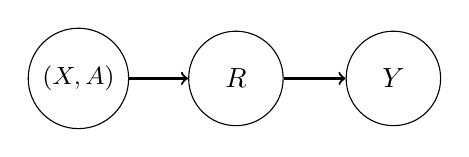
\begin{tikzpicture}

\node[circle,draw, minimum size=1.2cm] (R0) at (0,0) {\begin{small}$(X, A)$\end{small}
};
\node[circle,draw, minimum size=1.2cm] (R1) at (2,0) {$R$};
\node[circle,draw, minimum size=1.2cm] (Y) at (4,0) {$Y$};

\path[->, thick] (R0) edge (R1);
\path[->, thick] (R1) edge (Y);

\end{tikzpicture}
\caption{Bayesian network corresponding to Assumption \ref{assum:indep-general}.}
\label{fig:embedding_single}
% \vspace{-0.5cm}
% \end{wrapfigure}
\end{figure}
As illustrated in Figure \ref{fig:embedding_single}, Assumption \ref{assum:indep-general} means that the embedding $R$ fully mediates every possible effect of $(X, A)$ on $Y$. The generalised MIPS estimator $\hat{\theta}_{\textup{G-MIPS}}$ of target policy value, $\Etar[Y]$, is defined as
\[
\hat{\theta}_{\textup{G-MIPS}} \coloneqq \frac{1}{n}\sum_{i=1}^n \frac{\ptar(r_i)}{\pbeh(r_i)}\, y_i,
\]
where $\pbeh(r)$ denote the density of $R$ under the behaviour policy (likewise for $\ptar(r)$). Under assumption \ref{assum:indep-general}, $\hat{\theta}_{\textup{G-MIPS}}$ provides an unbiased estimator of target policy value. 
Similar to Lemma \ref{lemma:weights-est}, the density ratio $\frac{\ptar(r)}{\pbeh(r)}$ can be estimated by solving the regression problem
\begin{align}
    \arg \min_f \Ebeh \left(\frac{\tar(A\mid X)}{\beh(A\mid X)} - f\left(R\right)\right)^2. \label{eq:embedding-ratio-estimation}
\end{align}

\subsection{Variance reduction of G-MIPS estimator}\label{app:gmips-var-reduction}
By only considering the shift in the embedding $R$, the G-MIPS estimator achieves a lower variance relative to the vanilla IPW estimator. The following result, which is a straightforward extension of \cite[Theorem 3.6]{saito2022off}, formalises this.

\begin{proposition}[Variance reduction of G-MIPS]\label{prop:mips_var_reduction}
    When the ratios $\rho(a, x)$ and $\frac{\ptar(r)}{\pbeh(r)}$ are known exactly then under Assumption \ref{assum:indep-general}, we have that $\Ebeh[\thetaipw] = \Ebeh[\hat{\theta}_{\textup{G-MIPS}}] = \Etar[Y]$. Moreover,
\begin{align*}
     \Vbeh[\thetaipw] - \Vbeh[\hat{\theta}_{\textup{G-MIPS}}]
    \geq \frac{1}{n}\Ebeh \left[ \E[Y^2\mid R] \Vbeh[\rho(A, X)\mid R] \right] \geq 0.
\end{align*}
\end{proposition}

\begin{proof}[Proof of Proposition \ref{prop:mips_var_reduction}]
The following proof, which is included for completeness, is a straightforward extension of \cite[Theorem 3.6]{saito2022off}. 
\begin{align*}
    &n (\Vbeh[\thetaipw] - \Vbeh[\hat{\theta}_{\textup{MIPS}}])\\
    &\quad= \Vbeh\left[\frac{\tar(A|X)}{\beh(A|X)}\,Y\right] - \Vbeh\left[\frac{\ptar(R)}{\pbeh(R)}\,Y \right]\\
     &\quad= \Vbeh\left[\Ebeh\left[\frac{\tar(A|X)}{\beh(A|X)}\,Y \Bigg| R\right]\right] + \Ebeh\left[ \Vbeh\left[\frac{\tar(A|X)}{\beh(A|X)}\,Y\Bigg| R \right]\right] - \Vbeh\left[\Ebeh\left[ \frac{\ptar(R)}{\pbeh(R)}\,Y \Bigg| R\right]\right]\\
     &\qquad- \Ebeh\left[\Vbeh\left[ \frac{\ptar(R)}{\pbeh(R)}\,Y \Bigg| R\right]\right]
\end{align*}
Now using the conditional independence Assumption \ref{assum:indep-general}, the first term on the RHS above becomes,
\begin{align*}
    \Vbeh\left[\Ebeh\left[\frac{\tar(A|X)}{\beh(A|X)}\,Y \Bigg| R\right]\right] &= \Vbeh\left[\Ebeh\left[\frac{\tar(A|X)}{\beh(A|X)}\Bigg| R\right]\,\Ebeh\left[Y | R\right]\right]\\
    &= \Vbeh\left[\frac{\ptar(R)}{\pbeh(R)}\,\Ebeh\left[Y | R\right]\right],
\end{align*}
where in the last step above we use the fact that
\begin{align*}
    \Ebeh\left[\frac{\tar(A|X)}{\beh(A|X)}\Bigg| R\right] = \frac{\ptar(R)}{\pbeh(R)}.
\end{align*}
Putting this together, we get that
\begin{align}
    &n (\Vbeh[\thetaipw] - \Vbeh[\hat{\theta}_{\textup{MIPS}}]) \nonumber\\ 
    &\quad= \Ebeh\left[ \Vbeh\left[\frac{\tar(A|X)}{\beh(A|X)}\,Y\Bigg| R \right]\right] - \Ebeh\left[\Vbeh\left[ \frac{\ptar(R)}{\pbeh(R)}\,Y \Bigg| R\right]\right]. \label{eq:variance-difference}
\end{align}
Since we have that 
\begin{align*}
    \Ebeh\left[\frac{\tar(A|X)}{\beh(A|X)}\,Y\Bigg| R \right] = \Ebeh\left[\frac{\tar(A|X)}{\beh(A|X)}\Bigg| R \right]\,\Ebeh\left[Y| R \right] = \frac{\ptar(R)}{\pbeh(R)}\,\Ebeh\left[Y| R \right],
\end{align*}
Eq. \eqref{eq:variance-difference} becomes,
\begin{align*}
    &\Ebeh\left[ \Vbeh\left[\frac{\tar(A|X)}{\beh(A|X)}\,Y\Bigg| R \right]\right] - \Ebeh\left[\Vbeh\left[ \frac{\ptar(R)}{\pbeh(R)}\,Y \Bigg| R\right]\right] \\
    &\quad= \Ebeh\left[ \Ebeh\left[ \left(\frac{\tar(A|X)}{\beh(A|X)}\,Y \right)^2\Bigg| R  \right] - \Ebeh\left[ \left(\frac{\ptar(R)}{\pbeh(R)}\,Y \right)^2\Bigg| R \right] \right]\\
    &\quad= \Ebeh\left[ \Ebeh\left[ \left(\frac{\tar(A|X)}{\beh(A|X)} \right)^2 \Bigg| R  \right] \, \Ebeh\left[Y^2 | R  \right] - \left(\frac{\ptar(R)}{\pbeh(R)}\right)^2\,\Ebeh\left[Y^2 | R \right] \right]\\
    &\quad= \Ebeh\left[\Ebeh\left[Y^2 | R \right]\, \left( \Ebeh\left[ \left(\frac{\tar(A|X)}{\beh(A|X)} \right)^2 \Bigg| R  \right] - \left(\Ebeh\left[ \frac{\tar(A|X)}{\beh(A|X)} \Bigg| R  \right]\right)^2\, \right) \right]\\
    &\quad=\Ebeh\left[\Ebeh\left[Y^2 | R \right]\, \Vbeh\left[\frac{\tar(A|X)}{\beh(A|X)} \Bigg| R \right]\right].
\end{align*}
\end{proof}

\paragraph{Intuition}
Here, $R$ contains all relevant information regarding the outcome $Y$. Moreover, intuitively $R$ can be thought of as the state obtained by `filtering out' relevant information about $Y$ from $(X, A)$. Therefore, $R$ contains less `redundant' information regarding the outcome $Y$ as compared to the covariate-action pair $(X, A)$. As a result, the G-MIPS estimator which only considers the shift in the marginal distribution of $R$ due to the policy shift is more efficient than the IPW estimator, which considers the shift in the joint distribution of $(X, A)$ instead.
In fact, as the amount of `redundant' information regarding $Y$ decreases in the embedding $R$, the G-MIPS estimator becomes increasingly efficient with decreasing variance. We formalise this as follows:
\begin{assumption}\label{assum:two-embeddings}
    Assume there exist embeddings $R^{(1)}, R^{(2)}$ of the covariate-action pair $(X, A)$, with Bayesian network shown in Figure \ref{fig:embedding_double}. 
    This corresponds to the following conditional independence assumptions:
    \[
    R^{(2)} \indep (X, A) \mid R^{(1)}, \qquad \textup{and} \qquad Y \indep (R^{(1)}, X, A) \mid R^{(2)}.
    \]
\end{assumption}
\begin{figure}[h!]
\centering
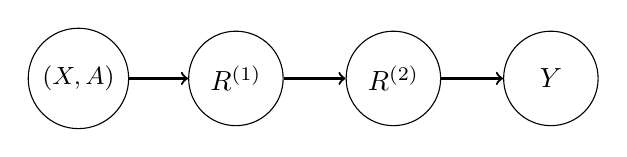
\begin{tikzpicture}

\node[circle,draw, minimum size=1.2cm] (R0) at (0,0) {\begin{small}$(X, A)$\end{small}};
\node[circle,draw, minimum size=1.2cm] (R1) at (2,0) {$R^{(1)}$};
\node[circle,draw, minimum size=1.2cm] (R2) at (4,0) {$R^{(2)}$};
\node[circle,draw, minimum size=1.2cm] (Y) at (6,0) {$Y$};

\path[->, thick] (R0) edge (R1);
\path[->, thick] (R1) edge (R2);
\path[->, thick] (R2) edge (Y);

\end{tikzpicture}
\caption{Bayesian network corresponding to Assumption \ref{assum:two-embeddings}.}
\label{fig:embedding_double}
\end{figure}  
% Here, $R^{(2)}$ can be thought of as the embedding obtained by `filtering out' relevant information about $Y$ from $R^{(1)}$, and as such $R^{(2)}$ contains less redundant information about $Y$ as compared to $R^{(1)}$. 
We can define G-MIPS estimators for these embeddings to obtain unbiased OPE estimators under Assumption \ref{assum:two-embeddings} as follows:
\[    \hat{\theta}^{(j)}_{\textup{G-MIPS}} \coloneqq \frac{1}{n}\sum_{i=1}^n \frac{\ptar(r_i^{(j)})}{\pbeh(r_i^{(j)})}\, y_i,
\]
for $j\in \{1, 2\}$. Here, $\frac{\ptar(r^{(j)})}{\pbeh(r^{(j)})}$ is the ratio of marginal densities of $R^{(j)}$ under target and behaviour policies. 
We next show that the variance of $\hat{\theta}^{(j)}_{\textup{G-MIPS}}$ decreases with increasing $j$.
\begin{proposition}\label{prop:mips_generalised}
    When the ratios $\rho(a, x)$, $w(y)$ and $\frac{\ptar(r^{(j)})}{\pbeh(r^{(j)})}$ are known exactly for $j \in \{1, 2\}$, then under Assumption \ref{assum:two-embeddings} we get that
    \[
    \Ebeh[\thetaipw] = \Ebeh[\hat{\theta}^{(1)}_{\textup{G-MIPS}}] = \Ebeh[\hat{\theta}^{(2)}_{\textup{G-MIPS}}] = \Ebeh[\thetamr] = \Etar[Y].
    \]
    Moreover, 
    \[
    \Vbeh[\thetaipw] \geq \Vbeh[\hat{\theta}^{(1)}_{\textup{G-MIPS}}] \geq  \Vbeh[\hat{\theta}^{(2)}_{\textup{G-MIPS}}] \geq \Vbeh[\thetamr].
    \]
\end{proposition}
\begin{proof}[Proof of Proposition \ref{prop:mips_generalised}]
    First, we prove that the G-MIPS estimators are unbiased using induction on $j$. We define $R^{(0)} \coloneqq (X, A)$ and $\hat{\theta}^{(0)}_{\textup{G-MIPS}}$ defined as
    \[
    \hat{\theta}^{(0)}_{\textup{G-MIPS}} \coloneqq \frac{1}{n}\sum_{i=1}^n \frac{\ptar(r_i^{(0)})}{\pbeh(r_i^{(0)})}\, y_i,
    \]
    recovers the IPW estimator $\thetaipw$. When $j=0$, we know that $\hat{\theta}^{(0)}_{\textup{G-MIPS}} = \thetaipw$ is unbiased. 
    Now, assume that $\Ebeh[\hat{\theta}^{(j)}_{\textup{G-MIPS}}] = \Etar[Y]$.

    Conditional on $R^{(j)}$, $R^{(j+1)}$ does not depend on the policy. Therefore, 
    \begin{align*}
        \frac{\ptar(r^{(j)})}{\pbeh(r^{(j)})} = \frac{\ptar(r^{(j)})\,p(r^{(j+1)}\mid r^{(j)}) }{\pbeh(r^{(j)})\,p(r^{(j+1)}\mid r^{(j)})} = \frac{\ptar(r^{(j)}, r^{(j+1)})}{\pbeh(r^{(j)}, r^{(j+1)})}.
    \end{align*}
    And therefore,
    \begin{align*}
        \frac{\ptar(r^{(j+1)})}{\pbeh(r^{(j+1)})} &= \int_{r^{(j)}} \frac{\ptar(r^{(j)}, r^{(j+1)})}{\pbeh(r^{(j)}, r^{(j+1)})} \, \pbeh(r^{(j)} \mid r^{(j+1)}) \,\mathrm{d} r^{(j)}\\ 
        &= \int_{r^{(j)}} \frac{\ptar(r^{(j)})}{\pbeh(r^{(j)})} \,\pbeh(r^{(j)} \mid r^{(j+1)}) \,\mathrm{d} r^{(j)}\\ 
        &= \Ebeh\left[\frac{\ptar(R^{(j)})}{\pbeh(R^{(j)})} \Bigg|  R^{(j+1)}=r^{(j+1)}\right].
    \end{align*}
    Using this and the fact that $R^{(j)}\indep Y \mid R^{(j+1)}$, we get that
    \begin{align*}
        \Ebeh\left[\hat{\theta}^{(j+1)}_{\textup{G-MIPS}} \right] &= \Ebeh\left[\frac{\ptar(R^{(j+1)})}{\pbeh(R^{(j+1)})}\, Y \right]\\
        &= \Ebeh\left[\frac{\ptar(R^{(j+1)})}{\pbeh(R^{(j+1)})}\, \Ebeh[Y| R^{(j+1)}] \right]\\
        &= \Ebeh\left[\Ebeh\left[\frac{\ptar(R^{(j)})}{\pbeh(R^{(j)})} \Bigg|  R^{(j+1)}\right]\, \Ebeh[Y| R^{(j+1)}] \right] \\
        &= \Ebeh\left[\Ebeh\left[\frac{\ptar(R^{(j)})}{\pbeh(R^{(j)})} \, Y \Bigg|  R^{(j+1)}\right]\right]\\
        &= \Ebeh\left[ \frac{\ptar(R^{(j)})}{\pbeh(R^{(j)})} \, Y \right]\\
        &= \Ebeh\left[\hat{\theta}^{(j)}_{\textup{G-MIPS}} \right] = \Etar[Y].
    \end{align*}
    Next, to prove the variance result we consider the difference
    \begin{align*}
        &\Vbeh[\hat{\theta}^{(j)}_{\textup{G-MIPS}}] - \Vbeh[\hat{\theta}^{(j+1)}_{\textup{G-MIPS}}] \\
        &= \frac{1}{n}\left(\Vbeh\left[\frac{\ptar(R^{(j)})}{\pbeh(R^{(j)})}\, Y\right] - \Vbeh\left[\frac{\ptar(R^{(j+1)})}{\pbeh(R^{(j+1)})}\, Y\right]\right) \\
        % &= \frac{1}{n}\left(\Vbeh\left[\frac{\ptar(R^{(j)})}{\pbeh(R^{(j)})}\, Y\right] - \Vbeh\left[\Ebeh\left[\frac{\ptar(R^{(j)})}{\pbeh(R^{(j)})} \Bigg|  R^{(j+1)}\right]\, Y\right]\right)\\
        &= \frac{1}{n}\Bigg(\Vbeh\left[ \Ebeh\left[\frac{\ptar(R^{(j)})}{\pbeh(R^{(j)})}\, Y \Bigg| R^{(j+1)} \right] \right] + \Ebeh\left[ \Vbeh\left[\frac{\ptar(R^{(j)})}{\pbeh(R^{(j)})}\, Y \Bigg| R^{(j+1)} \right] \right] \\
        &\qquad- \Vbeh\left[\frac{\ptar(R^{(j+1)})}{\pbeh(R^{(j+1)})}\, \Ebeh[Y\mid R^{(j+1)}]\right] - \Ebeh \left[\left(\frac{\ptar(R^{(j+1)})}{\pbeh(R^{(j+1)})}\right)^2\,\Vbeh[Y\mid R^{(j+1)}] \right] \Bigg)
    \end{align*}
    where in the last step we use the law of total variance. Now, using the fact that $R^{(j)}\indep Y \mid R^{(j+1)}$, we can rewrite the expression above as
    \begin{align*}
        &= \frac{1}{n}\Bigg(\Vbeh\left[ \Ebeh\left[\frac{\ptar(R^{(j)})}{\pbeh(R^{(j)})}\Bigg| R^{(j+1)} \right]\, \Ebeh[Y | R^{(j+1)} ] \right] + \Ebeh\left[ \Vbeh\left[\frac{\ptar(R^{(j)})}{\pbeh(R^{(j)})}\, Y \Bigg| R^{(j+1)} \right] \right] \\
        &\qquad- \Vbeh\left[\frac{\ptar(R^{(j+1)})}{\pbeh(R^{(j+1)})}\, \Ebeh[Y\mid R^{(j+1)}]\right] - \Ebeh \left[\left(\frac{\ptar(R^{(j+1)})}{\pbeh(R^{(j+1)})}\right)^2\,\Vbeh[Y\mid R^{(j+1)}] \right] \Bigg)\\
        &= \frac{1}{n}\Bigg( \Ebeh\left[ \Vbeh\left[\frac{\ptar(R^{(j)})}{\pbeh(R^{(j)})}\, Y \Bigg| R^{(j+1)} \right] \right] - \Ebeh \left[\left(\frac{\ptar(R^{(j+1)})}{\pbeh(R^{(j+1)})}\right)^2\,\Vbeh[Y\mid R^{(j+1)}] \right]\Bigg).
    \end{align*}
    Moreover, again using the conditional independence $R^{(j)}\indep Y \mid R^{(j+1)}$, we can expand the first term in the expression above as follows:
    % \begin{align*}
    %     \Vbeh\left[ \Ebeh\left[\frac{\ptar(R^{(j)})}{\pbeh(R^{(j)})}\, Y \Bigg| R^{(j+1)} \right] \right] &=
    %     \Vbeh\left[ \Ebeh\left[\frac{\ptar(R^{(j)})}{\pbeh(R^{(j)})}\Bigg| R^{(j+1)}\right]\, \Ebeh\left[Y | R^{(j+1)} \right] \right]\\
    %     &= \Vbeh\left[ \frac{\ptar(R^{(j+1)})}{\pbeh(R^{(j+1)})}\, \Ebeh\left[Y | R^{(j+1)} \right]\right]
    % \end{align*}
    \begin{align*}
        \Ebeh\left[ \Vbeh\left[\frac{\ptar(R^{(j)})}{\pbeh(R^{(j)})}\, Y \Bigg| R^{(j+1)} \right] \right] &=
        \Ebeh\Bigg[ \Ebeh\left[\frac{\ptar^2(R^{(j)})}{\pbeh^2(R^{(j)})} \Bigg| R^{(j+1)} \right]\,\Ebeh[Y^2 | R^{(j+1)}] \\
        &\qquad- \left(\Ebeh\left[\frac{\ptar(R^{(j)})}{\pbeh(R^{(j)})} \Bigg| R^{(j+1)} \right] \Ebeh[Y | R^{(j+1)}] \right)^2 \Bigg]\\
        &\geq 
        \Ebeh\Bigg[ \left(\Ebeh\left[\frac{\ptar(R^{(j)})}{\pbeh(R^{(j)})} \Bigg| R^{(j+1)} \right]\right)^2 \,\Ebeh[Y^2 | R^{(j+1)}] \\
        &\qquad- \left(\frac{\ptar(R^{(j+1)})}{\pbeh(R^{(j+1)})} \Ebeh[Y | R^{(j+1)}] \right)^2 \Bigg]\\
        &= \Ebeh\Bigg[ \left(\frac{\ptar(R^{(j+1)})}{\pbeh(R^{(j+1)})}\right)^2 \, \Vbeh[Y\mid R^{(j+1)}] \Bigg].
    \end{align*}
    Here, to get the inequality above, we use the fact that $\E[X^2] \geq (\E[X])^2$. Putting this together, we get that $\Vbeh[\hat{\theta}^{(j)}_{\textup{G-MIPS}}] - \Vbeh[\hat{\theta}^{(j+1)}_{\textup{G-MIPS}}] \geq 0$.

    Moreover, the result $\Vbeh[\hat{\theta}^{(2)}_{\textup{G-MIPS}}] \geq \Vbeh[\thetamr]$ follows straightforwardly from above by defining $R^{(3)} \coloneqq Y$. Then, the embeddings satisfy the causal structure 
    \[
    R^{(0)} \rightarrow R^{(1)} \rightarrow R^{(2)}  \rightarrow R^{(3)} \rightarrow Y.
    \]
    Using the result above, we know that $\Vbeh[\hat{\theta}^{(2)}_{\textup{G-MIPS}}] \geq \Vbeh[\hat{\theta}^{(3)}_{\textup{G-MIPS}}]$. But now it is straightforward to see that $\hat{\theta}^{(3)}_{\textup{G-MIPS}} = \thetamr$, and the result follows.
\end{proof}

\paragraph{Intuition}
Here, $R^{(j+1)}$ can be thought of as the embedding obtained by `filtering out' relevant information about $Y$ from $R^{(j)}$. As such, the amount of `redundant' information regarding the outcome $Y$ decreases successively along the sequence $R^{(0)} (\coloneqq (X, A)), R^{(1)}, R^{(2)}$. As a result, the G-MIPS estimators which only consider the shift in the marginal distributions of $R^{(j)}$ due to policy shift become increasingly efficient with decreasing variance as $j$ increases. Define the representation $R^{(3)} \coloneqq Y$, then the corresponding G-MIPS estimator reduces to the MR estimator, i.e., $\hat{\theta}^{(3)}_{\textup{G-MIPS}} = \thetamr$. Moreover, this estimator has minimum variance among all the G-MIPS estimators $\{\hat{\theta}^{(j)}_{\textup{G-MIPS}}\}_{0\leq j\leq k}$, as the representation $R^{(3)}$ contains precisely the least amount of information necessary to obtain the outcome $Y$. In other words, $Y$ itself serves as the `best embedding' of covariate-action pair $R^{(0)}$ which contains all relevant information regarding $Y$. We verify this empirically in Appendix \ref{subsec:mips-empirical} by reproducing the experimental setup in \cite{saito2022off} along with the MR baseline. Additionally, the MR estimator does not rely on assumptions like \ref{assum:indep-general} for unbiasedness. 

In addition to this, solving the regression problem in Eq. \eqref{eq:embedding-ratio-estimation} will typically be more difficult when $R$ is higher dimensional (as is likely to be the case for many choices of embeddings $R$), leading to high bias. In contrast, for MR the embedding $R=Y$ is one dimensional and therefore the regression problem is significantly easier to solve and yields lower bias. Our empirical results in Appendix \ref{app:experiments} confirm this.

\subsection{Doubly robust G-MIPS estimators}
Consider the setup for the G-MIPS estimator shown in Figure \ref{fig:embedding_single}. In this case, we can derive a doubly robust extension of the G-MIPS estimator, denoted as GM-DR, which uses an estimate of the conditional mean $\tilde{\mu}(r) \approx \E[Y\mid R=r]$ as a control variate to decrease the variance of G-MIPS estimator. This can be explicitly written as follows:
\begin{align}
\thetagmdr \coloneqq \frac{1}{n} \sum_{i=1}^n \frac{\ptar(r_i)}{\pbeh(r_i)}\,(y_i - \tilde{\mu}(r_i)) + \tilde{\eta}(\tar). \label{eq:gmips-dr}    
\end{align}
where $\tilde{\eta}(\tar) = \frac{1}{n} \sum_{i=1}^n \sum_{r' \in \mathcal{R}} \tilde{\mu}(r') \, \ptar(r' \mid x_i)$ is the analogue of the direct method. Here, $\mathcal{R}$ denotes the space of the possible of the representations $R$\footnote{the $\sum_{r' \in \mathcal{R}}$ can be replaced with $\int_{r' \in \mathcal{R}} \mathrm{d}r'$ when $\mathcal{R}$ is continuous}. Moreover, given the density $p(r \mid x, a)$, we can compute $\ptar(r\mid x)$ using
\[
\ptar(r\mid x) = \sum_{a' \in \Aspace} p(r \mid x, a')\,\tar(a'\mid x).
\]
It is straightforward to extend ideas from \cite{dudik2014doubly} to show that estimator $\thetagmdr$ is doubly robust in that it will yield accurate value estimates if either the importance weights $\frac{\ptar(r)}{\pbeh(r)}$ or the outcome model $\tilde{\mu}(r)$ is well estimated. 

\paragraph{There is no analogous DR extension of the MR estimator}
A consequence of considering the embedding $R=Y$ (as in MR) is that in this case we do not have an analogous doubly robust extension as above. To see why this is the case, note that when $R=Y$, we get that $\tilde{\mu}(r) = \E[Y\mid R=r] = \E[Y\mid Y=y] = y$. If we substitute this $\tilde{\mu}(r)$ in \eqref{eq:gmips-dr}, we are simply left with $\tilde{\eta}(\tar)$ on the right hand side (as the first term cancels out). This means that the resulting estimator does not retain the doubly robust nature as we no longer obtain an accurate estimate if either the outcome model or the importance ratios are well estimated.
% Additionally, $\tilde{\eta}(\tar)$ is an accurate estimate of the policy estimate only in the case when we have a good estimate of $\ptar(y\mid x)$.
% This is a non-trivial distribution to estimate as we do not have reward samples from the target distribution. Moreover, this also means that the resulting estimator does not retain the doubly robust nature as we no longer obtain an accurate estimate if either the outcome model or the importance ratios are well estimated.


% \newpage
\section{Application to causal inference}\label{app:causal-inference}
In this section, we investigate the application of the MR estimator for the estimation of average treatment effect (ATE). In this setting, we suppose that $\Aspace = \{0, 1\}$, and the goal is to estimate ATE defined as follows:
\[
\ate \coloneqq \E[Y(1)-Y(0)]
\]
Here, we use the potential outcomes notation \citep{robins1986new} to denote the outcome under a deterministic policy $\tar(a'\mid x) = \mathbbm{1}(a'=a)$ as $Y(a)$. 

Specifically, the IPW estimator applied to ATE estimation yields:
\[
\ateipw = \frac{1}{n} \sum_{i=1}^n \rho_{\ate}(a_i, x_i) \times y_i,
\]
where 
\[
\rho_{\ate}(a, x) \coloneqq \frac{\mathbbm{1}(a=1) - \mathbbm{1}(a=0)}{\beh (a|x)}.
\]
Similarly, the MR estimator can be written as
\[
\atemr = \frac{1}{n}\sum_{i=1}^n w_{\ate}(y_i)\times y_i, 
\]
where
\[
w_{\ate}(y) = \frac{p_{\pi^{(1)}}(y) - p_{\pi^{(0)}}(y)}{\pbeh(y)},
\] 
and $\pi^{(a)}(a'\mid x) \coloneqq \mathbbm{1}(a'=a)$ for $a\in \{0,1\}$.

Again, using the fact that $w_{\ate}(Y) \eqas \E[\rho_{\ate}(A, X)\mid Y]$, we can obtain $w_{\ate}$ by minimising a simple mean-squared loss:
\begin{align*}
    w_{\ate} =\arg \min_{f} \Ebeh \Big[\frac{\mathbbm{1}(A=1)- \mathbbm{1}(A=0)}{\beh (A|X)}-f(Y)\Big]^2.
\end{align*}
\begin{proposition}[Variance comparison with IPW ATE estimator]\label{prop:ate_variance}
When the weights $\rho_{\ate}(a, x)$ and $w_{\ate}(y)$ are known exactly, we have that $\V[\atemr] \leq \V[\ateipw]$. Specifically,
\begin{align*}
    \V[\ateipw] - \V[\atemr] = \frac{1}{n}\E\left[ \V\left[\rho_{\ate}(A, X) | Y \right]\,Y^2 \right] \geq 0.
\end{align*}
\end{proposition}
\begin{proof}[Proof of Proposition \ref{prop:ate_variance}] We have
\begin{align}
    \V[\ateipw] - \V[\atemr] &= \frac{1}{n}\left( \V[\rho_{\ate}(A, X)\, Y] - \V[w_{\ate}(Y)\,Y] \right). \label{eq:variance_ate_ipw_minus_mr}
\end{align}
Using the tower law of variance, we get that
\begin{align*}
    \V[\rho_{\ate}(A, X)\, Y] 
    &= \V[\E[\rho_{\ate}(A, X)\,  Y\mid Y]] + \E[\V[\rho_{\ate}(A, X)\, Y\mid Y]]\\
    &= \V[\E[\rho_{\ate}(A, X)\mid Y]\,  Y] + \E[\V[\rho_{\ate}(A, X)\mid Y]\,Y^2]\\
    &= \V[w_{\ate}(Y)\,Y] + \E[\V[\rho_{\ate}(A, X)\mid Y]\,Y^2].
\end{align*}
Putting this together with \eqref{eq:variance_ate_ipw_minus_mr} we obtain,
\begin{align*}
    \V[\ateipw] - \V[\atemr] &= \frac{1}{n} \E[\V[\rho_{\ate}(A, X)\mid Y]\,Y^2],
\end{align*}
which straightforwardly leads to the result.
\end{proof}

Given the above definitions, the IPW estimator for $\E[Y(a)]$ would only consider datapoints with $A=a$, as it weights the samples using the policy ratios $\mathbbm{1}(A=a)/\beh(A|X)$ which are only non-zero when $A=a$. 
This is however not the case with the MR estimator, as it uses the weights $\ptar(Y)/\pbeh(Y)$ which are not necessarily zero for $A\neq a$. Therefore, MR uses all evaluation datapoints $\D$ when estimating $\E[Y(a)]$. The MR estimator therefore leads to a more efficient use of evaluation data in this example. 
% The MR estimator, on the other hand, yields an unweighted average since $\ptar(Y)/\pbeh(Y)=1$, and more importantly, uses all datapoints when estimating $\E[Y(1)]$. The MR estimator therefore leads to a more efficient use of data in this example. 
% \faaiz{consider the comparison against DR estimator}

Likewise, the doubly robust (DR) estimator applied to ATE estimation yields,
\begin{align*}
    \atedr \coloneqq \frac{1}{n} \sum_{i=1}^n \rho_{\ate}(a_i, x_i)\,\left(y_i - \hat{\mu}(a_i, x_i)\right) + \frac{1}{n} \sum_{i=1}^n \left( \hat{\mu}(1, x_i)-  \hat{\mu}(0, x_i)\right),
\end{align*}
where $\hat{\mu}(a, x)\approx \E[Y\mid X=x, A=a]$. 
Like in classical off-policy evaluation, DR yields an accurate estimator of ATE when either the weights $\rho_{\ate}(a, x)$ or the outcome model i.e., $\hat{\mu}(a, x) = \E[Y\mid X=x, A=a]$, are well estimated.
However, despite this doubly robust nature of the estimator, we can show that the variance of the DR estimator may be higher than that of the MR estimator in many cases. The following result formalises this variance comparison between the DR and MR estimators, and is analogous to the result in Proposition \ref{prop:var_dr} derived for classical off-policy evaluation. 
\begin{proposition}[Variance comparison with DR ATE estimator]\label{prop:ate_var_dr}
    When the weights $\rho_{\ate}(a, x)$ and $w_{\ate}(y)$ are known exactly,
    \begin{align*}
    &\V[\atedr] - \V[\atemr]\\
    &\qquad \qquad \qquad \geq \frac{1}{n}\E \left[ \V\left[ \rho_\ate(A, X)\,Y \mid Y \right] -  \V\left[ \rho_\ate(A, X)\mu(A, X) \mid X \right] \right],
\end{align*}
where $\mu(A, X) \coloneqq \E[Y\mid X, A]$.
\end{proposition}

\begin{proof}[Proof of Proposition \ref{prop:ate_var_dr}]
Using the law of total variance, we get that
\begin{align*}
    n\,\V[\atedr] &= \V[\rho_\ate(A, X)\,(Y -\hat{\mu}(A, X)) + (\hat{\mu}(1, X) - \hat{\mu}(0, X))]\\
    &= \V[ \E[\rho_\ate(A, X)\,(Y -\hat{\mu}(A, X)) + (\hat{\mu}(1, X) - \hat{\mu}(0, X))\mid X, A]] \\
    &\qquad+ \E[\V[\rho_\ate(A, X)\,(Y -\hat{\mu}(A, X)) + (\hat{\mu}(1, X) - \hat{\mu}(0, X))\mid X, A]]\\
    &= \V[ \rho_\ate(A, X)\,(\mu(A, X) -\hat{\mu}(A, X)) + (\hat{\mu}(1, X) - \hat{\mu}(0, X))]\\
    &\qquad+ \E[\rho^2_\ate(A, X)\V[Y\mid X, A]].
\end{align*}
    Again, using the law of total variance we can rewrite the first term on the RHS above as,
    \begin{align*}
        &\V[ \rho_\ate(A, X)\,(\mu(A, X) -\hat{\mu}(A, X)) + (\hat{\mu}(1, X) - \hat{\mu}(0, X))]\\
        &\quad= \V[\E[ \rho_\ate(A, X)\,(\mu(A, X) -\hat{\mu}(A, X)) + (\hat{\mu}(1, X) - \hat{\mu}(0, X))\mid  X]] \\
        &\qquad+ \E[\V[ \rho_\ate(A, X)\,(\mu(A, X) -\hat{\mu}(A, X)) + (\hat{\mu}(1, X) - \hat{\mu}(0, X))\mid  X]] \\
        &\quad\geq  \V[\E[ \rho_\ate(A, X)\,(\mu(A, X) -\hat{\mu}(A, X)) + (\hat{\mu}(1, X) - \hat{\mu}(0, X))\mid  X]]\\
        &\quad=  \V[\E[ \rho_\ate(A, X)\,(\mu(A, X) -\hat{\mu}(A, X)) + \rho_\ate(A, X)\,\hat{\mu}(A, X)\mid  X]]\\
        &\quad=  \V[\E[ \rho_\ate(A, X)\,\mu(A, X)\mid  X]],
    \end{align*}
    where, in the second last step above we use the fact that 
    \[
    \E[\rho_\ate(A, X)\,\hat{\mu}(A, X)\mid  X] = \hat{\mu}(1, X) - \hat{\mu}(0, X).
    \]

    Putting this together, we get that
    \begin{align*}
        n\,\V[\atedr] \geq \V[\E[ \rho_\ate(A, X)\,\mu(A, X)\mid  X]] + \E[\rho^2_\ate(A, X)\V[Y\mid X, A]].
    \end{align*}
    Therefore, 
    \begin{align*}
        &n\,(\V[\atedr] - \V[\atemr]) \\
        &\quad\geq \V[\E[ \rho_\ate(A, X)\,\mu(A, X)\mid  X]] + \E[\rho^2_\ate(A, X)\V[Y\mid X, A]] - \V[w_\ate(Y)\,Y]\\
        &\quad= \V[\E[ \rho_\ate(A, X)\,\mu(A, X)\mid  X]] + \E[\V[\rho_\ate(A, X)\,Y\mid X, A]] - \V[w_\ate(Y)\,Y]\\
        &\quad= \V[\E[ \rho_\ate(A, X)\,\mu(A, X)\mid  X]] + \V[\rho_\ate(A, X)\, Y] - \V[\E[\rho_\ate(A, X)\,Y\mid X, A]]\\
        &\qquad- \V[w_\ate(Y)\,Y]\\
        &\quad= \V[\E[ \rho_\ate(A, X)\,\mu(A, X)\mid  X]] + \V[\E[\rho_\ate(A, X)\mid Y]\, Y] + \E[\V[\rho_\ate(A, X)\mid Y]\,Y^2]\\
        &\qquad- \V[\E[\rho_\ate(A, X)\,Y\mid X, A]]- \V[w_\ate(Y)\,Y]\\
        &\quad= \V[\E[ \rho_\ate(A, X)\,\mu(A, X)\mid  X]] + \V[w_\ate(Y)\, Y] + \E[\V[\rho_\ate(A, X)\mid Y]\,Y^2]\\
        &\qquad- \V[\E[\rho_\ate(A, X)\,Y\mid X, A]]- \V[w_\ate(Y)\,Y]\\
        &\quad= \V[\E[ \rho_\ate(A, X)\,\mu(A, X)\mid  X]]- \V[\E[\rho_\ate(A, X)\,Y\mid X, A]] + \E[\V[\rho_\ate(A, X)\mid Y]\,Y^2]\\
        &\quad= \V[\rho_\ate(A, X)\,\mu(A, X)] - \E[\V[\rho_\ate(A, X)\,\mu(A, X)\mid  X]] - \V[\rho_\ate(A, X)\,\mu(A, X)]\\
        &\qquad+ \E[\V[\rho_\ate(A, X)\mid Y]\,Y^2]\\
        &\quad= \E \left[ \V\left[ \rho_\ate(A, X) \mid Y \right]\, Y^2 -  \V\left[ \rho_\ate(A, X)\mu(A, X) \mid X \right] \right].
        % &\quad\geq \V[\E[ \rho_\ate(A, X)\,\mu(A, X)\mid  X]]- \V[\rho_\ate(A, X)\,\mu(A, X)] + \E[\V[\rho_\ate(A, X)\mid Y]\,Y^2]
    \end{align*}
\end{proof}

Proposition \ref{prop:ate_var_dr} shows that if $\V\left[Y\, \rho_\ate(A, X) \mid Y \right]$ is greater than $\V\left[ \rho_\ate(A, X)\mu(A, X) \mid X \right]$ on average, the variance of the MR estimator will be less than that of the DR estimator. Intuitively, this is likely to happen when the dimension of context space $\Xspace$ is high because in this case, the conditional variance over $X$ and $A$, $\V\left[Y\, \rho_\ate(A, X) \mid Y \right]$ is likely to be greater than the conditional variance over $A$, $\V\left[ \rho_\ate(A, X)\mu(A, X) \mid X \right]$.

% \newpage
\section{Experimental Results}\label{app:experiments}
In this section, we provide additional experimental details for the results presented in the main text. We also include extensive experimental results to provide further empirical evidence in favour of the MR estimator. 

\paragraph{Computational details}
We ran our experiments on Intel(R) Xeon(R) CPU E5-2690 v4 @ 2.60GHz with 8GB RAM
per core. We were able to use 150 CPUs in parallel to iterate over different configurations and seeds.
However, we would like to note that for each run our algorithms only requires 1 CPU and at most 30 minutes to run as our neural networks are relatively small. Throughout our experiments, whenever the outcome $Y$ was continuous, we used a fully connected neural network with three hidden layers with 512, 256 and 32 nodes respectively (and ReLU activation function) to estimate the weights $\hat{w}(y)$. On the other hand, when the outcome is discrete we can directly estimate $\hat{w}(y) \approx \E[\hat{\rho}(A, X)\mid Y=y]$ by calculating the sample mean of $\hat{\rho}(A, X)$ on samples with $Y=y$. Additionally, for each configuration of parameters in our experiments, we ran experiments for 10 different seeds (in \{0, 1, \ldots, 9\}).

\subsection{Alternative methodology of estimating MR}
In addition to the OPE baselines like IPW, DM and DR estimators considered in the main text, we also include empirically investigate an alternative methodology of estimating MR.
% results for MR estimated using an alternative methodology. 
Below we describe this methodology, denoted as `MR (alt)', in greater detail:
\subsubsection{MR (alt)}\label{sec:alt-estimation-method}
Recall our definition of MR estimator:
\[
\thetamr \coloneqq \frac{1}{n} \sum_{i=1}^n w(y_i)\,y_i.
\]
In the main text, we propose estimating the weights $w(y)$ first and using this to estimate $\thetamr$ using the above expression. Alternatively, we can estimate $h(y) \coloneqq y\,w(y)$ using 
\begin{align*}
    h = \arg\min_{f} \, \Ebeh \left[ \Bigg(Y\,\frac{\tar(A|X)}{\beh (A|X)}-f(Y)\Bigg)^2\right].
\end{align*}
Subsequently, the MR estimator can be written as:
\[
\thetamr = \frac{1}{n}\sum_{i=1}^n h(y_i).
\]
We refer to this alternative methodology as `MR-alt' and compare it empirically against the original methodology (which we simply refer to as `MR'). 
In general, it is difficult to say which of the two methods will perform better. Intuitively speaking, in cases where the behaviour of the quantity $Y\,\frac{\tar(A|X)}{\beh (A|X)}$ with varying $Y$ is `smoother' than that of $\frac{\tar(A|X)}{\beh (A|X)}$, the alternative method is expected to perform better. Our empirical results in the next sections show that the relative performance of the two methods varies for different data generating mechanisms.

% \subsubsection{Switch-DR estimator}\faaiz{duplication of these definitions}
% The original DR estimator can still have a high variance when the importance weights are large due to a large policy shift. Switch-DR \cite{wang2017optimal} aims to circumvent this problem by switching to DM when the importance weights are large:
% \[
% \thetaswitch \coloneqq \frac{1}{n} \sum_{i=1}^n \rho(a_i, x_i)\,(y_i - \hat{\mu}(a_i, x_i))\ind(\rho(a_i, x_i) \leq \tau) + \hat{\eta}(\tar)
% \]
% where $\tau \geq 0$ is a hyperparameter, $\hat{\mu}(a, x) \approx \E[Y \mid x, a]$ is the outcome model, and 
% \[
% \hat{\eta}(\tar) = \frac{1}{n} \sum_{i=1}^n \sum_{a'\in \Aspace} \hat{\mu}(a', x_i) \tar(a'\mid x_i) \approx \E_{\tar}[\hat{\mu}(A, X)].
% \]

% \subsubsection{Doubly Robust with Optimal Shrinkage (DRos)}
% DRos proposed by \citep{su2020doubly} uses new weights $\hat{\rho}_\lambda(a_i, x_i)$ which directly minimises sharp bounds on the MSE of the resulting estimator,
% \[
% \thetadros \coloneqq \frac{1}{n} \sum_{i=1}^n \hat{\rho}_\lambda(a_i, x_i)\,(y_i - \hat{\mu}(a_i, x_i)) + \hat{\eta}(\tar),
% \]
% where $\lambda \geq 0$ is a pre-defined hyperparameter and $\hat{\rho}_\lambda$ is defined as
% \[
% \hat{\rho}_\lambda(a, x) \coloneqq \frac{\lambda}{\rho^2(a, x) + \lambda}\, \rho(a, x).
% \]
% When $\lambda = 0$, $\hat{\rho}_\lambda(a, x) = 0$ leads to DM, whereas as $\lambda \rightarrow \infty$, $\hat{\rho}_\lambda(a, x) \rightarrow \rho(a, x)$ leading to DR.

\subsection{Synthetic data experiments}\label{subsec:mips-empirical}
Here, we include additional experimental details for the synthetic data experiments presented in Section \ref{sec:exp-synth} for completeness. For this experiment, we use the same setup as the synthetic data experiment in \cite{saito2022off}, reproduced by reusing their code with minor modifications. 


% To verify the theoretical results in Section \ref{subsec:mips-comparison}, we empirically compare the MR estimator with the MIPS estimator. To do this, we reproduce the experimental setup for the synthetic data experiment in \cite{saito2022off} by reusing their code. Below, we include the experimental details for completeness. 

\paragraph{Setup}
Here, we sample the $d$-dimensional context vectors $x$ from a standard normal distribution. 
The setup used also includes $3$-dimensional categorical action embeddings $E \in \mathcal{E}$, which are sampled from the following conditional distribution given action $A=a$,
\[
p(e\mid a) = \prod_{k=1}^{3}\frac{\exp{(\alpha_{a, e_{k}})}}{\sum_{e'\in \mathcal{E}_k} \exp{(\alpha_{a, e'})}},
\]
which is independent of the context $X$. $\{\alpha_{a, e_k}\}$ is a set of parameters sampled independently from the standard normal distribution. Each dimension of $\mathcal{E}$ has a cardinality of $10$, i.e., $\mathcal{E}_k = \{1, 2, \dots, 10\}$.

\paragraph{Reward function}
The expected reward is then defined as:
\[
q(x, e) = \sum_{k=1}^{3} \eta_k \cdot (x^T\, M\, x_{e_k} + \theta_x^T\, x + \theta_e^T\, x_{e_k}),
\]
where $M$, $\theta_x$ and $\theta_e$ are parameter matrices or vectors sampled from a uniform distribution with range $[-1, 1]$. $x_{e_k}$ is a context vector corresponding to the $k$-th dimension of the action embedding, which is unobserved to the estimators. $\eta_k$ specifies the importance of the $k$-th dimension of the action embedding, sampled from Dirichlet distribution so that $\sum_{k=1}^{3} \eta_k = 1$. 

\paragraph{Behaviour and target policies}
The behaviour policy $\beh$ is defined by applying the softmax function to $q(x, a) = \E[q(X, E)\mid A=a, X=x]$ as 
\[
\beh(a\mid x) = \frac{\exp{(-q(x, a))}}{\sum_{a'\in \Aspace}\exp{(-q(x, a'))}}.
\]
% where, like before, the $\beta$ parameter controls the optimality and entropy of the behaviour policy. 

For the target policy, we define the class of parametric policies,
\[
\pi^{\alpha^\ast}(a | x) = \alpha^\ast\,\ind(a = \arg\max_{a'\in \Aspace} q(x, a')) + \frac{1-\alpha^\ast}{|\Aspace|},
\]
where $\alpha^\ast \in [0, 1]$ controls the shift between the behaviour and target policies. As shown in the main text, as $\alpha^\ast \rightarrow 1$, the shift between behaviour and target policies increases.

\paragraph{Baselines}
In the main text, we compare MR with DM, IPW, DR and MIPS estimators. In addition to these baselines, here we also consider Switch-DR \citep{wang2017optimal} and DR with Optimistic Shrinkage (DRos) \citep{su2020doubly}.
Following \cite{saito2022off}, we use the random forest \citep{breiman2001machine} along with 2-fold cross-fitting \citep{newey2018cross} to obtain $\hat{q}(x, e)$ for DR and DM methods.
To estimate $\pbeh(a\mid x, e)$ for MIPS estimator, we use logistic regression. 
We also include the results for MR estimated using the alternative methodology described in Section \ref{sec:alt-estimation-method}. We refer to this as `MR (alt)'.
% We also include the results of MIPS with true importance weights as `MIPS (true)'. 

\paragraph{Estimation of behaviour policy $\hatbeh$ and marginal ratio $\hat{w}(y)$}
We do not assume that the true behaviour policy $\beh$ is known, and therefore estimate $\hatbeh$ using the available training data.
For the MR estimator, we estimate the behaviour policy using a random forest classifier trained on 50\% of the training data and use the rest of the training data to estimate the marginal ratios $\hat{w}(y)$ using multi-layer perceptrons (MLP). Moreover, for a fair comparison we use a different behaviour policy estimate $\hatbeh$ for all other baselines which is trained on the entire training data. 


\begin{figure}[h!]
    \centering
	\begin{subfigure}{0.8\textwidth}
	    \centering
	    \includegraphics[width=1\textwidth]{figures/mr/mips_experiments/ope_vs_neval_nac_250_alphatar_0_8_dimc_5000.png}
	    \subcaption{$d=1000$, $n_{a}=100$, $\alpha^\ast = 0.8$}
	    \label{subfig:d-1000-na-250-neval-mips}
	\end{subfigure}\\
	\begin{subfigure}{0.8\textwidth} 
	    \centering
	    \includegraphics[width=1\textwidth]{figures/mr/mips_experiments/ope_vs_neval_nac_100_alphatar_0_8_dimc_1000.png}
	    \subcaption{$d=5000$, $n_{a}=250$, $\alpha^\ast = 0.8$}
	    \label{subfig:d-5000-na-250-neval-08-mips}
	\end{subfigure}\\
	\begin{subfigure}{0.8\textwidth} 
	    \centering
	    \includegraphics[width=1\textwidth]{figures/mr/mips_experiments/ope_vs_neval_nac_250_alphatar_1_0_dimc_5000.png}
	    \subcaption{$d=5000$, $n_{a}=250$, $\alpha^\ast = 1.0$}
	    \label{subfig:d-5000-na-250-neval-1-mips}
	\end{subfigure}
    \caption{MSE with varying size of evaluation dataset $n$ for different choices of parameters.}
    \label{fig:mse-vs-neval-mips}
\end{figure}

\begin{figure}[h!]
    \centering
	\begin{subfigure}{0.8\textwidth}
	    \centering
	    \includegraphics[width=1\textwidth]{figures/mr/mips_experiments/ope_vs_alphatar_dimc_100_neval_100_nac_100_ntrain_100000.png}
	    \subcaption{$d=100$, $n_{a}=100$, $n = 100$}
	    \label{subfig:d-100-na-100-neval-100-alphatar-mips}
	\end{subfigure}\\
	\begin{subfigure}{0.8\textwidth} 
	    \centering
	    \includegraphics[width=1\textwidth]{figures/mr/mips_experiments/ope_vs_alphatar_dimc_100_neval_100_nac_250_ntrain_100000.png}
	    \subcaption{$d=100$, $n_{a}=250$, $n = 100$}
	    \label{subfig:d-100-na-250-neval-100-alphatar-mips}
	\end{subfigure}\\
	\begin{subfigure}{0.8\textwidth} 
	    \centering
	    \includegraphics[width=1\textwidth]{figures/mr/mips_experiments/ope_vs_alphatar_dimc_1000_neval_100_nac_250_ntrain_100000.png}
	    \subcaption{$d=1000$, $n_{a}=250$, $n = 100$}
	    \label{subfig:d-1000-na-250-neval-100-alphatar-mips}
	\end{subfigure}
    \caption{MSE with varying $\alpha^\ast$ for different choices of parameters.}
    \label{fig:mse-vs-alphatar-mips}
\end{figure}

\subsubsection{Results}
For this experiment, the results are computed over 10 different sets of logged data replicated with different seeds, and in Figures \ref{fig:mse-vs-neval-mips} - \ref{fig:mse-vs-nac-mips} we use a total of $m=5000$ training data. 

\paragraph{Varying size of evaluation data $n$}
Figure \ref{fig:mse-vs-neval-mips} shows that MR outperforms the other baselines, in terms of MSE and squared bias, when the number of evaluation data $n\leq 1000$. Additionally, we observe that in this experiment, MR estimated using our original methods (`MR'), yields better results than the alternative method of estimating MR (`MR (alt)'). Moreover, while the variance of DM is lower than that of MR, the DM method has a high bias and consequently a high MSE. We note that while the difference between MSE and variance of MIPS and MR estimators decreases with increasing evaluation data size, MR still outperforms MIPS in terms of both MSE and variance.

\paragraph{Varying $\alpha^\ast$}
Figure \ref{fig:mse-vs-alphatar-mips} shows the results with increasing policy shift. It can be seen that overall MR methods achieve the smallest MSE with increasing policy shift. Moreover, the difference between MSE and variance of MR and IPW/DR methods increases with increasing policy shift, showing that MR performs especially better than these baselines when the difference between behaviour and target policies is large. Similarly, we observe in Figure \ref{fig:mse-vs-alphatar-mips} that as the shift between the behaviour and target policy increases with increasing $\alpha^\ast$, so does the difference between the MSE and variance of MR and the MIPS estimators. This shows that generally MR outperforms MIPS estimator in terms of variance and MSE, and that MR performs especially better than MIPS as the difference between behaviour and target policies increases.

\paragraph{Varying $d$ and $n_a$}
Figures \ref{fig:mse-vs-d-mips} and \ref{fig:mse-vs-nac-mips} show that MR outperforms the other baselines as the context dimensions and/or number of actions increase. In fact, these figures show that MR is significantly robust to increasing dimensions of action and context spaces, whereas baselines like IPW and DR perform poorly in large action spaces.

\paragraph{Varying $m$}
Figure \ref{fig:mse-vs-ntr-mips} shows the results with increasing number of training data $m$. We again observe that the MR methods `MR' and `MR (alt)' outperforms the other baselines in terms of the MSE and squared bias even when the number of training data is low. Moreover, the variance of both the MR estimators continues to improve with increasing number of training data.

In this experiment, we observe that overall `MR (alt)' performs worse than the original MR estimator (`MR' in the figures). However, as we observe in Appendix \ref{sec:app-additional-results}, this does not happen consistently across all experiments, which suggests that the comparative performance of the two MR methods depends on the data generating mechanism. 




\begin{figure}[h!]
    \centering
	\begin{subfigure}{0.8\textwidth}
	    \centering
	    \includegraphics[width=1\textwidth]{figures/mr/mips_experiments/ope_vs_d_nac_20_alphatar_0_8_n_200.png}
	    \subcaption{$n_{a}=20$, $n = 200$, $\alpha^\ast = 0.8$}
	    \label{subfig:na-20-neval-200-alphatar-0-8-d-mips}
	\end{subfigure}\\
	\begin{subfigure}{0.8\textwidth} 
	    \centering
	    \includegraphics[width=1\textwidth]{figures/mr/mips_experiments/ope_vs_d_nac_100_alphatar_0_8_n_200.png}
	    \subcaption{$n_{a}=100$, $n = 200$, $\alpha^\ast = 0.8$}
	    \label{subfig:na-100-neval-200-alphatar-0-8-d-mips}
	\end{subfigure}\\
	\begin{subfigure}{0.8\textwidth} 
	    \centering
	    \includegraphics[width=1\textwidth]{figures/mr/mips_experiments/ope_vs_d_nac_250_alphatar_0_8_n_200.png}
	    \subcaption{$n_{a}=250$, $n = 200$, $\alpha^\ast = 0.8$}
	    \label{subfig:na-250-neval-200-alphatar-0-8-d-mips}
	\end{subfigure}
    \caption{MSE with varying context dimensions $d$ for different choices of parameters.}
    \label{fig:mse-vs-d-mips}
\end{figure}

\begin{figure}[h!]
    \centering
	\begin{subfigure}{0.8\textwidth}
	    \centering
	    \includegraphics[width=1\textwidth]{figures/mr/mips_experiments/ope_vs_nac_dimc_1000_alphatar_0_4_neval_100_ntrain_100000.png}
	    \subcaption{$d=1000$, $n = 100$, $\alpha^\ast = 0.4$}
	    \label{subfig:d-1000-neval-100-alphatar-0-4-nac-mips}
	\end{subfigure}\\
	\begin{subfigure}{0.8\textwidth} 
	    \centering
	    \includegraphics[width=1\textwidth]{figures/mr/mips_experiments/ope_vs_nac_dimc_1000_alphatar_0_8_neval_100_ntrain_100000.png}
	    \subcaption{$d=1000$, $n = 100$, $\alpha^\ast = 0.8$}
	    \label{subfig:d-1000-neval-100-alphatar-0-8-nac-mips}
	\end{subfigure}\\
	\begin{subfigure}{0.8\textwidth} 
	    \centering
	    \includegraphics[width=1\textwidth]{figures/mr/mips_experiments/ope_vs_nac_dimc_1000_alphatar_1_0_neval_100_ntrain_100000.png}
	    \subcaption{$d=1000$, $n = 100$, $\alpha^\ast = 1.0$}
	    \label{subfig:d-1000-neval-100-alphatar-1-0-nac-mips}
	\end{subfigure}
    \caption{MSE with varying number of actions $n_a$ for different choices of parameters.}
    \label{fig:mse-vs-nac-mips}
\end{figure}

\begin{sidewaystable}[ht]
    \centering
        \caption{Mean-squared error results with 2 standard errors for synthetic data setup considered in Section \ref{sec:exp-synth} with $d=5000$, $n_a = 50$, $\alpha^\ast = 0.8$. We use a fixed budget of datapoints (denoted by $N$) for each baseline and in the case of MR we use $m=2000$ of the available datapoints to estimate $\hat{w}(y)$ and the rest of data to evaluate the MR estimator (i.e. $n = N-2000$ for MR). In contrast, for IPW and MIPS since the importance ratios are already known, we use all of the $N$ datapoints for evaluation of the off-policy value (i.e. $n=N$ for IPW and MIPS).}
    \label{tab:known_ratios}
    \begin{tiny}
    \begin{tabular}{l|llllll}
\toprule
& $N$ & 2800 & 3200 & 6400 & 10000 & 12000 \\
\midrule
\multirow{2}{*}{
\begin{tiny}
\textbf{GT weights $\rho(a, x)$ and estimated reward model $\hat{\mu}(a, x)$}
\end{tiny}}
& DM & 0.137$\pm$0.028 & 0.099$\pm$0.012 & 0.103$\pm$0.012 & 0.093$\pm$0.010 & 0.089$\pm$0.010 \\
\multirow{2}{*}{
\begin{tiny}
($m=2000$ used for training $\hat{\mu}(a, x)$ and $n=N-2000$ 
\end{tiny}}
& DR & 0.227$\pm$0.065 & 0.068$\pm$0.035 & 0.068$\pm$0.022 & \textbf{0.024$\pm$0.011} & 0.045$\pm$0.015 \\
\multirow{2}{*}{
\begin{tiny}
used for evaluation)
\end{tiny}} & DRos & 0.128$\pm$0.027 & 0.072$\pm$0.011 & 0.049$\pm$0.014 & 0.063$\pm$0.014 & 0.051$\pm$0.016 \\
& SwitchDR & 0.128$\pm$0.027 & 0.059$\pm$0.014 & 0.052$\pm$0.013 & 0.061$\pm$0.015 & 0.056$\pm$0.016 \\
\hline
\\
\multirow{2}{*}{
\begin{tiny}
\textbf{GT weights} (all of $N$ datapoints are used for evaluation)
\end{tiny}}
& IPW & 0.237$\pm$0.062 & 0.066$\pm$0.036 & 0.067$\pm$0.021 & 0.025$\pm$0.011 & \textbf{0.044$\pm$0.014} \\
& MIPS & 0.236$\pm$0.062 & 0.065$\pm$0.035 & 0.067$\pm$0.021 & 0.025$\pm$0.011 & \textbf{0.044$\pm$0.014} \\
\hline
\multirow{3}{*}{
\begin{tiny}
\textbf{Estimated weights $\hat{w}(y)$}
\end{tiny}}
\multirow{3}{*}{
\begin{tiny}
($m=2000$ used for training
\end{tiny}} \\
\multirow{3}{*}{
\begin{tiny}
and $n=N-2000$ used for evaluation)
\end{tiny}} 
& MR (Ours) & \textbf{0.045$\pm$0.015} & \textbf{0.042$\pm$0.014} & \textbf{0.048$\pm$0.020} & 0.049$\pm$0.020 & 0.047$\pm$0.016
\\
\\
\bottomrule
\end{tabular}
    \end{tiny}
\end{sidewaystable}
\subsubsection{Known policy ratios $\rho(a, x)$}
Our previous setting of unknown importance policy ratios $\rho(a, x)$ captures a wide variety of real-world applications, ranging from health care to autonomous driving. In addition, to demonstrate the utility of MR in settings with known $\rho(a, x), p(e\mid a, x)$ and unknown $w(y)$ (for our proposed method, MR), we have conducted additional experiments. Here, we use a fixed budget of datapoints (denoted by $N$) for each baseline and for MR we allocate $m=2000$ of the available datapoints to estimate $\hat{w}(y)$ and use the remaining for evaluating the MR estimator (i.e., $n=N-2000$ for MR). In contrast, for IPW and MIPS (since the importance ratios are already known), we use all of the $N$ datapoints to evaluate the off-policy value (i.e. $n=N$ for IPW and MIPS).

The results included in Table \ref{tab:known_ratios} show that MR achieves the smallest MSE among the baselines for $N\leq 6400$. However, we observe that the MSE of IPW, DR and MIPS (with true importance weights) falls below that of MR (with estimated weights $\hat{w}$) when the data size $N$ is large enough (i.e., $N\geq 10,000$). This is to be expected since IPW, DR and MIPS are unbiased (i.e., use ground truth importance ratios $\rho(a, x)$) whereas MR uses estimated weights $\hat{w}(y)$ (and hence may be biased). MR still performs the best when $N\leq 6400$.

\subsection{Experiments on classification datasets}\label{subsec:additional-experiments-classification}
Here, we conduct experiments on four classification datasets, OptDigits, PenDigits, SatImage and Letter datasets from the UCI repository \citep{dua2019uci}, the Digits dataset from scikit-learn library, as well as the Mnist \citep{deng2012mnist} and CIFAR-100 datasets \citep{krizhevsky2009learning}.

\paragraph{Setup}
Following previous works \citep{dudik2014doubly, kallus2021optimal, mehrdad2018more,wang2017optimal}, the classification datasets are transformed to contextual bandit feedback data. The classification dataset comprises $\{x_i, a^\gt_i\}_{i=1}^{n_0}$, where $x_i\in \Xspace$ are feature vectors and $a^\gt_i\in \Aspace$ are the ground-truth labels. In the contextual bandits setup, the feature vectors $x_i$ are considered to be the contexts, whereas the actions correspond to the possible class of labels. We split the dataset into training and testing datasets of sizes $m$ and $n$ respectively. We present the results for a range of different values of $m$ and $n$.

\paragraph{Reward function}
Let $X$ be a context with ground truth label $A^\gt$, we define the reward for action $A$ as:
\[
Y \coloneqq \ind(A = A^\gt).
\]

\paragraph{Behaviour and target policies}
Using the $m$ training datapoints, we first train a classifier $f: \Xspace\rightarrow \mathbb{R}^{|\Aspace|}$ which takes as input the feature vectors $x_i$ and outputs a vector of softmax probabilities over labels, i.e. the $a$-th component of the vector $f(x)$, denoted as $(f(x))_{a}$ corresponds to the estimated probability $\p(A^{\gt} = a \mid X=x)$.

Next, we use $f$ to define the ground truth behaviour policy, 
\[
\beh(a\mid x) = (f(x))_{a}.
\]
For the target policies, we use $f$ to define a parametric class of target policies using a trained classifier $f: \Xspace\rightarrow \mathbb{R}^{|\Aspace|}$. 
\[
\pi^{\alpha^\ast}(a\mid x) =\alpha^\ast\cdot \ind(a= \arg\max_{a' \in \Aspace} (f(x))_{a'}) +  \frac{1-\alpha^\ast}{|\Aspace|},
\]
where $\alpha^\ast \in [0, 1]$. A value of $\alpha^\ast$ close to 1 leads to a near-deterministic and well-performing policy. As $\alpha^\ast$ decreases, the policy gets increasingly worse and `noisy'. In this experiment, we consider target policies $\tar = \pi^{\alpha^\ast}$ for $\alpha^\ast \in \{0.0, 0.2, 0.4, \dots, 1.0\}$. 

Using the behaviour policy defined above, we generate the contextual bandits data described with training and evaluation datasets of sizes $m$ and $n$ respectively.

\paragraph{Estimation of behaviour policy $\hatbeh$ and marginal ratio $\hat{w}(y)$}
We do not assume that the behaviour policy $\beh$ is known, and therefore estimate it using training data. To estimate the behaviour policy $\hatbeh$, we train a random forest classifier using the training data. This estimate of behaviour policy is used for all the baselines in our experiment. 
Since the reward is binary, we can estimate the marginal ratios $\hat{w}(y) = \Ebeh[\hat{\rho}(A, X)\mid Y=y]$ by directly estimating the sample mean of $\hat{\rho}(A, X)$ for datapoints with $Y=y$. We re-use the $m$ training datapoints to estimate this sample mean. 

\paragraph{Baselines}
We compare our estimator with Direct Method (DM), IPW and DR estimators. 
In addition, we also consider Switch-DR \citep{wang2017optimal} and DR with Optimistic Shrinkage (DRos) \citep{su2020doubly}.
To estimate $\hat{q}(x, a)$ for DM and DR estimators, we use random forest classifiers (since reward $Y$ is binary). Moreover, because of the binary nature of $Y$, the alternative method of estimating MR yields the same estimator as the original method, therefore we do not consider the two separately here. Additionally, in this experiment, we do not include MIPS (or G-MIPS) baseline, as there is no natural informative embedding $E$ of the action $A$. 

\subsubsection{Results}
For this experiment, we compute the results over 10 different sets of logged data replicated with different seeds.
Figures \ref{fig:optdigits} - \ref{fig:cifar100} show the results corresponding to each baseline for the different datasets. It can be seen that across all datasets, the MR achieves the smallest MSE with increasing evaluation data size $n$. Moreover, across all datasets, MR attains the minimum MSE with relatively small number of evaluation data ($n\leq 100$).
% Moreover, the performance of the MR estimator improves significantly with increasing $n$, whereas there is little relative improvement in the performance of other baselines as $n$ increases. 
% In each of these experiments, we use the remaining dataset as the training data, i.e.\,

Unlike the experiments in Section \ref{sec:exp-synth}, we observe that the KL-divergence between target and behaviour policy decreases as $\alpha^\ast$ increases (see Figure \ref{fig:kl_div_multiclass}). 
Therefore, as $\alpha^\ast$ increases the shift between target and behaviour policies decreases.
Figures \ref{fig:optdigits} - \ref{fig:digits} show that as $\alpha^\ast$ increases, 
the difference between the MSE, squared bias and variance of MR and the other baselines decreases. This confirms our findings from earlier experiments that MR performs especially better than the other baselines when the difference between behaviour and target policies is large.

Moreover, the figures also include results with increasing number of training data $m$. It can be seen that MR out-performs the baselines even when the number of training data $m$ is small ($m = 100$). Moreover, the relative advantage of MR improves with increasing $m$.

\begin{figure}[t]
    \centering
    \includegraphics[width=0.3\textwidth]{figures/mr/kl-divergence-multiclass_w_uncertainty.png}
    \caption{KL divergence $D_{\textup{KL}}(\beh \, || \, \tar)$ with increasing $\alpha^\ast$ for the classification data experiments. Here, we only include the results for a specific choice of parameters for the Letter dataset. We observe similar results for other datasets and parameter choices.}
    \label{fig:kl_div_multiclass}
\end{figure}

\begin{figure}[ht]
    \centering
	\begin{subfigure}{0.8\textwidth}
	    \centering
	    \includegraphics[width=1\textwidth]{figures/mr/mips_experiments/ope_vs_ntrain_dimc_1000_alphatar_0_8_nac_10_nev_10.png}
	    \subcaption{$d=1000$, $n = 10$, $\alpha^\ast = 0.8$}
	    \label{subfig:d-1000-neval-10-alphatar-0-8-ntr-mips}
	\end{subfigure}\\
	\begin{subfigure}{0.8\textwidth} 
	    \centering
	    \includegraphics[width=1\textwidth]{figures/mr/mips_experiments/ope_vs_ntrain_dimc_1000_alphatar_0_8_nac_10_nev_200.png}
	    \subcaption{$d=1000$, $n = 200$, $\alpha^\ast = 0.8$}
	    \label{subfig:d-1000-neval-200-alphatar-0-8-ntr-mips}
	\end{subfigure}\\
	\begin{subfigure}{0.8\textwidth} 
	    \centering
	    \includegraphics[width=1\textwidth]{figures/mr/mips_experiments/ope_vs_ntrain_dimc_1000_alphatar_0_8_nac_10_nev_800.png}
	    \subcaption{$d=1000$, $n = 800$, $\alpha^\ast = 0.8$}
	    \label{subfig:d-1000-neval-800-alphatar-0-8-ntr-mips}
	\end{subfigure}
    \caption{MSE with varying number of training data $m$ for different choices of parameters.}
    \label{fig:mse-vs-ntr-mips}
\end{figure}

\begin{figure}[h!]
    \centering
	\begin{subfigure}{0.8\textwidth}
	    \centering
	    \includegraphics[width=1\textwidth]{figures/mr/multiclass/ope_vs_n_alphatar_0_2_optdigits_ntr1000.png}
	    \subcaption{Results with varying $n$ for $\alpha^\ast = 0.2$ and $m=1000$}
	    \label{subfig:opt-neval}
	\end{subfigure}\\
	\begin{subfigure}{0.8\textwidth} 
	    \centering
	    \includegraphics[width=1\textwidth]{figures/mr/multiclass/ope_vs_alphatar_neval_1000_optdigits_ntr_1000.png}
	    \subcaption{Results with varying $\alpha^\ast$ for $m = n = 1000$}
	    \label{subfig:opt-ae}
	\end{subfigure}\\
    \begin{subfigure}{0.8\textwidth} 
	    \centering
	    \includegraphics[width=1\textwidth]{figures/mr/multiclass/ope_vs_ntr_neval_1000_optdigits_alpha_0_6.png}
	    \subcaption{Results with varying $m$ for $n = 1000$ and $\alpha^\ast = 0.6$}
	    \label{subfig:opt-ntr}
	\end{subfigure}\\
	% \begin{subfigure}{1\textwidth} 
	%     \centering
	%     \includegraphics[width=6in]{figures/mr/optdigits_ab_neval_500_ae_0_0.png}
	%     \subcaption{Results with varying $\alpha^\ast$ for $n = 500$, $\alpha^b = 0.8$}
	%     \label{subfig:opt-ae}
	% \end{subfigure}
    \caption{Results for OptDigits dataset}
    \label{fig:optdigits}
\end{figure}

\begin{figure}[h!]
    \centering
	\begin{subfigure}{0.8\textwidth}
	    \centering
	    \includegraphics[width=1\textwidth]{figures/mr/multiclass/ope_vs_n_alphatar_0_2_pendigits_ntr1000.png}
	    \subcaption{Results with varying $n$ for $\alpha^\ast = 0.2$ and $m=1000$}
	    \label{subfig:pen-neval}
	\end{subfigure}\\
	\begin{subfigure}{0.8\textwidth} 
	    \centering
	    \includegraphics[width=1\textwidth]{figures/mr/multiclass/ope_vs_alphatar_neval_1000_pendigits_ntr_1000.png}
	    \subcaption{Results with varying $\alpha^\ast$ for $m = n = 1000$}
	    \label{subfig:pen-ae}
	\end{subfigure}\\
        \begin{subfigure}{0.8\textwidth} 
	    \centering
	    \includegraphics[width=1\textwidth]{figures/mr/multiclass/ope_vs_ntr_neval_1000_pendigits_alpha_0_6.png}
	    \subcaption{Results with varying $m$ for $\alpha^\ast=0.6$ and $n = 1000$}
	    \label{subfig:pen-tr}
	\end{subfigure}
    \caption{Results for PenDigits dataset}
    \label{fig:pendigits}
\end{figure}

\begin{figure}[h!]
    \centering
	\begin{subfigure}{0.8\textwidth}
	    \centering
	    \includegraphics[width=1\textwidth]{figures/mr/multiclass/ope_vs_n_alphatar_0_2_satimage_ntr1000.png}
	    \subcaption{Results with varying $n$ for $\alpha^\ast = 0.2$ and $m=1000$}
	    \label{subfig:sat-neval}
	\end{subfigure}\\
	\begin{subfigure}{0.8\textwidth} 
	    \centering
	    \includegraphics[width=1\textwidth]{figures/mr/multiclass/ope_vs_alphatar_neval_1000_satimage_ntr_1000.png}
	    \subcaption{Results with varying $\alpha^\ast$ for $n = 1000$}
	    \label{subfig:sat-ae}
	\end{subfigure}\\
 	\begin{subfigure}{0.8\textwidth} 
	    \centering
	    \includegraphics[width=1\textwidth]{figures/mr/multiclass/ope_vs_ntr_neval_1000_satimage_alpha_0_6.png}
	    \subcaption{Results with varying $m$ for $\alpha^\ast=0.6$ and $n = 1000$}
	    \label{subfig:sat-tr}
	\end{subfigure}
    \caption{Results for SatImage dataset}
    \label{fig:satimage}
\end{figure}

\begin{figure}[h!]
    \centering
	\begin{subfigure}{0.8\textwidth}
	    \centering
	    \includegraphics[width=1\textwidth]{figures/mr/multiclass/ope_vs_n_alphatar_0_2_letter_ntr1000.png}
	    \subcaption{Results with varying $n$ for $\alpha^\ast = 0.2$ and $m=1000$}
	    \label{subfig:letter-neval}
	\end{subfigure}\\
	\begin{subfigure}{0.8\textwidth} 
	    \centering
	    \includegraphics[width=1\textwidth]{figures/mr/multiclass/ope_vs_alphatar_neval_1000_letter_ntr_1000.png}
	    \subcaption{Results with varying $\alpha^\ast$ for $m = n = 1000$}
	    \label{subfig:letter-ae}
	\end{subfigure}\\
        \begin{subfigure}{0.8\textwidth} 
	    \centering
	    \includegraphics[width=1\textwidth]{figures/mr/multiclass/ope_vs_ntr_neval_1000_letter_alpha_0_6.png}
	    \subcaption{Results with varying $m$ for $\alpha^\ast=0.6$ and $n = 1000$}
	    \label{subfig:letter-tr}
	\end{subfigure}
    \caption{Results for Letter dataset}
    \label{fig:letter}
\end{figure}

\begin{figure}[h!]
    \centering
	\begin{subfigure}{0.8\textwidth}
	    \centering
	    \includegraphics[width=1\textwidth]{figures/mr/multiclass/ope_vs_n_alphatar_0_2_mnist_ntr1000.png}
	    \subcaption{Results with varying $n$ for $\alpha^\ast = 0.2$ and $m=1000$}
	    \label{subfig:mnist-neval}
	\end{subfigure}\\
	\begin{subfigure}{0.8\textwidth} 
	    \centering
	    \includegraphics[width=1\textwidth]{figures/mr/multiclass/ope_vs_alphatar_neval_1000_mnist_ntr_1000.png}
	    \subcaption{Results with varying $\alpha^\ast$ for $m= n = 1000$}
	    \label{subfig:mnist-ae}
	\end{subfigure}\\
 	\begin{subfigure}{0.8\textwidth} 
	    \centering
	    \includegraphics[width=1\textwidth]{figures/mr/multiclass/ope_vs_ntr_neval_1000_mnist_alpha_0_6.png}
	    \subcaption{Results with varying $m$ for $\alpha^\ast=0.6$ and $n = 1000$}
	    \label{subfig:mnist-tr}
	\end{subfigure}
    \caption{Results for Mnist dataset}
    \label{fig:mnist}
\end{figure}

\begin{figure}[h!]
    \centering
	\begin{subfigure}{0.8\textwidth}
	    \centering
	    \includegraphics[width=1\textwidth]{figures/mr/multiclass/ope_vs_n_alphatar_0_2_digits_ntr500.png}
	    \subcaption{Results with varying $n$ for $\alpha^\ast = 0.2$ and $m=500$}
	    \label{subfig:digits-neval}
	\end{subfigure}\\
	\begin{subfigure}{0.8\textwidth} 
	    \centering
	    \includegraphics[width=1\textwidth]{figures/mr/multiclass/ope_vs_alphatar_neval_500_digits_ntr_1000.png}
	    \subcaption{Results with varying $\alpha^\ast$ for $n = 500$ and $m=1000$}
	    \label{subfig:digits-ae}
	\end{subfigure}\\
 	\begin{subfigure}{0.8\textwidth} 
	    \centering
	    \includegraphics[width=1\textwidth]{figures/mr/multiclass/ope_vs_ntr_neval_500_digits_alpha_0_6.png}
	    \subcaption{Results with varying $m$ for $\alpha^\ast=0.6$ and $n = 500$}
	    \label{subfig:digits-tr}
	\end{subfigure}
    \caption{Results for Digits dataset. Note that compared to other datasets we consider smaller maximum dataset sizes $m,n$ here as the total number of available datapoints was 1797.}
    \label{fig:digits}
\end{figure}

\begin{figure}[h!]
    \centering
	\begin{subfigure}{0.8\textwidth}
	    \centering
	    \includegraphics[width=1\textwidth]{figures/mr/multiclass/cifar100n_eval.png}
	    \subcaption{Results with varying $n$ for $\alpha^\ast = 0.4$ and $m=2000$}
	    \label{subfig:cifar100-neval}
	\end{subfigure}\\
	\begin{subfigure}{0.8\textwidth} 
	    \centering
	    \includegraphics[width=1\textwidth]{figures/mr/multiclass/cifar100alpha_star.png}
	    \subcaption{Results with varying $\alpha^\ast$ for $n = 100$ and $m=2000$}
	    \label{subfig:cifar-ae}
	\end{subfigure}\\
 	\begin{subfigure}{0.8\textwidth} 
	    \centering
	    \includegraphics[width=1\textwidth]{figures/mr/multiclass/cifar100n_train.png}
	    \subcaption{Results with varying $m$ for $\alpha^\ast=0.4$ and $n = 100$}
	    \label{subfig:cifar100-tr}
	\end{subfigure}
    \caption{Results for CIFAR-100 dataset.}
    \label{fig:cifar100}
\end{figure}

\subsection{Application to Average Treatment Effect (ATE) estimation}\label{app:ate-empirical}
In this subsection, we provide additional details for our experiment applying MR to the problem of ATE estimation presented in the main text. We begin by describing the dataset being used in this experiment.

\paragraph{Twins dataset}
We use the Twins dataset as studied by \cite{louizos2017causal}, which comprises data from twin births in the USA between 1989-1991. The treatment $a=1$ corresponds to being born the heavier twin and the outcome $Y$ corresponds to the mortality of each of the twins in their first year of life. Since the data includes records for both twins, their outcomes would be considered as the two potential outcomes. Specifically, $Y(1)$ corresponds to the mortality of the heavier twin (and likewise for $Y(0)$). Closely following the methodology of \cite{louizos2017causal}, we only chose twins which are the same sex and weigh less than 2kgs. This provides us with a dataset of 11984 pairs of twins. 

The mortality rate for the lighter twin is 18.9\% and for the heavier twin is 16.4\%, leading to the ATE value being $\theta_\ate = -2.5\%$. For each twin-pair we obtained 46 covariates relating to the parents, the pregnancy and birth. 

\paragraph{Treatment assignment}
To simulate an observational study, we selectively hide one of the two twins by defining the treatment variable $A$ which depends on the feature \emph{GESTAT10}. This feature, which takes integer values from 0 to 9, is obtained by grouping the number of gestation weeks prior to birth into 10 groups.
Then we sample actions $A$ as follows, 
\[
A \mid X \sim \textup{Bern}(Z/10),
\]
where $Z$ is \emph{GESTAT10}, and $X$ are all the 46 features corresponding to a twin pair (including \emph{GESTAT10}). 

Using the treatment assignments defined above, we generate the observational data by selectively hiding one of the two twins from each pair. Next, we randomly split this dataset into training and evaluation datasets of sizes $m$ and $n$ respectively. In this experiment, we consider $m=5000$ training datapoints. 

\paragraph{Baselines}
Recall that ATE estimation can be formulated as the difference between off-policy values of deterministic policies $\pi^{(1)} \coloneqq \ind(A=1)$ and $\pi^{(0)} \coloneqq \ind(A=0)$. Therefore, any OPE estimator can be applied to ATE estimation. In this experiment, we compare our estimator against the baselines considered in our OPE experiments in Section \ref{subsec:additional-experiments-classification}. This includes the Direct Method (DM), IPW and DR estimators as well as Switch-DR \citep{wang2017optimal} and DR with Optimistic Shrinkage (DRos) \citep{su2020doubly}. To estimate $\hat{q}(x, a)$ for DM and DR estimators, we use multi-layer perceptrons (MLP) trained on the $m$ training datapoints. Additionally, we estimate the behaviour policy $\hatbeh$ using random forest classifier trained on the full training dataset. 

Since the outcome in this experiment is binary, we estimate the weights $w(y) = \Ebeh[\hat{\rho}(A, X)\mid Y=y]$ directly by estimating the sample mean of $\hat{\rho}(A, X)$ for datapoints with $Y=y$. This means that the alternative method of estimating MR yields the same value as the default method. We therefore do not consider these estimators separately. Additionally, since there is no natural embedding $R$ of the covariate-action space which satisfies the conditional dependence Assumption \ref{assum:indep-general}, we do not consider the G-MIPS (or MIPS) estimator either.   
% We compare our estimator with Direct Method (DM), IPW and DR estimators for ATE. 
% In addition, we also consider Switch-DR \citep{wang2017optimal} and DR with Optimistic Shrinkage (DRos) \citep{su2020doubly}.


\paragraph{Performance metric}
For our evaluation, we consider the absolute error in ATE estimation, $\epsilon_\ate$, defined as:
\[
\epsilon_\ate \coloneqq | \hat{\theta}^{(n)}_\ate - \theta_\ate |.
\]
Here, $\hat{\theta}^{(n)}_\ate$ denotes the value of the ATE estimated using $n$ evaluation datapoints. For example, for the IPW estimator, the $\hat{\theta}^{(n)}_\ate$ can be written as:
\[
\hat{\theta}^{(n)}_\ate = \ateipw = \frac{1}{n} \sum_{i=1}^n \left(\frac{\ind(a_i=1)-\ind(a_i=0)}{\hatbeh(a_i\mid x_i)}\right)\, y_i.
\]

All results for this experiment are provided in the main text.

\subsection{Additional synthetic data experiments} \label{sec:app-additional-results}
\begin{figure}[ht]
     \centering
     \begin{subfigure}[b]{0.8\textwidth}
         \centering
         \includegraphics[width=\textwidth]{figures/mr/all_baselines/ope_vs_neval_nac_100_alphatar_0.4_dimc_1000_ntrain_100000.png}
         \caption{$d=1000$, $n_{a}=100$, $\alpha^\ast = 0.4$.}
         \label{fig:mse-vs-neval-conf2a}
     \end{subfigure}\\
     \begin{subfigure}[b]{0.8\textwidth}
         \centering
         \includegraphics[width=\textwidth]{figures/mr/all_baselines/ope_vs_neval_dimc_10000_alphatar_0.4_nac_100_ntrain_100000.png}
         \caption{$d=10000$, $n_{a}=100$, $\alpha^\ast = 0.4$.}
         \label{fig:mse-vs-neval-conf2b}
     \end{subfigure}
     \caption{Results with varying size of evaluation dataset $n$.}
     \label{fig:mse-vs-neval-conf2}
 \end{figure}

 \begin{figure}[ht]
     \centering
    \begin{subfigure}[b]{0.8\textwidth}
         \centering
         \includegraphics[width=\textwidth]{figures/mr/all_baselines/ope_vs_alphatar_dimc_1000_nac_100_neval_100_ntrain_10000.png}
         \caption{$d=1000$, $n_{a}=100$, $n = 100$.}
         \label{fig:mse-vs-betatar-conf2a}
     \end{subfigure}\\
     \begin{subfigure}[b]{0.8\textwidth}
         \centering
         \includegraphics[width=\textwidth]{figures/mr/all_baselines/ope_vs_alphatar_nac_100_neval_100_dimc_10000_ntrain_100000.png}
         \caption{$d=10000$, $n_{a}=100$, $n = 100$.}
         \label{fig:mse-vs-betatar-conf2b}
     \end{subfigure}
     \caption{Results with varying $\alpha^\ast$.}
     \label{fig:mse-vs-betatar-conf2}
 \end{figure}

 \begin{figure}[ht]
     \centering
    \begin{subfigure}[b]{0.8\textwidth}
         \centering
         \includegraphics[width=\textwidth]{figures/mr/all_baselines/ope_vs_dimc_nac_100_alphatar_0.4_neval_100_ntrain_100000.png}
         \caption{$n_{a}=100$, $n = 100$, $\alpha^\ast = 0.4$.}
         \label{fig:mse-vs-d-conf2a}
     \end{subfigure}\\
     \begin{subfigure}[b]{0.8\textwidth}
         \centering
         \includegraphics[width=\textwidth]{figures/mr/all_baselines/ope_vs_dimc_nac_500_neval_100_alphatar_0_2_ntrain_100000.png}
         \caption{$n_{a}=500$, $n = 100$, $\alpha^\ast = 0.4$.}
         \label{fig:mse-vs-d-conf2b}
     \end{subfigure}
     \caption{Results with varying context dimensions $d$.}
     \label{fig:mse-vs-d-conf2}
 \end{figure}

 \begin{figure}[ht]
     \centering
    \begin{subfigure}[b]{0.8\textwidth}
         \centering
         \includegraphics[width=\textwidth]{figures/mr/all_baselines/ope_vs_nac_dimc_100_alphatar_0.2_neval_100_ntrain_100000.png}
         \caption{$d=100$, $n = 100$, $\alpha^\ast = 0.2$.}
         \label{fig:mse-vs-nac-conf2a}
     \end{subfigure}\\
     \begin{subfigure}[b]{0.8\textwidth}
         \centering
         \includegraphics[width=\textwidth]{figures/mr/all_baselines/ope_vs_nac_dimc_100_alphatar_0.4_neval_100_ntrain_100000.png}
         \caption{$d=100$, $n = 100$, $\alpha^\ast = 0.4$.}
         \label{fig:mse-vs-nac-conf2b}
     \end{subfigure}
     \caption{Results with varying number of actions $n_{a}$.}
     \label{fig:mse-vs-nac-conf2}
 \end{figure}

In addition to the synthetic data experiments provided in Section \ref{sec:exp-synth}, we also consider an additional synthetic data setup to obtain further empirical evidence in favour of the MR estimator, and also compare it against the generalised version of the MIPS estimator (described as G-MIPS in Appendix \ref{app:gmips}).
Here, we use a similar setup to \cite{saito2022off} (albeit without action embeddings $E$) where the $d$-dimensional context vectors $x$ are sampled from a standard normal distribution. Likewise, the action space is finite and comprises of $n_a$ actions, i.e.\ $\Aspace = \{0, \dots, n_a-1\}$, with $n_a$ taking a range of different values. The reward function is defined as follows:

 \paragraph{Reward function}
The expected reward $q(x, a)\coloneqq\E[Y\mid x, a]$ for these experiments is defined as follows:
\[
    q(x, a) = \sin \left(a \cdot ||x||_2 \right). 
\]
The reward $Y$ is obtained by adding a normal noise random variable to $q(x, a)$
\[
Y = q(X, A) + \epsilon, 
\]
where $\epsilon \sim \mathcal{N}(0, 0.01)$. Here, it can be seen that conditional on $R=(||X||_2, A)$, the reward $Y$ does not depend on $(X, A)$, i.e., the embedding $R$ satisfies the conditional independence assumption $Y \indep (X, A) \mid R$. 

\paragraph{Behaviour and target policies}
We first define a behaviour policy by applying softmax function to $q(x, a)$ as
\[
\beh(a\mid x) = \frac{\exp{(q(x, a))}}{\sum_{a' \in \Aspace} \exp{(q(x, a'))}}.
\]
Just like in Section \ref{sec:exp-synth}, to investigate the effect of increasing policy shift, we define a class of policies,
\[
% \vspace{-0.05cm}
\pi^{\alpha^\ast}(a | x) = \alpha^\ast\,\ind(a = \arg\max_{a'\in \Aspace} q(x, a')) + \frac{1-\alpha^\ast}{|\Aspace|} \quad \textup{where} \quad q(x, a) \coloneqq \E[Y\mid X=x, A=a],
% \vspace{-0.05cm}
\]
where $\alpha^\ast \in [0, 1]$ allows us to control the shift between $\beh$ and $\tar$. Again, the shift between $\beh$ and $\tar$ increases as $\alpha^\ast \rightarrow 1$. Using the ground truth behaviour policy $\beh$, we generate a dataset which is split into training and evaluation datasets of sizes $m$ and $n$ respectively. 

In Figures \ref{fig:mse-vs-neval-conf2} - \ref{fig:mse-vs-nac-conf2}, we present the results for this experimental setup for different choices of paramater configurations. 

\paragraph{Estimation of behaviour policy $\hatbeh$ and marginal ratio $\hat{w}(y)$}
For the MR estimator, we estimate the behaviour policy using a random forest classifier trained on 50\% of the training data and use the rest of the training data to estimate the marginal ratios $\hat{w}(y)$ using multi-layer perceptrons (MLP). Moreover, for a fair comparison we use a different behaviour policy estimate $\hatbeh$ for all other baselines which is trained on the entire training data. 

\paragraph{Additional Baselines}
In addition to the baselines considered in the main text (Section \ref{sec:exp-synth}), we also consider Switch-DR \citep{wang2017optimal} and DR with Optimistic Shrinkage (DRos) \citep{su2020doubly}. In addition, we also include the results for MR estimated using the alternative method (`MR (alt)') outlined in Section \ref{sec:alt-estimation-method}. For the G-MIPS estimator (defined in Appendix \ref{app:gmips}) considered here, we use $R = (a, ||x||_2)$\footnote{It is easy to see that in our setup, the embedding $R = (a, ||x||_2)$ satisfies the conditional independence assumption $Y \indep (X, A) \mid R$ needed for G-MIPS estimator to be unbiased}. 
To estimate $\hat{q}(x, a)$ for DM and DR estimators, we use multi-layer perceptrons (MLPs).


\subsubsection{Results}
For this experiment, the results are computed over 10 different sets of logged data replicated with different seeds, and in Figures \ref{fig:mse-vs-neval-conf2} - \ref{fig:mse-vs-nac-conf2} we use a total of $m=5000$ training data. 

\paragraph{Varying $n$}
Figure \ref{fig:mse-vs-neval-conf2} shows that MR outperforms the other baselines, in terms of MSE and squared bias, when the number of evaluation data $n\leq 1000$. Additionally, we observe that in this experiment, MR esitmated using alternative methods, MR (alt), yields better results than the original method of estimating MR. Moreover, while the variance of DM is lower than that of MR, the DM method has a high bias and consequently a high MSE.

\paragraph{Varying $\alpha^\ast$}
Figure \ref{fig:mse-vs-betatar-conf2} shows the results with increasing policy shift. It can be seen that overall MR methods achieve the smallest MSE with increasing policy shift. Moreover, the difference between MSE and variance of MR and IPW/DR methods increases with increasing policy shift, showing that MR performs especially better than these baselines when the difference between behaviour and target policies is large.

\paragraph{Varying $d$ and $n_a$}
Figures \ref{fig:mse-vs-d-conf2} and \ref{fig:mse-vs-nac-conf2} show that MR outperforms the other baselines as the context dimensions and/or number of actions increase. In fact, Figure \ref{fig:mse-vs-nac-conf2} shows that MR is significantly robust to increasing action space, whereas baselines like IPW and DR perform poorly in large action spaces.

\paragraph{Varying $m$}
Figure \ref{fig:mse-vs-ntr-conf2} shows the results with increasing number of training data $m$. We again observe that the MR methods `MR' and `MR (alt)' outperforms the other baselines in terms of the MSE and squared bias even when the number of training data is low. Moreover, the variance of both the MR estimators continues to improve with increasing number of training data.

Unlike our experimental results in Section \ref{subsec:mips-empirical}, `MR (alt)' performs better than the original MR estimator overall. This shows that one of these two methods is not better than the other consistently in all cases, and their relative performance depends on the dataset under consideration. 

\begin{figure}[ht]
     \centering
    \begin{subfigure}[b]{0.8\textwidth}
         \centering
         \includegraphics[width=\textwidth]{figures/mr/all_baselines/ope_vs_ntr_dimc_5000_alphatar_0_2_nac_10_neval_100.png}
         \caption{$d=5000$, $n = 100$, $n_a = 10$, $\alpha^\ast = 0.2$.}
         \label{fig:mse-vs-ntr-conf2a}
     \end{subfigure}\\
     \begin{subfigure}[b]{0.8\textwidth}
         \centering
         \includegraphics[width=\textwidth]{figures/mr/all_baselines/ope_vs_ntr_dimc_5000_alphatar_0_4_nac_10_neval_100.png}
         \caption{$d=5000$, $n = 100$, $n_a = 10$, $\alpha^\ast = 0.4$.}
         \label{fig:mse-vs-ntr-conf2b}
     \end{subfigure}
     \caption{Results with varying number of training data $m$.}
     \label{fig:mse-vs-ntr-conf2}
 \end{figure}

     
% \begin{figure}[ht]
%      \centering
%      \begin{subfigure}[b]{0.8\textwidth}
%          \centering
%          \includegraphics[width=\textwidth]{figures/all-baselines/ope_vs_neval_dimc_1000_alphatar_0.4_nac_100_ntrain_100000.png}
%          \caption{Results with varying size of evaluation dataset $n$ for $d=1000$, $n_{a}=100$, $\alpha^\ast = 0.4$.}
%          \label{fig:mse-vs-neval-conf2}
%      \end{subfigure}\\
%      \begin{subfigure}[b]{1\textwidth}
%          \centering
%          \includegraphics[width=\textwidth]{figures/all-baselines/ope_vs_alphatar_nac_100_neval_100_dimc_1000_ntrain_100000.png}
%          \caption{Results with varying $\alpha^\ast$ for $d=1000$, $n_{a}=100$, $n = 100$.}
%          \label{fig:mse-vs-betatar-conf2}
%      \end{subfigure}\\
%      \begin{subfigure}[b]{1\textwidth}
%          \centering
%          \includegraphics[width=\textwidth]{figures/all-baselines/ope_vs_dimc_nac_100_neval_100_alphatar_0_2_ntrain_100000.png}
%          \caption{Results with varying context dimensions $d$ for $n_{a}=100$, $n = 100$, $\alpha^\ast = 0.4$.}
%          \label{fig:mse-vs-d-conf2}
%      \end{subfigure}\\
%      \begin{subfigure}[b]{1\textwidth}
%          \centering
%          \includegraphics[width=\textwidth]{figures/all-baselines/ope_vs_nac_dimc_100_alphatar_0.4_neval_100_ntrain_100000.png}
%          \caption{Results with varying number of actions $n_{a}$ for $d=100$, $n = 100$, $\alpha^\ast = 0.4$.}
%          \label{fig:mse-vs-nac-conf2}
%      \end{subfigure}
%         \caption{Results for synthetic data experiments}
%         \label{fig:syn_results-conf2}
% \end{figure}

% \begin{figure}[h!]
%     \centering
%     \includegraphics[width=5.5in]{figures/mr/latest/altmethod/ope_vs_neval_nac_100_alphatar_0.4_dimc_1000_ntrain_100000.png}
%     \caption{Results with varying size of evaluation dataset $n$ for $d=1000$, $n_{a}=100$, $\alpha^\ast = 0.4$.}
%     \label{fig:mse-vs-neval-conf2}
% \end{figure}

% \begin{figure}[h!]
%     \centering	    
%     \includegraphics[width=5.5in]{figures/mr/latest/altmethod/ope_vs_alphatar_dimc_1000_nac_100_neval_100_ntrain_10000.png}
%     \caption{Results with varying $\alpha^\ast$ for $d=1000$, $n_{a}=100$, $n = 100$.}
%     \label{fig:mse-vs-betatar-conf2}
% \end{figure}
% \begin{figure}[h!]
%     \centering
%     \includegraphics[width=5.5in]{figures/mr/latest/altmethod/ope_vs_dimc_nac_100_alphatar_0.4_neval_100_ntrain_100000.png}
%     \caption{Results with varying context dimensions $d$ for $n_{a}=100$, $n = 100$, $\alpha^\ast = 0.4$.}
%     \label{fig:mse-vs-d-conf2}
% \end{figure}
% \begin{figure}[h!]
%     \centering
%     \includegraphics[width=5.5in]{figures/mr/latest/altmethod/ope_vs_nac_dimc_100_alphatar_0.2_neval_100_ntrain_100000.png}
% 	 \caption{Results with varying number of actions $n_{a}$ for $d=100$, $n = 100$, $\alpha^\ast = 0.2$.}
%     \label{fig:mse-vs-nac-conf2}
% \end{figure}

\begin{comment}
    

\subsection{Synthetic data with binary rewards}
We use synthetically generated dataset for this experiment. Like the synthetic data experiments in the main text, $d$-dimensional context vectors $x$ are sampled from a standard normal distribution, i.e.\ $\Xspace \subseteq \mathbb{R}^d$, for various values of $d$ as described below. Likewise, the action space is finite and comprises of $n_a$ actions, i.e.\ $\Aspace = \{0, \dots, n_a-1\}$, with $n_a$ taking a range of different values. Unlike the synthetic data experiments in the main text, the reward $Y$ is binary, i.e.\ $Y\in \{0, 1\}$. 

\paragraph{Reward function}
The expected reward $q(x, a)\coloneqq\E[Y\mid x, a]$ for these experiments is defined as follows:
\[
    q(x, a) = \frac{1 + \sin \left(a \cdot ||x||_2 \right)}{2} . 
\]
The reward $Y$ conditional on $X$ and $A$ is a Bernoulli random variable with mean $q(X, A)$,
\[
Y \mid X, A \sim \textup{Bern}(q(X, A)). 
\]

\paragraph{Behaviour and target policies}
We first define a parametric class of policies by applying softmax function to $q(x, a)$ as
\[
\pi_\beta(a\mid x) = \frac{\exp{(\beta \cdot q(x, a))}}{\sum_{a' \in \Aspace} \exp{(\beta \cdot q(x, a'))}},
\]
where $\beta$ controls the optimality and entropy of the policy $\pi_\beta$. A large positive value of $\beta$ leads to a near-deterministic and well-performing policy, while lower values make the policy increasingly worse and `noisy'. In this experiment, we define the behaviour policy as $\beh = \pi_{\beta^b}$ for $\beta^b = 0.5$ and target policies as $\tar= \pi_{\beta^\ast}$ for $\beta^\ast \in \{0.0, 0.5, 1.0, \ldots, 3.0 \}$.

Using the ground truth behaviour policy $\beh$, we generate a dataset which is split into training and evaluation datasets of sizes $m$ and $n$ respectively. 

\paragraph{Estimation of behaviour policy $\hatbeh$ and marginal ratio $\hat{w}(y)$}
To estimate the behaviour policy, we train a logistic regression classifier using 50\% of the training data. 
Since the reward is binary, we can estimate the marginal ratios $\hat{w}(y)$ by directly estimating the following conditional mean using the rest of the training data:
\[
w(y) = \Ebeh[\rho(A, X)\mid Y=y].
\]

\paragraph{Baselines}
We compare our estimator with Direct Method (DM), IPW and DR estimators. 
In addtion, we also consider Switch-DR \citep{wang2017optimal} and DR with Optimistic Shrinkage (DRos) \citep{su2020doubly}.
To estimate $\hat{q}(x, a)$ for DM and DR estimators, we use multi-layer perceptrons (MLP).

\subsubsection{Results}
Figures \ref{fig:mse-vs-neval-binr} - \ref{fig:mse-vs-nac-binr} show how the MSE, Squared Bias and Variance of the methods under consideration vary with increasing parameters. It can be seen that overall, the variance dominates the mean-squared error whereas the squared bias of the different methods is at least an order of magnitude smaller than the variance. Moreover, the figures show that the variance of MR is smaller than all the other baselines. 

\begin{figure}[h!]
    \centering
	\begin{subfigure}{1\textwidth}
	    \centering
	    \includegraphics[width=6in]{figures/mr/binr_ope_vs_neval_dimc_1000_nac_100_beta_3_ntrain_10000.png}
	    \subcaption{$d=1000$, $n_{a}=100$, $\beta^\ast = 3.0$}
	    \label{subfig:d-1000-neval-binr}
	\end{subfigure}\\
	\begin{subfigure}{1\textwidth} 
	    \centering
	    \includegraphics[width=6in]{./figures/mr/binr_ope_vs_neval_dimc_5000_nac_100_beta_3_ntrain_10000.png}
	    \subcaption{$d=5000$, $n_{a}=100$, $\beta^\ast = 3.0$}
	    \label{subfig:d-5000-neval-binr}
	\end{subfigure}\\
	\begin{subfigure}{1\textwidth} 
	    \centering
	    \includegraphics[width=6in]{./figures/mr/binr_ope_vs_neval_dimc_10000_nac_100_beta_3_ntrain_10000.png}
	    \subcaption{$d=10000$, $n_{a}=100$, $\beta^\ast = 3.0$}
	    \label{subfig:d-10000-neval-binr}
	\end{subfigure}
    \caption{MSE with varying size of evaluation dataset $n$ for different choices of parameters.}
    \label{fig:mse-vs-neval-binr}
\end{figure}

\begin{figure}[h!]
    \centering
	\begin{subfigure}{1\textwidth}
	    \centering
	    \includegraphics[width=6in]{figures/mr/binr_ope_vs_betatar_dimc_1000_nac_100_neval_100_ntrain_10000.png}
	    \subcaption{$d=1000$, $n_{a}=100$, $n = 100$}
	    \label{subfig:d-1000-betatar-binr}
	\end{subfigure}\\
	\begin{subfigure}{1\textwidth} 
	    \centering
	    \includegraphics[width=6in]{figures/mr/binr_ope_vs_betatar_dimc_5000_nac_100_neval_100_ntrain_10000.png}
	    \subcaption{$d=5000$, $n_{a}=100$, $n = 100$}
	    \label{subfig:d-5000-betatar-binr}
	\end{subfigure}\\
	\begin{subfigure}{1\textwidth} 
	    \centering
	    \includegraphics[width=6in]{figures/mr/binr_ope_vs_betatar_dimc_10000_nac_100_neval_100_ntrain_10000.png}
	    \subcaption{$d=10000$, $n_{a}=100$, $n = 100$}
	    \label{subfig:d-10000-betatar-binr}
	\end{subfigure}
    \caption{Results with varying $\beta^\ast$ for different choices of parameters.}
    \label{fig:mse-vs-betatar-binr}
\end{figure}


\begin{figure}[h!]
    \centering
	\begin{subfigure}{1\textwidth}
	    \centering
	    \includegraphics[width=6in]{figures/mr/binr_ope_vs_d_nac_10_neval_100_ntrain_10000_betatar_3.png}
	    \subcaption{$n_{a}=10$, $n = 100$, $\beta^\ast = 3$}
	    \label{subfig:nac-10-d-binr}
	\end{subfigure}\\
	\begin{subfigure}{1\textwidth} 
	    \centering
	    \includegraphics[width=6in]{figures/mr/binr_ope_vs_d_nac_100_neval_100_ntrain_10000_betatar_3.png}
	    \subcaption{$n_{a}=100$, $n = 100$, $\beta^\ast = 3$}
	    \label{subfig:nac-100-d-binr}
	\end{subfigure}\\
	\begin{subfigure}{1\textwidth} 
	    \centering
	    \includegraphics[width=6in]{figures/mr/binr_ope_vs_d_nac_500_neval_100_ntrain_10000_betatar_3.png}
	    \subcaption{$n_{a}=500$, $n = 100$, $\beta^\ast = 3$}
	    \label{subfig:nac-500-d-binr}
	\end{subfigure}
    \caption{Results with varying $d$ for different choices of parameters.}
    \label{fig:mse-vs-d-binr}
\end{figure}


\begin{figure}[h!]
    \centering
	\begin{subfigure}{1\textwidth}
	    \centering
	    \includegraphics[width=6in]{figures/mr/binr_ope_vs_nac_d_1000_neval_100_ntrain_10000_betatar_3.png}
	    \subcaption{$d=1000$, $n = 100$, $\beta^\ast = 3$}
	    \label{subfig:nac-d-1000-binr}
	\end{subfigure}\\
	\begin{subfigure}{1\textwidth} 
	    \centering
	    \includegraphics[width=6in]{figures/mr/binr_ope_vs_nac_d_5000_neval_100_ntrain_10000_betatar_3.png}
	    \subcaption{$d=5000$, $n = 100$, $\beta^\ast = 3$}
	    \label{subfig:nac-d-5000-binr}
	\end{subfigure}\\
	\begin{subfigure}{1\textwidth} 
	    \centering
	    \includegraphics[width=6in]{figures/mr/binr_ope_vs_nac_d_10000_neval_100_ntrain_10000_betatar_3.png}
	    \subcaption{$d=10000$, $n = 100$, $\beta^\ast = 3$}
	    \label{subfig:nac-d-10000-binr}
	\end{subfigure}
    \caption{Results with varying $n_a$ for different choices of parameters.}
    \label{fig:mse-vs-nac-binr}
\end{figure}
\end{comment}

% \subsubsection{Results}
% We compute the ATE value using the $n$ evaluation datapoints, for a range different $n$ values. For this experiment, we use a total of $m = 5000$ training data and $\epsilon_\ate$ of the estimators is computed over 10 different sets of observational data replicated with different seeds.

% Table \ref{tab:ate_errors} shows the ATE estimation errors $\epsilon_\ate$ for different methods as the number of evaluation data $n$ increases. It can be seen that, the MR estimator achieves the lowest estimation error for all values of $n$ considered in this experiment. This is because, unlike the other methods which only consider datapoints with $A=a$ when estimating $\E[Y(a)]$, the MR estimator instead uses all the datapoints, including the ones with $A\neq a$. This leads to a more efficient ATE estimator which achieves more accurate results.

% \begin{table}[ht]
%     \centering
%     \caption{Mean absolute ATE estimation error $\epsilon_\ate$ with 2 standard deviations over 10 different seeds, for increasing number of evaluation data $n$.}
%     \label{tab:ate_errors}
%     \begin{small}
%     \begin{tabular}{lllllll}
% \toprule
% $n$ &             50   &             100  &             200  &             800  &             1600 &             3200 \\
% \midrule
% DM       &   0.092$\pm$0.010 &   0.092$\pm$0.010 &   0.092$\pm$0.010 &  0.093$\pm$0.011 &  0.092$\pm$0.012 &  0.092$\pm$0.012 \\
% DR       &  0.101$\pm$0.077 &  0.068$\pm$0.062 &  \textbf{0.065$\pm$0.028} &  0.068$\pm$0.015 &  0.071$\pm$0.016 &  0.069$\pm$0.014 \\
% DRos     &    0.100$\pm$0.053 &  0.089$\pm$0.036 &   0.089$\pm$0.020 &   0.091$\pm$0.010 &  0.093$\pm$0.012 &  0.087$\pm$0.012 \\
% IPW      &  0.092$\pm$0.076 &  0.092$\pm$0.063 &  0.088$\pm$0.044 &   0.076$\pm$0.020 &  0.067$\pm$0.023 &  0.067$\pm$0.021 \\
% SwitchDR &  0.101$\pm$0.077 &  0.068$\pm$0.062 &  \textbf{0.065$\pm$0.028} &  0.068$\pm$0.015 &  0.071$\pm$0.016 &  0.069$\pm$0.014 \\
% MR       &  \textbf{0.062$\pm$0.023} &   \textbf{0.060$\pm$0.022} &  \textbf{0.065$\pm$0.022} &   \textbf{0.062$\pm$0.020} &  \textbf{0.061$\pm$0.015} &  \textbf{0.061$\pm$0.018} \\
% \bottomrule
% \end{tabular}
% \end{small}
% \end{table}

% \newpage


\subsection{Self-normalised MR estimator}
\begin{figure}[ht]
     \centering
    \begin{subfigure}[b]{0.75\textwidth}
         \centering
         \includegraphics[width=\textwidth]{figures/mr/rebuttal/self-norm1.png}
         \caption{$d=10000$, $n = 200$, $n_a = 20$, $m = 5000$.}
         \label{fig:self-norma}
     \end{subfigure}\\
     \begin{subfigure}[b]{0.75\textwidth}
         \centering
         \includegraphics[width=\textwidth]{figures/mr/rebuttal/self-norm3.png}
         \caption{$d=5000$, $n = 200$, $n_a = 20$, $m=1000$.}
         \label{fig:self-normb}
     \end{subfigure}\\
     \begin{subfigure}[b]{0.75\textwidth}
         \centering
         \includegraphics[width=\textwidth]{figures/mr/rebuttal/self-norm2.png}
         \caption{$d=10000$, $n = 200$, $n_a = 20$, $m=5000$.}
         \label{fig:self-normc}
     \end{subfigure}
     \caption{Results for self-normalised estimators with varying target policy shift $\alpha^\ast$ for synthetic data setup considered in Section \ref{sec:exp-synth}. Here, ``SN'' denotes self-normalised estimators.}
     \label{fig:self-norm}
 \end{figure}
Self-normalization trick has been used in practice to reduce the variance in off-policy estimators \citep{swaminathan2015the}. This technique is also applicable to the MR estimator, and leads to the self-normalized MR estimator (denoted as $\thetasnmr$) defined as follows:
\[
\thetasnmr \coloneqq \sum_{i=1}^n \frac{w(Y_i)}{\sum_{j=1}^n w(Y_j)}\,Y_i.
\]

We conducted experiments to investigate the effect of self-normalisation on the performance of the IPW, DR and MR estimators. Figure \ref{fig:self-norm} shows results for three different choices of parameter configurations. Overall, we observe that in all settings, the MR and self-normalised MR (SNMR) estimator outperform all other baselines including the self-normalised IPW and DR estimators (denoted as SNIPW and SNDR respectively). Moreover, in some settings, where the importance ratios achieve very high values, self-normalisation can reduce the variance and MSE of the corresponding estimator (for example, Figure \ref{fig:self-normb}). However, we also observe cases in which self-normalization does not significantly change the results (Figure \ref{fig:self-norma}), or may even slightly worsen the MSE of the estimators (Figure \ref{fig:self-normc}). 
        \chapter{\label{app:copp}Conformal Off-Policy Prediction in Contextual Bandits}

\minitoc

\section{Proofs}\label{sec:proofs}
\subsection{Proof of Proposition \ref{coverage_theorem}} 
This proof is a direct adaptation of \cite[Lemma 3]{tibshirani2020conformal}, and has only been included for the sake of completeness.

In this proof, we use the notion of \textit{weighted exchangeability} as defined in Section 3.2 of \cite{tibshirani2020conformal}.
\begin{definition}[Weighted exchangeability]\label{def:weighted_exch}
Random variables $V_1, \dots, V_n$ are said to be \textit{weighted exchangeable} with weight functions $w_1, \dots, w_n$, if the density $f$ of their joint distribution can be factorized as
\begin{align}
    f(v_1, \dots, v_n) = \prod_{i=1}^n w_i(v_i) g(v_1, \dots, v_n)
\end{align}
where $g$ is any function that does not depend on the ordering of its inputs, i.e. $g(v_{\sigma(1)}, \dots, v_{\sigma(n)}) = g(v_1, \dots, v_n)$ for any permutation $\sigma$ of $1, \dots, n$.
\end{definition}

\begin{lemma}\label{exchangeability_lemma}
Let $Z_i = (X_i, Y_i) \in \mathbb{R}^d \times \mathbb{R}$, $i=1,...,n+1$, be such that $\{(X_i, Y_i)\}_{i=1}^n \overset{\textup{i.i.d.}}{\sim}P^{\pi^b}_{X,Y}$ and $(X_{n+1}, Y_{n+1}) \sim P^{\pi^*}_{X,Y}$. Then $Z_1, \dots, Z_{n+1}$ are weighted exchangeable with weights $w_i \equiv 1$, $i\leq n$ and $w_{n+1}(X,Y) = \mathrm{d}P^{\pi^{*}}_{X,Y}/\mathrm{d}P^{\pi^{b}}_{X,Y}(X,Y)$.
\end{lemma}

\begin{proof}
The proof below is merely a verification that our proposed weights still retain the coverage guarantees and is mainly taken from \cite{tibshirani2020conformal}. Hence, we follow the same strategy as in \cite{tibshirani2020conformal}, with the exception that we have the weights as in Lemma \ref{exchangeability_lemma}, hence inducing a lot of simplifications. As in \cite{tibshirani2020conformal}, we assume for simplicity that $V_1, \dots, V_{n+1}$ are distinct almost surely, however the result holds in general case as well. We define $f$ as the joint distribution of the random variables $\{X_i, Y_i\}_{i=1}^{n+1}$. We also denote $E_z$ as the event of $\{Z_1, \dots, Z_{n+1}\}$ = $\{z_1, \dots, z_{n+1}\}$ and let $v_i = s(z_i) = s(x_i, y_i)$, then for each $i$:
\begin{align}
    \mathbbm{P}\{V_{n+1} = v_i| E_z\} = \mathbbm{P}\{Z_{n+1}=z_i|E_z\} = \frac{\sum_{\sigma:\sigma(n+1)=i}f(z_{\sigma(1)}, \dots, z_{\sigma(n+1)})}{\sum_{\sigma}f(z_{\sigma(1)}, \dots, z_{\sigma(n+1)})}
\end{align}

Now using the fact that $Z_1, \dots, Z_{n+1}$ are weighted exchangeable:

\begin{align}
    \frac{\sum_{\sigma:\sigma(n+1)=i}f(z_{\sigma(1)}, \dots, z_{\sigma(n+1)})}{\sum_{\sigma}f(z_{\sigma(1)}, \dots, z_{\sigma(n+1)})}&= \frac{\sum_{\sigma:\sigma(n+1)=i}\prod_{j=1}^{n+1}w_{j}(z_{\sigma(j)})g(z_{\sigma(1)}, \dots, z_{\sigma(n+1)})}{\sum_{\sigma}\prod_{j=1}^{n+1} w_{j}(z_{\sigma(j)})g(z_{\sigma(1)}, \dots, z_{\sigma(n+1)})}\label{eq:simply}\\ 
    &= \frac{w_{n+1}(z_i)g(z_{1}, \dots, z_{n+1})}{\sum_{j=1}^{n+1} w_{n+1}(z_{j})g(z_{1}, \dots, z_{n+1})}\nonumber\\
    &= p_i^w(z_{n+1}) \nonumber
\end{align}
where we recall that
\begin{align}
    p_i^{w}(x, y) \coloneqq \frac{w(X_i, Y_i)}{\sum_{j=1}^n w(X_j, Y_j) + w(x, y)}. \nonumber
\end{align}
We get simplifications in \eqref{eq:simply} due to the weights defined in Lemma \ref{exchangeability_lemma}, i.e. $w_i \equiv 1$ for $i \leq n$ and $w_{n+1}(x, y) = w(x, y) = \mathrm{d}P^{\pi^{*}}_{X,Y}/\mathrm{d}P^{\pi^{b}}_{X,Y}(x,y)$.
Next, just as in \cite{tibshirani2020conformal} we can view:
\begin{align}
    V_{n+1} = v_i| E_z \sim \sum_{i=1}^{n+1}p_i^w(z_{n+1}) \delta_{v_i}
\end{align}
which implies that:
$$
\mathbbm{P}\{V_{n+1} \leq \text{Quantile}_{\beta}(\sum_{i=1}^{n+1}p_i^w(z_{n+1}) \delta_{v_i}) | E_z\} \geq \beta.
$$
This is equivalent to 
$$
\mathbbm{P}\{V_{n+1} \leq \text{Quantile}_{\beta}(\sum_{i=1}^{n+1}p_i^w(Z_{n+1}) \delta_{v_i}) | E_z\} \geq \beta
$$
and, after marginalizing, one has
$$
\mathbbm{P}\{V_{n+1} \leq \text{Quantile}_{\beta}(\sum_{i=1}^{n+1}p_i^w(Z_{n+1}) \delta_{v_i})\} \geq \beta
$$
This is equivalent to the claim in Proposition \ref{coverage_theorem}.
\end{proof}

\subsection{Proof of Proposition \ref{prop2}}
The following proof is an adaptation of \cite[Proposition 1]{lei2020conformal} to our setting.

Before detailing the main proof, we introduce a preliminary result which will be used in the proof of Proposition \ref{prop2}.

% \begin{proposition}[Marcinkiewicz–Zygmund inequality]\label{MZineq}
% Let $\{Z_i\}_{i=1}^n$ be independent mean-zero random variables. Then for any $1\leq p < \infty$ such that $\mathbb{E}[|Z_i|^p]<\infty$, there exists $B_p<\infty$ that only depends on $p$ such that 
% \begin{align}
%     \mathbb{E}\Bigg[\left| \sum_{i=1}^n Z_i\right|^{p}\Bigg] \leq B_p   \mathbb{E}\Bigg[\bigg(\sum_{i=1}^p |Z_i|^2)\bigg)^{p/2}\Bigg].
% \end{align}
% \end{proposition}

% \begin{proposition}[Theorem 3 of \cite{Rosenthal1970OnTS}]\label{rosenthall}
% Let $\{Z_i\}_{i=1}^n$ be independent mean-zero random variables. Then for any $\delta \geq 1$, there exists $L(\delta)>0$ that only depends on $\delta$ such that 
% \begin{align}
%     \mathbb{E}\left| \sum_{i=1}^n Z_i\right|^{1+\delta} \leq L(\delta) \left\{\sum_{i=1}^n \mathbb{E}|Z_i|^{1+\delta} + \left( \sum_{i=1}^n \mathbb{E}|Z_i|^2 \right)^{(1+\delta)/2} \right\}
% \end{align}
% \end{proposition}

\begin{lemma}\label{Aevent}
Let $\hat{w}(x,y)$ be an estimate of the weights $w(x,y) = \mathrm{d}P^{\pi^{*}}_{X,Y}/\mathrm{d}P^{\pi^{b}}_{X,Y}(x,y)$, and $$(\expb[\hat{w}(X,Y)^r])^{1/r} \leq M_r < \infty$$ for some $r \geq 2$. Let $(X_i, Y_i) \overset{\textup{i.i.d.}}{\sim} P^{\pi^b}_{X,Y}$ and $\mathcal{A}$ denote the event that 
\[
\sum_{i=1}^n \hat{w}(X_i, Y_i) \leq n/2.
\]
Then, 
\[
\mathbb{P}(\mathcal{A}) \leq \frac{c_1 M_r^2}{n}
\]
where $c_1$ is an absolute constant, and the probability is taken over $\{X_i, Y_i\}_{i=1}^n  \overset{\textup{i.i.d.}}{\sim} P^{\pi^b}_{X,Y}$.
\end{lemma}

\subsubsection*{Proof of Lemma \ref{Aevent}}
The condition $\expb[\hat{w}(X, Y)^r] < \infty \implies \behprob(\hat{w}(X, Y)< \infty) = 1$ and $\expb[\hat{w}(X, Y)]<\infty$. WLOG assume $\expb[\hat{w}(X, Y)] = 1$. Recall that $p_{i}^{\hat{w}}(x, y) \coloneqq \frac{\hat{w}(X_i, Y_i)}{\sum_{i=1}^n \hat{w}(X_i, Y_i) + \hat{w}(x,y)}$, and therefore, $p_i^{\hat{w}}(x,y)$ are invariant to weight scaling. Since $\expbcal[\hat{w}(X_i, Y_i)]^2 \leq M_r^2$ and $\expbcal(\hat{w}(X_i, Y_i)) = 1$, using Chebyshev's inequality %and Prop. \ref{rosenthall} with $p=2$,
% \begin{align}
%     \behprob\left( \sum_{i=1}^n  \hat{w}(X_i, Y_i) \leq n/2 \right) 
%     \leq& \behprob\left( \sum_{i=1}^n  |\hat{w}(X_i, Y_i) -1| \geq n/2 \right) \nonumber \\
%     \leq& \frac{4}{n^2} \expbcal\left( \sum_{i=1}^n |\hat{w}(X_i, Y_i) - \expb[\hat{w}(X_i, Y_i)] | \right)^2 \nonumber \\
%     \leq& \frac{4C}{n^2} \left\{ n \expb |\hat{w}(X_i, Y_i) - \expb[\hat{w}(X_i, Y_i)] |^2\right\}  \nonumber\\ 
%     &+ \frac{4C}{n^2} \left\{ n(\expb|\hat{w}(X_i, Y_i) - \expb[\hat{w}(X_i, Y_i)]^2 | )  \right\} \label{holder1} \\
%     \leq& \frac{16C}{n^2} \left\{ n \expb |\hat{w}(X_i, Y_i)|^2 + n\expb[\hat{w}(X_i, Y_i)]^2 \right\} \label{holder2} \\
%     \leq& \frac{c_1 M_r^2}{n} \nonumber
% \end{align}
\begin{align}
    \p\left( \sum_{i=1}^n  \hat{w}(X_i, Y_i) \leq n/2 \right) =& \p\left( \sum_{i=1}^n  (\hat{w}(X_i, Y_i)-1) \leq -n/2 \right) \nonumber\\
    \leq& \p\left( |\sum_{i=1}^n  (\hat{w}(X_i, Y_i) -1)| \geq n/2 \right) \nonumber \\
    \leq& \frac{4}{n^2}\E \Bigg[\left( \sum_{i=1}^n \hat{w}(X_i, Y_i) - \E[\hat{w}(X_i, Y_i)] \right)^2\Bigg] \nonumber \\
    =& \frac{4}{n^2} \left\{ n \E |\hat{w}(X_1, Y_1) - \E[\hat{w}(X_1, Y_1)] |^2\right\}  \label{holder1}\\ 
   % &+ \frac{4L(1)}{n^2} \left\{ n(\E|\hat{w}(X_1, Y_1) - \E[\hat{w}(X_1, Y_1)] |^2 )  \right\} \label{holder1} \\
    \leq& \frac{16}{n^2}  n \E |\hat{w}(X_1, Y_1)|^2  \label{holder2} \\
    \leq& \frac{c_1 M_r^2}{n} \nonumber
\end{align}
where to get from (\ref{holder1}) to (\ref{holder2}) we use:
% \begin{align}
%     \expb |\hat{w}(X_i, Y_i) - \expb[\hat{w}(X_i, Y_i)] |^2 &\leq 2\left( \expb[\hat{w}(X_i, Y_i)]^2 + |\expb[\hat{w}(X_i, Y_i)]|^2 \right) \nonumber \\ &\leq 4 \expb[\hat{w}(X_i, Y_i)]^2 \nonumber
% \end{align}
\begin{align}
    \E |\hat{w}(X_1, Y_1) - \E[\hat{w}(X_1, Y_1)] |^2 &\leq 2 \E \left[\hat{w}(X_1, Y_1)^2 + \E[\hat{w}(X_1, Y_1)]^2 \right] \nonumber\\
    &\leq 4\E[\hat{w}(X_1, Y_1)^2]. \nonumber
\end{align}
\qed


We can now prove Proposition \ref{prop2}.
\begin{proof}
The condition $\expb[\hat{w}(X, Y)^r] < \infty \implies \behprob(\hat{w}(X, Y)< \infty) = 1$ and $\expb[\hat{w}(X, Y)]<\infty$. WLOG assume $\expb[\hat{w}(X, Y)] = 1$. Let $\tilde{P}^{\pi^*}_{X, Y}$ be a probability measure with 
\[
    \mathrm{d}\tilde{P}^{\pi^*}_{X, Y}(x,y) \coloneqq \hat{w}(x,y) \mathrm{d}P^{\pi^b}_{X, Y}(x,y)
\]
and $(\tilde{X}, \tilde{Y}) \sim \tilde{P}^{\pi^*}_{X,Y}$ that is independent of the data. By H\"older's inequality, 
\begin{align}
    \expatt[\hat{w}(\tilde{X}, \tilde{Y})] =& \int_{\tilde{x}, \tilde{y}} \frac{\mathrm{d}\tilde{P}^{\pi^*}(\tilde{x}, \tilde{y})}{\mathrm{d}P^{\pi^b}(\tilde{x}, \tilde{y})}\mathrm{d}\tilde{P}^{\pi^*}(\tilde{x}, \tilde{y}) \nonumber \\
    =& \expb[\hat{w}(X, Y)^2] \leq M_r^2 < \infty \nonumber 
\end{align}
Note using Proposition \ref{coverage_theorem} with $(\tilde{X}, \tilde{Y})$ denoting $(X_{n+1}, Y_{n+1})$ for simplicity 
\begin{align}
    &\mathbb{P}(\tilde{Y} \in \hat{C}(\tilde{X}, \tilde{Y})) \nonumber \\
    &\quad= \exptt \left[\mathbb{P}\left(s(\tilde{X}, \tilde{Y}) \leq \text{Quantile}_{1-\alpha}\left(\sum_{i=1}^n p_i^{\hat{w}}(\tilde{X}, \tilde{Y})\delta_{V_i} + p_{n+1}^{\hat{w}}(\tilde{X}, \tilde{Y})\delta_\infty \right)\mid \mathcal{E}(\tilde{V})\right)\right] \label{eq4}
\end{align}
where $\mathcal{E}(\tilde{V})$ denotes the unordered set of $V_1, \dots, V_{n+1}$. Marginalising over $\{(X_i, Y_i)\}_{i=1}^n$, we obtain
% \begin{align}
%     (\ref{eq4}) \leq \exptt\left(1-\alpha + \max_{i \in [n+1]} p_i^{\hat{w}}(\tilde{X}, \tilde{Y}) \right) \label{eq5}
% \end{align}
\begin{align}
    (\ref{eq4}) \leq \E\left(1-\alpha + \max_{i \in [n+1]} p_i^{\hat{w}}(\tilde{X}, \tilde{Y}) \right) \label{eq5}
\end{align}
where the expectation is over $\{(X_i, Y_i)\}_{i=1}^n \overset{\textup{i.i.d.}}{\sim} P^{\pi^b}_{X, Y}$ and $(\tilde{X}, \tilde{Y}) \sim \tilde{P}^{\pi^*}_{X, Y}$. Let $\mathcal{A}$ denote the event that 
\[
\sum_{i=1}^n \hat{w}(X_i, Y_i) \leq n/2.
\]
using Lemma \ref{Aevent} and $\E[\hat{w}(\tilde{X}, \tilde{Y})] \leq M_r^2 $, we get that
% \begin{align}
%     \exptt\left[\max_{i \in [n+1]} p_i^{\hat{w}}(\tilde{X}, \tilde{Y})\right] =& \exptt\left[ \frac{\max \{\hat{w}(\tilde{X}, \tilde{Y}), \max_i \hat{w}(X_i, Y_i) \}}{\hat{w}(\tilde{X}, \tilde{Y}) + \sum_{i=1}^n \hat{w}(X_i, Y_i) } \right] \nonumber \\
%     \leq& \exptt\left[ \frac{\max \{\hat{w}(\tilde{X}, \tilde{Y}), \max_i \hat{w}(X_i, Y_i) \}}{\hat{w}(\tilde{X}, \tilde{Y}) + \sum_{i=1}^n \hat{w}(X_i, Y_i) } \mathbbm{1}_{\mathcal{A}^C} \right] + \mathbb{P}(\mathcal{A}) \nonumber \\
%     \leq& \exptt\left[ \frac{2\max \{\hat{w}(\tilde{X}, \tilde{Y}), \max_i \hat{w}(X_i, Y_i) \}}{n} \mathbbm{1}_{\mathcal{A}^C} \right] + \frac{c_1 M_r^2}{n} \nonumber \\
%     \leq& \frac{2}{n} \left( \exptt[\hat{w}(\tilde{X}, \tilde{Y})] + \E \max_i \hat{w}(X_i, Y_i) 
%     \right) + \frac{c_1 M_r^2}{n} \nonumber \\
%     \leq& \frac{2}{n}\left( \exptt[\hat{w}(\tilde{X}, \tilde{Y})] + \left(\sum_{i=1}^n \E[\hat{w}(X_i, Y_i)^r]\right)^{1/r}\right) + \frac{c_1 M_r^2}{n} \nonumber \\
%     \leq& \frac{2}{n}\left(M_r^2 + n^{1/r}M_r \right) + \frac{c_1 M_r^2}{n}  \nonumber
% \end{align} 
\begin{align}
    \E\left[\max_{i \in [n+1]} p_i^{\hat{w}}(\tilde{X}, \tilde{Y})\right] =& \E\left[ \frac{\max \{\hat{w}(\tilde{X}, \tilde{Y}), \max_i \hat{w}(X_i, Y_i) \}}{\hat{w}(\tilde{X}, \tilde{Y}) + \sum_{i=1}^n \hat{w}(X_i, Y_i) } \right] \nonumber \\
    \leq& \E\left[ \frac{\max \{\hat{w}(\tilde{X}, \tilde{Y}), \max_i \hat{w}(X_i, Y_i) \}}{\hat{w}(\tilde{X}, \tilde{Y}) + \sum_{i=1}^n \hat{w}(X_i, Y_i) } \mathbbm{1}_{\mathcal{A}^C} \right] + \mathbb{P}(\mathcal{A}) \nonumber \\
    \leq& \E\left[ \frac{2\max \{\hat{w}(\tilde{X}, \tilde{Y}), \max_i \hat{w}(X_i, Y_i) \}}{n} \mathbbm{1}_{\mathcal{A}^C} \right] + \frac{c_1 M_r^2}{n} \nonumber \\
    \leq& \frac{2}{n} \left( \E[\hat{w}(\tilde{X}, \tilde{Y})] + \E \max_i \hat{w}(X_i, Y_i) 
    \right) + \frac{c_1 M_r^2}{n} \nonumber \\
    \leq& \frac{2}{n}\left( \E[\hat{w}(\tilde{X}, \tilde{Y})] + \left(\sum_{i=1}^n \E[\hat{w}(X_i, Y_i)^r]\right)^{1/r}\right) + \frac{c_1 M_r^2}{n} \nonumber \\
    \leq& \frac{2}{n}\left(M_r^2 + n^{1/r}M_r \right) + \frac{c_1 M_r^2}{n}.  \nonumber
\end{align} 
This implies that 
\[
\ttar(Y \in \hat{C}(X)) \leq 1-\alpha + cn^{1/r-1}
\]
for some constant $c$ that only depends on $M_r$ and $r$.
Note that 
\begin{align}
    | \ttar(Y \in \hat{C}(X)) - \tarprob(Y \in \hat{C}(X)) | \leq d_{\textup{TV}}(\tilde{P}^{\pi^*}, P^{\pi^*})  \label{eq6}
\end{align}
where $d_{\textup{TV}}$ is the total variation norm which satisfies
\begin{align}
    d_{\textup{TV}}(\tilde{P}^{\pi^*}, P^{\pi^*}) =& \frac{1}{2} \int | \hat{w}(x,y)\mathrm{d}P^{\pi^b}(x,y) - \mathrm{d}P^{\pi^*}(x,y) | \nonumber \\
    =& \frac{1}{2} \int | \hat{w}(x,y)\mathrm{d}P^{\pi^b}(x,y) - w(x,y) \mathrm{d}P^{\pi^b}(x,y) | \nonumber\\
    =& \frac{1}{2} \expb[|\hat{w}(X,Y) - w(X,Y) |] = \Delta_w. \label{eq7}
\end{align}
Putting together (\ref{eq6}) and (\ref{eq7}), we get
\begin{align}
    \tarprob(Y \in \hat{C}(X)) \leq 1-\alpha + \Delta_w + cn^{1/r-1}.
\end{align}
For the lower bound, using Proposition \ref{coverage_theorem} we get that 
\begin{align}
    \p_{(\tilde{X}, \tilde{Y}) \sim \tilde{P}^{\pi^*}_{X,Y}}(\tilde{Y} \in \hat{C}(\tilde{X}, \tilde{Y})) =& \mathbb{P}\left(s(\tilde{X}, \tilde{Y}) \leq \text{Quantile}_{1-\alpha}\left(\sum_{i=1}^n p_i^{\hat{w}}(\tilde{X}, \tilde{Y})\delta_{V_i} + p_{n+1}^{\hat{w}}(\tilde{X}, \tilde{Y})\delta_\infty \right)\right) \nonumber\\
    \geq 1-\alpha.
\end{align}
Using (\ref{eq6}) we thus obtain 
\begin{align}
    \tarprob(Y \in \hat{C}(X)) \geq& \ttar(Y \in \hat{C}(X)) - d_{TV}(\tilde{P}^{\pi^*}, P^{\pi^*}) \nonumber \\
    \geq& 1-\alpha - \Delta_w.
\end{align}
\end{proof}

\subsection{Proof of Proposition \ref{conditional-res}}
For notational convenience, we suppress the subscripts $m$ and $n$ in $\hat{q}, \hat{w}, \hat{C}$. Moreover, we use $\hat{w}_i$ to denote $\hat{w}(X_i, Y_i)$ and $\eta(x, y)$ to denote $\textup{Quantile}_{1-\alpha}(\sum_{i=1}^n \hat{p}_i(x, y)\delta_{V_i} + \hat{p}_{n+1}(x, y) \delta_{\infty})$.

% Note that using assumption 2, $\hat{w}(x, y)$ is a.s. finite under $\p_{\pi^b}$. 
% \begin{align}
%     \tarprob(\hat{w}(X,Y) < \infty) =& 1-\expb[w(X,Y) \mathbbm{1}(\mathbbm{1}(\hat{w}(X,Y) = \infty))] \nonumber\\
%     =& 1 - \lim_{K \rightarrow \infty} \expb [w(X,Y) \mathbbm{1}(\hat{w}(X,Y) \leq K, \hat{w}(X,Y) = \infty)] \nonumber \\
%     \geq& 1 - \lim_{K \rightarrow \infty} K \behprob(\hat{w}(X,Y) = \infty) = 1 \nonumber
% \end{align}
% So, $\hat{w}(X, Y)$ is a.s. finite under $\p_{\pi^*}$. 
\begin{proof}


We use $(\tilde{X}, \tilde{Y}) \sim P^{\pi^*}_{X,Y}$ in place of $(X_{n+1}, Y_{n+1})$ and let $\epsilon < r/2$. By the definition of $\hat{C}(\tilde{X})$, we directly have
\begin{align}
    \p(\tilde{Y} \in \hat{C}(\tilde{X}) \mid \tilde{X}) =& \p(s(\tilde{X}, \tilde{Y}) \leq \eta(\tilde{X}, \tilde{Y}) \mid \tilde{X}) \nonumber \\
    \geq& \p(s^*(\tilde{X}, \tilde{Y}) \leq \eta(\tilde{X}, \tilde{Y}) - H(\tilde{X}) \mid \tilde{X}) \label{dr-e1}
\end{align}
where $ s^*(\tilde{X}, \tilde{Y}) \coloneqq \max \{\tilde{Y} - q_{\alpha_{hi}}(\tilde{X}), q_{\alpha_{lo}}(\tilde{X}) - \tilde{Y} \}$ and the probability is taken over $\{(X_i, Y_i)\}_{i=1}^n\overset{\textup{i.i.d.}}{\sim} P^{\pi^b}_{X, Y}$ and $\tilde{Y} \sim P^{\pi^*}_{Y|X=\tilde{X}}$. We then get 
\begin{align}
    \eqref{dr-e1} \geq& \p(s^*(\tilde{X}, \tilde{Y}) \leq -\epsilon - H(\tilde{X}) \mid \tilde{X}) - \p(\eta(\tilde{X}, \tilde{Y}) < -\epsilon \mid \tilde{X}) \nonumber \\
    \geq& \p(s^*(\tilde{X}, \tilde{Y}) \leq -\epsilon - H(\tilde{X}) \mid \tilde{X}) \left(\mathbbm{1}(H(\tilde{X}) \leq \epsilon) + \mathbbm{1}(H(\tilde{X}) > \epsilon)\right) - \p(\eta(\tilde{X}, \tilde{Y}) < -\epsilon \mid \tilde{X}) \label{dr-eq2} \\
    \geq& \left(\p(s^*(\tilde{X}, \tilde{Y}) \leq 0 \mid \tilde{X}) - b_2 \{ \epsilon + H(\tilde{X})\}\right)\mathbbm{1}(H(\tilde{X}) \leq \epsilon)\nonumber \\ 
    & + \p(s^*(\tilde{X}, \tilde{Y}) \leq -\epsilon - H(\tilde{X}) \mid \tilde{X})\mathbbm{1}(H(\tilde{X}) > \epsilon) - \p(\eta(\tilde{X}, \tilde{Y}) < -\epsilon \mid \tilde{X})   \label{dr-eq3} \\
    \geq& \p(s^*(\tilde{X}, \tilde{Y}) \leq 0 \mid \tilde{X})\mathbbm{1}(H(\tilde{X}) \leq \epsilon) - b_2 \{ \epsilon + H(\tilde{X})\mathbbm{1}(H(\tilde{X}) \leq \epsilon)\} \nonumber \\ 
    &+ \left(\p(s^*(\tilde{X}, \tilde{Y}) \leq 0 \mid \tilde{X}) - \p(s^*(\tilde{X}, \tilde{Y}) \in (-\epsilon - H(\tilde{X}), 0))\right)\mathbbm{1}(H(\tilde{X}) > \epsilon) \nonumber\\
    &- \p(\eta(\tilde{X}, \tilde{Y}) < -\epsilon \mid \tilde{X})\nonumber\\
    \geq& \p(s^*(\tilde{X}, \tilde{Y})\leq 0 \mid \tilde{X} ) - b_2 \{ \epsilon + H(\tilde{X}) \mathbbm{1}(H(\tilde{X}) \leq \epsilon ) \} - \mathbbm{1}(H(\tilde{X}) > \epsilon)\nonumber\\
    &- \p(\eta(\tilde{X}, \tilde{Y}) < -\epsilon \mid \tilde{X}) \label{dr-eq4-add}
\end{align}
where, to get from \eqref{dr-eq2} to \eqref{dr-eq3}, we use the condition $2\epsilon < r$ and Assumption 2

\begin{align}
    \eqref{dr-eq4-add} \geq& \p(s^*(\tilde{X}, \tilde{Y})\leq 0 \mid \tilde{X} ) -  b_2 \{ \epsilon + H(\tilde{X})\} - \mathbbm{1}(H(\tilde{X}) > \epsilon) - \p(\eta(\tilde{X}, \tilde{Y}) < -\epsilon \mid \tilde{X}) \label{dr-eq4} \\
    =& 1 - \alpha -  b_2 \{ \epsilon + H(\tilde{X})\} - \mathbbm{1}(H(\tilde{X}) > \epsilon) - \p(\eta(\tilde{X}, \tilde{Y}) < -\epsilon \mid \tilde{X}). \label{dr-eq5}
\end{align}
Next, we derive an upper bound on $\p(\eta(\tilde{X}, \tilde{Y}) < -\epsilon \mid \tilde{X})$. Let $G$ denote the CDF of the random distribution $\sum_{i=1}^n \hat{p}_i(x, y)\delta_{V_i} + \hat{p}_{n+1}(x, y) \delta_{\infty}$. Then, $\eta(\tilde{X}, \tilde{Y}) < -\epsilon$ implies $G(-\epsilon) \geq 1-\alpha$ and thus $\p(\eta(\tilde{X}, \tilde{Y}) < -\epsilon \mid \tilde{X}) \leq \p(G(-\epsilon) \geq 1-\alpha \mid \tilde{X})$ a.s.
Moreover, we have
\begin{align}
    \p(G(-\epsilon) \geq 1 - \alpha \mid \tilde{X}) =& \p \left( \frac{\sum_{i=1}^n \hat{w}_i \mathbbm{1}(V_i \leq - \epsilon) }{\sum_{i=1}^n \hat{w}_i + \hat{w}(\tilde{X}, \tilde{Y}) } \geq 1 - \alpha \mid \tilde{X} \right) \nonumber \\
    \leq& \p \left( \frac{\sum_{i=1}^n \hat{w}_i \mathbbm{1}(V_i \leq - \epsilon) }{\sum_{i=1}^n \hat{w}_i} \geq 1 - \alpha \mid \tilde{X} \right) \label{dr-eq6} \\ 
    =& \p \left( \frac{\sum_{i=1}^n \hat{w}_i \mathbbm{1}(V_i \leq - \epsilon) }{\sum_{i=1}^n \hat{w}_i} \geq 1 - \alpha \right) \label{dr-eq1}
\end{align}
where, to get from \eqref{dr-eq6} to \eqref{dr-eq1} we use the independence of $\{(X_i, Y_i)\}_{i=1}^n$ and $\tilde{X}$.
Now we observe that
\begin{align}
    \frac{\sum_{i=1}^n \hat{w}_i \mathbbm{1}(V_i \leq - \epsilon) }{n} =& \frac{\sum_{i=1}^n (\hat{w}_i - w_i) \mathbbm{1}(V_i \leq - \epsilon) }{n} + \frac{\sum_{i=1}^n w_i \mathbbm{1}(V_i \leq - \epsilon) }{n}. \nonumber
\end{align}
As $n\rightarrow \infty$, the strong law of large numbers yields
\begin{align}
    \left| \frac{\sum_{i=1}^n (\hat{w}_i - w_i) \mathbbm{1}(V_i \leq - \epsilon) }{n}\right| &\overset{a.s.}{\longrightarrow} \left|\expb\left[ (\hat{w}(X, Y) - w(X,Y))\mathbbm{1}(s(X,Y) \leq -\epsilon)\right]\right| \nonumber \\
    &\leq \expb\left[ |\hat{w}(X, Y) - w(X,Y)|\mathbbm{1}(s(X,Y) \leq -\epsilon)\right] \nonumber \\
    &\leq \expb\left[ |\hat{w}(X, Y) - w(X,Y)|\right] \overset{m \rightarrow \infty}{\longrightarrow} 0
\end{align}
from Assumption 1 and
\begin{align}
    \frac{\sum_{i=1}^n w_i \mathbbm{1}(V_i \leq - \epsilon) }{n} \overset{a.s.}{\longrightarrow} \expb[w(X,Y) \mathbbm{1}(s(X,Y) \leq -\epsilon)] = \tarprob(s(X,Y) \leq -\epsilon).
\end{align}
Using the triangle inequality,
\begin{align}
    \tarprob(s(X,Y) \leq -\epsilon) &\leq \tarprob(s^*(X,Y) \leq -\epsilon/2) + \p(H(X) \geq \epsilon/2) \label{dr-eq7} \\
    &\leq \tarprob(s^*(X,Y) \leq 0) - \epsilon b_1/2 + 2^k\mathbb{E}[H^k(X)]/\epsilon^k \label{dr-eq8} \\
    &= 1- \alpha - \epsilon b_1/2 + 2^k\mathbb{E}[H^k(X)]/\epsilon^k \overset{m \rightarrow \infty}{\longrightarrow} 1- \alpha - \epsilon b_1/2. \nonumber
\end{align}
To get from \eqref{dr-eq7} to \eqref{dr-eq8}, we use Assumption 2 and Markov's inequality. Similarly, we have

\begin{align}
    \frac{\sum_{i=1}^n \hat{w}_i}{n} =& \frac{\sum_{i=1}^n (\hat{w}_i - w_i)}{n} + \frac{\sum_{i=1}^n w_i }{n} \nonumber
\end{align}
so, as $n \rightarrow \infty$, 
\begin{align}
    \left| \frac{\sum_{i=1}^n (\hat{w}_i - w_i) }{n}\right| &\overset{a.s.}{\longrightarrow} \left|\expb\left[ (\hat{w}(X, Y) - w(X,Y))\right]\right| \nonumber\\
    &\leq \expb\left[ |\hat{w}(X, Y) - w(X,Y)|\right] \overset{m \rightarrow \infty}{\longrightarrow} 0,
\end{align}
and
\begin{align}
    \frac{\sum_{i=1}^n w_i }{n} \overset{a.s.}{\longrightarrow} \expb[w(X,Y)] = 1.
\end{align}

Putting this all together using the continuous mapping theorem, we get that, almost surely,

\begin{align}
\lim_{m \rightarrow \infty} \lim_{n \rightarrow \infty} \frac{\sum_{i=1}^n \hat{w}_i \mathbbm{1}(V_i \leq - \epsilon) }{\sum_{i=1}^n \hat{w}_i} = \lim_{m \rightarrow \infty} \lim_{n \rightarrow \infty} \frac{\sum_{i=1}^n \hat{w}_i \mathbbm{1}(V_i \leq - \epsilon)/n }{\sum_{i=1}^n \hat{w}_i/n} = 1- \alpha - \epsilon b_1/2.
\end{align}
Since convergence almost surely implies convergence in probability, we have
\begin{align}
    \lim_{m \rightarrow \infty} \lim_{n \rightarrow \infty} \p \left( \frac{\sum_{i=1}^n \hat{w}_i \mathbbm{1}(V_i \leq - \epsilon) }{\sum_{i=1}^n \hat{w}_i} \geq 1 - \alpha \right) = 0.
\end{align}
This implies that, for any $\epsilon > 0$, $\lim_{m \rightarrow \infty} \lim_{n \rightarrow \infty} \p(\eta(\tilde{X}, \tilde{Y}) < -\epsilon \mid \tilde{X}) = 0$ almost surely.


Using Markov's inequality and Assumption 3
\begin{align}
    \p(H(X) > \epsilon) \leq \mathbb{E}[H^k(X)]/\epsilon^k \overset{m \rightarrow \infty}{\longrightarrow} 0.
\end{align}
So as $m\rightarrow \infty$, $H(X)\overset{\mathcal{P}}{\rightarrow} 0$. Similarly, $\mathbbm{1}(H(X) > \epsilon) \overset{\mathcal{P}}{\rightarrow} 0$ as $m\rightarrow \infty$.

Recall (using \ref{dr-eq5}) that, for any $\epsilon \in (0, r/2)$, almost surely,
\begin{align}
    \p(\tilde{Y} \in \hat{C}(\tilde{X}) \mid \tilde{X}) - (1-\alpha -b_2 \epsilon) \geq - b_2 H(\tilde{X}) - \mathbbm{1}(H(\tilde{X}) > \epsilon) - \p(\eta(\tilde{X}, \tilde{Y}) < -\epsilon \mid \tilde{X}).
\end{align}
For given $t > 0$, pick $\epsilon < \min(r/2, t/2b_2)$. Then,
\begin{align}
    \p(\tilde{Y} \in \hat{C}(\tilde{X}) \mid \tilde{X}) - (1-\alpha -t/2) \geq - b_2 H(\tilde{X}) - \mathbbm{1}(H(\tilde{X}) > \epsilon) - \p(\eta(\tilde{X}, \tilde{Y}) < -\epsilon \mid \tilde{X}). \label{dr-eq10}
\end{align}
Each term on the right hand side of \eqref{dr-eq10} converges in probability to 0 as $m, n \rightarrow \infty$, and therefore using continuous mapping theorem  
$$ 
b_2 H(\tilde{X}) + \mathbbm{1}(H(\tilde{X}) > \epsilon) + \p(\eta(\tilde{X}, \tilde{Y}) < -\epsilon \mid \tilde{X}) \overset{\mathcal{P}}{\rightarrow} 0.
$$
This implies
\begin{align}
    &\p(\p(\tilde{Y} \in \hat{C}(\tilde{X}) \mid \tilde{X}) \leq 1-\alpha -t) \nonumber\\
    &\quad \leq \p(b_2 H(\tilde{X}) + \mathbbm{1}(H(\tilde{X}) > \epsilon) + \p(\eta(\tilde{X}, \tilde{Y}) < -\epsilon \mid \tilde{X}) \geq t/2) \rightarrow 0. \nonumber
\end{align}
Therefore, 
\begin{align}
    \lim_{m \rightarrow \infty} \lim_{n \rightarrow \infty} \p(\p(\tilde{Y} \in \hat{C}(\tilde{X}) \mid \tilde{X}) \leq 1-\alpha -t) = 0.
\end{align}
\end{proof}

\newpage

\section{Conformal Off-Policy Prediction (COPP)}

\subsection{Further comments on the differences between \cite{lei2020conformal} and COPP}\label{sec:comp_lc}
In this subsection, we elaborate on the differences between our work and \cite{lei2020conformal}.


Firstly, \cite{lei2020conformal} consider a setup in which the distribution of $X$ is shifted, and construct intervals on the outcome under a specific (deterministic) action, i.e.\ $Y(a)$. In contrast, we consider a setup in which the distribution of $Y|X$ is shifted due to a change in the policy which is non trivial, and construct bounds on the outcome under this new policy (which could be stochastic). Additionally, since the theory in our methodology relies on the ratio of the joint distribution $P_{X,Y}$, our framework can be straightforwardly extended to the case where both, the conditional $P_{Y|X}$ and the covariate distribution $P_X$ shift.

Secondly, as already mentioned in section \ref{sec:related_work}, \cite{lei2020conformal} can only be applied to the case where we have a deterministic target policy and a discrete action space, whereas COPP generalizes to the stochastic policy and continuous action space. This limitation of \cite{lei2020conformal} can be partially addressed by employing the ``\textit{union method}'' as described in the main text, which consists of constructing CP intervals for each action separately before taking the union of the intervals. However, we showed in our experiments that this leads to overly conservative intervals i.e. coverage above the required $1-\alpha$ in Table \ref{tab:coverage_toy}. This is because the predictive interval does not depend on the target policy, since every action is treated identically when taking the union. This approach is moreover unsuitable for continuous action spaces, whereas COPP applies without modification.

Thirdly, as stated in in section \ref{sec:related_work}, even in the case when we only consider deterministic target policies, there is an important methodological difference between COPP and \cite{lei2020conformal}. \cite{lei2020conformal} construct the intervals on $Y(a)$ by only using calibration data with $A=a$ (see eq. 3.4 in \cite{lei2020conformal}). In contrast, it can be shown that COPP uses the entire calibration data when constructing intervals on $Y(a)$. This is a consequence of integrating out the actions in the weights $w(x, y)$ (sec \ref{sec:weights}). This empirically leads to smaller variance in coverage compared to \cite{lei2020conformal} as evidenced by the experimental results in \ref{subsec:comp_lc}.

Finally, in our paper we are \emph{not} interested in a linear combination of the $Y(a)$ as in \cite{lei2020conformal}, who consider the linear combination of the form $Y(1)-Y(0)$. Instead, as described in section \ref{sec:problem_setup}, we are interested in the outcome $Y$ under the new target policy $\pi^*$ (sometimes denoted as $Y(\pi^*)$ in the literature), which cannot be expressed as a linear combination of $Y(a)$. As a result, there does not appear to be a straightforward application of \cite[Section 4.3]{lei2020conformal} to our setup which relies on the linear combination assumption to be applicable.

\begin{figure*}[t]
    \centering
    \includegraphics[width=0.45\textwidth, height=0.3\textwidth]{figures/copp/outcome_1.png}
    \includegraphics[width=0.45\textwidth, height=0.3\textwidth]{figures/copp/outcome_2.png}\\
    \includegraphics[width=0.45\textwidth, height=0.3\textwidth]{figures/copp/outcome_3.png}
    \includegraphics[width=0.45\textwidth, height=0.3\textwidth]{figures/copp/outcome_4.png}
    \caption{Results for synthetic data experiment with $\pi^b = \pi_{0.3}$ and deterministic target policies.}
    \label{fig:comp_lc}
\end{figure*}
\subsection{Comparison with \cite{lei2020conformal} on deterministic target policies.} \label{subsec:comp_lc}
In order to further clarify the distinction between COPP and \cite{lei2020conformal}, we conducted additional experiments when the target policy is deterministic i.e. $\pi^*(A|X) = \mathbbm{1}\{A=a\}$. In the main text we modified \cite{lei2020conformal} to our setting of stochastic policies by constructing the conformal intervals through the union of the CP sets across the actions. Here we aim to apply COPP to the setting of \cite{lei2020conformal}, i.e. deterministic target policy.

As mentioned in in the main text, given that we are integrating out the action in Eq. \ref{weight-est}, we are essentially able to use the full dataset when constructing the CP intervals. To see this explicitly, consider the case where $Y \mid X, A$ is a normal random variable (as in our toy experiment). In this case, it can be straightforwardly shown that the weights $w(x_i, y_i)$ will be non-zero, and therefore, when constructing the COPP intervals using \eqref{score-dist-pshift}, we are able to use all the calibration datapoints.

This is contrary to \cite{lei2020conformal}, who only consider calibration data with $A=a$, when constructing the CP intervals for $Y(a)$. Below, we use the same experimental setup as our toy experiment in section \ref{sec:exp_toy} (see section \ref{sec:toy_experiments_descrip} for more details) with the difference here that we now consider deterministic target policies. In figure \ref{fig:comp_lc} we plot the coverage for given deterministic target policies against the number of calibration datapoints. In this figure, we refer to the methodology of \cite{lei2020conformal} as \emph{LC21}. Here, we use the behavioural policy $\pi_{0.3}$ and a deterministic target policy which takes a single fixed action $a \in \{1, 2, 3, 4\}$ at test time. In the title of each subfigure, $Y(a)$ corresponds to the outcome for the target policy $\pi^*(A=a\mid X) = \mathbbm{1}(A=a)$.

\textbf{Results}: We first note in Figure \ref{fig:comp_lc} that the coverage of COPP intervals has a lower variance than \cite{lei2020conformal}. Given that COPP is able to use all the data when constructing the CP intervals, as opposed to \cite{lei2020conformal} which only uses a subset, our bounds have lower variance while also attaining the coverage guarantees. We observe this difference particularly in the case when we have little calibration data. Given that \cite{lei2020conformal} have to split the data into $4$ different splits (we have 4 different actions), the calibration data for each action is relatively small, whereas we are able to use the whole dataset to construct our CP intervals.


\subsection{Motivation of using stochastic policies for bandits}
One of the key difference between our method and that of \cite{lei2020conformal} is that our method can be applied to the setting where the target policy is stochastic. In many settings, deterministic target policies might not be applicable such as in the settings of recommendation systems or RL where exploration is needed \citep{swaminathan2016off, su2020doubly}. For example, COPP can be used to compare different recommendation systems given some logged data. We explore this application in our MSR experiments where the target policies correspond to different recommendation systems which are, by default, stochastic. Other applications which also make use of stochastic policies bandit problems can be found in \cite{su2020doubly, farajtabar2018more}.



% We respectfully disagree that our method is a ``straightforward variant'' of LC21.
% LC21 consider a setup in which the distribution of $X$ is shifted, and construct intervals on the outcome under a specific (deterministic) action, i.e.\ $Y(a)$.
% In contrast, we consider a setup in which the distribution of $Y|X$ is shifted due to a change in the policy, and construct bounds on the outcome under this new policy (could be stochastic).
% R2 describes this distinction with LC21 in their review also, and acknowledges that ``[our] application of conformal inference is not a trivial one''.

% This setup is very different in terms of motivation and is not addressed in LC21.
% This distinction is also pointed out in R2's review, who 

% We note moreover that R1's concerns along these lines are at odds with the comments of R2, who 

% In settings where stochastic policies are used, such as in recommendation systems to promote diversity (see e.g. [Swaminathan et al 2017]), COPP provides a straightforward algorithm, whereas the approach of LC21 does not.
% Specifically, COPP can be applied to compare different recommendation systems given some logged data.
% We explore this application in our MSR experiments where the target policies correspond to different recommendation systems (which are stochastic).

% We respectfully disagree that our proposed model is a ``straightforward variant'' of LC21. As recognized by R2, ``the application of conformal inference is not a trivial one''. In fact, LC21 consider a covariate shift problem for counterfactuals, where they construct intervals on outcome under a specific action, $Y(a)$ (i.e., deterministic target policies). In contrast, we consider the ``predictive inference of outcome under a different policy and this results in a shift in $Y|X$''. This is fundamentally different in terms of the motivation and has not been addressed in LC21. As a result, in settings where stochastic policies are used, such as in recommendation systems to promote diversity [Swaminathan et al 2017, etc], COPP provides a straightforward algorithm. Specifically, COPP can be applied to compare different recommendation systems given some logged data. We explore this application in our MSR experiments where the target policies correspond to different recommendation systems (which are stochastic).


% Finally, even when the target policy is deterministic, there is an important methodological difference between COPP and LC21. LC21 construct the intervals on $Y(a)$ by only using calibration data with $A=a$ (see eq. 3.4). In contrast, it can be shown that COPP uses the entire calibration data when constructing intervals on $Y(a)$. This is a consequence of integrating out the actions in the weights $w(x, y)$ (sec 4.1). We are currently investigating the implications in our next paper. We will add a discussion of deterministic policies in the final version.







\subsection{COPP for Group-balanced coverage}\label{sec:grp-bal}
As \cite{conf-bates} point out, we may want predictive intervals that have same error rates across multiple different groups. Using our example of a recommendation system, we may want the predictive intervals to have same coverage across male and female users. 

Formally, this problem can be expressed as follows. Let $\Omega = \{\Omega_1, \cdots, \Omega_k \}$ be subsets of $\mathcal{X} \times \mathcal{Y}$ with $\tarprob((X,Y) \in \Omega_j) > 0$ for $j\in \{1, \dots, k\}$. We would like to construct  predictive intervals $\hat{C}_n^\Omega$ which satisfy 
\begin{align}
    \tarprob(Y \in \hat{C}_n^\Omega(X) \mid (X, Y) \in  \Omega_j) \geq 1-\alpha \hspace{0.2cm} \textup{for all $j\in \{1, \dots, k\}$.} \nonumber
\end{align}
CP offers us the ability to construct such intervals $\hat{C}_n^\Omega$, by simply running algorithm \ref{cp_covariate_shift} (main text) on each group separately. This has been visualized in figure \ref{fig:grps}. 

\begin{figure}[!htp]
    \centering
    \includegraphics[height=0.25\textwidth]{figures/copp/grp.png}
    \caption{Figure taken from \cite{conf-bates}. To achieve group-balanced coverage, we simply run conformal prediction separately on each group.}
    \label{fig:grps}
\end{figure}
Formally, this procedure can be described as follows. We group scores into different groups according to each subset.
\begin{align}
    \{(X_i^{\Omega_j}, Y_i^{\Omega_j})\}_{i = 1}^{n_j} &\coloneqq \{(X_i, Y_i): (X_i, Y_i) \in \Omega_j\}_{i = 1}^{n} \hspace{0.2cm} \textup{and,} \nonumber \\
    V_i^{\Omega_j} &\coloneqq (X_i^{\Omega_j}, Y_i^{\Omega_j}) \nonumber
\end{align}
Then, within each subset, we calculate the conformal quantile, 
\begin{align}
    \eta^{\Omega_j}(x, y) \coloneqq \textup{Quantile}_{1-\alpha}( \hat{F}^{\Omega_j}_n(x, y)) \nonumber
\end{align}
where,
\begin{align}
    \hat{F}^{\Omega_j}_n(x, y) &\coloneqq \sum_{i=1}^{n_j} p_i^{\Omega_j} (x, y)\delta_{V_i^{\Omega_j}} + p_{n+1}^{\Omega_j}(x,y)\delta_\infty  \hspace{0.2cm} \textup{where,} \nonumber \\
    p_i^{\Omega_j} (x, y) &\coloneqq \frac{w(X^{\Omega_j}_i, Y^{\Omega_j}_i)}{\sum_{i=1}^{n_j} w(X^{\Omega_j}_i, Y^{\Omega_j}_i) + w(x,y)} \nonumber\\
    p_{n+1}^{\Omega_j} (x, y) &\coloneqq \frac{w(x,y)}{\sum_{i=1}^{n_j} w(X^{\Omega_j}_i, Y^{\Omega_j}_i) + w(x,y)} \nonumber
\end{align}
Next, we construct the set $\hat{C}_n^{\Omega}$ as follows:
\begin{align}
    \hat{C}_n^{\Omega}(x^{test}) &\coloneqq \bigcup_{j=1}^k \hat{C}_n^{\Omega_j}(x^{test}) \hspace{0.2cm} \textup{where,} \nonumber \\
    \hat{C}_n^{\Omega_j}(x^{test}) &\coloneqq \{y:  (x^{test}, y) \in \Omega_j \textup{ and } s(x^{test},y) \leq \eta^{\Omega_j}(x^{test}, y)  \}. \nonumber \\
\end{align}
\begin{proposition}[Coverage guarantee for class-balanced conformal prediction]\label{prop:grp-balanced-cp}
Let $\Omega = \{\Omega_1, \cdots, \Omega_k \}$ be subsets of $\mathcal{X} \times \mathcal{Y}$ with $\tarprob((X,Y) \in \Omega_j) > 0$ for $j\in \{1, \dots, k\}$. Then, the set $\hat{C}_n^{\Omega}$ defined above satisfies the coverage guarantee 
\begin{align}
    \tarprob(Y \in \hat{C}_n^\Omega(X) \mid (X, Y) \in  \Omega_j) \geq 1-\alpha \hspace{0.2cm} \textup{for all $j\in \{1, \dots, k\}$.} \nonumber
\end{align}
\end{proposition}

\paragraph{Proof of Proposition \ref{prop:grp-balanced-cp}}

\begin{align}
    &\tarprob(Y \in \hat{C}_n^\Omega(X) \mid (X, Y) \in  \Omega_j) \nonumber\\
    &\geq \tarprob(Y \in \hat{C}_n^{\Omega_j}(X) \mid (X, Y) \in  \Omega_j) \nonumber \\
    &\geq \tarprob( (X, Y) \in \Omega_j: s(X,Y) \leq  \eta^{\Omega_j}(X, Y) \mid (X, Y) \in \Omega_j) \label{eq:prop-gp-bal}  
\end{align}
Define the measure $P^{j}_{X, Y}$ by restricting $P^{\pi^*}_{X, Y}$ to $\Omega_j$, i.e.
\[
P^j_{X, Y}(x, y) \propto P^{\pi^*}_{X, Y}(x, y) \mathbbm{1}((x, y) \in \Omega_j)
\]
Then, \eqref{eq:prop-gp-bal} can be written as
\begin{align}
    \eqref{eq:prop-gp-bal} =& \p_{(X, Y) \sim P^{j}_{X, Y}}(s(X,Y) \leq  \eta^{\Omega_j}(X, Y)) \label{eq1:prop-gp-bal}
\end{align}
Moreover, for $(x, y) \in \Omega_j$ we have
\begin{align}
    w(x, y) = \frac{P^{\pi^*}_{X, Y}(x, y)}{P^{\pi^b}_{X, Y}(x, y)} \propto \frac{P^{j}_{X, Y}(x, y)}{P^{\pi^b}_{X, Y}(x, y)} \nonumber
\end{align}
Since $p_i^{\Omega_j}(x, y)$ is invariant to scaling of weights $w(x, y)$, replacing the weights by $\tilde{w}(x, y) = \frac{P^{j}_{X, Y}(x, y)}{P^{\pi^b}_{X, Y}(x, y)}$ keeps the conformal sets unchanged. 

Therefore, using Proposition \ref{coverage_theorem}, the conformal sets constructed will provide coverage guarantees under the measure $P^{j}_{X, Y}$, i.e.
\begin{align}
    \p_{(X, Y) \sim P^{j}_{X, Y}}(s(X,Y) \leq  \eta^{\Omega_j}(X, Y)) \geq 1-\alpha \nonumber
\end{align}
Using \eqref{eq1:prop-gp-bal}, we get that
\begin{align}
    \tarprob(Y \in \hat{C}_n^\Omega(X) \mid (X, Y) \in  \Omega_j) \geq \p_{(X, Y) \sim P^{j}_{X, Y}}(s(X,Y) \leq  \eta^{\Omega_j}(X, Y)) \geq 1-\alpha \nonumber
\end{align}
\qed

\subsubsection{COPP for class-balanced coverage}
\begin{algorithm}
\SetAlgoLined
\textbf{Inputs:} Observational data $\mathcal{D}_{obs}=\{X_i, A_i, Y_i\}_{i=1}^{n_{obs}}$, conf. level $\alpha$, a score function $s(x,y)\in\mathbb{R}$, new data point $x^{test}$, target policy $\pi^*$ \;
\textbf{Output:} $\hat{C}^{\mathcal{Y}}_n(x^{test})$ with coverage guarantee \eqref{label_cond}\;
Split $\mathcal{D}_{obs}$ into training data ($\mathcal{D}_{tr}$) and calibration data ($\mathcal{D}_{cal}$) of sizes $m$ and $n$ respectively\;
Use $\mathcal{D}_{tr}$ to estimate weights $\hat{w}(\cdot, \cdot)$\;
\For{$y \in\mathcal{Y}$}{
Let $\{X_j^y, Y_j^y\}_{j=1}^{n_y}$ be the following subset of calibration data: $\{(X_i, Y_i): Y_i = y\}$\;
Let $V_j^y \coloneqq s(X_j^y, Y_j^y)$, for $j = 1, \dots, n_y$\;
Define $\hat{F}_{n}^{x, y} = \sum_{i=1}^{n_y} p_i^w(x, y)\delta_{V^y_i} + p_{n+1}^w(x,y)\delta_\infty$\;
where, $p_{i}^w(x, y) \coloneqq \frac{w(X^y_i, Y^y_i)}{\sum_{i=1}^{n_y} w(X^y_i, Y^y_i) + w(x,y)}$, $p_{n+1}^w(x, y) \hspace{-0.1cm} \coloneqq \hspace{-0.1cm} \frac{w(x,y)}{\sum_{i=1}^{n_y} w(X^y_i, Y^y_i) + w(x,y)}$\;
$\eta(x, y) \coloneqq \text{Quantile}_{1-\alpha}( \hat{F}_{n}^{x, y})$
% Run algorithm \ref{cp_covariate_shift} (main text) for policy shifted CP, on calibration data $\{(x_i, a_i, y_i): y_i = y\}$, restricting $\mathcal{Y}$ to $\{y\}$, to get $\hat{C}_n^{y}(x^{test})$ \;
}
Define $\hat{C}^{\mathcal{Y}}_n(x^{test}) \coloneqq  \{y: s(x^{test},y) \leq \eta(x^{test}, y) \} $\;
\textbf{Return} $\hat{C}^{\mathcal{Y}}_n(x^{test})$
\caption{COPP for class-balanced coverage}
  \label{cp_label_conditioned}
\end{algorithm}
In the case when $Y$ is discrete, we construct predictive sets, $\hat{C}^{\mathcal{Y}}_n(x)$, which offer label conditioned coverage guarantees using the methodology described above,
\begin{align}
    \tarprob(Y \in \hat{C}^{\mathcal{Y}}_n(X) \mid Y = y) \geq 1- \alpha, \hspace{0.2cm} \textup{for all $y\in \mathcal{Y}$} \label{label_cond}
\end{align}
This is a strictly stronger guarantee than marginal coverage, i.e. $\tarprob(Y \in \hat{C}_n(X)) \geq 1- \alpha$. To understand what \eqref{label_cond} means, consider our running example of recommendation systems, where the outcome $Y$ is whether the recommendation is relevant (0) or not (1) to the user. Then, Eq. \eqref{label_cond} ensures that out of the users who received irrelevant recommendations, the predictive sets contain `not relevant' (1) at least $100\cdot(1-\alpha)\%$ of the times. This can be thought of as controlling the false negative rate of irrelevant recommendations at $100\cdot\alpha\%$. The same is true for users who receive relevant recommendations. This is particularly useful when data is imbalanced, for example, when the majority of the users in observational receive relevant recommendations. 
\subsection{Weights estimation $\hat{w}(x, y)$}\label{sec:weights_estimation_app}
\subsubsection{Consistent estimation of the weights does not imply consistent estimation of $\hat{P}(y| x, a)$}
In Proposition \ref{coverage_theorem}, we assume to have consistent estimator of $w(x, y)$ which begs the following question: In general, does a consistent estimate of $w(x, y)$ imply that we also obtain a consistent estimate of $P(y|x, a)$? In particular, one could then just use the estimate of $\hat{P}(y|x, a)$ to construct the predictive interval. However, we answer the above question with the negative by supplying a counter-example. 


\paragraph{Counter-example}
Let $X \in [1, + \infty), a\in \mathbbm{R} \textup{ s.t. } |a| < K$ for $K \in \mathbbm{R}_{>0}$.

Let $Y|X, a \sim \mathcal{N}((KX^2+a)^{0.5}, (KX^2-a))$.

We have $\mathbbm{E}[Y^2|X, a] = Var(Y|X, a) + \mathbbm{E}[Y|X, a]^2 = KX^2 +a + KX^2 -a = 2KX^2$ (independent of $a$)

Next let 
\begin{align}
  \hat{P}(y|x, a) \coloneqq \frac{y^2P(y|x, a)}{2Kx^2}. \label{def:pyxhat} 
\end{align}
Recall that 
\begin{align}
    w(x, y) = \frac{\int P(y|x, a) \pi^*(a|x) \mathrm{d}a}{\int P(y| x, a) \pi^b(a|x) \mathrm{d}a}
\end{align}
Using the above definition of $\hat{P}(y|x, a)$ we have:
\begin{align}
    \hat{w}(x, y) &= \frac{\int \hat{P}(y|x, a) \pi^*(a|x) \mathrm{d}a}{\int \hat{P}(y| x, a) \pi^b(a|x) \mathrm{d}a} \nonumber\\ 
     &= \frac{\int P(y|x, a) \frac{Y^2}{2KX^2} \pi^*(a|x) \mathrm{d}a}{\int P(y| x, a) \frac{Y^2}{2KX^2} \pi^b(a|x) \mathrm{d}a} \nonumber\\ 
    &= w(x, y).\nonumber
\end{align}
Hence, $w(x, y) \equiv \hat{w}(x, y) \centernot\implies \hat{P}(y|x, a) \equiv P(y|x, a)$.
\qed 

More generally, if there exists a function $\Phi: \mathcal{X}\times \mathcal{Y} \rightarrow \mathbb{R}_{\geq0}$ such that 
\begin{enumerate}
    \item $\Phi(x, y)$ is not constant in $y$
    \item $0<\E[\Phi(X,Y) \mid X, A]< \infty$, and does not depend on $A$
\end{enumerate}
Then, we can define $\tilde{P}(y|x, a) \coloneqq P(y|x, a) \Phi(x, y)/\E[\Phi(X,Y) \mid X, A]$, and the weights computed using $\tilde{P}(y|x, a)$ will be the equal to $w(x, y)$ even though $\tilde{P}(y|x, a) \ne P(y|x, a)$.
\subsubsection{Alternative ways to estimate $\hat{w}(x, y)$ without estimating $\hat{P}(y| x, a)$}\label{sec:alternate_weights_est}
% \begin{align}
%     \frac{p(y|x,T=1)p(x)}{p(T=0)p(x|T=0)p(y|x,T=0)+p(T=1)p(x|T=1)p(y|x,T=1)}
% \end{align}
In this section, we show how we could estimate $w(x, y)$ without having to estimate $\hat{P}(y|x, a)$. One way to obtain an estimate $\hat{w}(x, y)$ is by taking a closer look at the definition of $w(x, y)$ and rewriting the ratio.
\begin{align}
    w(x,y)&=\frac{P_{X, Y}^{\pi^*}(x,y)}{P_{X, Y}^{\pi^b}(x,y)} \nonumber\\
    &=\int \frac{P_{X,A, Y}^{\pi^*}(x,a,y)}{P_{X,A, Y}^{\pi^b}(x,a,y)}P_{A|X,Y}^{\pi^b}(a|x,y)\mathrm{d}a \nonumber \\
    &=\int \frac{\pi^{\ast}(a|x)}{\pi^b (a|x)}P_{A|X,Y}^{\pi^b}(a|x,y)\mathrm{d}a \nonumber\\
    &= \E_{A \sim P^{\pi^b}_{A\mid X=x,Y=y}}\Big[ \frac{\pi^{\ast}(A|x)}{\pi^b (A|x)} \Big]. \label{eq:ratioidentity}
\end{align}

\begin{lemma}\label{prop:weights-est}
Let $w(x,y)=\frac{P_{X, Y}^{\pi^*}(x,y)}{P_{X, Y}^{\pi^b}(x,y)}$, then
\begin{align}
    w(x,y) = \arg\min_{f} \mathbb{E}_{X,A,Y \sim P^{\pi^b}_{X,A,Y}} \Big[\Big|\Big|\frac{\pi^{\ast}(A|X)}{\pi^b (A|X)}-f(X,Y)\Big|\Big|^2\Big]. \label{eq:weights-obj}
\end{align}
\end{lemma}
\paragraph{Proof of Lemma \ref{prop:weights-est}}
This follows directly from the identity (\ref{eq:ratioidentity}). We prove it here for sake of completeness.
\begin{align}
    &\mathbb{E}_{X,A,Y \sim P^{\pi^b}_{X,A,Y}} \Big[\Big|\Big|\frac{\pi^{\ast}(A|X)}{\pi^b (A|X)}-f(X,Y)\Big|\Big|^2\Big] \nonumber \\
    &= \mathbb{E}_{X,Y \sim P^{\pi^b}_{X,Y}} \Big[\E_{A \sim P^{\pi^b}_{A\mid X,Y}} \Big|\Big|\frac{\pi^{\ast}(A|X)}{\pi^b (A|X)}-f(X,Y)\Big|\Big|^2\Big] \nonumber \\
    &= \mathbb{E}_{X,Y \sim P^{\pi^b}_{X,Y}} \Big[\textup{Var}_{A \sim P^{\pi^b}_{A\mid X,Y}}\Big[ \frac{\pi^{\ast}(A|X)}{\pi^b (A|X)} \Big] + \left(\E_{A \sim P^{\pi^b}_{A\mid X,Y}}\Big[ \frac{\pi^{\ast}(A|X)}{\pi^b (A|X)} \Big] - f(X,Y) \right)^2 \Big].
     \label{eq:w-reg}
\end{align}
Where, \eqref{eq:w-reg} is minimized if $f(x, y) = \E_{A \sim P^{\pi^b}_{A\mid X=x,Y=y}}\Big[ \frac{\pi^{\ast}(A|x)}{\pi^b (A|x)} \Big] = w(x,y)$.
\qed

Using Lemma \ref{prop:weights-est}, we can thus approximate $w(x,y)$ by minimizing the loss
\begin{align}
    \hat{w}(x, y) =\arg \min_{f_\theta} \mathbb{E}_{X,A,Y \sim P^{\pi^b}_{X,A,Y}} \Big[\Big|\Big|\frac{\pi^{\ast}(A|X)}{\pi^b (A|X)}-f_\theta(X,Y)\Big|\Big|^2\Big] \label{eq:weights-loss}
\end{align}
Hence we see that the ratio estimation problem can be rewritten as a regression problem where $f_\theta(x,y)$ is for example a neural network. This allows one to estimate directly, without the need for estimating $\hat{P}(y\mid x, a)$ first.

% \subsection{COPP for constructing intervals on potential outcomes}\label{sec:lei_candes_app}
% \textbf{Notation.} In this subsection, we use potential outcomes framework \cite{neyman, rubin, rubin_po} to denote interventional outcomes. For $a_0 \in \mathcal{A}$, $Y(a_0)$ denotes the outcome under the intervention $do(A=a_0)$. 

% % Consider a problem with binary actions, i.e. $A=0$ (control) or $A=1$ (treated). Individual treatment effect (ITE) is defined as:
% % \begin{align}
% %     \textup{ITE} \coloneqq Y(1) - Y(0)
% % \end{align}
% Like \cite{lei2020conformal}, we can use COPP to construct intervals on $Y(a_0)$ which satisfy:
% \[
% 1-\alpha \leq \p(Y(a_0) \in \hat{C}_{a_0}(X)) \leq 1-\alpha +cn^{1/r-1}
% \]
% To achieve this, we use the fact that $Y(a_0) = Y$ when the target policy is $\pi^*(a \mid x)= \delta_{a-a_0}$. Note that in this case, the weights are 
% \[
% w(x,y) = \frac{\int P(y|x, a) \delta_{a-a_0} \mathrm{d}a}{\int P(y| x, a) \pi^b(a|x) \mathrm{d}a} = \frac{P(y\mid x, a_0)}{P^{\pi^b}(y\mid x)}
% \]
% Note that \citeauthor{lei2020conformal} construct the intervals $\hat{C}_{a_0}(x)$ by only using calibration data with $A=a_0$. This splitting of calibration data induces a covariate shift, as the calibration data only includes $X \sim P_{X \mid A=a_0}$, whereas the covariates distribution in test data is $P_X$. The authors then use the formulation of CP under covariate shift developed by \cite{tibshirani2020conformal} to construct conformal intervals $\hat{C}_{a_0}(X)$.

% In contrast to \cite{lei2020conformal}, COPP allows us to use the entire calibration data when constructing $\hat{C}_{a_0}(X)$. This is a consequence of integrating out the actions in the weights $w(x, y)$. It may seem counter-intuitive to be able to use data for actions $A \neq a_0$ to construct $\hat{C}_{a_0}(x)$. However, an intuitive explanation is as follows: by taking into consideration $P(y|x, a_0)$, the weights $w(x,y)$ are able to account for the ``plausibility" of the outcome being $y$ when $A=a_0$. If we restrict our attention to the $(X,Y)$ space, this is just another instance of the conditional shift problem as explained in the main text, and is no different from the conditional shift with a non-deterministic policy. 

% We would like to point out that while COPP allows the use of entire calibration dataset to construct $\hat{C}_{a_0}(X)$, there is a downside to COPP compared to \cite{lei2020conformal}. The weight estimation in COPP requires the estimation of an additional quantity, i.e. $\hat{P}(y \mid x, a)$ in our formulation (or $f_\theta(x,y)$ in \eqref{eq:weights-loss}), whereas \cite{lei2020conformal} only require the estimation of behaviour policy $\hat{\pi}^b(a \mid x)$ (which is the propensity score $e(x)$ in their setting). This adds to the possible sources of estimation error in COPP.


% In case $\pi^\ast(a|x) = \delta_{a_0}$, we have
% \begin{align*}
%     w(x, y) &= \int \frac{\delta_{a_0}(a)}{\pi^b(a|x)} p^b(a|x, y) da \\
%     &= \frac{p^b(a_0|x, y)}{\pi^b(a_0|x)} \\
%     &= \frac{p(y|a_0, x) \pi^b(a_0|x)}{p^b(y|x) \pi^b(a_0|x)}
% \end{align*}
% What we have shown is that
% \[
%     \frac{p(y|x, a_0)}{\int p^b(y|x,a) \pi^b(a|x) da}
%         = \frac{p(y|x,a_0)}{p^b(y|x)}.
% \]
% which is a special case of the equation below.

\newpage
\section{Estimation of the quantiles of the target distribution}\label{sec:estimating_target_quantiles}
As mentioned in Section \ref{sec:cond_cov}, we present here a way to estimate the quantiles of the target distribution $P_{X,Y}^{\pi^*}$ consistently when the ground truth weight function $w(x, y)$ is known. As we are interested in the quantiles, we will be using the pinball loss to train our model $\hat{f}_{\theta}$ defined by
\begin{align}
    L_{\alpha}(\theta, x, y) = \begin{cases}
         \alpha (\hat{f}_{\theta}(x)-y) \qquad &\text{ if } (\hat{f}_{\theta}(x)-y) > 0, \\
         (1-\alpha) (y -\hat{f}_{\theta}(x)) \qquad &\text{ if } (\hat{f}_{\theta}(x)-y) < 0.
    \end{cases} \nonumber
\end{align}
Then we have the following objective to optimize:
\begin{align}
\expt[L_\alpha(\theta, X, Y)] &= \int_{X,Y} L_\alpha(\theta, x, y) P_{X,Y}^{\pi^*}(\mathrm{d}x,\mathrm{d}y) \nonumber \\
&= \int_{X,Y} L_\alpha(\theta, x, y) \frac{\mathrm{d}P_{X, Y}^{\pi^*}(x, y)}{\mathrm{d}P_{X,Y}^{\pi^b}(x, y)} P_{X,Y}^{\pi^b}(\mathrm{d}x,\mathrm{d} y) \nonumber \\
&= \int_{X,Y} L_\alpha(\theta, x, y) w(x, y) P_{X,Y}^{\pi^b}(\mathrm{d}x,\mathrm{d}y)\nonumber\\
&= \expb[L_\alpha(\theta, X, Y) w(X, Y)]. \nonumber
\end{align}
The above holds true if the true weight function is known. However in the case where we only have a consistent estimator of $w(x, y)$, it remains to be proven that the above objective will also yield a consistent estimator of the quantiles under $\pi^*$. We leave this for future work to prove as we are simply providing a possible avenue to relax the assumptions in Proposition \ref{sec:cond_cov}. 



\newpage
\section{Experiments}\label{sec:exps_app}
The code for our experiments is available at \url{https://anonymous.4open.science/r/COPP-75F5} and we ran all our experiments on Intel(R) Xeon(R) CPU E5-2690 v4 @ 2.60GHz with 8GB RAM per core. We were able to use 100 CPUs in parallel to iterate over different configurations and seeds. However, we would like to note that our algorithms only requires 1 CPU and at most 10 mins to run, as our networks are relatively small.
\subsection{Toy Experiment}\label{sec:toy_experiments_descrip}
\subsubsection{Synthetic data experiments setup}
\paragraph{Model.}
The observational data distribution is defined as follows:
\begin{align}
    & X_i \overset{\textup{i.i.d.}}{\sim} \mathcal{N}(0,9) \nonumber \\
    & A_i \mid x_i \sim \pi^b(\cdot \mid x_i) \hspace{0.2cm} \textup{where $\pi^b$ has been defined below} \nonumber \\
    & Y_i \mid x_i, a_i \sim \mathcal{N}(a_i * x_i, 1) \nonumber
\end{align}

\paragraph{Behaviour and Target Policies.}
We define a family of policies $\pi_\epsilon(a \mid x)$ as follows:
\begin{align}
&\pi_\epsilon(a|x) \coloneqq
     \begin{cases}
          \epsilon\mathbbm{1}(a \in \{1,2,3\}) + (1-3\epsilon)\mathbbm{1}(a=4) &  \textup{if } |x|\in (3, \infty)\\
          \epsilon\mathbbm{1}(a \in \{1,2,4\}) + (1-3\epsilon)\mathbbm{1}(a=3) & \textup{if } |x|\in (2, 3]\\
          \epsilon\mathbbm{1}(a \in \{1,3,4\}) + (1-3\epsilon)\mathbbm{1}(a=2) & \textup{if } |x|\in (1, 2]\\
          \epsilon\mathbbm{1}(a \in \{2,3,4\}) + (1-3\epsilon)\mathbbm{1}(a=1) & \textup{if } |x|\in [0, 1]\\
          \end{cases} \nonumber
\end{align}
We use the parameter $\epsilon \in (0,1/3)$ to control the policy shift between target and behaviour policies. For the behaviour policy $\pi^b$, we use $\epsilon^b = 0.3$, and for target policies $\pi^*$, we use $\epsilon^* \in \{0.1, 0.2, 0.3\}$. Here we use $m=1000$ training datapoints.

\paragraph{Neural Network Architectures}
\begin{itemize}
    \item To approximate the behaviour policy $\pi^b$, we use a neural network with 2 hidden layers and 16 nodes in each hidden layer, and ReLU activation function.
    \item To approximate $P(y|x, a)$, we use $\mathcal{N}(\mu(x, a), \sigma(x, a))$, where $\mu$ and $\sigma$ are neural networks with one-hidden layer, 32 nodes in the hidden layer, and ReLU activation function.
    \item For the score function, we train the quantiles $\hat{q}_{\alpha/2}$ and $\hat{q}_{1 - \alpha/2}$ using quantile regression, each of which are modelled using neural networks with one-hidden layer, 32 nodes in the hidden layer, and ReLU activation functions.
\end{itemize}

\paragraph{Results: Coverage as a function of increase calibration data}\label{app:N-cal_exp_toy}
As mentioned in the main text, we have also performed experiments to investigate how much calibration data is needed for COPP as well as other methods to converge to the required $90\%$ coverage. In the below figure \ref{fig:Toy_GT} we have plotted the coverage as a function of $n$ calibration data points. Our proposed method is converging much faster to the required coverage compared to the competing methods.

\begin{figure*}[htp!]
    \centering
    \includegraphics[width=0.45\textwidth, height=0.3\textwidth]{figures/copp/cov-n_cal.png}
    \includegraphics[width=0.45\textwidth, height=0.3\textwidth]{figures/copp/ncal-abl.png}
    \caption{Results for synthetic data experiment with $\pi^b = \pi_{0.3}$ and the target policy is $\pi^* = \pi_{0.1}$. \textbf{Left:} our proposed method is able to converge to the required coverage rather quickly compared to the competing methods. \textbf{Right:} here we see that our method is on par with using the GT weights. Due to estimation error, COPP with estimated weights has slightly higher variance in terms of coverage}
    \label{fig:Toy_GT}
\end{figure*}

\paragraph{Additional experimental baseline using weighted quantile regression.}
In order to add an additional baseline that is also covariate dependent, we have added some experiments using the weighted quantile regression (WQR) as described in Sec. \ref{sec:estimating_target_quantiles} on our toy experiments from Sec. \ref{sec:exp} in the main text. Below in Table \ref{tab:coverage_toy_app} and Table \ref{tab:length_toy_app} we see the complete coverage table with the respective interval lengths. Note also that WQR does not seem to perform well as it does not have any statistical guarantees and heavily relies on good estimation of the ratio. We have added these experiments here in the appendix for completeness and did not add it in the main text as the results were not comparable to other baselines.

\begin{table}[t]
      \centering
      \caption{Mean Coverage as a function of policy shift with 2 standard errors over 10 runs. We have added weighted quantile regression (WQR) for completeness and note that it does not seem to perform well.}\label{tab:coverage_toy_app}
      \resizebox{0.7\columnwidth}{!}{%
        \begin{tabular}{lccc}
\toprule
Coverage &  $\Delta_{\epsilon}=0.0$ &  $\Delta_{\epsilon}=0.1$ &  $\Delta_{\epsilon}=0.2$ \\
\midrule
COPP (Ours)            &                    \textbf{0.90 $\pm$ 0.01}&                    \textbf{0.90 $\pm$ 0.01}&                    \textbf{0.91 $\pm$ 0.01}\\
WIS                  &                    \textbf{0.89 $\pm$ 0.01}&                     \textbf{0.91 $\pm$ 0.02}&                     0.94 $\pm$ 0.02\\
SBA                  &                     \textbf{0.90 $\pm$ 0.01}&                     0.88 $\pm$ 0.01&                     0.87 $\pm$ 0.01\\
\midrule
\midrule
COPP (GT weights Ours)      &                     \textbf{0.90 $\pm$ 0.01}&                     \textbf{0.90 $\pm$ 0.01}&                     \textbf{0.90 $\pm$ 0.01}\\
CP (no policy shift) &                     \textbf{0.90 $\pm$ 0.01}&                     0.87 $\pm$ 0.01&                     0.85 $\pm$ 0.01\\
CP (union) &                      0.96 $\pm$ 0.01 &         0.96 $\pm$ 0.01 &         0.96 $\pm$ 0.01 \\
\red{WQR}          &         \red{0.82 $\pm$ 0.04} &         \red{0.76 $\pm$ 0.03} &          \red{0.70 $\pm$ 0.03} \\
\bottomrule
\end{tabular}
}
\end{table}



\begin{table}[h!]
      \centering
      \caption{Mean Interval Length as a function of policy shift with 2 standard errors over 10 runs. We have added weighted quantile regression (WQR) for completeness and note that it does not seem to perform well.}\label{tab:length_toy_app}
      \resizebox{0.7\columnwidth}{!}{%
        \begin{tabular}{lccc}
\toprule
Interval Lengths &  $\Delta_{\epsilon}=0.0$ &  $\Delta_{\epsilon}=0.1$ &  $\Delta_{\epsilon}=0.2$ \\
\midrule
COPP (Ours)           &                     9.08 $\pm$ 0.10&                     9.48 $\pm$ 0.22&                     9.97 $\pm$ 0.38\\
WIS                  &                    \red{24.14 $\pm$ 0.30}&               \red{32.96 $\pm$ 1.80}&             \red{43.12 $\pm$ 3.49}\\
SBA                  &                     8.78 $\pm$ 0.12&                     8.94 $\pm$ 0.10&                     8.33 $\pm$ 0.09\\
\midrule
\midrule
COPP (GT weights Ours)      &                     8.91 $\pm$ 0.09&                     9.25 $\pm$ 0.12&                     9.59 $\pm$ 0.20\\
CP (no policy shift) &                     9.00 $\pm$ 0.10&                     9.00 $\pm$ 0.10&                     9.00 $\pm$ 0.10\\
CP (union) &                     10.66 $\pm$ 0.18 &         11.04 $\pm$ 0.2 &         11.4 $\pm$ 0.26 \\
\red{WQR}         &         \red{8.55 $\pm$ 0.50} &         \red{8.61 $\pm$ 0.52} &          \red{8.70 $\pm$ 0.55} \\
\bottomrule
\end{tabular}
}
\end{table}







\newpage
\subsubsection{Experiments with continuous action space}\label{subsec:cts_act}
As mentioned in the main text and also in Sec. \ref{sec:comp_lc}, our proposed method, contrary to the work of \cite{lei2020conformal} is able to also handle continuous action space. Given that we are integrating out the actions when computing the weights in Eq. \ref{weight-est} our method trivially extends to the continuous action space, whereas \cite{lei2020conformal} is only applicable for discrete action spaces, as they compute conformal intervals conditioned on a given action.

\paragraph{Model.}
The observational data distribution is defined as follows:
\begin{align}
    & X_i \overset{\textup{i.i.d.}}{\sim} \mathcal{N}(0,4) \nonumber \\
    & A_i \mid x_i \sim \mathcal{N}(x_i/4, 1) \hspace{0.2cm} \nonumber \\
    & Y_i \mid x_i, a_i \sim \mathcal{N}(a_i + x_i, 1) \nonumber
\end{align}
\paragraph{Target Policies.}
We define a family of policies $\pi_\epsilon(a \mid x)$ as follows:
\begin{align}
    \pi_\epsilon(a \mid x) = \mathcal{N}(x/4 + \epsilon, 1). \label{tar_pols}
\end{align}
In our experiments, for the target policy $\pi^*$, we use $\pi^* = \pi_{\epsilon^*}$ for $\epsilon^* \in \{0, 0.5, 1, 1.5, 2, 2.5\}$.

\paragraph{Results.}
Table \ref{tab:cov_cts} shows the coverages of different methods as the policy shift $\epsilon^*$ increases. The behaviour policy $\pi^b = \pi_{0}$ is fixed and we use $n=5000$ calibration datapoints and $m=1000$ training points, across 10 runs. Table \ref{tab:cov_cts} shows, how COPP stays very close to the required coverage of $90\%$ across all target policies with $\epsilon^* \leq 2.0$, compared to WIS and SBA. Both, WIS intervals and SBA intervals suffer from under-coverage i.e. below the required coverage. These results again support our hypothesis from Sec. \ref{sec:weights}, which stated that COPP is less sensitive to estimation errors of $\hat{P}(y|x, a)$ compared to directly using $\hat{P}(y|x, a)$ for the intervals i.e. SBA.

Next, Table \ref{tab:len_cts} shows the mean interval lengths and even though WIS intervals are under-covered, the average interval length is huge compared to COPP. Additionally, for $\epsilon^* \in \{0, 0.5, 1, 1.5\}$, COPP with estimated weights produces results which are close to COPP intervals with ground truth weights. This shows that when the behaviour and target policies have reasonable overlap, the effect of weights estimation error on COPP results is limited. However, as $\epsilon^*$ increases to $2.0$ and $2.5$, the overlap between behaviour and target policies becomes low. We empirically note that this leads to high weights estimation error and consequently under-coverage in COPP with estimated weights. In contrast, COPP with ground truth weights still achieves required coverage, even though it becomes conservative when the overlap is low. Figure \ref{fig:pols_cts_acs} visualises how the overlap between target and behaviour policies decreases with increasing $\epsilon^*$. It can be seen that $\epsilon^* \in \{2, 2.5\}$ leads to very low overlap between the behaviour and target data.



\begin{table}[htp!]
\begin{center}
\caption{Mean Coverage as a function of policy shift with 2 standard errors over 10 runs.}
\label{tab:cov_cts}
\resizebox{0.9\columnwidth}{!}{
\begin{tabular}{lllllll}
\toprule
Coverage &              $\epsilon^*=0.0$ &              $\epsilon^*=0.5$ &              $\epsilon^*=1.0$ &              $\epsilon^*=1.5$ &              $\epsilon^*=2.0$ &              $\epsilon^*=2.5$ \\
\midrule
COPP (Ours)                   &   \textbf{0.90 $\pm$ 0.01} &  \textbf{0.91 $\pm$ 0.01} &  0.92 $\pm$ 0.01 &  \textbf{0.91 $\pm$ 0.01} &  \textbf{0.89 $\pm$ 0.02} &  0.85 $\pm$ 0.02 \\
WIS                           &  0.87 $\pm$ 0.01 &  0.87 $\pm$ 0.01 &  0.87 $\pm$ 0.01 &  0.87 $\pm$ 0.02 &  \textbf{0.89 $\pm$ 0.02} &  0.83 $\pm$ 0.02 \\
SBA                           &  0.86 $\pm$ 0.01 &  0.86 $\pm$ 0.01 &  0.86 $\pm$ 0.01 &  0.86 $\pm$ 0.01 &  \textbf{0.89 $\pm$ 0.02} &  0.83 $\pm$ 0.02 \\
\midrule
\midrule
COPP (GT Weights Ours)             &   \textbf{0.90 $\pm$ 0.01} &  \textbf{0.91 $\pm$ 0.01} &  \textbf{0.91 $\pm$ 0.01} &   \textbf{0.90 $\pm$ 0.01} &  0.96 $\pm$ 0.02 &   0.93 $\pm$ 0.02 \\
CP (no policy shift) &   \textbf{0.90 $\pm$ 0.01} &  0.88 $\pm$ 0.01 &  0.82 $\pm$ 0.01 &  0.73 $\pm$ 0.01 &   0.60 $\pm$ 0.01 &  0.46 $\pm$ 0.01\\
\bottomrule
\end{tabular}
}
\end{center}
\end{table}

\begin{table}[h!]
\begin{center}
\caption{Mean Interval Length as a function of policy shift with 2 standard errors over 10 runs.}
\label{tab:len_cts}
\resizebox{0.9\columnwidth}{!}{
\begin{tabular}{lllllll}
\toprule
Interval Lengths &              $\epsilon^*=0.0$ &              $\epsilon^*=0.5$ &              $\epsilon^*=1.0$ &              $\epsilon^*=1.5$  & $\epsilon^*=2.0$ & $\epsilon^*=2.5$\\
\midrule
COPP (Ours)                   &  4.75 $\pm$ 0.04 &  5.08 $\pm$ 0.09 &  5.89 $\pm$ 0.14 &  6.92 $\pm$ 0.18 &  7.82 $\pm$ 0.41 &  8.45 $\pm$ 0.44\\
WIS                           &   9.55 $\pm$ 0.1 &  9.56 $\pm$ 0.12 &  9.56 $\pm$ 0.27 &  9.44 $\pm$ 0.38 &   9.40 $\pm$ 0.59 &  9.08 $\pm$ 0.64 \\
SBA                           &  4.38 $\pm$ 0.03 &  4.37 $\pm$ 0.03 &  4.36 $\pm$ 0.04 &  4.34 $\pm$ 0.07 &   4.31 $\pm$ 0.1 &  4.28 $\pm$ 0.14 \\
\midrule
\midrule
COPP (GT Weights Ours)             &  4.73 $\pm$ 0.05 &  5.07 $\pm$ 0.09 &  5.87 $\pm$ 0.14 &  6.82 $\pm$ 0.13 &  7.57 $\pm$ 0.19 &  8.07 $\pm$ 0.22 \\
CP (no policy shift) &   4.70 $\pm$ 0.05 &   4.70 $\pm$ 0.05 &   4.70 $\pm$ 0.05 &   4.70 $\pm$ 0.05 &   4.70 $\pm$ 0.05 &   4.70 $\pm$ 0.05 \\
\bottomrule
\end{tabular}
}
\end{center}
\end{table}

\begin{figure*}[t]
    \centering
    \includegraphics[width=0.45\textwidth, height=0.3\textwidth]{figures/copp/pol0.png}
    \includegraphics[width=0.45\textwidth, height=0.3\textwidth]{figures/copp/pol0.5.png}\\
    \includegraphics[width=0.45\textwidth, height=0.3\textwidth]{figures/copp/pol1.png}
    \includegraphics[width=0.45\textwidth, height=0.3\textwidth]{figures/copp/pol1.5.png}\\
    \includegraphics[width=0.45\textwidth, height=0.3\textwidth]{figures/copp/pol2.png}
    \includegraphics[width=0.45\textwidth, height=0.3\textwidth]{figures/copp/pol2.5.png}
    \caption{Plots of $A$ against $X$, where $X \sim \mathcal{N}(0, 4)$ and $A\mid X$ is sampled from behaviour and target policies. Here, target policies are defined in \eqref{tar_pols} for $\epsilon^* \in \{0, 0.5, 1, 1.5, 2, 2.5\}$.}
    \label{fig:pols_cts_acs}
\end{figure*}


\newpage



\subsection{Experiments on Microsoft Ranking Dataset}\label{sec:MSR_experiments_decrip}

\paragraph{Dataset details.}
The dataset contains relevance scores for websites recommended to different users, and comprises of $30,000$ user-website pairs. For a user $i$ and website $j$, the data contains a $136$-dimensional feature vector $u_i^j$, which consists of user $i$'s attributes corresponding to website $j$, such as length of stay or number of clicks on the website. Furthermore, for each user-website pair, the dataset also contains a relevance score, i.e. how relevant the website was to the user.

First, given a user $i$ we sample (with replacement) $5$ websites,  $\{u_i^j\}_{j=1}^5$, from the data. Next, we reformulate this into a contextual bandit where $A \in \{1,2,3,4,5\}$ corresponds to the website we recommend to a user. For a user $i$, we define $X$ by combining the $5$ feature vectors corresponding to the user, i.e. $X \in \mathbb{R}^{5 \times 136}$, where $x_i = (u^1_{i},u^2_{i},u^3_{i},u^4_{i}, u^5_{i})$. In addition, $Y \in\{0,1,2,3,4\}$ corresponds to the relevance score for the $A$'th website, i.e. the recommended website. The goal is to construct prediction sets that are guaranteed to contain the true relevance score with a probability of $90\%$. Here we use $m=5000$ training data points.

\paragraph{Behaviour and Target Policies.}
We first train a Neural Network (NN) classifier model mapping each 136-dimensional feature vector to the
softmax scores for each relevance score class, $\hat{f}_\theta:\mathcal{U} \rightarrow [0,1]^5$. We use this trained model $\hat{f}_\theta$ to define a family of policies such that we pick the most relevant website as predicted by $\hat{f}_\theta$ with probability $\epsilon$ and the rest uniformly with probability $(1-\epsilon)/4$. Formally, this has been expressed as follows. We use $\hat{f}^{\textup{label}}_\theta$ to denote the relevance class predicted by $\hat{f}_\theta$, i.e. $\hat{f}^{\textup{label}}_\theta(u) \coloneqq \argmax_i\{\hat{f}_\theta(u)_i\}$. 

Then,
\begin{align}
    \pi_\epsilon (a\mid X=(u^1, u^2,u^3,u^4,u^5)) \coloneqq& \epsilon \mathbbm{1}(a = \argmax_j\{ \hat{f}^{\textup{label}}_\theta(u^j) \}) \nonumber \\
    &+ (1-\epsilon)/4 \mathbbm{1}(a \neq \argmax_j\{ \hat{f}^{\textup{label}}_\theta(u^j) \}) \nonumber
\end{align}

\paragraph{Estimation of ratios, $\hat{w}(X, Y)$.}
To estimate the $\hat{P}(y \mid x, a)$ we use the trained model $\hat{f}_\theta$ as follows:
\[
\hat{P}(y \mid x = (u^1, u^2,u^3,u^4,u^5), a) = \hat{f}_\theta(u^a)_y
\]
where $\hat{f}_\theta(u^a)_y$ corresponds to the softmax prediction of $u^a$ for label $y$ under the model $\hat{f}_\theta$. To estimate the behaviour policy $\hat{\pi}^b$, we train a classifier model $\mathcal{X} \rightarrow \mathcal{A}$ using a neural network. We use \eqref{weight-est} to estimate the weights $\hat{w}(x, y)$.


\paragraph{Neural Network Architectures}
\begin{itemize}
    \item To approximate the behaviour policy, we use a neural network with 2 hidden layers and 25 nodes in each hidden layer, ReLU activations and softmax output.
    \item To approximate $\hat{f}_{\theta}$, we use a neural network with 2 hidden layers with 64 nodes each and ReLU activations.
\end{itemize}

\paragraph{Results: Coverage as a function of increase calibration data.}\label{app:N-cal_exp_msr}
As mentioned in the main text, we have also performed experiments to investigate how much calibration data is needed for COPP as well as other methods to converge to the required $90\%$ coverage. In the below plot we have plotted the coverage as a function of $n$ calibration data points. We observe that our proposed method is converging much faster to the required coverage compared to the competing methods.

\begin{figure*}[htp!]
    \centering
    \includegraphics[width=0.5\textwidth]{figures/copp/cov-ncal-msr.png} %$\pi^* \in \{\pi_{0.1}, \pi_{0.2}, \pi_{0.3}\}$}
    \label{fig:ncal-msr}
    \caption{Results of Microsoft Ranking Dataset experiment with behaviour policy $\pi^b = \pi_{0.5}$ and the target policy is $\pi^* = \pi_{0.2}$. Our proposed method is able to converge to the required coverage rather quickly compared to the competing methods}
    \label{fig:msr}
\end{figure*}
\newpage
\subsubsection{Results: COPP for Class-balanced coverage}\label{sec:results_class_bal_coverage}

% \setcounter{algorithm}{2}
Table \ref{tab:label-cond} shows the coverages of COPP predictive sets ($\hat{C}_n$ with marginal coverage guarantee constructed using algorithm \ref{cp_covariate_shift}) and COPP intervals with label conditioned coverage ($\hat{C}^{\mathcal{Y}}_n$ satisfying \eqref{label_cond} constructed using algorithm \ref{cp_label_conditioned}). Extensions of WIS and SBA to the conditional case are not straightforward and hence have not been included. For $\hat{C}_n$, while the overall coverage is very close to the required coverage of $90\%$, we see that there is under-coverage for $Y = 0,1,2,3$. This can be explained by the data imbalance -- the number of test data points with $Y = 0,1,2,3$ is significantly lower than $Y=4$. 

This under-coverage problem disappears in $\hat{C}^{\mathcal{Y}}_n$. Instead, in cases where number of data points is small, ($Y = 0,1,2,3$), the predictive sets $\hat{C}^{\mathcal{Y}}_n$ are conservative (i.e. have coverage $> 90\%$). As a result, the overall coverage increases to 0.941. This is a price to be paid for label conditioned coverage -- the overall coverage may increase, however, being conservative in safety-critical settings is better than being overly optimistic.

\begin{table}[t]
\begin{center}
\caption{Coverages for COPP with and without label conditioned coverage, $\hat{C}^{\mathcal{Y}}_n$ and $\hat{C}_n$ respectively. Overall coverage refers to marginal coverage while $Y=y$ refers to coverage conditioned on $Y=y$. Here $n_{test}$ corresponds to the number of test data points ($\sim P^{\pi^*}$).}
\label{tab:label-cond}
\resizebox{0.5\columnwidth}{!}{
\begin{tabular}{lccccr}
\toprule
   & $n_{test}$  & $\hat{C}_n$ Cov      & $\hat{C}^{\mathcal{Y}}_n$ Cov      \\
\midrule
Overall & 5000  & 0.896 $\pm$ 0.005  & 0.941 $\pm$ 0.003 \\
$Y=0$ & 266  & \red{0.700 $\pm$ 0.020}  & 1.000 $\pm$ 0.000  \\
$Y=1$ & 293  & \red{0.526  $\pm$ 0.019} & 1.000 $\pm$ 0.000  \\
$Y=2$ & 228  & \red{0.772 $\pm$  0.018} & 0.990 $\pm$ 0.029 \\
$Y=3$ & 320  & \red{0.852 $\pm$  0.015} & 0.964 $\pm$ 0.035 \\
$Y=4$ & 3893 & 0.950 $\pm$ 0.006 & 0.928 $\pm$ 0.003 \\
\bottomrule
\end{tabular}
}
\end{center}
\end{table}

\subsection{UCI Dataset experiments}\label{sec:UCI}
Following \cite{risk-assessment, doubly-robust, adaptive-ope} we apply COPP on UCI classification datasets. We can pose classification as contextual bandits by defining the covariates $\mathcal{X}$ as the features, the action space $\mathcal{A} =\mathcal{K}$, where $\mathcal{K}$ is the set of labels, and the outcomes are binary, i.e. $\mathcal{Y}= \{0,1\}$, defined by $Y \mid X, A = \mathbbm{1}(X \textup{ belongs to class }A)$. Here we use $m=1000$ training data points.

\paragraph{Behaviour and Target Policies.}
First we train a neural network classifier mapping each covariate to the softmax scores for each class, $\hat{f}_\theta: \mathcal{X} \rightarrow [0,1]^{|\mathcal{K}|}$. We use this trained model $\hat{f}_\theta$ to define a family of policies such that we pick the most likely label as predicted by $\hat{f}_\theta$ with probability $\epsilon$ and the rest uniformly with probability. Formally, this can be expressed as follows:
\begin{align}
    &\pi_\epsilon (a\mid x) \coloneqq \epsilon \mathbbm{1}(a = \argmax_{k \in \mathcal{K}}\{ \hat{f}_\theta(x)_{k} \}) + (1-\epsilon)/(|\mathcal{K}|-1)\mathbbm{1}(a \neq \argmax_{k \in \mathcal{K}}\{ \hat{f}_\theta(x)_{k} \}) \nonumber
\end{align}
Like other experiments, we use $\epsilon$ to control the shift between behaviour and target policies. For $\pi^b$, we use $\epsilon^b = 0.5$ and for $\epsilon^* \in \{0.05, 0.3, 0.4, 0.5, 0.6, 0.7, 0.95\}$. Using this behaviour policy $\pi^b$, we generate an observational dataset $\mathcal{D}_{obs} = \{x_i, a_i, y_i\}_{i=1}^{n_{obs}}$ which is then split into training $\mathcal{D}_{tr}$ and calibration datasets $\mathcal{D}_{cal}$, of sizes $m$ and $n$ respectively.

\paragraph{Estimation of ratios, $\hat{w}(X, Y)$.}
To estimate the $\hat{P}(y \mid x, a)$ we use the trained model $\hat{f}_\theta$ as follows:
\[
\hat{P}(Y = 1 \mid x, a) = \hat{f}_\theta(x)_a
\]
where $\hat{f}_\theta(x)_a$ corresponds the softmax prediction of $x$ for label $a$ under the model $\hat{f}_\theta$. To estimate the behaviour policy $\hat{\pi}^b$, we train a classifier model $\mathcal{X} \rightarrow \mathcal{A}$ using a neural network. We use \eqref{weight-est} in main text to estimate weights $\hat{w}(x, y)$.


\paragraph{Score.} We define $\hat{P}^{\pi^b}(y \mid x) = \sum_{i \in \mathcal{K}} \hat{\pi}^b(A = i|x) \hat{P}(y|x, A = i)$. Using similar formulation as in \cite{conf-bates}, we define the score as 
\[
s(x, y) = \sum_{y' = 0, 1} \hat{P}^{\pi^b}(y' \mid x) \mathbbm{1}(\hat{P}^{\pi^b}(y' \mid x) \geq \hat{P}^{\pi^b}(y \mid x))
\]


\paragraph{Neural Network Architectures}
\begin{itemize}
    \item To approximate the behaviour policy, we use a neural network with 2 hidden layers and 64 nodes in each hidden layer, ReLU activations and softmax output.
    \item To approximate $\hat{f}_{\theta}$, we use a neural network with 2 hidden layers with 64 nodes each and ReLU activations.
\end{itemize}


\paragraph{Results.} Tables \ref{tab:yeast}-\ref{tab:satimage} show the coverages across varying target policies for different classification datasets. The behaviour policy $\pi^b = \pi_{0.5}$ is fixed and we use $n=5000$ calibration datapoints, across 10 runs with $m=5000$ training data. The tables show that COPP is able to provide the required coverage of 90\% across all target policies. Moreover, compared to COPP, SBA and WIS are overly conservative. WIS estimates are not adaptive w.r.t. $X$, and as a result, the predictive sets produced are uninformative (i.e. contain all outcomes) in these experiments where the outcome is binary. 

We have also included a comparison of COPP using estimated behaviour policy with COPP using GT behaviour policy. The latter provides more accurate coverage, and using estimated behaviour policy provides slightly over-covered predictive sets comparatively in most cases. This can be explained by policy estimation error. Additionally, we observe that using standard CP leads to predictive sets which are not adaptive to policy shift. As a result, the standard CP predictive sets get overly conservative (optimistic) as $\Delta_\epsilon$ becomes more negative (positive).

\newpage
\begin{table}[h!]
\begin{center}
\caption{Yeast dataset results}
\label{tab:yeast}
\resizebox{0.8\columnwidth}{!}{
\begin{tabular}{llllllll}
\toprule
& $\Delta_{\epsilon}=-0.45$ & $\Delta_{\epsilon}=-0.2$ & $\Delta_{\epsilon}=-0.1$ & $\Delta_{\epsilon}=0.0$ & $\Delta_{\epsilon}=0.1$ & $\Delta_{\epsilon}=0.2$ & $\Delta_{\epsilon}=0.45$ \\
\midrule
COPP (Ours)            &              0.92$\pm$0.00 &             0.92$\pm$0.00 &             0.92$\pm$0.00 &            0.92$\pm$0.00 &            0.92$\pm$0.00 &            0.92$\pm$0.00 &             0.91$\pm$0.00 \\
WIS                  &             0.99$\pm$0.01 &              1.00$\pm$0.00 &              1.00$\pm$0.00 &             1.00$\pm$0.00 &             1.00$\pm$0.00 &             1.00$\pm$0.00 &              1.00$\pm$0.00 \\
SBA                  &              0.98$\pm$0.00 &              1.00$\pm$0.00 &              1.00$\pm$0.00 &             1.00$\pm$0.00 &             1.00$\pm$0.00 &             1.00$\pm$0.00 &              1.00$\pm$0.00 \\
\midrule
\midrule
COPP (GT behav policy) &              0.91$\pm$0.00 &             0.91$\pm$0.00 &              0.90$\pm$0.00 &             0.90$\pm$0.00 &             0.90$\pm$0.00 &             0.90$\pm$0.00 &              0.90$\pm$0.00 \\
CP (no policy shift) &              0.97$\pm$0.00 &             0.93$\pm$0.00 &             0.92$\pm$0.00 &             0.90$\pm$0.00 &            0.89$\pm$0.00 &            0.87$\pm$0.00 &             0.83$\pm$0.00 \\
\bottomrule
\end{tabular}
}
\end{center}
\end{table}

\begin{table}[h!]
\begin{center}
\begin{small}
\begin{sc}
\caption{Ecoli dataset results}
\label{tab:ecoli}
\resizebox{0.8\columnwidth}{!}{
\begin{tabular}{llllllll}
\toprule
 & $\Delta_{\epsilon}=-0.45$ & $\Delta_{\epsilon}=-0.2$ & $\Delta_{\epsilon}=-0.1$ & $\Delta_{\epsilon}=0.0$ & $\Delta_{\epsilon}=0.1$ & $\Delta_{\epsilon}=0.2$ & $\Delta_{\epsilon}=0.45$ \\

\midrule
COPP (Ours)            &              0.92$\pm$0.00 &             0.91$\pm$0.00 &             0.91$\pm$0.00 &             0.90$\pm$0.00 &             0.90$\pm$0.00 &             0.90$\pm$0.00 &              0.90$\pm$0.00 \\
WIS                  &               1.00$\pm$0.00 &              1.00$\pm$0.00 &              1.00$\pm$0.00 &             1.00$\pm$0.00 &             1.00$\pm$0.00 &             1.00$\pm$0.00 &              1.00$\pm$0.00 \\
SBA                  &               1.00$\pm$0.00 &              1.00$\pm$0.00 &              1.00$\pm$0.00 &             1.00$\pm$0.00 &             1.00$\pm$0.00 &             1.00$\pm$0.00 &              1.00$\pm$0.00 \\
\midrule
\midrule
COPP (GT behav policy) &              0.91$\pm$0.00 &              0.90$\pm$0.00 &              0.90$\pm$0.00 &             0.90$\pm$0.00 &             0.90$\pm$0.00 &             0.90$\pm$0.00 &             0.90$\pm$0.01 \\
CP (no policy shift) &              0.92$\pm$0.00 &             0.91$\pm$0.00 &             0.91$\pm$0.00 &             0.90$\pm$0.00 &             0.90$\pm$0.00 &            0.89$\pm$0.00 &             0.88$\pm$0.00 \\
\bottomrule
\end{tabular}
}
\end{sc}
\end{small}
\end{center}
\end{table}

\begin{table}[h!]
\begin{center}
\begin{small}
\begin{sc}
\caption{Letter dataset results}
\label{tab:letter}
\resizebox{0.8\columnwidth}{!}{
\begin{tabular}{llllllll}
\toprule
 & $\Delta_{\epsilon}=-0.45$ & $\Delta_{\epsilon}=-0.2$ & $\Delta_{\epsilon}=-0.1$ & $\Delta_{\epsilon}=0.0$ & $\Delta_{\epsilon}=0.1$ & $\Delta_{\epsilon}=0.2$ & $\Delta_{\epsilon}=0.45$ \\

\midrule
COPP (Ours)            &              0.95$\pm$0.00 &             0.93$\pm$0.00 &             0.93$\pm$0.00 &            0.92$\pm$0.00 &            0.92$\pm$0.00 &            0.92$\pm$0.00 &             0.91$\pm$0.00 \\
WIS                  &               1.00$\pm$0.00 &              1.00$\pm$0.00 &              1.00$\pm$0.00 &             1.00$\pm$0.00 &             1.00$\pm$0.00 &             1.00$\pm$0.00 &              1.00$\pm$0.00 \\
SBA                  &              0.97$\pm$0.00 &              1.00$\pm$0.00 &              1.00$\pm$0.00 &             1.00$\pm$0.00 &             1.00$\pm$0.00 &             1.00$\pm$0.00 &              1.00$\pm$0.00 \\
\midrule
\midrule
COPP (GT behav policy) &              0.92$\pm$0.00 &             0.91$\pm$0.00 &             0.91$\pm$0.00 &             0.90$\pm$0.00 &            0.89$\pm$0.00 &            0.89$\pm$0.00 &             0.88$\pm$0.00 \\
CP (no policy shift) &              0.99$\pm$0.00 &             0.94$\pm$0.00 &             0.92$\pm$0.00 &             0.90$\pm$0.00 &            0.88$\pm$0.00 &            0.86$\pm$0.00 &             0.81$\pm$0.00 \\
\bottomrule
\end{tabular}
}
\end{sc}
\end{small}
\end{center}
\end{table}

\begin{table}[h!]
\begin{center}
\begin{small}
\begin{sc}
\caption{Optdigits dataset results}
\label{tab:optdigits}
\resizebox{0.8\columnwidth}{!}{
\begin{tabular}{llllllll}
\toprule
 & $\Delta_{\epsilon}=-0.45$ & $\Delta_{\epsilon}=-0.2$ & $\Delta_{\epsilon}=-0.1$ & $\Delta_{\epsilon}=0.0$ & $\Delta_{\epsilon}=0.1$ & $\Delta_{\epsilon}=0.2$ & $\Delta_{\epsilon}=0.45$ \\
\midrule
COPP (Ours)            &              0.93$\pm$0.00 &             0.93$\pm$0.00 &             0.93$\pm$0.00 &            0.93$\pm$0.00 &            0.93$\pm$0.00 &            0.93$\pm$0.00 &             0.93$\pm$0.00 \\
WIS                  &             0.99$\pm$0.01 &              1.00$\pm$0.00 &              1.00$\pm$0.00 &             1.00$\pm$0.00 &             1.00$\pm$0.00 &             1.00$\pm$0.00 &              1.00$\pm$0.00 \\
SBA                  &              0.97$\pm$0.00 &              1.00$\pm$0.00 &              1.00$\pm$0.00 &             1.00$\pm$0.00 &             1.00$\pm$0.00 &             1.00$\pm$0.00 &             0.99$\pm$0.00 \\
\midrule
\midrule
COPP (GT behav policy) &              0.91$\pm$0.00 &              0.90$\pm$0.00 &              0.90$\pm$0.00 &             0.90$\pm$0.00 &             0.90$\pm$0.00 &            0.89$\pm$0.00 &             0.89$\pm$0.00 \\
CP (no policy shift) &              0.97$\pm$0.00 &             0.93$\pm$0.00 &             0.91$\pm$0.00 &             0.90$\pm$0.00 &            0.88$\pm$0.00 &            0.87$\pm$0.00 &             0.83$\pm$0.00 \\
\bottomrule
\end{tabular}
}
\end{sc}
\end{small}
\end{center}
\end{table}

\begin{table}[h!]
\begin{center}
\begin{small}
\begin{sc}
\caption{Pendigits dataset results}
\label{tab:pendigits}
\resizebox{0.8\columnwidth}{!}{
\begin{tabular}{llllllll}
\toprule
 & $\Delta_{\epsilon}=-0.45$ & $\Delta_{\epsilon}=-0.2$ & $\Delta_{\epsilon}=-0.1$ & $\Delta_{\epsilon}=0.0$ & $\Delta_{\epsilon}=0.1$ & $\Delta_{\epsilon}=0.2$ & $\Delta_{\epsilon}=0.45$ \\
\midrule
COPP (Ours)            &              0.92$\pm$0.00 &             0.92$\pm$0.00 &             0.92$\pm$0.00 &            0.92$\pm$0.00 &            0.92$\pm$0.00 &            0.92$\pm$0.00 &             0.91$\pm$0.00 \\
WIS                  &               1.00$\pm$0.00 &              1.00$\pm$0.00 &              1.00$\pm$0.00 &             1.00$\pm$0.00 &             1.00$\pm$0.00 &             1.00$\pm$0.00 &              1.00$\pm$0.00 \\
SBA                  &              0.97$\pm$0.00 &              1.00$\pm$0.00 &              1.00$\pm$0.00 &             1.00$\pm$0.00 &             1.00$\pm$0.00 &             1.00$\pm$0.00 &             0.99$\pm$0.00 \\
\midrule
\midrule
COPP (GT behav policy) &              0.91$\pm$0.00 &              0.90$\pm$0.00 &              0.90$\pm$0.00 &             0.90$\pm$0.00 &             0.90$\pm$0.00 &            0.89$\pm$0.00 &             0.89$\pm$0.00 \\
CP (no policy shift) &              0.99$\pm$0.00 &             0.94$\pm$0.00 &             0.92$\pm$0.00 &             0.90$\pm$0.00 &            0.88$\pm$0.00 &            0.86$\pm$0.00 &             0.81$\pm$0.00 \\
\bottomrule
\end{tabular}
}
\end{sc}
\end{small}
\end{center}
\end{table}

\begin{table}[h!]
\begin{center}
\begin{small}
\begin{sc}
\caption{Satimage dataset results}
\label{tab:satimage}
\resizebox{0.8\columnwidth}{!}{
\begin{tabular}{llllllll}
\toprule
 & $\Delta_{\epsilon}=-0.45$ & $\Delta_{\epsilon}=-0.2$ & $\Delta_{\epsilon}=-0.1$ & $\Delta_{\epsilon}=0.0$ & $\Delta_{\epsilon}=0.1$ & $\Delta_{\epsilon}=0.2$ & $\Delta_{\epsilon}=0.45$ \\

\midrule
COPP (Ours)            &              0.92$\pm$0.00 &             0.91$\pm$0.00 &             0.91$\pm$0.00 &            0.91$\pm$0.00 &            0.91$\pm$0.00 &            0.91$\pm$0.00 &             0.91$\pm$0.00 \\
WIS                  &               1.00$\pm$0.00 &              1.00$\pm$0.00 &              1.00$\pm$0.00 &             1.00$\pm$0.00 &             1.00$\pm$0.00 &             1.00$\pm$0.00 &              1.00$\pm$0.00 \\
SBA                  &              0.98$\pm$0.00 &              1.00$\pm$0.00 &              1.00$\pm$0.00 &             1.00$\pm$0.00 &             1.00$\pm$0.00 &             1.00$\pm$0.00 &             0.99$\pm$0.00 \\
\midrule
\midrule
COPP (GT behav policy) &               0.90$\pm$0.00 &              0.90$\pm$0.00 &              0.90$\pm$0.00 &             0.90$\pm$0.00 &             0.90$\pm$0.00 &             0.90$\pm$0.00 &             0.89$\pm$0.00 \\
CP (no policy shift) &              0.97$\pm$0.00 &             0.93$\pm$0.00 &             0.92$\pm$0.00 &             0.90$\pm$0.00 &            0.88$\pm$0.00 &            0.87$\pm$0.00 &             0.83$\pm$0.00 \\
\bottomrule
\end{tabular}
}
\end{sc}
\end{small}
\end{center}
\end{table}

\clearpage

\section{How the miscoverage depends on $\hat{P}(y\mid x, a)$}
\begin{proposition}
Let
\begin{align*}
    \tilde{w}(x, y) \coloneqq \frac{\int \hat{P}(y\mid x, a)\pi^*(a\mid x)\mathrm{d}a}{\int \hat{P}(y\mid x, a)\pi^b(a\mid x)\mathrm{d}a}.
\end{align*}
Assume that
$\hat{P}(y\mid x, a)/P(y\mid x, a) \in [1/\Gamma, \Gamma]$ for some $\Gamma \geq 1$.
Then, $$\Delta_w \coloneqq \tfrac{1}{2}\expb \mid \tilde{w}(X,Y) - w(X,Y)\mid \leq \Gamma^2 - 1.$$
\end{proposition}
\begin{proof}
In this proof, we investigate the error of the weights as a function of the error in $\hat{P}(y\mid x, a)$. Therefore, to isolate this effect we ignore the Monte Carlo error, and assume known behavioural policy $\pi^b$.

Under the assumption above, we have that

\begin{align*}
    \frac{1/ \Gamma \int P(y\mid x, a)\pi^*(a\mid x)\mathrm{d}a}{\Gamma \int P(y\mid x, a)\pi^b(a\mid x)\mathrm{d}a} \leq &\tilde{w}(x, y) \leq \frac{\Gamma \int P(y\mid x, a)\pi^*(a\mid x)\mathrm{d}a}{1/\Gamma \int P(y\mid x, a)\pi^b(a\mid x)\mathrm{d}a}.\\
    \implies \frac{1}{\Gamma^2} w(x, y) \leq &\tilde{w}(x, y) \leq \Gamma^2 w(x, y)
\end{align*}
This means that, 

\begin{align*}
    \left(\frac{1}{\Gamma^2}-1 \right) w(x, y) \leq &\tilde{w}(x, y) - w(x, y) \leq (\Gamma^2 - 1) w(x, y)
\end{align*}
So, 
\begin{align*}
    \mid \tilde{w}(x, y) - w(x, y)\mid \leq (\Gamma^2 - 1) w(x, y)
\end{align*}
And therefore, 
\begin{align*}
    \expb \mid \tilde{w}(X,Y) - w(X,Y)\mid \leq (\Gamma^2 - 1) \expb[w(X, Y)] = \Gamma^2 - 1
\end{align*}
\end{proof}

% \end{subappendices}

        \chapter{\label{app:causal}Causal Falsification of Digital Twins}

\minitoc

\section{Notation} \label{sec:notation}

\begin{tabularx}{\linewidth}{l X}
$z_{\tx:\tx'}$ & The sequence of elements $(z_\tx, \ldots, z_{\tx'})$ (or the empty sequence when $\tx > \tx'$) \\
$\mathcal{Z}_{\tx:\tx'}$ (where each $\mathcal{Z}_{i}$ is a set) & The cartesian product $\mathcal{Z}_{\tx} \times \cdots \times \mathcal{Z}_{\tx'}$ (or the empty set when $\tx > \tx'$) \\
$Z_{\tx:\tx'}(\ax_{1:\tx'})$ & The sequence of potential outcomes $Z_\tx(\ax_{1:\tx}), \ldots, Z_{\tx'}(\ax_{1:\tx'})$ (or the empty sequence when $\tx > \tx'$) \\
$\Law[Z]$ & The distribution of the random variable $Z$ \\
$\Law[Z \mid M]$ & The conditional distribution of $Z$ given $M$, where $M$ is either an event or a random variable \\
% $Z \eqd Z'$ & The distributions of random variables $Z$ and $Z'$ are identical \\
$Z \eqas Z'$ & The random variables $Z$ and $Z'$ are almost surely equal, i.e.\ $\Prob(Z = Z') = 1$ \\
$Z \ci Z'$ & The random variables $Z$ and $Z'$ are independent \\
$Z \ci Z' \mid Z''$ & The random variables $Z$ and $Z'$ are conditionally independent given the random variable $Z''$ \\
$\ind(E)$ & Indicator function of some event $E$ % \\
% $\E[Z]$ & The expectation of a random variable $Z$ \\
% $\E[Z \mid Z']$ & The conditional expectation of a random variable $Z$ given some random variable $Z'$ \\
% $\E[Z \mid E]$ where $E$ is an event & $\E[Z \mid \ind(E) = 1]$ \\
% % $\TV(Z, Z')$ & The total variation distance between the distributions of random variables $Z$ and $Z'$ \\
% $\Law[Z]$ & The distribution of a random variable $Z$ \\
% $\Law[Z \mid Z']$ & The conditional distribution of a random variable $Z$ given some random variable $Z'$ \\
% $\Law[Z \mid E]$ where $E$ is an event & The conditional distribution of a random variable $Z$ given some event $E$ \rob{Fix}
\end{tabularx}

% \subsection{Conditioning}

% In most places throughout this paper, we only require the elementary definition of conditioning.
% That is, for an event $E$ with $\Prob(E) > 0$, the conditional probability of any other event $E'$ is defined to be
% \[
%     \Prob(E' \mid E) \coloneqq \frac{\Prob(E' \cap E)}{\Prob(E)},
% \]
% the conditional distribution of any $\mathcal{Z}$-valued random variable $Z$ given $E$ is defined to be the distribution $\Law[Z \mid E]$ such that, for measurable $A \subseteq \mathcal{Z}$, we have
% \[
%     \Law[Z \mid E](A) \coloneqq \Prob(Z \in A \mid E),
% \]
% and the conditional expectation of any real-valued random variable $Z'$ is defined to be
% \[
%     \E[Z' \mid E] \coloneqq \frac{\E[Z' \, \ind(E)]}{\Prob(E)}.
% \]
% However, in some places in this Supplement (in particular in Section \ref{sec:unconditional-interventional-correctness-proof} and Part \ref{sec:impossibility-of-bounds-for-continuous-data} of Section \ref{sec:causal-bounds-proofs}), we make use of the general definition that allows conditioning on the value of a random variable.
% This reduces to the elementary definition when conditioning on a discrete random variable, but encompasses other cases such as conditioning on continuous quantities as well.
% We refer the reader to Chapter 9 of \cite{williams1991probability} or Chapter 6 of \cite{kallenberg1997foundations} for a rigorous definition. % of this topic.

\section{Proof of Proposition \ref{prop:interventional-correctness-alternative-characterisation} (unconditional form of interventional correctness)} \label{sec:unconditional-interventional-correctness-proof}

% In this section we prove Proposition \ref{prop:interventional-correctness-alternative-characterisation} from the main text.
% To account for measure-theoretic technicalities, we first clarify slightly our earlier definition of interventional correctness.
% % Since we assume that $\Xspace_{0:\T}$ is standard Borel, $\X_{0:\T}(\ax_{1:\T})$ admits a regular conditional distribution given $\X_0$ \cite[Theorem 6.3]{kallenberg1997foundations}.
% Since each $\Xspace_\tx = \R^{\Xspacedim_\tx}$ is real-valued, $\X_{0:\T}(\ax_{1:\T})$ admits a regular conditional distribution given $\X_0$ \cite[Theorem 6.3]{kallenberg1997foundations}.
% % we can freely apply the disintegration theorem
% By interventional correctness, we then mean that, for all $\ax_{1:\T} \in \Aspace_{1:\T}$, the map $(\xx_0, \B_{1:\T}) \mapsto \Law[\Xt_{1:\T}(\xx_0, \ax_{1:\T})](\B_{1:\T})$ is a version of this conditional distribution, i.e.\ it is a Markov kernel such that
% \begin{equation} \label{eq:interventional-correctness-precise-form}
%     \Law[\Xt_{1:\T}(\xx_0, \ax_{1:\T})] = \Law[\X_{1:\T}(\ax_{1:\T}) \mid \X_0 = \xx_0] \qquad \text{for $\Law[\X_0]$-almost all $\xx_0 \in \Xspace_0$}.
% \end{equation}
% The result is then as follows.

% \begin{manualproposition}{\ref{prop:interventional-correctness-alternative-characterisation}}
% \begin{proposition}
%     The twin is interventionally correct if and only if, for all $\ax_{1:\T} \in \Aspace_{1:\T}$, it holds that
%     % the distribution of $(\X_0, \Xt_{1:\T}(\X_0, \ax_{1:\T}))$ is equal to the distribution of $\X_{0:\T}(\ax_{1:\T})$.
% \end{proposition}
% % \end{manualproposition}

\begin{proof}
Fix any choice of $\ax_{1:\T} \in \Aspace_{1:\T}$.
By disintegrating $\Law[\X_0, \Xt_{1:\T}(\X_0, \ax_{1:\T})]$ and $\Law[\X_{0:\T}(\ax_{1:\T})]$ along their common $\Xspace_0$-marginal (which is namely $\Law[\X_0]$), it holds that
\begin{equation} \label{eq:interventional-correctness-alternative}
    \Law[\X_0, \Xt_{1:\T}(\X_0, \ax_{1:\T})] = \Law[\X_{0:\T}(\ax_{1:\T})]
\end{equation}
if and only if
\begin{equation} \label{eq:joint-interventional-correctness-proof-intermediate-step}
    \Law[\Xt_{1:\T}(\X_0, \ax_{1:\T}) \mid \X_0 = \xx_0] = \Law[\X_{1:\T}(\ax_{1:\T}) \mid \X_0 = \xx_0]
\end{equation}
for $\Law[\X_0]$-almost all $\xx_0 \in \Xspace_0$.
% the (regular) conditional distributions of $\Xt_{1:\T}(\X_0, \ax_{1:\T})$ and $\X_{1:\T}(\ax_{1:\T})$ given $\X_0$ are $\Law[\X_0]$-almost surely equal.
But now, our definition of $\Xt_{1:\T}(\xx_0, \ax_{1:\T})$ in terms of $\twinfunction_\tx$ and $\twinnoise_{1:\tx}$ means we can write $\Xt_{1:\T}(\X_0, \ax_{1:\T}) = \boldsymbol{\twinfunction}(\X_0, \ax_{1:\T}, \twinnoise_{1:\T})$,
where
\[
    \boldsymbol{\twinfunction}(\xx_0, \ax_{1:\T}, \ux_{1:\T}) \coloneqq (\twinfunction_1(\xx_0, \ax_1, \ux_1), \ldots, \twinfunction_\T(\xx_0, \ax_{1:\T}, \ux_{1:\T})).
\]
% where $\bar{\twinfunction}$ is a measurable function taking values in $\Xspace_{1:\T}$, and $\bar{\twinnoise} \coloneqq \twinnoise_{1:\T}$
For all $\xx_0 \in \Xspace_0$ and measurable $\B_{1:\T} \subseteq \Xspace_{1:\T}$, we then have
\begin{align*}
    \Law[\Xt_{1:\T}(\xx_0, \ax_{1:\T})](\B_{1:\T}) &= \E[\ind(\boldsymbol{\twinfunction}(\xx_0, \ax_{1:\T}, \twinnoise_{1:\T}) \in \B_{1:\T})] \\
    &= \int \ind(\boldsymbol{\twinfunction}(\xx_0, \ax_{1:\T}, \ux_{1:\T}) \in \B_{1:\T}) \, \Law[\twinnoise_{1:\T}](\dee \ux_{1:\T}).
\end{align*}
It is standard to show that the right-hand side is a Markov kernel in $\xx_0$ and $\B_{1:\T}$.
Moreover, for any measurable $\B_0 \subseteq \Xspace_0$, we have
\begin{align*}
    &\int_{\B_0} \Law[\Xt_{1:\T}(\xx_0, \ax_{1:\T})](\B_{1:\T}) \, \Law[\X_0](\dee \xx_0) \\
        &\qquad= \int_{\B_0} \left[\int \ind(\boldsymbol{\twinfunction}(\xx_0, \ax_{1:\T}, \ux_{1:\T}) \in \B_{1:\T}) \, \Law[\twinnoise_{1:\T}](\dee \ux_{1:\T}) \right] \, \Law[\X_0](\dee \xx_0) \\
        &\qquad= \int \ind(\xx_0 \in \B_0, \boldsymbol{\twinfunction}(\xx_0, \ax_{1:\T}, \ux_{1:\T}) \in \B_{1:\T}) \, \Law[\X_0, \twinnoise_{1:\T}](\dee \xx_0, \dee \ux_{1:\T}) \\
        &\qquad= \Law[\X_0, \Xt_{1:\T}(\X_0, \ax_{1:\T})](\B_{0:\T}),
\end{align*}
where the second step follows because $\X_0 \ci \twinnoise_{1:\T}$.
It therefore follows that $(\xx_0, \B_{1:\T}) \mapsto \Law[\Xt_{1:\T}(\xx_0, \ax_{1:\T})](\B_{1:\T})$ is a regular conditional distribution of $\Xt_{1:\T}(\X_0, \ax_{1:\T})$ given $\X_0$, i.e.\
\[
    \Law[\Xt_{1:\T}(\xx_0, \ax_{1:\T})] = \Law[\Xt_{1:\T}(\X_0, \ax_{1:\T}) \mid \X_0 = \xx_0] \qquad \text{for $\Law[\X_0]$-almost all $\xx_0 \in \Xspace_0$.}
\]
Substituting this into \eqref{eq:joint-interventional-correctness-proof-intermediate-step}, we see that \eqref{eq:interventional-correctness-alternative} holds if and only if
\[
    \Law[\Xt_{1:\T}(\xx_0, \ax_{1:\T})] = \Law[\X_{1:\T}(\ax_{1:\T}) \mid \X_0 = \xx_0]
\]
for $\Law[\X_0]$-almost all $\xx_0 \in \Xspace_0$.
The result now follows since $\ax_{1:\T}$ was arbitrary.
\end{proof}

\section{Online prediction} \label{sec:online-prediction}

\subsection{Correctness in the online setting}

A distinguishing feature of many digital twins is their ability to integrate real-time information obtained from sensors in their environment \citep{barricelli2019survey}.
It is therefore relevant to consider a setting in which a twin is used repeatedly to make a sequence of predictions over time, each time taking all previous information into account.
One way to formalize this is to instantiate our model for the twin at each timestep.
For example, we could represent the predictions made by the twin at $\tx = 0$ after observing initial covariates $\xx_0$ as potential outcomes $(\Xt^1_{1:\T}(\xx_0, \ax_{1:\T}) : \ax_{1:\T} \in \Aspace_{1:\T})$, similar to what we did in the main text.
We could then represent the predictions made by the twin after some action $\ax_1$ is taken and an additional observation $\xx_1$ is made via potential outcomes $(\Xt^2_{2:\T}(\xx_{0:1}, \ax_{1:\T}) : \ax_{2:\T} \in \Aspace_{2:\T})$.
More generally, for $\tx \in \{1, \ldots, \T\}$, we could introduce potential outcomes $(\Xt^{\tx}_{\tx:\T}(\xx_{0:\tx-1}, \ax_{1:\T}) : \ax_{\tx:\T} \in \Aspace_{\tx:\T})$ to represent the predictions that the twin would make at time $\tx$ after the observations $\xx_{0:\tx-1}$ are made and the actions $\ax_{1:\tx-1}$ are taken.

This extended model requires a new definition of correctness than our Definition \ref{eq:interventional-correctness} from the main text.
% \begin{multline}
%     \Law[\Xt_{\tx:\T}^\tx((\xx_{0:\tx-1}, \ax_{1:\tx-1}), \ax_{\tx:\T})]
%         = \Law[\X_{\tx:\T}(\ax_{1:\T}) \mid \X_{0:\tx-1}(\ax_{1:\tx-1}) = \xx_{0:\tx-1}] \\
%         \text{for all $\tx \in \{1, \ldots, \T\}$, $\ax_{1:\T} \in \Aspace_{1:\T}$, and $\Law[\X_{0:\tx-1}(\ax_{1:\tx-1})]$-almost all $\xx_{0:\tx-1} \in \Xspace_{0:\tx-1}$}. \label{eq:online-interventional-correctness-def}
% \end{multline}
% Letting $H_\tx(\ax_{1:\tx}) \coloneqq (\X_{0:\tx}(\ax_{1:\tx}), \ax_{1:\tx})$, and assuming an analogous independence of $H_\tx(\ax_{1:\tx})$ and $\Xt_{\tx:\T}^\tx((\xx_{0:\tx-1}, \ax_{1:\tx-1}), \ax_{\tx:\T})$ as previously, \rob{Clarify}
A natural approach is to say that the twin is correct in this new setting if
\begin{equation}
    \Law[\Xt_{\tx:\T}^\tx(\xx_{0:\tx-1}, \ax_{1:\T})]
        = \Law[\X_{\tx:\T}(\ax_{1:\T}) \mid \X_{0:\tx-1}(\ax_{1:\tx-1}) = \xx_{0:\tx-1}] \label{eq:online-interventional-correctness-def}
\end{equation}
for all $\tx \in \{1, \ldots, \T\}$, $\ax_{1:\T} \in \Aspace_{1:\T}$, and $\Law[\X_{0:\tx-1}(\ax_{1:\tx-1})]$-almost all $\xx_{0:\tx-1} \in \Xspace_{0:\tx-1}$.
% the distribution of each $\Xt_{\tx:\T}^\tx((\xx_{0:\tx-1}, \ax_{1:\tx-1}), \ax_{\tx:\T})$ is equal to the conditional distribution of $\X_{\tx:\T}(\ax_{1:\T})$ given $\X_{0:\tx-1}(\ax_{1:\tx-1}) = \xx_{0:\tx-1}$.
A twin with this property would at each step be able to accurately simulate the future in light of previous information, use this to choose a next action to take, observe the result of doing so, and then repeat.
It is possible to show that \eqref{eq:online-interventional-correctness-def} holds if and only if we have
\begin{align*}
    \Law[\Xt^1_{1:\T}(\xx_0, \ax_{1:\T})] &= \Law[\X_{1:\T}(\ax_{1:\T}) \mid \X_{0}=\xx_0] \\
    \Law[\Xt^\tx_{\tx:\T}(\xx_{0:\tx-1}, \ax_{1:\T})]
        &= \Law[\Xt^1_{\tx:\T}(\xx_0, \ax_{1:\T}) \mid \Xt_{1:\tx-1}^1(\xx_0, \ax_{1:\tx-1}) = \xx_{1:\tx-1}]
\end{align*}
for all $\tx \in \{1, \ldots, \T\}$, $\ax_{1:\T} \in \Aspace_{1:\T}$, $\Law[\X_0]$-almost all $\xx_0 \in \Xspace_0$, and $\Law[\Xt_{1:\tx-1}^1(\xx_0, \ax_{1:\tx-1})]$-almost all $\xx_{1:\tx-1} \in \Xspace_{1:\tx-1}$.
The first condition here says that $\Xt^1_{1:\T}(\xx_0, \ax_{1:\T})$ must be interventionally correct in the sense of Definition \ref{eq:interventional-correctness} from the main text.
The second condition says that the predictions made by the twin across different timesteps must be internally consistent with each other insofar as their conditional distributions must align.
This holds automatically in many circumstances, such as if the predictions of the twin are obtained from a Bayesian model (for example), and otherwise could be checked numerically given the ability to run simulations from the twin, without the need to obtain data or refer to the real-world process in any way.
As such, the problem of assessing the correctness of the twin in this new sense primarily reduces to the problem of assessing the correctness of $\Xt^1_{1:\T}(\xx_0, \ax_{1:\T})$ in the sense of Definition \ref{eq:interventional-correctness} in the main text, which motivates our focus on that condition.
% For this reason, in the main text we focus on a single set of potential outcomes $\Xt_{1:\T}(\xx_{0}, \ax_{1:\T})$ as we formalised earlier, rather than on a different sequence of potential outcomes at each step.

% \paragraph{Old stuff below}

% \begin{enumerate}
%     \item $\Law[\Xt^1_{1:\T}(\xx_0, \ax_{1:\T})] = \Law[\X_{1:\T}(\ax_{1:\T}) \mid \X_{0}=\xx_0]$, for all
%     \begin{itemize}
%         \item $\tx \in \{1, \ldots, \T\}$
%         \item $\ax_{1:\tx} \in \Aspace_{1:\tx}$
%         \item $\Law[\X_0]$-almost all $\xx_0 \in \Xspace_0$; and
%     \end{itemize}
%     \item $\Law[\Xt^\tx_{\tx:\T}((\xx_{0:\tx-1}, \ax_{1:\tx-1}), \ax_{\tx:\T})] = \Law[\Xt^\sx_{\tx:\T}((\xx_{0:\sx-1}, \ax_{1:\sx-1}), \ax_{\sx:\T}) \mid \Xt^\sx_{\sx:\tx-1}((\xx_{0:\sx-1}, \ax_{1:\sx-1}), \ax_{\sx:\tx-1}) = \xx_{\sx:\tx-1}]$, for all
%     \begin{itemize}
%         \item $\tx \in \{1, \ldots, \T\}$
%         \item $\sx \in \{1, \ldots, \tx-1\}$
%         \item $\ax_{1:\T} \in \Aspace_{1:\T}$
%         \item $\Law[\Xt^\sx_{\sx:\tx-1}((\xx_{0:\sx-1}, \ax_{1:\sx-1}), \ax_{\sx:\tx-1})]$-almost all $\xx_{\sx:\tx-1} \in \Xspace_{\sx:\tx-1}$.
%     \end{itemize}
%     % \item $\Xt^1_{1:\T}(\xx_0, \ax_{1:\T})$ is interventionally correct in the sense of Definition \rob{Ref} from the main text; and
%     % \item The predictions of the twin are internally consistent across timesteps in the sense that the distribution of each $\Xt^\tx_{\tx:\T}((\xx_{0:\tx-1}, \ax_{1:\tx-1}), \ax_{\tx:\T})$ is equal to the conditional distribution of $\Xt^\sx_{\tx:\T}((\xx_{0:\sx-1}, \ax_{1:\sx-1}), \ax_{\sx:\T})$ given $\Xt^\sx_{\sx:\tx-1}((\xx_{0:\sx-1}, \ax_{1:\sx-1}), \ax_{\sx:\tx-1}) = \xx_{\sx:\tx-1}$ for all $\sx \in \{1, \ldots, \tx - 1\}$.
%     % \item $\Law[\Xt^\tx_{\tx:\T}((\xx_{0:\tx-1}, \ax_{1:\tx-1}), \ax_{\tx:\T})] = \Law[$
%     % \item The distribution of each $\Xt^\tx_{\tx:\T}((\xx_{0:\tx-1}, \ax_{1:\tx-1}), \ax_{\tx:\T})$ is equal to the conditional distribution of $\Xt^\sx_{\tx:\T}((\xx_{0:\sx-1}, \ax_{1:\sx-1}), \ax_{\sx:\T})$ given $\Xt^\sx_{\sx:\tx-1}((\xx_{0:\sx-1}, \ax_{1:\sx-1}), \ax_{\sx:\tx-1}) = \xx_{\sx:\tx-1}$ for all $\sx \in \{1, \ldots, \tx - 1\}$.
% \end{enumerate}

% to that of checking interventional correctness of in the sense of Definition \rob{ref}.

% This is natural to require of the twin in many circumstances: the condition is met predictions of the twin are obtained from a Bayesian model (for example), or otherwise could 

% % This is a natural requirement to assume of a twin, and is 

% However, this additional formalism is unnecessary in our context.
% In particular, these new potential outcomes are all correct in this conditional sense if and only if 1) $\Xt^1_{1:\T}(\xx_0, \ax_{1:\T})$ is correct in the sense of Definition \ref{eq:interventional-correctness}, and 2) they are suitably consistent, so that the distribution of each $\Xt^\tx_{\tx:\T}((\xx_{0:\tx-1}, \ax_{1:\tx-1}), \ax_{\tx:\T})$ is equal to the conditional distribution of $\Xt^\sx_{\tx:\T}((\xx_{0:\sx-1}, \ax_{1:\sx-1}), \ax_{\sx:\T})$ given $\Xt^\sx_{\sx:\tx-1}((\xx_{0:\sx-1}, \ax_{1:\sx-1}), \ax_{\sx:\tx-1}) = \xx_{\sx:\tx-1}$ for all $\sx \in \{1, \ldots, \tx - 1\}$.

% Alternatively, in some situations it might be natural to say that the twin is correct in this new setting if
% \begin{multline*}
%     \Law[\Xt_{\tx:\T}^\tx((\xx_{0:\tx-1}, \ax_{1:\tx-1}), \ax_{\tx:\T})]
%         = \Law[\X_{\tx:\T}(\ax_{1:\T}) \mid \X_{0:\tx-1}(\A_{1:\tx-1}) = \xx_{0:\tx-1}, \A_{1:\tx-1}=\ax_{1:\tx-1}] \\
%         \text{for all $\tx \in \{1, \ldots, \T\}$, $\ax_{1:\T} \in \Aspace_{1:\T}$, and almost all $\xx_{0:\tx-1} \in \Xspace_{0:\tx-1}$}.
% \end{multline*}
% A twin with this property would at each time $\tx$ accurately simulate the future conditional on all previous information, provided each action taken before time $\tx$ was chosen according to the same policy as was used to generate the observational data.
% This represents a situation in which a twin is handed control from a behavioural agent, and aims to choose a course of future actions to take in light of this.

% at each step be able to accurately simulate the future in light of previous information, use this to choose a next action to take, observe the result of doing so, and then repeat.

\subsection{Alternative notions of online correctness} \label{sec:online-correctness-alternative-notion-supp}

An important and interesting subtlety arises in this context that is worth noting.
In general it does not follow that a twin correct in the sense of \eqref{eq:online-interventional-correctness-def} satisfies
\begin{equation}
    \Law[\Xt_{\tx:\T}^\tx(\xx_{0:\tx-1}, \ax_{1:\T})] \
        = \Law[\X_{\tx:\T}(\ax_{1:\T}) \mid \X_{0:\tx-1}(\ax_{1:\tx-1}) = \xx_{0:\tx-1}, \A_{1:\tx-1} = \ax_{1:\tx-1}] \label{eq:online-interventional-correctness-alt}
\end{equation}
for all $\ax_{1:\T} \in \Aspace_{1:\T}$, and $\Law[\X_{0:\tx-1}(\ax_{1:\tx-1}) \mid \A_{1:\tx-1} = \ax_{1:\tx-1}]$-almost all $\xx_{0:\tx-1} \in \Xspace_{0:\tx-1}$, 
since in general it does not hold that 
\begin{multline*}
    \Law[\X_{\tx:\T}(\ax_{1:\T}) \mid \X_{0:\tx-1}(\ax_{1:\tx-1}) = \xx_{0:\tx-1}]
        = \Law[\X_{\tx:\T}(\ax_{1:\T}) \mid \X_{0:\tx-1}(\ax_{1:\tx-1}) = \xx_{0:\tx-1}, \A_{1:\tx-1} = \ax_{1:\tx-1}].
\end{multline*}
for all $\ax_{1:\T} \in \Aspace_{1:\T}$ and $\Law[\X_{0:\tx-1}(\ax_{1:\tx-1}) \mid \A_{1:\tx-1} = \ax_{1:\tx-1}]$-almost all $\xx_{0:\tx-1} \in \Xspace_{0:\tx-1}$ unless the actions $\A_{1:\tx-1}$ are unconfounded.
(Here as usual $\A_{1:\T}$ denotes the actions of a behavioural agent; see Section \ref{sec:data-driven-twin-assessment} of the main text.)
In other words, a twin that is correct in the sense of \eqref{eq:online-interventional-correctness-def} will make accurate predictions at time $\tx$ when every action taken before time $\tx$ was unconfounded (as occurs for example when the twin is directly in control of the decision-making process), but in general not when certain taken actions before time $\tx$ were chosen by a behavioural agent with access to more context than is available to the twin (as may occur for example when the twin is used as a decision-support tool).
However, should it be desirable, our framework could be extended to encompass the alternative condition in \eqref{eq:online-interventional-correctness-alt} by relabelling the observed history $(\X_{0:\tx-1}(\A_{1:\tx-1}), \A_{1:\tx-1})$ as $\X_0$, and then assessing the correctness of the potential outcomes $\Xt_{\tx:\T}^\tx(\xx_{0:\tx-1}, \ax_{1:\T})$ in the sense of Definition \ref{eq:interventional-correctness} from the main text.

% However, if \rob{ref} is desirable,  could be encompassed by our framework by relabelling the observed history $\X_{0:\tx-1}(\A_{1:\tx-1}), \A_{1:\tx-1}$ as $\X_0$, and checking correctness in the sense of Definition \rob{ref} from the main text.
% In the resulting set-up, the notion of correctness sought directly translates into the notion of interventional correctness as defined in \faaiz{ref}.

% for situations in which \rob{ref} is desirable, it appears possible to relabelling the observed history $\X_{0:\tx-1}(\A_{1:\tx-1}) = \xx_{0:\tx-1}, \A_{1:\tx-1} = \ax_{1:\tx-1}$ as $\X_0$, while the rest remains unchanged. In the resulting set-up, the notion of correctness sought directly translates into the notion of interventional correctness as defined in \faaiz{ref}.

% This condition can be reformulated into our problem setting by simply relabelling the observed history $\X_{0:\tx-1}(\A_{1:\tx-1}) = \xx_{0:\tx-1}, \A_{1:\tx-1} = \ax_{1:\tx-1}$ as $\X_0$, while the rest remains unchanged. In the resulting set-up, the notion of correctness sought directly translates into the notion of interventional correctness as defined in \faaiz{ref}.
% % on the basis of more information than is recorded in the data (as may occur if a behavioural agent with access to more context than is available to the twin is in control of the decision-making procedure up to time $\tx$).

% occur for example when the twin is used as a decision-support tool \rob{Maybe say more because DS is a major use-case for twins} by an agent who has access to more context than is available to the twin).
% only make accurate predictions at time $\tx$ if the actions taken before $\tx$ were unconfounded, as occurs for example when the twin is directly in control of the decision-making procedure.

% It follows that the ``right'' notion of correctness in this online setting is to some extent a design choice, and, while highly reasonable in many situations, the notion we have considered does not cover all possible regimes in which the twin may be used.
% Nevertheless, we believe our overall causal approach to twin assessment still provides a useful framework for formulating and reasoning about these possibilities, and we consider the question of how to extend our assessment methodology to encompass alternative usage scenarios to be an important direction for future work.

Overall, the ``right'' notion of correctness in this online setting is to some extent a design choice.
We believe our causal approach to twin assessment provides a useful framework for formulating and reasoning about these possibilities, and consider the investigation of assessment strategies for additional usage regimes to be an interesting direction for future work.

\section{Proof of Theorem \ref{prop:nonidentifiability} (interventional distributions are not identifiable)} \label{sec:non-identifiability-result-proof-supp}

It is well-known in the causal inference literature that the interventional behaviour of the real-world process cannot be uniquely identified from observational data.
For completeness, we now provide a self-contained proof of this result in our notation.
Our statement here is lengthier than Theorem \ref{prop:nonidentifiability} in the main text in order to clarify what is meant by ``uniquely identified'': intuitively, the idea is that there always exist distinct families of potential outcomes whose interventional behaviours differ and yet give rise to the same observational data.
% to vary the distribution of potential outcomes of the twin without varying the observational data that it produces.
% We also account for the corner case that $\Xspace_{0:\T}$ is trivial (e.g.\ if each $\Xspace_{0:\T}$ is a singleton set), which is of no consequence in practice.

% \begin{manualtheorem}{\ref{prop:nonidentifiability}}
\begin{theorem}
    Suppose we have $\ax_{1:\T} \in \Aspace_{1:\T}$ such that $\Prob(\A_{1:\T} \neq \ax_{1:\T}) > 0$.
    % Suppose we have $\tx \in \{1, \ldots, \T\}$ such that the underlying $\sigma$-algebra of $\Xspace_{\tx}$ is nontrivial, and that for some $\ax_{1:\tx} \in \Aspace_{1:\tx}$ it holds that $\Prob(\A_{1:\tx} \neq \ax_{1:\tx}) > 0$.
    Then there exist potential outcomes $(\tilde{\X}_{0:\T}(\ax_{1:\T}') : \ax_{1:\T}' \in \Aspace_{1:\T})$ such that %defined on the same probability space as $(\X_{0:\T}(\ax_{1:\T}') : \ax_{1:\T}' \in \Aspace_{1:\T})$ such that
    \begin{equation} \label{eq:nonidentifiability-proof-almost-sure-equality}
        (\tilde{\X}_{0:\T}(\A_{1:\T}), \A_{1:\T}) \eqas (\X_{0:\T}(\A_{1:\T}), \A_{1:\T}).
    \end{equation}
    but for which $\Law[\tilde{\X}_{0:\T}(\ax_{1:\tx})] \neq \Law[\X_{0:\T}(\ax_{1:\tx})]$.
\end{theorem}
% \end{manualtheorem}

\begin{proof}
    Our assumption that $\Prob(\A_{1:\T} \neq \ax_{1:\T}) > 0$ means there must exist some $\tx \in \{1, \ldots, \T\}$ such that $\Prob(\A_{1:\tx} \neq \ax_{1:\tx}) > 0$.
    Since $\Xspace_\tx = \R^{\Xspacedim_\tx}$, we may also choose some $\xx_\tx \in \Xspace_\tx$ with $\Prob(\X_\tx(\ax_{1:\tx}) = \xx_\tx \mid \A_{1:\tx} \neq \ax_{1:\tx}) \neq 1$.
    % (Our assumption that $\Prob(\A_{1:\tx} \neq \ax_{1:\tx}) > 0$ means this conditional distribution is well-defined.)
    % (Certainly one exists since $\Xspace_\tx = \R^{\Xspacedim_\tx}$.)
    Then, for each $\sx \in \{0, \ldots, \T\}$ and $\ax_{1:\sx}' \in \Aspace_{1:\sx}$, define
    \[
         \tilde{\X}_{\sx}(\ax_{1:\sx}') \coloneqq \begin{cases}
            \ind(\A_{1:\tx} = \ax_{1:\tx}) \, \X_{\tx}(\ax_{1:\tx}) + \ind(\A_{1:\tx} \neq \ax_{1:\tx}) \, \xx_\tx & \text{if $\sx = \tx$ and $\ax_{1:\sx}' = \ax_{1:\tx}$} \\
            \X_{\sx}(\ax_{1:\sx}') & \text{otherwise},
         \end{cases}
    \]
    % \begin{align*}
    %     Z_{0:\tx-1}(\ax_{1:\tx-1}') &\coloneqq \X_{0:\tx-1}(\ax_{1:\tx-1}') \\
    %     Z_{\sx}(\ax_{1:\sx}') &\coloneqq
    %         \ind(\A_{1:\sx} = \ax_{1:\sx}') \, \X_{\sx}(\ax_{1:\sx}') + \ind(\A_{1:\sx} \neq \ax_{1:\sx}') \, W_\sx \qquad \text{for $\sx \in \{\tx, \ldots, \T\}$},
    % \end{align*}
    % where $Z$ is some $\Xspace_\tx$-valued random variable with $Z \ci \A_{1:\tx}$ and with $\Law[Z] \neq \Law[\X_{\tx}(\ax_{1:\tx}) \mid \A_{1:\tx} \neq \ax_{1:\tx}]$.
    % (Note that our assumption that $\Prob(\A_{1:\tx} \neq \ax_{1:\tx}) > 0$ means this conditional distribution is well-defined.)
    % For the remaining $\ax_{1:\T}' \neq \ax_{1:\T}$ we can simply let
    % \[
    %     Z_{0:\T}(\ax_{1:\T}') \coloneqq \X_{0:\T}(\ax_{1:T}').
    % \]
    It is then easily checked that \eqref{eq:nonidentifiability-proof-almost-sure-equality} holds, but
    \begin{align*}
        \Law[\tilde{\X}_{\tx}(\ax_{1:\tx})] &= \Law[\tilde{\X}_{\tx}(\ax_{1:\tx}) \mid \A_{1:\tx} = \ax_{1:\tx}] \, \Prob(\A_{1:\tx} = \ax_{1:\tx}) + \Law[\tilde{\X}_{\tx}(\ax_{1:\tx}) \mid \A_{1:\tx} \neq \ax_{1:\tx}] \, \Prob(\A_{1:\tx} \neq \ax_{1:\tx}) \\
        &= \Law[X_{\tx}(\ax_{1:\tx}) \mid \A_{1:\tx} = \ax_{1:\tx}] \, \Prob(\A_{1:\tx} = \ax_{1:\tx}) + \mathrm{Dirac}(\xx_\tx) \, \Prob(\A_{1:\tx} \neq \ax_{1:\tx}) \\
        &\neq \Law[X_{\tx}(\ax_{1:\tx}) \mid \A_{1:\tx} = \ax_{1:\tx}] \, \Prob(\A_{1:\tx} = \ax_{1:\tx}) + \Law[\X_{\tx}(\ax_{1:\tx}) \mid \A_{1:\tx} \neq \ax_{1:\tx}] \, \Prob(\A_{1:\tx} \neq \ax_{1:\tx}) \\
        &= \Law[X_{\tx}(\ax_{1:\tx})],
    \end{align*}
    from which the result follows.
    % To obtain $Z$, choose some $\xx_\tx \in \Xspace_\tx$ with $\Prob(\X_\tx(\ax_{1:\tx}) = \xx_\tx \mid \A_{1:\tx} = \ax_{1:\tx}) = 0$.
    % (Certainly one exists since $\Xspace_\tx = \R^{\Xspacedim_\tx}$.)
    % Then set $Z \coloneqq \xx_\tx$.
    % It follows that $Z \ci \A_{1:\tx}$ since $Z$ is constant, and likewise
    % \[
    %     \Prob(Z = \xx_\tx) = 1 \neq 0 = \Prob(\X_{\tx}(\ax_{1:\tx}) \in \B \mid \A_{1:\tx} \neq \ax_{1:\tx}),
    % \]
    % which means $\Law[Z] \neq \Law[\X_{\tx}(\ax_{1:\tx}) \mid \A_{1:\tx} \neq \ax_{1:\tx}]$.
\end{proof}

% \begin{proposition}
%     Suppose for each $\sx \in \{1, \ldots, \T\}$ the underlying $\sigma$-algebra of $\Xspace_{\sx}$ is nontrivial, and that for some $\tx \in \{1, \ldots, \T\}$ we have $\ax_{1:\tx} \in \Aspace_{1:\tx}$ such that $\Prob(\A_{1:\tx} \neq \ax_{1:\tx}) > 0$.
%     Then there exist $\Xspace_{0:\T}$-valued potential outcomes $(Z_{0:\T}(\ax_{1:\T}') : \ax_{1:\T}' \in \Aspace_{1:\T})$ \rob{Label as $\tilde{\X}$} defined on the same probability space as $(\X_{0:\T}(\ax_{1:\T}') : \ax_{1:\T}' \in \Aspace_{1:\T})$ such that
%     \[
%         Z_{\sx}(\ax_{1:\sx}) \neqd \X_{\sx}(\ax_{1:\sx}) \qquad \text{for all $\sx \in \{\tx, \ldots, \T\}$}
%     \]
%     but for which
%     \begin{equation} \label{eq:nonidentifiability-proof-almost-sure-equality}
%         (Z_{0:\T}(\A_{1:\T}), \A_{1:\T}) \eqas (\X_{0:\T}(\A_{1:\T}), \A_{1:\T}).
%     \end{equation}
% \end{proposition}

% \begin{proof}
%     The underlying idea is to define, for each $\ax_{1:\T}' \in \Aspace_{1:\T}$,
%     \[
%          Z_{\sx}(\ax_{1:\sx}') \coloneqq
%              \begin{cases}
%                 \X_{\sx}(\ax_{1:\sx}') & \text{if $\sx \in \{0, \ldots, \tx-1\}$} \\
%                 \ind(\A_{1:\sx} = \ax_{1:\sx}') \, \X_{\sx}(\ax_{1:\sx}') + \ind(\A_{1:\sx} \neq \ax_{1:\sx}') \, W_\sx & \text{otherwise},
%              \end{cases}
%     \]
%     % \begin{align*}
%     %     Z_{0:\tx-1}(\ax_{1:\tx-1}') &\coloneqq \X_{0:\tx-1}(\ax_{1:\tx-1}') \\
%     %     Z_{\sx}(\ax_{1:\sx}') &\coloneqq
%     %         \ind(\A_{1:\sx} = \ax_{1:\sx}') \, \X_{\sx}(\ax_{1:\sx}') + \ind(\A_{1:\sx} \neq \ax_{1:\sx}') \, W_\sx \qquad \text{for $\sx \in \{\tx, \ldots, \T\}$},
%     % \end{align*}
%     where each $W_\sx$ is some $\Xspace_\sx$-valued random variable with $W_\sx \ci \A_{1:\sx}$ and with $\Law[W_\sx] \neq \Law[\X_{\sx}(\ax_{1:\sx}) \mid \A_{1:\sx} \neq \ax_{1:\sx}]$.
%     (Note that our assumption that $\Prob(\A_{1:\tx} \neq \ax_{1:\tx}) > 0$ means these conditional distributions are well-defined.)
%     % For the remaining $\ax_{1:\T}' \neq \ax_{1:\T}$ we can simply let
%     % \[
%     %     Z_{0:\T}(\ax_{1:\T}') \coloneqq \X_{0:\T}(\ax_{1:T}').
%     % \]
%     It is then easily checked that \eqref{eq:nonidentifiability-proof-almost-sure-equality} holds, but, for all $\sx \in \{\tx, \ldots, \T\}$,
%     \begin{align*}
%         \Law[Z_{\sx}(\ax_{1:\sx})] &= \Law[Z_{\sx}(\ax_{1:\sx}) \mid \A_{1:\sx} = \ax_{1:\sx}] \, \Prob(\A_{1:\sx} = \ax_{1:\sx}) + \Law[Z_{\sx}(\ax_{1:\sx}) \mid \A_{1:\sx} \neq \ax_{1:\sx}] \, \Prob(\A_{1:\sx} \neq \ax_{1:\sx}) \\
%         &= \Law[X_{\sx}(\ax_{1:\sx}) \mid \A_{1:\sx} = \ax_{1:\sx}] \, \Prob(\A_{1:\sx} = \ax_{1:\sx}) + \Law[W_{\sx}] \, \Prob(\A_{1:\sx} \neq \ax_{1:\sx}) \\
%         &\neq \Law[X_{\sx}(\ax_{1:\sx}) \mid \A_{1:\sx} = \ax_{1:\sx}] \, \Prob(\A_{1:\sx} = \ax_{1:\sx}) + \Law[\X_{\sx}(\ax_{1:\sx}) \mid \A_{1:\sx} \neq \ax_{1:\sx}] \, \Prob(\A_{1:\sx} \neq \ax_{1:\sx}) \\
%         &= \Law[X_{\sx}(\ax_{1:\sx})],
%     \end{align*}
%     from which the result follows.

%     To obtain each $W_\sx$, we use our assumption that the underlying $\sigma$-algebra of $\Xspace_{\sx}$ is nontrivial.
%     This means there exists a measurable subset $\B_\sx \subseteq \Xspace_{\sx}$ with $\B_\sx \neq \emptyset$ and $\B_\sx \neq \Xspace_{\sx}$.
%     We may therefore choose $\xx_{\sx} \in \B_\sx$ and $\xx_{\sx}' \not \in \B_\sx$, and define
%     \[
%         W_\sx \coloneqq \begin{cases}
%             \xx_{\sx} & \text{if $\Prob(\X_{\sx}(\ax_{1:\sx}) \in \B_\sx \mid \A_{1:\sx} \neq \ax_{1:\sx}) = 0$} \\ %$\Law[\X_{\sx}(\ax_{1:\sx}) \mid \A_{1:\sx} \neq \ax_{1:\sx}]$ is Dirac on some $\xx_{\sx}'' \not \in \B_\sx$} \\
%             \xx_{\sx}' & \text{otherwise}.
%         \end{cases}
%     \]
%     In either case, certainly $W_\sx \ci \A_{1:\sx}$ since $W_\sx$ is constant, and likewise
%     \[
%         \Prob(W_\sx \in \B_\sx) \neq \Prob(\X_{\sx}(\ax_{1:\sx}) \in \B_\sx \mid \A_{1:\sx} \neq \ax_{1:\sx}),
%     \]
%     which means $\Law[W_\sx] \neq \Law[\X_{\sx}(\ax_{1:\sx}) \mid \A_{1:\sx} \neq \ax_{1:\sx}]$.
% \end{proof}

\section{Deterministic potential outcomes are unconfounded} \label{eq:deterministic-potential-outcomes-are-unconfounded}

In this section we expand on our earlier claim that, if the real-world process is deterministic, then the observational data is unconfounded.
We first make this claim precise.
By ``deterministic'', we mean that there exist measurable functions $\gx_\tx$ for $\tx \in \{1, \ldots, \T\}$ such that
\begin{equation} \label{eq:potential-outcomes-are-deterministic}
    \X_\tx(\ax_{1:\tx}) \eqas \gx_\tx(\X_{0:\tx-1}(\ax_{1:\tx-1}), \ax_{1:\tx}) \qquad \text{for all $\tx \in \{1, \ldots, \T\}$ and $\ax_{1:\tx} \in \Aspace_{1:\tx}$.}
\end{equation}
By ``unconfounded'', we mean that the \emph{sequential randomisation assumption (SRA)} introduced by Robins \citep{robins1986new} holds, i.e.\
\begin{equation} \label{eq:actions-are-unconfounded}
    (\X_{\sx}(\ax_{1:\sx}) : \sx \in \{1, \ldots, \T\}, \ax_{1:\sx} \in \Aspace_{1:\sx}) \ci \A_\tx \mid \X_{0:\tx-1}(\A_{1:\tx-1}), \A_{1:\tx-1} \qquad \text{for all $\tx \in \{1, \ldots, \T\}$},
\end{equation}
where $\ci$ denotes conditional independence.
Intuitively, this says that, apart from the historical observations $(\X_{0:\tx-1}(\A_{1:\tx-1}), \A_{1:\tx-1})$, any additional factors that influence the agent's choice of action $\A_\tx$ are independent of the behaviour of the real-world process.
The SRA provides a standard formulation of the notion of unconfoundedness in longitudinal settings such as ours (see \cite[Chapter 5]{tsiatis2019dynamic} for a review).

It is now a standard exercise to show that \eqref{eq:potential-outcomes-are-deterministic} implies \eqref{eq:actions-are-unconfounded}.
We include a proof below for completeness.
Key to this is the following straightforward Lemma.

\begin{lemma}\label{lem:determinism_conditional_independence}
Suppose $U$ and $V$ are random variables such that, for some measurable function $g$, it holds that $U \eqas g(V)$.
Then, for any other random variable $W$, we have
\[
    U \ci W \mid V.
\]
\end{lemma}

\begin{proof}
By standard properties of conditional expectations, for any measurable sets $S_1$ and $S_2$, we have almost surely
\begin{align*}
    \Prob(U \in S_1, W \in S_2 \mid V) &= \E[\ind(g(V) \in S_1) \, \ind(W \in S_2) \mid V] \\
    % &= \E[\ind(g(V) \in S_1) \, \ind(W \in S_2) \mid V] \\
    &= \ind(g(V) \in S_1) \, \E[\ind(W \in S_2) \mid V] \\
    &= \E[\ind(U \in S_1) \mid V] \, \Prob(W \in S_2 \mid V) \\
    &= \Prob(U \in S_1 \mid V) \, \Prob(W \in S_2 \mid V),
\end{align*}
which gives the result.
\end{proof}

It is now easy to see that \eqref{eq:potential-outcomes-are-deterministic} implies \eqref{eq:actions-are-unconfounded}.
Indeed, by recursive substitution, it is straightforward to show that there exist measurable functions $\tilde{g}_\tx$ for $\tx \in \{1, \ldots, \T\}$ such that
\[
    \X_\tx(\ax_{1:\tx}) \eqas \tilde{g}_\tx(\X_{0}, \ax_{1:\tx}) \qquad \text{for all $\tx \in \{1, \ldots, \T\}$ and $\ax_{1:\tx} \in \Aspace_{1:\tx}$},
\]
and so
\[
    (\X_{\sx}(\ax_{1:\sx}) : \sx \in \{1, \ldots, \T\}, \ax_{1:\sx} \in \Aspace_{1:\sx})
        = (\tilde{g}_\tx(\X_{0}, \ax_{1:\sx}) : \sx \in \{1, \ldots, \T\}, \ax_{1:\sx} \in \Aspace_{1:\sx}).
\]
The right-hand side is now seen to be a measurable function of $\X_0$ and hence certainly of $(\X_{0:\tx-1}(\A_{1:\tx-1}), \A_{1:\tx-1})$, so that the result follows by Lemma \ref{lem:determinism_conditional_independence}.

% \begin{proposition}
% Assume that for each $0\leq \tx' \leq \T$ and $\ax_{1:\tx'} \in \Aspace_{1:\tx'}$ it holds that $\X_{\tx'}(\ax_{1:\tx'}) = g_{\tx'}(\X_{1:\tx'-1}(\ax_{1:\tx'-1}), \ax_{1:\tx'})$ for some measurable function $g_{\tx'}$. Then, \eqref{eq:sequential-randomisation} holds, i.e., the data is unconfounded.
% \end{proposition}

% \begin{proof}
% Note that, by recursive substitutions we get that
% \begin{align*}
%     \X_{\sx}(\ax_{1:\sx}) =& g_{\sx}(\X_{1:\sx-1}(\ax_{1:\sx-1}), \ax_{1:\sx})\\
%     =& g_{\sx}(g_{\sx-1}(\X_{1:\sx-2}(\ax_{1:\sx-2}), \ax_{1:\sx-2}), \ax_{1:\sx})\\
%     & \qquad \vdots\\
%     =& g_{\sx}(g_{\sx-1}(g_{\sx-2}(\ldots(g_0(\X_0, \ax_1), \ax_{1:2})\ldots, \ax_{1:\sx-2}), \ax_{1:\sx-1}), \ax_{1:\sx})\\ 
%     \eqqcolon& \tilde{g}_{\sx}(\X_0, \ax_{1:\sx}).
% \end{align*}
% Since composition of measurable functions is measurable, we get that, for any $0\leq \sx \leq \T$ there exists a measurable function $\tilde{g}_{\sx}$ such that $\X_{\sx}(\ax_{1:\sx}) = \tilde{g}_{\sx}(\X_0, \ax_{1:\sx})$. Next, we define function $h_\tx$ as follows:
% \begin{align*}
%     h_\tx(\xx_{0:\tx-1}, \ax'_{1:\tx-1}) \coloneqq (\tilde{g}_{\sx}(\xx_0, \ax_{1:\sx}): \sx \geq \tx, \ax_{1:\sx} \in \Aspace_{1:\sx})
% \end{align*}
% Since $\tilde{g}_{\sx}$ is measurable for any $0\leq \sx \leq \T$, it follows from the definition of $h_\tx$ above that it is also measurable. Consequently,
% \begin{align*}
%     (\X_{\sx}(\ax_{1:\sx}) : \sx \geq \tx, \ax_{1:\sx} \in \Aspace_{1:\sx}) = (\tilde{g}_{\sx}(\X_0, \ax_{1:\sx}): \sx \geq \tx, \ax_{1:\sx} \in \Aspace_{1:\sx}) = h_\tx(\X_{0:\tx-1}(\A_{1:\tx-1}), \A_{1:\tx-1}).
% \end{align*}
% Now, the result follows from Lemma \ref{lem:determinism_conditional_independence}.
% \end{proof}

\section{Motivating toy example} \label{sec:motivating-example}

%
%
We provide here a toy scenario that illustrates intuitively the pitfalls that may arise when assessing twins using observational data without properly accounting for causal considerations (including unmeasured confounding in particular).
%
Suppose a digital twin has been designed for a particular make of car, e.g.\ to facilitate autonomous driving \citep{allamaa2022sim2real}.
The twin simulates how quantities such as the velocity and fuel consumption of the car respond as certain inputs are applied to it, such as braking, acceleration, steering, etc.
We wish to assess the accuracy of this twin using a dataset obtained from a fleet of the same make.
The braking performance of these vehicles is significantly affected by the age of their brake pads: if these are fairly new, then an aggressive braking strategy will stop the car, while if these are old, then the same aggressive strategy will send the car into a skid that will reduce braking efficacy.
Brake pad age is not recorded in the data we have obtained, but \emph{was} known to the drivers who operated these vehicles (e.g.\ perhaps they were aware of how recently their car was serviced), and so the drivers of cars with old brake pads tended to avoid braking aggressively out of safety concerns.

%
%
%

A naive approach to twin assessment in this situation would directly compare the outputs of the twin with the data and conclude the twin is accurate if these match closely.
However, in this scenario, the data contains a spurious relationship between braking strategy and the performance of the car: since aggressive braking is only observed for cars with new brake pads, the data appears to show that aggressive braking is effective at stopping the car, while in fact this is not the case for cars with older brake pads.
As such, the naive assessment approach would yield misleading information about the twin: a twin that captures only the behaviour of cars with newer brake pads would appear to be correct, while a twin that captures the full range of possibilities (i.e.\ regardless of brake pad age) would deviate from the observational data and appear therefore less accurate.
%
%
Figure \ref{fig:syn_ex} illustrates this pictorially under a toy model for this scenario.

\begin{figure}
    \centering
    \includegraphics[height=5cm]{figures/causal/synthetic_example_newest2_nogray.pdf}
    %
    %
    %
    %

    \caption{The discrepancy between observational data and interventional behavior. The data only show the effect of aggressive braking on cars with new brake pads (blue). This differs from what \emph{would} be observed if aggressive braking were applied to the entire fleet of cars, encompassing both those with old and new brake pads (red).}
    
    %
    \label{fig:syn_ex}
\end{figure}

In the causal inference literature, any unmeasured quantity (e.g.\ brake pad age) that affects both some choice of action taken in the data (e.g.\ aggressive braking) and the resulting observation (e.g.\ speed) is referred to as an \emph{unmeasured confounder}.
In general, whenever an unmeasured confounder is present, a potential discrepancy arises between how the real-world process was observed to behave in the dataset and how it \emph{would} behave under certain interventions.
An obvious approach towards mitigating this possibility is to measure additional quantities that may affect the outcome of interest.
For example, if brake pad age were included in the data in the scenario above, then it would be possible to adjust for its effect on braking performance. 
However, in many cases, gathering additional data may be costly or impractical.
Moreover, even if this strategy is pursued, it is rarely possible to rule out the possibility of unmeasured confounding altogether, especially for complicated real-world problems \citep{tsiatis2019dynamic}. 
For example, in the scenario above, it is very conceivable that some other factor such as weather conditions could play a similar confounding role as brake pad age, and so would need also to be included in the data, and so on.
Analogous scenarios are also easily forthcoming for other application domains such as medicine and economics \citep{manski1995identification,tsiatis2019dynamic,hernan2020causal}.
%
As such, rather than attempting to sidestep the issue of unmeasured confounding, we instead propose a methodology for assessing twins using data that is robust to its presence. %

%
%
%
%
%




\section{Causal bounds} \label{sec:causal-bounds-proofs}

% \subsection{Preliminaries}

% We now provide a self-contained proof of the causal bounds provided in Theorem \ref{thm:causal-bounds} in the main text, as well as additional results demonstrating the optimality of these bounds.
% Throughout this section, we slightly generalise our model by relaxing our assumption from the main text that
% \begin{equation} \label{eq:Y-form-supplement}
%     \Y(\ax_{1:\tx}') \eqas \fx(\X_{0:\tx}(\ax_{1:\tx}')).
% \end{equation}
% Instead, we allow $(\Y(\ax_{1:\tx}') : \ax_{1:\tx}' \in \Aspace_{1:\tx})$ to be arbitrary real-valued random variables defined jointly on the same probability space as $(\X_{0:\T}(\ax_{1:\T}') : \ax_{1:\T}' \in \Aspace_{1:\T})$ and $\A_{1:\T}$, a setup that encompasses \eqref{eq:Y-form-supplement} as a special case.
% At various points, we also discuss considerations that arise when \eqref{eq:Y-form-supplement} is known to hold.

% although our optimality results require some additional discussion since they introduce 
% 
% This is clearly more general than 
% 
% This greater generality does no harm since we can always instantiate our setup in this 
% 
% 
% $(\X_{0:\T}(\ax_{1:\T}') : \ax_{1:\T}' \in \Aspace_{1:\T})$ and $(\Y(\ax_{1:\T}') : \ax_{1:\T}' \in \Aspace_{1:\T})$, and action choices $\A_{1:\T}$ all




\subsection{Proof of Theorem \ref{thm:causal-bounds}}

% We note that, even though we assume it in our methodology, the proof does not require the assumption that $\Y(\ax_{1:\tx}') = \fx(\X_{0:\tx}(\ax_{1:\tx}'))$, and would apply for any potential outcomes $(\Y(\ax_{1:\tx}') : \ax_{1:\tx}' \in \Aspace_{1:\tx})$ defined jointly on the same probability space as $(\X_{0:\T}(\ax_{1:\T}') : \ax_{1:\T}' \in \Aspace_{1:\T})$ and $\A_{1:\T}$.
% % Although a relevant for our methodology in the main text,, and 
% % (For example, we could take $\Y(\ax_{1:\tx}) = \gx(\X_{0:\tx}(\ax_{1:\tx}), \ax_{1:\tx}, )$.)
% \Rob{Express this more consistently}

% \begin{manualtheorem}{\ref{thm:causal-bounds}} \label{thm:causal-bounds-supp}
%     Given some choice of $\tx \in \{1, \ldots, \T\}$ and $\ax_{1:\tx} \in \Aspace_{1:\tx}$, suppose we have measurable $\B_{0:\tx} \subseteq \Xspace_{0:\tx}$ such that
%     \begin{equation} \label{eq:causal-bounds-proof-positivity}
%         \Prob(\X_{0:\tx}(\ax_{1:\tx}) \in \B_{0:\tx}) > 0,
%     \end{equation}
%     and $\ylo, \yup \in \R$ such that
%     \begin{equation} \label{eq:causal-bounds-proof-boundedness}
%         \Prob(\ylo \leq \Y(\ax_{1:\tx}) \leq \yup \mid \X_{0:\tx}(\ax_{1:\tx}) \in \B_{0:\tx}) = 1.
%     \end{equation}
%     Then, defining
%     \begin{align*}
%         \N &\coloneqq \max \{0 \leq \sx \leq \tx \mid \A_{1:\sx} = \ax_{1:\sx}\} \\
%         \Ylo &\coloneqq \ind(\A_{1:\tx} = \ax_{1:\tx}) \, \Y(\A_{1:\tx}) + \ind(\A_{1:\tx} \neq \ax_{1:\tx}) \, \ylo \notag \\
%         \Yup &\coloneqq \ind(\A_{1:\tx} = \ax_{1:\tx}) \, \Y(\A_{1:\tx}) + \ind(\A_{1:\tx} \neq \ax_{1:\tx}) \, \yup, \notag
%     \end{align*}
%     it follows that
%     \[
%         \E[\Ylo \mid \X_{0:\N}(\A_{1:\N}) \in \B_{0:\N}]
%         \leq \E[\Y(\ax_{1:\tx}) \mid \X_{0:\tx}(\ax_{1:\tx}) \in \B_{0:\tx}]
%         \leq \E[\Yup \mid \X_{0:\N}(\A_{1:\N}) \in \B_{0:\N}].
%     \]
% \end{manualtheorem}

% \begin{manualtheorem}{\ref{thm:causal-bounds}} \label{thm:causal-bounds-supp}
% \begin{theorem} \label{thm:causal-bounds-supp}
%     Suppose $(\Y(\ax_{1:\tx}) : \ax_{1:\tx} \in \Aspace_{1:\tx})$ are real-valued potential outcomes, and that for some $\tx \in \{1, \ldots, \T\}$, $\ax_{1:\tx} \in \Aspace_{1:\tx}$, measurable $\B_{0:\tx} \subseteq \Xspace_{0:\tx}$, and $\ylo, \yup \in \R$ we have
%     \begin{gather}
%         \Prob(\X_{0:\tx}(\ax_{1:\tx}) \in \B_{0:\tx}) > 0 \label{eq:causal-bounds-proof-positivity} \\
%         \Prob(\ylo \leq \Y(\ax_{1:\tx}) \leq \yup \mid \X_{0:\tx}(\ax_{1:\tx}) \in \B_{0:\tx}) = 1.  \label{eq:causal-bounds-proof-boundedness}
%     \end{gather}
%     Then it holds that
%     \[
%         \E[\Ylo \mid \X_{0:\N}(\A_{1:\N}) \in \B_{0:\N}]
%         \leq \E[\Y(\ax_{1:\tx}) \mid \X_{0:\tx}(\ax_{1:\tx}) \in \B_{0:\tx}]
%         \leq \E[\Yup \mid \X_{0:\N}(\A_{1:\N}) \in \B_{0:\N}]. \!\!
%     \]
%     where we define the following random variables:
%     \begin{align*}
%         \N &\coloneqq \max \{0 \leq \sx \leq \tx \mid \A_{1:\sx} = \ax_{1:\sx}\} \\
%         \Ylo &\coloneqq \ind(\A_{1:\tx} = \ax_{1:\tx}) \, \Y(\A_{1:\tx}) + \ind(\A_{1:\tx} \neq \ax_{1:\tx}) \, \ylo \\
%         \Yup &\coloneqq \ind(\A_{1:\tx} = \ax_{1:\tx}) \, \Y(\A_{1:\tx}) + \ind(\A_{1:\tx} \neq \ax_{1:\tx}) \, \yup.
%     \end{align*}
% \end{theorem}
% % \end{manualtheorem}

\begin{proof}
We prove the lower bound; the upper bound is analogous.
It is easily checked that 
\begin{multline} \label{eq:causal-bounds-proof-first-step}
    \E[\Y(\ax_{1:\tx}) \mid \X_{0:\tx}(\ax_{1:\tx}) \in \B_{0:\tx}] \\
        = \E[\Y(\ax_{1:\tx}) \mid \X_{0:\tx}(\ax_{1:\tx}) \in \B_{0:\tx}, \A_{1:\tx} = \ax_{1:\tx}] \, \Prob(\A_{1:\tx} = \ax_{1:\tx} \mid \X_{0:\tx}(\ax_{1:\tx}) \in \B_{0:\tx}) \\
            + \E[\Y(\ax_{1:\tx}) \mid \X_{0:\tx}(\ax_{1:\tx}) \in \B_{0:\tx}, \A_{1:\tx} \neq \ax_{1:\tx}] \, \Prob(\A_{1:\tx} \neq \ax_{1:\tx} \mid \X_{0:\tx}(\ax_{1:\tx}) \in \B_{0:\tx}).
\end{multline}
If $\Prob(\A_{1:\tx} = \ax_{1:\tx} \mid \X_{0:\tx}(\ax_{1:\tx}) \in \B_{0:\tx}) > 0$, then
\begin{align*}
    \E[\Y(\ax_{1:\tx}) \mid \X_{0:\tx}(\ax_{1:\tx}) \in \B_{0:\tx}, \A_{1:\tx} = \ax_{1:\tx}]
        &= \E[\Y(\A_{1:\tx}) \mid \X_{0:\tx}(\A_{1:\tx}) \in \B_{0:\tx}, \A_{1:\tx} = \ax_{1:\tx}] \\
        &= \E[\Y(\A_{1:\N}) \mid \X_{0:\N}(\A_{1:\N}) \in \B_{0:\N}, \A_{1:\tx} = \ax_{1:\tx}],
\end{align*}
where the second step follows because $\Prob(\N = \tx \mid \A_{1:\tx} = \ax_{1:\tx}) = 1$.
Similarly, if $\Prob(\A_{1:\tx} \neq \ax_{1:\tx} \mid \X_{0:\tx}(\ax_{1:\tx}) \in \B_{0:\tx}) > 0$, then \eqref{eq:Y-boundedness-assumption} implies
\[
    \E[\Y(\ax_{1:\tx}) \mid \X_{0:\tx}(\ax_{1:\tx}) \in \B_{0:\tx}, \A_{1:\tx} \neq \ax_{1:\tx}]
        \geq \ylo.
\]
Substituting these results into \eqref{eq:causal-bounds-proof-first-step}, we obtain
\begin{multline} \label{eq:causal-bounds-proof-second-step}
    \E[\Y(\ax_{1:\tx}) \mid \X_{0:\tx}(\ax_{1:\tx}) \in \B_{0:\tx}] \\
    \geq \E[\Y(\A_{1:\tx}) \mid \X_{0:\N}(\A_{1:\N}) \in \B_{0:\N}, \A_{1:\tx} = \ax_{1:\tx}] \, \Prob(\A_{1:\tx} = \ax_{1:\tx} \mid \X_{0:\tx}(\ax_{1:\tx}) \in \B_{0:\tx}) \\
            + \ylo \, \Prob(\A_{1:\tx} \neq \ax_{1:\tx} \mid \X_{0:\tx}(\ax_{1:\tx}) \in \B_{0:\tx}).
\end{multline}
Now observe that the right-hand side of \eqref{eq:causal-bounds-proof-second-step} is a convex combination with mixture weights $\Prob(\A_{1:\tx} = \ax_{1:\tx} \mid \X_{0:\tx}(\ax_{1:\tx}) \in \B_{0:\tx})$ and $\Prob(\A_{1:\tx} \neq \ax_{1:\tx} \mid \X_{0:\tx}(\ax_{1:\tx}) \in \B_{0:\tx})$.
We can bound
\begin{align}
    \Prob(\A_{1:\tx} = \ax_{1:\tx} \mid \X_{0:\tx}(\ax_{1:\tx}) \in \B_{0:\tx})
        &= \frac{\Prob(\X_{0:\tx}(\ax_{1:\tx}) \in \B_{0:\tx}, \A_{1:\tx} = \ax_{1:\tx})}{\Prob(\X_{0:\tx}(\ax_{1:\tx}) \in \B_{0:\tx})} \notag \\
        &\geq \frac{\Prob(\X_{0:\tx}(\ax_{1:\tx}) \in \B_{0:\tx}, \A_{1:\tx} = \ax_{1:\tx})}{\Prob(\X_{0:\N}(\ax_{1:\N}) \in \B_{0:\N})} \notag \\
        &= \frac{\Prob(\X_{0:\N}(\A_{1:\N}) \in \B_{0:\N}, \A_{1:\tx} = \ax_{1:\tx})}{\Prob(\X_{0:\N}(\A_{1:\N}) \in \B_{0:\N})} \notag \\
        &= \Prob(\A_{1:\tx} = \ax_{1:\tx} \mid \X_{0:\N}(\A_{1:\N}) \in \B_{0:\N}), %\label{eq:causal-bounds-proof-propensity-inequality}
\end{align}
where the inequality holds because $\tx \geq \N$ almost surely, and the second equality holds because the definition of $\N$ means
\[
    \X_{0:\N}(\ax_{1:\N}) \eqas \X_{0:\N}(\A_{1:\N}).
\]
As such, we can bound the convex combination in \eqref{eq:causal-bounds-proof-second-step} from below by replacing its mixture weights with $\Prob(\A_{1:\tx} = \ax_{1:\tx} \mid \X_{0:\N}(\A_{1:\N}) \in \B_{0:\N})$ and $\Prob(\A_{1:\tx} \neq \ax_{1:\tx} \mid \X_{0:\N}(\ax_{1:\N}) \in \B_{0:\N})$, which shifts weight from the $\E[\Y(\A_{1:\tx}) \mid \A_{1:\tx} = \ax_{1:\tx}, \X_{0:\N}(\A_{1:\N}) \in \B_{0:\N}]$ term onto the $\ylo$ term.
This yields
\begin{align*}
    &\E[\Y(\ax_{1:\tx}) \mid \X_{0:\tx}(\ax_{1:\tx}) \in \B_{0:\tx}] \\
        &\qquad\qquad\geq \E[\Y(\A_{1:\tx}) \mid \X_{0:\N}(\A_{1:\N}) \in \B_{0:\N}, \A_{1:\tx} = \ax_{1:\tx}] \, \Prob(\A_{1:\tx} = \ax_{1:\tx} \mid \X_{0:\N}(\ax_{1:\N}) \in \B_{0:\N}) \\
        &\qquad\qquad\qquad+ \ylo \, \Prob(\A_{1:\tx} \neq \ax_{1:\tx} \mid \X_{0:\N}(\ax_{1:\N}) \in \B_{0:\N}) \\
        &\qquad\qquad= \E[\Y(\A_{1:\tx}) \, \ind(\A_{1:\tx} = \ax_{1:\tx}) + \ylo \, \ind(\A_{1:\tx} \neq \ax_{1:\tx}) \mid \X_{0:\N}(\A_{1:\N}) \in \B_{0:\N}] \\
        &\qquad\qquad= \E[\Ylo \mid \X_{0:\N}(\A_{1:\N}) \in \B_{0:\N}].
\end{align*}
\end{proof}

\subsection{Proof of Proposition \ref{prop:our-bounds-vs-manskis}}

\begin{proof}
% \begin{lemma}\label{lemma:symmetry_of_bounds}
%     If $\ylo \leq \Y(\ax_{1:\tx}) \leq \yup$ almost surely, then for any choice of $\overline{\B}_{0:\N}$, 
%     \begin{align*}
%         \E[\Ylo] \leq \E[\Ylo\mid \X_{0:\N}(\A_{1:\N}) \in \overline{\B}_{0:\N}] \iff  \E[\Yup \mid \X_{0:\N}(\A_{1:\N}) \in \overline{\B}_{0:\N}] \leq \E[\Yup]
%     \end{align*}
% \end{lemma}
% \begin{proof}[of Lemma \ref{lemma:symmetry_of_bounds}]
% We know that 
% \begin{align*}
%     \E[\Ylo] &= \ylo\,\Prob(\A_{1:\tx} \neq \ax_{1:\tx}) + \E[\Y(\A_{1:\tx})\mid \A_{1:\tx} = \ax_{1:\tx}] \, \Prob(\A_{1:\tx} = \ax_{1:\tx}).
% \end{align*}
% \end{proof}
From the definition of $\Yup$, we have straightforwardly
\begin{multline*}
    \Qup = \E[\Y(\A_{1:\tx}) \mid \X_{0:\N}(\A_{1:\N}) \in \B_{0:\N}, \A_{1:\tx} = \ax_{1:\tx}] \, \Prob(\A_{1:\tx} = \ax_{1:\tx} \mid \X_{0:\N}(\A_{1:\N}) \in \B_{0:\N}) \\
            +  \yup \, \Prob(\A_{1:\tx} \neq \ax_{1:\tx} \mid \X_{0:\N}(\A_{1:\N}) \in \B_{0:\N}).
\end{multline*}
A similar expression holds for $\Qlo$.
Subtracting these two expressions yields
\[
    \Qup - \Qlo = (\yup - \ylo) \, (1 - \Prob(\A_{1:\tx}=\ax_{1:\tx} \mid \X_{0:\N}(\A_{1:\N}) \in \B_{0:\N})). 
\]
Similar manipulations show that
\[
    \E[\Yup] - \E[\Ylo] = (\yup - \ylo) \, (1 - \Prob(\A_{1:\tx}=\ax_{1:\tx})),
\]
and the result now follows.

% But since $\Prob(\N = \tx \mid \A_{1:\tx} = \ax_{1:\tx}) = 1$, it holds that
% \begin{align}
%     \Prob(\A_{1:\tx}=\ax_{1:\tx}) &= \sum_{\overline{\B}_{0:\tx}} \Prob(\A_{1:\tx}=\ax_{1:\tx}, \X_{0:\tx}(\A_{1:\tx}) \in \overline{\B}_{0:\tx}) \\
%         &= \sum_{\overline{\B}_{0:\tx}} \Prob(\A_{1:\tx}=\ax_{1:\tx}, \X_{0:\N}(\A_{1:\N}) \in \overline{\B}_{0:\N}) \\
%         &= \sum_{\overline{\B}_{0:\tx}} \Prob(\A_{1:\tx}=\ax_{1:\tx} \mid \X_{0:\N}(\A_{1:\N}) \in \overline{\B}_{0:\N}) \, \Prob(\X_{0:\N}(\A_{1:\N}) \in \overline{\B}_{0:\N}). \label{eq:tighter-manski-bounds-proof-convex-combination}
% \end{align}
% where the summation ranges over all choices of $\overline{\B}_{0:\tx}$ with each $\overline{\B}_\sx \in \{\B_\sx, \B_\sx^c\}$.


% This shows that  $\Prob(\A_{1:\tx}=\ax_{1:\tx})$ can be expressed as a convex combination of the conditional probability terms $\Prob(\A_{1:\tx}=\ax_{1:\tx} \mid \X_{0:\N}(\A_{1:\N}) \in \overline{\B}_{0:\N})$ over all possible choices of $\overline{\B}_{0:\tx}$. Therefore, there must exist at least one possible choice of $\overline{\B}_{0:\tx}$, such that
% \begin{align*}
%     \Prob(\A_{1:\tx}=\ax_{1:\tx} \mid \X_{0:\N}(\A_{1:\N}) \in \overline{\B}_{0:\N}) \geq \Prob(\A_{1:\tx}=\ax_{1:\tx}),
% \end{align*}
% and therefore, using \eqref{eq:causal-bounds-length} and \eqref{eq:manski-length}, for this choice of $\overline{\B}_{0:\tx}$ we have
% \begin{align*}
%     \E[\Yup | \X_{0:\N}(\A_{1:\N}) \in \overline{\B}_{0:\N}] - \E[\Ylo | \X_{0:\N}(\A_{1:\N}) \in \overline{\B}_{0:\N}] \leq \E[\Yup]  - \E[\Ylo].
% \end{align*}
% This establishes the first claim.
% For the second claim, suppose additionally that $\Prob(\A_{1:\tx}=\ax_{1:\tx}) \neq \Prob(\A_{1:\tx}=\ax_{1:\tx} \mid \X_{0:\N}(\A_{1:\N}) \in \B_{0:\N})$.
% If it holds that $\Prob(\A_{1:\tx}=\ax_{1:\tx}) < \Prob(\A_{1:\tx}=\ax_{1:\tx} \mid \X_{0:\N}(\A_{1:\N}) \in \B_{0:\N})$, then \eqref{eq:causal-bounds-length} and \eqref{eq:manski-length} immediately yield the result with $\overline{\B}_{0:\tx} \coloneqq \B_{0:\tx}$.
% % again using \eqref{eq:causal-bounds-length} and \eqref{eq:manski-length}, we get that 
% % \begin{align*}
% %     \E[\Yup | \X_{0:\N}(\A_{1:\N}) \in \B_{0:\N}] - \E[\Ylo | \X_{0:\N}(\A_{1:\N}) \in \B_{0:\N}] < \E[\Yup]  - \E[\Ylo].
% % \end{align*}
% Otherwise, again by the convex combination \eqref{eq:tighter-manski-bounds-proof-convex-combination}, there must exist some choice of $\overline{\B}_{0:\tx}$ with 
% \begin{align*}
%     \Prob(\A_{1:\tx}=\ax_{1:\tx}) < \Prob(\A_{1:\tx}=\ax_{1:\tx} \mid \X_{0:\N}(\A_{1:\N}) \in \overline{\B}_{0:\N}).
% \end{align*}
% By applying \eqref{eq:causal-bounds-length} and \eqref{eq:manski-length}, we again obtain the result.

% Using , this again means that 
% \begin{align*}
%     \E[\Yup] - \E[\Ylo] < \E[\Yup | \X_{0:\N}(\A_{1:\N}) \in \overline{\B}_{0:\N}] - \E[\Ylo | \X_{0:\N}(\A_{1:\N}) \in \overline{\B}_{0:\N}],
% \end{align*}
% which gives the result.

% using the fact $\Prob(\A_{1:\tx}=\ax_{1:\tx})$ can be expressed as a convex combination of the conditional probability terms $\Prob(\A_{1:\tx}=\ax_{1:\tx} \mid \X_{0:\N}(\A_{1:\N}) \in \overline{\B}_{0:\N})$ over all choices of $\overline{\B}_{0:\tx}$,



% Suppose that $\Prob(\A_{1:\tx}=\ax_{1:\tx} \mid \X_{0:\N}(\A_{1:\N}) \in \overline{\B}_{0:\N})) \leq \Prob(\A_{1:\tx}=\ax_{1:\tx})$ for all choices of $\overline{\B}_{0:\N}$. Then, 
% using 

% By the tower law of expectation, we have that
% \begin{align*}
%     \E[\Ylo] = \sum_{0\leq s \leq t} \sum_{\overline{\B}_\sx \in \{\B_\sx, \B_\sx^c\}} \E[\Ylo | \X_{0:\N}(\A_{1:\N}) \in \overline{\B}_{0:\N}] \Prob(\A_{1:\N}=\ax_{1:\N} \mid \X_{0:\N}(\A_{1:\N}) \in \overline{\B}_{0:\N}).
% \end{align*}
% Then, if the statement in Proposition \rob{add ref} does not hold, then for all $\overline{\B}_\sx \in \{\B_\sx, \B_\sx^c\}$, we have that, either 

% Assume that the statement does not hold, i.e. for all $\overline{\B}_\sx \in \{\B_\sx, \B_\sx^c\}$, we have that 
% \[
%         \E[\Ylo]
%             > \E[\Ylo | \X_{0:\N}(\A_{1:\N}) \in \overline{\B}_{0:\N}]
%             \quad \text{and} \quad \E[\Yup | \X_{0:\N}(\A_{1:\N}) \in \overline{\B}_{0:\N}]
%             > \E[\Yup].
%     \]
% Then, 
\end{proof}

\subsection{Proof of Proposition \ref{prop:sharpness-of-bounds} and discussion} \label{sec:sharpness-of-bounds-supplement}

% \begin{manualproposition}{\ref{prop:sharpness-of-bounds}}
% \begin{proposition} %{\ref{prop:sharpness-of-bounds}}
%     Under the same setup as in Theorem \ref{thm:causal-bounds}, there always exists potential outcomes $(\tilde{\X}_{0:\T}(\ax_{1:\T}'), \tilde{\Y}(\ax_{1:\tx}') : \ax_{1:\T}' \in \Aspace_{1:\T})$ with
%     \[
%         \Prob(\ylo \leq \tilde{\Y}(\ax_{1:\tx}) \leq \ylo \mid \tilde{\X}_{0:\tx} \in \B_{0:\tx}) = 1
%     \]
%     and moreover
%     \begin{equation} \label{eq:sharpness-of-bounds-proof-new-outcomes-indistinguishable}
%         (\tilde{\X}_{0:\T}(\A_{1:\T}), \tilde{\Y}(\A_{1:\tx}), \A_{1:\T}) \eqas (\X_{0:\T}(\A_{1:\T}), \Y(\A_{1:\tx}), \A_{1:\T}),
%     \end{equation}
%     but for which
%     \[
%         \E[\tilde{\Y}(\ax_{1:\tx}) \mid \tilde{\X}_{0:\tx}(\ax_{1:\tx}) \in \B_{0:\tx}] = \Qlo.
%     \]
%     The corresponding statement is also true for $\Qup$.
% \end{proposition}
% \end{manualproposition}


\begin{proof}
    We consider the case of the lower bound; the case of the upper bound is analogous.
    Choose $\xx_{1:\T} \in \B_{1:\T}$ arbitrarily.
    (Certainly some choice is always possible, since each $\B_{\sx}$ has positive measure and is therefore nonempty.)
    Define
    \begin{align*}
        \tilde{\X}_0 &\coloneqq \X_0 \\
        \tilde{\X}_{\sx}(\ax_{1:\sx}') &\coloneqq \ind(\A_{1:\sx} = \ax_{1:\sx}') \, \X_{\sx}(\ax_{1:\sx}') + \ind(\A_{1:\sx} \neq \ax_{1:\sx}') \, \xx_{\sx} \qquad \text{for each $\sx \in \{0, \ldots, \T\}$ and $\ax_{1:\sx}' \in \Aspace_{1:\sx}$},
        % \tilde{\X}_{\sx}(\ax_{1:\sx}') &\coloneqq \ind(\A_{1:\sx} = \ax_{1:\sx}')\X_{\sx}(\ax_{1:\sx}') + \ind(\A_{1:\sx} \neq \ax_{1:\sx}')y_{\sx} \qquad \textup{for $\sx \leq t-1$}\\
        % \tilde{\X}_{\tx}(\ax_{1:\tx}') &\coloneqq \ind(\A_{1:\tx} = \ax_{1:\tx}')\X_{\tx}(\ax_{1:\tx}') + \ind(\A_{1:\tx} \neq \ax_{1:\tx}')\xx^{\textup{lo}}_\tx
    \end{align*}
    and similarly let
    \[
        % \Y^{(1)}(\ax_{1:\tx}) = \ind(\A_{1:\tx} = \ax_{1:\tx})\Y(\A_{1:\tx}) + \ind(\A_{1:\tx} \neq \ax_{1:\tx})\, \ylo = \Ylo.
        \tilde{\Y}(\ax_{1:\tx}') = \ind(\A_{1:\tx} = \ax_{1:\tx}') \, \Y(\ax_{1:\tx}') + \ind(\A_{1:\tx} \neq \ax_{1:\tx}')\, \ylo \qquad \text{for all $\ax_{1:\tx}' \in \Aspace_{1:\tx}$}.
    \]
    It is easy to check that $(\tilde{\X}_{0:\T}(\A_{1:\T}), \tilde{\Y}(\A_{1:\tx}), \A_{1:\T}) \eqas (\X_{0:\T}(\A_{1:\T}), \Y(\A_{1:\tx}), \A_{1:\T})$.
    But now we have directly $\tilde{\Y}(\ax_{1:\tx}) = \Ylo$.
    Moreover, it is easily checked from the definition of $\N$ and $\tilde{\X}_{0:\tx}(\ax_{1:\tx})$ that
    \[
        \tilde{\X}_{0:\tx}(\ax_{1:\tx}) \eqas (\X_{0:\N}(\A_{1:\N}), \xx_{\N+1:\tx}),
    \]
    so that
    \begin{align*}
        \ind(\tilde{\X}_{0:\tx}(\ax_{1:\tx}) \in \B_{0:\tx})
        &\eqas \ind(\tilde{\X}_{0:\N}(\ax_{1:\N}) \in \B_{0:\N}, \xx_{\N+1:\tx} \in \B_{\N+1:\tx}) \\
        &\eqas \ind(\X_{0:\N}(\A_{1:\N}) \in \B_{0:\N})
    \end{align*}
    since each $\xx_{\sx} \in \B_\sx$.
    Consequently,
    \begin{align*}
        \E[\tilde{\Y}(\ax_{1:\tx}) \mid \tilde{\X}_{0:\tx}(\ax_{1:\tx}) \in \B_{0:\tx}]
        &= \E[\Ylo \mid \tilde{\X}_{0:\tx}(\ax_{1:\tx}) \in \B_{0:\tx}] \\
        &= \E[\Ylo \mid \X_{0:\N}(\A_{1:\N}) \in \B_{0:\N}],
    \end{align*}
    which gives the result.
\end{proof}

% Proposition \ref{prop:sharpness-of-bounds} considered $(\Y(\ax_{1:\tx}') : \ax_{1:\tx}' \in \Aspace_{1:\tx})$ to be arbitrary potential outcomes defined jointly on the same probability space as $(\X_{0:\tx}(\ax_{1:\tx}') : \ax_{1:\tx}' \in \Aspace_{1:\tx})$.
% In contrast, our falsification methodology (Section \ref{sec:hypotheses-from-causal-bounds} of the main text) assumes the particular form
% \[
%     \Y(\ax_{1:\tx}') \eqas \fx(\X_{0:\tx}(\ax_{1:\tx}')),
% \]
% % In our methodology, we do not allow $(\Y(\ax_{1:\tx}') : \ax_{1:\tx}' \in \Aspace_{1:\tx})$ to have an arbitrary joint distribution with $(\X_{0:\T}(\ax_{1:\tx}') : \ax_{1:\tx}' \in \Aspace_{1:\tx})$, since we assume that
% % \[
% %     \Y(\ax_{1:\tx}') \eqas \fx(\X_{0:\tx}(\ax_{1:\tx}'))
% % \]
% for some known measurable function $\fx : \Xspace_{0:\tx} \to \R$.
% Proposition \ref{prop:sharpness-of-bounds} does not directly imply that the bounds in Theorem \ref{thm:causal-bounds} are sharp under this additional assumption, but this nevertheless remains true for many cases of interest in practice.
% In particular, if $\fx$ depends only on the final observation space $\Xspace_{\tx}$ (which is true for example throughout our case study), i.e.\ we have
% \[
%     \Y(\ax_{1:\tx}') \eqas \fx(\X_\tx(\ax_{1:\tx}')),
% \]
% then it still holds that the bounds can be achieved, provided the worst-case values are chosen sensibly as
% \[
%     \ylo = \min_{\xx_t \in \B_\tx} \fx(\xx_\tx) \qquad \yup = \max_{\xx_\tx \in \B_\tx} \fx(\xx_\tx).
% \]
% This follows straightforwardly by modifying the proof of Proposition \ref{prop:sharpness-of-bounds} to define $\xx_\tx$ as either the minimiser or maximiser of $\fx$ on $\B_\tx$.

% \subsection{The impossibility of informative pointwise bounds for continuous data} \label{sec:impossibility-of-bounds-for-continuous-data}
\subsection{Bounds on the conditional expectation given specific covariate values} \label{sec:impossibility-of-bounds-for-continuous-data}

% \Rob{Fix}
% Consider a model consisting of potential outcomes $(\X_{0:\T}(\ax_{1:\T}') : \ax_{1:\T}' \in \Aspace_{1:\T})$ and $(\Y(\ax_{1:\T}') : \ax_{1:\T}' \in \Aspace_{1:\T})$, and action choices $\A_{1:\T}$.
% For now, we will allow $(\Y(\ax_{1:\tx}') : \ax_{1:\tx}' \in \Aspace_{1:\tx})$ to be arbitrary potential outcomes defined jointly on the same probability space as $(\X_{0:\T}(\ax_{1:\T}') : \ax_{1:\T}' \in \Aspace_{1:\T})$ and $\A_{1:\T}$, although later we discuss the special case $\Y(\ax_{1:\tx}') \eqas \fx(\X_{0:\tx}(\ax_{1:\tx}'))$ that we assume in our methodology.
% 
% \subsubsection{Pointwise bounds in the discrete case}

Theorem \ref{thm:causal-bounds} provides a bound on $\E[\Y(\ax_{1:\tx}) \mid \X_{0:\tx}(\ax_{1:\tx}) \in \B_{0:\tx}]$, i.e.\ the conditional expectation given the \emph{event} $\{\X_{0:\tx}(\ax_{1:\tx}) \in \B_{0:\tx}\}$, which is assumed to have positive probability.
We consider here the prospect of obtaining bounds on $\E[\Y(\ax_{1:\tx}) \mid \X_{0:\tx}(\ax_{1:\tx})]$, i.e.\ the conditional expectation given the \emph{value} of $\X_{0:\tx}(\ax_{1:\tx})$.
% For falsification purposes, this would provide a means for using a sufficiently large observational dataset to determine that the behaviour of the twin is incorrect when it outputs specific values of $\Xt_{0:\tx}(\ax_{1:\tx})$, rather than just that it is incorrect on average across all runs that output values $\Xt_{0:\tx}(\ax_{1:\tx}) \in \B_{0:\tx}$.
For falsification purposes, this would provide a means for determining that twin is incorrect when it outputs specific values of $\Xt_{0:\tx}(\ax_{1:\tx})$, rather than just that it is incorrect on average across all runs that output values $\Xt_{0:\tx}(\ax_{1:\tx}) \in \B_{0:\tx}$.

% Denote the observational distribution by
% \[
%     \Pobs \coloneqq \Law[\X_{0:\T}(\A_{1:\T}), \Y(\A_{1:\tx}), \A_{1:\T}].
% \]
When $\X_{0:\tx}(\ax_{1:\tx})$ is discrete, Theorem \ref{thm:causal-bounds} yields measurable functions $\lo{\gx}, \up{\gx} : \Xspace_{0:\tx} \to \R$ such that
\begin{equation} \label{eq:psi-lo-up-defining-property}
    \lo{\gx}(\X_{0:\tx}(\ax_{1:\tx}))
        \leq \E[\Y(\ax_{1:\tx}) \mid \X_{0:\tx}(\ax_{1:\tx})] \leq \up{\gx}(\X_{0:\tx}(\ax_{1:\tx})) \qquad \text{almost surely}.
\end{equation}
In particular, $\lo{\gx}(\xx_{0:\tx})$ is obtained as the value of $\E[\Ylo \mid \X_{0:\N}(\A_{1:\N}) \in \B_{0:\N}]$ for $\B_{0:\tx} \coloneqq \{\xx_{0:\tx}\}$, and similarly for $\up{\gx}(\xx_{0:\tx})$.
Moreover, since the constants $\ylo, \yup \in \R$ in Theorem \ref{thm:causal-bounds} were allowed to depend on $\B_{0:\tx}$, and hence here on each choice of $\xx_{0:\tx} \in \Xspace_{0:\tx}$, we may think of these now as measurable functions $\ylo, \yup : \Xspace_{0:\tx} \to \R$ satisfying
\begin{equation} \label{eq:y-boundedness-functional-assumption}
    \ylo(\X_{0:\tx}(\ax_{1:\tx})) \leq \Y(\ax_{1:\tx}) \leq \yup(\X_{0:\tx}(\ax_{1:\tx})) \qquad \text{almost surely}.
\end{equation}
In other words, when $\X_{0:\tx}(\ax_{1:\tx})$ is discrete, Theorem \ref{thm:causal-bounds} provides bounds on the conditional expectation of $\Y(\ax_{1:\tx})$ given the value of $\X_{0:\tx}(\ax_{1:\tx})$ whenever we have $\ylo$ and $\yup$ such that \eqref{eq:y-boundedness-functional-assumption} holds.

% $\lo{\Psi}^\Pobs$ and $\up{\Psi}^\Pobs$ \eqref{eq:psi-lo-up-defining-property}

% such that, for all potential outcomes $(\X_{0:\tx}(\ax_{1:\tx}') : \ax_{1:\tx}' \in \Aspace_{1:\tx})$, $(\Y(\ax_{1:\tx}') : \ax_{1:\tx}' \in \Aspace_{1:\tx})$, and $\A_{1:\tx}$ satisfying \eqref{eq:y-boundedness-functional-assumption}, we have


% \Rob{Does this require full support in $\X_{0:\tx}(\ax_{1:\tx})$ in any sense?}
% \rob{Clarify this because if $Y$ is a function of $X$ then the middle term is known}
% \Rob{Comment about the case where $Y$ is a function of everything except $X_\tx$}


% \subsubsection{Continuous initial covariates} \label{sec:continuous-initial-covariates-supplement}

When $\Prob(\X_{1:\tx}(\ax_{1:\tx}) \in \B_{1:\tx}) > 0$, a fairly straightforward modification of the proof of Theorem \ref{thm:causal-bounds} yields bounds of the following form:
\begin{align}
    \E[\Ylo \mid \X_0, \X_{1:\N}(\A_{1:\N}) \in \B_{1:\N}] 
        &\leq \E[\Y(\ax_{1:\tx}) \mid \X_0, \X_{1:\tx}(\ax_{1:\tx}) \in \B_{1:\tx}] \notag \\
        &\qquad\qquad\leq \E[\Yup \mid \X_0, \X_{1:\N}(\A_{1:\N}) \in \B_{1:\N}] \qquad \text{almost surely}. \label{eq:bareinboim-style-bounds-with-continuous-initial-covariates}
\end{align}
In particular, this holds regardless of whether or not $\X_0$ is discrete.
In turn, if $\X_{1:\tx}(\ax_{1:\tx})$ is discrete, then by a similar argument as was given in the previous subsection, this yields almost sure bounds on $\E[\Y(\ax_{1:\tx}) \mid \X_{0:\tx}(\ax_{1:\tx})]$ of the form in \eqref{eq:psi-lo-up-defining-property}, provided \eqref{eq:y-boundedness-functional-assumption} holds.
Alternatively, by taking $\B_{1:\tx} \coloneqq \Xspace_{1:\tx}$, \eqref{eq:bareinboim-style-bounds-with-continuous-initial-covariates} yields bounds of the form
\[
    \E[\Ylo \mid \X_0] \leq \E[\Y(\ax_{1:\tx}) \mid \X_0] \leq \E[\Yup \mid \X_0].
\]
If the action sequence $\ax_{1:\tx}$ is thought of as a single choice of an action from the extended action space $\Aspace_{1:\tx}$, then this recovers the bounds originally proposed by \citet{manski}, which allowed conditioning on potentially continuous pre-treatment covariates corresponding to our $\X_0$.


% If $\X_{1:\tx}(\ax_{1:\tx})$ is discrete (but $\X_0$ potentially is not), then by modifying the proof of Theorem \rob{ref}, it is possible to obtain bounds on 


% \subsubsection{Proof of Theorem \ref{thm:no-causal-bounds-for-continuous-data} (no bounds for continuous subsequent covariates)} \label{sec:continuous-subsequent-covariates}

\subsection{Proof of Theorem \ref{thm:no-causal-bounds-for-continuous-data} and discussion}

% We now give a proof of Theorem \ref{thm:no-causal-bounds-for-continuous-data} from the main text, which shows that, unlike in the examples just given, bounds on $\E[\Y(\ax_{1:\tx}) \mid \X_{0:\tx}(\ax_{1:\tx})]$ analogous to Theorem \ref{thm:causal-bounds-supp} cannot be obtained without further assumptions.
% We refer the reader to the main text for a full explanation, including a definition of ``permissible''.

% % \Rob{Cite paper mentioned by Robin?}
% When the distribution of $\X_{1:\tx}(\ax_{1:\tx})$ is continuous, Theorem \ref{thm:causal-bounds-supp} does not directly give rise to bounds of the form in \eqref{eq:psi-lo-up-defining-property} via the argument made for discrete $\X_{1:\tx}(\ax_{1:\tx})$, since then $\Prob(\X_{1:\tx}(\ax_{1:\tx}) = \xx_{1:\tx}) = 0$ for all $\xx_{1:\tx} \in \Xspace_{1:\tx}$.

% As such, it is natural to ask whether such bounds can be obtained through a more general strategy.
% % Unfortunately, and somewhat surprisingly, it turns out that no nontrivial bounds of the form in \eqref{eq:psi-lo-up-defining-property} exist apart from certain corner cases, such as if $\Prob(\A_{1:\tx} = \ax_{1:\tx}) = 1$ (in which case $\E[\Y(\ax_{1:\tx}) \mid \X_{0:\tx}(\ax_{1:\tx})] \eqas \E[\Y(\A_{1:\tx}) \mid \X_{0:\tx}(\A_{1:\tx})]$ is always identifiable).
% Unfortunately, and somewhat surprisingly, it turns out that nontrivial bounds of the form in \eqref{eq:psi-lo-up-defining-property} do not exist without further assumptions.
% Precisely, we have the following result:

% \begin{manualtheorem}{\ref{thm:no-causal-bounds-for-continuous-data}}
% \begin{theorem}
%     Suppose $\X_0$ is almost surely constant, $\Prob(\A_1 \neq \ax_1) > 0$, and for some $\sx \in \{1, \ldots, \tx\}$ we have
%     \begin{equation} \label{eq:potential-outcomes-continuity-assumption-9}
%         \text{$\Prob(\X_{\sx}(\A_{1:\sx}) = \xx_{\sx}) = 0$ for all $\xx_{\sx} \in \Xspace_{\sx}$}.
%     \end{equation}
%     Then $\lo{\gx}, \up{\gx} : \Xspace_{0:\tx} \to \R$ are permissible bounds only if they are trivial, i.e.\ we have
%     \[
%         \lo{\gx}(\X_{0:\tx}(\ax_{1:\tx})) \leq \ylo(\X_{0:\tx}(\ax_{1:\tx})) \quad \text{and} \quad \up{\gx}(\X_{0:\tx}(\ax_{1:\tx})) \geq \yup(\X_{0:\tx}(\ax_{1:\tx})) \qquad \text{almost surely.}
%     \]

%     % for all compatible models $(\tilde{\X}_{0:\T}(\ax_{1:\T}'), \tilde{\A}_{1:\T}, \tilde{\Y}(\ax_{1:\tx}') : \ax_{1:\T}' \in \Aspace_{1:\T})$ only if they are trivial, i.e.\  $\lo{\gx}(\X_{0:\tx}(\ax_{1:\tx})) \leq \ylo(\X_{0:\tx}(\ax_{1:\tx}))$ and $\up{\gx}(\X_{0:\tx}(\ax_{1:\tx})) \geq \yup(\X_{0:\tx}(\ax_{1:\tx}))$ almost surely.
% \end{theorem}
% % \end{manualtheorem}


\begin{proof}
    Suppose we have a permissible $\lo{\gx}$.
    (The case of $\up{\gx}$ is analogous).
    Choose $\xx_{1:\T} \in \Xspace_{1:\T}$ arbitrarily, and define new potential outcomes
    \begin{align*}
        \tilde{\X}_0 &\coloneqq \X_0 \\
        \tilde{\X}_r(\ax_{1:r}') &\coloneqq % \begin{cases}
            % \X_r(\ax_{1:r}') & \text{for $r \in \{1, \ldots, \sx-1\}$ and $\ax_{1:r}' \in \Aspace_{1:r}$} \\
            \ind(\A_{1:r} = \ax_{1:r}') \, \X_{r}(\ax_{1:r}') + \ind(\A_{1:r} \neq \ax_{1:r}') \, \xx_{r} \qquad \text{for $r \in \{1, \ldots, \T\}$ and $\ax_{1:r}' \in \Aspace_{1:r}$}.
        % \end{cases} \\
    \end{align*}
    Similarly, define
    \begin{align*}
        \tilde{\Y}(\ax_{1:\tx}') &\coloneqq \ind(\A_{1:\tx} = \ax_{1:\tx}') \, \Y(\ax_{1:\tx}') + \ind(\A_{1:\tx} \neq \ax_{1:\tx}') \, \ylo(\tilde{\X}_{0:\tx}(\ax_{1:\tx}')) \qquad \text{for all $\ax_{1:\tx}' \in \Aspace_{1:\tx}$}.
    \end{align*}
    It immediately follows that
    \[
        (\tilde{\X}_{0:\T}(\A_{1:\T}), \tilde{\Y}(\A_{1:\tx}), \A_{1:\T}) \eqas (\X_{0:\T}(\A_{1:\T}), \Y(\A_{1:\tx}), \A_{1:\T}).
    \]
    Moreover, it is easily checked that
    \[
        \ylo(\tilde{\X}_{0:\tx}(\ax_{1:\tx})) \leq \tilde{\Y}(\ax_{1:\tx}) \leq \yup(\tilde{\X}_{0:\tx}(\ax_{1:\tx})) \qquad \text{almost surely}.
    \]
    As such, since $\lo{\gx}$ is permissible, we must have, almost surely,
    \begin{align}
        \lo{\gx}(\tilde{\X}_{0:\tx}(\ax_{1:\tx})) &\leq \E[\tilde{\Y}(\ax_{1:\tx}) \mid \tilde{\X}_{0:\tx}(\ax_{1:\tx})] \notag \\
         &= \begin{multlined}[t]
            \E[\tilde{\Y}(\A_{1:\tx}) \mid \tilde{\X}_{0:\tx}(\ax_{1:\tx}), \A_{1:\tx} = \ax_{1:\tx}] \, \Prob(\A_{1:\tx} = \ax_{1:\tx} \mid \tilde{\X}_{0:\tx}(\ax_{1:\tx})) \\
                + \underbrace{\E[\tilde{\Y}(\ax_{1:\tx}) \mid \tilde{\X}_{0:\tx}(\ax_{1:\tx}), \A_{1:\tx} \neq \ax_{1:\tx}]}_{=\ylo(\tilde{\X}_{0:\tx}(\ax_{1:\tx}))} \, \Prob(\A_{1:\tx} \neq \ax_{1:\tx} \mid \tilde{\X}_{0:\tx}(\ax_{1:\tx})).
        \end{multlined} \label{eq:no-continuous-bounds-proof-convex-combination}
    \end{align}
    Now, by our definition of $\tilde{\X}_{0:\tx}(\ax_{1:\tx})$, we have almost surely
    \begin{align*}
        \ind(\A_{1} \neq \ax_{1}) \, \Prob(\A_{1:\tx} = \ax_{1:\tx} \mid \tilde{\X}_{0:\tx}(\ax_{1:\tx}))
            &= \ind(\A_{1} \neq \ax_{1}, \tilde{\X}_{\sx}(\ax_{1:\sx}) = \xx_\sx) \, \Prob(\A_{1:\tx} = \ax_{1:\tx} \mid \tilde{\X}_{0:\tx}(\ax_{1:\tx})) \\
            &= \ind(\A_{1} \neq \ax_{1}) \, \E[\ind(\A_{1:\tx} = \ax_{1:\tx}, \tilde{\X}_{\sx}(\ax_{1:\sx}) = \xx_\sx) \mid \tilde{\X}_{0:\tx}(\ax_{1:\tx})] \\
            &= \ind(\A_{1} \neq \ax_{1}) \, \E[\ind(\A_{1:\tx} = \ax_{1:\tx}, \X_{\sx}(\A_{1:\sx}) = \xx_\sx) \mid \tilde{\X}_{0:\tx}(\ax_{1:\tx})] \\
            &= 0,
    \end{align*}
    where the last step follows by our assumption that $\Prob(\X_{\sx}(\A_{1:\sx}) = \xx_{\sx}) = 0$.
    Combining this with \eqref{eq:no-continuous-bounds-proof-convex-combination}, we get, almost surely,
    \begin{align}
        \ind(\A_{1} \neq \ax_{1}) \, \lo{\gx}(\X_{0}, \xx_{1:\tx}) &=  \ind(\A_{1} \neq \ax_{1}) \, \lo{\gx}(\tilde{\X}_{0:\tx}(\ax_{1:\tx})) \notag \\
            &\leq \ind(\A_{1} \neq \ax_{1}) \, \ylo(\tilde{\X}_{0:\tx}(\ax_{1:\tx})) \notag \\
            &= \ind(\A_{1} \neq \ax_{1}) \, \ylo(\X_{0}, \xx_{1:\tx}). \label{eq:no-continuous-bounds-intermediate-step}
    \end{align}
    Now let $\xx_0 \in \Xspace_0$ be the value such that $\Prob(\X_0 = \xx_0) = 1$.
    Using our assumption that $\Prob(\A_1 \neq \ax_1) > 0$ and the fact that $\xx_{1:\tx}$ was arbitrary, we obtain
    \[
        \lo{\gx}(\xx_{0:\tx}) \leq \ylo(\xx_{0:\tx}) \qquad \text{for all $\xx_{1:\tx} \in \Xspace_{1:\tx}$}.
    \]
    The result now follows.
\end{proof}


% \begin{theorem} \label{thm:no-causal-bounds-for-continuous-data}
%     Given $\tx \in \{1, \ldots, \T\}$, $\ax_{1:\tx} \in \Aspace_{1:\tx}$, and measurable functions $\ylo, \yup : \Xspace_{0:\tx} \to \R$.
%     If for some $\sx \in \{1, \ldots, \tx\}$ we have
%     \begin{align}
%         % \Prob(\X_{\sx:\tx}(\A_{1:\tx}) = \xx_{\sx:\tx}, \A_{1:\tx} = \ax_{1:\tx}) &= 0 \qquad \text{for all $\xx_{\sx:\tx} \in \Xspace_{\sx:\tx}$}, \label{eq:potential-outcomes-continuity-assumption-9}
%         \Prob(\X_{\sx}(\A_{1:\sx}) = \xx_{\sx}) &= 0 \qquad \text{for all $\xx_{\sx} \in \Xspace_{\sx}$},\footnotemark \label{eq:potential-outcomes-continuity-assumption-9} \\
%         \Prob(\A_{1:\sx} \neq \ax_{1:\sx} \mid \X_{0:\sx-1}(\A_{1:\sx-1})) &> 0 \qquad \text{almost surely}, \label{eq:no-continuous-bound-positivity-assumption}
%     \end{align}
%     % \addtocounter{footnote}{-1}
%     \footnotetext{Note that $\{\X_{\sx}(\A_{1:\sx}) = \xx_{\sx}\}$ is always an event since we assume that each $\Xspace_\tx$ is standard Borel.}\stepcounter{footnote}%
%     % Technically this requires we add the (extremely mild) assumption that $\{\X_{\sx}(\A_{1:\sx}) = \xx_{\sx}\}$ is an event, which always holds if $\Xspace_\sx$ is Borel, for example.}\stepcounter{footnote}%
%     % \footnotetext{With minor modification to the proof, this condition could be replaced by the (in general disjoint) condition that $\Prob(\A_{1:\sx} \neq \ax_{1:\sx} \mid \X_{0:\sx-1}(\ax_{1:\sx-1})) > 0$, although this alternative condition is somewhat unsatisfying since it is in general unidentifiable and therefore in general cannot be determined to hold given access only to the observational distribution of the model. This Theorem also appears still to be true under the weaker condition $\Prob(\A_{1:\tx} \neq \ax_{1:\tx} \mid \X_{0}) > 1$ almost surely, albeit at the expense of a more complicated argument.}\stepcounter{footnote}%
%     then there exists potential outcomes $(\tilde{\X}_{0:\T}(\ax_{1:\T}') : \ax_{1:\T}' \in \Aspace_{1:\T})$ and $(\tilde{\Y}(\ax_{1:\tx}') : \ax_{1:\tx}' \in \Aspace_{1:\tx})$ defined on the same probability space as $(\X_{0:\T}(\ax_{1:\T}') : \ax_{1:\T}' \in \Aspace_{1:\T})$, $(\Y(\ax_{1:\tx}') : \ax_{1:\tx}' \in \Aspace_{1:\tx})$, and $\A_{1:\T}$ satisfying \rob{Adheres to bounds}
%     \[
%         (\tilde{\X}_{0:\T}(\A_{1:\T}), \tilde{\Y}(\A_{1:\tx}), \A_{1:\T}) \eqas (\X_{0:\T}(\A_{1:\T}), \Y(\A_{1:\tx}), \A_{1:\T}),
%     \]
%     \rob{Duplication with above}
%     but such that
%     \begin{align}
%         \E[\Y(\ax_{1:\tx}) \mid \X_{0:\tx}(\ax_{1:\tx})] &\eqas \ylo(\X_{0:\tx}(\ax_{1:\tx})). \label{eq:continuous-lower-bound-is-trivial-10} %\\
%         % \up{\Psi}^\Pobs(\X_{0:\tx}(\ax_{1:\tx})) &\geq \yup(\X_{0:\tx}(\ax_{1:\tx})) \qquad \text{almost surely}. \label{eq:continuous-upper-bound-is-trivial-11}
%     \end{align}
%     The statement also holds with $\ylo$ replaced by $\yup$.
% \end{theorem}

% \rob{Rework}
% A proof is given further below.
% The condition in \eqref{eq:potential-outcomes-continuity-assumption-9} holds if $\X_\sx(\A_{1:\sx})$ is continuous, or more generally if it has some continuous component.
% The condition in \eqref{eq:no-continuous-bound-positivity-assumption} constitutes a mild positivity assumption that in practice can be expected always to hold.
% In particular, $\Prob(\A_{1:\tx} \neq \ax_{1:\tx} \mid \X_{0:\tx-1}(\A_{1:\tx-1}))$ may become arbitrarily small with arbitrarily high probability, provided that it remains nonzero.
% At a high level, this result says that, under these conditions, the observational distribution cannot be used to obtain any new information about the behaviour of $\E[\Y(\ax_{1:\tx}) \mid \X_{0:\tx}(\ax_{1:\tx})]$ than is already contained in our assumption in \eqref{eq:y-boundedness-functional-assumption},
% which always trivially implies
% \[
%     \ylo(\X_{0:\tx}(\ax_{1:\tx})) \leq \E[\Y(\ax_{1:\tx}) \mid \X_{0:\tx}(\ax_{1:\tx})] \leq \yup(\X_{0:\tx}(\ax_{1:\tx})) \qquad \text{almost surely}
% \]
% regardless of the observational distribution.

% We emphasise that Theorem \ref{thm:no-causal-bounds-for-continuous-data} does not hold in general if \eqref{eq:potential-outcomes-continuity-assumption-9} is only true for $\sx = 0$, which is to be expected in light of \eqref{eq:bareinboim-style-bounds-with-continuous-initial-covariates}.
% Intuitively, the phenomenon underlying Theorem \ref{thm:no-causal-bounds-for-continuous-data} arises when conditioning on (in general) unobserved quantities that are not discrete.
% As such, roughly speaking, the phenomenon does not arise when only $\X_0$ is continuous, since this quantity is always observed.
% In the next section, we illustrate this point via a toy example.


To gain intuition for the phenomenon underlying Theorem \ref{thm:no-causal-bounds-for-continuous-data}, consider a simplified model consisting of $\Xspace$-valued potential outcomes $(\X(\ax') : \ax \in \Aspace)$, $\R$-valued potential outcomes $(\Y(\ax') : \ax \in \Aspace)$, and an $\Aspace$-valued random variable $\A$ representing the choice of action.
(This constitutes a special case of our setup with $\T = 1$ and $\Xspace_0$ taken to be a singleton set.)
Suppose moreover that the following conditions hold:
\begin{align*}
    % \ylo(\X(\ax)) \leq \Y(\ax) \leq \yup(\X(\ax)) &\qquad \text{almost surely} \\
    \Prob(\X(\A) = \xx) &= 0 \qquad \text{for all $\xx \in \Xspace$} \\
    \Prob(\A = \ax) &< 1.
\end{align*}
We then have
\begin{equation} \label{eq:no-continuous-bounds-toy-example}
    \E[\Y(\ax) \mid \X(\ax)]
        \eqas \E[\Y(\A) \mid \X(\A), \A = \ax] \, \Prob(\A = \ax \mid \X(\ax)) + \E[\Y(\ax) \mid \X(\ax), \A \neq \ax] \, \Prob(\A \neq \ax \mid \X(\ax)).
\end{equation}
But now, since the behaviour of $\X(\ax)$ is only observed on $\{\A = \ax\}$, for any given value of $\xx \in \Xspace$, we cannot rule out the possibility that
\[
    \X(\ax) = \ind(\A = \ax) \, \X(\A) + \ind(\A \neq \ax) \, \xx \qquad \text{almost surely}.
\]
In turn, since $\Prob(\A = \ax) > 0$, this would imply $\Prob(\X(\ax) = \xx) > 0$, and, since $\Prob(\X(\A) = \xx) = 0$, that $\Prob(\A = \ax \mid \X(\ax) = \xx) = 0$.
From \eqref{eq:no-continuous-bounds-toy-example}, this would yield
\[
    \E[\Y(\ax) \mid \X(\ax) = \xx] = \E[\Y(\ax) \mid \X(\ax) = \xx, \A \neq \ax].
\]
But now, since the behaviour of $\Y(\ax)$ is unobserved on $\{\A \neq \ax\}$, intuitively speaking, the observational distribution does not provide any information about the value of the right-hand side, and therefore about the behaviour of $\E[\Y(\ax) \mid \X(\ax)]$ more generally since $\xx \in \Xspace$ was arbitrary.

% The discussion in this subsection considered $(\Y(\ax_{1:\tx}') : \ax_{1:\tx}' \in \Aspace_{1:\tx})$ to be arbitrary potential outcomes defined jointly on the same probability space as $(\X_{0:\tx}(\ax_{1:\tx}') : \ax_{1:\tx}' \in \Aspace_{1:\tx})$.
% In contrast, our falsification methodology (Section \ref{sec:hypotheses-from-causal-bounds} of the main text) assumes the particular form
% \[
%     \Y(\ax_{1:\tx}) \eqas \fx(\X_{0:\tx}(\ax_{1:\tx})),
% \]
% which means $\E[\Y(\ax_{1:\tx}) \mid \X_{0:\tx}(\ax_{1:\tx})] \eqas \fx(\X_{0:\tx}(\ax_{1:\tx}))$ is known trivially.
% In this context, an alternative quantity to consider is $\E[\Y(\ax_{1:\tx}) \mid \X_{0:r}(\ax_{1:r})]$ with $r \in \{0, \ldots, \tx-1\}$, which in general will be unknown and therefore still interesting to bound.
% In the discrete case, Theorem \ref{thm:causal-bounds-supp} yields a bound on this quantity obtained by taking $\B_{0:r} = \{\xx_{0:r}\}$ with $\Prob(\X_{0:r}(\ax_{1:r}) = \xx_{0:r}) > 0$ and then $\B_{r+1:\tx} \coloneqq \Xspace_{r+1:\tx}$, and with $\ylo$ and $\yup$ in \eqref{eq:y-boundedness-functional-assumption} now replaced by
% \[
%     \min_{\xx_\tx \in \Xspace_\tx} \fx(\xx_\tx)  \qquad \text{and} \qquad
%     \max_{\xx_\tx \in \Xspace_\tx} \fx(\xx_\tx)
% \]
% respectively.
% However, in the continuous case, the same issues described above continue to apply in many cases of interest.
% For example, when $\fx$ is a function of $\Xspace_\tx$ only (which holds for example throughout our case study), then under the assumptions of the previous result, the most informative almost sure lower bound on $\E[\Y(\ax_{1:\tx}) \mid \X_{0:r}(\ax_{1:r})]$ is
% \[
%     \min_{\xx_\tx \in \Xspace_\tx} \fx(\xx_\tx),
% \]
% which is already known trivially.
% % 
% % we must have \rob{Fix}
% % \begin{align*}
% %     \lo{\Psi}(\Law[\X_{0:\T}(\A_{1:\T}), \Y(\A_{1:\tx}), \A_{1:\T}])(\X_{0:\sx}(\ax_{1:\sx})) &\leq \min_{\xx_\tx \in \Xspace_\tx} \fx(\xx_\tx) \qquad \text{almost surely},
% %     % \up{\Psi}(\Law[\X_{0:\T}(\A_{1:\T}), \Y(\A_{1:\tx}), \A_{1:\T}])(\X_{0:\sx}(\ax_{1:\sx})) &\geq \max_{\xx_\tx \in \Xspace_\tx} \fx(\xx_\tx) \qquad \text{almost surely}.
% % \end{align*}
% % and similarly for the upper bound.
% Roughly, this follows by modifying the proof of Theorem \ref{thm:no-causal-bounds-for-continuous-data} so that $\tilde{\X}_\tx(\ax_{1:\tx}')$ becomes
% \[
%     \tilde{\X}_\tx(\ax_{1:\tx}') \coloneqq \ind(\A_{1:\tx} = \ax_{1:\tx}') \, \X_{\tx}(\ax_{1:\tx}') + \ind(\A_{1:\tx} \neq \ax_{1:\tx}') \, \argmin_{\xx_\tx \in \Xspace_\tx} \fx(\xx_\tx),
% \]
% and $\tilde{\Y}(\ax_{1:\tx}')$ becomes
% \[
%     \tilde{\Y}(\ax_{1:\tx}') \coloneqq \fx(\tilde{\X}_\tx(\ax_{1:\tx})).
% \]
% The remainder of the argument is then unchanged.
% An analogous result holds for the upper bound also.

% \paragraph{Proof of Theorem \ref{thm:no-causal-bounds-for-continuous-data}}

% \begin{proof}
% We will show \eqref{eq:continuous-lower-bound-is-trivial-10}; an analogous argument can be used to show \eqref{eq:continuous-upper-bound-is-trivial-11}.
% To this end, choose $\xx_{1:\T} \in \Xspace_{1:\T}$ arbitrarily, and define new potential outcomes
% \begin{align*}
%     \tilde{\X}_0 &\coloneqq \X_0 \\
%     \tilde{\X}_r(\ax_{1:r}') &\coloneqq % \begin{cases}
%         % \X_r(\ax_{1:r}') & \text{for $r \in \{1, \ldots, \sx-1\}$ and $\ax_{1:r}' \in \Aspace_{1:r}$} \\
%         \ind(\A_{1:r} = \ax_{1:r}') \, \X_{r}(\ax_{1:r}') + \ind(\A_{1:r} \neq \ax_{1:r}') \, \xx_{r} \qquad \text{for $r \in \{1, \ldots, \T\}$ and $\ax_{1:r}' \in \Aspace_{1:r}$}.
%     % \end{cases} \\
% \end{align*}
% Similarly, define
% \begin{align*}
%     \tilde{\Y}(\ax_{1:\tx}') &\coloneqq \ind(\A_{1:\tx} = \ax_{1:\tx}') \, \Y(\ax_{1:\tx}') + \ind(\A_{1:\tx} \neq \ax_{1:\tx}') \, \ylo(\tilde{\X}_{0:\tx}(\ax_{1:\tx}')) \qquad \text{for all $\ax_{1:\tx}' \in \Aspace_{1:\tx}$}.
% \end{align*}
% It immediately follows that
% \[
%     (\tilde{\X}_{0:\T}(\A_{1:\T}), \tilde{\Y}(\A_{1:\tx}), \A_{1:\T}) \eqas (\X_{0:\T}(\A_{1:\T}), \Y(\A_{1:\tx}), \A_{1:\T}),
% \]
% Moreover, it is easily checked that
% \[
%     \ylo(\tilde{\X}_{0:\tx}(\ax_{1:\tx})) \leq \tilde{\Y}(\ax_{1:\tx}) \leq \yup(\tilde{\X}_{0:\tx}(\ax_{1:\tx})) \qquad \text{almost surely}.
% \]
% By the definition of conditional expectations, we have
% \[
%     \E[\tilde{\Y}_{0:\tx}(\ax_{1:\tx}) \mid \tilde{\X}_{0:\tx}(\ax_{1:\tx})] \eqas \gx(\tilde{\X}_{0:\tx}(\ax_{1:\tx}))
% \]
% for some measurable function $\gx : \Xspace_{0:\tx} \to \R$.
% It follows that
% \begin{align}
%     \gx(\tilde{\X}_{0:\tx}(\ax_{1:\tx})) &\eqas \begin{multlined}[t]
%             \E[\tilde{\Y}(\A_{1:\tx}) \mid \tilde{\X}_{0:\tx}(\A_{1:\tx}), \A_{1:\tx} = \ax_{1:\tx}] \, \Prob(\A_{1:\tx} = \ax_{1:\tx} \mid \tilde{\X}_{0:\tx}(\ax_{1:\tx})) \\
%                 + \underbrace{\E[\tilde{\Y}(\ax_{1:\tx}) \mid \tilde{\X}_{0:\tx}(\ax_{1:\tx}), \A_{1:\tx} \neq \ax_{1:\tx}]}_{=\ylo(\tilde{\X}_{0:\tx}(\ax_{1:\tx}))} \, \Prob(\A_{1:\tx} \neq \ax_{1:\tx} \mid \tilde{\X}_{0:\tx}(\ax_{1:\tx})).
%         \end{multlined} \label{eq:no-continuous-bounds-proof-convex-combination}
% \end{align}
% We also have, almost surely,
% \begin{align*}
%     \ind(\A_{1:\sx} \neq \ax_{1:\sx}) \, \Prob(\A_{1:\tx} = \ax_{1:\tx} \mid \tilde{\X}_{0:\tx}(\ax_{1:\tx}))
%         &= \ind(\A_{1:\sx} \neq \ax_{1:\sx}, \tilde{\X}_{\sx}(\ax_{1:\sx}) = \xx_\sx) \, \Prob(\A_{1:\tx} = \ax_{1:\tx} \mid \tilde{\X}_{0:\tx}(\ax_{1:\tx})) \\
%         &= \ind(\A_{1:\sx} \neq \ax_{1:\sx}) \, \E[\ind(\A_{1:\tx} = \ax_{1:\tx}, \tilde{\X}_{\sx}(\ax_{1:\sx}) = \xx_\sx) \mid \tilde{\X}_{0:\tx}(\ax_{1:\tx})] \\
%         &= \ind(\A_{1:\sx} \neq \ax_{1:\sx}) \, \E[\ind(\A_{1:\tx} = \ax_{1:\tx}, \X_{\sx}(\A_{1:\sx}) = \xx_\sx) \mid \tilde{\X}_{0:\tx}(\ax_{1:\tx})] \\
%         &= 0,
% \end{align*}
% where the last step follows by our assumption in \eqref{eq:potential-outcomes-continuity-assumption-9}.
% Combining this with \eqref{eq:no-continuous-bounds-proof-convex-combination}, we get
% \begin{equation} \label{eq:no-continuous-bounds-intermediate-step}
%     \ind(\A_{1:\sx} \neq \ax_{1:\sx}) \, \lo{\gx}(\tilde{\X}_{0:\sx-1}(\ax_{1:\sx-1}), \xx_{\sx:\tx}) \, 
%         = \ind(\A_{1:\sx} \neq \ax_{1:\sx}) \, \ylo(\tilde{\X}_{0:\sx-1}(\ax_{1:\sx-1}), \xx_{\sx:\tx}).
% \end{equation}
% But now
% \[
%     \ind(\A_{1:\sx} \neq \ax_{1:\sx})
%         = \sum_{r=1}^\sx \ind(\A_{1:r-1} = \ax_{1:r-1}, \A_r \neq \ax_r),
% \]
% and moreover
% \begin{align*}
%     &\ind(\A_{1:r-1} = \ax_{1:r-1}, \A_r \neq \ax_r) \\
%         &\qquad\eqas \ind(\A_{1:r-1} = \ax_{1:r-1}, \A_r \neq \ax_r, \tilde{\X}_{0:r-1}(\ax_{1:r-1}) = \X_{0:r-1}(\ax_{1:r-1}), \tilde{\X}_{r:\tx}(\ax_{1:\tx}) = \xx_{r:\tx}). 
% \end{align*}
% As such, \eqref{eq:no-continuous-bounds-intermediate-step} becomes
% \begin{align} 
%     &\sum_{r=1}^\sx \ind(\A_{1:r-1} = \ax_{1:r-1}, \A_r \neq \ax_r) \, \lo{\gx}(\X_{0:r-1}(\ax_{1:r-1}), \xx_{r:\tx}) \notag \\
%     &\qquad\leq \sum_{r=1}^\sx \ind(\A_{1:r-1} = \ax_{1:r-1}, \A_r \neq \ax_r) \, \ylo(\X_{0:r-1}(\ax_{1:r-1}), \xx_{r:\tx}) \label{eq:no-continuous-bounds-intermediate-step-2}
% \end{align}
% Since $\xx_{1:\sx-1}$ was arbitrary, for $r \in \{1, \ldots, \sx-1\}$, we can substitute $\X_{r}(\ax_{1:r})$ for each occurrence of $\xx_{r}$ in the previous equation to obtain, almost surely,
% \begin{align*}
%     &\lo{\gx}(\X_{0:\sx-1}(\ax_{1:\sx-1}), \xx_{\sx:\tx}) \, \sum_{r=1}^\sx \ind(\A_{1:r-1} = \ax_{1:r-1}, \A_r \neq \ax_r) \\
%     &\qquad\leq \ylo(\X_{0:\sx-1}(\ax_{1:\sx-1}), \xx_{\sx:\tx}) \, \sum_{r=1}^\sx \ind(\A_{1:r-1} = \ax_{1:r-1}, \A_r \neq \ax_r),
% \end{align*}
% which becomes
% \begin{equation} \label{eq:no-continuous-bounds-final-result-1}
%     \lo{\gx}(\X_{0:\sx-1}(\ax_{1:\sx-1}), \xx_{\sx:\tx}) \, \ind(\A_{1:\sx} \neq \ax_{1:\sx}) 
%     \leq \ylo(\X_{0:\sx-1}(\ax_{1:\sx-1}), \xx_{\sx:\tx}) \, \ind(\A_{1:\sx} \neq \ax_{1:\sx}).
% \end{equation}
% We can also write \eqref{eq:no-continuous-bounds-intermediate-step-2} alternatively as
% \begin{align*}
%     &\sum_{r=1}^\sx \ind(\A_{1:r-1} = \ax_{1:r-1}, \A_r \neq \ax_r) \, \lo{\gx}(\X_{0:r-1}(\A_{1:r-1}), \xx_{r:\tx}) \\
%         &\qquad\leq \sum_{r=1}^\sx \ind(\A_{1:r-1} = \ax_{1:r-1}, \A_r \neq \ax_r) \, \ylo(\X_{0:r-1}(\A_{1:r-1}), \xx_{r:\tx}).
% \end{align*}
% Again, since $\xx_{1:\sx-1}$ was arbitrary, for $r \in \{1, \ldots, \sx-1\}$, we can substitute $\X_{r}(\ax_{1:r})$ for each occurrence of $\xx_{r}$ in the previous equation to obtain, almost surely,
% \begin{equation} \label{eq:no-continuous-bounds-final-result-2}
%     \lo{\gx}(\X_{0:\sx-1}(\A_{1:\sx-1}), \xx_{\sx:\tx}) \, \ind(\A_{1:\sx} \neq \ax_{1:\sx}) 
%     \leq \ylo(\X_{0:\sx-1}(\A_{1:\sx-1}), \xx_{\sx:\tx}) \, \ind(\A_{1:\sx} \neq \ax_{1:\sx}).
% \end{equation}
% By taking the conditional expectation of both sides with respect to $\X_{0:\sx-1}(\A_{1:\sx-1})$ and using the positivity condition in \eqref{eq:no-continuous-bound-positivity-assumption}, we have
% \[
%     \lo{\gx}(\X_{0:\sx-1}(\A_{1:\sx-1}), \xx_{\sx:\tx}) 
%     \leq \ylo(\X_{0:\sx-1}(\A_{1:\sx-1}), \xx_{\sx:\tx}).
% \]
% This implies
% \[
%     \lo{\gx}(\X_{0:\sx-1}(\ax_{1:\sx-1}), \xx_{\sx:\tx}) \, \ind(\A_{1:\sx} = \ax_{1:\sx})
%     \leq \ylo(\X_{0:\sx-1}(\ax_{1:\sx-1}), \xx_{\sx:\tx}) \, \ind(\A_{1:\sx} = \ax_{1:\sx}),
% \]
% Combining \eqref{eq:no-continuous-bounds-final-result-1} and \eqref{eq:no-continuous-bounds-final-result-2}, we get
% \[
%     \lo{\gx}(\X_{0:\sx-1}(\ax_{1:\sx-1}), \xx_{\sx:\tx}) \leq \ylo(\X_{0:\sx-1}(\ax_{1:\sx-1}), \xx_{\sx:\tx}) \qquad \text{almost surely},
% \]
% which gives the result since $\xx_{\sx:\tx}$ was arbitrary.
% \end{proof}


\section{Hypothesis testing methodology} 

\subsection{Validity of testing procedure} \label{sec:hyp-testing-supplement}

% \begin{lemma}\faaiz{@Rob: Is this result what you had in mind?}
% Let $\D = \{(\A_{1:\T}^{(i)}, \X^{(i)}_{0:\T}(\A^{(i)}_{1:\T})) \}_i$ be the observational dataset, and $\Dt(\ax_{1:\tx}) = \{(\X_0^{(i)}, \Xt^{(i)}_{1:\tx}(\X_0^{(i)}, \ax_{1:\tx})) \}_i$ be the twin dataset associated with the action sequence $\ax_{1:\tx}$. Then,
% \begin{enumerate}
%     \item $\Prob(\Xt_{1:\tx}(\X_0, \ax_{1:\tx})\in \B_{0:\tx}) = 0 \implies \Prob(\Xt^{(i)}_{0:\tx}(\X^{(i)}_0, \ax_{1:\tx}) \in \B_{0:\tx}) = 0$
%     \item $\Prob(\X_{0:\tx}(\ax_{1:\tx})\in \B_{0:\tx}) = 0 \implies \Prob(\A_{1:\tx}^{(i)} = \ax_{1:\tx}, \X^{(i)}_{0:\tx}(\A^{(i)}_{1:\tx}) \in \B_{0:\tx}) = 0$
% \end{enumerate}
% \end{lemma}
% \begin{proof}
% (1): Follows straightforwardly by definition.

% (2): 
% \begin{align*}
%     \Prob(\A_{1:\tx}^{(i)} = \ax_{1:\tx}, \X^{(i)}_{0:\tx}(\A^{(i)}_{1:\tx}) \in \B_{0:\tx}) = \Prob(\A_{1:\tx}^{(i)} = \ax_{1:\tx}, \X^{(i)}_{0:\tx}(\ax_{1:\tx}) \in \B_{0:\tx}) \leq \Prob(\X^{(i)}_{0:\tx}(\ax_{1:\tx}) \in \B_{0:\tx}) = \Prob(\X_{0:\tx}(\ax_{1:\tx}) \in \B_{0:\tx}) = 0
% \end{align*}
% \end{proof}

We show here that our procedure for testing $\Qt \geq \Qlo$ based on the one-sided confidence intervals $\qlo{\alpha}$ and $\qt{\alpha}$ has the correct probability of type I error, provided $\qlo{\alpha}$ and $\qt{\alpha}$ have the correct coverage probabilities.
In particular, the result below (which applies a standard union bound argument) shows that if $\Qt \geq \Qlo$, then our test rejects (i.e.\ $\qt{\alpha} < \qlo{\alpha}$) with probability at most $\alpha$.
An analogous result is easily proven for testing $\Qt \leq \Qup$ also, with $\qlo{\alpha}$ replaced by a one-sided upper $(1-\alpha/2)$-confidence interval for $\Qup$, and $\qt{\alpha}$ replaced by a one-sided lower $(1 - \alpha/2)$-confidence interval for $\Qt$.

\begin{proposition}
Suppose that for some $\alpha \in (0, 1)$ we have random variables $\qt{\alpha}$ and $\qlo{\alpha}$ satisfying
\begin{align}
    \Prob(\Qlo \geq \qlo{\alpha}) &\geq 1 - \frac{\alpha}{2} \label{eq:qlo-confidence-interval-guarantee} \\
    \Prob(\Qt \leq \qt{\alpha}) &\geq 1 - \frac{\alpha}{2} \label{eq:qt-confidence-interval-guarantee}.
\end{align}
If $\Qt \geq \Qlo$, then $\Prob(\qt{\alpha} < \qlo{\alpha}) \leq \alpha$.
\end{proposition}

\begin{proof}
If $\Qt \geq \Qlo$, then we have
\[
    \{\qt{\alpha} < \qlo{\alpha}\} \subseteq \{\Qt > \qt{\alpha}\} \cup \{\Qlo < \qlo{\alpha}\}.
\]
To see this, note that
\[
    (\{\Qt > \qt{\alpha}\} \cup \{\Qlo < \qlo{\alpha}\})^c
        = \{\Qt > \qt{\alpha}\}^c \cap \{\Qlo < \qlo{\alpha}\}^c
        = \{\Qt \leq \qt{\alpha}\} \cap \{\Qlo \geq \qlo{\alpha}\}
        \subseteq \{\qlo{\alpha} \leq \qt{\alpha}\}.
\]
As such,
\begin{align*}
    \Prob(\qt{\alpha} < \qlo{\alpha}) \leq \Prob(\{\Qt > \qt{\alpha}\} \cup \{\Qlo < \qlo{\alpha}\}) \leq \Prob(\Qt > \qt{\alpha}) + \Prob(\Qlo < \qlo{\alpha}) \leq \alpha/2 + \alpha/2 = \alpha.
\end{align*}
\end{proof}

% \begin{proof}
% If $\Qt \geq \Qlo$, then the event $\{\qt{\alpha} < \qlo{\alpha}\}$ implies the event $\{\Qt > \qt{\alpha}\} \cup \{\Qlo < \qlo{\alpha}\}$. To see this, note that if latter of these events is not true then we have that $\Qt \leq \qt{\alpha} < \qlo{\alpha} \leq \Qlo$ contradicting $\Qt \geq \Qlo$. Therefore, 
% \[
%     \Prob(\qt{\alpha} < \qlo{\alpha}) \leq \Prob(\{\Qt > \qt{\alpha}\} \cup \{\Qlo < \qlo{\alpha}\}) \leq \Prob(\Qt > \qt{\alpha}) + \Prob(\Qlo < \qlo{\alpha}) \leq \alpha/2 + \alpha/2 = \alpha.
% \]
% \end{proof}

\subsection{Unbiased sample mean estimates of $\Qlo$, $\Qt$, and $\Qup$} \label{sec:confidence-intervals-methodology-supplement}

We use our data to obtain one-sided confidence intervals $\qlo{\alpha}$ and $\qt{\alpha}$ satisfying \eqref{eq:qlo-confidence-interval-guarantee} and \eqref{eq:qt-confidence-interval-guarantee} as required by our procedure for testing $\Qt \geq \Qlo$.
We use an analogous procedure to obtain confidence intervals for testing $\Qt \leq \Qup$.
We tried two techniques for this: an exact method based on Hoeffding's inequality, and an approximate method based on bootstrapping.
% This will include both, exact confidence intervals using Hoeffding's inequality, and approximate confidence intervals using bootstrapping techniques.
Conceptually, both are based on obtaining unbiased sample mean estimates of $\Qlo$ and $\Qt$, which we describe now, before giving the particulars of each method in the next two subsections.
% We therefore describe this first, and then describe the particulars of each technique separately.

% Subsequently, we use standard techniques to obtain confidence intervals on these sample means to obtain $\qt{\alpha}$ and $\qlo{\alpha}$.

% \subsubsection{Unbiased sample mean estimate of $\Qlo$}

We begin with our sample mean estimator of $\Qlo$.
Recall that we assume access to a dataset $\D$ consisting of i.i.d.\ copies of observational trajectories of the form
\[
    \X_0, \A_1, \X_1(\A_1), \ldots, \A_\T, \X_\T(\A_{1:\T}).
\]
Let $\D(\ax_{1:\tx}, \B_{0:\tx})$ be the subset of trajectories in $\D$ for which $\X_{0:\N}(\A_{1:\N})\in\B_{0:\N}$.
Obtaining $\D(\ax_{1:\tx}, \B_{0:\tx})$ is possible since the only random quantity that $\N = \max\{0 \leq \sx \leq \tx \mid \A_{1:\sx} = \ax_{1:\sx}\}$ depends on is $\A_{1:\tx}$, which is included in the data.
We denote the cardinality of $\D(\ax_{1:\tx}, \B_{0:\tx})$ by $\nx \coloneqq \abs{\D(\ax_{1:\tx}, \B_{0:\tx})}$.
We then denote by $\Ylo^{(i)}$ for $i \in \{1, \ldots, \nx\}$ the corresponding values of
\begin{align*}
    \Ylo &= \ind(\A_{1:\tx} = \ax_{1:\tx}) \, \fx(\X_{0:\tx}(\A_{1:\tx})) + \ind(\A_{1:\tx} \neq \ax_{1:\tx}) \, \ylo
\end{align*}
obtained from each trajectory in $\D(\ax_{1:\tx}, \B_{0:\tx})$.
This is again possible since both terms only depends on the observational quantities $(\X_{0:\tx}(\A_{1:\tx}), \A_{1:\tx})$.
It is easily seen that the values of $\Ylo^{(i)}$ are i.i.d.\ and satisfy $\E[\Ylo^{(i)}] = \Qlo$.
    % \qquad \E[\Yt^{(i)}] = \Qt,
    % \qquad \E[\Yup^{(i)}] = \Qup.
As a result, the sample mean
\begin{equation} \label{eq:YClmean-definition-supplement}
    \YClmean \coloneqq \frac{1}{\nx} \sum_{i=1}^{\nx} \Ylo^{(i)} 
    % \qquad
    % \text{and}
    % \qquad
    % \YCumean \coloneqq \frac{1}{\abs{\D(\B_{0:\tx})}} \sum_{i=1}^{\abs{\D(\B_{0:\tx})}} \Yup^{(i)}
\end{equation}
is an unbiased estimator of $\Qlo$.

% \subsubsection{Unbiased sample mean estimate of $\Qt$}

We obtain an unbiased sample mean estimate of $\Qt$ in a similar fashion as for $\Qlo$.
Recall that we assume access to a dataset $\Dt(\ax_{1:\tx})$ consisting of i.i.d.\ copies of
\[
    \X_0, \Xt_1(\X_0, \ax_1), \ldots, \Xt_t(\X_0, \ax_{1:\tx}).
\]
Let $\Dt(\ax_{1:\tx}, \B_{0:\tx})$ denote the subset of twin trajectories in $\Dt(\ax_{1:\tx})$ for which $(\X_0, \Xt_{\tx}(\X_0, \ax_{1:\tx})) \in \B_{0:\tx}$, and denote its cardinality by $\widehat{\nx} \coloneqq \abs{\Dt(\ax_{1:\tx}, \B_{0:\tx})}$.
% Then denote by $(\X_0^{(i)}, \Xt_\tx^{(i)}(\X_0^{(i)}, \ax_{1:\tx}))$ for $i \in \{1, \ldots, \widehat{\nx}\}$ the trajectories in 
Then denote by $\Yt^{(i)}$ for $i \in \{1 \ldots, \widehat{\nx}\}$ the corresponding values of
\[
    \Yt = \fx(\X_0, \Xt_{1:\tx}(\X_0, \ax_{1:\tx}))
\]
obtained from each trajectory in $\Dt(\ax_{1:\tx}, \B_{0:\tx})$.
It is easily seen that the values $\Yt^{(i)}$ are i.i.d.\ (since the entries of $\Dt(\ax_{1:\tx})$ are) and satisfy $\E[\Yt^{(i)}] = \Qt$.
As a result, the sample mean
\[
    \Ytmean \coloneqq \frac{1}{\widehat{\nx}} \sum_{i=1}^{\widehat{\nx}} \Yt^{(i)}
\]
is an unbiased estimator of $\Qt$.


\subsection{Exact confidence intervals via Hoeffding's inequality}

Recall that we assume in Section \ref{sec:hypotheses-from-causal-bounds-setup} that $\Y(\ax_{1:\tx})$ has the form $\Y(\ax_{1:\tx}) = \fx(\X_{0:\tx}(\ax_{1:\tx}))$, and that moreover
\begin{equation} \label{eq:f-boundedness-assumption-hoeffding-proof}
    \ylo \leq \fx(\xx_{0:\tx}) \leq \yup \qquad \text{for all $\xx_{0:\tx} \in \B_{0:\tx}$.}
\end{equation}
This means $\Yt^{(i)}$ is almost surely bounded in $[\ylo, \yup]$, and so $\Ytmean$ gives rise to one-sided confidence intervals via an application of Hoeffding's inequality.
The exact form of these confidence intervals is as follows:

% We show here how we can use the data we have assumed to obtain exact one-sided confidence intervals for $\Qlo$ and $\Qt$ that may be plugged in to our procedure for testing $\Hlo$.
% An analogous procedure yields one-sided confidence intervals for $\Qup$ and $\Qt$ that may be used to test $\Hup$.
% \Rob{Mention form of $\Y$}

% We show here how we can use the data we have assumed to obtain exact one-sided confidence intervals for our hypothesis testing procedure described above.


\begin{proposition} \label{prop:hoeffding-confidence-bounds-supp}
If \eqref{eq:f-boundedness-assumption-hoeffding-proof} holds, then for each $\alpha \in (0, 1)$, letting
\[
    \CIlen \coloneqq (\yup - \ylo) \, \sqrt{\frac{1}{2 \nx} \, \log \frac{2}{\alpha}}  \qquad \text{and} \qquad \widehat{\CIlen} \coloneqq (\yup - \ylo) \, \sqrt{\frac{1}{2 \widehat{\nx}} \, \log \frac{2}{\alpha}},
\]
and similarly
\begin{align*}
    \qlo{\alpha} \coloneqq \YClmean - \CIlen  \qquad \text{and} \qquad
    \qt{\alpha} \coloneqq \Ytmean + \widehat{\CIlen},
\end{align*}
it follows that
\begin{align*}
    \Prob(\Qlo \geq \qlo{\alpha}) \geq 1 - \frac{\alpha}{2} \qquad \text{and} \qquad \Prob(\Qt \leq \qt{\alpha}) \geq 1 - \frac{\alpha}{2}.
\end{align*}
\end{proposition}

\begin{proof}
We only prove the result for $\qlo{\alpha}$; the other statement can be proved analogously.
Recall that $\YClmean$ is the empirical mean of i.i.d.\ samples $\Ylo^{(i)}$ for $i\in \{1, \ldots, \nx\}$ with $\E[\Ylo^{(i)}]=\Qlo$ (see \eqref{eq:YClmean-definition-supplement}).
Moreover, by \eqref{eq:f-boundedness-assumption-hoeffding-proof}, $\Ylo^{(i)}$ is almost surely bounded in $[\ylo, \yup]$.
Hoeffding's inequality then implies that
\begin{align*}
    \Prob(\YClmean - \Qlo > \CIlen) &\leq \exp\left(- \frac{2 \nx \CIlen^2}{(\yup - \ylo)^2 } \right).
\end{align*}
In turn, some basic manipulations yield
\begin{align*}
    \Prob(\Qlo \geq \qlo{\alpha}) &= 1 - \Prob(\Qlo < \YClmean - \CIlen) \\
    &\geq 1 - \exp\left(- \frac{2 \nx \CIlen^2}{(\yup - \ylo)^2 } \right) \\
    &= 1- \frac{\alpha}{2}.
\end{align*}
\end{proof}

\subsection{Approximate confidence intervals via bootstrapping} \label{subsec:bootstrapping}

While Hoeffding's inequality yields the probability guarantees in \eqref{eq:qlo-confidence-interval-guarantee} and \eqref{eq:qt-confidence-interval-guarantee} exactly, the confidence intervals obtained can be conservative.
Consequently, our testing procedure may have lower probability of falsifying certain twins that in fact do not satisfy the causal bounds.
To address this, we also consider an approximate approach based on bootstrapping that can produce tighter confidence intervals.
% In our experiments, we use bootstrapping to obtain $\Qlohat$ and $\Quphat$ such that \eqref{eq:confidence-interval-coverage} holds approximately. \rob{Rephrase after adding Hoeffding}
While other schemes are possible, bootstrapping provides a general-purpose approach that is straightforward to implement and works well in practice.

At a high level, our approach here is again to construct one-sided level $1 - \alpha/2$ confidence intervals via bootstrapping \citep{efron1979bootstrap} on $\Qlo$ and $\Qt$.
Many bootstrapping procedures for obtaining confidence intervals have been proposed in the literature \citep{tibshirani1993introduction,davison1997bootstrap,hesterberg2015what}. 
Our results reported below were obtained via the \emph{reverse percentile} bootstrap (see \cite{hesterberg2015what} for an overview).
(We also tried the \emph{percentile} bootstrap method, which obtained nearly indistinguishable results.)
In particular, this method takes
\[
    \qlo{\alpha} \coloneqq 2 \YClmean - \Delta 
    \qquad \qt{\alpha} \coloneqq 2 \widehat{\mu} - \widehat{\Delta},
\]
where $\Delta$ and $\widehat{\Delta}$ correspond to the approximate $1 - \alpha / 2$ and $\alpha / 2$ quantiles of the distributions of 
% This method is based on the bootstrap distributions of $\YClmean$ and $\Ytmean$, i.e.\ the distributions of
\[
    \frac{1}{\nx} \sum_{i=1}^{\nx} \Ylo^{(i^\ast)} 
    \qquad\text{and}\qquad
    \frac{1}{\widehat{\nx}} \sum_{i=1}^{\widehat{\nx}} \Yt^{(i^\ast)},
\]
where each $\Ylo^{(i^\ast)}$ and $\Y^{(i^\ast)}$ is obtained by sampling uniformly with replacement from among the values of $\Ylo^{(i)}$ and $\Y^{(i)}$.
In our case study, as is typically done in practice, we approximated $\Delta$ and $\widehat{\Delta}$ via Monte Carlo sampling.
It can be shown that the confidence intervals produced in this way obtain a coverage level that approaches the desired level of $1 - \alpha/2$ as $\nx$ and $\widehat{\nx}$ grow to infinity under mild assumptions \citep{hall1988theoretical}.

% \subsection{Testing with two-sided confidence intervals}
% \label{sec:two-sided-intervals-supplement}
% Although we do not consider it in our case study, it is possible to replace the one-sided confidence intervals for $\Qlo$ and $\Qt$ that we use with two-sided intervals.
% This would allow us to define a procedure that does the following:
% \begin{enumerate}
%     \item If the interval for $\Qlo$ lies completely below the interval for $\Qt$ (without overlap), then infer that $\Qt \geq \Qlo$;
%     \item If the interval for $\Qlo$ lies completely above the interval for $\Qt$ (without overlap), then infer that $\Qt < \Qlo$;
%     \item Otherwise, draw no inference.
% \end{enumerate}
% In particular, notice that this procedure is now able to infer that $\Qt \geq \Qlo$ is true (if the first case occurs), as well as to infer that $\Qt \geq \Qlo$ is false as previously.
% By a closed testing argument \citep{marcus1976method}, this procedure can be shown to have at most probability $\alpha$ of drawing a false inference about the twin.
% A similar approach can be used for the hypothesis $\Qt \leq \Qup$ by obtaining two-sided intervals for $\Qup$ and $\Qt$.

% Since each of $\Qlo$, $\Qup$, and $\Qt$ are identifiable from the observational distribution, it is straightforward to obtain two-sided confidence intervals whose widths will shrink to zero as the size of the observational dataset grows large.
% (For instance, this holds for confidence intervals obtained from Hoeffding's inequality and from bootstrapping.)
% Consequently, with a sufficiently large dataset, with high probability, only one of the first two cases above will be observed to occur.
% As such, when it does occur, the third case would indicate that insufficient data has been collected to draw an appropriate conclusion about the twin, which could be useful information for practitioners.
% On the other hand, this procedure comes at an expense as it leads to a more conservative upper bound for $\Qlo$ and lower bound for $\Qt$ when testing the hypothesis $\Qt \geq \Qlo$ (and analogously for $\Qt \leq \Qup$), and so may result in fewer falsifications than the method we consider based on one-sided confidence intervals instead.


\section{Experimental Details} \label{sec:experiments-supplement}

% In this section, we provide additional experimental details relating to our case study.

\subsection{MIMIC preprocessing} \label{sec:mimic-preprocessing-supp}

For data extraction and preprocessing, we re-used the same procedure as \cite{ai-clinician} with minor modifications.
For completeness, we describe the pre-processing steps applied in \cite{ai-clinician} and subsequently outline our modifications to these.

% \subsubsection{Patient cohorts}

Following \cite{ai-clinician}, we extracted adult patients fulfilling the sepsis-3 criteria \citep{sepsis-criteria}. 
Sepsis was defined as a suspected infection (as indicated by prescription of antibiotics and sampling of bodily fluids for microbiological culture) combined with evidence of organ dysfunction, defined by a SOFA score $\geq 2$ \citep{sepsis-criteria, seymour2016assessment}.  
% \subsubsection{Exclusion criteria}

Following \cite{ai-clinician}, we excluded patients for whom any of the following was true: their age was less than $18$ years old at the time of ICU admission; their mortality not documented; their IV fluid/vasopressors intake was not documented; their treatment was withdrawn.

We made the following modifications to the preprocessing code of \cite{ai-clinician} for our experiment.
First, instead of extracting physiological quantities (e.g.\ heart rate) every 4 hours, we extracted these every hour.
Additionally, we excluded patients with any missing hourly vitals during the first 4 hours of their ICU stay.

We then extracted a total of 19 quantities of interest listed in Table \ref{tab:mimic-features}.
Of these, 17 were physiological quantities associated with the patient, including static demographic quantities (e.g.\ age), patient vital signs (e.g.\ heart rate), and patient lab values (e.g.\ potassium blood concentration).
All of these were continuous values, apart from sex.
These were chosen as the subset of physiological quantities extracted from MIMIC by \cite{ai-clinician} that are also modelled by Pulse, and were used to define our observation spaces $\Xspace_\tx$ as described next.
The remaining 2 quantities (intravenous fluids and vasopressor doses) were chosen since they correspond to treatments that the patient received, and were used to define our action spaces $\Aspace_\tx$ as described below.

\subsection{Sample splitting}

Before proceeding further, we randomly selected 5\% of the extracted our trajectories (583 trajectories, denoted as $\D_0$) to use for preliminary tasks such as choosing the parameters of our hypotheses.
We reserved the remaining 95\% (11,094 trajectories, denoted as $\D$) for the actual testing.
By a standard sample splitting argument \citep{cox1975note}, the statistical guarantees of our testing procedure established above continue to apply even when our hypotheses are defined in this data-dependent way.

% this allowed us to choose the parameters of our hypotheses in a data-dependent way, while nevertheless maintaining the statistical guarantees of our testing procedure established above.

\begin{table}[t]%[h!]
\centering
% \begin{tabular}{|llll|}
% \toprule
% Category &  Features & Type & Modelled in Pulse \\
% \midrule
% 1. Demographic & Age & Continuous & \checkmark \\
% & Gender & Binary & \checkmark \\
% & Weight & Continuous & \checkmark \\
% \midrule
% 2. Vital Signs & Heart rate (HR) & Continuous & \checkmark \\
% & Systolic blood pressure (SysBP) & Continuous & \checkmark \\
% & Diastolic blood pressure (DiaBP) & Continuous & \checkmark \\
% & Mean blood pressure (MeanBP) & Continuous & \checkmark \\
% & Respiratory Rate (RR) & Continuous & \checkmark \\
% & Skin Temperature (Temp) & Continuous & \checkmark \\
% \midrule
% 3. Lab Values & Potassium Blood Concentration (Potassium) & Continuous & \checkmark \\
% & Sodium Blood Concentration (Sodium) & Continuous & \checkmark \\
% & Chloride Blood Concentration (Chloride) & Continuous & \checkmark \\
% & Glucose Blood Concentration (Glucose) & Continuous & \checkmark \\
% & Calcium Blood Concentration (Calcium) & Continuous & \checkmark \\
% & Bicarbonate Blood Concentration ($\textup{HCO}_3$) & Continuous & \checkmark \\
% & Arterial $\textup{O}_2$ Pressure ($\textup{PaO}_2$) & Continuous & \checkmark \\
% & Arterial $\textup{CO}_2$ Pressure ($\textup{PaCO}_2$) & Continuous & \checkmark \\
% \midrule
% 3. Actions & Intravenous fluid (IV) dose & Continuous & \checkmark \\
% & Vasopressor dose & Continuous & \checkmark \\
% \bottomrule
% \end{tabular}
\begin{footnotesize}
\begin{tabular}{lll}
% \toprule
Category &  Physiological quantity \\
% \\
\midrule
Demographic & Age \\
& Sex  \\
& Weight \\
\midrule
% \\
Vital Signs & Heart rate (HR)  \\
& Systolic blood pressure (SysBP)  \\
& Diastolic blood pressure (DiaBP)  \\
& Mean blood pressure (MeanBP) \\
& Respiratory Rate (RR) \\
& Skin Temperature (Temp) \\
% \\
\midrule
Lab Values & Potassium Blood Concentration (Potassium)  \\
& Sodium Blood Concentration (Sodium)  \\
& Chloride Blood Concentration (Chloride)  \\
& Glucose Blood Concentration (Glucose)  \\
& Calcium Blood Concentration (Calcium)  \\
& Bicarbonate Blood Concentration ($\textup{HCO}_3$)  \\
& Arterial $\textup{O}_2$ Pressure ($\textup{PaO}_2$)  \\
& Arterial $\textup{CO}_2$ Pressure ($\textup{PaCO}_2$) \\
\midrule
% \\
Treatments & Intravenous fluid (IV) dose \\
& Vasopressor dose \\
\bottomrule
\end{tabular}
\end{footnotesize}
\caption{Physiological quantities and treatments extracted from MIMIC}\label{tab:mimic-features}
\end{table}

\subsection{Observation spaces} \label{sec:observation-space-definition-supp}

Our $\Xspace_0$ consisted of the following features: age, sex, weight, heart rate, systolic blood pressure, diastolic blood pressure and respiration rate.
We chose $\Xspace_0$ in this way because, out of the 17 physiological quantities we extracted from MIMIC, these were the quantities that can be initialised to user-provided values before starting a simulation in the version of Pulse we considered (4.x).
(In contrast, Pulse initialises the other 10 features to default values.)
% can be initialised , whereas the values of the other physiological quantities we extracted from MIMIC are initialised to default values.
For the remaining observation spaces, we used the full collection of the 17 physiological quantities we extracted to define $\Xspace_1 = \cdots = \Xspace_4$.
We encoded all features in $\Xspace_\tx$ numerically, i.e.\ $\Xspace_0 = \R^7$, and $\Xspace_\tx = \R^{17}$ for $\tx \in \{1, 2, 3, 4\}$.


% 17 of these to define our choices of $\Xspace_\tx$, which we encode as subsets of $\R^{17}$, and 2
% This means that we can think of each $\Xspace_\tx$ as a subset of $\R^{19}$.

\subsection{Action spaces} \label{sec:action-space-definition-supp}

Following \cite{ai-clinician}, we constructed our action space using 2 features obtained from MIMIC, namely intravenous fluid (IV) and vasopressor doses.
To obtain discrete action spaces suitable for our framework, we used the same discretization procedure for these quantities as was used by \cite{ai-clinician}.
Specifically, we divided the hourly doses of intravenous fluids and vasopressors into 5 bins each, with the first bin corresponding to zero drug dosage, and the remaining 4 bins based on the quartiles of the non-zero drug dosages in our held-out observational dataset $\D_0$.
% As described in the main text, we re-used the code of \cite{ai-clinician} to discretize these doses using a held-out subset of observational dataset $\D_0$.
From this we obtained action spaces $\Aspace_1 = \cdots = \Aspace_{4}$ with $5 \times 5 = 25$ elements. 
Table \ref{tab:act_space} shows the dosage bins constructed in this way, as well as the frequency of each bin's occurrence in the observational data.

% We used 2 of these (i.e.\ ) to define our $\Aspace_{1} = \cdots = \Aspace_4$ as described in the main text, and the remaining 17 of these to define $\Xspace_{1} = \cdots = \Xspace_{4}$.

% The actions in our experiments consisted of administering intravenous fluids and vasopressors.


\begin{table}[t]%[h]
    \centering
    \begin{footnotesize}
\begin{tabular}{ll|ccccc}
% \cline{3-7}
\multicolumn{1}{c}{} & \multicolumn{1}{c}{} & \multicolumn{5}{c}{Vasopressor dose ($\mu$g/kg/min)}\\
% \cline{3-7}
\multicolumn{1}{c}{} & \multicolumn{1}{c}{} &      0 &  0.0 - 0.061 &  0.061 - 0.15 &  0.15 - 0.313 &  $>0.313$ \\
\midrule
\multirow{5}{*}{IV dose (mL/h)} & 0        &  16659 &          329 &           256 &           152 &      145 \\
& 0 - 20   &   5840 &          428 &           351 &           244 &      145 \\
& 20 - 75  &   6330 &          297 &           378 &           383 &      309 \\
& 75 - 214 &   6232 &          176 &           175 &           197 &      273 \\
& $>214$    &   5283 &          347 &           488 &           544 &      747 \\
% \bottomrule
\end{tabular}
    \end{footnotesize}
\caption{Action space with frequency of occurrence in observational data} \label{tab:act_space}
\end{table}

\subsection{Hypothesis parameters} \label{sec:hypothesis-parameters-supplement}

We used our held-out observational dataset $\D_0$ to obtain a collection of hypothesis parameters $(\tx, \fx, \ax_{1:\tx}, \B_{0:\tx})$.
% First, we selected a physiological outcome of interest for which to assess the twin from among 
Specifically, for each physiological quantity of interest (e.g.\ heart rate) in the list of `Vital Signs' and `Lab Values' given in Table \ref{tab:mimic-features}, we did the following.
First, for each $\tx \in \{0, \ldots, 4\}$, we obtained 16 choices of $\B_{\tx}$ by discretizing the patient space $\Xspace_{\tx}$ into 16 subsets based on the values of certain features as follows: 2 bins corresponding to sex; 4 bins corresponding to the quartiles of the ages of patients in $\D_0$; 2 bins corresponding to whether or not the value of the chosen physiological quantity of interest at time $\tx$ was above or below its median value in $\D_0$.

Next, for each $\tx \in \{1, \ldots, 4\}$, $\ax_{1:\tx} \in \Aspace_{1:\tx}$, and sequence $\B_{0:\tx}$ with each $\B_{\tx'}$ as defined in the previous step, let $\D_0(\tx, \ax_{1:\tx}, \B_{0:\tx})$ denote the subset of $\D_0$ corresponding to $(\tx, \ax_{1:\tx}, \B_{0:\tx})$, i.e.\
\[
    \D_0(\tx, \ax_{1:\tx}, \B_{0:\tx}) \coloneqq \{\X_{0:\tx}(\A_{1:\tx}) \mid \text{$(\X_{0:\T}(\A_{1:\T}), \A_{1:\T}) \in \D_0$ with $\A_{1:\tx} = \ax_{1:\tx}$ and $\X_{0:\tx}(\A_{1:\T}) \in \B_{0:\tx}$}\}.
\]
We then selected the set of all triples $(\tx, \ax_{1:\tx}, \B_{0:\tx})$ such that $\D_0(\tx, \ax_{1:\tx}, \B_{0:\tx})$ contained at least one trajectory.
This meant the number of combinations of hypotheses parameters that we considered was limited to a tractable quantity, which had benefits both computationally, and also by ensuring that we did not sacrifice too much power when adjusting for multiple testing.

Finally, for each selected triple $(\tx, \ax_{1:\tx}, \B_{0:\tx})$, we chose a corresponding $\fx$ as follows.
First, we let $i \in \{1, \ldots, \Xspacedim_\tx\}$ denote the index of the physiological quantity of interest in $\Xspace_\tx = \R^{\Xspacedim_\tx}$.
We then set $\ylo, \yup$ to be the .2 and the .8 quantiles of the values in
\[
    \{(\X_\tx(\A_{1:\tx}))_i \mid \X_{0:\tx}(\A_{1:\tx}) \in \D_0(\tx, \ax_{1:\tx}, \B_{0:\tx})\}
\]
We then obtained $\fx : \Xspace_{0:\tx} \to \R$ as the function that extracts the physiological quantity of interest from $\Xspace_\tx$ and clips its value to between $\ylo$ and $\yup$, i.e.\ $\fx(\xx_{0:\tx}) \coloneqq \min(\max(\xx_{\tx})_{i}, \ylo), \yup)$.

Overall, accounting for all physiological quantities of interest, we obtained 721 distinct choices of $(\tx, \fx, \ax_{1:\tx}, \B_{0:\tx})$ in this way.
Figure \ref{fig:n_histograms} shows the amount of non-held out observational and twin data that we subsequently used for testing each hypothesis, i.e.\ the values of $n$ and $\widehat{n}$ as defined in Section \ref{sec:confidence-intervals-methodology-supplement} above.
(We describe how we generated our dataset of twin trajectories in Section \ref{sec:pulse-trajectories-supplement}.)

\subsection{Generating twin trajectories using the Pulse Physiology Engine}\label{sec:pulse-trajectories-supplement}

The Pulse Physiology Engine is an open source comprehensive human physiology simulator that has been used in medical education, research, and training. The core engine of Pulse is C++ based with APIs available in different languages, including python. Detailed documentation is available at: \href{https://pulse.kitware.com/}{pulse.kitware.com}.
Pulse allows users to initialize patient trajectories with given age, sex, weight, heart rate, systolic blood pressure, diastolic blood pressure and respiration rate and medical conditions such as sepsis, COPD, ARDS, etc. Once initialised, users have the ability to advance patient trajectories by a given time step (one hour in our case), and administer actions (e.g. administer a given dose of IV fluids or vasopressors).

In Algorithm \ref{algo:twin-data-generation} we describe how we generated the twin data to test the chosen hypotheses. Note that we sampled $\X_0$ without replacement as it ensures that each $\X_0$ is chosen at most once and consequently twin trajectories in $\Dt(\ax_{1:\tx})$ are i.i.d. 
% Moreover, we restrict to the choices of $\X_0$ which lie in $\B_0$ as initial states when testing the hypothesis for $(\ax_{1:t}, \B_{0:t})$. 
% This is because, the estimation of $\Qt \coloneqq \E[\Yt(\ax_{1:\tx})\mid \Xt_{0:\tx}(\ax_{1:\tx})\in \B_{0:\tx}]$ does not consider choices of $\X_0\not\in\B_0$. 
Additionally, Algorithm \ref{algo:twin-data-generation} can be easily parallelised to improve efficiency.
% For given hypothesis parameters $(\ax_{1:\tx}, \B_{0:\tx})$, we generate twin trajectories by sampling $\X_0 \in \B_0$ without replacement, and initialising the Pulse trajectory with the information of $\X_0$. Sampling without replacement is essential as it ensures that each twin trajectory is i.i.d.. Next, for $\tx' \in \{1, \dots, t\}$, we advance the twin trajectory by one hour, and administer the median doses of IV fluids and vasopressors in action bin $\ax_{\tx'}$. Furthermore, in each pulse run, the virtual patient consumes nutrients and water, and urinates after every 3 hours.
Figure \ref{fig:n_histograms} shows histograms of the number of twin trajectories $\widehat{\nx}$ (as defined in Section \ref{sec:confidence-intervals-methodology-supplement} above) obtained in this way across all hypotheses.

\begin{algorithm}
\SetAlgoLined
\textbf{Inputs:} Action sequence $\ax_{1:\tx}$; Observational dataset $\D$.\\
\textbf{Output:} Twin data $\Dt(\ax_{1:\tx})$ of size $m$.\\
\For{$i = 1, \dots, m$}{
Sample $\X_0$ without replacement from $\D$\;
$\Xt_0 \leftarrow  \X_0$ i.e., initialize the Pulse trajectory with the information of $\X_0$\;
\For{$\tx' = 1, \dots, \tx$}{
Administer the median doses of IV fluids and vasopressors in action bin $\ax_{\tx'}$\;
\If{$\tx' \equiv 0$ \textup{(mod 3)}}{
Virtual patient in Pulse consumes nutrients and water, and urinates\;
}
Advance the twin trajectory by one hour\;
}
Add the trajectory $\Xt_{0:\tx}(\ax_{1:\tx})$ to $\Dt(\ax_{1:\tx})$\;
}
\textbf{Return} $\Dt(\ax_{1:\tx})$
\caption{Generating Twin data $\Dt(\ax_{1:\tx})$.}
\label{algo:twin-data-generation}
\end{algorithm}

\begin{figure}[t]
    \centering
    \includegraphics[height=21cm]{figures/causal/latest_experimental_results/nhistograms_nogray.pdf}
    \caption{Histograms of $n$ and $\widehat{n}$ (as defined in Section \ref{sec:confidence-intervals-methodology-supplement}) across all hypothesis parameters corresponding to each physiological quantity of interest.}
    \label{fig:n_histograms}
\end{figure}

% \begin{figure}[t]
%     \centering
%     \includegraphics[height=8cm]{figures/causal/latest_experimental_results/p_vals_revperc_monocolored_nogray.pdf}
%     \caption{Boxenplots showing distributions of $-\log_{10}{p_\textup{lo}}$ and $-\log_{10}{p_\textup{up}}$ for different physiological quantities obtained via the reverse percentile method.
%     Higher values of $-\log_{10}{p}$ indicate greater evidence in favour of rejection.
%     Note that we computed these $p$-values numerically by determining the lowest level at which each hypothesis was rejected over a grid of values in $(0, 1)$, with the smallest such level being $10^{-6}$.
%     In cases where a hypothesis was rejected at every level tested, we defined the $p$-value to be $10^{-6}$, and so the horizontal axis here is truncated to between $0$ and $6$.
%     In some cases, e.g.\ $\Hlo$ for Chloride, every hypothesis obtained a $p$-value of $10^{-6}$ in this way.}
%     \label{fig:p_values_revperc}
% \end{figure}


\begin{figure}[t]%[h!]
    \centering
    \includegraphics[height=8cm]{figures/causal/latest_experimental_results/p_vals_hoeff_nogray.pdf}
    \caption{Boxenplots showing distributions of $-\log_{10}{p_\textup{lo}}$ and $-\log_{10}{p_\textup{up}}$ for different physiological quantities obtained via Hoeffding's inequality. Higher values indicate greater evidence in favour of rejection.}
    \label{fig:p_values_hoeff_complete}
\end{figure}
% \begin{table}[t]
% \centering
% \caption{The total number of hypotheses per outcome, along with rejections obtained using the reverse percentile method.}
% \label{tab:hypotheses_rev_percentile}
% \begin{tabular}{lrr}
% \toprule
%                                  Outcomes &  \# Rejections &  \# Hypotheses \\
% \midrule
%       Diastolic Arterial Pressure (DiaBP) &                         0 &            72 \\
%                           Heart Rate (HR) &                         1 &           162 \\
%           Mean Arterial Pressure (MeanBP) &                         3 &            92 \\
%         Arterial $\textup{O}_2$ Pressure ($\textup{paO}_2$) &                         4 &            78 \\
% Bicarbonate Blood Concentration ($\textup{HCO}_3$) &                         8 &            90 \\
%        Systolic Arterial Pressure (SysBP) &                         8 &           154 \\
%                     Respiration Rate (RR) &                        12 &           172 \\
%       Arterial $\textup{CO}_2$ Pressure ($\textup{paCO}_2$) &                        13 &            70 \\
%     Glucose Blood Concentration (Glucose) &                        19 &            96 \\
% Potassium Blood Concentration (Potassium) &                        33 &            94 \\
%                   Skin Temperature (Temp) &                        43 &            86 \\
%     Calcium Blood Concentration (Calcium) &                        44 &            88 \\
%       Sodium Blood Concentration (Sodium) &                        46 &            94 \\
%   Chloride Blood Concentration (Chloride) &                        47 &            94 \\
% \bottomrule
% \end{tabular}
% \end{table}

\begin{table}%[h!]
    \centering
\begin{footnotesize}
\begin{tabular}{l|cc|cc}
% \toprule
& \multicolumn{2}{c}{Ours} & \multicolumn{2}{c}{Manski} \\
                   Physiological quantity &  Rejs. &  Hyps. &  Rejs. &  Hyps. \\
\midrule
  Chloride Blood Concentration (Chloride) &            24 &            94 & 1 & 46 \\
      Sodium Blood Concentration (Sodium) &            21 &            94 & 9 & 46 \\
Potassium Blood Concentration (Potassium) &            13 &            94 & 0 & 46 \\
                  Skin Temperature (Temp) &            10 &            86 & 9 & 46 \\
    Calcium Blood Concentration (Calcium) &             5 &            88 & 0 & 46 \\
    Glucose Blood Concentration (Glucose) &             5 &            96 & 1 & 46 \\
      Arterial CO$_2$ Pressure (paCO$_2$) &             3 &            70 & 0 & 46 \\
Bicarbonate Blood Concentration (HCO$_3$) &             2 &            90 & 1 & 46 \\
       Systolic Arterial Pressure (SysBP) &             2 &           154 & 0 & 46 \\
        Arterial O$_2$ Pressure (paO$_2$) &             0 &            78 & 1 & 46 \\
                Arterial pH (Arterial\_pH) &             0 &            80 & 0 & 46 \\
      Diastolic Arterial Pressure (DiaBP) &             0 &            72 & 0 & 46 \\
          Mean Arterial Pressure (MeanBP) &             0 &            92 & 0 & 46 \\
                    Respiration Rate (RR) &             0 &           172 & 0 & 46 \\
                          Heart Rate (HR) &             0 &           162 & 0 & 46 \\
\bottomrule
\end{tabular}
\end{footnotesize}
    \caption{Total hypotheses (Hyps.) and rejections (Rejs.) per physiological quantity obtained using Hoeffding's inequality} \label{tab:hypotheses_hoeffding_full}
\end{table}

\begin{table}[t]
\centering
\begin{footnotesize}
\begin{tabular}{l|cc|cc}
% \toprule
& \multicolumn{2}{c}{Ours} & \multicolumn{2}{c}{Manski} \\
                   Physiological quantity &  Rejs. &  Hyps. &  Rejs. &  Hyps. \\
\midrule
  Chloride Blood Concentration (Chloride) &            47 &            94 & 1 & 46 \\
      Sodium Blood Concentration (Sodium) &            46 &            94 & 12 & 46 \\
Potassium Blood Concentration (Potassium) &            33 &            94 & 0 & 46 \\
                  Skin Temperature (Temp) &            43 &            86 & 13 & 46 \\
    Calcium Blood Concentration (Calcium) &            44 &            88 & 0 & 46 \\
    Glucose Blood Concentration (Glucose) &            19 &            96 & 0 & 46 \\
      Arterial CO$_2$ Pressure (paCO$_2$) &            13 &            70 & 0 & 46 \\
Bicarbonate Blood Concentration (HCO$_3$) &             8 &            90 & 0 & 46 \\
       Systolic Arterial Pressure (SysBP) &             8 &           154 & 0 & 46 \\
        Arterial O$_2$ Pressure (paO$_2$) &             4 &            78 & 1 & 46 \\
                Arterial pH (Arterial\_pH) &             0 &            80 & 0 & 46 \\
      Diastolic Arterial Pressure (DiaBP) &             0 &            72 & 0 & 46 \\
          Mean Arterial Pressure (MeanBP) &             3 &            92 & 0 & 46 \\
                    Respiration Rate (RR) &            12 &           172 & 0 & 46 \\
                          Heart Rate (HR) &             1 &           162 & 0 & 46 \\
\bottomrule
                                    % Total &            287 &         1522 \\
% \bottomrule
\end{tabular}
\end{footnotesize}
\caption{Total hypotheses (Hyps.) and rejections (Rejs.) per physiological quantity obtained using the reverse percentile bootstrap}  \label{tab:hypotheses_rev_percentile}
\end{table}

\subsection{Bootstrapping details} \label{sec:boostrapping-details-supplement}

In addition to Hoeffding's inequality, we also used reverse percentile bootstrap method (see e.g.\ \cite{hesterberg2015what}) to obtain our confidence intervals on $\Qlo$ and $\Qup$ as described in Section \ref{sec:confidence-intervals-methodology-supplement}.
We used 100 bootstrap samples for each confidence interval.
To avoid bootstrapping on small numbers of data points, we did not reject any hypothesis where either the number of observational trajectories $n$ or twin trajectories $\widehat{n}$ was less than 100, and returned a $p$-value of 1 in each such case.

Table \ref{tab:hypotheses_rev_percentile} shows the number of rejected hypotheses for each physiological quantity using this approach.
We observed a similar trend as in our results obtained using Hoeffding's inequality (Table \ref{tab:hypotheses_hoeffding_full}).
For example, we obtained high number of rejections for Sodium, Chloride and Potassium blood concentrations but few rejections for Arterial Pressure and Heart Rate.
Overall, bootstrapping increased the number of rejected hypotheses by a factor of roughly 3.3 compared with Hoeffding's inequality (281 vs.\ 85 rejections in total).
Like we described for Hoeffding's inequality in the main text, we also ran this analysis with each hypothesis obtained using the unconditional bounds of \cite{manski}, and again obtained substantially fewer rejections compared with our approach based on Theorem \ref{thm:causal-bounds}.


% \subsubsection{$p$-value plots}

% Figure \ref{fig:p_values_revperc} shows the distributions of $-\log_{10} \plo$ and $-\log_{10}\pup$ for different physiological quantities, with higher values indicating greater evidence in favour of rejection.
% We again saw the same trends between $p$-value plots for bootstrapping (Figure \ref{fig:p_values_revperc}) and Hoeffding's inequality (Figure \ref{fig:p_values_hoeff_complete}).
% Specifically, we can see that the $p$-values for Sodium, Chloride, Potassium blood concentrations and Skin Temperature are often low, suggesting that the twin simulation of these quantities is not accurate.
% Additionally, we again observed that for each physiological quantity, we either obtain low values for $\plo$, or low values of $\pup$, but not both.
% Moreover, for each quantity, whether we obtain low values for $\plo$ or low values for $\pup$ remained consistent between Figures \ref{fig:p_values_revperc} and \ref{fig:p_values_hoeff_complete}. 
% For example, both plots suggest that Calcium and Sodium blood concentrations are over-estimated by the twin whereas Skin Temperature and Chloride blood concentrations are under-estimated.


% \subsubsection{Bootstrapping vs.\ Hoeffding's inequality for hypothesis testing}

% Overall, it can be seen that we obtained lower $p$-values and consequently more rejections when using bootstrapping, as compared to Hoeffding's inequality.
% This happens because the finite sample guarantee in Hoeffding's inequality comes at the cost of more conservative intervals.
% % In fact, when obtaining confidence intervals on the mean using i.i.d.\ samples, Hoeffding's inequality does not take the sample variance into account at all.
% % As a result, intervals obtained via bootstrapping were generally tighter. 
% We confirmed this empirically in Figure \ref{fig:len_ratio_histograms}, which plots the histograms of the ratios 
% \[
% \frac{\textup{Hoeffding's interval length}}{\textup{Bootstrapping interval length}},
% \]
% for each physiological quantity.
% We observed that bootstrapping yielded confidence intervals that were typically between 7.5 to 15 times smaller than those produced by Hoeffding's inequality.

% \faaiz{
% \begin{itemize}
%     \item In addition to the Hoeffding's inequality, we also use bootstrapping to obtain the one-sided confidence intervals.
%     \item These intervals are approximate, unlike Hoeffding's intervals. 
%     \item The results are consistent with Hoeffding's results. 
%     \begin{itemize}
%         \item The p-value plots show that Temperture, Potassium and Chloride are under-estimated as the $p_\textup{lo}$-values are small, whereas Calcium, Glucose and Sodium are over-estimated on average by Pulse.
%         \item Moreover, the number of rejections is high in Temperature, Potassium, Sodium and Chloride, indicating that these outcomes are inaccurate in the twin. 
%         \item We obtain fewer rejections for outcomes like DiaBP, MeanBP, HR and paO2. 
%         \item These findings are consistent with the Hoeffding's results.
%     \end{itemize}
%     \item However, there are generally higher number of rejections when using Bootsrapping. This is because, the exactness in Hoeffding's intervals comes at the cost of conservative bounds.
%     \item For example, the Hoeffding's intervals on $\E[Z]$ using i.i.d. samples $Z_i$, do not take sample variance of $Z_i$ into account at all. Whereas, the same is not true for Bootstrapping. Consequently, we find that the lengths of bootstrapping intervals is shorter than that of Hoeffdind's intervals. This is also reflected in figure (ref). 
%     \item This also explains why we get more rejections when using Bootstrapping.
% \end{itemize}
% }

% \begin{figure}[t]
%     \centering
%     \includegraphics[height=18cm]{figures/causal/latest_experimental_results/ratio_histograms_nogray.pdf}
%     \caption{
%     Histograms of $L^{\textup{h}}_{\textup{lo}}/L^{\textup{b}}_{\textup{lo}}$ and $L^{\textup{h}}_{\textup{up}}/L^{\textup{b}}_{\textup{up}}$ for different hypotheses and outcomes $Y$.
%     Here, $L^{\textup{h}}_{\textup{lo}}$ and $L^{\textup{b}}_{\textup{lo}}$ denote the lengths of intervals $[\ylo, \qup{\alpha}]$ obtained using Hoeffding's inequality and bootstrapping respectively. Likewise, $L^{\textup{h}}_{\textup{up}}$ and $L^{\textup{b}}_{\textup{lo}}$ correspond to the lengths of $[\qlo{\alpha}, \yup]$.}
%     \label{fig:len_ratio_histograms}
% \end{figure}

% \begin{figure}[t]
%     \centering
%         \begin{subfigure}[b]{0.26\textwidth}
%     \includegraphics[height=3.7cm]{figures/causal/latest_experimental_results/Glucose_hyp_1_with_hoeff_onesided_loFalse_ytick.pdf}
%     \subcaption{Not rejected}
%     \label{fig:glucosea-supp}
%     \end{subfigure}%
%     \begin{subfigure}[b]{0.26\textwidth}
%     \includegraphics[height=3.7cm]{figures/causal/latest_experimental_results/Glucose_hyp_5_with_hoeff_onesided_loFalse_ytick.pdf}
%     \subcaption{Rejected}
%     \label{fig:glucoseb-supp}
%     \end{subfigure}\\      
%     \begin{subfigure}[b]{0.26\textwidth}
%     \includegraphics[height=3.7cm]{figures/causal/latest_experimental_results/Chloride_hyp_17_with_hoeff_onesided_loTrue_ytick.pdf}
%     \subcaption{Not rejected}
%     \label{fig:chloridea}
%     \end{subfigure}%
%     \begin{subfigure}[b]{0.26\textwidth}
%     \includegraphics[height=3.7cm]{figures/causal/latest_experimental_results/Chloride_hyp_2_with_hoeff_onesided_loTrue_ytick.pdf}
%     \subcaption{Rejected}
%     \label{fig:chlorideb}
%     \end{subfigure}\\
%     \begin{subfigure}[b]{0.26\textwidth}
%     \includegraphics[height=3.7cm]{figures/causal/latest_experimental_results/Potassium_hyp_17_with_hoeff_onesided_loTrue_ytick.pdf}
%     \subcaption{Not rejected}
%     \label{fig:potassiuma}
%     \end{subfigure}%
%     \begin{subfigure}[b]{0.26\textwidth}
%     \includegraphics[height=3.7cm]{figures/causal/latest_experimental_results/Potassium_hyp_34_with_hoeff_onesided_loTrue_ytick.pdf}
%     \subcaption{Rejected}
%     \label{fig:potassiumb}
%     \end{subfigure}\\
%     \begin{subfigure}[b]{0.26\textwidth}
%     \includegraphics[height=3.7cm]{figures/causal/latest_experimental_results/paCO2_hyp_6_with_hoeff_onesided_loFalse_ytick.pdf}
%     \subcaption{Not rejected}
%     \label{fig:paco2a}
%     \end{subfigure}%
%     \begin{subfigure}[b]{0.26\textwidth}
%     \includegraphics[height=3.7cm]{figures/causal/latest_experimental_results/paCO2_hyp_7_with_hoeff_onesided_loFalse_ytick.pdf}
%     \subcaption{Rejected}
%     \label{fig:paco2b}
%     \end{subfigure}
%     % \caption{Histograms of $\Yt(\ax_{1:\tx})$ conditional on $\Xt_{0:\tx}(\ax_{1:\tx})\in \B_{0:\tx}$, and of $\Y(\A_{1:\tx})$ conditional on $\A_{1:\tx}=\ax_{1:\tx}$ and $\X_{0:\tx}(\A_{1:\tx})\in \B_{0:\tx}$ for two hypotheses with Chloride as outcome. Below each figure we also provide Hoeffding 95\% confidence intervals for the corresponding hypotheses.}
%     % \caption{Raw chloride values from the observational data and twin for two choices of $(\B_{0:\tx}, \ax_{1:\tx})$, with confidence intervals for $\Qt$ and $\Qlo$ shown below.
%     % Note that the scale of the horizontal axes of the confidence intervals differs from those of the histograms, since it is more difficult to determine whether the intervals overlap when zoomed out to the full scale.}

%     \caption{Raw observational data values conditional on $\A_{1:\tx}=\ax_{1:\tx}$ and $\X_{0:\tx}(\A_{1:\tx})\in \B_{0:\tx}$, and from the output of the twin conditional on $\Xt_{0:\tx}(\ax_{1:\tx})\in \B_{0:\tx}$.
%     Each row shows two distinct choices of $(\B_{0:\tx}, \ax_{1:\tx})$ corresponding to a common physiological quantity of interest.
%     The first row shows an untruncated version of Figure \ref{fig:histograms} from the main text.
%     Below each figure are shown 95\% Hoeffding confidence intervals for $\Qt, \Qlo$ (for hypotheses $\Hlo$) or $\Qt, \Qup$ (for hypotheses $\Hup$).
%     Unlike Figure \ref{fig:histograms} from the main text, the horizontal axes of the histograms are not truncated.
%     Note however that the scales of the horizontal axes of the confidence intervals differ from those of the histograms, since it is visually more difficult to determine whether or not the confidence intervals overlap when fully zoomed out.} \label{fig:histograms-supplement}
% \end{figure}

\begin{figure}[t]
    \centering
        \begin{subfigure}[b]{0.26\textwidth}
    \includegraphics[height=3.7cm]{figures/causal/latest_experimental_results/Glucose_hyp_1_with_hoeff_onesided_loFalse_nogray.pdf}
    \subcaption{Not rejected}
    \label{fig:glucosea-supp}
    \end{subfigure}\hspace{1cm}%
    \begin{subfigure}[b]{0.26\textwidth}
    \includegraphics[height=3.7cm]{figures/causal/latest_experimental_results/Glucose_hyp_5_with_hoeff_onesided_loFalse_nogray.pdf}
    \subcaption{Rejected}
    \label{fig:glucoseb-supp}
    \end{subfigure}\\      
    \begin{subfigure}[b]{0.26\textwidth}
    \includegraphics[height=3.7cm]{figures/causal/latest_experimental_results/Glucose_hyp_8_with_hoeff_onesided_loFalse_nogray.pdf}
    \subcaption{Not rejected}
    \label{fig:chloridea}
    \end{subfigure}\hspace{1cm}%
    \begin{subfigure}[b]{0.26\textwidth}
    \includegraphics[height=3.7cm]{figures/causal/latest_experimental_results/Glucose_hyp_6_with_hoeff_onesided_loFalse_nogray.pdf}
    \subcaption{Rejected}
    \label{fig:chlorideb}
    \end{subfigure}\\
    \begin{subfigure}[b]{0.26\textwidth}
    \includegraphics[height=3.7cm]{figures/causal/latest_experimental_results/Glucose_hyp_46_with_hoeff_onesided_loFalse_nogray.pdf}
    \subcaption{Not rejected}
    \label{fig:potassiuma}
    \end{subfigure}\hspace{1cm}%
    \begin{subfigure}[b]{0.26\textwidth}
    \includegraphics[height=3.7cm]{figures/causal/latest_experimental_results/Glucose_hyp_7_with_hoeff_onesided_loFalse_nogray.pdf}
    \subcaption{Rejected}
    \label{fig:potassiumb}
    \end{subfigure}\\
    \begin{subfigure}[b]{0.26\textwidth}
    \includegraphics[height=3.7cm]{figures/causal/latest_experimental_results/Glucose_hyp_47_with_hoeff_onesided_loFalse_nogray.pdf}
    \subcaption{Not rejected}
    \label{fig:paco2a}
    \end{subfigure}\hspace{1cm}%
    \begin{subfigure}[b]{0.26\textwidth}
    \includegraphics[height=3.7cm]{figures/causal/latest_experimental_results/Glucose_hyp_10_with_hoeff_onesided_loFalse_nogray.pdf}
    \subcaption{Rejected}
    \label{fig:paco2b}
    \end{subfigure}
    % \caption{Histograms of $\Yt(\ax_{1:\tx})$ conditional on $\Xt_{0:\tx}(\ax_{1:\tx})\in \B_{0:\tx}$, and of $\Y(\A_{1:\tx})$ conditional on $\A_{1:\tx}=\ax_{1:\tx}$ and $\X_{0:\tx}(\A_{1:\tx})\in \B_{0:\tx}$ for two hypotheses with Chloride as outcome. Below each figure we also provide Hoeffding 95\% confidence intervals for the corresponding hypotheses.}
    % \caption{Raw chloride values from the observational data and twin for two choices of $(\B_{0:\tx}, \ax_{1:\tx})$, with confidence intervals for $\Qt$ and $\Qlo$ shown below.
    % Note that the scale of the horizontal axes of the confidence intervals differs from those of the histograms, since it is more difficult to determine whether the intervals overlap when zoomed out to the full scale.}

    \caption{Raw observational data values conditional on $\A_{1:\tx}=\ax_{1:\tx}$ and $\X_{0:\tx}(\A_{1:\tx})\in \B_{0:\tx}$, and from the output of the twin conditional on $\Xt_{0:\tx}(\ax_{1:\tx})\in \B_{0:\tx}$.
    Each row shows two distinct choices of $(\B_{0:\tx}, \ax_{1:\tx})$.
    Below each figure are shown 95\% Hoeffding confidence intervals for $\Qt$ and $\Qup$.
    Unlike Figure \ref{fig:histograms} from the main text, the horizontal axes of the histograms are not truncated, and the first row is in particular an untruncated version of Figure \ref{fig:histograms} from the main text.
    Note however that the scales of the horizontal axes of the confidence intervals differ from those of the histograms, since it is visually more difficult to determine whether or not the confidence intervals overlap when fully zoomed out.} \label{fig:histograms-supplement}
\end{figure}

\subsection{Tightness of bounds and number of data points per hypothesis}
    In this section, we show empirically how both the tightness of the bounds $[\Qlo, \Qup]$ and the number of data points per hypothesis relate to the number of falsifications obtained in our case study.
    Recall that the tightness of $[\Qlo, \Qup]$ is determined by the value of $\Prob(\A_{1:\tx} = \ax_{1:\tx} \mid \X_{0:\N}(\A_{1:\N}) \in \B_{0:\N})$, since we have
    \begin{equation} \label{eq:N-propensity-tightness-relation}
        \frac{\Qup - \Qlo}{\yup - \ylo} = 1 - \Prob(\A_{1:\tx} = \ax_{1:\tx} \mid \X_{0:\N}(\A_{1:\N}) \in \B_{0:\N}).
    \end{equation}
    Here the left-hand side is a number in $[0, 1]$ that quantifies the tightness of the bounds $[\Qlo, \Qup]$ relative to the trivial worst-case bounds $[\ylo, \yup]$, with smaller values meaning tighter bounds. The equation above shows that the higher the value of $\Prob(\A_{1:\tx} = \ax_{1:\tx} \mid \X_{0:\N}(\A_{1:\N}) \in \B_{0:\N})$, the tighter the bounds are.
    
    Figure \ref{fig:scatter-plot} shows the bounds are often informative in practice, with $\Prob(\A_{1:\tx} = \ax_{1:\tx} \mid \X_{0:\N}(\A_{1:\N}) \in \B_{0:\N})$ being reasonably large (and hence the bounds tight, by \eqref{eq:N-propensity-tightness-relation} above) for a significant number of hypotheses we consider.
    However, rejections still occur even when the bounds are reasonably loose (e.g.\ $\Prob(\A_{1:\tx} = \ax_{1:\tx} \mid \X_{0:\N}(\A_{1:\N}) \in \B_{0:\N}) \approx 0.3$), which shows our method can still yield useful information even in this case.
    We moreover observe rejections across a range of different numbers of observational data points used to test each hypothesis, which shows that our method is not strongly dependent on the size of the dataset obtained. 

    \subsection{Sensitivity to $\ylo$ and $\yup$} \label{sec:sensitity-analysis-appendix}

    We investigated the sensitivity of our methodology with respect to our choices of the values $\ylo$ and $\yup$.
    Specifically, we repeated our procedure with the intervals $[\ylo, \yup]$ replaced with $[\ylo\, (1- \Delta/2), \yup\,(1 + \Delta/2)]$ for a range of different values of $\Delta \in \R$.
    Figure \ref{fig:sensitivity-plot-rejections} plots the number of rejections for different values of $\Delta$.
    We observe that for significantly larger $[\ylo, \yup]$ intervals, we do obtain fewer rejections, although this is to be expected since the widths of our both the bounds $[\Qlo, \Qup]$ and our confidence intervals $\qlo{\alpha}$ and $\qup{\alpha}$ obtained using Hoeffding's inequality (see Proposition \ref{prop:hoeffding-confidence-bounds-supp}) grow increasingly large as the width of $[\ylo, \yup]$ grows.
    However, we observe that the number of rejections per outcome is stable for a moderate range of widths of $[\ylo, \yup]$, which indicates that our method is reasonably robust to the choice of $\ylo, \yup$ parameters.

    % a reasonably large range of widths of $[\ylo, \yup]$, which shows our method is reasonably robust to the choice of $\ylo, \yup$ parameters.

    \begin{figure}[t]
        \centering
        \includegraphics[height=6cm]{figures/causal/latest_experimental_results/propensity-plots_nogray.pdf}
        \caption{Sample mean estimate of $\Prob(\A_{1:\tx} = \ax_{1:\tx} \mid \X_{0:\N}(\A_{1:\N}) \in \B_{0:\N})$ for each pair of hypotheses $(\Hlo, \Hup)$ corresponding to the same set of parameters $(\tx, \fx, \ax_{1:\tx}, \B_{0:\tx})$ that we tested, along with the corresponding number of observational data points used to test each hypothesis.
        Red points indicate that either $\Hlo$ or $\Hup$ were rejected, while blue points indicate that both $\Hlo$ and $\Hup$ were not rejected.}
        \label{fig:scatter-plot}
    \end{figure}


    \begin{figure}[t]
    \centering
\includegraphics[width=0.6\textwidth]{figures/causal/latest_experimental_results/sensitivity-plots-rejections_nogray.pdf}
    \caption{Rejections obtained as the width of the $[\ylo, \yup]$ interval changes. Here, the interval is increased (or decreased) symmetrically on each side.}
    \label{fig:sensitivity-plot-rejections}
\end{figure}

% \bibliographystylesupp{plain}
% \bibliographysupp{main}

    }
    { % If compilePapers is false, this block will be executed
    }


%% APPENDICES %% 
% Starts lettered appendices, adds a heading in table of contents, and adds a
%    page that just says "Appendices" to signal the end of your main text.
% \startappendices
% % Add or remove any appendices you'd like here:
% \include{text/appendix-1}


%%%%% REFERENCES

% JEM: Quote for the top of references (just like a chapter quote if you're using them).  Comment to skip.

\setlength{\baselineskip}{0pt} % JEM: Single-space References
\bibliography{references.bib}

% {\renewcommand*\MakeUppercase[1]{#1}%
% \printbibliography[heading=bibintoc,title={\bibtitle}]}


\end{document}
